%!TEX TS-program = pdflatex --shell-escape
%!TEX encoding = UTF-8 Unicode
%
\documentclass[11pt,twoside,a4paper]{book}
\usepackage[spanish]{babel}

\usepackage{hevea}
\usepackage[auto]{mathjax}
\renewcommand{\cuttingunit}{subsection}
\setcounter{cuttingdepth}{2}

\addto\shorthandsspanish{\spanishdeactivate{<>}}
\usepackage[utf8]{inputenc}
%
\usepackage{textcomp,latexsym,amsmath,amssymb,cancel,yhmath,stackrel}
\usepackage{graphicx,longtable,floatflt,pifont}
%
\usepackage{AVmacros}
\usepackage{apcalc5}
%
%%% El siguiente paquete permite utilizar cajas 
\usepackage[most]{tcolorbox}
\tcbuselibrary{breakable}
\tcbset{enhanced jigsaw,%
colback=gray!10!white,%
colframe=gray!100!black,%
%watermark color=yellow!25!white,%
%watermark text=\arabic{tcbbreakpart},%
fonttitle=\bfseries}
%
\usepackage{tikz}
\usetikzlibrary{shapes}
\usepgflibrary{arrows}
\usepackage{pgfplots}
%% Descomentar las siguientes líneas para que los gráficos
%% de Tikz se generen como archivos independientes
%\usetikzlibrary{external}
%\tikzexternalize
%
%
%\newcommand{\titulo}{*Número y nombre del tema.*}
%
%\newcommand{\otralinea}{\rule{0pt}{0pt}\par\vspace{-1.3em}}
\newcommand{\nlinea}{\rule{0pt}{0pt}\par\vskip-\baselineskip\noindent}
\newcommand{\nada}{\rule{0pt}{0pt}}
%
%\DeclareMathSymbol{d}{\mathalpha}{operators}{`d}
%\DeclareMathSymbol{D}{\mathalpha}{operators}{`D}
\DeclareMathSymbol{e}{\mathalpha}{operators}{`e}
%\DeclareMathSymbol{i}{\mathalpha}{operators}{`i}
\decimalpoint

\newcommand{\parcialx}{\dfrac{\partial}{\partial x}}
\newcommand{\parcialy}{\dfrac{\partial}{\partial y}}
\newcommand{\parcialxi}{\dfrac{\partial}{\partial x_i}}
\newcommand{\boldmat}[1]{\mathversion{bold}$#1$\mathversion{normal}}

\newcommand{\sumn}{\sum\limits_n}

\newcommand{\evalen}{\vphantom{\displaystyle\int}}

\newcommand{\sle}{<}

\setcounter{secnumdepth}{3}
%\setcounter{secnumdepth}{2}

\includeonly{%
T0/intro,%
T1/Calc1,%
%,%
T2/Calc2,%
%,%
T3/Calc3,%
%,%
T4/Calc4,
T5/Calc5%
}


\begin{document}


%!TEX root = ../Calculo20.tex
%!TEX TS-program = pdflatex
%!TEX encoding = UTF-8 Unicode
%
%Hacer una ficha de cada tema: objetivos, prerrequisitos, continuación del tema en otra asignatura.
%
%\bigskip
%Dividimos la asignatura en temas y los temas en lecciones. Cada lección incluye dos relaciones de ejercicios; la primera con los ejercicios que el alumno hace en clase con la asistencia del profesor; la segunda forma parte del trabajo autónomo del alumno.
\thispagestyle{empty}
\ 
\vfill
\begin{center}
{\huge\bf
Cálculo para la computación}\\[1em]
{\Large\bf
Curso 2020-2021}\\[1cm]
{\Large\em
E.T.S. de Ingeniería Informática}
\end{center}


\vfill
\begin{center}
\raisebox{-1cm}{\includegraphics[width=.2\textwidth]{T0/matap.jpg}}\hfill
\raisebox{-1.6cm}{\includegraphics[width=.25\textwidth]{T0/etsii.png}}\hfill
\raisebox{-.8cm}{\includegraphics[width=.47\textwidth]{T0/umapaloma.pdf}}
\end{center}

\vfill
{\scriptsize \today}

%\pagenumbering{roman}

\newpage

\pagestyle{plain}
\ 
\vfill
\hspace{-3.5cm}
\begin{minipage}{1.2\textwidth}\small
	
\noindent\emph{Cálculo para la computación. Curso 2020-2021. E.T.S. de Ingeniería Informática.}

\noindent\textcopyleft 2020, Agustín Valverde Ramos, en colaboración con profesores del departamento de Matemática Aplicada de la Universidad de Málaga, en especial, con los profesores Carlos Guerrero García y Sixto Sánchez Merino.

\

\noindent
Este trabajo está editado con licencia ``Creative Commons'' del tipo:
\begin{quote}
\em
Reconocimiento-No comercial-Compartir bajo la misma licencia 3.0 España.
\end{quote}

\begin{description}
\item[Usted es libre de:]\ \par\vspace{-.6em}
\begin{itemize}
\item[\raisebox{-.5em}{\includegraphics[scale=.5]{T0/cc-share.png}}]
Copiar, distribuir y comunicar públicamente la obra.
\item[\raisebox{-.5em}{\includegraphics[scale=.5]{T0/cc-remix.png}}]
Hacer obras derivadas.
\end{itemize}
\item[Bajo las condiciones siguientes:]\ \par\vspace{-.6em}
\begin{itemize}
\item[\raisebox{-.5em}{\includegraphics[scale=.5]{T0/cc-by-new.png}}]
\textbf{Reconocimiento.}
Debe reconocer los créditos de la obra de la manera especificada por el autor o el licenciador (pero no de una manera que sugiera que tiene su apoyo o apoyan el uso que hace de su obra).
\item[\raisebox{-.5em}{\includegraphics[scale=.5]{T0/cc-nc-euro.png}}]
\textbf{No comercial.}
No puede utilizar esta obra para fines comerciales.
\item[\raisebox{-.5em}{\includegraphics[scale=.5]{T0/cc-sa.png}}]
\textbf{Compartir bajo la misma licencia.}
Si altera o transforma esta obra, o genera una obra derivada, sólo puede distribuir la obra generada bajo una licencia idéntica a ésta.
\end{itemize}
\end{description}
\begin{itemize}
\item
Al reutilizar o distribuir la obra, tiene que dejar bien claro los términos de la licencia de esta obra.
\item
Alguna de estas condiciones puede no aplicarse si se obtiene el permiso del titular de los derechos de autor.
\item
Nada en esta licencia menoscaba o restringe los derechos morales del autor.
\end{itemize}
\end{minipage}

%\newpage
%
%\thispagestyle{plain}
%%\noindent{\large\textbf{Introducción}}
%
%\ \vspace{.2\textheight}
%
%\hfill\begin{minipage}{.5\textwidth}
%\em
%Yo no enseño a mis alumnos, solo les proporciono las condiciones en las que puedan aprender.
%
%\ \hfill
%Albert Einstein
%\end{minipage}
%
%%\ \vspace{.1\textheight}
%\ \vspace{4em}
%
%Este libro está concebido como una ``guía docente'' para la asignatura \emph{Cálculo para la computación} que se imparte en los tres grados que oferta la E.~T.~S.~I.~Informática de la Universidad de Málaga a partir del curso 2010/11.
%Su contenido es fruto del trabajo de varios años, previos a la redacción de los correspondientes planes de estudio, y en él han participado todos los profesores que durante este tiempo han impartido dicha asignatura.
%
%A lo largo de estos años, se ha ido rediseñando, curso a curso, la asignatura.
%Varios son los factores que han intervenido en este proceso.
%En primer lugar, se ha adecuado el contenido de cada tema a las necesidades reales de un futuro graduado en informática, intensificando o relajando los contenidos de cada apartado en función de ello.
%En segundo lugar, se ha buscado adaptar la curva de aprendizaje de los alumnos a su base real de conocimientos y al tiempo que los planes de estudio estiman necesarios para  preparar la asignatura.
%Posiblemente, este ha sido el factor más importante en el proceso de adaptación de los planes de estudio al Espacio Europeo de Educación Superior y el que más ha influido en el resultado final del programa que esta guía desarrolla.
%
%La estructura del libro se adapta a los objetivos establecidos para su creación.
%El contenido se divide en ``temas'', no en ``capítulos'', y cada tema se divide en ``lecciones'', no en secciones. Cada tema se inicia con una descripción en términos docentes: se detallan los objetivos, los prerrequisitos y se da un esquema de su contenido.
%
%%Cada tema concluye con dos relaciones de ejercicios.
%%La primera debe considerarse básica, contiene ejercicios de dificultad baja y media;
%%estos ejercicios deben ser resueltos por el alumno a medida que estudia el tema.
%%La segunda relación contiene ejercicios cuya dificultad se ajusta a los objetivos perseguidos y deben ser resueltos por el alumno para completar el estudio óptimo de la unidad temática.
%%Cada alumno debería elegir la cantidad final de ejercicios a resolver, en función de la facilidad o dificultad que encuentre al abordar el estudio de cada una de las partes de los temas.
%
%Esta asignatura, tiene asignados 6 créditos E.C.T.S.%
%\footnote{E.C.T.S. son la siglas de \emph{European Credit Transfer System}, es decir, Sistema Europeo de Transferencia de Créditos.}
%En los documentos que desarrollan los planes de estudio de los diferentes grados, esta asignación de créditos se traducen en una dedicación de 150 horas por parte del alumno.
%Es decir, se entiende que un alumno ``medio'' necesitará aproximadamente 150 horas de trabajo total para prepararse y superar la asignatura, incluyendo las que emplee en el aula, laboratorios o exámenes.
%No vamos a entrar aquí en las dificultades al valorar todas las fases del trabajo del alumno, de sus necesidades específicas o la calidad de las horas de estudio, pero en cualquier caso, en la elaboración de este documento se ha intentado ajustar los contenidos de la asignatura a este tiempo de dedicación.
%Sin embargo, es evidente que un alumno concreto deberá incrementar o podrá reducir este tiempo de trabajo en función de su formación previa y de la ``calidad'' de las horas de estudio, ya sea en casa o en clase.
%
%La distribución de los contenidos del curso abandona, en algunos momentos, lo que puede considerarse una estructura clásica de un curso de cálculo; además, también se han eliminado secciones que, aunque aparecen habitualmente en este tipo de cursos, consideramos que son más propias de estudiantes de matemáticas puras.
%Por ejemplo, la lección dedicada a las ecuaciones diferenciales se plantea como continuación al cálculo de primitivas, ya que ambos temas comparten técnicas, y la resolución de ecuaciones diferenciales se sustenta en el cálculo de primitivas.
%%Otro ejemplo destacable es que la integración se trata en el segundo tema desde el punto de vista numérico y posteriormente en el último tema para profundizar en su estudio.
%
%En el diseño de la asignatura se han seguido dos importantes premisas.
%Por un lado, se pretende que las destrezas a desarrollar por el alumno tengan dificultad ascendente, y para ello intentamos que, en la medida de lo posible, cada lección use, y por lo tanto refuerce, los contenidos de las lecciones anteriores.
%Por otra parte, se ha evitado incluir, de forma exhaustiva, los contenidos que un alumno que accede a la universidad debería conocer por su formación preuniversitaria;
%sin embargo, en cada tema se dedicará parte del tiempo a recordar estos contenidos, pero siempre vinculado al desarrollo de nuevos conceptos.
%
%%Finalmente, me gustaría destacar una restricción adoptada durante la elección de los contenidos.
%%A lo largo del curso, siempre trabajaremos con funciones expresadas en términos de funciones elementales y en consecuencia continuas y diferenciables.
%%Desde el punto de vista matemático, se puede entender que esta restricción es demasiado fuerte, pero entendemos que las condiciones actuales de la formación previa del alumno y el limitado peso que las asignaturas de matemáticas tienen en las nuevas titulaciones, obligan a optar por una formación intensiva.
%%De esta forma, entendemos que es preferible que el alumno conozca los diferentes modelos sobre funciones y ejemplos asequibles, dando una formación básica para futuros estudios más avanzados.
%
%
%%*** Revisar posteriormente: ***
%%Puede resultar extraño que el tema dedicado al estudio de los campos escalares no incluya un estudio formal de los conceptos de límite y de diferenciabilidad.
%%En dicho tema, nos centramos en el estudio de las propiedades de los campos continuos y diferenciales y en las aplicaciones de dichos conceptos.
%%Entendemos que es necesario que un estudiante de cálculo conozca en profundidad las funciones continuas y diferenciables antes de enfrentarse al análisis de casos ``excepcionales''.
%%
%%
%%\begin{itemize}
%%\item
%%No se estudian ni calculan límites de funciones de una variable.- L'Hôpital
%%
%%\item
%%No se estudían límites de campos. Solo trabajaremos con funciones continuas y diferenciables. Concretamente, funciones expresables mediante operaciones algebraicas entre funciones elementales.
%%
%%\item
%%El curso esta pensado para que el alumno estudie con la ayuda de software matemático.
%%Esta es una apuesta moderna que nos atrevemos a considerar necesaria.
%%El momento en el que nos encontramos es equiparable a cuando se decidió abandonar el uso de tablas para calcular logaritmos o funciones trigonométricas o se dejo de enseñar en las escuelas a calcular raíces cuadradas. 
%%Ahora nos encontramos en el momento en el que tenemos que decidir que cálculos matemáticos se dejan a los ordenadores y a los potentes, pero muy asequibles, programas de cálculo matemático.
%%
%%\begin{itemize}
%%\item
%%La resolución de ecuaciones y sistemas de ecuaciones responde a manipulaciones mecánicas o a heurísticas. Se deben conocer los fundamentos, pero adquirir la habilidad necesaria requiere mucho tiempo. 
%%
%%\item
%%Derivación. Aunque las reglas de derivación son imprescindibles, la derivación de funciones con expresiones más complejas y su posterior simplificación puede y debe hacerse con ordenador.
%%
%%\item
%%Cálculo de primitivas.
%%
%%\end{itemize}
%%\end{itemize}
%%
%%\newpage
%%
%%\ \thispagestyle{empty}
%%\setcounter{tocdepth}{3}
\setcounter{tocdepth}{1}

\tableofcontents

\newpage

\ \thispagestyle{empty}

\pagestyle{fancy}
%!TEX root = ../Calculo20.tex
%!TEX TS-program = pdflatex
%!TEX encoding = UTF-8 Unicode
%
% Ideas de otros años: analizar su vigencia
% 1- Hacer una sección bien diferenciada para polinomios planteada sobre el objetivo de
% "expresar un polinomio de distintas formas":
% * Factorización de polinomios <-> Ecuaciones polinómicas [ factor(x^3+x^2+x+1);
% * Binomio de Newton -> expansión de polinomios [ expand((x+1)*(x^2+1));
%
%   Ejercicios de cálculo de coeficientes con la expresión "no" centrada y con la expresión centrada
% * Compleción de cuadrados
% * Aplicación para la descomposición en fracciones simples [ partfrac(x^2/(x^3+x^2+x+1),x);
%  Algún ejercicio usando el polinomio de Taylor
%
% 2- La segunda sección dedicada a ecuaciones y sistemas no polinómicos
% IMPORTANTE: analizar la conveniencia de traer la introducción del cálculo numérico
% con bisecciones y Newton


\chapter{Preliminares}

\pagestyle{temas}
\thispagestyle{primera}

%% Comentar en la versión final para igualar
%% numeración de páginas y de pdf
%\pagenumbering{arabic}

%\rule{0pt}{0pt}\vspace{-5em}


\paragraph{Contenidos.}\ 

\vspace{-1em}
\begin{itemize}
\item
{\scshape Lección \thechapter.1: Funciones reales.}
Funciones elementales. Límites y continuidad. Derivabilidad. Integración. Funciones hiperbólicas.

\item
{\scshape Lección \thechapter.2: Ecuaciones y sistemas de ecuaciones.} Resolución de ecuaciones y sistemas. Sistemas de ecuaciones no lineales.

\item
{\scshape Lección \thechapter.3: Binomio de Newton.} Números combinatorios y propiedades. Triángulo de Tartaglia. Binomio de Newton. Compleción de cuadrados.

\item
{\scshape Lección \thechapter.4: Los números complejos.}
Definición de número complejo. Representación gráfica. 
Funciones destacadas sobre los números complejos.
Exponencial compleja.
Fórmula de De Moivre y aplicaciones.
\end{itemize}

\paragraph{Prerrequisitos.}
Gran parte del contenido de este tema debe ser conocido por el alumno, por lo que uno de los objetivos es recordar algunos conocimientos: saber manejar con soltura expresiones algebraicas (resolución de ecuaciones, simplificación,\dots) en las que aparezcan funciones elementales de tipo polinómico, potenciales, logarítmicas y trigonométricas.
También será necesario saber derivar funciones de una variable y calcular primitivas inmediatas.


\paragraph{Objetivos.}
Los objetivos fundamentales del tema son recordar y reforzar la manipulación de expresiones algebraicas, en especial los polinomios; recordar y reforzar las técnicas de resolución de ecuaciones y sistemas de ecuaciones; saber operar con números complejos; y saber utilizar los números complejos como herramienta en la resolución de problemas con números reales.

\paragraph{Resultados de aprendizaje.}\ 

\vspace{-.5em}
\begin{itemize}
\item
Operaciones básicas con números complejos en forma binómica y exponencial.
\item
Resolución de ecuaciones y sistemas de ecuaciones, con o sin funciones específicas de complejos.
Resolución de ecuaciones y factorización de polinomios que requieran el cálculo de raíces complejas.
\item
Conversión de funciones tipo $\cos nz$ o $\operatorname{sen} nz$.
Conversión de funciones tipo $\cos^n z$ o $\operatorname{sen}^n z$.

%\item
%Factorización de polinomios.

%Descomposición de funciones racionales en suma de racionales simples y cálculo de sus primitivas.
%
%
%\item
%\emph{Cambio del centro de un polinomio:}
%Primitivas de funciones racionales con denominador $(x-a)^n$.
%Compleción de cuadrados para calcular primitivas.
%Resolución de ecuaciones.

%\item
%\emph{Polinomio de Taylor:}
%Calcular el polinomio de Taylor de orden $n$ de una función elemental.
%Calcular el polinomio de Taylor de un orden dado de cualquier función, usando la definición o las propiedades algebraicas.

\end{itemize}

Los contenidos de este primer tema giran alrededor de dos nociones básicas: los \emph{polinomios} y los \emph{números complejos}. Sin embargo, el tema está concebido para que gran parte del trabajo necesario para su estudio sea repasar y reforzar conceptos y técnicas que el alumno debe conocer al iniciar unos estudios universitarios.
El contenido y los objetivos de este tema son, por lo tanto, fundamentalmente transversales-
Aparte del trabajo de repaso, los métodos y conceptos nuevos que se aprenden se utilizarán de forma instrumental a lo largo del resto del curso.

Los números complejos no representan un tema especialmente difícil de forma aislada, pero requiere que el alumno recuerde propiedades y técnicas de manipulación de potencias, logaritmos y funciones trigonométricas.
Además, hay tener en cuenta que con este primer tema el alumno empieza a enfrentarse a un texto científico estructurado siguiendo unos convenios a los que debe adaptarse y cuyo aprendizaje también es importante para su formación posterior.
Destacamos aquí algunos aspectos importantes:

\begin{itemize}
\item
Las definiciones, teoremas, ejemplos,\dots\ se numeran para poder localizarlos fácilmente cuando se haga referencia a ellos en otras partes del libro.
De la misma forma, también se numeran algunas fórmulas y expresiones destacadas.

\item
Los enunciados etiquetados con ``Observación'' se usarán para recoger aclaraciones sobre lenguaje matemático, símbolos y notaciones.
El alumno debe aprender a utilizar con corrección el lenguaje matemático, lo que también repercutirá en su evaluación.
\end{itemize}

\newpage

%\thispagestyle{empty}
%
%\ 
%
%\vfill
%\begin{center}
%(Esta página se ha dejado intencionalmente en blanco)
%\end{center}
%\newpage


\section{Funciones reales}

Los conceptos y resultados que recogemos en esta lección deben ser conocidos por el alumno y, por lo tanto, su objetivo es que sirva para repasar y como referencia para el resto del curso.

Una \emph{función real de variable real} es una relación que, a cada número de un conjunto $D\subset\mathbb{R}$, que se llama \emph{dominio}, le asocia un único número real.
Si llamamos $f$ a la función, escribimos 
\[
f\colon D
%\subset\mathbb{R}
\to\mathbb{R}
\]
y usamos $f(x)$ para representar al único número real asociado por $f$ al número~$x$.
Habitualmente, las funciones se determinan mediante fórmulas que describen esta relación. Así por ejemplo, presentaremos una función diciendo:
\begin{center}``sea $f\colon(1,2]\to\mathbb{R}$
tal que $f(x)=\dfrac{x}{x^2-1}$''.
\end{center}
En este caso, el intervalo $(1,2]$ es el dominio de $f$, lo que podemos indicar igualmente escribiendo $\mathrm{Dom}(f)=(1,2]$.

Aunque normalmente necesitaremos especificar el dominio de la función en el que vamos a trabajar, también es habitual que nos centremos solamente en la fórmula que define la función; en estos casos, consideramos que el dominio es el mayor conjunto sobre el que está definida dicha fórmula.
Por ejemplo, si presentamos una función diciendo ``sea $f(x)=\dfrac{x}{\sqrt{1-x^2}}$'' entendemos que $\mathrm{Dom}(f)=(-1,1)$.

El \emph{recorrido} o \emph{imagen} de una función es el conjunto de los posibles valores 
que toma la función, es decir: $\mathrm{Im}(f)=\{f(x); x\in\mathrm{Dom}(f)\}$.
\begin{nota}
Antes de continuar, es conveniente hacer algunas observaciones sobre determinados aspectos de la notación utilizada hasta ahora.
\begin{enumerate}
\item
En las expresiones matemáticas, se utilizan letras para representar variables y constantes, ya sea para denotar números o funciones.
Para distinguir entre constantes y variables, es habitual utilizar letras cursivas para variables e incógnitas ($x$, $y$,\dots) y letras en redonda para representar constantes
(por ejemplo, el número~e o la unidad imaginaria~$\mathrm{i}$). %($e$, $\mathrm{i}$).
El mismo criterio se sigue para las funciones: $f(x)$ representa una función arbitraria, mientras que  $\cos(x)$ es la función coseno y $\exp(x)$ es la función exponencial.
Este tipo de convenios tiene su contrapartida en los lenguajes de programación, que pueden utilizar determinas restricciones para expresar objetos constantes y objetos variables.

\item
%Respecto de la notación para funciones, debemos añadir una observación más.
Tal y como hemos visto antes, la notación $f(x)$ indica que $f$ es el nombre dado a la función y $(x)$ indica la letra usada en la expresión como variable \emph{independiente}.
De esta forma, siempre que queramos sustituir esta variable por un número o expresión, lo escribiremos delimitado por los paréntesis.
Por lo tanto, deberemos escribir, por ejemplo,
$\cos(\theta)$, $\exp(2x)$, $\log(x+1)$,\dots\ 
Sin embargo, es habitual en el lenguaje matemático prescindir de los paréntesis siempre y cuando esto no provoque confusión o ambigüedad.
%De esta forma
Así, podremos escribir $\cos\theta$ o $\exp 2x$ y entenderemos que $\log x+1$ es igual a $1+\log(x)$.
Tendremos que prestar mucha atención a este tipo de simplificaciones y añadir los paréntesis cuando no estemos seguros de que su ausencia provoque ambigüedades.
%En los lenguajes de programación, estas simplificaciones se usan raras veces.
\end{enumerate}
\end{nota}

\subsection{Funciones elementales}

En este curso, vamos a trabajar principalmente con funciones definidas en \emph{términos de funciones elementales}, es decir, funciones determinadas por la composición y por operaciones algebraicas (suma, resta, producto y división) entre funciones elementales.
Recordamos a continuación la lista de funciones que conocemos como \emph{funciones elementales}:
%
\begin{itemize}
\item
\emph{Funciones polinómicas}.
%, a las cuáles dedicaremos una lección más adelante en este  tema.
\item
\emph{Funciones potenciales}: $p_\alpha(x)=x^\alpha$, siendo $\alpha$ cualquier número real. Si $\alpha\in\mathbb{N}$, la correspondiente función potencial es un polinomio. El dominio de estas funciones depende de $\alpha$.
%, concretamente, si $\alpha\ge0$, $\mathrm{Dom}(p_\alpha)=\mathbb{R}$
% y si $\alpha<0$, $\mathrm{Dom}(p_\alpha)=\mathbb{R}^\ast$.
\item
\emph{Función exponencial}: $\exp(x)=\mathrm{e}^x$. Solo consideremos como elemental a la de base e, ya que el resto se pueden definir a partir de ella (ver el ejemplo siguiente).
\item
\emph{Función logaritmo neperiano}: $\log(x)=\ln(x)=\mathrm{L}(x)$.
Estas son las tres notaciones habituales para el logaritmo con base e, aunque en este documento utilizaremos principalmente $\log$. El resto de los logaritmos no se consideran como elementales, ya que se pueden definir a partir del neperiano (ver el ejemplo siguiente).
El dominio de la función logaritmo es $(0,+\infty)$.
\item
\emph{Función seno}: $\operatorname{sen}(x)$

\item
\emph{Función coseno}: $\cos(x)$

\item
\emph{Función tangente}: $\operatorname{tg}(x)$

\item
\emph{Función arcoseno}: $\operatorname{arcsen}(x)$, que es la función \emph{inversa} del seno.
Su dominio es el intervalo $[-1,1]$ y consideramos que su recorrido es $[-\pi/2,\pi/2]$

\item
\emph{Función arcocoseno}: $\arccos(x)$, que es la función \emph{inversa} del coseno.
Su dominio es el intervalo $[-1,1]$ y consideramos que su recorrido es $[0,\pi]$

\item
\emph{Función arcotangente}: $\operatorname{arctg}(x)$, que es la función \emph{inversa} de la tangente.
Su dominio es el intervalo $\mathbb{R}$ y consideramos que su recorrido es $[-\pi/2,\pi/2]$
\end{itemize}

%Cuando hablamos de funciones, la operación de composición también se considera como operación algebraica;
%por ejemplo, la función $f(x)=\sqrt{1+\operatorname{sen}^2(x)}$ se construye \emph{componiendo} la raíz cuadrada con la \emph{suma} de la función constante y el \emph{cuadrado} de la función seno.
%
\begin{ejemplo}\label{ej:funele2}
%:ej:funele2
Aunque solo llamaremos elementales a las funciones que acabamos de definir, hay otras funciones importantes  con nombre propio:
\begin{enumerate}
\item
Las funciones exponenciales con base distinta de e se pueden definir fácilmente a partir de la función exponencial:
\[
a^x = \exp(\log(a^x)) = \exp(x\log a)
\]
\item
De la misma forma, los logaritmos con base distinta de e, se pueden definir a partir del logaritmo neperiano:
\begin{align*}
y&=\log_a(x)\\
a^y &= x \\
\log(a^y) &= \log(x)\\
y\log(a) &= \log(x)\\
y &= \dfrac{\log x}{\log a}\\
\log_a(x) &=\dfrac{\log x}{\log a}
\end{align*}
\item
Es conveniente conocer el resto de las funciones trigonométricas, su definición a partir del seno y el coseno y las propiedades fundamentales de todas ellas:
\[
\operatorname{tg} x=\dfrac{\operatorname{sen} x}{\cos x},\quad
\operatorname{cotg} x=\dfrac{\cos x}{\operatorname{sen} x},\quad
\sec x =\dfrac1{\cos x},\quad
\operatorname{cosec} x =\dfrac1{\operatorname{sen} x}
\]

\item
\label{func:exp-pot}
Podremos manejar expresiones potenciales en donde la variable aparece tanto en la base como en el exponente, como por ejemplo: $f(x)=(1+x)^{2x}$.
Estas expresiones se definen a partir de las funciones exponencial y logaritmo como sigue:
\[
g(x)^{h(x)}=\exp\big(\log g(x)^{h(x)}\big)=\exp\big(h(x)\log g(x)\big),
%f(x)=(1+x)^{2x}=\exp(\log((1+x)^{2x}))=\exp(2x\log(1+x))
\]
siempre que $g(x)$ sea estrictamente positivo para todo $x$.\fej
%En general: $g(x)^{h(x)}=\exp(h(x)\log g(x))$.\fej
\end{enumerate}
\end{ejemplo}



%%% INICIO DESTACADO-NOVEDAD SIXTO

\subsection{Funciones hiperbólicas}\label{FuncHiperb}

Otras funciones importantes con nombre propio son las \emph{funciones hiperbólicas} que se definen a continuación:

%\begin{tcolorbox}[breakable,title=Funciones hiperbólicas]
%Las funciones \emph{coseno hiperbólico}, $\cosh(x)$ y \emph{seno hiperbólico}, $\operatorname{senh}(x)$, se definen como:
%\[
%\cosh(x)=\frac{e^x+e^{-x}}2
%\qquad\mbox{ y }\qquad
%\operatorname{senh}(x)=\frac{e^x-e^{-x}}2
%\]
%\end{tcolorbox}

Las funciones \emph{coseno hiperbólico}, $\cosh(x)$ y \emph{seno hiperbólico}, $\operatorname{senh}(x)$, se definen como:
\[
\cosh(x)=\frac{e^x+e^{-x}}2
\qquad\mbox{ y }\qquad
\operatorname{senh}(x)=\frac{e^x-e^{-x}}2
\]





Estas funciones tienen algunas características que nos recuerdan a las funciones circulares (trigonométricas):
\begin{enumerate}
\item
Valor de las funciones hiperbólicas en $0$:
\[
\cosh(0)=1
\qquad\mbox{ y }\qquad
\operatorname{senh}(0)=0
\]
\item
Derivada de las funciones hiperbólicas:
\[
\frac{d}{dx}\cosh(x)=\operatorname{senh}(x)
\qquad\mbox{ y }\qquad
\frac{d}{dx}\operatorname{senh}(x)=\cosh(x)
\]
\item
Ecuación fundamental de la trigonometría hiperbólica:
\[
\cosh^2(x)-\operatorname{senh}^2(x)=1 \qquad\qquad\mbox{para todo } x\in\mathbb{R}
\]
\end{enumerate}

De manera similar a lo que ocurre con las funciones trigonométricas, se pueden definir el resto de funciones hiperbólicas, de la siguiente manera:
\[
\operatorname{tgh} x=\dfrac{\operatorname{senh} x}{\cosh x}
\qquad
\operatorname{cotgh} x=\dfrac{\cosh x}{\operatorname{senh} x}
\qquad
\operatorname{sech} x =\dfrac1{\cosh x}
\qquad
\operatorname{cosech} x =\dfrac1{\operatorname{senh} x}
\]

%%% FIN DESTACADO-NOVEDAD SIXTO



\subsection{Polinomios}

Los polinomios son posiblemente las funciones elementales más importante.
Están determinados por las operaciones más básicas (suma, resta y producto) y, por sus propiedades, son fáciles de estudiar.
Incluso, como iremos viendo a lo largo del curso, son una herramienta importante para trabajar con las otras funciones elementales.

La \emph{forma expandida} o \emph{normalizada} de un polinomio es la siguiente:
%
\[
P(x)=a_nx^n +a_{n-1}x^{n-1}+\dots+ a_2x^2+a_1x+a_0,\quad a_n\ne0
\]
%
Cualquier expresión algebraica dada con sumas y productos entre números y una variable, debe ser considerada polinomio, ya que las propiedades de estas operaciones permiten transformarla hasta llegar a la forma expandida.
El número $n$ debe ser \emph{natural} y se denomina \emph{grado} del polinomio; los \emph{coeficientes} $a_k$ pueden ser reales o complejos y $x$ es la variable.
Para cada $k$, el \emph{monomio} $a_kx^k$ se denomina \emph{término} $k$-ésimo o término de grado $k$ y el número $a_k$ se denomina \emph{coeficiente} $k$-ésimo.

La propiedad que enunciamos en el siguiente teorema justifica la técnica denominada \emph{identificación de coeficientes}.
%, que ya hemos usado en el ejemplo~\ref{ej:factorR}.
%
\begin{teorema}\label{th:id-coef}
La función polinómica
\[
P(x)=a_nx^n +a_{n-1}x^{n-1}+\dots+ a_2x^2+a_1x+a_0
\]
es nula (es decir, $P(x)=0$ para todo $x$) si y solo si $a_k=0$  para todo $k$.
\end{teorema}
%
\begin{ejemplo}
¿Cuál es el valor de $a$ si la siguiente igualdad es válida para todo~$x$?
\[
x^2+ax+4 = (x-2)^2
\]
Obsérvese que, al decir que la igualdad debe ser válida para todo $x$, estamos estableciendo algo más fuerte que una ecuación, estamos estableciendo una identidad entre funciones.
\begin{align*}
x^2+ax+4 &= (x-2)^2 \\
x^2+ax+4 - (x-2)^2 &=0\\
x^2+ax+4 - x^2+4x-4 &=0\\
(a+4)x &=0
\end{align*}	
Aplicando el teorema anterior a la última identidad entre funciones, podemos deducir que $a=-4$.
El proceso seguido para el desarrollo de este ejemplo se denomina \emph{identificación de coeficientes}, ya que podemos abreviarlo diciendo que dos polinomios son iguales si y solo si coinciden los coeficientes de los términos del mismo grado.\fej
\end{ejemplo}

El teorema anterior nos puede llevar a la conclusión de que la mejor forma de trabajar con un polinomio es a través de su forma expandida.
Sin embargo, existen otras formas normales para una expresión polinómica que pueden ser más adecuadas según el ejercicio concreto que queramos abordar.
Por ejemplo, como veremos en la siguiente lección, la \emph{forma factorizada} es conveniente para la resolución de ecuaciones polinómicas.


%En la lección dedicada a los números complejos HEMOS VISTO varios ejemplos de factorización de polinomios y hemos observado su  relación con la resolución de ecuaciones polinómicas.

%\subsection{Evaluación de polinomios: método de Horner}
\paragraph{División de polinomios. Método de Ruffini.}
Una operación que tendremos que hacer frecuentemente es la división de polinomios, por ejemplo, para factorizar polinomios o para transformar una función racional en suma de funciones racionales simples.
Siempre podemos utilizar el método de la ``caja'', similar al que utilizamos para la división de números naturales, como en el ejemplo siguiente:

\begin{center}
\begin{tabular}{rllcl}
$\cancel{x^6}$ &  & & $-2$ & \multicolumn{1}{|l}{$x^4+x^2$} \\\cline{5-5}
$\cancel{-x^6}$ & $-x^4$ &&& $x^2-1$ \\\cline{1-4}
 & $\cancel{-x^4}$ & & $-2$ \\
 & $\cancel{+x^4}$ & $+x^2$ &\\\cline{2-4}
 &       &  $+x^2$ &$-2$
\end{tabular}
\end{center}

%   <div class="center">
%      <table style="border-spacing: 6px; border-collapse: collapse; width: 418px; height: 208px;"
%        class="cellpading0">
%        <tbody>
%          <tr>
%            <td style="text-align:right;white-space:nowrap">\(\cancel{x^6}\)</td>
%            <td style="text-align:left;white-space:nowrap">&nbsp;</td>
%            <td style="text-align:left;white-space:nowrap">&nbsp;</td>
%            <td style="text-align:center;white-space:nowrap">\(-2\)</td>
%            <td> </td>
%            <td style="text-align:left;white-space:nowrap;border-left: 2px solid;border-bottom: 2px solid;">\(x^4+x^2\)
%              </td> </tr>
%          <tr>
%            <td style="text-align:right;white-space:nowrap;border-bottom: 2px solid;">\(\cancel{-x^6}\)</td>
%            <td style="text-align:left;white-space:nowrap;border-bottom: 2px solid;">\(-x^4\)</td>
%            <td style="text-align:left;white-space:nowrap;border-bottom: 2px solid;">&nbsp;</td>
%            <td style="text-align:center;white-space:nowrap;border-bottom: 2px solid;">&nbsp;</td>
%            <td> </td>
%            <td style="text-align:left;white-space:nowrap">\(x^2-1\) </td>
%          </tr>
%          <tr>
%            <td style="text-align:right;white-space:nowrap">&nbsp;</td>
%            <td style="text-align:left;white-space:nowrap">\(\cancel{-x^4}\)</td>
%            <td style="text-align:left;white-space:nowrap">&nbsp;</td>
%            <td style="text-align:center;white-space:nowrap">\(-2\) </td>
%            <td><br>
%            </td>
%            <td><br>
%            </td>
%          </tr>
%          <tr>
%            <td style="text-align:right;white-space:nowrap">&nbsp;</td>
%            <td style="text-align:left;white-space:nowrap;border-bottom: 2px solid;">\(\cancel{+x^4}\)</td>
%            <td style="text-align:left;white-space:nowrap;border-bottom: 2px solid;">\(+x^2\)</td>
%            <td style="text-align:center;white-space:nowrap;border-bottom: 2px solid;">&nbsp;</td>
%            <td><br>
%            </td>
%            <td><br>
%            </td>
%          </tr>
%          <tr>
%            <td style="text-align:right;white-space:nowrap">&nbsp;</td>
%            <td style="text-align:left;white-space:nowrap">&nbsp;</td>
%            <td style="text-align:left;white-space:nowrap">\(+x^2\)</td>
%            <td style="text-align:center;white-space:nowrap">\(-2\) </td>
%            <td><br>
%            </td>
%            <td><br>
%            </td>
%          </tr>
%        </tbody>
%      </table>
%    </div>

En este ejemplo, el \emph{dividendo} es $D(x)=x^6-2$, el \emph{divisor} es $d(x)=x^4+x^2$, el \emph{cociente} resultante es $c(x)=x^2-1$ y el \emph{resto} resultante es $r(x)=x^2-2$, cuyo grado es estrictamente menor que el grado del cociente.
Una vez completada la división se obtiene la siguiente igualdad:
\[
D(x)= d(x)\cdot c(x)+ r(x)
\]
%
Si el cociente es de la forma $c(x)=x-a$, la división se puede realizar de una forma más simple con el \emph{Método de Ruffini}.
El proceso es exactamente el mismo que con la división por la caja, pero se simplifica la representación prescindiendo de la variable.
Por ejemplo, la división entre $D(x)=2x^3+3x^2-4x+1$ y $d(x)=x+1$ se escribe de la siguiente forma usando el Método de Ruffini:
\begin{center}
\begin{tabular}{r|cccc}
   & $2$ &  $3$ & $-4$ & $1$ \\
$-1$ &   & $-2$ & $-1$ & $5$ \\\hline
   & $2$ &  $1$ & $-5$ & \multicolumn{1}{|r}{$6$} \\\cline{5-5}
\end{tabular}
\end{center}
%<table style="border-spacing: 6px; border-collapse: collapse;padding:3px">
%        <tbody>
%          <tr>
%            <td style="text-align:right;white-space:nowrap">&nbsp;</td>
%            <td style="text-align:center;white-space:nowrap;border-left: 2px solid;"><span
%                class="math inline">\(2\)</span></td>
%            <td style="text-align:center;white-space:nowrap"><span class="math inline">\(3\)</span></td>
%            <td style="text-align:center;white-space:nowrap"><span class="math inline">\(-4\)</span></td>
%            <td style="text-align:center;white-space:nowrap"><span class="math inline">\(1\)</span></td>
%          </tr>
%          <tr>
%            <td style="text-align:right;white-space:nowrap;border-bottom: 2px solid"><span
%                class="math inline">\(-1\)</span></td>
%            <td style="text-align:center;white-space:nowrap;border-left: 2px solid;border-bottom: 2px solid">&nbsp;</td>
%            <td style="text-align:center;white-space:nowrap;border-bottom: 2px solid"><span
%                class="math inline">\(-2\)</span></td>
%            <td style="text-align:center;white-space:nowrap;border-bottom: 2px solid"><span
%                class="math inline">\(-1\)</span></td>
%            <td style="text-align:center;white-space:nowrap;border-bottom: 2px solid"><span
%                class="math inline">\(5\)</span>
%            </td>
%          </tr>
%          <tr>
%            <td style="text-align:right;white-space:nowrap">&nbsp;</td>
%            <td style="text-align:center;white-space:nowrap;border-left: 2px solid"><span
%                class="math inline">\(2\)</span></td>
%            <td style="text-align:center;white-space:nowrap"><span class="math inline">\(1\)</span></td>
%            <td style="text-align:center;white-space:nowrap"><span class="math inline">\(-5\)</span></td>
%            <td style="text-align:right;white-space:nowrap;border-left: 2px solid;border-bottom: 2px solid"><span
%                class="math inline">\(6\)</span>
%            </td>
%          </tr>
%        </tbody>
%      </table>
Los números 2, 1 y $-5$ son los coeficientes del cociente y 6 es el resto de la división; es decir:
\[
D(x)=2x^3+3x^2-4x+1=(x+1)(2x^2+x-5)+6
\]
A partir de esta igualdad, es fácil observar otra importante utilidad del método de Ruffini.
Si evaluamos el polinomio $D(x)$ en $-1$ obtenemos:
\[
D(-1)=\cancel{(-1+1)(2(-1)^2+(-1)-5)}+6= 6
\]
Es decir, el resto de la división entre $x-a$ coincide con el valor del polinomio en $a$.
De hecho, esta es la forma más eficiente de evaluar un polinomio, ya que requiere menos operaciones.
Concretamente, tantos productos y sumas como el grado del polinomio, mientras que si evaluamos desde la forma expandida, necesitaremos hacer muchos más productos, concretamente tantos como el cuadrado del grado.
Cuando se utiliza el método de Ruffini para evaluar polinomios también se le conoce como \emph{Método de Horner}.

%
%La evaluación de un polinomio para valores concretos de la variable se basa en la realización de multiplicaciones y de sumas.
%Aunque esto puede parecer simple, si el grado del polinomio es elevado, este proceso supone la realización de muchas operaciones.
%Incluso si estas las hace un ordenador, el tiempo necesario puede ser alto.
%Para reducir el número de operaciones necesarias, vamos a introducir en esta sección el \emph{Método de Horner}, que se basa simplemente en reescribir el polinomio en una forma más adecuada.
%Este proceso es muy simple y basta con analizarlo sobre un ejemplo para entenderlo, tal y como hacemos a continuación:
%\[
%2x^3+3x^2-4x+1 =
%x(2x^2+3x-4)+1 =
%x(x(2x+3)-4)+1
%\]
%Es decir, separando el término independiente, sacamos la variable $x$ como factor común; en el polinomio de grado 2 que aparece como subexpresión, repetimos el proceso.
%Podemos observar que, si evaluamos el polinomio en su forma inicial, tenemos que realizar $3+2+1$ multiplicaciones y 3 sumas; sin embargo, si evaluamos el polinomio en la forma obtenida a la derecha, realizamos también 3 sumas pero solo 3 multiplicaciones.
%En general, si el polinomio tiene grado $n$, la evaluación del polinomio en su forma expandida requiere $\dfrac{n(n+1)}2$ multiplicaciones y $n$ sumas, mientras que el método de Horner efectúa solamente $n$ productos y $n$ sumas.
%
%La forma más simple de utilizar este método es mediante el algoritmo de Ruffini, que nos sirve para dividir polinomios, pero que también evalúa el polinomio en el punto.
%La justificación es la siguiente, si dividimos un polinomio $P(x)$ entre $x-x_0$, obtenemos la igualdad
%\[
%P(x)=C(x)(x-x_0)+r,\quad r\in\mathbb{C},
%\]
%en donde $r$ es el resto de la división; de esta igualdad se deduce fácilmente que
%$P(x_0)=r$.
%Por ejemplo, si dividimos $P(x)=x^3+2x^2+2x+1$ entre $x-\mathrm{i}$, obtenemos
%\[
%\begin{array}{r|cccc}
%    & 1 & 2     & 2      & 1  \\
%\mathrm{i} &   & \mathrm{i}   & 2\mathrm{i}-1 & -2+\mathrm{i} \\\hline
%    & 1 & 2+\mathrm{i} & 2\mathrm{i}+1 & \multicolumn{1}{|r}{-1+\mathrm{i}} \\\cline{5-5}
%\end{array}
%\]
%De donde deducimos que $P(\mathrm{i})=-1+\mathrm{i}$.
%No es difícil observar que la secuencia de operaciones realizadas para llegar al resto en el método de Ruffini coincide con la secuencia dada por el método de Horner.
%

\subsection{Límites y continuidad}

Recordemos la definición de límite de una función real de variable real.
%
\begin{definicion}
Sea $f\colon D\subset\mathbb{R}\to\mathbb{R}$. Decimos que el límite de $f$ cuando $x$ tiende a $a\in\mathbb{R}$ es $\ell\in\mathbb{R}$ si: para todo $\varepsilon>0$, existe $\delta>0$ tal que si $x\in D$, $x\ne a$ y $|x-a|<\delta$, entonces
$|f(x)-\ell|<\varepsilon$.
En tal caso, escribimos:
\[
\lim_{x\to a}f(x)=\ell
\]
\end{definicion}

También podemos calcular límites cuando $x$ tiene a $+\infty$ o a $-\infty$ así como concluir que el valor de un límite sea $+\infty$ o $-\infty$.
No incluimos la definición detallada de todas las situaciones posibles, ya que entendemos que deben ser conocidas por el alumno.
% y además no necesitaremos trabajar con las definiciones.

En cualquier caso, estas definiciones no establecen métodos para decidir si un límite existe o no y en tal caso, determinarlo.
La propiedad de \emph{continuidad} de las funciones elementales y las propiedades algebraicas del operador límite son las herramientas básicas para el estudio y cálculo de límites.

\begin{definicion}
Decimos que la función $f$ es continua en $a\in\mathrm{Dom}(f)$, si
\[
\lim_{x\to a}f(x)=f(a).
\]
\end{definicion}

Todas las funciones elementales son continuas en su dominio, así como todas las que se pueden definir en términos de funciones elementales.
%
\begin{teorema}
Si una función está definida, en un entorno de un punto $a$,
% entorno en $\mathrm{Dom}(f)$),
por una única expresión determinada por la composición y operaciones algebraicas (suma, producto y cociente) entre funciones elementales, entonces la función es continua en~$a$.
\end{teorema}

Este resultado permite concluir que el interés práctico del estudio de cálculo de límites está exclusivamente en aquellos puntos que quedan fuera del dominio y en $\pm\infty$.
En estos casos, las propiedades algebraicas que enunciamos a continuación y el teorema de L'Hôpital que recordaremos más adelante serán suficientes para calcular estos límites.

%\enlargethispage{2.8em}
\begin{proposicion-br}\label{pr:alg-lim}
\begin{enumerate}
\item
$\displaystyle\lim_{x\to a}(f(x)+g(x))=
(\lim_{x\to a}f(x))+(\lim_{x\to a}g(x))$ si ambos límites son reales.
\item $\displaystyle\lim_{x\to a}(f(x)\cdot g(x))=(\lim_{x\to a}f(x))\cdot(\lim_{x\to a}g(x))$ si ambos límites son reales.
\item Si $\displaystyle\lim_{x\to a}f(x)\ne0$, entonces
$\displaystyle\lim_{x\to a}\dfrac{1}{f(x)}=\dfrac{1}{\displaystyle\lim_{x\to a}f(x)}$
\item Si $\displaystyle\lim_{x\to a}g(x)=b$, entonces
$\displaystyle\lim_{x\to a}f(g(x))=\lim_{x\to b}f(x)$
\end{enumerate}
%\item Si $b_n > 0$ para todo $n\geq N$ y $m=0$, entonces $\lim\dfrac{1}{b_n}=+\infty$
%\item Si $b_n < 0$ para todo $n\geq N$ y $m=0$, entonces $\lim\dfrac{1}{b_n}=-\infty$
%\end{enumerate}
\end{proposicion-br}

En los tres primeros apartados de esta proposición, solo consideramos límites reales.
Para los límites infinitos se verifican también estas propiedades con algunas excepciones;
vemos a continuación las operaciones válidas entre estos límites:

\begin{itemize}
\item
$(+\infty)+(+\infty)=+\infty$,\quad$(-\infty)+(-\infty)=-\infty$\quad y \quad$a\pm\infty=\pm\infty$ para todo $a\in\mathbb{R}$.
\item
$(\pm\infty)\cdot(\pm\infty)=\pm\infty$,\quad$a\cdot(\pm\infty)=\pm\infty$ si $a\ne0$. En ambos casos, aplicamos la
regla de los signos para determinar el signo correcto.
\item
$\dfrac1{\pm\infty} = 0$,\quad
$\dfrac1{0^+} = +\infty$,\quad
$\dfrac1{0^-} = -\infty$. En donde, $0^+$ indica que el límite del denominador es 0 pero que la función es positiva y $0^-$ indica que el límite del denominador es 0 pero que la función es negativa. 
\end{itemize}
%
Las situaciones que no están consideradas en las igualdades anteriores son:
\[
\frac{\infty}{\infty}\qquad \frac00\qquad
0\cdot(\pm\infty)\qquad (+\infty)-(+\infty)%
\]
La indeterminación $(+\infty)-(+\infty)$ se denota más brevemente por $(\infty-\infty)$ y puede aparecer tanto en una suma, $(+\infty)+(-\infty)$ como en una resta $(+\infty)-(+\infty)$.

Si, en una primera evaluación, nos encontramos con uno de estos casos, diremos que el límite está \emph{indeterminado (a priori)}; necesitaremos, por lo tanto, realizar transformaciones algebraicas que conviertan la expresión de la función en otra que sí permita calcular el límite, o bien aplicar otras técnicas, como la sustitución de \emph{infinitésimos equivalentes} o la regla de L'Hôpital.
%
\begin{ejemplo-br}
\begin{enumerate}
\item
No podemos calcular el límite $\displaystyle\lim_{x\to +\infty}(x^3-3x^2+1)$ como suma de los límites
\[
\lim_{x\to +\infty}x^3=+\infty,\qquad \lim_{x\to +\infty}(-3x^2+1)=-\infty,
\]
ya que nos encontramos con una indeterminación $(\infty-\infty)$.
Sin embargo, si sacamos el factor común $x^3$, convertimos la expresión en un producto, cuyo límite sí se puede calcular con las propiedades algebraicas:
\[
\lim_{x\to +\infty}(x^3-3x^2+1)=\lim_{x\to +\infty}x^3\big(1-\frac3x+\frac1{x^3}\big)=(+\infty\cdot 1)=+\infty
\]
\item
La idea utilizada en el apartado anterior permite calcular los límites en $+\infty$ y $-\infty$ de cualquier función racional.
\begin{multline*}
\lim_{x\to -\infty}\dfrac{x^4-2}{x^3+3x^2-1}=
\lim_{x\to -\infty}\dfrac{x^4}{x^3}\cdot\dfrac{1-\frac2{x^4}}{1+\frac3x-\frac1{x^3}}=\\
=\lim_{x\to -\infty}x\cdot \dfrac{1-\frac2{x^4}}{1+\frac3x-\frac1{x^3}} =
(-\infty\cdot 1)=-\infty\fejeq
\end{multline*}
\end{enumerate}
\end{ejemplo-br}

Debemos recordar que en muchas ocasiones necesitaremos calcular \emph{límites laterales} para estudiar algunos límites.

\begin{ejemplo}
Evaluando el siguiente límite como cociente de funciones, nos encontramos una indeterminación:
\[
\lim_{x\to 1}\dfrac{x^3-x^2+x-1}{x^2-2x+1}=\left(\dfrac00\right)
\]
Esto significa que los dos polinomios son divisibles por $x-1$; por lo tanto, podemos factorizar numerador y denominador y simplificar el factor $x-1$:
\[
\lim_{x\to 1}\dfrac{x^3-x^2+x-1}{x^2-2x+1}=
\lim_{x\to 1}\dfrac{(x-1)(x^2+1)}{(x-1)^2}=
\lim_{x\to 1}\dfrac{x^2+1}{x-1}=\left(\frac20\right)
\]
Para poder terminar la evaluación del límite, debemos determinar el signo de la función alrededor del punto~1 y, para ello, debemos evaluar límites laterales.
\begin{align*}
\lim_{x\to 1^+}\dfrac{x^2+1}{x-1}&=\left(\frac2{0^+}\right)=+\infty\\
\lim_{x\to 1^-}\dfrac{x^2+1}{x-1}&=\left(\frac2{0^-}\right)=-\infty
\end{align*}
Por lo tanto, el límite inicial no existe.\fej
\end{ejemplo}

Tal y como hemos visto antes,
para trabajar con expresiones de la forma $f(x)^{g(x)}$ debemos expresarlas como funciones exponenciales a través de la igualdad
\[
f(x)^{g(x)} =\exp(g(x)\log f(x)),
\]
y teniendo en cuenta que $f(x)$ debe ser estrictamente positivo para todo~$x$.
De esta forma, las indeterminaciones que podemos obtener al calcular límites sobre este tipo de funciones, se derivan de las indeterminaciones que obtengamos en el producto que queda dentro de la función exponencial.
Concretamente, las posibles indeterminaciones son
\[
1^\infty
\quad,\qquad
0^0
\quad,\qquad
\infty^0
\quad,\qquad
0^\infty
\]

\subsection{Derivabilidad}

Recordamos ahora la noción de derivabilidad de funciones reales, sus propiedades más importantes y sus aplicaciones.

\begin{definicion}
Decimos que $f$ es derivable en $a\in\mathrm{Dom}(f)$ si el siguiente límite existe y es un número real
\[
\lim_{x\to a}\dfrac{f(x)-f(a)}{x-a}
\]
En tal caso, este límite se denota por $f'(a)$, que se denomina \emph{derivada de $f$ en $a$.}
\end{definicion}

Otra forma equivalente de expresar el límite que define la derivada en un punto es la siguiente:
\[
\lim_{h\to 0}\dfrac{f(a+h)-f(a)}{h}
\]

Una notación alternativa de la derivada es la conocida como notación Leibniz:
\[
\frac{\mathrm{d}f}{\mathrm{d}x}(x).
\]
Mientras que la notación ``comilla'' solo se puede utilizar sobre el nombre dado a la función ($f'(x)$, $\cos'(x)$, $\exp'(x)$\dots), la notación de Leibniz se puede usar también sobre expresiones; por ejemplo:
\[
\frac{\mathrm{d}}{\mathrm{d}x}(x^3-\operatorname{sen} x).
\]
Siendo en este segundo caso en donde es especialmente útil.
% Por lo tanto, el uso del operador $'$ pasa por asociar un nombre a la función,
% al que se le aplicará el operador;
% en ningún caso son admisibles expresiones como $(x-\operatorname{sen} x)'$.
Cuando queremos expresar la derivada en un punto concreto, podemos utilizar las siguientes notaciones:
\[
f'(a)=\frac{\mathrm{d}f}{\mathrm{d}x}(a)=\left.\frac{\mathrm{d}}{\mathrm{d}x}(f(x))\right|_{x=a}
\]
Para las derivadas $n$-ésimas también disponemos de los dos tipos de notación:
\[
f^{(n)}(x) = \frac{\mathrm{d}^nf}{\mathrm{d}x^n}(x)
\]

En la mayoría de los casos, es suficiente con las propiedades algebraicas de la derivación y las derivadas de las funciones elementales para calcular la derivada de cualquier función.

\begin{ejemplo}
Mostramos en este ejemplo las derivadas de las funciones elementales:
\begin{itemize}
\item
$\dfrac{\mathrm{d}}{\mathrm{d}x}x^\alpha = \alpha x^{\alpha-1}$. Obsérvese que si $0<\alpha<1$, la función potencial es continua en $x=0$ pero no es derivable.
\item
$\dfrac{\mathrm{d}}{\mathrm{d}x}\mathrm{e}^x=\mathrm{e}^x$
\item
$\dfrac{\mathrm{d}}{\mathrm{d}x}\log x=\dfrac1x$
\item
$\dfrac{\mathrm{d}}{\mathrm{d}x}\operatorname{sen} x=\cos x$
\item
$\dfrac{\mathrm{d}}{\mathrm{d}x}\cos x=-\operatorname{sen} x$
\item
$\dfrac{\mathrm{d}}{\mathrm{d}x}\operatorname{arcsen} x = \dfrac1{\sqrt{1-x^2}}$
\item
$\dfrac{\mathrm{d}}{\mathrm{d}x}\arccos x = \dfrac{-1}{\sqrt{1-x^2}}$
\item
$\dfrac{\mathrm{d}}{\mathrm{d}x}\operatorname{arctg} x = \dfrac{1}{1+x^2}$\fej
\end{itemize}
\end{ejemplo}

\begin{proposicion-br}[Propiedades algebraicas]
\begin{enumerate}
\item
Linealidad:\quad  
$(\alpha f+\beta g)'(x)=\alpha f'(x)+\beta g'(x)$, para todo par de números reales $\alpha$, $\beta$.
\item
$(f\cdot g)'(x) = f'(x)g(x)+f(x)g'(x)$
\item
$\left(\dfrac f g \right)'(x)=\dfrac{f'(x)g(x)-f(x)g'(x)}{(g(x))^2}$
\item
Regla de la cadena:\quad
$(f\circ g)'(x) = f'(g(x))\cdot g'(x)$
\end{enumerate}
\end{proposicion-br}

Aunque es consecuencia de la regla del cociente, también es útil recordar la siguiente fórmula
\[
\dfrac{\mathrm{d}}{\mathrm{d}x}\left(\dfrac1{f(x)}\right)=\dfrac{-f'(x)}{(f(x))^2}
\]

\begin{ejemplo}
Vamos a calcular las derivadas de algunas funciones introducidas anteriormente.
\begin{itemize}
\item
$\dfrac{\mathrm{d}}{\mathrm{d}x}a^x = \dfrac{\mathrm{d}}{\mathrm{d}x}\exp(x\log a)=\exp(x\log a)\log a=a^x\log a$.

\item
$\dfrac{\mathrm{d}}{\mathrm{d}x}\log_a(x) =\dfrac{\mathrm{d}}{\mathrm{d}x}\left(\dfrac{\log x}{\log a}\right)=\dfrac1{x\log a}$

\item
$\dfrac{\mathrm{d}}{\mathrm{d}x}\operatorname{tg} x=\dfrac{\mathrm{d}}{\mathrm{d}x}\left(\dfrac{\operatorname{sen} x}{\cos x}\right)
=\dfrac{(\cos x)(\cos x)+(\operatorname{sen} x)(\operatorname{sen} x)}{\cos^2 x}=1+\operatorname{tg}^2x=\sec^2x$

\item
$\dfrac{\mathrm{d}}{\mathrm{d}x}\sec x=\dfrac{\mathrm{d}}{\mathrm{d}x}\left(\dfrac{1}{\cos x}\right)
=\dfrac{-(-\operatorname{sen} x)}{\cos^2 x}=\dfrac{\operatorname{sen} x}{\cos^2 x}$

%\item
%$\dfrac{d}{dx}\operatorname{cotg} x=\dfrac{d}{dx}\left(\dfrac{\cos x}{\operatorname{sen} x}\right)
%=\dfrac{-\operatorname{sen}^2x -\cos^2x}{\operatorname{sen}^2 x}=-1-\operatorname{cotg}^2x=-\operatorname{cosec}^2x$

%\item
%$\dfrac{\mathrm{d}}{\mathrm{d}x}\operatorname{sen}h(x)=
%\dfrac{\mathrm{d}}{\mathrm{d}x}\left(\dfrac{\mathrm{e}^x-\mathrm{e}^{-x}}2\right)=
%\dfrac{\mathrm{e}^x+\mathrm{e}^{-x}}2 = \cosh x$
%
%\item
%$\dfrac{\mathrm{d}}{\mathrm{d}x}\cosh(x)=\dfrac{\mathrm{d}}{\mathrm{d}x}\left(\dfrac{\mathrm{e}^x+\mathrm{e}^{-x}}2\right)=
%\dfrac{\mathrm{e}^x-\mathrm{e}^{-x}}2 = \operatorname{sen}h x$

\item
$\dfrac{\mathrm{d}}{\mathrm{d}x}(1+x)^{2x}=\dfrac{\mathrm{d}}{\mathrm{d}x}\exp(2x\log(1+x))=$\newline
\rule{0pt}{0pt}\hfill$=\exp(2x\log(1+x))\cdot\Big(2\log(1+x)+\dfrac{2x}{1+x}\Big)
=$\hfill\rule{0pt}{0pt}\newline
\rule{0pt}{0pt}\hfill$=(1+x)^{2x}\Big(2\log(1+x)+\dfrac{2x}{1+x}\Big)$

\item
Las derivadas de la función $\operatorname{arctg} x$ (y del resto de las funciones inversas) se determinan usando las propiedades algebraicas y el procedimiento llamado \emph{derivación implícita}.
%
\begin{align*}
f(x) & = \operatorname{arctg} x \\
\operatorname{tg}(f(x)) & = x 
\end{align*}
Dado que estas funciones son iguales, sus derivadas también son iguales.
En el lado izquierdo, derivamos usando la regla de la cadena:
\begin{align*}
\dfrac{\mathrm{d}}{\mathrm{d}x}\operatorname{tg}(f(x)) & =
\dfrac{\mathrm{d}}{\mathrm{d}x}(x) \\
(1+\operatorname{tg}^2f(x))f'(x) & = 1 \\
(1+x^2)f'(x) & = 1 \\
f'(x) & = \dfrac1{1+x^2}\fejeq
\end{align*}
\end{itemize}
\end{ejemplo}

\begin{teorema-br}[de L'Hôpital]
\begin{enumerate}
\item
Si $\displaystyle\lim_{x\to a}f(x)=\lim_{x\to a}g(x)=0$ y existe el límite $\displaystyle\lim_{x\to a}\dfrac{f'(x)}{g'(x)}$, entonces 
\[
\lim_{x\to a}\dfrac{f(x)}{g(x)}=\lim_{x\to a}\dfrac{f'(x)}{g'(x)}
\]
\item
Si $\displaystyle\lim_{x\to a}f(x)=\lim_{x\to a}g(x)=\pm\infty$ y existe el límite $\displaystyle\lim_{x\to a}\dfrac{f'(x)}{g'(x)}$, entonces 
\[
\lim_{x\to a}\dfrac{f(x)}{g(x)}=\lim_{x\to a}\dfrac{f'(x)}{g'(x)}
\]
\end{enumerate}
\end{teorema-br}

\begin{ejemplo}\label{ej:lhopital}
\[
\lim_{x\to 0} \frac{x-\operatorname{sen} x}{x^3} = \lim_{x\to 0} \frac{1- \cos x}{3x^2} = \lim_{x\to 0}\dfrac{\operatorname{sen} x}{6x}
= \lim_{x\to 0}\dfrac{\cos x}{6} = \frac16\fejeq
\]
\end{ejemplo}

Otra importante aplicación de la derivada es que nos permite estudiar la monotonía y la concavidad de las funciones usando los siguientes resultados.
%
\begin{teorema}\label{th:der-crec}
Si $I$ es un intervalo y $f'(x)\ge 0$ para todo $x\in I$, entonces $f$ es creciente en $I$.
Análogamente, si $I$ es un intervalo y $f'(x)\le 0$ para todo $x\in I$, entonces $f$ es decreciente en $I$.
\end{teorema}

\begin{teorema}
Si $I$ es un intervalo y $f''(x)\ge 0$ para todo $x\in I$, entonces $f$ es convexa en $I$ (con forma de $\smile$).
Análogamente, si $I$ es un intervalo y $f''(x)\le 0$ para todo $x\in I$, entonces $f$ es cóncava en $I$ (con forma de $\frown$).
\end{teorema}

\subsection{Primitivas}

El cálculo de primitivas es la parte del cálculo integral que consiste en buscar una función cuya derivada coincida con una expresión dada.
Por esta razón, se dice que el cálculo de primitivas es el proceso inverso a la derivación.
Por ejemplo, dada la función $f(x)=3x^2$, el objetivo es encontrar una función $F(x)$ tal que $F'(x)=f(x)$;  en este caso, podemos considerar la función $F(x)=x^3$, pues $F'(x)=3x^2=f(x)$.

Sin embargo, a diferencia del cálculo de derivadas, el cálculo de primitivas no es un proceso automático.
Es más, en muchos casos no es posible calcular una primitiva de una expresión en términos de funciones elementales, por ejemplo, para las funciones $f(x)=\mathrm{e}^{-x^2}$ o $g(x)=\dfrac{\operatorname{sen} x}{x}$ se sabe que existen primitivas pero no es posible expresarlas en términos de funciones elementales.
%
\begin{definicion} 
Una función $F$ es una primitiva de $f$ en el intervalo $I$ si verifica que $F'(x)=f(x)$ para todo $x$ en $I$.
\end{definicion}
%
Obsérvese que cualquier otra función construida a partir de la función $F(x)$ sumándole una constante también sería una primitiva,  pues la derivada de cualquier función constante es 0.
Así, $F_C(x)=x^3+C$ es también una primitiva de $f(x)=3x^2$ ya que $F_C'(x)=3x^2=f(x)$.
%
\begin{proposicion} 
Si $F$ es una primitiva de $f$ en un intervalo $I$ entonces la función $G$ es primitiva de $f$ si y sólo si $G$ es de la forma:
$$ G(x)=F(x)+C\quad\text{para todo }x\text{ en }I $$
donde $C$ es una constante.
\end{proposicion}
%
De esta forma, llamamos \emph{integral indefinida} a la familia de todas las primitivas de una función y escribimos
\[
\displaystyle\int f(x)\,\mathrm{d}x = F(x) + C,
\]
siendo $F$ una primitiva de $f$.
En esta expresión, $f(x)$ se llama \emph{integrando}, $\mathrm{d}x$ se lee \emph{diferencial de} $x$ e indica la variable de integración y $C$ se denomina \emph{constante de integración}.
%
La relación que existe entre los conceptos de derivada y primitiva permite deducir fácilmente las propiedades de linealidad del operador, tal y como establecemos en el siguiente resultado.
%
\begin{figure}
\begin{center}
\begin{tabular}{|l|l|l|}
\hline
Fórmulas de derivación &
\multicolumn{2}{|c|}{
Fórmulas de integración}	\\
\hline
$\dfrac{\mathrm{d}}{\mathrm{d}x}(x^\alpha )=\alpha x^{\alpha-1}$ &
$\displaystyle\int x^\alpha \,\mathrm{d}x=\dfrac{x^{\alpha +1}}{\alpha +1}$ &
$\displaystyle\int (f(x))^\alpha f'(x)\,\mathrm{d}x=\dfrac{(f(x))^{\alpha+1}}{\alpha+1}$ \\
\multicolumn{1}{|c|}{$\alpha\in\mathbb{R}$} &
\multicolumn{1}{|c|}{$\alpha\ne-1$} &
\multicolumn{1}{|c|}{$\alpha\ne-1$} \\\hline
%\dfrac{d}{dx}(a^x) = a^x\log a	&
%\displaystyle\int a^x\,dx= \dfrac{a^x}{\log a}+C \\
$\dfrac{\mathrm{d}}{\mathrm{d}x}(\log x) = \dfrac{1}{x}$ &
$\displaystyle\int \dfrac{1}{x}\,\mathrm{d}x= \log|x|$ &
$\displaystyle\int \dfrac{f'(x)}{f(x)}\,\mathrm{d}x= \log |f(x)|$\\
$\dfrac{\mathrm{d}}{\mathrm{d}x}(\text{e}^x) = \text{e}^x$	&
$\displaystyle\int \text{e}^x\,\mathrm{d}x= \text{e}^x$ &
$\displaystyle\int \text{e}^{f(x)}f'(x)\,\mathrm{d}x= \text{e}^{f(x)}$ \\
\hline
$\dfrac{\mathrm{d}}{\mathrm{d}x}(\operatorname{sen} x) = \cos x$ &
$\displaystyle\int \cos x\,\mathrm{d}x= \operatorname{sen} x$ &
$\displaystyle\int \operatorname{sen}(f(x)) f'(x)\,\mathrm{d}x = -\cos(f(x))$\\
$\dfrac{\mathrm{d}}{\mathrm{d}x}(\cos x) = -\operatorname{sen} x$ &
$\displaystyle\int \operatorname{sen} x\,\mathrm{d}x= -\cos x$ & 
$\displaystyle\int \cos(f(x)) f'(x)\,\mathrm{d}x = \operatorname{sen}(f(x))$\\
$\dfrac{\mathrm{d}}{\mathrm{d}x}(\operatorname{arctg} x) = \dfrac1{1+x^2}$ &
$\displaystyle\int\dfrac{\mathrm{d}x}{1+x^2} =  \operatorname{arctg} x$ &
$\displaystyle\int\frac{f'(x)}{1+f(x)^2}\mathrm{d}x = \operatorname{arctg} f(x)$\\
\hline
%\dfrac{d}{dx}(\operatorname{tg} f(x)) = f'(x)\sec^2 f(x)) = f'(x)(1+\operatorname{tg}^2 f(x))	\\
\end{tabular}
\end{center}
\caption{Derivadas e integrales inmediatas.}\label{fig:int-inmediatas}
\end{figure}
%
%\enlargethispage{\baselineskip}
%
\begin{proposicion} 
La integral indefinida verifica las siguientes propiedades:
\begin{align*}
\displaystyle\int (f(x)+g(x))\,\mathrm{d}x  =&
\displaystyle\int f(x)\,\mathrm{d}x + \displaystyle\int g(x)\,\mathrm{d}x \\
\displaystyle\int k \cdot f(x)\,\mathrm{d}x =&
k\cdot\displaystyle\int f(x)\,\mathrm{d}x,\qquad\text{para todo } k\in\mathbb{R}.
\end{align*}
\end{proposicion}
%
\begin{ejemplo}
La integral indefinida de la función $15x^2-3\operatorname{sen} x$ es
\begin{align*}
\displaystyle\int(15x^2-3\operatorname{sen} x)\,\mathrm{d}x &= \displaystyle\int\left(5(3x^2)+3(-\operatorname{sen} x)\right)\,\mathrm{d}x = \\
&= 5 \displaystyle\int 3x^2\,\mathrm{d}x+3\displaystyle\int-\operatorname{sen} x\,\mathrm{d}x =\\
&= 5x^3+3\cos x + C \fejeq
\end{align*}
\end{ejemplo}
%
En este curso, dedicaremos un tema a la integración y en él aprenderemos varias técnicas para calcular primitivas en términos de funciones elementales.
Todos ellas requieren identificar, en algún momento, lo que se denominan \emph{integrales inmediatas}, es decir, aquellas primitivas que pueden determinarse aplicando de forma inversa una regla de derivación.
La tabla~\ref{fig:int-inmediatas} recoge las integrales inmediatas básicas.


\subsection{Trigonometría}

En esta sección vamos a repasar algunas cuestiones relativas a los ángulos y a las funciones circulares o trigonométricas.

\begin{itemize}
\item 
{\bf Ángulos:} Definición y medidas del ángulo sobre la circunferencia: grados y radianes (relación: $360^\circ = 2\pi\mbox{ radianes}$). Equivalencia de ángulos: ángulos mayores a $360^\circ$ y ángulos negativos.
\item
{\bf Razones trigonométricas:}
A partir del triángulo (ver izquierda  figura \ref{ElementosRazonesTrigonometricas}) se definen las razones trigonom\'etricas del \'angulo $C$ como:
$$\begin{array}{llllll}
\displaystyle\sen C & = \frac{\mbox{cateto opuesto}}{\mbox{hipotenusa}}
& = \dfrac{c}{b}     \quad &
\displaystyle\cos C & = \frac{\mbox{cateto contiguo}}{\mbox{hipotenusa}}
& = \dfrac{a}{b}     \\
\noalign{\medskip}
\displaystyle\tg  C & = \frac{\mbox{cateto opuesto}}{\mbox{cateto contiguo}} & = \dfrac{c}{a}      \quad &
\displaystyle\cotg C & = \frac{\mbox{cateto contiguo}}{\mbox{cateto opuesto}} & = \dfrac{a}{c}      \\
\noalign{\medskip}
\displaystyle\sec C & = \frac{\mbox{hipotenusa}}{\mbox{cateto contiguo}}
& = \dfrac{b}{a}     \quad &
\displaystyle\cosec C &= \frac{\mbox{hipotenusa}}{\mbox{cateto opuesto}}
& = \dfrac{b}{c}
\end{array}$$

\begin{figure}[htbp]
\begin{center}
\scalebox{0.5}{\includegraphics{T1/figs/DIB15b.pdf}}
\end{center}
\caption{Elementos que definen las razones trigonometricas}
\label{ElementosRazonesTrigonometricas}
\end{figure}

A la derecha, en la figura \ref{ElementosRazonesTrigonometricas}, se muestra la representaci\'on de algunas razones trigonom\'etricas en la circunferencia de radio unidad.

Del teorema de pitágoras se deduce la fórmula fundamental de la trigonometría:
$$a^2+c^2=b^2 \quad\longrightarrow\quad\displaystyle \sen^2 C + \cos^2 C = 1 $$    
\item
{\bf Funciones trigonométricas principales (seno y coseno)}
\begin{itemize}
\item 
Dominio: $\mathbb{R}$
\item 
Características (representación gráfica): Acotación, simetría y periodicidad.
\item 
Propiedades: 
\begin{itemize}
\item
Fórmula Fundamental de la Trigonometría ($\cos^2x+\sen^2x=1$)
\item
Relación del seno ($\sen x$) y coseno ($\cos x$) de los ángulos opuesto ($-x$), complementario ($90^\circ-x$) y suplementario ($180^\circ-x$)
\item
A partir de estas dos fórmulas
\begin{itemize}
\item 
$\sen(x+y)=\sen x\cos y+\cos x\sen y$
\item
$\cos(x+y)=\cos x\cos y-\sen x\sen y$
\end{itemize}
podemos deducir otras fórmulas: $\sen(2x)$, $\cos(2x)$, $\sen(x-y)$, etc.
\end{itemize}
\end{itemize}

\item
{\bf Funciones trigonométricas derivadas}
$$
\tg x=\dfrac{\sen x}{\cos x}
\quad,\quad
\cotg x=\dfrac{\cos x}{\sen x}
\quad,\quad
\sec x=\dfrac{1}{\cos x}
\quad,\quad
\cosec x=\dfrac{1}{\sen x}
$$

%\item
%{\bf Problemas: Resolución de triángulos.}
%Aunque existen resultados (teorema de pitágoras, teorema del seno, teorema del coseno, etc.) para resolver distintos tipos de triángulos, aquí sólo resolveremos triángulos rectángulos. Para ellos utilizaremos las siguientes propiedades:
%\begin{itemize}
%\item 
%La suma de los ángulos interiores de cualquier triángulo es $180^\circ$
%\item
%Teorema fundamental de la trigonometría (teorema de pitágoras).
%\item
%Definición de las razones trigonométricas.
%\item
%Usar la calculadora para los ejercicios con (*). Cuidado con el modo ``deg'' y ``rad''.
%\end{itemize}

\end{itemize}

%\vspace*{-0.5cm}
%\begin{figure}[htbp]
%\begin{center}
%\scalebox{0.5}{\includegraphics{RepGrafRazonesTrigonometricas.png}}
%\caption{Razones trigonométricas}
%\label{grafdr}
%\end{center}
%\end{figure}
%\vspace*{-0.5cm}







\subsection{Funciones elementales: gráficas}

Cerramos esta lección recogiendo las gráficas de las funciones elementales para que el alumno tenga un lugar de referencia cuando necesite recordarlas o resolver alguna duda.
En el caso de las funciones polinómicas y de las racionales, solo hemos incluido algunos ejemplos.
También añadimos las gráficas de otras funciones que, aunque no son elementales, sí será habitual su uso y por lo tanto también conviene visualizar rápidamente, como las funciones hiperbólicas.

\newpage

\begin{center}
\begin{tikzpicture}[x=3em,y=3em]
\draw[-stealth] (0,-2.5) -- (0,3.2) node[right] {$Y$}; 
\draw[-stealth] (-2.2,0) -- (2.2,0) node[above] {$X$};
\draw[stealth-] (45:2.73)--(45:3.3);
\draw[stealth-] (56:2.73)--(55:3.3);
\draw[stealth-] (60.5:2.73)--(60:3.3);
\draw[stealth-] (63:2.73)--(65:3.3);
\draw[stealth-] (64:2.73)--(70:3.3);
%
\draw (45:3.6) node {\small $x$};
\draw (55:3.6) node {\small $x^2$};
\draw (60:3.6) node {\small $x^3$};
\draw (65:3.6) node {\small $x^4$};
\draw (70:3.6) node {\small $x^5$};
\draw (1,.1)--(1,-.1) node[below] {\scriptsize $1$};
\draw (-1,.1)--(-1,-.1);
\draw (-1.1,-.1) node[below] {\scriptsize $-1$};
%
\clip (0,0) circle (2.7);
\draw (-2.7,-2.7) --(2.7,2.7);
\draw[domain=-2:2,samples=50,variable=\x] plot (\x,{pow(\x,2)});
\draw[domain=-2:2,samples=50,variable=\x] plot (\x,{pow(\x,3)});
\draw[domain=-2:2,samples=50,variable=\x] plot (\x,{pow(\x,4)});
\draw[domain=-2:2,samples=50,variable=\x] plot (\x,{pow(\x,5)});
%\draw[thick,domain=-7:7,samples=50,variable=\x] plot (\x,{cos(\x r)});
\end{tikzpicture}
\end{center}

\begin{center}
\begin{tikzpicture}[x=2.5em,y=2.5em]
\draw[-stealth] (0,-1) -- (0,2.6) node[right] {$Y$}; 
\draw[-stealth] (-2.2,0) -- (1.6,0) node[above] {$X$};
%
\draw[thick,domain=-2.1:1.5,samples=50,variable=\x] plot (\x,{pow(\x,3)+pow(\x,2)-2*\x});
\draw (1,.1)--(1,-.1) node[below] {\scriptsize $1$};
\draw (-2,.1)--(-2,-.1);
\draw (-2,-.3) node[left] {\scriptsize $-2$};
\draw (-.3,-1.2) node {\small $p_1(x)=x(x-1)(x+2)$};
%\draw[thick,domain=-7:7,samples=50,variable=\x] plot (\x,{cos(\x r)});
\end{tikzpicture}
%
\hspace{2em}
%
\begin{tikzpicture}[x=2.5em,y=2.5em]
\draw[-stealth] (0,-1) -- (0,2.6) node[right] {$Y$}; 
\draw[-stealth] (-2.2,0) -- (1.6,0) node[above] {$X$};
%
\draw[thick,domain=-2.1:.95,samples=50,variable=\x] plot (\x,{pow(\x,3)+2*pow(\x,2)});
\draw (1,.1)--(1,-.1) node[below] {\scriptsize $1$};
\draw (-2,.1)--(-2,-.1);
\draw (-2,-.3) node[left] {\scriptsize $-2$};
\draw (-.3,-1.2) node {\small $p_2(x)=x^2(x+2)$};
%\draw[thick,domain=-7:7,samples=50,variable=\x] plot (\x,{cos(\x r)});
\end{tikzpicture}\end{center}

%\begin{center}
%\includegraphics{T3/figs/polinomios.pdf}
%\end{center}


\begin{center}
\begin{tikzpicture}[x=2.5em,y=2.5em]
\draw[-stealth] (0,-.1) -- (0,3.2) node[right] {$Y$}; 
\draw[-stealth] (-3,0) -- (3,0) node[above] {$X$};
%
\draw[thick,domain=-2.9:1.1,samples=50,variable=\x] plot (\x,{exp(\x)});
\draw[thick,domain=-1.1:2.9,samples=50,variable=\x] plot (\x,{exp(-\x)});
\draw (1,.1)--(1,-.1) node[below] {\scriptsize $1$};
\draw (-1,.1)--(-1,-.1) node[below] {\scriptsize $-1$};
\draw (-.1,e)--(.1,e) node[right] {\scriptsize $\mathrm e$};
\draw (1,3) node[right] {\small $\exp(x)=\mathrm{e}^x$};
\draw (-1,3) node[left] {\small $\exp(-x)=\mathrm{e}^{-x}$};
%\draw[thick,domain=-7:7,samples=50,variable=\x] plot (\x,{cos(\x r)});
\end{tikzpicture}
%
\hspace{2em}
%
\begin{tikzpicture}[x=2.5em,y=2.5em]
\draw[-stealth] (0,-3.1) -- (0,2.2) node[right] {$Y$}; 
\draw[-stealth] (-.1,0) -- (4,0) node[above] {$X$};
%
\draw[thick,domain=.1:3.8,samples=50,variable=\x] plot (\x,{ln(\x)});
\draw (1,.1)--(1,-.1) node[below] {\scriptsize $1$};
\draw (e,.1)--(e,-.1) node[below] {\scriptsize $\mathrm e$};
\draw (-.1,1)--(.1,1) node[right] {\scriptsize $1$};
\draw (0,-1) -- (2.5,1.5) node[above] {\scriptsize $y=x-1$};
\draw (.3,-2) node[right] {\small $\log x$};
%\draw[thick,domain=-7:7,samples=50,variable=\x] plot (\x,{cos(\x r)});
\end{tikzpicture}
\end{center}

%\begin{center}
%\includegraphics{T3/figs/exp_log.pdf}
%\end{center}


\begin{center}
\begin{minipage}{.6\textwidth}
\begin{tikzpicture}[x=1.1em,y=1.1em]
\draw[-stealth] (0,-1.2) -- (0,1.6) node[above] {$Y$}; 
\draw[-stealth] (-7,0) -- (7,0) node[above] {$X$};
%
\draw[thick,domain=-2*pi:2*pi,samples=50,variable=\x] plot (\x,{sin(\x r)});
\draw (pi,.1)--(pi,-.1) node[below] {\scriptsize $\pi$};
\draw (-pi,.1)--(-pi,-.1) node[below] {\scriptsize $-\pi\rule{.6em}{0pt}$};
\draw (2*pi,.1)--(2*pi,-.1) node[below] {\scriptsize $2\pi$};
\draw (-2*pi,.1)--(-2*pi,-.1) node[below] {\scriptsize $-2\pi$};
\draw (-.1,1)--(.1,1) node[right] {\scriptsize $1$};
\draw (-.1,-1)--(.1,-1) node[right] {\scriptsize $-1$};
\draw (3,1) node[right] {\small $\operatorname{sen} x$};
%\draw (-1,3) node[left] {$\exp(-x)=\mathrm{e}^{-x}$};
%
\end{tikzpicture}\\[3em]
\begin{tikzpicture}[x=1.1em,y=1.1em]
\draw[-stealth] (0,-1.2) -- (0,1.6) node[above] {$Y$}; 
\draw[-stealth] (-7,0) -- (7,0) node[above] {$X$};
%
\draw[thick,domain=-2*pi:2*pi,samples=50,variable=\x] plot (\x,{cos(\x r)});
\draw (.5*pi,.1)--(.5*pi,-.1) node[below] {\small $\frac{\pi}2$};
\draw (1.5*pi,.1)--(1.5*pi,-.1) node[below] {\small $\frac{3\pi}2$};
\draw (-.5*pi,.1)--(-.5*pi,-.1) node[below] {\small $\frac{-\pi}2$};
\draw (-1.5*pi,.1)--(-1.5*pi,-.1) node[below] {\small $\frac{-3\pi}2\rule{.6em}{0pt}$};
%\draw (-.1,1)--(.1,1) node[right] {\small $1$};
\draw (-.1,-1)--(.1,-1);
\draw (1,1) node[right] {\small $\cos x$};
%\draw (-1,3) node[left] {$\exp(-x)=\mathrm{e}^{-x}$};
%
\end{tikzpicture}
\end{minipage}
%
\hspace{-3em}
%
\raisebox{-5em}{
\begin{tikzpicture}[x=1.1em,y=1.1em]
\draw[-stealth] (0,-5) -- (0,5.3) node[right] {$Y$}; 
\draw[-stealth] (-6.5,0) -- (6.5,0) node[above] {$X$};
%
\clip (-5.5,-5) rectangle (5.5,5);
\draw[thick,domain=-4.6:-1.7,samples=50,variable=\x] plot (\x,{tan(\x r)});
\draw[thick,domain=-1.4:1.4,samples=50,variable=\x] plot (\x,{tan(\x r)});
\draw[thick,domain=1.7:4.6,samples=50,variable=\x] plot (\x,{tan(\x r)});
\draw[dashed] (.5*pi,-5)--(.5*pi,-1.4);
\draw[dashed] (.5*pi,-.1)--(.5*pi,5);
\draw[dashed] (1.5*pi,-5)--(1.5*pi,-1.4);
\draw[dashed] (1.5*pi,-.1)--(1.5*pi,5);
\draw[dashed] (-.5*pi,-5)--(-.5*pi,-1.4);
\draw[dashed] (-.5*pi,-.1)--(-.5*pi,5);
\draw[dashed] (-1.5*pi,-5)--(-1.5*pi,-1.4);
\draw[dashed] (-1.5*pi,-.1)--(-1.5*pi,5);
%
\draw (.5*pi,-.1) node[below] {\small $\frac{\pi}2$};
\draw (1.5*pi,-.1) node[below] {\small $\frac{3\pi}2$};
\draw (-.5*pi,-.02) node[below] {\small $\frac{-\pi}2$};
\draw (-1.5*pi,-.1) node[below] {\small $\frac{-3\pi}2\rule{.6em}{0pt}$};
%\draw (-.1,1)--(.1,1) node[right] {\small $1$};
%\draw (.1,-1)--(-.1,-1) node[left] {\small $-1$};
\draw (1.5,4) node[right] {\small $\tan x$};
%\draw (-1,3) node[left] {$\exp(-x)=\mathrm{e}^{-x}$};
%
\end{tikzpicture}
}
\end{center}

\begin{center}
\begin{tikzpicture}[x=1.1em,y=1.1em]
\draw[-stealth] (0,-5) -- (0,5.3) node[right] {$Y$}; 
\draw[-stealth] (-6.5,0) -- (6.5,0) node[above] {$X$};
\draw (2.5,5.5) node[right] {\small $\operatorname{cosec} x$};
\draw (pi,-.1) node[below] {\small $\pi$};
\draw (2*pi,-.1) node[below] {\small $2\pi$};
\draw (-pi,-.02) node[below] {\small $-\pi$};
\draw (-2*pi,-.1) node[below] {\small $-2\pi$};
%\draw (-.1,1)--(.1,1) node[right] {\small $1$};
%\draw (.1,-1)--(-.1,-1) node[left] {\small $-1$};
%\draw (-1,3) node[left] {$\exp(-x)=\mathrm{e}^{-x}$};
%
\clip (-6.5,-5) rectangle (6.5,5);
\draw[thick,domain=-6.2:-3.2,samples=50,variable=\x] plot (\x,{cosec(\x r)});
\draw[thick,domain=-3.1:-.1,samples=50,variable=\x] plot (\x,{cosec(\x r)});
\draw[thick,domain=0.1:3.1,samples=50,variable=\x] plot (\x,{cosec(\x r)});
\draw[thick,domain=3.2:6.2,samples=50,variable=\x] plot (\x,{cosec(\x r)});
\draw[dashed] (pi,-5)--(pi,-1.4);
\draw[dashed] (pi,-.1)--(pi,5);
\draw[dashed] (2*pi,-5)--(2*pi,-1.4);
\draw[dashed] (2*pi,-.1)--(2*pi,5);
\draw[dashed] (-pi,-5)--(-pi,-1.4);
\draw[dashed] (-pi,-.1)--(-pi,5);
\draw[dashed] (-2*pi,-5)--(-2*pi,-1.4);
\draw[dashed] (-2*pi,-.1)--(-2*pi,5);
%
\end{tikzpicture}
\hspace{3em}
\begin{tikzpicture}[x=1.1em,y=1.1em]
\draw[-stealth] (0,-5) -- (0,5.3) node[right] {$Y$}; 
\draw[-stealth] (-6.5,0) -- (6.5,0) node[above] {$X$};
%
\clip (-5.5,-5) rectangle (5.5,5);
\draw[thick,domain=-4.6:-1.7,samples=50,variable=\x] plot (\x,{sec(\x r)});
\draw[thick,domain=-1.4:1.4,samples=50,variable=\x] plot (\x,{sec(\x r)});
\draw[thick,domain=1.7:4.6,samples=50,variable=\x] plot (\x,{sec(\x r)});
\draw[dashed] (.5*pi,-5)--(.5*pi,-1.4);
\draw[dashed] (.5*pi,-.1)--(.5*pi,5);
\draw[dashed] (1.5*pi,-5)--(1.5*pi,-1.4);
\draw[dashed] (1.5*pi,-.1)--(1.5*pi,5);
\draw[dashed] (-.5*pi,-5)--(-.5*pi,-1.4);
\draw[dashed] (-.5*pi,-.1)--(-.5*pi,5);
\draw[dashed] (-1.5*pi,-5)--(-1.5*pi,-1.4);
\draw[dashed] (-1.5*pi,-.1)--(-1.5*pi,5);
%
\draw (.5*pi,-.1) node[below] {\small $\frac{\pi}2$};
\draw (1.5*pi,-.1) node[below] {\small $\frac{3\pi}2$};
\draw (-.5*pi,-.02) node[below] {\small $\frac{-\pi}2$};
\draw (-1.5*pi,-.1) node[below] {\small $\frac{-3\pi}2\rule{.6em}{0pt}$};
%\draw (-.1,1)--(.1,1) node[right] {\small $1$};
%\draw (.1,-1)--(-.1,-1) node[left] {\small $-1$};
\draw (1.5,4) node[right] {\small $\sec x$};
%\draw (-1,3) node[left] {$\exp(-x)=\mathrm{e}^{-x}$};
%
\end{tikzpicture}

\end{center}

%
%\begin{center}
%\includegraphics{T3/figs/trig-1.pdf}\\
%%\end{center}
%\begin{center}
%\includegraphics{T3/figs/trig-2.pdf}
%\end{center}


\begin{center}
\begin{tikzpicture}[x=4em,y=4em]
\draw[-stealth] (0,-1.7) -- (0,1.8) node[above] {$Y$}; 
\draw[-stealth] (-1.1,0) -- (1.3,0) node[above] {$X$};
\draw (1,1) node[right] {\small $\operatorname{arcsen} x$};
\draw (-.05,.5*pi)--(.05,.5*pi) node[right] {\small $\frac{\pi}2$};
\draw (-.05,-.5*pi)--(.05,-.5*pi) node[right] {\small $\frac{-\pi}2$};
\draw[dashed] (.5,.5*pi)--(1,.5*pi);
\draw[dashed] (0,-.5*pi)--(-1,-.5*pi);
\draw (1,.05)--(1,-.05) node[below] {\small $1$};
\draw (-1,.05)--(-1,-.05) node[below] {\small $-1$};
\draw[dashed] (1,.5*pi)--(1,0);
\draw[dashed] (-1,-.5*pi)--(-1,-.4);
%
\draw[thick,domain=-.5*pi:.5*pi,samples=50,variable=\x] plot ({sin(\x r)},\x);
%
\end{tikzpicture}
\hspace{3em}
\begin{tikzpicture}[x=4em,y=4em]
\draw[-stealth] (0,-.1) -- (0,3.3) node[above] {$Y$}; 
\draw[-stealth] (-1.1,0) -- (1.3,0) node[above] {$X$};
\draw (.5,2) node[right] {\small $\arccos x$};
\draw[dashed] (-1,pi)--(.05,pi) node[right] {\small $\pi$};
\draw (-.05,.5*pi)--(.05,.5*pi) node[right] {\small $\frac{\pi}2$};
\draw (1,.05)--(1,-.05) node[below] {\small $1$};
\draw[dashed] (-1,pi)--(-1,-.05) node[below] {\small $-1$};
%
\draw[thick,domain=0:pi,samples=50,variable=\x] plot ({cos(\x r)},\x);
%
\end{tikzpicture}

\end{center}

%
%\begin{center}
%\includegraphics{T3/figs/trig_inv1.pdf}
%\end{center}

\begin{center}
\begin{tikzpicture}[x=2.5em,y=2.5em]
\draw[-stealth] (0,-1.6) -- (0,1.9) node[above] {$Y$}; 
\draw[-stealth] (-5,0) -- (5,0) node[above] {$X$};
\draw (1,2) node[right] {\small $\arctan x$};
\draw[dashed] (-4.5,.5*pi)--(.1,.5*pi) node[right] {\small $\frac{\pi}2$};
\draw[dashed] (.7,.5*pi)--(4.5,.5*pi);% node[right] {\small $\pi$};
\draw[dashed] (-4.5,-.5*pi)--(.1,-.5*pi) node[right] {\small $\frac{-\pi}2$};
\draw[dashed] (.7,-.5*pi)--(4.5,-.5*pi);% node[right] {\small $\pi$};
\draw (1,.05)--(1,-.05) node[below] {\small $1$};
\draw (2,.05)--(2,-.05) node[below] {\small $2$};
\draw (3,.05)--(3,-.05) node[below] {\small $3$};
\draw (4,.05)--(4,-.05) node[below] {\small $4$};
\draw (-1,.05)--(-1,-.05) node[below] {\small $-1$};
\draw (-2,.05)--(-2,-.05) node[below] {\small $-2$};
\draw (-3,.05)--(-3,-.05) node[below] {\small $-3$};
\draw (-4,.05)--(-4,-.05) node[below] {\small $-4$};
%\draw[dashed] (-1,pi)--(-1,-.05) node[below] {\small $-1$};
%
\draw[thick,domain=-1.35:1.35,samples=50,variable=\x] plot ({tan(\x r)},\x);
%
\end{tikzpicture}
\end{center}
%
%\begin{center}
%\includegraphics{T3/figs/trig_inv2.pdf}
%\end{center}
%
\begin{center}
\begin{tikzpicture}[x=2.4em,y=2.4em]
\draw[-stealth] (0,-3.5) -- (0,3.7) node[right] {$Y$}; 
\draw[-stealth] (-2.2,0) -- (3,0) node[above] {$X$};
%
\draw (-1,2.6) node {\small $\cosh x$};
\draw (-2,.3) node {\small $\frac12\mathrm{e}^x$};
\draw (2.3,.3) node {\small $\frac12\mathrm{e}^{-x}$};
\draw (-2,-2) node {\small $\operatorname{senh} x$};
\draw (.2,1) node[above] {\scriptsize $1$};
%
\clip  (-2,-3.5) rectangle (2,3.5);
\draw[thick,domain=-2:2,samples=50,variable=\x] plot (\x,{.5*exp(\x)+.5*exp(-\x)});
\draw[thick,dashed,domain=-2:2,samples=50,variable=\x] plot (\x,{.5*exp(\x)});
\draw[thick,dashed,domain=-2:2,samples=50,variable=\x] plot (\x,{.5*exp(-\x)});
\draw[thick,domain=-2:2,samples=50,variable=\x] plot (\x,{.5*exp(\x)-.5*exp(-\x)});
\end{tikzpicture}
\end{center}

%\begin{center}
%\includegraphics{T3/figs/hiperbolicas.pdf}
%\end{center}
%
%\begin{center}
%\includegraphics{T3/figs/hiperb_inv.pdf}
%\end{center}

%\begin{center}
%\includegraphics{T3/figs/potenciales.pdf}
%\end{center}

\begin{center}
\begin{tikzpicture}[x=3.5em,y=3.5em]
\draw[-stealth] (0,-2.1) -- (0,2.2) node[right] {$Y$}; 
\draw[-stealth] (-1.6,0) -- (1.6,0) node[above] {$X$};
%
\draw (0,2.3) node[above] {\small $f(x)=\dfrac{1}{4(2x-1)(2x+1)}$};
%
\clip  (-1.5,-2) rectangle (1.5,2);
\draw[thick,domain=-1.5:-.51,samples=50,variable=\x] plot (\x,{divide(1,16*\x*\x-4)});
\draw[thick,domain=-.49:.49,samples=50,variable=\x] plot (\x,{divide(1,16*\x*\x-4)});
\draw[thick,domain=.51:1.5,samples=50,variable=\x] plot (\x,{divide(1,16*\x*\x-4)});
\draw[dashed] (-.5,2)--(-.5,-.05) node[below] {$\frac{-1}2$};
\draw[dashed] (-.5,-.6) -- (-.5,-2) ;
\draw[dashed] (.5,2)--(.5,-.05) node[below] {$\frac12$};
\draw[dashed] (.5,-.6) -- (.5,-2) ;
\end{tikzpicture}
\hspace{3em}
\begin{tikzpicture}[x=3.5em,y=3.5em]
\draw[-stealth] (0,-2.1) -- (0,2.2) node[right] {$Y$}; 
\draw[-stealth] (-1.6,0) -- (1.6,0) node[above] {$X$};
%
\draw (0,2.3) node[above] {\small $f(x)=\dfrac{7x^2}{4(2x-1)(2x+1)}$};
%
\clip  (-1.5,-2) rectangle (1.5,2);
\draw[thick,domain=-1.5:-.51,samples=50,variable=\x] plot (\x,{divide(7*\x*\x,16*\x*\x-4)});
\draw[thick,domain=-.49:.49,samples=50,variable=\x] plot (\x,{divide(7*\x*\x,16*\x*\x-4)});
\draw[thick,domain=.51:1.5,samples=50,variable=\x] plot (\x,{divide(7*\x*\x,16*\x*\x-4)});
\draw[dashed] (-.5,2)--(-.5,-.05) node[below] {$\frac{-1}2$};
\draw[dashed] (-.5,-.6) -- (-.5,-2) ;
\draw[dashed] (.5,2)--(.5,-.05) node[below] {$\frac12$};
\draw[dashed] (.5,-.6) -- (.5,-2) ;
\draw[dashed] (-1.5,.4375)--(.01,.4375) node[right] {$\frac7{16}$};
\draw[dashed] (.5,.4375) -- (1.5,.4375) ;
\end{tikzpicture}
\end{center}
\enlargethispage{2cm}


\begin{center}
\begin{tikzpicture}[x=3.5em,y=3.5em]
\draw[-stealth] (0,-2.1) -- (0,2.2) node[right] {$Y$}; 
\draw[-stealth] (-1.6,0) -- (1.6,0) node[above] {$X$};
%
\draw (0,2.3) node[above] {\small $f(x)=\dfrac{7x^3}{4(2x-1)(2x+1)}$};
%
\clip  (-1.5,-2) rectangle (1.5,2);
\draw[thick,domain=-1.5:-.51,samples=50,variable=\x] plot (\x,{divide(7*\x*\x*\x,16*\x*\x-4)});
\draw[thick,domain=-.49:.49,samples=50,variable=\x] plot (\x,{divide(7*\x*\x*\x,16*\x*\x-4)});
\draw[thick,domain=.51:1.5,samples=50,variable=\x] plot (\x,{divide(7*\x*\x*\x,16*\x*\x-4)});
\draw[dashed] (-.5,2)--(-.5,-.05) node[below] {$\frac{-1}2$};
\draw[dashed] (-.5,-.6) -- (-.5,-2) ;
\draw[dashed] (.5,2)--(.5,-.05) node[below] {$\frac12$};
\draw[dashed] (.5,-.6) -- (.5,-2) ;
\draw[dashed] (-1.5,-.65625) -- (-.75,-.328125);
\draw[dashed] (-.25,-.109375) -- (1.5,.65625);
\end{tikzpicture}
\hspace{3em}
\begin{tikzpicture}[x=3.5em,y=3.5em]
\draw[-stealth] (0,-2.1) -- (0,2.2) node[right] {$Y$}; 
\draw[-stealth] (-1.6,0) -- (1.6,0) node[above] {$X$};
%
\draw (0,2.3) node[above] {\small $f(x)=\dfrac{7x^4}{4(2x-1)(2x+1)}$};
%
\clip  (-1.5,-2) rectangle (1.5,2);
\draw[thick,domain=-1.5:-.51,samples=50,variable=\x] plot (\x,{divide(7*\x*\x*\x*\x,16*\x*\x-4)});
\draw[thick,domain=-.49:.49,samples=50,variable=\x] plot (\x,{divide(7*\x*\x*\x*\x,16*\x*\x-4)});
\draw[thick,domain=.51:1.5,samples=50,variable=\x] plot (\x,{divide(7*\x*\x*\x*\x,16*\x*\x-4)});
\draw[dashed] (-.5,2)--(-.5,-.05);
\draw (-.6,-.05) node[below] {$\frac{-1}2$};
\draw[dashed] (-.5,-.6) -- (-.5,-2) ;
\draw[dashed] (.5,2)--(.5,-.05);
\draw (.6,-.05) node[below] {$\frac12$};
\draw[dashed] (.5,-.6) -- (.5,-2) ;
\end{tikzpicture}
\end{center}

%
%\begin{center}
%\includegraphics{T3/figs/racionales.pdf}
%\end{center}
%

\newpage



\section{Ecuaciones y sistemas de ecuaciones}\label{lec:ec-sist}

La resolución de ecuaciones y sistemas de ecuaciones es una herramienta básica en el desarrollo de múltiples ejercicios tanto de matemáticas como de otras materias científicas.
Las técnicas de resolución se basan en las propiedades básicas de las operaciones algebraicas. 
Aunque el alumno debe conocer las técnicas básicas para el estudio de ecuaciones, en los ejemplos que componen esta sección establecemos algunas pautas, indicaciones y advertencias.

\begin{ejemplo}
Vamos a resolver la ecuación
\[
\sqrt{x}= \sqrt{x^2+x-1},\qquad x\in \mathbb{R}.
\]
Antes de empezar, recordemos que, cuando trabajamos con números reales, $\sqrt{x}$ representa la raíz positiva; 
de esta forma, si queremos expresar la raíz negativa, escribiremos $-\sqrt{x}$.

El primer paso en la resolución es elevar al cuadrado ambos lados de la igualdad para eliminar las raíces, pero además tendremos que descartar las soluciones que lleven a radicandos negativos, es decir, la ecuación es equivalente a:
\[
x= x^2+x-1,\quad x\ge 0,
% \qquad\quad
%-x= x^2+x-1,
\]
De la misma forma, la raíz cuadrada ``cancela'' un cuadrado, pero el resultado debe ser positivo, por lo que el resultado debe escribirse con valor absoluto:
\[
\sqrt{a^2} = \sqrt{|a|^2}=|a|, \text{ para todo } a\in\mathbb{R}.
\]
Siguiendo con la ecuación del ejemplo:
\[
x= x^2+x-1,\ x\ge0 \quad\Rightarrow\quad 0= x^2-1,\ x\ge 0\quad\Rightarrow\quad x=1.
\]
Obsérvese que, en el último paso, hemos descartado la raíz negativa de~1.\fej
\end{ejemplo}
%
\begin{ejemplo}
Vamos a resolver la ecuación
\[
x^3- 2x^2+x=0.
\]
Un error bastante frecuente es efectuar directamente la siguiente simplificación:
\[
x^2-2x+1=0.
\]
Hacemos esto porque dividimos ambos lados entre $x$, pero para hacer esto, debemos suponer que $x\ne0$.
Es preferible razonar de la siguiente forma:
sacando factor común $x$ en la ecuación, obtenemos
\[
x(x^2-2x+1)=0,
\]
Dado que el producto de dos números es cero si y solo si uno de los dos lo es, esta ecuación se convierte en dos ecuaciones que debemos estudiar por separado:
\[
x=0,\qquad\quad x^2-2x+1=0
\]
La primera es trivial y la segunda lleva a la solución $x=1$.

La factorización de expresiones es, en general, una técnica bastante útil para la resolución de ecuaciones, como iremos comprobando en el curso.\fej
\end{ejemplo}
%
\begin{ejemplo}
De los sistemas de ecuaciones, solo los denominados \emph{sistemas lineales} son resolubles de manera mecánica; es decir, siempre es posible decidir si tienen o no soluciones y, en tal caso, determinarlas.
Entendemos que el alumno debe conocer la teoría básica asociada a estos sistemas, así que solo vamos a resolver un ejemplo para insistir en que el método más simple y eficiente para resolverlos es el denominado \emph{método de Gauss} o \emph{reducción}.


En el desarrollo siguiente, utilizamos etiquetas para indicar para las operaciones realizadas:
$(e2)-(e1)\rightarrow(e2)$ indica que restamos la primera a la segunda ecuación y que el resultado pasa a ser la nueva segunda ecuación.
%; $2\ast(e2)$ indica que la segunda ecuación se multiplica por 2 y
% que el resultado pasa a ser la nueva segunda ecuación.
%
\begin{multline*}
\left\{\begin{array}{rl}
x+y-z & =1\\
x+2y+2z &=2 \\
-x+y+3z &= -2
\end{array}\right\}
\overset{(e2)-(e1)\rightarrow(e2)}{\Longrightarrow}
\left\{\begin{array}{rl}
x+y-z & =1\\
 y+3z &=1 \\
-x+y+3z &= -2
\end{array}\right\} \\
\overset{(e3)+(e1)\rightarrow(e3)}{\Longrightarrow}\left\{\begin{array}{rl}
x+y-z & =1\\
 y+3z &=1 \\
2y+2z &= -1
\end{array}\right\}
\overset{(e3)-2*(e2)\rightarrow (e3) }{\Longrightarrow}
%\left\{\begin{array}{rl}
%x+y-z & =1\\
%2y+6z &=2 \\
%2y+2z &= -1
%\end{array}\right\} \\
%\overset{(e3)-(e2)}{\Rightarrow}
\left\{\begin{array}{rl}
x+y-z & =1\\
2y+6z &=2 \\
-4z &= -3
\end{array}\right\}
\end{multline*}
El objetivo ha sido obtener un sistema ``triangular'', que se resuelve fácilmente de abajo hacia arriba.
\[
\rule{0pt}{0pt}\hspace{-1.3em}
\left.\begin{array}{r}
\left.\begin{array}{r}
(e3)\Rightarrow \fbox{$z=\dfrac34$}\\
(e2)
\end{array}\right\}\Rightarrow 2y+6\dfrac34 =2 \Rightarrow \fbox{$y=-\dfrac54$}\\
(e1)
\end{array}
\right\}
\Rightarrow x-\frac54-\frac34 =1 \Rightarrow \fbox{$x=3$}
\fejeq
\]
\end{ejemplo}

%\begin{tcolorbox}[breakable,title=\subsection{Sistemas de ecuaciones no lineales}]
%...
%\end{tcolorbox}


\subsection{Sistemas de ecuaciones no lineales}

Para los sistemas no lineales, no disponemos de algoritmos similares al de Gauss para calcular, si existe, la solución de cualquier sistema.
En estos casos, solo podemos utilizar ``heurísticas'', es decir, reglas que, sin ser generales, son aplicables a muchos casos y, por lo tanto, es recomendable utilizarlas en primer lugar.
No obstante, solo la experiencia y la intuición ayudarán a abordar con éxito este tipo de problemas.
%
\begin{enumerate}
\item
\emph{Sustitución:}
Buscamos una ecuación que permita despejar fácilmente una variable, directamente o a partir de una factorización que divida el sistema en varios casos.
La variable despejada se sustituye en el resto de las ecuaciones, obteniendo uno o varios sistemas con menos variables.
\item
\emph{Igualación:}
Si una de las variables se puede despejar en todas las ecuaciones en las que aparece, podemos hacerlo y a partir de ahí, generar por igualación un sistema equivalente pero con menos variables.

\item
\emph{Reducción:}
Este método de simplificación consiste en sumar o restar ecuaciones, posiblemente multiplicadas por constantes o por expresiones; el proceso es similar al utilizado en sistemas lineales.
Aunque no consigamos eliminar una variable, intentaremos reducir de esta forma la complejidad de las ecuaciones antes de aplicar las otras técnicas.
\end{enumerate}

En los ejemplos siguientes mostramos cómo aplicar las técnicas anteriores.

\begin{ejemplo}
Para resolver el sistema
\[
\left\{\begin{array}{rc}
x^2-y=5& \\
3x-y=1&
\end{array}\right.
\]
nos fijamos en la segunda ecuación, que permite despejar fácilmente una variable en función de la otra.
\[
\left.\begin{array}{r}
(e2) \Rightarrow\ y=3x-1\\
(e1)\ x^2-y=5
\end{array}\right\}\quad \Rightarrow\quad x^2-3x+1=5\quad \Rightarrow\quad x=4,\ x=-1
\]
Debemos tener cuidado al escribir las soluciones de un sistema y asociar correctamente los distintos valores que tome cada variable.
En este ejemplo, $x=4$ conduce a $y=11$, mientras que $x=-1$ conduce a $y=-4$;
por lo tanto, debemos escribir las soluciones dejando claras las asociaciones correctas:
\[
\{x_1=4, y_1=11\},\qquad \{x_2=-1, y_2=-4\}.\fejeq
\]
\end{ejemplo}
%
En los sistemas de ecuaciones lineales caben tres posibilidades: que no tengan solución, que tengan solamente una solución o que tengan infinitas soluciones.
Como podemos ver en el ejemplo anterior, en los sistemas no lineales tenemos más posibilidades y puede haber más de una solución aunque estas no sean infinitas.
%
\begin{ejemplo}
En el sistema
\[
\left\lbrace\begin{array}{l} 2x-xy=0 \\ x-yz=0 \\ x^2+y^2+z^2=1,\qquad
x,y,z\in\mathbb{R},\end{array}\right.
\]
elegimos en primer lugar la primera ecuación para factorizarla, sacando $x$ como factor común:
\[
0=2x-xy=x(2-y).
\]
De esta forma, obtenemos dos posibilidades, o bien $x=0$, o bien $y=2$, lo que permite simplificar las otras ecuaciones para obtener dos sistemas más sencillos:
\[
(1)\left\lbrace\begin{array}{l} x=0 \\ yz=0 \\ y^2+z^2=1 \end{array}\right.
\qquad\qquad
(2)\left\lbrace\begin{array}{l} y=2 \\ x-2z=0 \\ x^2+4+z^2=1 \end{array}\right.
\]
La segunda ecuación de (1), conduce a dos posibilidades, o bien $y=0$, o bien $z=0$, que generan dos sistemas triviales:
\[
(1.{}1)\left\lbrace\begin{array}{l} x=0 \\ y=0 \\ z^2=1 \end{array}\right.
\qquad\qquad
(1.{}2)\left\lbrace\begin{array}{l} x=0 \\ z=0 \\ y^2=1 \end{array}\right.
\]
Las soluciones obtenidas a partir de estos son
\[
\begin{array}{c@{,\qquad}c}
\{x_1=0,y_1=0,z_1=-1\} & 
\{x_2=0,y_2=0,z_2=1\},\\
\{x_3=0,y_3=-1,z_3=0\} &
\{x_4=0,y_4=1,z_4=0\}.
\end{array}
\]
El sistema (2) no tiene soluciones en $\mathbb{R}$, ya que su tercera ecuación es equivalente a
$x^2+z^2=-3$.\fej
%En la siguiente lección introduciremos los \emph{números complejos}, con los que podremos expresar más soluciones para este sistema.
%En el sistema (2), elegimos la segunda ecuación para deducir que $x=2z$; llevando esta sustitución a la tercera ecuación llegamos a $4z^2+z^2+4=0$, por lo que
%$z=\pm2\mathrm{i}/\sqrt5$.
%Las últimas soluciones del sistema son
%\[
%\{x_5=\frac{4\mathrm{i}}{\sqrt5},y_5=2,z_5=\frac{2\mathrm{i}}{\sqrt5}\},\qquad 
%\{x_6=-\frac{4\mathrm{i}}{\sqrt5},y_6=2,z_6=-\frac{2\mathrm{i}}{\sqrt5}\}.\fejeq
%\]
\end{ejemplo}
%
\begin{ejemplo}
Vamos a resolver el sistema
\[
\left\{\begin{array}{cl}
&x^2+y^2=1\\
&x=yz\\
&y=xz+1
\end{array}\right.
\]
La variable $z$ aparece en las ecuaciones segunda y tercera, y en ambas podemos despejarla fácilmente:
\begin{equation}
z=\frac{x}{y}\qquad\qquad
z=\frac{y-1}x\label{ej:igualacion}
\end{equation}
Dado que hemos dividido entre $x$ e $y$, posteriormente tendremos que analizar los casos en que $x=0$ o $y=0$.
Aplicando \emph{igualación} en las ecuaciones anteriores obtenemos
\[
\frac{x}{y}=\frac{y-1}x\quad\Rightarrow\quad x^2-y^2+y=0,
\]
por lo que nuestro sistema inicial se ha convertido en
\begin{align*}
& x^2+y^2-1=0\\
& x^2-y^2+y=0
\end{align*}
Ahora vemos que podemos simplificar fácilmente el término $x^2$ restando las dos ecuaciones, para llegar a una ecuación en $y$:
\[
2y^2-y-1=0\qquad\Rightarrow\qquad y=1,\ y=\frac{-1}2.
\]
Utilizando la primera ecuación, $x^2+y^2-1=0$, y que $z=\dfrac{x}{y}$, completamos la resolución:
\begin{multline*}
\{x_1=0, y_1=1, z_1=0\},\qquad \{x_2=\frac{\sqrt3}2,y_2=\frac{-1}2, z_2=-\sqrt3\},\\
\{x_3=\frac{-\sqrt3}2,y_3=\frac{-1}2, z_3=\sqrt3\}.
\end{multline*}
Finalmente, debemos analizar qué ocurre si $x=0$ o $y=0$.
El caso $x=0$ conduce fácilmente a la primera solución obtenida anteriormente.
Por la segunda ecuación, si $y=0$, entonces $x=0$, lo cual es imposible atendiendo a la primera ecuación del sistema inicial.\fej
\end{ejemplo}

\newpage

%\thispagestyle{empty}
%
%\ 
%
%\vfill
%\begin{center}
%(Esta página se ha dejado intencionalmente en blanco)
%\end{center}
%\newpage
%


\section{El binomio de Newton}

La fórmula del binomio de Newton permite expandir cualquier potencia de una suma de expresiones, es decir, vamos a generalizar la igualdad
\[
(a+b)^2 = a^2 + 2ab + b^2
\]
a cualquier exponente natural.
Para expandir una potencia como $(a+b)^7$, bastaría con multiplicar siete veces la expresión $(a+b)$, eliminando los paréntesis adecuadamente con la propiedad distributiva;
el binomio de Newton es simplemente una fórmula que nos ``ahorra'' parte de ese trabajo.


\subsection{La Fórmula del Binomio de Newton}

En la fórmula del Binomio de Newton vamos a utilizar unos cuantos elementos que debemos introducir previamente: \emph{factorial}, \emph{números combinatorios} y \emph{sumatorios}.
%
\begin{definicion}[Factorial]
Definimos el \emph{factorial} de un número natural $n$, denotado por $n!$, como sigue:
%
\begin{align*}
0! &= 1 \\
n! &= (n-1)!\cdot n\quad \mbox{ para todo } n\ge 1
\end{align*}
%
\end{definicion}
%
Esta forma de definir una función se denomina \emph{recursiva}:
%:ref informatic
la definición llama al mismo operador que se define, pero aplicado a un número menor, hasta llegar a un \emph{caso base}, en este caso $0!$.
Otra forma de escribir la definición del operador es
\[
n! = 1\cdot 2\cdot 3\cdot \ldots \cdot n,\quad\text{para todo } n\ge1
\]
%
\begin{ejemplo-br}
\begin{itemize}
\item[]
$0! = 1,\qquad 1!=1,\qquad 2!=1\cdot 2=2,
\qquad 3!=1\cdot 2\cdot 3 = 6 $ 
\item[] $10!=1\cdot 2\cdot 3\cdot \ldots\cdot 10 = 3\,628\,800$\fej
%\item $25!=15\,511\,210\,043\,330\,985\,984\,000\,000 $
\end{itemize}
\end{ejemplo-br}

\begin{definicion}[Números combinatorios]
Sean $n$ y $k$ dos números naturales tales que $0\le k \le n$. Se define el \emph{número combinatorio} $\displaystyle\binom{n}{k}$, que se lee ``$n$ sobre $k$'', como 
\[%\label{d:comb1}
\binom{n}{k} = \frac{n!}{k!\cdot(n-k)!}
\]
\end{definicion}
%
\begin{ejemplo}\label{ej:comb}\rule{0pt}{0pt}
%contiene a lo que era \label{pr:comb}
\begin{itemize}
\item %\label{binom107}
$\displaystyle\binom{10}{7} =
\dfrac{10!}{7!\cdot 3!} =
\dfrac{10\cdot 9\cdot 8\cdot \cancel{7!}}{\cancel{7!}\cdot 3!} =
\dfrac{10\cdot 9\cdot 8}{3!} =
\dfrac{10\cdot 9\cdot 8}{3\cdot 2} =
10\cdot 3\cdot 4=120$

\item
$\displaystyle\binom{0}{0} = \frac{0!}{0!\cdot 0!} = 1$

%\item
%\binom{5}{2} = \frac{5!}{2!\cdot 3!} = 10,\quad

\item\label{binomn0}
$\displaystyle\binom{n}{0} =\dfrac{n!}{0!\cdot n!} =\dfrac{n!}{n!} =1$\hfill

\item\label{binomnn}
$\displaystyle\binom{n}{n} =\dfrac{n!}{n!\cdot 0!} =\dfrac{n!}{n!} =1$\hfill

\item\label{binomnk}
$\displaystyle\binom{n}{k}=\frac{n!}{k!\cdot(n-k)!}=\binom{n}{n-k}$\fej
\end{itemize}
\end{ejemplo}

La forma habitual de calcular los números combinatorios es la que se ha utilizado en el primer apartado del ejemplo anterior, es decir, se expande parcialmente el factorial del numerador y se simplifica con el denominador.
Esto lo podemos hacer de forma general para obtener una expresión alternativa para los números combinatorios.
%
\begin{multline*}%\label{d:comb2}
\binom{n}{k} = \frac{n!}{k!\cdot(n-k)!}
= \frac{n(n-1)\ldots(n-k+1)\cdot\cancel{(n-k)!}}{k!\cdot\cancel{(n-k)!}}=\\
=\frac{n(n-1)\ldots(n-k+1)}{k!}
\end{multline*}
%
Obsérvese que en el numerador de la expresión obtenida hay exactamente $k$ factores.
%Esta fórmula es aplicable incluso si $n$ es un número real, sea o no mayor que~$k$, lo que permite generalizar la definición de los números combinatorios.
%%
%\begin{definicion}[Números combinatorios]
%Sea $x$ un número real y $k$ un número natural. Se define el \emph{número combinatorio}
%$\displaystyle\binom{x}{k}$, que se lee ``$x$ sobre $k$'', como 
%\[
%\binom{x}{0}=1,\quad \binom{x}{k} = \frac{x(x-1)\ldots(x-k+1)}{k!}\text{ si }k>0
%\]
%\end{definicion}
%%
%Para recordar esta fórmula, es útil tener en cuenta que el número de factores en el numerador debe ser exactamente $k$.
%%
%\begin{ejemplo}
%\[
%\binom{1/3}{4} = \frac{(1/3)\cdot(-2/3)\cdot(-5/3)\cdot(-8/3)}{4!}
%=-\frac{2\cdot5\cdot\cancel8}{3^4\cdot\cancel4\cdot 3\cdot \cancel2}= -\frac{10}{243}
%\fejeq
%\]
%\end{ejemplo}
%
%Igual que para el factorial, es posible definir el operador ``sobre $k$'' de forma recursiva sobre el natural $k$.
%Aunque tal definición no es necesaria para evaluarlo normalmente, es conveniente conocer este tipo de definiciones para poder implementarlas con lenguajes de programación.
%Una posible definición es la siguiente:
%\begin{align*}
%\binom{x}{0} &=1\\
%\binom{x}{k} &= \frac{x-k+1}{k}\binom{x}{k-1},\text{ si }k>0
%\end{align*}

La siguiente propiedad es la más importante de los números combinatorios, siendo el fundamento del \emph{triángulo de Tartaglia-Pascal}, que veremos a continuación, y permite calcular los números combinatorios de forma recursiva.
%, y del \emph{binomio de Newton}.
%%
%%Algunas propiedades de los números combinatorios son las siguientes:
%%si $n$ y $k$ son dos números naturales tales que $0\le k \le n$,
%%se verifican las siguientes propiedades:
%%
\begin{teorema}[de Pascal]\label{pr:comb}
Para todo $n\in\mathbb{N}$ y todo $k\in\mathbb{N}$:
\[
\binom{n}{k}+\binom{n}{k+1}=\binom{n+1}{k+1}
\]
\end{teorema}
%
\begin{ejemplo}
En este ejemplo, mostramos cómo se llega a esta igualdad en un caso particular; por esta razón, evitamos la realización de la mayoría de los cálculos intermedios. Este tipo de desarrollos nos ayudan a entender demostraciones generales, en las que manejamos variables y parámetros en lugar de números concretos.
%
\begin{multline*}
\binom{8}{3}+\binom{8}{4}=
\dfrac{8\cdot 7\cdot 6}{3!}+
\dfrac{8\cdot 7\cdot 6\cdot 5}{4!} =
\dfrac{4\cdot 8\cdot 7\cdot 6}{4\cdot 3!}+
\dfrac{8\cdot 7\cdot 6\cdot 5}{4!} =\\
=\dfrac{4\cdot 8\cdot 7\cdot 6+8\cdot 7\cdot 6\cdot 5}{4!}=
\dfrac{(4+5)\cdot 8\cdot 7\cdot 6}{4!}=
\dfrac{9\cdot 8\cdot 7\cdot 6}{4!}=\binom{9}{4}\fejeq
\end{multline*}
\end{ejemplo}
%
\paragraph{Triángulo de Tartaglia-Pascal.}
El teorema de Pascal permite calcular los números combinatorios usando una representación geométrica que se donomina \emph{triángulo de Tartaglia} o \emph{triángulo de Tartaglia-Pascal}.
Construimos este triángulo colocando en el vértice superior, el número $\binom00$ y debajo de él colocamos los números $\binom10$ y $\binom11$; formamos así un primer triángulo con solo tres números.
A partir de aquí, vamos añadiendo nuevas filas usando la siguiente regla:
debajo de cada par de números, colocamos su suma:
\[
\begin{array}{ccccc}
\binom{n}{k} &&&& \binom{n}{k+1}\\
 & \searrow & & \swarrow & \\
&&\binom{n}{k}+\binom{n}{k+1}&&
\end{array}
\quad
\stackrel{\text{T. Pascal}}{=}
\quad
\begin{array}{ccccc}
\binom{n}{k} &&&& \binom{n}{k+1}\\
 & \searrow & & \swarrow & \\
&&\binom{n+1}{k+1}&&
\end{array}
\]
Adicionalmente, cada fila se comienza con $\binom{n}0=1$ y se termina con $\binom{n}n=1$.
Vemos a continuación el triángulo resultante hasta la quinta fila, a la izquierda con los números combinatorios indicados y a la derecha con los valores resultantes.
\[
\renewcommand{\arraystretch}{1.4}
\begin{array}{c@{\ }c%
@{\ }c%
@{\ }c%
@{\ }c%
@{\ }c%
@{\ }c%
@{\ }c%
@{\ }c%
@{\ }c%
@{\ }c}
& & & & & \binom{0}{0}\\
& & & & \binom{1}{0} & & \binom{1}{1} \\
& & & \binom{2}{0} & & \binom{2}{1} & & \binom{2}{2}\\
& & \binom{3}{0} & & \binom{3}{1} & & \binom{3}{2} & & \binom{3}{3}\\
& \binom{4}{0} & & \binom{4}{1} & & \binom{4}{2} & & \binom{4}{3} & & \binom{4}{4}\\
\binom{5}{0} & & \binom{5}{1} & & \binom{5}{2} & & \binom{5}{3} & & \binom{5}{4} & & \binom{5}{5}
\end{array}
\qquad\quad
\begin{array}{c@{\ }c%
@{\ }c%
@{\ }c%
@{\ }c%
@{\ }c%
@{\ }c%
@{\ }c%
@{\ }c%
@{\ }c%
@{\ }c}
& & & & & 1\\
& & & & 1 & & 1\\
& & & 1 & & 2 & & 1\\
 & & 1 & & 3 & & 3 & & 1\\
& 1 & & 4 & & 6 & & 4 & & 1\\
1 & & 5 & & 10 & & 10 & & 5 & & 1
\end{array}
\]

\paragraph{Operador sumatorio.} El operador $\displaystyle\sum$ o \emph{sumatorio} se utiliza para expresar sumas con un cantidad variable de sumandos:
\[
\sum_{k=m}^n f(k) = f(m)+f(m+1)+\dots+f(n)
\]
Los sumandos se expresan en función de una variable $k$ que tomará valores consecutivos entre dos números naturales $m$ y $n$ tales que $m\le n$.
Por ejemplo,
\[
\sum_{k=2}^5 (2k-1)^2 = 3^2+5^2+7^2+9^2
\]
La variable utilizada como \emph{índice} de cada sumando no influye en el resultado y podremos cambiarla por la letra que deseemos siempre que no interfiera en el resto del problema.
Por ejemplo, en los sumatorios siguientes utilizamos índices distintos pero obtenemos el mismo resultado:
\begin{align*}
& \sum_{k=1}^{10}k=1+2+3+4+5+6+7+8+9+10=55\\
& \sum_{j=1}^{10}j=1+2+3+4+5+6+7+8+9+10=55
\end{align*}
%
El operador sumatorio es frecuente en los lenguajes de programación, en los que toma una sintaxis similar~a
\[
\mathtt{sum}(f(k),k,m,n)
\]

\paragraph{Binomio de Newton.}
Ya tenemos todos los elementos necesarios para expresar la fórmula del binomio de Newton.
%
\begin{teorema}[Fórmula del binomio de Newton]\label{th:newton}
Para todo par de números $a$ y $b$ y todo número natural $n$, se verifica que 
\[
(a+b)^n = \sum_{k=0}^n \binom{n}{k} a^{n-k} b^k
\]
\end{teorema}
%
También podemos escribir la fórmula del binomio usando ``puntos suspensivos'':
\begin{multline*}
(a+b)^n = \sum_{k=0}^n \binom{n}{k} a^{n-k} b^k=\\
= \binom{n}{0}a^n b^0 + \binom{n}{1}a^{n-1} b + \binom{n}{2}a^{n-2} b^2 + \cdots +
\binom{n}{n-1} a b^{n-1} + \binom{n}{n} a^0 b^n.
\end{multline*}
%
\begin{ejemplo-br}
\begin{itemize}
\item $ (x-y)^2 = \binom{2}{0} x^2 (-y)^0 + \binom{2}{1} x (-y) + \binom{2}{2} x^0 (-y)^2
= x^2 - 2xy + y^2 $
\item $ (s+t)^3 = \binom{3}{0} s^3 t^0 + \binom{3}{1} s^2 t + \binom{3}{2} s
t^2 + \binom{3}{3} s^0 t^3 = s^3 + 3s^2t + 3st^2+ t^3 $
\item $ (z-2)^6 = z^6 - 12z^5 + 60z^4 - 160z^3 + 240z^2 - 192z + 64 $
\item
$2^n=(1+1)^n=\binom{n}{0} + \binom{n}{1} + \binom{n}{2}+ \ldots +
\binom{n}{n-1} + \binom{n}{n}$\fej
\end{itemize}
\end{ejemplo-br}

\subsection{Compleción de cuadrados}\label{ss:comp-cuadr}

En la siguiente sección y más adelante a lo largo del curso, vamos a necesitar realizar una transformación sobre polinomios de segundo grado que se denomina \emph{compleción de cuadrados}.
Aunque es una transformación bastante simple, permite resolver muchos problemas: resolución de ecuaciones e inecuaciones de segundo grado, estudio y representación de cónicas, simplificación de expresiones, cálculo de primitivas,\dots

El objetivo de la transformación es que, en la expresión resultante, la variable aparezca solo una vez.
Por ejemplo,
\[
x^2+2x-1 = (x+1)^2-2;
\]
en la expresión de la derecha, la variable $x$ aparece solamente en $(x+1)^2$.
Naturalmente, dado que estamos trabajando con polinomios, en la expresión transformada solo podrán aparecer sumas, restas y productos.
%Transformar mediante \emph{compleción de cuadrados} un polinomio de grado 2, $ax^2+bx+c$ consiste en encontrar los parámetros $A$ y $B$ tales que
%\[
%ax^2+bx+c = a(x+A)^2+B,
%\]
%o bien, encontrar los parámetros $A$, $B$ y $C$ tales que
%\[
%ax^2+bx+c = (Ax+B)^2+C.
%\]
%Hablamos de cuadrados completos porque en las expresiones de la derecha, la variable $x$ aparece solamente un vez y dentro de un cuadrado.
%
\begin{ejemplo}
El primer método para conseguir esta transformación es utilizar identificación de coeficientes.
Por ejemplo, para completar cuadrados en el polinomio $2x^2-3x+1$ podemos buscar parámetros $A$ y $B$ tales que:
\[
2x^2-3x+1 = 2(x+A)^2+B
\]
A partir de aquí, expandiendo la expresión de la derecha e identificando coeficientes, obtenemos un sistema de ecuaciones que permite determinar la expresión buscada.
%
\begin{align*}
2x^2-3x+1 &= 2(x+A)^2+B\\
2x^2-3x+1 &= 2(x^2+2Ax+A^2)+B\\
2x^2-3x+1 &= 2x^2+4Ax+2A^2+B
\end{align*}
Por lo tanto, 
\begin{align*}
&4A=-3\quad \Rightarrow\quad A=\frac{-3}4\\
&2A^2+B = 1\quad \Rightarrow\quad B=1-2\frac9{16}=\frac{-1}8,
\end{align*}
y de ahí: $2x^2-3x+1 = 2\left(x-\dfrac34\right)^2-\dfrac18$.\fej
\end{ejemplo}

Debemos acostumbrarnos, no obstante, a realizar esta transformación de una forma más rápida.
Si nos fijamos en el caso particular $x^2+bx$ y recordamos la fórmula del cuadrado de un binomio, es fácil concluir que la compleción de cuadrados tendrá la siguiente forma:
\[
x^2+bx = \left(x+\frac{b}2\right)^2+\dots
\]
Si elevamos al cuadrado ``mentalmente'', nos aparece el número $b^2/4$, que no está en el lado izquierdo, y por lo tanto debemos ``eliminarlo'', es decir:
\[
x^2+bx = \left(x+\frac{b}2\right)^2-\frac{b^2}4
\]
Si aprendemos a desarrollar mentalmente la igualdad anterior, el proceso de compleción de cuadrados podrá hacerse sin necesidad de recurrir a ecuaciones.
%
\begin{ejemplo}
Vamos a transformar el polinomio $2x^2-4x+1$ usando el proceso explicado anteriormente:
\begin{align*}
2x^2-4x-1 & = 2\left(\underbrace{x^2-2x}-\frac12\right)=\\
& = 2\left(\underbrace{((x-1)^2-1)}-\frac12\right)=\\
& = 2(x-1)^2-2-1=\\
& = 2(x-1)^2-3\tag*{\fej}
\end{align*}
\end{ejemplo}
\begin{rawhtml}
<p></p>
\end{rawhtml}
\begin{ejemplo}
En el ejemplo anterior, hemos sacado factor común al coeficiente de $x^2$ para que los cálculos siguientes sean más simples.
En algunos casos será más sencillo proceder directamente sin hacer este paso. 
%
\begin{align*}
\underbrace{4x^2-3x}+1 & = \Big(\underbrace{\Big(\Big(2x-\frac34\Big)^2-\frac9{16}\Big)}+1\Big)=\\
& = \Big(2x-\frac34\Big)^2+\frac7{16}
\end{align*}
También podemos obtener otras expresiones en las condiciones indicadas:
\begin{align*}
4x^2-3x+1 = \Big(2x-\frac34\Big)^2+\frac7{16}=
\frac{(8x-3)^2}{16}+\frac7{16} = \frac1{16}\Big((8x-3)^2+7\Big)\tag*{\fej}
\end{align*}
\end{ejemplo}
\begin{rawhtml}
<p></p>
\end{rawhtml}
\begin{ejemplo}
Ya hemos resuelto varias ecuaciones de segundo grado aplicando la fórmula que todo estudiante sabe desde sus años de educación primaria.
En realidad, no es más que una consecuencia de la compleción de cuadrados que hemos aprendido en esta sección.
Resolvemos en este ejemplo una ecuación sin utilizar la fórmula y dejamos al alumno el ejercicio de deducir la fórmula para una ecuación general $ax^2+bx+c=0$ siguiendo los mismos pasos.
%
\begin{align*}
x^2-x-2 & = 0 \\
\Big(\Big(x-\frac12\Big)^2-\frac14\Big)-2 & = 0 \\
\Big(x-\frac12\Big)^2-\frac94 & = 0 \\
\Big(x-\frac12\Big)^2 &= \frac94 \\
x-\frac12 = \frac32, \quad &\quad x-\frac12 = -\frac32 \\
x = 2, \quad &\quad x = -1 
\end{align*}
De forma equivalente, también podríamos utilizar compleción de cuadrados y la identidad $A^2-B^2=(A+B)(A-B)$ para factorizar directamente los polinomios.
Por ejemplo, sobre el mismo ejemplo anterior, podemos hacer lo siguiente:
\begin{multline*}
x^2-x-2 = \Big(x-\frac12\Big)^2-\frac94=\Big(x-\frac12\Big)^2-\frac{3^2}{2^2}=\\
=\Big(x-\frac12+\frac32\Big)\Big(x-\frac12-\frac32\Big)
=(x+1)(x-2)
\tag*{\fej}
\end{multline*}

\end{ejemplo}




\newpage

\section{Los números complejos}\label{lec:complejos}

En principio, los \emph{números complejos} que introducimos en esta lección fueron definidos para cubrir una carencia de los números reales: hay ecuaciones polinómicas que no tienen solución en $\mathbb{R}$.
Por ejemplo, no hay ningún número real $x$, tal que $x^2+1=0$.
Aunque esta propiedad los determina, también los utilizaremos para resolver o analizar otros problemas geométricos y trigonométricos.
En el campo de la ingeniería electrónica, los números complejos se usan en la descripción de señales periódicas y en el estudio de redes eléctricas.

\paragraph{Conjuntos numéricos.} 
Antes de introducir los números complejos, es conveniente recordar algunos conceptos.
En concreto, vamos a repasar los conjuntos numéricos y las propiedades que rigen las operaciones dentro de ellos.
En la asignatura de \emph{Estructuras algebraicas para la computación} estudiaremos con detalle la estructura y propiedades de los siguientes conjuntos, aquí nos limitamos a recordar su denominación y notación.

\begin{itemize}
\item
\emph{Números naturales:}\quad $\mathbb{N} =\{ 0,1, 2, 3,\dots\}$.
\item
\emph{Números enteros:}\quad $\mathbb{Z} =\{ 0, 1, 2,  3,\dots\} \cup \{ -1, -2, -3,\dots\}$.
\item
\emph{Números racionales:}\quad $\mathbb{Q}=\left\{ \dfrac{p}{q};\ p, q \text{ enteros primos entre sí}, q\ne 0\right\}$.
\end{itemize}

Finalmente, el conjunto de los \emph{números reales} se denota por $\mathbb{R}$, pero no es posible hacer una descripción constructiva de ellos tal y como hemos hecho con los otros.
Tanto el conjunto de los números racionales como el de los reales con las operaciones de suma y producto, tienen estructura de \emph{cuerpo ordenado}, es decir, en ellos se verifican las propiedades que enunciamos a continuación.

\begin{itemize}
\item
\emph{Asociatividad:}
Todos los números reales $a$, $b$ y $c$ verifican
\[
(a+b)+c=a+(b+c),\qquad (a\cdot b)\cdot c=a\cdot (b\cdot c)
\]
\item
\emph{Existencia de elemento neutro y de unidad:} el número $0$ es el elemento neutro para la suma y el número $1$ es la unidad para el producto, es decir, para todo número real $a$
\[
a+0=0+a=a,\qquad
a\cdot 1=1\cdot a=a
\]
\item
\emph{Existencia de elementos opuestos e inversos:}
el número $-a$ es el opuesto de $a$ respecto de la suma, es decir,
$a+(-a)=(-a)+a=0$ para todo número real $a$.
El número $a^{-1}=\frac1a$ es el inverso de $a$ respecto del producto, es decir, $a\cdot\frac1a=\frac1a\cdot a=1$, para todo número real $a\ne 0$.
\item
\emph{Conmutatividad:}
Todos los números reales $a$ y $b$ verifican
\[
a+b=b+a,\qquad a\cdot b=b\cdot a
\]
\item
\emph{Distributividad:}
Todos los números reales $a$, $b$ y $c$ verifican
\[
a\cdot(b+c)= a\cdot b+a\cdot c,\quad
(b+c)\cdot a= b\cdot a+c\cdot a
\]
Si aplicamos estas igualdades de derecha a izquierda, decimos que \emph{sacamos un factor común}.
%\end{itemize}
%
%El conjunto de los números racionales y el de los complejos que definiremos posteriormente, tienen igualmente estructura de cuerpo, es decir, sus operaciones de suma y producto verifican las propiedades enunciadas arriba.
%El estudio formal de estas y otras estructuras (como grupos y anillos), se hará en la asignatura de \emph{Estructuras algebraicas para la computación}.
%
%En los conjuntos numéricos anteriores, disponemos de la relación de orden habitual.
%Esta relación da a los conjuntos de los racionales y al de los reales la estructura de \emph{cuerpo ordenado}, es decir, se verifican las siguientes propiedades:
%
%\begin{itemize}
\item
\emph{Ley de tricotomía}:
Cada par de números reales $a$ y $b$ verifica una y solo una de las siguientes relaciones:
\[ a=b,\qquad {a>b},\qquad {b>a} \]
Esta propiedad también se enuncia diciendo que el orden entre números reales es \emph{total}.
\item
\emph{La suma es cerrada para el orden:}
% si $a>0$ y $b>0$, entonces $a+b>0$.
Si $a> b$, entonces $a+c>b+c$
\item
\emph{El producto es cerrado para el orden:}
% si $a>0$ y $b>0$, entonces $ab>0$.
Si $a> b$, $c>0$, entonces $a\cdot c>b\cdot c$
\end{itemize}
La última propiedad no se verifica si $c<0$, pero es fácil deducir lo que ocurre en ese caso.
Si $a> b$, $c<0$, entonces $0=c-c<0-c=-c$ y $a\cdot(-c)>b\cdot(-c)$; sumando $a\cdot c$ y $b\cdot c$ en ambos lados, obtenemos que $b\cdot c >a\cdot c$


El alumno debe conocer estas propiedades, ya que las habrá usado para resolver ecuaciones e inecuaciones y para simplificar expresiones algebraicas en la resolución de múltiples ejercicios.
Es conveniente que, a partir de ahora, se vaya acostumbrando a sus denominaciones y a entender su significado.

Como ya hemos dicho, no es posible describir fácilmente a los números reales para distinguirlos de los números racionales.
Ambos conjuntos numéricos comparten las propiedades que acabamos de recordar, pero el conjunto de los números reales posee una propiedad adicional que no tiene el de los racionales y que recogemos en el resultado siguiente.

\begin{teorema}\label{th:completitud}
%El cuerpo $\mathbb{R}$ es \emph{completo}, es decir, 
Toda sucesión de números reales monótona y acotada es convergente.
\end{teorema}

En el tema dedicado a las \emph{sucesiones} y \emph{series} de números reales estudiaremos el significado y las consecuencias de esta propiedad.

\begin{nota-br}
\begin{enumerate}
\item
La operación producto se expresa indistintamente con los símbolos `$\cdot$' o `$\times$', aunque en este curso, solo usaremos `$\cdot$'.
Incluso omitiremos este símbolo si ello no conduce a error.
Esta omisión es habitual porque, normalmente, utilizamos un único carácter para representar variables; de esta forma si, por ejemplo, nos encontramos la expresión $ab$, necesariamente tiene que corresponder al producto de $a$ por $b$.
Sin embargo, en los programas y lenguajes informáticos, es habitual utilizar variables con varios caracteres, por lo que se hace imprescindible hacer explícito el operador producto.
También será imprescindible usar explícitamente el operador para expresar el producto de dos números, por ejemplo,
 $2\cdot 3=6$.
Y en general lo escribiremos siempre que sea necesario para evitar confusiones.

\item
A lo largo del curso vamos a usar muchas veces la palabra \emph{algebraico}:
hablamos de \emph{expresiones algebraicas} para referirnos a expresiones en las que solo intervienen las operaciones de suma, diferencia, producto y cociente entre números y variables.
%En el caso de expresiones que involucren funciones, también consideraremos como algebraica la operación de \emph{composición} de funciones.
Por otra parte, hablamos de \emph{propiedades algebraicas} de un concepto, de una función o de un operador, para referirnos a las propiedades en relación con esas mismas operaciones.
\end{enumerate}
\end{nota-br}

\subsection{Los números complejos (forma binómica)}

En el conjunto de los números reales, podemos formular ecuaciones polinómicas sin solución.
Por ejemplo, dado que $x^2\ge 0$ para todo $x\in\mathbb{R}$, no existe ningún número real tal que $x^2=-1$, es decir, tal que $x^2+1=0$.
Los números complejos se introducen para cubrir esta limitación, y la ecuación $x^2+1=0$ es la base de su definición.

\begin{definicion}
El \emph{conjunto de los números complejos} es el menor cuerpo que contiene a $\mathbb{R}$ y al número $\mathrm{i}$ que verifica $\mathrm{i}^2=-1$.
\end{definicion}

Esta definición debe considerarse intuitiva e informal; la introducción formal queda fuera de los objetivos de este curso.
%aunque sí se hará en la asignatura de \emph{Estructuras algebraicas para la computación}.

El número $\mathrm{i}\not\in\mathbb{R}$ se denomina \emph{unidad imaginaria}.
La definición anterior establece que los números complejos son expresiones algebraicas que involucran a la unidad imaginaria $\mathrm{i}$ y a cualquier número real.
Sin embargo, las propiedades de cuerpo y la identidad $\mathrm{i}^2=-1$ permitirán simplificar estas expresiones hasta llegar a una del tipo $a+b\cdot\mathrm{i}$, en donde, $a$ y $b$ son números reales;
esta forma de escribir los números complejos se denomina \emph{binómica} o \emph{rectangular}.


\begin{ejemplo}
Vemos a continuación dos ejemplos de como simplificar cualquier expresión algebraica con complejos hasta reducirla a su forma binómica.
\begin{align*}
(2+\mathrm{i})(1-2\mathrm{i}) & = 2 - 4\mathrm{i}+\mathrm{i}-2\mathrm{i}^2 \quad \text{(distributividad)}\\
& = 2 - 4\mathrm{i}+\mathrm{i}+2\cdot(-1) \quad \text{(definición de $\mathrm{i}$)}\\
& = 4 - 3\mathrm{i}
\end{align*}
\end{ejemplo}

Si $z=x+\mathrm{i} y\in\mathbb{C}$, con $x,y\in\mathbb{R}$, el número $x$ se denomina \emph{parte real} de~$z$, $\mathrm{Re}(z)=x$, mientras que $y$ se denomina \emph{parte imaginaria}, $\mathrm{Im}(z)=y$.
La figura~\ref{repr-comp1} muestra la representación habitual de los números complejos como puntos en el plano, de forma que la abscisa se corresponde con la parte real y la ordenada se corresponde con la parte imaginaria.

%\newpage

\begin{definicion}
En los apartados siguientes, $x,y\in\mathbb{R}$, $z\in\mathbb{C}$:
\begin{itemize}\setlength{\itemsep}{0pt}
\item
Conjugado de un número complejo:
\[
\bar{\cdot}\colon\mathbb{C}\to\mathbb{C},\qquad \overline{x+\mathrm{i} y} = x - \mathrm{i} y
\]
\item
Parte real de un número complejo:
\[
\mathrm{Re}\colon\mathbb{C}\to\mathbb{R},\qquad \mathrm{Re}(x+\mathrm{i} y) = x,\quad \mathrm{Re}(z)=\dfrac12(\bar{z}+z)
\]
\item
Parte imaginaria de un número complejo:
\[
\mathrm{Im}\colon\mathbb{C}\to\mathbb{R},\qquad \mathrm{Im}(x+\mathrm{i} y) = y,
\quad \mathrm{Im}(z)=\dfrac1{2\mathrm{i}}(z-\bar{z})=\dfrac{\mathrm{i}}{2}(\bar z-z)
\]
\end{itemize}
\end{definicion}

\begin{figure}
\begin{center}
\begin{tikzpicture}[x=1em,y=1em]
%\pgfsetlinewidth{.5pt}
\draw[-stealth] (-2,0) -- (12,0) node[right] {$Re$}; 
\draw[-stealth] (0,-2) -- (0,8) node[above] {$Im$};
\draw (0,0) -- (8,6);
\draw[dashed] (0,6)--(8,6)--(8,0);
\draw (0,6) node[left] {$y$};
\draw (8,0) node[below] {$x$};
%\draw (4.3,4.1) node {$|z|$};
\draw[fill] (8,6) circle (.15em);
\draw (8,6.1) node[right] {$z=x+y\cdot \mathrm{i}$};
%\draw[->] (0,0) +(0:4) arc (0:37:4);
%\draw (5.5,1.4) node {$\mathrm{Arg}(z)$};
\end{tikzpicture}\\[-3em]\rule{0pt}{0pt}
\end{center}
\caption{Representación gráfica de los números complejos}\label{repr-comp1}
\end{figure}

\begin{ejemplo}
Para simplificar divisiones entre números complejos, utilizaremos un simple ``truco'': multiplicar y dividir por el conjugado del denominador.
\[
\frac{2+\mathrm{i}}{1-2\mathrm{i}} = \frac{(2+\mathrm{i})(1+2\mathrm{i})}{(1-2\mathrm{i})(1+2\mathrm{i})}  = \frac{5\mathrm{i}}{5} =\mathrm{i}.\fejeq
\]
\end{ejemplo}

En general, la resolución de ecuaciones algebraicas y sistemas de ecuaciones puede hacerse utilizando los mismos métodos que empleamos para ecuaciones y sistemas en el cuerpo de los reales.
Esto se debe a que las transformaciones y simplificaciones necesarias son consecuencia de las propiedades de cuerpo.
En particular, podemos utilizar la fórmula que nos ayuda a resolver las ecuaciones de segundo grado.
%
\begin{ejemplo}\label{ej:ec2grado}
Resolvemos en $\mathbb{C}$ la ecuación $x^2-6x+13=0$ utilizando la fórmula para la resolución de ecuaciones de segundo grado
\[
x=\frac{6\pm\sqrt{36 -4\cdot13}}{2} =\frac{6\pm\sqrt{-16}}{2}
=\frac{6\pm\sqrt{16}\sqrt{-1}}{2}=\frac{6\pm 4\cdot\mathrm{i}}{2}=3\pm2\mathrm{i}
\]
Por lo tanto, las dos soluciones de la ecuación son $x_1=3+2\mathrm{i}$,\quad $x_2=3-2\mathrm{i}$.\fej
\end{ejemplo}
%
\begin{ejemplo}
En este ejemplo, vamos a resolver en $\mathbb{C}$ un sistema de ecuaciones lineales utilizando el método de \emph{reducción}.
\[
\left\{\begin{array}{l}
\mathrm{i} x-y=2\\
2x+y=\mathrm{i}
\end{array}\right.\]
\[
\left.\begin{array}{rl}
\mathrm{i} x-y&=2\\
2x+y&=\mathrm{i}
\end{array}
\right\}\stackrel[ \mathrm{i}*(e2)\rightarrow(e2)]{2*(e1)\rightarrow(e1)}
{\Longrightarrow}
\left.\begin{array}{rl}
2\mathrm{i} x-2y&=4\\
2\mathrm{i} x+\mathrm{i} y&=-1
\end{array}
\right\}\stackrel{(e2)-(e1)}{\Rightarrow}\quad
(2+\mathrm{i}) y = -5
\]
Terminamos de despejar~$y$:
\[
y = \dfrac{-5}{2+\mathrm{i}}=\dfrac{-10+5\mathrm{i}}{(2+\mathrm{i})(2-\mathrm{i})}
=\dfrac{-10+5\mathrm{i}}{4+1} = -2+\mathrm{i}
\]
Y utilizando la segunda ecuación inicial, determinamos $x$:
\[
x=\dfrac{\mathrm{i}-y}{2}=\dfrac{\mathrm{i}+2-\mathrm{i}}{2}=1
\fejeq
\]
\end{ejemplo}

Las técnicas que hemos repasado en la lección dedicada a las ecuaciones y sistemas de ecuaciones también son aplicables a sistemas de ecuaciones en los que sea posible obtener soluciones complejas.
%
\begin{ejemplo}
Vamos a resolver en $\mathbb{C}$ el sistema
\[
\left\{\begin{array}{rc}
xy^2-y+1=0&\\
x^2y-x+2=0&
\end{array}\right.
\]
usando el método de \emph{reducción}.
Si multiplicamos la primera ecuación por $x$ y la segunda por $y$, obtenemos
\begin{align*}
& x^2y^2-xy+x=0\\
& x^2y^2-xy+2y=0
\end{align*}
(Esta operación puede añadir soluciones tales que $x=0$ o $y=0$, que deberemos comprobar sobre el sistema inicial).
Ahora podemos eliminar los términos $x^2y^2$ y $xy$ restando las dos ecuaciones para llegar a que 
$2y-x=0$.
Esta ecuación es más simple que cualquiera de las iniciales y, en particular, permite expresar $x$ en función de $y$: $x=2y$; llevando esta igualdad a la primera ecuación del sistema inicial, obtenemos 
\[
2y^3-y+1=0% \quad\Rightarrow\quad y=-1,\ y=\frac12+\frac{\mathrm{i}}2,\ y=-\frac12-\frac{\mathrm{i}}2.
\]
Recordando que en un polinomio con coeficientes enteros, los divisores del término independiente son candidatos a raíz del polinomio, buscamos soluciones enteras de esta ecuación con el método de Ruffini, y deducimos que $y=-1$ es una solución:
\begin{center}
\begin{tabular}{r|rrrr}
   & $2$ &  $0$ & $-1$ &  $1$ \\
$-1$ &   & $-2$ &  $2$ & $-1$\\\hline
   & $2$ & $-2$ &  $1$ & \multicolumn{1}{|r}{$0$}\\\cline{5-5}
\end{tabular}
\end{center}
Por lo tanto,
\[
0=2y^3-y+1=(y+1)(2y^2-2y+1)
\]
Para resolver la ecuación $2y^2-2y+1=0$ utilizamos la fórmula que ya conocemos para ecuaciones de segundo grado:
\[
y=\frac{2\pm\sqrt{4-8}}4=\frac{2\pm\sqrt{-4}}4=\frac{2\pm2\mathrm{i}}4=\frac12\pm\frac12\mathrm{i}
\]
Por lo tanto, las soluciones del sistema son:
\[
\{y_1=-1,\kern1ex x_1=-2\},\quad
\{y_2=\frac12+\frac12\mathrm{i},\kern1ex x_2=1+\mathrm{i}\},\quad
\{y_3=\frac12-\frac12\mathrm{i},\kern1ex x_3=1-\mathrm{i}\}.\fejeq
\]
%
%De donde deducimos las soluciones completas:
%\begin{multline*}
%\{y_1=-1, x_1=-2\},\quad
%\{y_2=\frac12+\frac{\mathrm{i}}2, x_2=1+\mathrm{i}\},\quad
%\{y_3=-\frac12-\frac{\mathrm{i}}2, x_3=-1-\mathrm{i}\}.
%\end{multline*}
\end{ejemplo}

\begin{ejemplo}
Vamos a expresar en forma binómica el número $(1-\mathrm{i})^5$.
\begin{multline*}
(1-\mathrm{i})^5=\sum_{k=0}^5\binom5k (-\mathrm{i})^k\cdot 1^{5-k}=
(-\mathrm{i})^0+5(-\mathrm{i})^1+10(-\mathrm{i})^2+10(-\mathrm{i})^3+5(-\mathrm{i})^4+(-\mathrm{i})^5=\\
=1-5\mathrm{i}+10\mathrm{i}^2-10\mathrm{i}^3+5\mathrm{i}^4-\mathrm{i}^5=
1-5\mathrm{i}-10+10\mathrm{i}+5-\mathrm{i}= -4+4\mathrm{i} \fejeq
\end{multline*}
\end{ejemplo}

\subsection{Teorema fundamental del álgebra}

Este resultado recoge la propiedad que anunciábamos al principio de la lección y que caracteriza al cuerpo de los números complejos.
%
\begin{teorema}[Teorema fundamental del Álgebra]
Toda ecuación po\-li\-nó\-mi\-ca de grado mayor o igual que 1 y con coeficientes en~$\mathbb{C}$ tiene solución en~$\mathbb{C}$.
Equivalentemente, todo polinomio de grado mayor o igual que 1 con coeficientes en $\mathbb{C}$
puede factorizarse en factores de grado menor o igual a~1:
\[
P(z)=z_0(z-z_1)^{m_1}\dots(z-z_n)^{m_n},
\]
en donde, $z_0,z_1,\dots,z_n\in\mathbb{C}$.
\end{teorema}
Los números complejos $z_1,\dots,z_n$ en el teorema anterior son las raíces o ceros del polinomio $P$ y son igualmente las soluciones de la ecuación polinómica $P(z)=0$.
Para cada $z_i$, el número natural $m_i$ se denomina \emph{multiplicidad} de la raíz o cero.

Una de las lecciones de este tema está dedicada al estudio de los polinomios, pero entendemos que el alumno debe conocer la teoría básica y en particular la relación entre factorización de polinomios y ecuaciones polinómicas que se utiliza en el teorema fundamental del álgebra.

\begin{definicion}
Decimos que un polinomio está \emph{factorizado en $\mathbb{R}$} si está escrito como producto de polinomios irreducibles, de grado menor o igual que 2 y con coeficientes en $\mathbb{R}$.
Decimos que está \emph{factorizado en $\mathbb{C}$} si está escrito como producto de polinomios de grado menor o igual a 1 con coeficientes en $\mathbb{C}$.
\end{definicion}

\begin{ejemplo}
El polinomio $x^2+1$ es irreducible en $\mathbb{R}$, pero admite la siguiente factorización en $\mathbb{C}$:
\[
x^2+1=x^2-\mathrm{i}^2=(x+\mathrm{i})(x-\mathrm{i})\fejeq
\]
\end{ejemplo}

\begin{ejemplo}
La identidad $a^2-b^2=(a+b)(a-b)$, que también hemos usado en el ejemplo anterior, es suficiente para factorizar el siguiente polinomio:
\begin{multline*}
x^4-1 = (x^2+1)(x^2-1)=(x^2-(-1))(x+1)(x-1)=\\
=(x+\mathrm{i})(x-\mathrm{i})(x+1)(x-1)
\end{multline*}
Y a partir de ella, resolvemos la ecuación polinómica $x^4-1 =0$:
\[
x_1=1,\quad x_2=-1,\quad x_3=\mathrm{i},\quad x_4=-\mathrm{i}
\fejeq
\]
\end{ejemplo}

\begin{ejemplo}
Para factorizar $x^3+2x^2+2x+1$ intentamos buscar alguna raíz entre los divisores del término independiente usando el método de Ruffini;
en este caso, encontramos que $x=-1$ es una de sus raíces:
\begin{center}
\begin{tabular}{r|rrrr}
     & $1$ & $2$  & $2$  & $1$  \\
$-1$ &     & $-1$ & $-1$ & $-1$ \\\hline
     & $1$ & $1$  & $1$  & \multicolumn{1}{|r}{$0$} \\\cline{5-5}
\end{tabular}
\end{center}
Por lo tanto, el polinomio es divisible por $x+1$: 
\[
x^3+2x^2+2x+1=(x+1)(x^2+x+1)
\]
Resolviendo la ecuación $x^2+x+1=0$, vemos que sus soluciones son complejas, por lo que podemos afirmar que la anterior es la factorización en $\mathbb{R}$.
\[
x=\dfrac{-1\pm\sqrt{1-4}}2=\dfrac{-1}2\pm\mathrm{i}\frac{\sqrt{3}}2
\]
Por lo tanto, la factorización en $\mathbb{C}$ es:
\[
x^3+2x^2+2x+1=\Big(x+1\Big)\Big(x+\dfrac12-\mathrm{i}\frac{\sqrt{3}}2\Big)
\Big(x+\dfrac12+\mathrm{i}\frac{\sqrt{3}}2\Big)
\fejeq
\]
\end{ejemplo}

%\begin{ejemplo}
%En el ejemplo~\ref{ej:ec2grado} de la página~\pageref{ej:ec2grado} hemos resuelto la ecuación $x^2-6x+13=0$ llegando a que sus soluciones son:
%\[
%x_1=3+2\mathrm{i},\quad x_2=3-2\mathrm{i}
%\]
%Por lo tanto, la factorización en $\mathbb{C}$ del polinomio $x^2-6x+13=0$ es:
%\[
%x^2-6x+13=(x-3-2\mathrm{i})(x-3+2\mathrm{i})
%\]
%\end{ejemplo}
%
%\paragraph{Metodo de Ruffini.}

\begin{ejemplo}
En la primera lección hemos recordado el método de Ruffini que nos sirve para dividir polinomios entre un divisor
de la forma $x-a$ y para evaluar de forma eficiente los polinomios.
%La forma más simple de utilizar este método es mediante el algoritmo de Ruffini, que nos sirve para dividir polinomios, pero que también evalúa el polinomio en el punto.
%La justificación es la siguiente, si dividimos un polinomio $P(x)$ entre $x-x_0$, obtenemos la igualdad
%\[
%P(x)=C(x)(x-x_0)+r,\quad r\in\mathbb{C},
%\]
%en donde $r$ es el resto de la división; de esta igualdad se deduce fácilmente que
%$P(x_0)=r$.
El método también se puede utilizar cuando trabajamos con polinomios con coeficientes en $\mathbb{C}$.
Por ejemplo, si dividimos $P(x)=x^3+2x^2+2x+1$ entre $x-\mathrm{i}$, obtenemos
\begin{center}
\begin{tabular}{r|cccc}
    & $1$ & $2$     & $2$      & $1$  \\
$\mathrm{i}$ &   & $\mathrm{i}$   & $2\mathrm{i}-1$ & $-2+\mathrm{i}$ \\\hline
    & $1$ & $2+\mathrm{i}$ & $2\mathrm{i}+1$ & \multicolumn{1}{|r}{$-1+\mathrm{i}$} \\ \cline{5-5}
\end{tabular}
\end{center}
De donde deducimos que $P(\mathrm{i})=-1+\mathrm{i}$.\fej
\end{ejemplo}

\begin{ejemplo}\label{ej:factorPol4}
Vamos a factorizar el polinomio $P(x)=x^4+4$ en $\mathbb{C}$ y en $\mathbb{R}$.
Introduciendo números complejos, podemos realizar fácilmente la siguiente factorización:
\[
x^4+4=x^4-(2\mathrm{i})^2=(x^2-2\mathrm{i})(x^2+2\mathrm{i}).
\]
Para seguir factorizando, resolvemos las ecuaciones $x^2-2\mathrm{i}=0$ y $x^2+2\mathrm{i}=0$.
Para la primera, buscamos $x=a+b\mathrm{i}$, con $a,b\in\mathbb{R}$, tal que $(a+b\mathrm{i})^2=2\mathrm{i}$, es decir,
\begin{align*}
%(a+b\mathrm{i})^2&= 2\mathrm{i}\\
a^2-b^2+2ab\mathrm{i} &= 2\mathrm{i}
\end{align*}
A partir de esta igualdad, comparando las partes reales e imaginarias, construimos el siguiente sistemas de ecuaciones en $\mathbb{R}$:
\[
a^2-b^2 = 0,\qquad ab = 1,
\]
cuyas soluciones son $\{a_1=1,b_1=1\}$, $\{a_2=-1,b_2=-1\}$;
es decir, las soluciones de $x^2-2\mathrm{i}=0$ son
\[
1+\mathrm{i},\qquad
-1-\mathrm{i}
\]
Siguiendo el mismo método, obtenemos las soluciones de $x^2+2\mathrm{i}=0$:
\[
1-\mathrm{i},\qquad
-1+\mathrm{i}
\]
En consecuencia, la factorización en $\mathbb{C}$ del polinomio $x^4+1$ es
\[
x^4+4=(x-1-\mathrm{i})(x+1+\mathrm{i})(x-1+\mathrm{i})(x+1-\mathrm{i})
\]
%
Para obtener la factorización en $\mathbb{R}$ basta multiplicar los factores correspondientes a las raíces conjugadas.
De esa forma, la identidad $(A+B)(A-B)=A^2-B^2$ elimina la unidad imaginaria.
\begin{align*}
x^4+4 &=\big((x+1)-\mathrm{i}\big)\big((x+1)+\mathrm{i}\big)
\big((x-1)-\mathrm{i}\big)\big((x-1)+\mathrm{i}\big)=\\
&=\big((x+1)^2+1\big)\big((x-1)^2+1\big)=\\
&=(x^2+2x+2)(x^2-2x+2)\fejeq
\end{align*}
\end{ejemplo}

El esquema seguido en este último ejemplo es muy habitual en matemáticas: para resolver un problema en $\mathbb{R}$, lo estudiamos antes en $\mathbb{C}$ para aprovecharnos de las propiedades adicionales;
posteriormente volvemos a $\mathbb{R}$ para dar las soluciones deseadas.
A lo largo del tema veremos más ejemplos de esta metodología.


%\subsection{Funciones destacadas sobre números complejos.}
\subsection{Los números complejos (forma exponencial)}

Si consideramos la representación gráfica de un número complejo $z=x+\mathrm{i} y\in\mathbb{C}$, tal y como aparece en la figura~\ref{repr-comp}, la longitud del segmento que une el origen de coordenadas y el número complejo se denomina \emph{módulo} y el ángulo que forma este segmento con la parte positiva del eje $OX$, se denomina \emph{argumento principal}.

%
\begin{figure}[htb]
\begin{center}
\begin{tikzpicture}[x=1em,y=1em]
%\pgfsetlinewidth{.5pt}
\draw[-stealth] (-2,0) -- (12,0) node[right] {$Re$}; 
\draw[-stealth] (0,-2) -- (0,8) node[above] {$Im$};
\draw (0,0) -- (8,6);
\draw[dashed] (0,6)--(8,6)--(8,0);
\draw (0,6) node[left] {$y$};
\draw (8,0) node[below] {$x$};
\draw (4.3,4.1) node {$|z|$};
\draw[fill] (8,6) circle (.15em);
\draw (8,6.1) node[right] {$z=x+y\cdot \mathrm{i}$};
\draw[->] (0,0) +(0:4) arc (0:37:4);
\draw (5.5,1.4) node {$\mathrm{Arg}(z)$};
\end{tikzpicture}\\[-3em]\rule{0pt}{0pt}
\end{center}
\caption{Representación gráfica de los números complejos}\label{repr-comp}
\end{figure}

%\newpage

\begin{definicion}%\label{def:funccomp}
En los siguientes apartados, $x,y\in\mathbb{R}$, $z\in\mathbb{C}$:
\begin{itemize}\setlength{\itemsep}{0pt}
\item
Módulo de un número complejo:
\[
|\cdot|\colon\mathbb{C}\to\mathbb{R}^+,\qquad |x+\mathrm{i} y| = \sqrt{x^2+y^2}; \quad |z|=\sqrt{z \bar{z}}
\]
\item
Argumento principal de un número complejo:\quad  $\mathrm{Arg}\colon\mathbb{C}^\ast\to[0,2\pi)$.\newline
Si $x=0$, entonces
\[
\mathrm{Arg}(\mathrm{i} y)=\dfrac{\pi}{2}, \text{ si } y > 0,\quad 
\mathrm{Arg}(\mathrm{i} y)=\dfrac{3\pi}{2}, \text{ si } y < 0;
\]
si $y=0$, entonces 
\[
\mathrm{Arg}(x)=0, \text{ si } x > 0,\quad 
\mathrm{Arg}(x)=\pi, \text{ si } x < 0;
\]
en cualquier otro caso, $\mathrm{Arg}(x+\mathrm{i} y)=\theta$, en donde $\operatorname{tg}\theta= \dfrac{y}{x}$,
\begin{align*}
& \theta\in [0,\pi]  \text{ si } y\ge 0, \\
& \theta\in (\pi,2\pi) \text{ si } y< 0.
\end{align*}
\end{itemize}
\end{definicion}
%
Hemos hecho uso de la siguiente notación: $\mathbb{C}^\ast=\mathbb{C}\smallsetminus\{0\}$.
En general, el superíndice~$\ast$ sobre cualquier conjunto numérico, indica que excluimos al número $0$.

Obsérvese que, por su definición, el módulo de un número complejo es siempre positivo y su argumento principal es un ángulo entre $0$ y $2\pi$.

\begin{ejemplo-br}
\begin{itemize}
\item $\mathrm{Re}(3-2\mathrm{i})=3$ 
\item $\mathrm{Im}(-1+\mathrm{i})=1$
\item $|1-\mathrm{i}| = \sqrt{1+1}=\sqrt2$
\item $\mathrm{Arg}(-1+\mathrm{i}) = \dfrac{3\pi}4$. Los dos ángulos entre $0$ y $2\pi$ cuyas tangentes son $-1$ son  $\dfrac{3\pi}4$ y $\dfrac{7\pi}4$, pero dado que la parte imaginaria es positiva, el argumento principal es el primero de ellos.\fej
\end{itemize}
\end{ejemplo-br}
%
\begin{proposicion}\label{pr:conjugado}
El operador conjugado verifica las siguientes propiedades:% si $z,w\in\mathbb{C}$
\[
\overline{z+w}=\overline{z}+\overline{w},\qquad
\overline{z\cdot w}=\overline{z}\cdot \overline{w}.
\]
\end{proposicion}

La demostración de esta proposición es una simple comprobación que debería ser fácilmente desarrollada por el estudiante. La principal consecuencia de esta propiedad es la siguiente.

\begin{proposicion}
Si $P(x)$ es un polinomio con coeficientes en $\mathbb{R}$ y $z\in\mathbb{C}$ es una raíz de $P$, entonces $\overline z$ también es raíz de $P$.
\end{proposicion}

En el ejemplo~\ref{ej:factor} de la página~\pageref{ej:factor} hemos visto que las raíces del polinomio $P(x)=x^4+4$ son:
\[
1+\mathrm{i},\quad
-1+\mathrm{i},\quad
1-\mathrm{i},\quad
-1-\mathrm{i},
\]
y efectivamente observamos que se verifica la propiedad de la proposición anterior.
La demostración del resultado es bastante simple; supongamos que
\[
P(x)=a_nx^n+\cdots+a_1x+a_0,
\]
y que $z\in\mathbb{C}$ es raíz de $P$; en el desarrollo siguiente, solo utilizamos la proposición anterior y que el conjugado de un número real es él mismo:
%
\begin{align*}
a_nz^n+\cdots+a_1z+a_0 & = 0 \\
\overline{a_nz^n+\cdots+a_1z+a_0} & = 0 \\
\overline{a_n}\cdot\overline{z}^n+\cdots+\overline{a_1}\cdot\overline{z}+\overline{a_0} & = 0 \\
{a_n}\overline{z}^n+\cdots+{a_1}\overline{z}+a_0 & = 0
\end{align*}
Por lo tanto, efectivamente $\overline z$ también es raíz del polinomio.
%
%\begin{ejemplo}\label{ej:eccomp}
%Vamos a resolver la ecuación
%\[
%z\bar{z}+3(z-\bar{z})=13+12\mathrm{i}
%\]
%En esta ecuación aparece la función conjugado y, por lo tanto, no son suficientes las propiedades algebraicas, así que necesitamos un tratamiento específico.
%Podemos utilizar dos métodos:
%\begin{enumerate}
%\item
%Si sustituimos $z$ por $x+\mathrm{i} y$, convertimos la ecuación en un sistema de ecuaciones reales cuyas soluciones son la parte real y la parte imaginaria de las soluciones de la ecuación inicial.
%Este es el método que hemos seguido en la ecuación $x^2-\mathrm{i}=0$ del ejemplo~\ref{ej:factor} (página~\pageref{ej:factor}).
%\item
%Aplicando el operador conjugado a la ecuación inicial, obtenemos una segunda ecuación; podemos considerar las dos ecuaciones como un sistema de ecuaciones en $\mathbb{C}$, de cuyas soluciones extraemos la solución de la ecuación inicial.
%\end{enumerate}
%Vamos a aplicar el segundo método a la ecuación propuesta para aclarar su funcionamiento.
%Si aplicamos el operador conjugado a los dos lados de la igualdad y aplicamos
%las propiedades de la proposición~\ref{pr:conjugado} obtenemos:
%\[
%\bar{z}z+3(\bar{z}-z)=13-12\mathrm{i}
%\]
%Si sustituimos $\bar z$ por $w$ en ambas ecuaciones, obtenemos el siguiente sistema en~$z$ y~$w$:
%\begin{align*}
%zw+3(z-w)&=13+12\mathrm{i} \\
%wz+3(w-z)&=13-12\mathrm{i}
%\end{align*}
%%
%Para resolverlo, basta con sumar y restar las dos ecuaciones, lo que nos lleva a un sistema equivalente pero más sencillo:
%\begin{align*}
%6z-6w &= 24\mathrm{i} \text{\quad(diferencia)}\\
%2zw &=26 \text{\quad(suma)}
%\end{align*}
%De la primera ecuación, deducimos que $w=z-4\mathrm{i}$, por lo que la segunda ecuación se convierte en
%\[
%z^2 - 4\mathrm{i} z-13=0,
%\]
%cuyas soluciones son $z=\dfrac{4\mathrm{i}\pm\sqrt{-16+52}}2=\pm3+2\mathrm{i}$.\fej
%\end{ejemplo}

%:2017 arg(zw)=arg(z)+arg(w)
%\begin{proposicion}\label{pr:argumento}
%El operador argumento verifica la siguiente propiedad:
%\[
%\mathrm{Arg}(zw)=\mathrm{Arg}(z)+\mathrm{Arg}(w)-2k\pi
%\]
%para algún $k\in\mathbb{N}$
%\end{proposicion}


\paragraph{Exponencial compleja y fórmula de De Moivre}

%Recordamos en esta sección las propiedades de las potencias y  logaritmos de números reales. 
%%
%\begin{proposicion-br}
%\begin{enumerate}
%\item $a^{x+y} = a^xa^y$
%\item $a^{xy} = (a^x)^y$
%\item $a^{-x} = 1/a^x$
%\item Si $a>1$ y $x<y$, entonces $a^x < a^y$.
%\item Si $0<a<1$ y $x<y$, entonces $a^x > a^y$.
%\item Si $0<a<b$ y $x>0$, entonces $a^x < b^x$
%\item Si $0<a<b$ y $x<0$, entonces $a^x > b^x$
%\end{enumerate}
%\end{proposicion-br}

Una representación alternativa para los números complejos se obtiene al usar la función exponencial.
Para introducirla, necesitamos en primer lugar, extender la definición de esta función a todos los números complejos.
%
\begin{definicion}
Definimos la función exponencial en el cuerpo de los números complejos como:\quad
$\mathrm{e}^{x+\mathrm{i} y} = \mathrm{e}^x(\cos y + \mathrm{i} \operatorname{sen} y)$.
\end{definicion}
%
Es evidente que esta definición es coherente con la exponencial sobre números reales, ya que si $y=0$:
\[
\mathrm{e}^{x+\mathrm{i} y}=\mathrm{e}^x(\cos y + \mathrm{i} \operatorname{sen} y) = \mathrm{e}^x(\cos 0 + \mathrm{i} \operatorname{sen} 0) = \mathrm{e}^x
\]
La otra razón por la que esta función se denomina exponencial es que comparte las propiedades algebraicas de su versión real.
%
\begin{proposicion-br}\label{pr:exp}
\begin{enumerate}
\item
$\mathrm{e}^z\ \mathrm{e}^w = \mathrm{e}^{z+w}$, para todo $z,w\in\mathbb{C}$
\item
$(\mathrm{e}^z)^n = \mathrm{e}^{nz}$, para todo $z\in\mathbb{C}$ y todo $n\in\mathbb{N}$
\end{enumerate}
\end{proposicion-br}
%
La segunda propiedad es una consecuencia de la primera y la demostración de la primera hace uso, solamente, de las fórmulas del seno y coseno de la suma de ángulos.
Consideramos $z=x_1+\mathrm{i} y_1$, $w=x_2+ \mathrm{i} y_2$, 
\begin{align*}
\mathrm{e}^z\ \mathrm{e}^w  &=\mathrm{e}^{x_1}\mathrm{e}^{x_2} (\cos y_1 + \mathrm{i}\operatorname{sen} y_1)(\cos y_2 + \mathrm{i}\operatorname{sen} y_2)\\
 &=\mathrm{e}^{x_1+x_2} (\cos y_1\cos y_2 - \operatorname{sen} y_1\operatorname{sen} y_2\\
&\ \qquad + \mathrm{i}(\operatorname{sen} y_1 \cos y_2 + \cos y_1
\operatorname{sen} y_2))\\
 &= \mathrm{e}^{x_1+x_2} (\cos( y_1 +  y_2) + \mathrm{i} \operatorname{sen}( y_1 +  y_2))\\
 & = \mathrm{e}^{x_1+x_2} \mathrm{e}^{\mathrm{i}( y_1+ y_2)} = \mathrm{e}^{z+w}
\end{align*}

\paragraph{Forma exponencial.}
Si $r=|z|$ y $\theta=\mathrm{Arg}(z)$, entonces 
\[
r\mathrm{e}^{\mathrm{i}\theta}=
r(\cos \theta + \mathrm{i} \operatorname{sen} \theta)=
r\cos \theta + \mathrm{i}\; r \operatorname{sen} \theta = z
\]
Por esta razón, la expresión $r\mathrm{e}^{\mathrm{i}\theta}$ se denomina \emph{forma exponencial} del número $z$.
Una representación alternativa a partir del módulo y argumento de un número complejo es la \emph{forma polar}, que se suele escribir como~$r_\theta$;
las dos representaciones son equivalentes en cuanto a sus consecuencias prácticas, pero preferimos utilizar la forma exponencial, ya que la manipulación de la misma se basa en las propiedades conocidas de la función exponencial.
%
\begin{ejemplo-br}
\begin{itemize}
\item
$-1 = \mathrm{e}^{\mathrm{i} \pi}$, ya que $|-1|=1$ y $\mathrm{Arg}(-1)=\pi$
\item
$-i = \mathrm{e}^{\mathrm{i}3\pi/2}$, ya que $|-i|=1$ y $\mathrm{Arg}(-i)=3\pi/2$
\item
$1-i =\sqrt2\mathrm{e}^{\mathrm{i}7\pi/4}$\fej
\end{itemize}
\end{ejemplo-br}

La igualdad $\mathrm{e}^{\mathrm{i}\theta} = \cos \theta + \mathrm{i} \operatorname{sen} \theta$, se conoce como \emph{igualdad de Euler} y en el caso particular $\theta=\pi$ conduce a una identidad que relaciona las constantes matemáticas más importantes:
\[
\mathrm{e}^{\mathrm{i}\pi}+1=0
\]

Por las propiedades de las potencias, obtenemos que
$(\mathrm{e}^{\mathrm{i}\theta})^n = \mathrm{e}^{\mathrm{i} n\theta}$ y a partir de aquí, deducimos la fórmula de De Moivre.
%
\begin{corolario}[Fórmula de De Moivre]
Para todo número natural $n$ y todo real $\theta$:
\[
(\cos\theta + \mathrm{i}\operatorname{sen}\theta)^n = \cos n \theta + \mathrm{i}\operatorname{sen} n \theta.
\]
\end{corolario}
%
Una importante aplicación de esta fórmula es obtener expresiones para simplificar funciones trigonométricas, según mostramos en los siguientes ejemplos.
%
\begin{ejemplo}
Si expandimos la igualdad de De Moivre para $n=2$ obtenemos:
\[
\cos 2 \theta + \mathrm{i}\operatorname{sen} 2 \theta=(\cos\theta + \mathrm{i}\operatorname{sen}\theta)^2
= \cos^2\theta + 2\mathrm{i}\operatorname{sen}\theta\cos\theta-\operatorname{sen}^2\theta 
\]
Igualando las partes reales y las partes imaginarias de ambos miembros, obtenemos la siguientes igualdades:
\begin{align*}
\cos 2 \theta &= \cos^2\theta -\operatorname{sen}^2\theta\\
\operatorname{sen} 2 \theta &= 2\operatorname{sen}\theta\cos\theta
\end{align*}
Es decir, hemos obtenido expresiones para escribir el seno y el coseno del doble de un ángulo en terminos del seno y el coseno del mismo ángulo.\fej
\end{ejemplo}

En combinación con el binomio de Newton, podemos obtener fórmulas similares para cualquier múltiplo, que nos ayudarán a simplificar expresiones en las que aparezcan distintos múltiplos de un mismo ángulo.

\begin{ejemplo}
Si expandimos la igualdad de De Moivre para $n=3$ obtenemos:
\begin{multline*}
\cos 3 \theta + \mathrm{i}\operatorname{sen} 3 \theta=(\cos\theta + \mathrm{i}\operatorname{sen}\theta)^3
=\\= \binom30\cos^3\theta + \binom31\mathrm{i}\cos^2\theta\operatorname{sen}\theta
+\binom32\mathrm{i}^2\cos\theta\operatorname{sen}^2\theta +\binom33\mathrm{i}^3\operatorname{sen}^3\theta=\\
= \cos^3\theta + 3\mathrm{i}\cos^2\theta\operatorname{sen}\theta
-3\cos\theta\operatorname{sen}^2\theta -\mathrm{i}\operatorname{sen}^3\theta
\end{multline*}
Igualando las partes reales y las partes imaginarias de ambos miembros, obtenemos la siguientes igualdades:
\begin{align*}
\cos 3 \theta &= \cos^3\theta -3\cos\theta\operatorname{sen}^2\theta \\
\operatorname{sen} 3 \theta &= 3\cos^2\theta\operatorname{sen}\theta-\operatorname{sen}^3\theta\fejeq
\end{align*}
\end{ejemplo}

En otras ocasiones, nos interesará un proceso opuesto al del ejemplo anterior, es decir, reducir potencias de funciones trigonométricas a expresiones en términos del seno y coseno de múltiplos del ángulo.
Para deducir estas expresiones partimos de las igualdades
%
\begin{align}
\cos x =\dfrac{\mathrm{e}^{\mathrm{i} x}+\mathrm{e}^{-\mathrm{i} x}}{2}\notag\\
\operatorname{sen} x =\dfrac{\mathrm{e}^{\mathrm{i} x}-\mathrm{e}^{-\mathrm{i} x}}{2\mathrm{i}}\label{def:sincos}
\end{align}
%
que se deducen fácilmente sumando y restando respectivamente, las siguientes:
%
\begin{align*}
\mathrm{e}^{\mathrm{i} x} & =\cos x + \mathrm{i} \operatorname{sen} x\\
\mathrm{e}^{-\mathrm{i} x} &=\cos x - \mathrm{i} \operatorname{sen} x
\end{align*}
%
Vemos a continuación un ejemplo de como usar la definición compleja de las funciones trigonométricas para el objetivo buscado.
%
\begin{ejemplo}
Vamos a transformar $\operatorname{sen}^2\theta$ en una expresión sin potencias:
\begin{align*}
\operatorname{sen}^2\theta  & = \left(\dfrac{\mathrm{e}^{\mathrm{i}\theta}-\mathrm{e}^{-\mathrm{i}\theta}}{2\mathrm{i}}\right)^2= \\
& = \dfrac{-1}4(\mathrm{e}^{2\mathrm{i}\theta}-2\mathrm{e}^{\mathrm{i}\theta}\mathrm{e}^{-\mathrm{i}\theta}+\mathrm{e}^{-2\mathrm{i}\theta})= \\
& = \dfrac{-1}4(\mathrm{e}^{2\mathrm{i}\theta}-2+\mathrm{e}^{-2\mathrm{i}\theta})= \\
& = \dfrac{-1}4((\mathrm{e}^{2\mathrm{i}\theta}+\mathrm{e}^{-2\mathrm{i}\theta})-2)= \\
& = \dfrac{-1}4(2\cos(2\theta)-2) = \dfrac{1-\cos 2\theta}2\fejeq
\end{align*}
\end{ejemplo}
%
En combinación con el binomio de Newton, podemos obtener fórmulas similares para cualquier potencia.
\begin{ejemplo}
Vamos a transformar $\operatorname{sen}^3\theta$ en una expresión sin potencias:
\begin{align*}
\operatorname{sen}^3\theta  & = \left(\dfrac{\mathrm{e}^{\mathrm{i}\theta}-\mathrm{e}^{-\mathrm{i}\theta}}{2\mathrm{i}}\right)^3 =\\
& = \dfrac{-1}{8\mathrm{i}}(\mathrm{e}^{3\mathrm{i}\theta}-3\mathrm{e}^{2\mathrm{i}\theta}\mathrm{e}^{-\mathrm{i}\theta}+3\mathrm{e}^{\mathrm{i}\theta}\mathrm{e}^{-2\mathrm{i}\theta}-\mathrm{e}^{-3\mathrm{i}\theta}) =\\
& = \dfrac{-1}{8\mathrm{i}}(\mathrm{e}^{3\mathrm{i}\theta}-3\mathrm{e}^{\mathrm{i}\theta}+3\mathrm{e}^{-\mathrm{i}\theta}-\mathrm{e}^{-3\mathrm{i}\theta})=\\
& = \dfrac{-1}{8\mathrm{i}}\big(\mathrm{e}^{3\mathrm{i}\theta}-\mathrm{e}^{-3\mathrm{i}\theta}-3(\mathrm{e}^{\mathrm{i}\theta}-\mathrm{e}^{-\mathrm{i}\theta})\big)=\\
& = \dfrac{-1}{8\mathrm{i}} (2\mathrm{i}\operatorname{sen}3\theta-3\cdot2\mathrm{i}\operatorname{sen}\theta)=\\
& = \dfrac{-1}{4} (\operatorname{sen}3\theta-3\operatorname{sen}\theta)\fejeq
\end{align*}
\end{ejemplo}
%
%Vamos a expresar $\cos 5\theta$ como polinomio en $\cos\theta$.
%\begin{align*}
%\cos 5 \theta & = \mathrm{Re}((\cos\theta+ \mathrm{i}\operatorname{sen} \theta)^5)\\
%&= \cos^5\theta +\binom52 (\cos^3\theta) \mathrm{i}^2(\operatorname{sen}^2 \theta)
%+\binom54 (\cos\theta) \mathrm{i}^4 (\operatorname{sen}^4 \theta) \\
%&= \cos^5\theta -10 \cos^3\theta\operatorname{sen}^2 \theta
%+5 \cos\theta\operatorname{sen}^4 \theta \\
%&= \cos^5\theta -10 \cos^3\theta(1-\cos^2 \theta)
%+5 \cos\theta(1-\cos^2 \theta)^2 \\
%&= \cos^5\theta -10 \cos^3\theta +10\cos^5 \theta
%+5 \cos\theta(1-2\cos^2 \theta+\cos^4\theta) \\
%&= 16\cos^5\theta -20 \cos^3\theta + 5\cos \theta
%\end{align*}
%
\begin{ejemplo}
%
Otra de las aplicaciones de la fórmula de De Moivre es el cálculo de las raíces de los números complejos, que nos aparecen en la resolución de ecuaciones polinómicas.
Por ejemplo, supongamos que queremos calcular los números complejos $w$, tales que $w^4=-4$; es decir, las \emph{raíces cuartas} de $-4$ y raíces del polinomio $P(z)=z^4+4$.
Para calcularlas, partimos de la forma exponencial de $-4$,
\[
-4 = 4\cdot\mathrm{e}^{\pi\mathrm{i}},\quad k\in\mathbb{Z}.
\]
Sin embargo, el ángulo $\pi$ no es el único que permite obtener una igualdad similar a la anterior; en general tenemos que:
\[
-4 = 4\cdot \mathrm{e}^{\mathrm{i}(\pi+2k\pi)}
\]
Las raíces $w=r\mathrm{e}^{\theta\mathrm{i}}$ que buscamos verifican entonces que:
\[
w^4= r^4 \mathrm{e}^{4\mathrm{i}\theta} = -4 = 4\cdot \mathrm{e}^{\mathrm{i}(\pi+2k\pi)}.
\]
De donde deducimos que
\[
r=\sqrt2\qquad \qquad
4\mathrm{i}\theta=\mathrm{i}(\pi+2k\pi)
\]
De la segunda igualdad, deducimos que solo cuatro valores de $\theta$ son argumentos principales de números complejos, los correspondientes a $k=0,1,2,3$:
\[
\theta_0=\frac{\pi}4,\quad
\theta_1=\frac{3\pi}4,\quad
\theta_2=\frac{5\pi}4,\quad
\theta_3=\frac{7\pi}4
\]
En consecuencia, $-4$ tiene cuatro raíces cuartas, cuyas representaciones gráficas en el plano complejo se pueden ver en la figura~\ref{fig:raices4-1}.
\begin{align*}
w_0&=\sqrt2 \mathrm{e}^{\mathrm{i}\theta_0}=\sqrt2 \mathrm{e}^{ \mathrm{i}\pi/4}
=\sqrt2\left(\frac1{\sqrt2}+\mathrm{i}\frac1{\sqrt2}\right)
= 1+\mathrm{i} \\
w_1&=\sqrt2 \mathrm{e}^{\mathrm{i}\theta_1}=\sqrt2 \mathrm{e}^{3\mathrm{i}\pi/4}
=\sqrt2\left(\frac{-1}{\sqrt2}+\mathrm{i}\frac1{\sqrt2}\right)
= -1+\mathrm{i}\\
w_2&=\sqrt2 \mathrm{e}^{\mathrm{i}\theta_2}=\sqrt2 \mathrm{e}^{5\mathrm{i}\pi/4}
=\sqrt2\left(\frac{-1}{\sqrt2}-\mathrm{i}\frac1{\sqrt2}\right)
= -1-\mathrm{i}\\
w_3&=\sqrt2 \mathrm{e}^{\mathrm{i}\theta_3}=\sqrt2 \mathrm{e}^{7\mathrm{i}\pi/4}
=\sqrt2\left(\frac1{\sqrt2}-\mathrm{i}\frac1{\sqrt2}\right)
= 1-\mathrm{i}
\end{align*}

\begin{figure}[htb]
\begin{center}
\begin{tikzpicture}[x=5em,y=5em]
\draw[-stealth] (-2.2,0) -- (1.2,0);% node[right] {$X$}; 
\draw[-stealth] (0,-1.2) -- (0,1.2);% node[right] {$Y$};
\draw (0,0) -- (.7071067811865475,.7071067811865475) node[right] {$w_0$};
\draw (0,0) -- (-.7071067811865475,.7071067811865475) node[left] {$w_1$};
\draw (0,0) -- (-.7071067811865475,-.7071067811865475) node[left] {$w_2$};
\draw (0,0) -- (.7071067811865475,-.7071067811865475) node[right] {$w_3$};
\draw (0,0) circle (1);
%\draw[dashed] (0,0) -- (1.732050807568877,1);
%
\draw[dashed] (.7071067811865475,.7071067811865475)  -- (-.7071067811865475,.7071067811865475) 
-- (-.7071067811865475,-.7071067811865475) 
-- (.7071067811865475,-.7071067811865475) --
(.7071067811865475,.7071067811865475);
%
\draw[fill] (.7071067811865475,.7071067811865475) circle (.1em);
\draw[fill] (-.7071067811865475,.7071067811865475) circle (.1em);
\draw[fill] (-.7071067811865475,-.7071067811865475) circle (.1em);
\draw[fill] (.7071067811865475,-.7071067811865475) circle (.1em);
\draw[fill] (-2,0) circle (.1em);
\draw (1.35,.15) node[left] {\scriptsize $\sqrt2$};
\draw (-2,0) node[above] {$z=-4$};
%
\end{tikzpicture}
\end{center}
\vspace{-2em}
\caption{Raíces cuartas de $z=-4$}\label{fig:raices4-1}
\end{figure}

Con estas raíces podemos factorizar el polinomio $P(z)$, tanto en $\mathbb{C}$ como en $\mathbb{R}$, de la siguiente manera:
\begin{eqnarray*}
P(z) &=& (z-1-\mathrm{i})(z-1+\mathrm{i})(z+1-\mathrm{i})(z+1+\mathrm{i})  \longrightarrow\mbox{factorización en $\mathbb{C}$}
\\ 
&=& (z^2-2z+2)(z^2+2z+1)  \hfill\longrightarrow\mbox{factorización en $\mathbb{R}$}
\end{eqnarray*}
Obsérvese que en el ejemplo~\ref{ej:factorPol4} (página~\pageref{ej:factorPol4}), resolvimos el mismo problema a partir de la ecuación polinómica. Debemos acostumbrarnos a que un mismo problema puede resolverse de varias formas y debemos aprender a elegir la forma más adecuada según los datos concretos.\fej
\end{ejemplo}
%
\begin{teorema}
Para cada número complejo $z=r\mathrm{e}^{i\theta}$ existen $n$ números complejos distintos $w_0,\dots,w_{n-1}$ que verifican $w_k^n=z$.
Estos números complejos son:
\[
w_k=\sqrt[n]{r}\exp\Big(\frac{\theta+2k\pi}{n} \mathrm{i} \Big),\qquad k=0,1,2,\dots,n-1
\]
\end{teorema}
Hemos utilizado en este enunciado una notación alternativa para la función exponencial
\[
\exp(x)=\mathrm{e}^x,
\]
que es de gran ayuda cuando escribimos expresiones grandes en el exponente.

\newpage

%\thispagestyle{empty}
%
%\ 
%
%\vfill
%\begin{center}
%(Esta página se ha dejado intencionalmente en blanco)
%\end{center}
%\newpage

\section*{Relación de ejercicios \thechapter.1}

\pagestyle{relaciones}

\begin{enumerate}

\item
Consideremos la definición de las funciones hiperbólicas que se presentan en la sección \ref{FuncHiperb} de la página \pageref{FuncHiperb} de los apuntes.
\begin{enumerate}
\item
Compruebe que $\cosh(0)=1$ y que $\operatorname{senh}(0)=0$ 
\item
Demuestre que $\dfrac{d}{dx}\cosh(x)=\operatorname{senh}(x)$, y que $\dfrac{d}{dx}\operatorname{senh}(x)=\cosh(x)$
%\item
%\item 
%En cada uno de los apartados anteriores, identifique las similitudes y las diferencias de las funciones hiperbólicas con respecto a las funciones trigonométricas. 
%\item
%Represente gráficamente las funciones $\cosh(x)$ y $\operatorname{senh}(x)$.
% (Para ello, determine los puntos de cortes con los ejes, intervalos de crecimiento y decrecimiento, concavidad y convexidad,\dots)
\end{enumerate}



\item 
Identidad hiperbólica fundamental.
\begin{enumerate}
\item 
Demuestre que $\cosh^2(x)-\operatorname{senh}^2(x)=1$ para todo $x\in\mathbb{R}$.    
\item
Utilice la fórmula del apartado anterior para obtener una expresión simplificada de la función $f(x)=\dfrac{x}{\sqrt{9+x^2}}$ cuando aplicamos el cambio de variable $x=3\operatorname{senh}(t)$
\end{enumerate}



\item Determine las soluciones de las siguientes ecuaciones:
\setcontadoralph
\begin{centrar}
\nitem
\(
(x-2)(x+2)=5
\)
\hfill
\nitem
\(
(x^3-2)\mbox{e}^{x^2-1}=0
\)
\end{centrar}
\begin{centrar}
\nitem
\(
(2x^2+3x-5)\ln(x^2-3)=0
\)
\hfill
\nitem
\(
3-2x = \sqrt{2x+3}
\)
\end{centrar}


\item Determine las soluciones de los siguientes sistemas de ecuaciones:
\setcontadoralph
\begin{centrar}
\nitem
\(\left\lbrace\begin{array}{rcc}
3x^2-3y &=& 0 \\
3y^2-3x &=& 0
\end{array}\right.\)
\hfill
\nitem
\(\left\lbrace\begin{array}{l}
x^2+y^2=1 \\
4-x^2=0
\end{array}\right.\) 
\hfill
\nitem
\(\left\lbrace\begin{array}{l}
x^2y+xy^2 = 0 \\
x^2-y^2=0
\end{array}\right.\)
\end{centrar}
\begin{centrar}
\nitem
\(\left\lbrace\begin{array}{rcc}
6x-2\lambda x &=& 0 \\
3y^2-2\lambda y &=& 0 \\
x^2+y^2 & = & 9
\end{array}\right.\)
\hfill
\nitem
\(\left\lbrace\begin{array}{rcc}
-\frac14 y\mbox{e}^{-\frac{xy}4}-2\lambda x &=& 0 \\
-\frac14 x\mbox{e}^{-\frac{xy}4}-2\lambda y &=& 0 \\
x^2+y^2 & = & 1
\end{array}\right.\)
\end{centrar}


\item
Desarrolle y simplifique las siguientes expresiones
\setcontadoralph
\begin{centrar}
\nitem
$\Big(4x-\dfrac12\Big)^4$ \hfill
\hfill
\nitem
$(x+y)^2-(x-y)^2$\hfill
\hfill
\nitem
$(x+y)^8-(x-y)^8$
\end{centrar}



\item
Ayudándose de la fórmula del binomio de Newton calcule: 
\[
\lm[n]{+\infty}\dfrac{(n+1)^5}{(n+1)^6-n^6}
\]


\item
Transforme los polinomios usando la técnica de completar cuadrados:
\setcontadoralph
\begin{centrar}
\nitem
$9x^2-6x+2$ \hfill
\hfill
\nitem
$5x^2+7x+2$\hfill
\hfill
\nitem
$3x^2+1$
\end{centrar}


\end{enumerate}



\newpage



\thispagestyle{empty}

\ 

\vfill
%\begin{center}
%(Esta página se ha dejado intencionalmente en blanco)
%\end{center}
\newpage

\section*{Relación de ejercicios \thechapter.2}

\pagestyle{relaciones}

\begin{enumerate}

\item
Determine la forma binómica de los siguientes números complejos.
\setcontadoralph
\begin{centrar}
\nitem
$(5 + 3\mathrm{i})(2-\mathrm{i})-(3+\mathrm{i})$
\hfill
\nitem
$\dfrac1{\mathrm{i}}$
\hfill
\nitem
$\dfrac{18+\mathrm{i}}{3-4\mathrm{i}}$
\hfill
\nitem
$\mathrm{i}^{-17}$
\hfill
\nitem
$(1-2\mathrm{i})^5$
\end{centrar}


\item
Resuelva en $\mathbb{C}$ la siguiente ecuación y exprese la solución en forma binómica:
\[
\dfrac{2z}{1+\mathrm{i}}-\dfrac{2z}{\mathrm{i}} = \dfrac{5}{2+\mathrm{i}}
\]


\item
Resuelva en $\mathbb{C}$ el siguiente sistema y exprese las soluciones en su forma binómica:
\[\left\{\begin{array}{ll}
4z+3w=23\\
z+\mathrm{i} w=6+8\mathrm{i}
\end{array}\right.\]

\item
Resuelva en $\mathbb{C}$ la siguiente ecuación y exprese la solución en forma binómica:
\[
z^2+2\overline{z}-1=0
\]


\item
Factorice en $\mathbb{R}$ y en $\mathbb{C}$ el polinomio $x^3-5x^2+11x-15$.
¿Cuáles son las soluciones de la ecuación $x^3-5x^2+11x-15=0$?

\item
Factorice en $\mathbb{R}$ y en $\mathbb{C}$ el polinomio $x^4-4$.
¿Cuáles son las soluciones de la ecuación $x^4-4=0$?

\item
Utilice el procedimiento que se describe en el ejemplo \ref{ej:factorPol4} para factorizar en $\mathbb{R}$ y en $\mathbb{C}$ el polinomio $x^4+9$ 

\item
Exprese en forma exponencial los siguientes números
\setcontadoralph
\begin{centrar}
%$1$,\hfill
%$-1$,\hfill
%$\mathrm{i}$,\hfill
%$-\mathrm{i}$,\hfill
% $-1-\mathrm{i}$.
%,\qquad(2-\mathrm{i})(2+\mathrm{i})
\nitem
$1-\mathrm{i}$\hfill
\nitem
$-\sqrt3+\mathrm{i}$\hfill
\nitem
$-1-\mathrm{i}\sqrt3$%,\hfill
%\nitem
%$(1+\mathrm{i})(-\sqrt3+\mathrm{i})$.
\end{centrar}


\item
Escriba $\operatorname{sen} 4\theta$ en términos de $\operatorname{sen}\theta$ y $\cos\theta$


\item
\begin{enumerate}
\item
Exprese $\operatorname{sen}^6\theta$ en función del seno y coseno de múltiplos de $\theta$
\item
Utilice la expresión obtenida en el apartado anterior y las \emph{propiedades de linealidad} de la integral para calcular la integral $\displaystyle\int\operatorname{sen}^6\theta\mathrm{d}\theta$
\end{enumerate}


\item Encuentre y represente gráficamente los siguientes números: las raíces quintas de~$-1$, 
las raíces sextas de~$-\mathrm{i}$, las raíces cuartas de $32(1-\mathrm{i}\sqrt{3})$.\newline
Describa la representación gráfica de las raíces $n$-ésimas de un número complejo.


\end{enumerate}


\newpage

\thispagestyle{empty}

\ 

\vfill
%\begin{center}
%(Esta página se ha dejado intencionalmente en blanco)
%\end{center}
\newpage


\section*{Relación de ejercicios \thechapter.3 - REPASO}

\begin{enumerate}

%%% EJERCICIOS DE RESOLUCIÓN DE SISTEMAS DE ECUACIONES NO LINEALES.

\item Determine las soluciones de los siguientes sistemas de ecuaciones:
\begin{enumerate}
\item
\(\left\lbrace\begin{array}{rcc}
8x^3+8x+8y &=& 0 \\
2y+8x+4 &=& 0
\end{array}\right.\)
\item
\(\left\lbrace\begin{array}{rcc}
2x\mbox{e}^{x-y}+(x^2+y^2)\mbox{e}^{x-y} &=& 0 \\
2y\mbox{e}^{x-y}-(x^2+y^2)\mbox{e}^{x-y} &=& 0
\end{array}\right.\)
\item
\(\left\lbrace\begin{array}{rcc}
3x^2-2\beta x &=& 0 \\
3y^2-2\beta y &=& 0 \\
x^2+y^2 & = & 1
\end{array}\right.\)
\end{enumerate}


%%% EJERCICIOS DE BINOMIO DE NEWTON

\item Use la fórmula del binomio de Newton para desarrollar las siguientes potencias:
\setcontadoralph
\begin{center}
\begin{tabular}{l@{\qquad\quad}l@{\qquad\quad}l}
\nitem $(a+b)^7$ &
\nitem $(x-1)^4$ &
\nitem $\left(2x^3-\dfrac{2}{5x^2}\right)^2$ \\[1em]
\nitem $(x-2)^5$ &
\nitem $(1-2x)^3$ &
\nitem $(z+1/2)^3$
\end{tabular}
\end{center}


%%% EJERCICIOS DE NÚMEROS COMPLEJOS

\item
Simplifique y exprese el resultado en forma binómica:
\setcontadoralph
\begin{centrar}
\nitem
$\dfrac{1-\mathrm{i}}{1+\mathrm{i}}$\hfill
\nitem
$\dfrac{5}{1-3\mathrm{i}} - \dfrac{5}{1+3\mathrm{i}}$\hfill
\nitem
$\frac12(1+\mathrm{i})^2$\hfill
\nitem
$\mathrm{i}^{2014}$\hfill
\nitem
$(1-\mathrm{i})^8$
\end{centrar}

\item
Exprese en forma binómica las soluciones de la siguiente ecuación:
\[
\dfrac{1}{z}=\dfrac{2}{2+3\mathrm{i}} + \dfrac{\mathrm{i}}{3-2\mathrm{i}}
\]




\item Resuelva el siguiente sistema de ecuaciones: $\left\{\begin{array}{ll}
z-w+u=2-\mathrm{i}\\
z+\mathrm{i} w=6+8\mathrm{i}\\
w+2\mathrm{i} u=-2\mathrm{i}
\end{array}\right.$

\item Resuelva la siguiente ecuación y exprese la solución en forma binómica:
% SIN escribir la incógnita en su forma binómica.
\[
z+\bar{z}\mathrm{i}-5=\dfrac{3-z\bar{z}}{2\mathrm{i}}
\]

\item
%Sin operar la expresión, 
Calcule el módulo de\quad $z=\dfrac{(1+2\mathrm{i})^3(4-3\mathrm{i})^4}{(3+4\mathrm{i})^4(2-\mathrm{i})^3}$

\item Exprese en forma exponencial los siguientes números
\setcontadoralph
\begin{centrar}
\nitem
$\sqrt2-\mathrm{i}\sqrt2$\hfill
\nitem
$\big(\sqrt2-\mathrm{i}\sqrt2\big)^2$\hfill
\nitem
$-2+2\mathrm{i}$\hfill
\nitem
$-\sqrt3-\mathrm{i}$\hfill
\nitem
$1-\mathrm{i}\sqrt3$
\end{centrar}


\item
Calcule las siguientes exponenciales complejas
\setcontadoralph
\begin{centrar}
\nitem
$\exp(1-\pi\mathrm{i})$\hfill
\nitem
$\exp\big(1-\frac{5\pi}{3} \mathrm{i}\big)$\hfill
\nitem
$\mbox{e}^{\frac{\pi}{2} \mathrm{i}} \mbox{e}^{1-\frac{3\pi}{4} \mathrm{i}}$
\end{centrar}

\item Exprese $\operatorname{sen} 3\theta$, $\cos 6\theta$ y $\operatorname{sen} 5\theta$ como polinomios en $\operatorname{sen}\theta$.

\item Exprese $\cos^4\theta$, $\operatorname{sen}^3\theta$ y $\cos^5\theta$ en términos de senos y cosenos de múltiplos de~$\theta$.

\item\label{ej:pi12}
Consideramos los números complejos $z=1+\mathrm{i}$, $w=-\sqrt3+\mathrm{i}$
\begin{enumerate}
\item
Calcule y simplifique el producto $zw$
\item
Utilizando la forma exponencial de $z$ y $w$, calcule el producto $zw$ y exprese el resultado en forma exponencial y forma binómica.
\item
A partir de los resultados obtenidos en los dos apartados anteriores, deduzca el valor de $\cos\frac{\pi}{12}$, $\operatorname{sen}\frac{\pi}{12}$ y $\operatorname{tg}\frac{\pi}{12}$
\end{enumerate}

\item
\begin{enumerate}
\item
Calcule las raíces cúbicas de $4\sqrt{2}+4\sqrt{2}\mathrm{i}$ y expréselas en forma binómica.\newline
(Indicación: use los valores de $\operatorname{sen}\frac{\pi}{12}$ y  $\cos\frac{\pi}{12}$ calculados en el ejercicio anterior.)

\item
Represente gráficamente las raíces calculadas en el apartado anterior.
\end{enumerate}

\item
Factorice en $\mathbb{R}$ y en $\mathbb{C}$ los siguientes polinomios.
% (utilice los métodos aprendidos a lo largo del tema y en la relación de ejercicios).
\setcontadoralph
\begin{center}
\begin{tabular}{l@{\qquad}l@{\qquad}l}
\nitem
$z^3+8$ &
\nitem
$y^4+81$ &
\nitem
$z^4+5z^2+4$\\[.5em]
\nitem
$t^6-2t^4+4t^2$ &
\nitem
$3x^3-x^2-7x+5$ &
\nitem
$x^3-12x+16$
\end{tabular}
\end{center}

\end{enumerate}

% Descomentar estas líneas si el capítulo acaba en página impar

%\newpage
%
%\thispagestyle{empty}
%
%\ 
%
%\vfill
%%\begin{center}
%%(Esta página se ha dejado intencionalmente en blanco)
%%\end{center}
%\newpage

\endinput

%!TEX root = ../Calculo20.tex
%!TEX TS-program = pdflatex
%!TEX encoding = UTF-8 Unicode
\chapter{Cálculo diferencial}

\pagestyle{temas}
\thispagestyle{primera}

\paragraph{Contenidos}\ 

\vspace{-1em}
\begin{itemize}
\item
{\scshape Lección \thechapter.1: Curvas parametrizadas.}
Estudio de curvas parametrizadas.
Representación gráfica.
Asíntotas.
Curvas polares.
Cónicas.

\item
{\scshape Lección \thechapter.2: Campos escalares.}
Campos escalares lineales.
Derivadas direccionales, derivadas parciales y diferenciabilidad.
Vector gradiente.
Plano tangente a una superficie.
Derivadas de orden superior.

\item
{\scshape Lección \thechapter.3: Optimización de campos escalares.}
Extremos locales.
Clasificación de puntos críticos con la matriz hessiana.
Extremos condicionados y multiplicadores de Lagrange.
Extremos absolutos.
\end{itemize}

\paragraph{Prerrequisitos:}
Conocimientos básicos de álgebra lineal y geometría 
(ecuaciones de una recta, vectores, etc.). Trigonometría. Cálculo de límites y derivación. Representación gráfica de funciones de una variable (determinar dominio, puntos de corte con los ejes, intervalos de crecimiento y decrecimiento, extremos, intervalos de concavidad y convexidad, puntos de inflexión, etc.)


\paragraph{Objetivos:}
Los objetivos del tema son: reconocer una curva a partir de una parametrización y estudiar sus caracteristicas, incluidas las curvas polares;
reconocer y saber identificar las características de las curvas cónicas;
saber calcular y aplicar las propiedades del vector gradiente de un campo escalar;
plantear y resolver problemas de optimización de campos escalares.

\newpage
\paragraph{Resultados de aprendizaje}\ 

\vspace{-1em}
\begin{itemize}
\item
\textbf{Curvas parametrizadas y polares:}
Representar curvas parametrizadas y polares.
Hallar la recta tangente y la recta normal a una curva en un punto.
Saber determinar puntos de tangencia horizontal y puntos de tangencia vertical.
Saber determinar las asíntotas de una curva parametrizada.

\item
\textbf{Cónicas en su posición típica:}
Identificar y deducir las características de una cónica (degenerada o no) a partir de su expresión $P(x,y)=0$ (ejes, vértices, centro, asíntotas,\dots), siendo $P$ un polinomio de grado 2 sin término $xy$.
Obtener una parametrización de una cónica a partir de su ecuación normalizada.
Obtener la ecuación y parametrización de una cónica a partir de determinadas características.

\item
\textbf{Campos escalares:}
Hallar el vector gradiente.
Utilizar el vector gradiente para obtener propiedades geométricas (plano tangente, rectas normales, ortogonalidad de superficies o curvas,\dots).
Calcular derivadas direccionales.
Utilizar el vector gradiente como la dirección en donde la derivada direccional es máxima.

\item
\textbf{Optimización:}
Hallar y clasificar puntos críticos de campos de dos variables usando la matriz hessiana o el comportamiento del campo en rectas o curvas que pasan por el punto crítico.
Hallar y clasificar puntos críticos de campos de dos variables con una restricción, usando multiplicadores de Lagrange o reducción de variables.
Hallar los máximos y mínimos absolutos de campos de dos variables sobre regiones acotadas.
\end{itemize}

\newpage
\section{Curvas planas}\label{lec:curvas}%parametrizadas}

El objetivo último de las matemáticas es \emph{modelizar} el mundo real. Es decir, representar y describir diversos aspectos del mundo real mediante conceptos matemáticos que ayuden a estudiarlo.
En particular, en esta lección nos centramos en la representación de objetos y figuras que genéricamente denominamos \emph{lugares geométricos}.
Podemos entender fácilmente cuál es nuestro objetivo con el siguiente problema:
\emph{traza en un papel tres rectas que se corten formando un triángulo y luego dale indicaciones a un compañero para que haga exactamente el mismo dibujo}.
Seguramente, las indicaciones dadas estarán basadas en objetos matemáticos: sistemas de referencias, distancias, ángulos,\dots

Para lograr resolver el problema anterior no se necesitan demasiados elementos, pero ¿cómo haríamos lo mismo si en lugar de rectas quisiéramos describir
una \emph{curva}? Este es el problema general que abordamos en esta lección.
Aprenderemos a describir curvas, a dibujarlas a partir de una descripción y, en particular, conoceremos un conjunto de curvas ampliamente usadas en matemáticas y física y que se denominan \emph{cónicas}.

Aunque toda la teoría que vamos a mostrar se puede aplicar fácilmente a curvas en el espacio o incluso en dimensiones mayores a 3, nos vamos a centrar solamente en curvas en el plano.

\begin{rawhtml}
<p style="text-align: center;"><iframe width="560" height="316" src="https://www.youtube.com/embed/rNDafG6brzs?list=PL2rtpLKW91qaoiK4EarXJ63UTuWldV2ul" frameborder="0" allowfullscreen=""></iframe></p>
\end{rawhtml}

\subsection{Curvas parametrizadas}

Es fácil imaginar una curva como una recta a la que se aplica un determinada deformación. Es decir, una curva es una figura de una única dimensión pero que no sigue una dirección constante.
Esta imagen intuitiva nos lleva a la representación más sencilla de una curva: la descripción de cada punto de la misma en función de \emph{un parámetro}.
Por ejemplo, si queremos describir la trayectoria que seguimos en un paseo, bastaría con dar nuestra posición en cada instante de tiempo; en este caso, el tiempo sería el parámetro que describe la curva trazada por nuestra trayectoria.

\begin{definicion} Un conjunto $C\subset\mathbb{R}^2$ se dice que es una \emph{curva parametrizada} si existe un intervalo $I\subseteq \mathbb{R}$ y dos funciones $x\colon I\to \mathbb{R}$, $y\colon I\to \mathbb{R}$ tales que
\[
C=\{(x(t),y(t)) \mid t\in I\}
\]
\end{definicion}

Habitualmente, presentamos las curvas parametrizadas escribiendo:
\[
\begin{cases}
& X = x(t)\\
& Y = y(t)\\
& t\in I
\end{cases}
\]
o de forma más compacta $(X,Y)=(x(t),y(t))$, $t\in I$. Estas ecuaciones se denominan \emph{ecuaciones paramétricas de la curva} y la variable $t$ se
denomina \emph{parámetro}.

\begin{ejemplo}
\emph{Ecuaciones paramétricas de una recta.}
La recta que pasa por un punto $(a,b)$ en la dirección del vector $\boldsymbol{v}=(v_1,v_2)$ es:
\[
\begin{cases}
& X = a + v_1 t\\
& Y = b + v_2 t\\
& t\in\mathbb{R}
\end{cases}
\]
En este caso, el parámetro $t$ representa la distancia al punto $(a,b)$, siendo la unidad de medida el módulo del vector $\boldsymbol{v}$, es decir, $\|\boldsymbol{v}\|=\sqrt{v_1^2+v_2^2}$.

En la figura siguiente, representamos la recta que pasa por $(-3,3)$ y toma la dirección $(2,1)$, es decir, $(X,Y)=(-3,3)+t(2,1) = (-3+2t,3+t)$. En la figura, destacamos el punto correspondiente a $t=5$.

\ \hfill
\begin{tikzpicture}[x=1em,y=1em]
\pgfsetlinewidth{.5pt}
\draw[-stealth] (-8.8,0) -- (10.2,0) node[right] {$X$}; 
\draw[-stealth] (0,3.5) -- (0,9.7) node[above] {$Y$};
\draw (0,-.4) -- (0,2.3);
\draw[thick] (-8.6,.2) -- (10,9.5);
\draw (-2.9,3.3) node[left]{$(-3,3)$};
\draw[thick,*-latex] (-3,3) -- (-1,4);
\draw[thick,-latex] (-1,4) -- (1,5);
\draw[thick,-latex] (1,5) -- (3,6);
\draw[thick,-latex] (3,6) -- (5,7);
\draw[thick,-latex] (5,7) -- (7,8);
\draw[<-,out=290,in=180] (7.05,7.95) to (6,4) node[right] {$(X,Y)=(-3,3)+5(2,1)$};
\draw (0,3.8) node[below] {$\boldsymbol{v}=(2,1)$};
\end{tikzpicture}
\hfill
\fej
\end{ejemplo}

En este ejemplo hemos utilizado la notación $\|\boldsymbol{v}\|$ para representar el módulo del vector $\|\boldsymbol{v}\|$; esta función se denomina igualmente \emph{norma} y otras notaciones que podemos encontrar en la bibliografía son $|\boldsymbol{v}|$ ó $\|\boldsymbol{v}\|_2$.

\begin{rawhtml}
<p style="text-align: center;"><iframe width="560" height="316" src="https://www.youtube.com/embed/Gl1NpOMpHxM?list=PL2rtpLKW91qaoiK4EarXJ63UTuWldV2ul" frameborder="0" allowfullscreen=""></iframe></p>
\end{rawhtml}

El uso de letras en matemáticas es imprescindible para representar variables, constantes, parámetros,\dots Ya hemos advertido que habitualmente usamos letras cursivas (mayúsculas o minúsculas) para representar variables que a su vez pueden corresponder a cualquier objeto matemático: números naturales, racionales, reales, complejos, puntos en un plano, vectores,\dots
También hemos podido observar que solemos usar determinadas letras para objetos específicos: $x$ para incógnitas de ecuaciones o para la abscisa de puntos; $n$, $k$ para números naturales; $z$ para números complejos; $t$ para representar el tiempo,\dots
Debe de quedar claro que estas identificaciones se hacen por tradición y para ayudar a la lectura de fórmulas y expresiones, pero no es obligatorio y en muchos casos no respetaremos estas asociaciones.

Por otra parte, en el ejemplo anterior, hemos usado letras en negrita para representar vectores. Siguiendo con la idea del párrafo anterior, es habitual usar algún elemento distintivo para estos objetos, como la letra negrita que usaremos en el curso o flechas sobre las letras que podemos encontrar en algunos textos.
También debe quedar claro que estos elementos no son imprescindibles y solo se usan para facilitar la lectura.
%
\begin{ejemplo}
\emph{Parametrización de un segmento.}
En el ejemplo anterior, las ecuaciones se corresponden con una recta infinita.
Sin embargo, es frecuente que solo estemos interesados en el segmento que une dos puntos $P_1$, $P_2$.
\begin{center}
\begin{tikzpicture}[x=4em,y=4em]
\pgfsetlinewidth{.5pt}
\draw[-stealth] (-1.8,0) -- (2.3,0) node[right] {$X$}; 
\draw[-stealth] (0,-.4) -- (0,1.8) node[above] {$Y$};
\draw[thick,-latex] (-1.6,1.2) node[left]{$P_1$} -- (2,.6) node[right]{$P_2$};
\draw[<-,out=75,in=180] (0.92,.78) to (1.5,1.2) node[right] {$(X,Y)=(1-t)P_1+tP_2$};
\end{tikzpicture}
\end{center}

Para parametrizar este segmento, tomamos el vector director $\boldsymbol{v}=\overrightarrow{P_1P_2}=P_2-P_1$ y aplicamos las ecuaciones del ejemplo anterior: $(X,Y)=P_1+t\overrightarrow{P_1P_2}$.
Sustituyendo el vector por su definición obtenemos
\begin{equation}\label{par:seg}
(X,Y)= (1-t)P_1 + tP_2,\quad t\in [0,1]
\end{equation}
En este caso, el parámetro $t$ es la proporción de la distancia a $P_1$ respecto de la longitud del segmento, es decir, si $Q=(x(t),y(t))$ es el punto correspondiente al valor $t$ del parámetro, entonces $t=\frac{|P_1Q|}{|P_1P_2|}$.
Por ejemplo, el segmento que une los puntos $(-1,-1)$ con $(0,2)$ es:
\[
(X,Y) = (1-t)(-1,-1)+t(0,2)=(t-1,3t-1),\quad t\in[0,1]
\]
Es interesante observar que esta parametrización no da únicamente información de los puntos que forman el segmento, también describe cómo lo recorremos.
En concreto, en la ecuación~\eqref{par:seg}, el valor~$t=0$ nos devuelve el punto $P_1$, mientras que el valor $t=1$ nos devuelve $P_2$, es decir, recorremos el segmento desde el punto~$P_1$ al~$P_2$.
La siguiente parametrización también corresponde al mismo segmento, pero recorriéndolo en sentido contrario:
%
\begin{equation}
(X,Y)= (1-t)P_2 + tP_1 ,\quad t\in [0,1]\tag*{\fej}
\end{equation}
%
\end{ejemplo}
\begin{rawhtml}
<p></p>
\end{rawhtml}
\begin{ejemplo}
Ya sabemos que todas las funciones reales de variable real pueden representarse mediante su gráfica. Esta gráfica es un ejemplo de curva parametrizada que se denomina \emph{grafo}:
\[
\mathrm{gr}(f)=\{(t,f(t))\mid t\in \operatorname{Dom}(f)\}
\]
Es decir, las siguientes ecuaciones parametrizan el grafo:
\[
\begin{cases}
& X = t\\
& Y = f(t)\\
& t\in \operatorname{Dom}(f)
\end{cases}
\]
En este caso, el parámetro coincide con la abscisa del punto.
Se podría pensar que todas las curvas pueden ser representadas como grafos de una función, sin embargo, esto no es cierto.
Por ejemplo, ninguna función tiene como gráfica a toda una circunferencia, aunque sí trozos de la misma.\fej
\end{ejemplo}

El problema de dar la parametrización de una curva descrita mediante propiedades geométricas suele ser bastante sencillo, ya que, en la mayoría de los casos, solo necesitamos aplicar elementos básicos de geometría.
%
\begin{ejemplo}
En este ejemplo, parametrizamos la curva que se denomina \emph{cicloide} y que se define como sigue: \emph{curva que describe un punto fijo de una circunferencia que rueda sobre una recta}.
\begin{center}
\begin{tikzpicture}[x=1.25em,y=1.25em]
\pgfsetlinewidth{.5pt}
\draw[-stealth] (-1,0) -- (20,0) node[right] {$X$}; 
\draw[-stealth] (0,-1) -- (0,6) node[above] {$Y$};
\draw[thick,domain=0:2*pi]
plot[samples=100] ({3*\x-3*sin(\x r)},{3-3*cos(\x r)});
\draw (4,3) circle (3);
\draw (4,3) -- (1.11,2.29);
\draw (3.3,2.2) node[left]{$r$};
\draw[<-] (4,3) +(75:3.5) arc (75:105:3.5);
\end{tikzpicture}
\end{center}
\begin{rawhtml}
** Añadir gif cicloide **
\end{rawhtml}

Si elegimos como parámetro el ángulo de giro de la circunferencia, podemos deducir las ecuaciones de la cicloide:
\begin{center}
\begin{tabular}{c@{\qquad\qquad}c}
%
$\left\{\begin{array}{cl}
& x(\theta)=r(\theta-\operatorname{sen} \theta)\\
& y(\theta)=r(1-\cos \theta) \\
\end{array}\right.$ &
%
\raisebox{-4em}{
\begin{tikzpicture}[x=3em,y=3em]
%\pgfsetlinewidth{.5pt}
\draw (-.5,0) -- (5,0); 
\draw (0,-.5) -- (0,3);
\draw[thick,domain=0:1.6]
plot ({3*\x-3*sin(\x r)},{3-3*cos(\x r)});
\draw (3.142,3) +(210:3) arc (210:233.5:3);
\draw (3.142,3) +(243:3) arc (243:270:3);
\draw[->] (3.142,3) +(270:.5) arc (270:210:.5);
\draw (.543,0) -- (.543,1.5) -- (3.142,3) -- (3.142,0);
\draw (0,1.5) -- (3.142,1.5);
\draw (3.142,2.1) node[right]{\small $r\cos \theta$};
\draw (2,1.6) node[below]{\small $r\operatorname{sen} \theta$};
\draw (0,1.5) node[left]{\small $y(\theta)$};
\draw (.543,0) node[below]{\small $x(\theta)$};
\draw (3.142,0) node[below]{\small $r\theta$};
\draw (2,2.5) node {\small $r$};
\draw (2.75,2.4) node {\small $\theta$};
\draw (1.6,.5) node {\small $r\theta$};
\end{tikzpicture}}
\end{tabular}
\end{center}
\fej
\end{ejemplo}

El concepto matemático que nos ayuda a manejar formalmente las ecuaciones paramétricas es el de \emph{función vectorial de variable real}.
%
\begin{definicion}
Una \emph{función vectorial de variable real} con dominio $\mathit{D}\subset \mathbb{R}$ es una
aplicación $\boldsymbol{f} \colon \mathit{D}\to \mathbb{R}^n$. Esta función $\boldsymbol{f}$ viene determinada por $n$ funciones reales de variable real, $f_i\colon
\mathit{D}\subset\mathbb{R} \to\mathbb{R}$, de modo que $\boldsymbol{f}(t)=(f_1(t),\dots ,f_n(t))$.
%; escribiremos$\boldsymbol{f}=(f_1,\dots ,f_n)$
\end{definicion}

Habitualmente, trabajaremos con curvas con un aspecto suave y sin rupturas; para conseguir esto, necesitaremos que las parametrizaciones tengan ciertas características.

\begin{definicion} Sea $\boldsymbol{f}=(f_1,\dots ,f_n) \colon \mathit{D}\subset \mathbb{R}\to
\mathbb{R}^n$:
\begin{enumerate}
\item Decimos que $\boldsymbol{f}$ es continua en $a\in \mathit{D}$ si todas la funciones $f_i$ son continuas en $a$. Decimos que $\boldsymbol{f}$ es continua en $\mathit{D}$ si lo es en cada punto.
%; es decir, si $\lm[t]{a}\boldsymbol{f}(t)=\boldsymbol{f}(a)$.
\item Decimos que $\boldsymbol{f}$ es derivable o diferenciable en $a\in \mathit{D}$, si todas la funciones $f_i$ son derivables en $a$ y el vector $\boldsymbol{f}'(a)=(f'_1(a),\dots,f'_n(a))$ se denomina derivada de~$\boldsymbol{f}$ en~$a$.
\end{enumerate}
\end{definicion}

Si una curva $(x(t),y(t))$ es continua, se puede dibujar ``un solo trazo'' o ``sin levantar el lápiz del papel''.
Sabemos que la gráfica de una función derivable tiene un aspecto ``suave'', ``sin picos'', sin embargo, para que una curva parametrizada tenga este aspecto, no es suficiente con que la parametrización sea diferenciable, necesitaremos que sea \emph{regular}.

\begin{definicion}
Una curva $(x(t),y(t))$, $t\in I$, es \emph{regular en $t_0$} si es diferenciable en $t_0$ y $(x'(t_0),y'(t_0))\ne(0,0)$. 
\end{definicion}

\subsubsection{Representación de curvas}

En general, no es fácil identificar una curva a partir de una parametrización,
sin embargo, no resulta difícil deducir determinadas características que ayudan a esbozar su forma.
A continuación mostramos algunas:
\begin{itemize}
\item
Si $x(t)$ es creciente en un intervalo, la curva se recorre de izquierda a derecha; si es decreciente, se recorre de derecha a izquierda.
\item
Si $y(t)$ es creciente en un intervalo, la curva se recorre de abajo hacia arriba; si es decreciente, se recorre de arriba hacia abajo.
\item
La ecuación $x(t)=0$ determina los puntos de corte con el eje $OY$ y la ecuación $y(t)=0$ determina los puntos de corte con el eje $OX$.
\end{itemize}
%
\begin{ejemplo}\label{ej:parapar}
Vamos a esbozar la curva con la siguiente parametrización:
\[
\begin{cases}
& x(t)=t^2-2t+1\\
& y(t)=2-2t^2\\
& t\in\mathbb{R}
\end{cases}
\]
%
En primer lugar, vamos a representar gráficamente las funciones $x(t)$ e $y(t)$; para ello, son suficientes los conocimientos de cálculo en una variable y por ello no mostramos los detalles
\begin{center}
\begin{tikzpicture}[x=2.3em,y=2.3em]
\draw[very thin,color=gray,step=.5] (-.9,-.9) grid (2.9,2.9); 
\draw[->] (-1,0) -- (3,0) node[right] {$t$}; 
\draw[->] (0,-1) -- (0,3) node[right] {$x(t)$};
\draw[color=blue,thick,domain=-.5:2.5]
plot (\x,\x*\x-2*\x+1);
\draw (0,1) node[right] {$\scriptstyle 1$};
\draw (1,0) node[above] {$\scriptstyle 1$};
\end{tikzpicture}\qquad\quad
\begin{tikzpicture}[x=2.3em,y=2.3em]
\draw[very thin,color=gray,step=.5] (-1.4,-.9) grid (1.4,2.9); 
\draw[->] (-1.4,0) -- (1.6,0) node[right] {$t$}; 
\draw[->] (0,-1) -- (0,3) node[right] {$y(t)$};
\draw[color=blue,thick,domain=-1.2:1.2]
plot (\x,2-2*\x*\x);
\draw (-1.2,0) node[above] {$\scriptstyle -1$};
\draw (0,2.2) node[right] {$\scriptstyle 2$};
\draw (1.1,0) node[above] {$\scriptstyle 1$};
\end{tikzpicture}
\end{center}
La función $x$ pasa de decrecer a crecer en $t=1$ y la función $y$ pasa de crecer a decrecer en $t=0$; los puntos correspondientes a estos valores del parámetro son:
%
\[
(x(0),y(0))=(1,2),\qquad
(x(1),y(1))=(0,0)
\]
Por lo tanto:
hasta $(1,2)$ la curva se recorre de derecha a izquierda y de abajo a arriba; desde $(1,2)$ hasta $(0,0)$ la curva se recorre de derecha a izquierda y de arriba a abajo; desde el punto $(0,0)$ se recorre de izquierda a derecha y de arriba a abajo.
Con la información anterior y situando los puntos de corte con los ejes, es fácil dibujar la curva:
\begin{center}
\begin{tikzpicture}[x=2.3em,y=2.3em]
\draw[very thin,color=gray,step=.5] (4.1,-2.4) grid (9.4,2.9); 
\draw[->] (4,0) -- (9.5,0) node[right] {$X$}; 
\draw[->] (5,-1) -- (5,3) node[right] {$Y$};
\draw[color=blue,thick,domain=-1.1:0]
plot (\x*\x-2*\x+6,2-2*\x*\x);
\draw (9,0) node[above] {$\scriptstyle (4,0)$};
\draw (6,2) node[above] {$\scriptstyle (1,2)$};
\draw[color=blue,thick] (6.1,1.9)--(6,2)--(6.1,2.1);
%
\draw[color=blue,thick,domain=0:1]
plot (\x*\x-2*\x+6,2-2*\x*\x);
\draw (5.1,.2) node[left] {$\scriptstyle (0,0)$};
\draw[color=blue,thick] (4.9,.1)--(5,0)--(5.1,.1);
\draw[color=blue,thick,domain=1:1.5]
plot (\x*\x-2*\x+6,2-2*\x*\x);
\end{tikzpicture}\\[-1em]
\fej
\end{center}
\begin{rawhtml}
<p style="text-align: center;"><iframe width="560" height="316" src="https://www.youtube.com/embed/1IHvOFgUKeI?list=PL2rtpLKW91qaoiK4EarXJ63UTuWldV2ul" frameborder="0" allowfullscreen=""></iframe></p>
\end{rawhtml}
\end{ejemplo}

Como hemos mencionado antes, si una curva es regular en un punto, entonces en ese punto la curva no tiene un pico. Geométricamente, esto se traduce en que es posible trazar una recta tangente a la curva en ese punto.
Esta recta tangente se define a partir de la derivada de la parametrización.
%
\begin{definicion} Sea $X=x(t)$, $Y=y(t)$, $t\in I$ una parametrización de la curva~$C$.
Si $(x'(t_0),y'(t_0))\ne(0,0)$, las siguientes ecuaciones determinan la \emph{recta tangente} a
$C$ en el punto $(x(t_0),y(t_0))$:
\begin{align*}
x & = x(t_0)+\lambda x'(t_0) \\
y & = y(t_0)+\lambda y'(t_0)
\end{align*}
En donde $\lambda$ es el parámetro de la recta.
\end{definicion}
%
En la definición anterior, la recta tangente se define usando una parametrización; podemos eliminar el parámetro para obtener su ecuación cartesiana:
\[
x'(t_0)(y-y(t_0))=y'(t_0)(x-x(t_0))
\]
%
\begin{ejemplo}
Si la curva es el grafo de una función real de variable real, es decir, $(X,Y)=(t,f(t))$, entonces, $x(t_0)=x_0$, $y(t_0)=f(x_0)$, $x'(t_0)=1$ e $y'(t_0)=f'(t_0)$. Sustituyendo en la ecuación anterior, obtenemos la conocida expresión de la recta tangente a la gráfica de una función.
\begin{equation}
y-f(x_0)=f'(x_0)(x-x_0)\tag*{\fej}
\end{equation}
%Por ejemplo, para la función $f(x)=\operatorname{sen} x$, la recta tangente en el punto $(\frac{\pi}4,\sqrt2/2)$ de su gráfica es
%\begin{equation}
%Y-\frac{\sqrt2}2 = \frac{\sqrt2}2\left(X-\frac{\pi}4\right)\tag*{\fej}
%\end{equation}
\end{ejemplo}
\begin{rawhtml}
<p></p>
\end{rawhtml}
\begin{ejemplo}
En la curva del ejemplo~\ref{ej:parapar},
\[
\begin{cases}
& x(t)=t^2-2t+1\\
& y(t)=2-2t^2\\
& t\in\mathbb{R}
\end{cases}
\]
el vector tangente en $(x(t),y(t))$ es:
\[
(x'(t),y'(t))=(2t-2,-4t)
\]
Por lo tanto, el vector tangente en $t=0$ es $(x'(0),y'(0))=(-2,0)$ y la recta tangente en $(x(0),y(0))=(1,2)$ es paralela al eje $OX$;
el vector tangente en $t=1$ es $(0,-4)$ y la recta tangente en $(x(1),y(1))=(0,0)$ es paralela al eje $OY$.\fej
\end{ejemplo}
%
Otra interpretación del vector derivada proviene del campo de la física.
Si la parametrización corresponde a la trayectoria de un movimiento en función del tiempo, la derivada se corresponde con el vector velocidad.

\begin{rawhtml}
<p style="text-align: center;"><iframe width="560" height="316" src="https://www.youtube.com/embed/Fj_xcQZSZOA?list=PL2rtpLKW91qaoiK4EarXJ63UTuWldV2ul" frameborder="0" allowfullscreen=""></iframe></p>
\end{rawhtml}

\subsubsection{Asíntotas}\label{sec:asintotas}
Intuitivamente, una recta es asíntota de una curva si la distancia entre ambas va decreciendo a~0.
% al desplazarnos sobre la curva.
%En el ejercicio~\ref{ex:as2}, se recuerda como determinar las asíntotas del grafo de una función; a continuación las estudiamos sobre una curva general.
El estudio de la existencia de una asíntota es diferente dependiendo de si la recta es vertical, horizontal u oblicua.
El siguiente resultado muestra las condiciones que debemos comprobar para determinar la existencia de asíntotas.

\begin{proposicion}
Consideremos una curva $(x(t),y(t))$, $t\in I$.
\begin{enumerate}
\item
Si para un valor del parametro $t_0$, $\displaystyle\lim_{t\to t_0}x(t)=a$ y $\displaystyle\lim_{t\to t_0}y(t)=\infty$, entonces la recta $x=a$ es una asíntota vertical de la curva.
\item
Si para un valor del parametro $t_0$, $\displaystyle\lim_{t\to t_0}x(t)=\infty$ y $\displaystyle\lim_{t\to t_0}y(t)=a$, entonces la recta $y=a$ es una asíntota horizontal de la curva.
\item
Si para un valor del parametro $t_0$,
\[
\begin{array}{l@{\qquad}l}
\displaystyle\lim_{t\to t_0}x(t)=\pm\infty, &
\displaystyle\lim_{t\to t_0}y(t)=\pm\infty, \\
\displaystyle\lim_{t\to t_0}\dfrac{y(t)}{x(t)}=m\in\mathbb{R}, &
\displaystyle\lim_{t\to t_0}(y(t)-mx(t))=n\in\mathbb{R}
\end{array}
\]
entonces $y=mx+n$ es una asíntota de la curva.
%, en donde $n=\lim_{t\to t_0}(y(t)-mx(t))$.
\end{enumerate}
Los tres apartados se verifican igualmente si consideremos $t_0$ igual a $\pm\infty$.
\end{proposicion}
%
Obsérvese que las asíntotas se localizan en valores del parámetro que no pertenecen al dominio de, al menos, una de las dos coordenadas.

\begin{figure}
\begin{center}
\begin{tikzpicture}[x=1.5em,y=1.5em]
\draw[-stealth] (-5,0) -- (8,0) node[right] {$X$}; 
\draw[-stealth] (0,-5) -- (0,5) node[right] {$Y$};
\draw[thin,dashed] (-4.7,-4.7) -- (5,5);
\draw[thick,domain=-5:5,samples=50,variable=\x]
plot ({(7-\x*\x*\x)/(1+\x*\x)},{(-\x*\x*\x)/(1+\x*\x)});
\end{tikzpicture}
\end{center}
\caption{Curva del ejemplo~\ref{ej:asint}.}\label{fig:ej-asint}
\end{figure}

\begin{ejemplo}\label{ej:asint}
Vamos a estudiar si la siguiente curva tiene asíntotas.
\[
x(t)=\frac{7-t^3}{1+t^2},\qquad
y(t)=\frac{-t^3}{1+t^2},\qquad t\in\mathbb{R}
\]
El dominio de las funciones $x(t)$ e $y(t)$ es $\mathbb{R}$, y por lo tanto, si la curva tiene asíntotas, estas deben estar en $+\infty$ o en $-\infty$.
Las dos funciones verifican la tercera condición en los dos casos:
\begin{alignat*}{2}
\lim_{t\to +\infty}x(t)=\lim_{t\to +\infty}\frac{7-t^3}{1+t^2}&=-\infty, &\qquad\qquad
\lim_{t\to +\infty}y(t)=\lim_{t\to +\infty}\frac{-t^3}{1+t^2}&=-\infty \\
\lim_{t\to -\infty}x(t)=\lim_{t\to -\infty}\frac{7-t^3}{1+t^2}&=\infty, & \qquad
\lim_{t\to +\infty}y(t)=\lim_{t\to -\infty}\frac{-t^3}{1+t^2}&=\infty
\end{alignat*}
Intentamos calcular las pendientes de las asíntotas:
\begin{align*}
\lim_{t\to +\infty}\frac{y(t)}{x(t)} & =
\lim_{t\to +\infty}\frac{-t^3}{1+t^2}\cdot\frac{1+t^2}{7-t^3}=
\lim_{t\to +\infty}\frac{-t^3}{7-t^3}= 1 \\
\lim_{t\to -\infty}\frac{y(t)}{x(t)} & =
\lim_{t\to -\infty}\frac{-t^3}{1+t^2}\cdot\frac{1+t^2}{7-t^3}=
\lim_{t\to -\infty}\frac{-t^3}{7-t^3}= 1
\end{align*}
Por lo tanto, si la curva tiene asíntotas, sus pendientes son igual a 1.
Terminamos de calcular los últimos límites que demuestran que efectivamente la curva tiene asíntotas.
\begin{align*}
\lim_{t\to +\infty}(y(t)-x(t))&=
\lim_{t\to +\infty}\left(\frac{-t^3}{1+t^2}-\frac{7-t^3}{1+t^2}\right)=
\lim_{t\to +\infty}\frac{-7}{1+t^2}=0\\
\lim_{t\to -\infty}(y(t)-x(t))&=
\lim_{t\to -\infty}\left(\frac{-t^3}{1+t^2}-\frac{7-t^3}{1+t^2}\right)=
\lim_{t\to -\infty}\frac{-7}{1+t^2}=0
\end{align*}
Por lo tanto, la recta $y=x$ es asíntota de la curva tanto en $+\infty$ como en $-\infty$ (ver figura~\ref{fig:ej-asint}).\fej
\end{ejemplo}

\subsection{Curvas polares}

Hemos visto en el tema anterior que una forma alternativa de representar los puntos de un plano es mediante \emph{coordenadas polares}.
En general, un sistema de coordenadas polares queda determinado por un punto $O$, llamado \emph{polo}, y una semirrecta con extremo en $O$, llamada \emph{eje polar}.
Dado un punto $Q$ en el plano, consideramos la semirrecta $R$ con extremo en el polo y que pasa por $Q$ (\emph{recta radial} del punto);
la posición de $Q$ en coordenadas polares se fija por \emph{distancia del punto al polo}, $r$, y el
\emph{ángulo $\theta$ entre el eje polar y la recta radial} medido en el sentido contrario a las agujas del reloj; el par
$(r,\theta)_P$ es la descripción por \emph{coordenadas polares} del punto~$Q$.

\begin{figure}
\begin{center}
\begin{tikzpicture}[x=2.5em,y=2.5em]
\draw[-stealth] (-2,0) -- (4,0) node[right] {$X$}; 
\draw[-stealth] (0,-1) -- (0,3) node[right] {$Y$};
\draw[dashed] (3,0)node[below]{$x$} -- (3,2) -- (0,2)node[left]{$y$};
\draw (0,0) -- (3,2) node[right]{$(x,y)=(r,\theta)_P$};
\draw[->] (0,0) +(0:1.5) arc (0:33:1.5); %+(210:3) 
\draw (1.7,.5)node{$\theta$};
\end{tikzpicture}
%\includegraphics{polares.pdf}
\end{center}
\caption{Sistema de representación polar.}%
\label{fig:sist-polar}
\end{figure}
%
El sistema cartesiano y el sistema polar se superponen identificando el polo con el origen de coordenadas y el eje polar con el semieje positivo de~$OX$, tal y como se muestra en la figura~\ref{fig:sist-polar}.
%
\begin{definicion}
Dada una función $f\colon \mathit{D}\subset\mathbb{R}\to\mathbb{R}$, llamamos \emph{curva polar} asociada a $f$ al conjunto de puntos $(f(\theta),\theta)_P$ del plano polar.
\end{definicion}
%
Es decir, la curva polar asociada a $f$ queda determinada por las siguientes ecuaciones paramétricas:
%
\[
\begin{cases}
& x=f(\theta)\cos\theta \\
& y=f(\theta)\operatorname{sen}\theta \\
& \theta\in \mathit{D}
\end{cases}
\]
Aunque la parametrización anterior permite estudiar las curvas polares como cualquier curva paramétrica, es conveniente utilizar las propiedades específicas de este tipo de curvas.

\begin{rawhtml}
<p style="text-align: center;"><iframe width="560" height="316" src="https://www.youtube.com/embed/BK7rav8q1gk?list=PL2rtpLKW91qaoiK4EarXJ63UTuWldV2ul" frameborder="0" allowfullscreen=""></iframe></p>
\end{rawhtml}

\begin{proposicion}
Si $f$ es derivable, $f(\theta_0)\ne 0$ y $f'(\theta_0)=0$, entonces la curva polar correspondiente y la circunferencia de centro en el origen y radio $|f(\theta_0)|$ son tangentes en el punto $(f(\theta_0),\theta_0)_P$.
\end{proposicion}
\begin{rawhtml}
<p></p>
\end{rawhtml}
\begin{proposicion}
Si $f$ es derivable y $f(\theta_0)=0$,
% y $f'(\theta_0)\ne 0$
entonces la recta radial con ángulo~$\theta_0$ es
tangente a la curva polar correspondiente en el origen de coordenadas.
\end{proposicion}

La demostración de este resultado es inmediata considerando la parametrización correspondiente a la curva polar:
\begin{align*}
x'(\theta)&=f'(\theta)\cos\theta-f(\theta)\operatorname{sen}\theta\\
y'(\theta)&=f'(\theta)\operatorname{sen}\theta+f(\theta)\cos\theta
\end{align*}
Si $f(\theta_0)=0$, el segundo sumando de las dos derivadas anteriores se anula al evaluarlas en $\theta_0$:
\begin{align*}
x'(\theta_0)&=f'(\theta_0)\cos\theta_0 \\
y'(\theta_0)&=f'(\theta_0)\operatorname{sen}\theta_0
\end{align*}
Por lo que, efectivamente, el vector
$(x'(\theta_0),y'(\theta_0))$ es  paralelo a $(\cos\theta_0,\operatorname{sen}\theta_0)$
% falta la demostración en el caso en que f'(t_0)=0



\begin{figure}[p]
\begin{center}
\begin{tabular}{c@{\quad}c}
\multicolumn{2}{c}{%
\begin{tikzpicture}[x=2.3038em,y=2.2em]
\pgfsetlinewidth{.5pt}
\pgfsetcolor{gray}
\pgfpathgrid[step={\pgfpointxy{1.0472}{1}}]%
{\pgfpointxy{-.1}{-1.2}}{\pgfpointxy{6.3}{3.3}}
\pgfusepath{stroke}
\pgfsetcolor{black}
%\draw[very thin,stepy=1] (-.2,-1.2) grid (6,3.3);
\draw[-stealth] (-.2,0) -- (7,0) node[right] {$\Theta$}; 
\draw[-stealth] (0,-1.2) -- (0,3.3) node[above] {$R$};
\draw[thick,domain=0:2*pi]
plot (\x,{1+2*cos(\x r)});
\draw (0,-1) node[left] {$-1$};
\draw (0,1) node[left] {$1$};
\draw (0,2) node[left] {$2$};
\draw (0,3) node[left] {$3$};
\draw (2.6,-.1) node[above] {\small $2\pi/3$};
\draw (3.35,0) node[above] {\small $\pi$};
\draw (4.65,.05) node[below] {\small $4\pi/3$};
\draw (6.6,0) node[above] {\small $2\pi$};
\end{tikzpicture}} \\[2em]
\begin{tikzpicture}[x=2.5em,y=2.5em]
\pgfsetlinewidth{.5pt}
\draw[-stealth] (-.2,0) -- (3.3,0) node[right] {$X$}; 
\draw[-stealth] (0,-.2) -- (0,3.1) node[above] {$Y$};
\draw[thick,domain=0:pi/6]
plot[samples=100] ({cos(\x r)+2*cos(\x r)*cos(\x r)},{sin(\x r)+2*cos(\x r)*sin(\x r)});
\draw (0,0) -- (30:3.1) node[right] {$\theta=\pi/6$};
%
% mallado polar
\clip (-.2,-.3) rectangle (3,3);
\foreach \radio in {1,2,3}
\draw[very thin,color=gray] (0,0) circle (\radio);
%
\foreach \angulo in {15,45,60,75,105,120,135,150,165,%
195,210,225,240,255,285,300,315,330,345}
\draw[very thin,color=gray] (0,0) -- (\angulo:3.2);
\end{tikzpicture} &
\begin{tikzpicture}[x=2.5em,y=2.5em]
\pgfsetlinewidth{.5pt}
\draw[-stealth] (-.2,0) -- (3.3,0) node[right] {$X$}; 
\draw[-stealth] (0,-.2) -- (0,3.1) node[above] {$Y$};
\draw[thick,domain=0:pi/3]
plot[samples=100] ({cos(\x r)+2*cos(\x r)*cos(\x r)},{sin(\x r)+2*cos(\x r)*sin(\x r)});
\draw (0,0) -- (60:3.1) node[right] {$\theta=\pi/3$};
%
% mallado polar
\clip (-.2,-.3) rectangle (3,3);
\foreach \radio in {1,2,3}
\draw[very thin,color=gray] (0,0) circle (\radio);
%
\foreach \angulo in {15,30,45,60,75,105,120,135,150,165,%
195,210,225,240,255,285,300,315,330,345}
\draw[very thin,color=gray] (0,0) -- (\angulo:3.2);
\end{tikzpicture} \\[2em]
\begin{tikzpicture}[x=2.5em,y=2.5em]
\pgfsetlinewidth{.5pt}
\draw[-stealth] (-1.6,0) -- (3.3,0) node[right] {$X$}; 
\draw[-stealth] (0,-.2) -- (0,3.1) node[above] {$Y$};
\draw[thick,domain=0:2*pi/3]
plot[samples=100] ({cos(\x r)+2*cos(\x r)*cos(\x r)},{sin(\x r)+2*cos(\x r)*sin(\x r)});
\draw (0,0) -- (120:2.5) node[above] {$\theta=2\pi/3$};
%
% mallado polar
\clip (-1.5,-.7) rectangle (3,3);
\foreach \radio in {1,2,3}
\draw[very thin,color=gray] (0,0) circle (\radio);
%
\foreach \angulo in {15,30,45,60,75,105,120,135,150,165,%
195,210,225,240,255,285,300,315,330,345}
\draw[very thin,color=gray] (0,0) -- (\angulo:3.2);
\end{tikzpicture} &
\begin{tikzpicture}[x=2.5em,y=2.5em]
\pgfsetlinewidth{.5pt}
\draw[-stealth] (-1.6,0) -- (3.3,0) node[right] {$X$}; 
\draw[-stealth] (0,-.2) -- (0,3.1) node[above] {$Y$};
\draw[thick,domain=0:5*pi/6]
plot[samples=100] ({cos(\x r)+2*cos(\x r)*cos(\x r)},{sin(\x r)+2*cos(\x r)*sin(\x r)});
\draw (0,0) -- (150:1.8) node[above] {$\theta=5\pi/6$};
%
% mallado polar
\clip (-1.5,-.7) rectangle (3,3);
\foreach \radio in {1,2,3}
\draw[very thin,color=gray] (0,0) circle (\radio);
%
\foreach \angulo in {15,30,45,60,75,105,120,135,150,165,%
195,210,225,240,255,285,300,315,330,345}
\draw[very thin,color=gray] (0,0) -- (\angulo:3.2);
\end{tikzpicture} \\[2em]
\begin{tikzpicture}[x=2.5em,y=2.5em]
\pgfsetlinewidth{.5pt}
\draw[-stealth] (-.8,0) node[left] {$\theta=\pi$} -- (3.3,0) node[right] {$X$}; 
\draw[-stealth] (0,-.2) -- (0,2.3) node[above] {$Y$};
\draw[thick,domain=0:pi]
plot[samples=100] ({cos(\x r)+2*cos(\x r)*cos(\x r)},{sin(\x r)+2*cos(\x r)*sin(\x r)});
%\draw (0,0) -- (150:2) node[above] {$\theta=5\pi/6$};
%
% mallado polar
\clip (-.5,-2) rectangle (3,2.5);
\foreach \radio in {1,2,3}
\draw[very thin,color=gray] (0,0) circle (\radio);
%
\foreach \angulo in {15,30,45,60,75,105,120,135,150,165,%
195,210,225,240,255,285,300,315,330,345}
\draw[very thin,color=gray] (0,0) -- (\angulo:3.2);
\end{tikzpicture} &
\begin{tikzpicture}[x=2.5em,y=2.5em]
\pgfsetlinewidth{.5pt}
\draw[-stealth] (-.5,0) -- (3.3,0) node[right] {$X$}; 
\draw[-stealth] (0,-.2) -- (0,2.3) node[above] {$Y$};
\draw[thick,domain=0:2*pi]
plot[samples=100] ({cos(\x r)+2*cos(\x r)*cos(\x r)},{sin(\x r)+2*cos(\x r)*sin(\x r)});
%
% mallado polar
\clip (-.5,-2) rectangle (3,2.5);
\foreach \radio in {1,2,3}
\draw[very thin,color=gray] (0,0) circle (\radio);
%
\foreach \angulo in {15,30,45,60,75,105,120,135,150,165,%
195,210,225,240,255,285,300,315,330,345}
\draw[very thin,color=gray] (0,0) -- (\angulo:3.2);
\end{tikzpicture}
\end{tabular}
\end{center}
%\begin{center}
%\includegraphics{caracol1_c.pdf}\\
%%\end{center}
%%%\begin{figure}[p]
%%\begin{center}
%\includegraphics{caracol1_p.pdf}
%\end{center}
\label{caracol}
\caption{Representación de la curva polar $r=1+2\cos\theta$ (Ejemplo~\ref{ej:caracol})}
\end{figure}
\begin{ejemplo}\label{ej:caracol}
Vamos a dibujar la curva polar $r=1+2\cos\theta$, $\theta\in[0,2\pi]$.
La parametrización de esta curva es:
\[
\begin{cases}
& X=(1+2\cos\theta)\cos\theta \\
& Y=(1+2\cos\theta)\operatorname{sen}\theta
\end{cases}
\]
Pero en lugar de usarla para dibujar la curva, vamos a representar primero la función en el plano cartesiano y a trasladar la gráfica al plano polar usando las propiedades establecidas en los resultados anteriores, según se muestra en la página~\pageref{caracol}.

En primer lugar, dibujamos sobre los ejes de coordenadas un ``mallado polar'' sobre el que dibujaremos la curva. Esta malla es similar a la cuadrícula que dibujamos en el plano cartesiano y que nos sirve de referencia; pero en este caso, la malla está formada por rectas radiales correspondientes a ángulos significativos y circunferencias centradas en el origen con diferentes radios.

Podemos observar que para $\theta\in\big(\frac{2\pi}3,\frac{4\pi}3\big)$, $f(\theta)\le0$, por lo que los puntos correspondiente quedan entre el primer y cuarto cuadrante.
Además, $f\big(\frac{2\pi}3\big)=0$, por lo que la recta tangente en el correspondiente punto de la curva es la recta radial de ángulo $\frac{2\pi}3$.
Lo mismo ocurre en $\theta=\frac{4\pi}3$\fej
%\newline
%\rule{0pt}{0pt}
\end{ejemplo}

%:1718 añadir explicación de asíntotas en polares.

\begin{rawhtml}
<p style="text-align: center;"><a href="https://informatica.cv.uma.es/brokenfile.php#/47048/user/draft/78484324/Cartesian_to_polar.gif"><img src="https://informatica.cv.uma.es/brokenfile.php#/47048/user/draft/69143078/Cartesian_to_polar.gif" alt="Cartesian_to_polar.gif" width="300" height="300" style="" class="img-responsive"></a></p>
\end{rawhtml}



\subsection{Cónicas}

Una forma alternativa de describir \emph{lugares geométricos} del plano es mediante \emph{ecuaciones cartesianas}.
Si $P(x,y)$ es cualquier expresión en la que aparecen involucradas las variables $x$ e $y$, la igualdad $P(x,y)=0$ se denomina ecuación cartesiana del siguiente conjunto de puntos:
\[
\{(x,y)\in\mathbb{R}^2\mid P(x,y)=0\}
\]
Dependiendo de la expresión, este conjunto puede ser vacío, contener un único punto o un conjunto finito de puntos, describir una o varias rectas, una o varias curvas e incluso una región del plano.
Para abreviar, en muchas ocasiones nos referiremos al conjunto anterior como ``la curva $P(x,y)=0$''.
% en lugar de ``consideremos la región $C=\{ (x,y)\in\mathbb{R}^2\mid P(x,y)=0\}$''.
%
\begin{ejemplo}
Si $P(x,y)$ es un polinomio de grado uno, entonces $P(x,y)=0$ es una recta.
Por ejemplo, $x-2y-3=0$ describe una recta, de la cual sabemos que el vector $(1,-2)$ es un vector perpendicular a ella, es decir, $(2,1)$ es un \emph{vector director};
sustituyendo $x$ por un valor cualquiera, obtenemos un punto de la recta: para $x=0$, $-2y-3=0$, es decir, $(0,-3/2)$ es un punto de la recta. A partir de aquí, deducimos fácilmente una parametrización:
\begin{equation}
(X,Y)=\left(0,\frac{-3}2\right)+t(2,1)=\left(2t,t-\frac32\right)\tag*{\fej}
\end{equation}
\end{ejemplo}

En esta sección, nos vamos a centrar en las ecuaciones cartesianas definidas por un polinomio de grado dos en las variables $x$ e $y$:
%
\begin{equation}
P(x,y)= ax^2+bxy+cy^2 + \mathit{d}x+\mathit{e}y+f = 0\label{pol}
\end{equation}
%
Para que el polinomio en~\eqref{pol} tenga grado 2, necesariamente al menos uno de los coeficientes $a$, $b$ o $c$ tiene que ser distinto de cero;
en tal caso, el lugar geométrico %es una curva y
se denomina \emph{cónica}.
También están incluidos algunos lugares geométricos que visualmente no son curvas propiamente dichas y que se denominan \emph{cónicas degeneradas}; en el siguiente ejemplo mostramos ejemplos sencillos de este tipo de cónicas.
%
\begin{ejemplo-br}
\begin{enumerate}
\item
$\{(x,y)\mid x^2+y^2+1=0\}=\varnothing$
\item
$\{(x,y)\mid x^2+y^2=0\}=(0,0)$
\item
$\{(x,y)\mid x^2-y^2=0\}$ está formado por las rectas $x+y=0$, $x-y=0$
\fej
\end{enumerate}
\end{ejemplo-br}
%
En este curso, vamos a trabajar con los polinomios de grado 2 sin término en $xy$.
Aparte de los tres casos del ejemplo anterior, si $b=0$ la ecuación~\eqref{pol} puede definir una de las cuatro curvas que presentamos en los apartados siguientes.

\begin{rawhtml}
<p style="text-align: center;"><iframe width="560" height="316" src="https://www.youtube.com/embed/gy6olKwCo-Y?list=PL2rtpLKW91qaoiK4EarXJ63UTuWldV2ul" frameborder="0" allowfullscreen=""></iframe></p>
\end{rawhtml}

\paragraph{Circunferencia.}
El lugar geométrico de los puntos cuya distancia a un punto fijo $C=(x_0,y_0)$ es
constantemente $r>0$, se denomina \emph{circunferencia de centro $C$ y radio $r$} y su ecuación cartesiana es:
\begin{center}
\begin{tabular}{c@{\qquad}c}
$(x-x_0)^2+(y-y_0)^2=r^2$ &
\raisebox{-4.5em}{
\begin{tikzpicture}[x=1em,y=1em]
%\pgfsetlinewidth{.5pt}
\draw[-stealth] (-1,0) -- (10,0) node[above] {$X$}; 
\draw[-stealth] (0,-1) -- (0,7) node[right] {$Y$};
\draw[dashed] (5,0) -- (5,3) -- (0,3);
\draw[thick] (5,3) circle (3.5); 
\draw (5,3) -- (7.8,1);
\draw (5,3) node[above] {$(x_0,y_0)$};
\draw (7,2.1) node {$r$};
\end{tikzpicture}
%\includegraphics{T2/figs/circunferencia.pdf}
}
\end{tabular}
\end{center}

La circunferencia es un caso particular de elipse, que definimos en el ítem siguiente, aunque por su importancia, la destacamos como un tipo distinto.
%
\begin{ejemplo}
La ecuación 
$x^2+y^2=4$ determina una circunferencia centrada en el origen y de radio 2.
Si con el mismo radio, queremos que esté centrada en $(-1,2)$, la ecuación será:
\begin{equation}
(x+1)^2+(y-2)^2=4\qquad\Longleftrightarrow\qquad
x^2+y^2+2x-4y+1=0\tag*{\fej}
\end{equation}
\end{ejemplo}
%
Observamos en este ejemplo que, al desarrollar los cuadrados, el polinomio no tiene término en $xy$ y los coeficientes en $x^2$ e $y^2$ son iguales; de hecho, podemos caracterizar a las circunferencias como sigue:
\emph{si $b=0$ y $a=c$, entonces la ecuación~\ref{pol} representa una circunferencia o una cónica degenerada}. Para deducir si es degenerada u obtener el centro y el radio de la circunferencia, basta con aplicar la técnica de completar cuadrados a los sumandos en $x$ y a los sumandos en $y$.
%
\begin{ejemplo}
La ecuación $9x^2+9y^2-36x+54y+116=0$ corresponde a una circunferencia:
\begin{multline*}
0=9x^2+9y^2-36x+54y+116=
9(x-2)^2+9(y+3)^2-1\Longleftrightarrow\\
\Longleftrightarrow (x-2)^2+(y+3)^2=\frac19
\end{multline*}
Es decir, su centro es $(2,-3)$ y su radio es $1/3$.
\fej
\end{ejemplo}
\paragraph{Elipse.}
%Consideremos dos puntos $F_1$ y $F_2$;
El lugar geométrico de los puntos cuya suma de distancias a dos puntos $F_1$ y $F_2$ es constante se denomina \emph{elipse}.
El \emph{centro} de la elipse es el punto medio del segmento que une los dos focos, es decir, $\frac12(F_1+F_2)$. 
Si los focos están en los puntos $(-c,0)$ y
$(c,0)$, con $c>0$, y la suma de las distancias a los focos es $2a$, la ecuación queda como sigue:
\begin{center}
\begin{tabular}{c@{\qquad}c}
$\dfrac{x^2}{a^2}+\dfrac{y^2}{b^2}=1$ &
\raisebox{-4.5em}{
\begin{tikzpicture}[x=1em,y=1em]
%\pgfsetlinewidth{.5pt}
\draw[-stealth] (-8.2,0) -- (9,0) node[above] {$X$}; 
\draw[-stealth] (0,-4.2) -- (0,5) node[above] {$Y$};
\draw[thick] (0,0) ellipse (7 and 3.5); 
\draw (-6.062177826491,0) -- (0,3.5) -- (6.062177826491,0);
\draw (-6.062177826491,0) -- (-2.2,-3.3) -- (6.062177826491,0);
\draw (0,4) node[right] {$b$};
\draw (6.062177826491,0) node[below] {$c$};
\draw (3.6,2) node {$a$};
\draw (7.5,0) node[below] {$a$};
%\draw (5,3) -- (7.8,1);
%\draw (5,3) node[above] {$(x_0,y_0)$};
%\draw (7,2.1) node {$r$};
\end{tikzpicture}
%\includegraphics{T2/figs/elipse.pdf}
}
\end{tabular}
\end{center}
verificándose que $a^2=c^2+b^2$, por lo que, necesariamente, $a>b$.

Si los focos están en los puntos $(0,-c)$ y
$(0,c)$, con $c>0$, y la suma de las distancias a los focos es $2b$, la ecuación que se obtiene es la misma,
\begin{center}
\begin{tabular}{c@{\qquad}c}
$\dfrac{x^2}{a^2}+\dfrac{y^2}{b^2}=1$ &
\raisebox{-4.5em}{
\begin{tikzpicture}[x=1em,y=1em]
%\pgfsetlinewidth{.5pt}
\draw[-stealth] (0,-8.2) -- (0,9) node[above] {$Y$}; 
\draw[-stealth] (-4.2,0) -- (5,0) node[above] {$X$};
\draw[thick] (0,0) ellipse (3.5 and 7); 
\draw (0,-6.062177826491) -- (3.5,0) -- (0,6.062177826491);
\draw (0,-6.062177826491) -- (-3.3,-2.2) -- (0,6.062177826491);
\draw (3.9,0) node[below] {$a$};
\draw (0,6.062177826491) node[right] {$c$};
\draw (2,3.6) node {$b$};
\draw (0,7.6) node[right] {$b$};
%\draw (5,3) -- (7.8,1);
%\draw (5,3) node[above] {$(x_0,y_0)$};
%\draw (7,2.1) node {$r$};
\end{tikzpicture}
%\includegraphics{T2/figs/elipse.pdf}
}
\end{tabular}
\end{center}
verificándose la igualdad $b^2=c^2+a^2$, por lo que necesariamente $b>a$.

Si desplazamos la elipse para que tenga su centro en $(x_0,y_0)$, la ecuación que obtenemos es
\[
\dfrac{(x-x_0)^2}{a^2}+\dfrac{(y-y_0)^2}{b^2}=1
\]
Si desarrollamos los cuadrados, obtendremos un polinomio sin término en $xy$, aunque en este caso los coeficientes de $x^2$ e $y^2$ son distintos pero con el mismo signo.

%:1718 añadir ejemplos de elipse, hipérbola y parábola
% igual que hemos hecho con la circunferencia


\paragraph{Hipérbola.}
El lugar geométrico de los puntos cuya
diferencia de distancias a dos puntos $F_1$ y $F_2$ es constante se denomina \emph{hipérbola}.
El \emph{centro} de la hipérbola es el punto medio del segmento que une los dos focos, es decir, $\frac12(F_1+F_2)$. 
Si los focos están en los puntos $(-c,0)$ y $(c,0)$, con $c>0$, y $2a$ es la diferencia de las distancias a los focos, la ecuación de la hipérbola es
\begin{center} 
\begin{tabular}{c@{\qquad}c}
$\dfrac{x^2}{a^2}-\dfrac{y^2}{b^2}=1$ & 
\raisebox{-6.8em}{
\begin{tikzpicture}[x=1em,y=1em]
%\pgfsetlinewidth{.5pt}
\draw[-stealth] (-8,0) -- (8,0) node[above] {$X$}; 
\draw[-stealth] (0,-7) -- (0,8) node[above] {$Y$};
%
\draw (-7,-7) -- (7.5,7.5);
\draw (-7.5,7.5) -- (7,-7);
\draw[thick,domain=-.028:.028]
plot[samples=100] ({3*cosh(\x r)},{3*sinh(\x r)});
\draw[thick,domain=-.028:.028]
plot[samples=100] ({-3*cosh(\x r)},{3*sinh(\x r)});
%
\draw (3,0) -- (3,3);
\draw (3,1.2) node[left] {$b$};
\draw (2.6,0) node[below] {$a$};
\draw (1.5,1.5) node[above] {$c$};
\draw (4.242640687119,0) node[below] {$F_2$};
\draw (-4.242640687119,.2) -- (-4.242640687119,-.2) node[below] {$F_1$};
\draw (0,0) +(0:4.242640687119) arc (0:45:4.242640687119);
\end{tikzpicture}
%\includegraphics{T2/figs/hiperbola1.pdf}
}
\end{tabular}
\end{center}
en donde $a^2+b^2=c^2$.
Si los focos están en los puntos $(0,-c)$ y $(0,c)$, con $c>0$, y $2b$ es la diferencia de las distancias a los focos, la ecuación de la hipérbola es
\begin{center} 
\begin{tabular}{c@{\qquad}c}
$\dfrac{-x^2}{a^2}+\dfrac{y^2}{b^2}=1$ &
\raisebox{-6.8em}{
\begin{tikzpicture}[x=1em,y=1em]
%\pgfsetlinewidth{.5pt}
\draw[-stealth] (-8,0) -- (8,0) node[above] {$X$}; 
\draw[-stealth] (0,-7) -- (0,8) node[above] {$Y$};
%
%:AQUI
\draw (-7,-7) -- (7.5,7.5);
\draw (-7.5,7.5) -- (7,-7);
\draw[thick,domain=-.028:.028]
plot[samples=100] ({3*sinh(\x r)},{3*cosh(\x r)});
\draw[thick,domain=-.028:.028]
plot[samples=100] ({3*sinh(\x r)},{-3*cosh(\x r)});
%
\draw (0,3) -- (3,3);
\draw (1.2,3) node[below] {$a$};
\draw (0,2) node[left] {$b$};
\draw (1.5,1.5) node[below] {$c$};
\draw (0,4.242640687119) node[left] {$F_2$};
\draw (.2,-4.242640687119) -- (-.2,-4.242640687119) node[left] {$F_1$};
\draw (0,0) +(45:4.242640687119) arc (45:90:4.242640687119);
\end{tikzpicture}
%\includegraphics{T2/figs/hiperbola1.pdf}
}
\end{tabular}
\end{center}

en donde igualmente $a^2+b^2=c^2$.
Como se observa en las figuras, en ambos casos las rectas $bx-ay=0$, $bx+ay=0$ están muy próximas a la curva pero no la cortan; estas rectas son las \emph{asíntotas} de la hipérbolas. 

Si desplazamos las hipérbolas para que tengan su centro en $(x_0,y_0)$, las ecuaciones que obtenemos son
\[
\dfrac{(x-x_0)^2}{a^2}-\dfrac{(y-y_0)^2}{b^2}=1\qquad\quad
\dfrac{-(x-x_0)^2}{a^2}+\dfrac{(y-y_0)^2}{b^2}=1
\]
%\enlargethispage{1.5\baselineskip}
Si desarrollamos los cuadrados, obtendremos polinomios sin término en $xy$ y los coeficientes de $x^2$ e $y^2$ tienen distinto signo.

\paragraph{Parábola.}
El lugar geométrico de los puntos que equidistan de una recta $r$ y un punto $F$, se denomina \emph{parábola con foco $F$ y directriz $r$}.
En la figura que aparece abajo, mostramos dos ejemplos de parábolas;
si el foco es el punto $(0,\mathit{d})$ y la directriz es $y=-\mathit{d}$, obtenemos la parábola de la izquierda;
si el foco es el punto $(\mathit{d},0)$ y la directriz es $x=-\mathit{d}$, obtenemos la parábola de la derecha:

\begin{center}
\begin{tabular}{c@{\qquad\qquad}c}
$x^2=4\mathit{d}y$ & $y^2=4\mathit{d}x$ \\[.5em]
\begin{tikzpicture}[x=1em,y=1em]
%\pgfsetlinewidth{.5pt}
\draw[-stealth] (-6,0) -- (6,0) node[above] {$X$}; 
\draw[-stealth] (0,-2) -- (0,9) node[above] {$Y$};
%!TEX encoding = UTF-8 Unicode
\draw[%color=blue,
thick,domain=-5.8:5.8]
plot (\x,.25*\x*\x);
%
\draw (-6,-1) -- (-3,-1);
\draw (6,-1) -- (-.2,-1) node[left] {$-\mathit{d}$};
\draw[dashed]  (4.5,-1) -- (4.5,5.0625) --(0,1) node[left] {$\mathit{d}$};
\end{tikzpicture}
&
\begin{tikzpicture}[x=1em,y=1em]
%\pgfsetlinewidth{.5pt}
\draw[-stealth] (0,-6) -- (0,6) node[right] {$Y$}; 
\draw[-stealth] (-2,0) -- (9,0) node[above] {$X$};
%
\draw[%color=blue,
thick,domain=-5.8:5.8]
plot (.25*\x*\x,\x);
%
\draw (-1,-6) -- (-1,-1.8);
\draw (-1,6) -- (-1,-.2);
\draw (-1.5,-.2) node[below] {$-\mathit{d}$};
\draw[dashed]  (-1,4.5) -- (5.0625,4.5) --(1,0) node[below] {$\mathit{d}$};
\end{tikzpicture}
\end{tabular}
\end{center}

Si desplazamos estas parábolas para que tengan su vértice en $(x_0,y_0)$, las ecuaciones  que obtenemos son:
\[
(x-x_0)^2=4\mathit{d}(y-y_0),\hspace{5em} (y-y_0)^2=4\mathit{d}(x-x_0)
\]
Al desarrollar estas ecuaciones obtenemos polinomios en los que no hay término en $xy$ y falta, o bien el término en $x^2$, o bien el término en $y^2$.

\begin{rawhtml}
<p style="text-align: center;"><iframe width="560" height="316" src="https://www.youtube.com/embed/yk95zU_1B4I?list=PL2rtpLKW91qaoiK4EarXJ63UTuWldV2ul" frameborder="0" allowfullscreen=""></iframe></p>
\end{rawhtml}

Otra forma de obtener estas curvas es mediante la siguiente descripción.
Si consideramos un cono circular hueco y lo cortamos con un plano, la curva resultante en la
sección es una \emph{cónica} y
dependiendo del ángulo de corte, se obtiene una u otra.
%
%\enlargethispage{\baselineskip}
\begin{center}
\includegraphics{T2/figs/conicas.pdf}\\
Parábola\qquad\qquad\qquad\qquad Hipérbola\qquad\qquad\qquad\qquad Elipse
\end{center}
%
Si el corte es perpendicular al eje de cono, obtenemos una circunferencia; si el corte es paralelo a la generatriz se obtiene una parábola; si el corte es paralelo al eje se obtiene una hipérbola; cualquier otro corte, produce una elipse.

Naturalmente, también es posible describir una cónica mediante ecuaciones paramétricas.
A continuación vemos la parametrizaciones de las cónicas en sus posiciones \emph{típicas} y en la sección siguiente aprenderemos cómo parametrizar una cónica arbitraria.
%
\label{pag:con-tipicas}
%
\begin{description}
\item[Circunferencia]
con centro $(x_0,y_0)$ y radio $r$:
\[
(x-x_0)^2+(y-y_0)^2=r^2 \qquad\qquad
\begin{cases}
& x(t)= x_0 + r \cos t\\
& y(t)= y_0 + r \operatorname{sen} t\\
& t\in[0,2\pi]
\end{cases}\]
\item[Elipse]
centrada en $(x_0,y_0)$ y semiejes $a>0$ y $b>0$:
\[
\frac{(x-x_0)^2}{a^2}+\frac{(y-y_0)^2}{b^2}=1 \qquad\qquad\begin{cases}
& x(t)= x_0 + a \cos t\\
& y(t)= y_0 + b\operatorname{sen} t\\
& t \in[0,2\pi]
\end{cases}\]

\item[Hipérbola] centrada $(x_0,y_0)$,
con asíntotas paralelas a las rectas $bx+ay=0$,\newline
$bx-ay=0$, $a>0$, $b>0$, y cortando al eje $OX$:
\[
\frac{(x-x_0)^2}{a^2}-\frac{(y-y_0)^2}{b^2}=1, \quad\begin{cases}
& x(t)= x_0+a \cosh t\\
& y(t)= y_0+b \operatorname{senh} t\\
& t\in\mathbb{R}
\end{cases}\quad
\begin{cases}
& x(t)= x_0-a \cosh t\\
& y(t)= y_0+b \operatorname{senh} t\\
& t\in\mathbb{R}
\end{cases}\]
Centrada $(x_0,y_0)$, con asíntotas paralelas a las rectas $bx+ay=0$, $bx-ay=0$, $a>0$, $b>0$, y cortando al eje $OY$:
\[
\frac{-(x-x_0)^2}{a^2}+\frac{(y-y_0)^2}{b^2}=1, \quad\begin{cases}
& x(t)= x_0+a \operatorname{senh} t\\
& y(t)= y_0+b \cosh t\\
& t\in\mathbb{R}
\end{cases}\quad
\begin{cases}
& x(t)= x_0+a \operatorname{senh} t\\
& y(t)= y_0-b \cosh t\\
& t\in\mathbb{R}
\end{cases}\]

En estos casos, necesitamos una parametrización distinta para cada rama de la hipérbola.

\item[Parábola] con vértice en $(x_0,y_0)$, eje paralelo a $OY$, $\frac a4>0$ distancia del foco al vértice:
\[
(x-x_0)^2=a(y-y_0)
\qquad\begin{cases}
& x(t)= x_0+a\cdot t \\
& y(t)= y_0+a\cdot t^2\\
& t\in\mathbb{R}
\end{cases}
\]
Con vértice en $(x_0,y_0)$, eje paralelo a $OX$, $\frac a4>0$ distancia del foco al vértice:
\[
(y-y_0)^2=a(x-x_0)\qquad
\begin{cases}
& x(t)= x_0+a\cdot t^2\\
& y(t)= y_0+a\cdot t \\
& t\in\mathbb{R}
\end{cases}
\]

\end{description}

\begin{rawhtml}
<p style="text-align: center;"><iframe width="560" height="316" src="https://www.youtube.com/embed/JEzrPUp6k4s?list=PL2rtpLKW91qaoiK4EarXJ63UTuWldV2ul" frameborder="0" allowfullscreen=""></iframe></p>
\end{rawhtml}

%\newpage
%\thispagestyle{empty}
%
%\ 

\newpage


\section{Campos escalares}

En la lección anterior hemos trabajado con polinomios de dos variables, es decir, un ejemplo de función definida en el espacio $\mathbb{R}^2$.
En esta lección, vamos a trabajar con funciones generales con dos o más variables, es decir, vamos a trabajar con funciones definidas en espacios $\mathbb{R}^m$.
Posiblemente, se haya trabajado en estos espacios utilizando su estructura de \emph{espacio vectorial} pero ahora, estamos interesados en establecer las nociones de \emph{continuidad} y
\emph{diferenciabilidad} de funciones definidas en ellos.

Para denotar los elementos de $\mathbb{R}^m$ se suele utilizar una variable con un flecha encima, $\vec{x}$, o bien variables en ``negrita'', $\boldsymbol{x}$;
a lo largo del curso utilizaremos esta segunda notación, ya que los elementos de $\mathbb{R}^m$ pueden identificarse tanto con vectores como con puntos.
Además, escribiremos las coordenadas de los vectores utilizando subíndices:
$\boldsymbol{x}=(x_1,\dots,x_m)\in\mathbb{R}^m$.

En general, cualquier función definida en un subconjunto de un espacio $\mathbb{R}^m$ se denomina
\emph{función de varias variables}.
Si la imagen está contenida en $\mathbb{R}$ se denomina \emph{campo escalar},
\[
f\colon \mathit{D}\subset \mathbb{R}^m\to\mathbb{R}
\]
Si la imagen está contenida en $\mathbb{R}^k$ se denomina \emph{campo vectorial},
\[
f\colon \mathit{D}\subset \mathbb{R}^m\to\mathbb{R}^k
\]
En este tema, nos centramos en los campos escalares, en la lección anterior hemos trabajado con funciones vectoriales y, más adelante en el curso, trabajaremos con campos vectoriales.
En cualquiera de los dos casos, el conjunto $\mathit{D}$ se denomina \emph{dominio} del campo y se denota $\mathrm{Dom}(f)$.
Algunos problemas exigirán trabajar en un dominio determinado y en tal caso tendrá que ser especificado;
en caso contrario, entenderemos que el dominio es el mayor posible.
%
\begin{ejemplo}
La expresión $f(x,y)=\dfrac1{\sqrt{x-y}}$ define un campo de $\mathbb{R}^2$ en $\mathbb{R}$.
El mayor dominio con el que podemos trabajar es el formado por los puntos tales que~$x>y$, es decir:
\[
\mathrm{Dom}(f)=\{(x,y)\in\mathbb{R}^2\mid x>y\}
\]
Gráficamente, los puntos del dominio son los que están estrictamente por debajo de la bisectriz del primer y tercer cuadrante del plano~$\mathbb{R}^2$.\fej
\end{ejemplo}
%
Sabemos que la representación gráfica de las funciones reales de una variable es una herramienta muy útil para describir sus características; sin embargo, en campos escalares solo podremos utilizar esta herramienta en unos pocos casos.
Por una parte, podemos definir el grafo de un campo escalar~$f$ como
%
\[
\mathrm{gr}(f)=\{ (x_1,\dots,x_m,f(x_1,\dots,x_m))\in\mathbb{R}^{m+1};
(x_1,\dots,x_m)\in\mathrm{Dom}(f)\}
\]
aunque solamente podremos visualizar este conjunto para $m=1$ o $m=2$, ya que en tal caso, este conjunto es una superficie de $\mathbb{R}^3$.
%
\begin{ejemplo}
El campo escalar definido por $f(x,y)=x^2+y^2$ tiene por dominio a todo el espacio $\mathbb{R}^2$.
Su grafo es el conjunto:
\[
\mathrm{gr}(f)=\{ (x,y,x^2+y^2); (x,y)\in\mathbb{R}^2\}
\]
No es difícil imaginar cuál es la forma de esta superficie si observamos que, haciendo constante la coordenada $z$ de cada punto, $x^2+y^2=c$, las curvas que obtenemos son circunferencias y si cortamos por cualquier plano que contenga al eje $OZ$, es decir,
$y=mx$, las curvas que obtenemos son parábolas.
Es decir, la superficie es la figura de revolución que se obtiene al girar una parábola sobre su eje.
Esta superficie es la que nos encontramos, por ejemplo, en las antenas parabólicas.\fej
\end{ejemplo}

Otra forma de representar los campos escalares es a través de las \emph{superficies} y \emph{curvas de nivel}:
si $c\in\mathrm{Im}(f)$, llamamos \emph{superficie de nivel} de $f$ asociada a $c$, al conjunto
\[
N(f,c)=\{ \boldsymbol{x}\in \mathit{D}\mid f(\boldsymbol{x})=c\}
\]
Si $m=2$ estos conjuntos se denominan \emph{curvas de nivel}.
Aunque, como hemos visto en la lección anterior, los conjuntos descritos como $f(x,y)=0$ no tienen que ser necesariamente curvas, puede ser un conjunto vacío, contener uno o varios puntos, una o varias rectas o curvas,\dots
%
\begin{figure}
\begin{center}
\includegraphics{T2/figs/nivel1.pdf}\\[5em]
\includegraphics{T2/figs/nivel2.pdf}
\end{center}
\caption{Representación de campos escalares}\label{fig-rep1}
\end{figure}

\begin{figure}
\begin{center}
\includegraphics{T2/figs/nivel3.pdf}\\[5em]
\includegraphics{T2/figs/nivel4.pdf}
\end{center}
\caption{Representación de campos escalares}\label{fig-rep2}
\end{figure}
%
\begin{ejemplo}\label{ej:cn}
En el campo $f(x,y)=x^2+y^2$, las curvas de nivel serían:
\[
x^2+y^2=c,\quad c> 0
\]
Sabemos de la lección anterior que estas curvas son circunferencias centradas en el origen y radio
$\sqrt c$.

El campo $g(x,y)=\log(x^2+y^2)$ tiene las mismas curvas de nivel, circunferencias centradas en el origen:
\begin{align*}
\log(x^2+y^2) &= c\\
x^2+y^2 &=e^c
\end{align*}
Sin embargo, para cada valor $c$, su radio es $\sqrt{e^c}$.\fej
\end{ejemplo}
%
Para poder visualizar los campos usando sus curvas nivel se hace la representación de la siguiente forma:
elegimos varios valores equidistantes, $c_1$, $c_2$,\dots, $c_n$, y dibujamos las curvas correspondientes a estos valores, $f(\boldsymbol{x})=c_i$.
Por ejemplo, aunque los dos campos del ejemplo~\ref{ej:cn}, $f(x,y)=x^2+y^2$, $g(x,y)=\log(x^2+y^2)$, tienen las mismas curvas de nivel, su representación sería distinta, ya que para los mismos valores $c_i$, las circunferencias correspondientes a dichos valores, son distintas.

Podemos encontrar representaciones de campos mediante curvas de nivel en los mapas de temperaturas y de presiones;
en estos casos, las curvas de nivel se denominan isotermas e isobaras respectivamente.
En las figuras~\ref{fig-rep1} y \ref{fig-rep2} vemos algunos ejemplos de campos escalares y sus representaciones haciendo uso del grafo y de curvas de nivel.

\begin{rawhtml}
<p style="text-align: center;"><iframe width="560" height="316" src="https://www.youtube.com/embed/bjOLBj6lLhs?list=PL2rtpLKW91qYfkQ_gzsN2-UGxdfRYJ03_" frameborder="0" allowfullscreen=""></iframe></p>
\end{rawhtml}

\subsection{Campos escalares lineales}\label{sec:lin}

Dedicamos esta sección a un ejemplo de campo escalar: los \emph{campos escalares lineales}.
Estas aplicaciones serán la base para las definiciones y desarrollos asociados al concepto de diferenciabilidad.

Los \emph{campos escalares lineales} en $\mathbb{R}^n$ responden a la expresión:
\[
f(x_1,\dots,x_n) = a_1x_1+\dots+a_nx_n
\]
en donde $a_1$,\dots,$a_n$ son números reales.
La expresión $a_1x_1+\dots+a_nx_n$ se denomina igualmente \emph{forma lineal} y es un polinomio de grado 1 sin término independiente.

Estos campos se pueden escribir de varias formas. Por ejemplo, en forma matricial se definen a partir de la matriz $A=(a_1 \cdots a_n)\in \mathcal{M}_{1\times n}(\mathbb{R})$:
\[
f(x_1,\dots,x_n) = (a_1 \cdots a_n)
\begin{pmatrix}
x_1\\
\vdots\\
x_n
\end{pmatrix}
= A\boldsymbol x
\]
Aunque anteriormente hemos representado los vectores como $(x_1,\dots,x_n)$, cuando trabajamos matricialmente, los vectores deben tratarse como matrices columna:
\[
\boldsymbol x = \begin{pmatrix}
x_1\\
\vdots\\
x_n
\end{pmatrix}
\in \mathcal{M}_{n\times 1}(\mathbb{R})
\]
Para los objetivos de este tema y para los cálculos que realizaremos en él, es más adecuado, sin embargo, definir los campos escalares lineales usando el \emph{producto escalar};
en este caso, el campo escalar lineal se define con el vector $\boldsymbol a=(a_1,\dots, a_n)\in \mathbb{R}^n$:
\[
f(\boldsymbol x) = \boldsymbol a\cdot \boldsymbol x
\]
No obstante, no debemos olvidar que las tres expresiones definen la misma función y que por lo tanto, solo son tres formas distintas de escribir lo mismo.
%
\begin{ejemplo}
El campo $f(x,y,z)=6x-y+2z$ es un campo lineal y se puede escribir como:
\begin{equation}
f(x,y,z)=6x-y+2z=(6,-1,2)\cdot (x,y,z)
\tag*{\fej}
\end{equation}
\end{ejemplo}
%
Recordemos ahora las propiedades más importantes de los campos lineales.
Si $f$ es un campo escalar lineal, entonces:
%:teo:aplin
\begin{teorema}\label{teo:aplin}
Si $f$ es un campo escalar lineal, entonces:\vspace{-1em}
\begin{enumerate}
\item
$f(\boldsymbol x+\boldsymbol y) = f(\boldsymbol x)+f(\boldsymbol y)$ para todo $\boldsymbol x,\boldsymbol y\in\mathbb{R}^n$.
\item
$f(k\boldsymbol x) = kf(\boldsymbol x)$ para todo $\boldsymbol x\in\mathbb{R}^n$ y para todo $k\in\mathbb{R}$.
\item
Si para cada $i$ 
\[
a_i=f(\boldsymbol e_i)=f(0,\dots,\stackrel{i}{\check1},\dots,0)
\]
y $\boldsymbol a=(a_1,\dots,a_n)$, entonces $f(\boldsymbol x)=\boldsymbol a\cdot\boldsymbol x$.
\end{enumerate}
\end{teorema}
%
Las dos primeras propiedades caracterizan a las aplicaciones lineales y son usadas para definir este tipo de aplicaciones en espacios vectoriales generales.
La tercera propiedad se usa fundamentalmente para hacer desarrollos sobre aplicaciones lineales desconocidas o arbitrarias, ya que nos da una forma de expresar los coeficientes a partir de la propia aplicación.

Los campos lineales no deben confundirse con los \emph{campos afines}, que se definen a partir de ellos como sigue.
%
\begin{definicion}
Un campo afín en $\mathbb{R}^n$ responde a la expresión
\[
f(x_1,\dots,x_n) = a_1x_1+\dots+a_nx_n +b
\]
que puede ser escrita haciendo uso del producto escalar como
\[
f(\boldsymbol x) = \boldsymbol a\cdot \boldsymbol x+b
\]
\end{definicion}
%
En el caso particular de $\mathbb{R}^2$, haremos uso de los grafos de los campos lineales y afines.
Concretamente, el grafo del campo $f(x,y)=a_1x+a_2y$ es el plano
\[
a_1x+a_2y-z = 0
\]
que es normal (perpendicular) al vector $(a_1,a_2,-1)$ y pasa por el origen de coordenadas.
De la misma forma, el grafo del campo afín $f(x,y)=a_1x+a_2y+b$ es el plano
\[
a_1x+a_2y-(z-b) = 0
\]
que pasa por el punto $(0,0,b)$ y es normal al vector $(a_1,a_2,-1)$.

A lo largo del tema, trabajaremos con planos en $\mathbb{R}^3$, por lo que es conveniente repasar las distintas formas de expresar analíticamente este tipo de conjuntos.
En particular, para determinar un plano en $\mathbb{R}^3$ es suficiente con dar un punto del plano, $P_0=(x_0,y_0,z_0)$, y un vector normal, $\boldsymbol v=(v_1,v_2,v_3)$; la ecuación del plano dado por estos dos elementos es
\[
v_1(x-x_0)+v_2(y-y_0)+v_3(z-z_0) = 0
\]
Esto es consecuencia de la definición del producto escalar, por la cual, el producto de dos vectores perpendiculares es 0. En este caso, si $P=(x,y,z)$ es cualquier punto del plano, entonces el vector
$\overrightarrow{P_0P}=P-P_0$ es perpendicular al vector $\boldsymbol v$ y por lo tanto:
\begin{align*}
&\boldsymbol v\cdot(P-P_0)=0\\
&(v_1,v_2,v_3)\cdot(x-x_0,y-y_0,z-z_0) = 0\\
&v_1(x-x_0)+v_2(y-y_0)+v_3(z-z_0) = 0
\end{align*}
%
\begin{ejemplo}
%\begin{enumerate}
%\item
%La recta perpendicular al vector $(1,-2)$ y que pasa por el origen de coordendas es:
%\[
%x-2y=0
%\]
%Si queremos que la recta pase por el punto $(0,-1)$, la ecuación es:
%\begin{align*}
%x-2(y+1)&=0\\
%x-2y-2&=0
%\end{align*}
%\item
El plano perpendicular al vector $(-2,1,-1)$ y que pasa por el origen de coordenadas es:
\[
-2x+y-z=0
\]
Si queremos que el plano pase por el punto $(-1,0,1)$, la ecuación es:
\begin{align*}
-2(x+1)+y-(z-1)&=0\\
-2x+y-z -1 &=0\tag*{\fej}
\end{align*}
%\end{enumerate}
\end{ejemplo}



\subsection{Continuidad}% y diferenciabilidad}

De manera intuitiva, el límite de una función de una variable en un punto $a$ es \emph{el valor que debería tomar la función en ese punto deducido a partir de lo que ocurre a su alrededor}; de esta forma, una función es continua en el punto si el valor en él coincide con el valor previsto según lo que ocurre a su alrededor.

Por ejemplo, si consideramos el campo $f(x,y)=\dfrac{xy^2}{x^2+y^2}$ y el punto $\boldsymbol a=(1,2)$ de su dominio, podemos estudiar la existencia del límite en este punto considerando sucesiones~$x_n$ e~$y_n$ tales que $\lim x_n=1$ y $\lim y_n=2$; entonces:
\[
\lim f(x_n,y_n)=\lim\frac{x_ny_n^2}{x_n^2+y_n^2}=\frac{1\cdot 2^2}{1^2+2^2}=\frac45
\]
Dado que este límite no depende de las sucesiones $x_n$ e $y_n$, podemos afirmar que
\[
\lim_{(x,y)\to(1,2)}\frac{xy^2}{x^2+y^2} =\dfrac45
\]
%
También podemos calcular de esta forma límites en puntos fuera del dominio.
Por ejemplo, para el mismo campo, podemos calcular el límite en el punto $(0,0)$ considerando sucesiones~$x_n$ e~$y_n$ tales que $\lim x_n=0$ y $\lim y_n=0$; en este caso, la evaluación del límite
\[
\lim f(x_n,y_n)=\lim\frac{x_ny_n^2}{x_n^2+y_n^2}
\]
nos lleva a una indeterminación, pero teniendo en cuenta que $
\dfrac{y_n^2}{x_n^2+y_n^2}\le 1$, deducimos que
\[
\left|\frac{x_ny_n^2}{x_n^2+y_n^2}\right|\le |x_n|
\]
y dado que el límite de $x_n$ es 0,
\[
\lim f(x_n,y_n)=\lim\frac{x_ny_n^2}{x_n^2+y_n^2}=0
\]
En este caso, el límite tampoco depende de las sucesiones $x_n$ e $y_n$ y podemos afirmar que
\[
\lim_{(x,y)\to (0,0)}\frac{xy^2}{x^2+y^2} =0
\]
Sin embargo, por lo general no es sencillo eliminar las indeterminaciones como hemos hecho en este ejemplo o decidir que un límite no existe;
el simple estudio de límites laterales que hacemos para funciones de una variable, se complica cuando tratamos con campos escalares.
Por esta razón, vamos a dejar este tipo de problemas fuera de los objetivos de este curso y solo trabajaremos con funciones a las que se les puede aplicar el siguiente resultado.
%
\begin{corolario}
Si un campo escalar está determinado por operaciones algebraicas entre funciones elementales (polinomios, exponenciales, trigonométricas,\dots) en un dominio $\mathit{D}$, entonces el campo es continuo en dicho dominio; es decir, el límite del campo coincide con el valor en el correspondiente punto.
\end{corolario}

%
Gráficamente, la propiedad de continuidad de un campo se traduce en la continuidad de su grafo, es decir, este no presentará ni agujeros ni rupturas.

\subsection{Diferenciabilidad}

La definición de derivabilidad de funciones reales de variable real se introduce  con dos objetivos:
\begin{itemize}
\item
En términos geométricos, para formalizar la noción de \emph{suavidad} de una curva y proveer una definición analítica de recta tangente.
\item
Desde el punto de vista de la física, para introducir la noción de tasa de cambio de una magnitud escalar;
por ejemplo, la velocidad en el estudio del movimiento o la tasa de variación de la temperatura en un recinto sometido a una fuente de calor.
\end{itemize}
%
Si las magnitudes estudiadas dependen de varias variables (la medición de la temperatura en una sala será diferente según la posición del termómetro), también tiene sentido plantearnos las cuestiones anteriores y, por lo tanto, necesitaremos extender los conceptos planteados a estas nuevas situaciones.
Usaremos ejemplos en $\mathbb{R}^2$ para motivar los conceptos, pero generalizaremos las definiciones a cualquier campo.

%\paragraph{Derivadas direccionales.}
En primer lugar, antes de considerar el movimiento libre en cualquier dirección desde un punto, imaginemos que desde ese punto $\boldsymbol a$, nos movemos sobre una recta en una dirección $\boldsymbol v$.
Entonces, el valor del campo sobre esta recta puede expresarse usando una función de una variable, $f(\boldsymbol a+t\boldsymbol v)$. La tasa de cambio puntual en el punto $\boldsymbol a$ y en la dirección $\boldsymbol v$ viene entonces dada por la derivada de esta función en~$t=0$,
\[
\left.\frac{d}{dt}f(\boldsymbol a +t\boldsymbol u)\right|_{t=0}
\]
ya que $f(\boldsymbol a +0\cdot\boldsymbol u)=f(\boldsymbol a)$.
Este límite también se denomina \emph{diferencial de $f$ en $\boldsymbol a$ en la dirección $\boldsymbol v$} y, si el vector es unitario, se denomina \emph{derivada direcciónal}.
%
\begin{definicion}
Sea $f\colon \mathit{D}\subset \mathbb{R}^n\to \mathbb{R}$ un campo escalar, $\boldsymbol a\in \mathit{D}$, $\boldsymbol v\in\mathbb{R}^n$.
Llamamos \emph{diferencial de $f$ en $\boldsymbol a$} al campo $df_{\boldsymbol a}\colon\mathbb{R}^n\to\mathbb{R}$ definido como sigue
\[
df_{\boldsymbol a}(\boldsymbol v) = \left.\frac{d}{dt}f(\boldsymbol a +t\boldsymbol v)\right|_{t=0}
\]
Si el vector $\boldsymbol u$ es unitario, al número $df_{\boldsymbol a}(\boldsymbol u)$ lo llamamos
\emph{derivada direccional de $f$ en el punto $\boldsymbol a$ y en la dirección $\boldsymbol u$} y la denotamos 
por $D_{\boldsymbol u}f(\boldsymbol a)$.
%:
%\[
%D_{\boldsymbol u}f(\boldsymbol a)=df_{\boldsymbol a}(\boldsymbol u) = f'_{\boldsymbol a,\boldsymbol u}(0)=\left.\frac{d}{dt}f(\boldsymbol a +t\boldsymbol u)\right|_{t=0}
%\]
\end{definicion}

Si el vector $\boldsymbol v$ es el vector $\boldsymbol e_i$ (de la base canónica), la derivada direcciónal se denomina derivada parcial $i$-ésima, que admite las siguientes notaciones:
\begin{equation}\label{def:parcial}
df_{\boldsymbol a}(\boldsymbol e_i) = D_if(\boldsymbol a)= \dfrac{\partial f}{\partial x_i}(\boldsymbol a)
\end{equation}
Estas derivadas se pueden calcular fácilmente sin recurrir al cálculo de límites utilizando el siguiente resultado.
%
\begin{proposicion}
La parcial $i$-ésima de un campo $f$ en $\mathbb{R}^n$ se calcula derivando la expresión del campo considerando la variable $x_i$ como variable y el resto como constantes, es decir:
\[
D_if(x_1,\dots,x_n)=\frac{\partial}{\partial x_i} f(x_1,\dots,x_n) = \frac{d}{dx_i}f(x_1,\dots,x_n)
\]
\end{proposicion}

Veamos la justificación de la proposición anterior para la primera variable de un campo de dos variables.
Por la definición de derivada parcial:
\[
\left.\dfrac{\partial}{\partial x}f(x,y) \right|_{(x,y)=(a,b)}
=\left.\dfrac{d}{dt}f((a,b)+t(1,0)) \right|_{t=0}
=\left.\dfrac{d}{dt}f(a+t,b) \right|_{t=0}
\]
y aplicando la regla de la cadena en la última expresión
\[
\left.\dfrac{d}{dt}f(a+t,b)\right|_{t=0}
=\left.\dfrac{d}{dx}f(x,b)\right|_{x=a}\left.\dfrac{d}{dt}(a+t)\right|_{t=0}
=\left.\dfrac{d}{dx}f(x,b)\right|_{x=a}
\]
Por lo tanto, efectivamente
\[
\frac{\partial}{\partial x} f(x,y) =\dfrac{d}{dx}f(x,y) 
\]
%

\begin{ejemplo-br}\label{ej:der-dif}
Vamos a calcular las derivadas parciales del campo 
$f(x,y)=2x^2y-xy^2$ en el punto $\boldsymbol a=(2,-1)$.
En primer lugar, derivamos la expresión de $f$ usando la regla anterior:
\begin{align*}
D_1f(x,y)&=\frac{\partial}{\partial x} (2x^2y-xy^2) = 4xy-y^2\\
D_2f(x,y)&=\frac{\partial}{\partial y} (2x^2y-xy^2) = 2x^2-2xy
\end{align*}
Por lo tanto, $D_1f(2,-1)=-9$ y $D_2f(2,-1)=12$.\fej
\end{ejemplo-br}

\paragraph{Plano tangente.}

Las derivadas direccionales también tienen su interpretación geométrica.
Los vectores $(v_1,v_2,df_{\boldsymbol a}(\boldsymbol v))$ son tangentes al grafo de $f$ en el punto $\boldsymbol a$.
Si el campo es diferenciable, todos estos vectores forman un plano, el plano tangente al grafo  $f$ en el punto $\boldsymbol a$ (ver figura~\ref{fig:der-dir}).
En este caso, $df_{\boldsymbol a}$ debe ser un campo escalar lineal y según hemos visto en la sección~\ref{sec:lin}:
\[
df_{\boldsymbol a}(\boldsymbol v)=(df_{\boldsymbol a}(\boldsymbol e_1),\dots,df_{\boldsymbol a}(\boldsymbol e_n)\cdot\boldsymbol v =
\big(\dfrac{\partial f}{\partial x_1}(\boldsymbol a),\dots,
\dfrac{\partial f}{\partial x_1}(\boldsymbol a)\big)\cdot\boldsymbol v
\]


%En este ejemplo, hemos usado la definición de diferencial para determinar el vector que demuestra que es un campo lineal.
%Este vector se denomina \emph{vector gradiente}.
%
\begin{definicion}\label{def:grad}
Sea $f\colon \mathit{D}\subset \mathbb{R}^n\to \mathbb{R}$ un campo escalar, $\boldsymbol a\in \mathit{D}$ y supongamos que $df_{\boldsymbol a}$ es un campo lineal.
Entonces, el vector $\big(\dfrac{\partial f}{\partial x_1}(\boldsymbol a),\dots,
\dfrac{\partial f}{\partial x_1}(\boldsymbol a)\big)$ se denomina \emph{vector gradiente}  de $f$ en $\boldsymbol a$, y se denota $\nabla f(\boldsymbol a)$:
\[
\nabla f(\boldsymbol a)=
\left(\dfrac{\partial f}{\partial x_1}(\boldsymbol a),\dots,
\dfrac{\partial f}{\partial x_1}(\boldsymbol a)\right)
\]
%\[
%df_{\boldsymbol a}(\boldsymbol v) =\big(\dfrac{\partial f}{\partial x_1}(\boldsymbol a),\dots,
%\dfrac{\partial f}{\partial x_1}(\boldsymbol a)\big)\cdot\boldsymbol v\cdot \boldsymbol v
%\]
%se denomina \emph{vector gradiente} de $f$ en $\boldsymbol a$.
\end{definicion}

Por lo tanto, si la aplicación $df_{\boldsymbol a}(\boldsymbol v)$ es lineal (lo cual ocurrirá si $f$ es diferenciable), se verifica que:
\[
df_{\boldsymbol a}(\boldsymbol v) =\nabla f(\boldsymbol a)\cdot\boldsymbol v
\]
Y, en particular, si $\boldsymbol u$ es un vector unitario: $D_{\boldsymbol u}f(\boldsymbol a)=\nabla f(\boldsymbol a)\cdot\boldsymbol u$.


%Por el apartado 3 del teorema~\ref{teo:aplin}, las componentes del vector $\nabla f\bs(a)$ se pueden obtener calculando la diferencial sobre los vectores de la base canónica,
%\[
%\nabla f\bs(a)=(df_{\boldsymbol a}(\boldsymbol e_1),\dots,df_{\boldsymbol a}(\boldsymbol e_n))
%\]
%%:201516: Añadir antes la igualad D_uf=\nabla f\cdot u
%
%Estas componentes se denominan \emph{derivadas parciales de $f$ en $\boldsymbol a$} y se pueden denotar de varias formas
%
%
%Una vez resuelto el problema de definir la derivada direccional, vamos a abordar el problema de la definición del plano tangente.
%Teniendo en cuenta como hemos definido la diferencial, podemos afirmar que los vectores
%$(u_1,u_2,D_{\boldsymbol u}(\boldsymbol a))$ son tangentes al grafo de $f$ en $\boldsymbol a$ (ver figura~\ref{fig:der-dir}) y, en general, cualquier vector de la forma $(v_1,v_2,df_{\boldsymbol a}(\boldsymbol u))$.
%Por lo tanto, estos vectores deben estar contenidos en el plano tangente que queremos determinar y cualquier vector contenido en este plano se podrá determinar de esta forma
%(ver figura~\ref{fig:pl-tang}).
%Usando las propiedades de la sección~\ref{sec:lin}, los vectores $(v_1,v_2,df_{\boldsymbol a}(\boldsymbol v))$ forman un plano si y solo si $df_{\boldsymbol a}$ es un campo escalar lineal.

\begin{figure}[p]
\begin{center}
\includegraphics{T2/figs/direccionales.pdf}\\[3cm]
\includegraphics{T2/figs/plano-tangente.pdf}
\end{center}
\caption{Representación de la derivada direccional y vectores tangentes}%
%\caption{Construcción del plano tangente.}\label{fig:pl-tang}
\label{fig:der-dir}
\end{figure}

\begin{ejemplo}
Hemos calculado anteriormente las derivadas parciales del campo 
$f(x,y)=2x^2y-xy^2$:
\begin{align*}
D_1f(x,y)&=\frac{\partial}{\partial x} (2x^2y-xy^2) = 4xy-y^2\\
D_2f(x,y)&=\frac{\partial}{\partial y} (2x^2y-xy^2) = 2x^2-2xy
\end{align*}
Por lo tanto el vector gradiente y la diferencial en el punto $\boldsymbol a=(2,-1)$ son:
\begin{align*}
\nabla f(2,-1)&=(-9,12)\\
df_{(2,-1)}(v_1,v_2)&=\nabla f(2,-1)\cdot(v_1,v_2)=(-9,12)\cdot(v_1,v_2)=
-9v_1+12v_2\tag*{\fej}
\end{align*}
\end{ejemplo}

Ya podemos definir formalmente, \emph{espacio vectorial tangente} y  \emph{espacio afín tangente}.
%
\begin{definicion}\label{def:tang}
Sea $f\colon \mathit{D}\subset \mathbb{R}^n\to \mathbb{R}$ un campo escalar, $\boldsymbol a\in \mathit{D}$.
\begin{enumerate}
\item
El conjunto de los vectores $(v_1,\dots,v_n,v_{n+1})\in\mathbb{R}^{n+1}$ tales que:
\[
D_1f(\boldsymbol a)\cdot v_1 +\dots+D_nf(\boldsymbol a)\cdot v_n-v_{n+1}=0
\]
se denomina \emph{espacio vectorial tangente} al grafo de $f$ en el punto $\boldsymbol a$.
\item
El conjunto de los puntos $(x_1,\dots,x_n,z)\in\mathbb{R}^{n+1}$ tales que:
\[
D_1f(\boldsymbol a)\cdot(x_1-a_1)+\dots+D_nf(\boldsymbol a)\cdot(x_n-a_n)-(z-f(\boldsymbol a))=0
\]
se denomina \emph{espacio (afín) tangente} al grafo de $f$ en el punto $\boldsymbol a$.
Si $n=2$ lo denominamos \emph{plano tangente} y si $n=1$ lo denominamos \emph{recta tangente}.
\end{enumerate}
\end{definicion}

Hemos definido formalemente las nociones de derivada direccional, vector tangente y espacio tangente, y hemos utilizado varias veces la palabra \emph{diferenciabilidad} sin definirla formalmente. 
La existencia de derivadas parciales y de derivadas direccionales, o el hecho de que todos los vectores tangentes formen un plano, no son características necesarias para hablar de diferenciabilidad.
Necesitamos además que \emph{la diferencial del campo sea el campo escalar lineal que mejor lo aproxime en las cercanías del punto~$\boldsymbol a$}.
Está propiedad coincide con la que conocemos para funciones de una variable: \emph{la recta tangente es la que mejor aproxima la función con polinomios de grado 1}.

\begin{definicion}
Sea $f\colon \mathit{D}\subset \mathbb{R}^n\to \mathbb{R}$ un campo escalar y $\boldsymbol a\in \mathit{D}$ para el cual existe el vector gradiente
$\nabla f(\boldsymbol a)$.
Decimos que $f$ es \emph{diferenciable} en $\boldsymbol{a}$ si
\[
\lim_{\boldsymbol{h}\to\boldsymbol{0}}\dfrac{1}{\|\boldsymbol{h}\|}(f(\boldsymbol{a}+\boldsymbol{h})-f(\boldsymbol{a})-\nabla f(\boldsymbol a)\cdot\boldsymbol{h})=0
\]
\end{definicion}

Por lo tanto, el estudio de la propiedad de diferenciabilidad se basa en el cálculo de límites en varias variables que, como ya hemos dicho, no vamos a abordar en este curso.
En la mayoría de los casos, será suficiente con aplicar los resultados que recogemos a continuación y que aseguran la diferenciabilidad de los campos expresados a partir de funciones elementales.
A lo largo del curso, solo vamos a trabajar con este tipo de funciones, y por lo tanto, no será necesario estudiar la condición de diferenciabilidad a partir de la definición.
%
\begin{teorema}
Si existen todas las derivadas parciales del campo escalar $f$ y son continuas en un entorno del punto $\boldsymbol{a}$, entonces $f$ es diferenciable en $\boldsymbol{a}$.
\end{teorema}

La condición dada en este teorema es suficiente para garantizar la diferenciabilidad, pero no es una condición necesaria y, de hecho, se pueden establecer ejemplos bastantes simples de campos diferenciables cuyas derivadas parciales no son continuas.
Si un campo es diferenciable y su parciales son continuas, decimos que el campo es de \emph{clase~$\mathcal C^1$}.

\begin{corolario}
\label{cor:camposc1} Si un campo escalar está determinado por operaciones algebraicas entre funciones elementales
%%
%\footnote{Recordemos que, aunque las funciones potenciales son consideradas
%como elementales, algunos casos suponen una excepción a esta regla; concretamente, si $f(x)=x^\alpha$ y
%$0<\alpha<1$, $f$ no es derivable en 0}
(polinomios, exponenciales, trigonométricas, \dots ),
% en un dominio $\mathit{D}$,
entonces el campo es continuo y diferenciable en el dominio común a todas sus derivadas parciales.
\end{corolario}


\begin{rawhtml}
<p style="text-align: center;"><iframe width="560" height="316" src="https://www.youtube.com/embed/U4LnolPUqdw?list=PL2rtpLKW91qYfkQ_gzsN2-UGxdfRYJ03_" frameborder="0" allowfullscreen=""></iframe></p>
\end{rawhtml}

\begin{rawhtml}
<p style="text-align: center;"><iframe width="560" height="316" src="https://www.youtube.com/embed/CPgUZA-CLl0?list=PL2rtpLKW91qYfkQ_gzsN2-UGxdfRYJ03_" frameborder="0" allowfullscreen=""></iframe></p>
\end{rawhtml}


\subsubsection{Notaciones posibles de derivadas y derivadas parciales}

Hemos utilizado en las páginas anteriores varias notaciones para las derivadas de funciones reales y para las derivadas parciales de campos escalares.
Una de estas notaciones es $D_if(\boldsymbol a)$, que se debe a Louis François Antoine Arbogast y extiende la notación $Df(a)$ para la derivada de funciones reales,
aunque para funciones de una variable, la notación más utilizada es $f'(a)$, que se debe a Joseph-Louis Lagrange.
Estas notaciones son adecuadas para aplicarlas sobre el nombre de la función.
Sin embargo, en muchas ocasiones trabajamos sobre campos sin utilizar un nombre específico, en estos casos, debemos utilizar la \emph{notación de Leibniz}, que toma su nombre de Gottfried Wilhelm Leibniz,
\[
\dfrac{d}{dx}f(x)\hspace{.2\textwidth} \dfrac{\partial}{\partial x_i}f(x_1,\dots,x_n)
\]

\subsubsection{Propiedades del vector gradiente}

%Hemos utilizado en las páginas anteriores varias notaciones para las derivadas de funciones reales y para las derivadas parciales de campos escalares.
%Una de estas notaciones es $D_if(\boldsymbol a)$, que se debe a Louis François Antoine Arbogast y extiende la notación $Df(a)$ para la derivada de funciones reales;
%aunque para funciones de una variable, la notación más utilizada es $f'(a)$, que se debe a Joseph-Louis Lagrange.
%Estas notaciones son adecuadas para aplicarlas sobre el nombre de la función; sin embargo, en muchas ocasiones trabajamos sobre campos sin utilizar un nombre específico, en estos casos, debemos utilizar las \emph{notaciones de Leibniz}, que se debe a Gottfried Wilhelm Leibniz,
%\[
%\dfrac{d}{dx}f(x),\hspace{.2\textwidth} \dfrac{\partial}{\partial x_i}f(x_1,\dots,x_n)
%\]

La siguiente proposición establece que la relación entre continuidad y derivabilidad de las funciones reales se mantiene en la generalización a campos.
%
\begin{proposicion} Si $f$ es un campo escalar diferenciable en $\boldsymbol{a}$, entonces $f$ es continuo en $\boldsymbol{a}$.
\end{proposicion}
%
Aunque en el estudio de campos concretos, no necesitaremos normalmente la aplicación de las propiedades algebraicas que vemos a continuación, estas pueden ser útiles en algunas situaciones para simplificar cálculos y realizar desarrollos teóricos simples.

\begin{proposicion}\label{prop-alg} Consideremos los campos $f\colon\mathbb{R}^n\to\mathbb{R}$, $g\colon\mathbb{R}^n\to\mathbb{R}$, la función real $\phi\colon\mathbb{R}\to\mathbb{R}$ y la función vectorial $\boldsymbol\gamma\colon\mathbb{R}\to\mathbb{R}^n$.
\begin{enumerate}
\item
Si $f$ y $g$ son diferenciables en $\boldsymbol{a}$, entonces $f+g$ es diferenciable en $\boldsymbol{a}$ y
\[
\nabla(f+g)(\boldsymbol{a})=\nabla f(\boldsymbol{a})+\nabla g(\boldsymbol{a})
\]
\item
Si $f$ y $g$ son diferenciables en $\boldsymbol{a}$, entonces $fg$ también es diferenciable en $\boldsymbol{a}$ y
\[
\nabla(fg)(\boldsymbol{a})=g(\boldsymbol{a})\nabla f(\boldsymbol{a})+f(\boldsymbol{a})\nabla g(\boldsymbol{a})
\]
\item Si $f$ es diferenciable en $\boldsymbol{a}$ y $f(\boldsymbol{a})\neq 0$, entonces $1/f$ es diferenciable en $\boldsymbol{a}$ y
\[
\nabla(1/f)(\boldsymbol{a})=\frac{-1}{[f(\boldsymbol{a})]^2}\nabla f(\boldsymbol{a})
\]
\item
Regla de la cadena: Si $f$ es diferenciable en $\boldsymbol{a}$ y $\phi$ es derivable en $f(\boldsymbol{a})$, entonces $\phi\circ f$ es diferenciable en $\boldsymbol{a}$ y 
\[
\nabla(\phi\circ f)(\boldsymbol a)=\phi'(f(\boldsymbol{a}))\nabla f(\boldsymbol a)
\]
\item
Regla de la cadena: Si $\boldsymbol\gamma$ es derivable en $t_0$ y $f$ es diferenciable en $\boldsymbol\gamma(t_0)$, entonces $f\circ \boldsymbol\gamma$ es derivable en $t_0$ y 
\[
(f\circ \boldsymbol\gamma)'(t_0)=\nabla f(\boldsymbol\gamma(t_0))\cdot
\boldsymbol\gamma'(t_0)
\]
\end{enumerate}
\end{proposicion}
%
Deducimos a continuación una importante propiedad del vector gradiente.
Si $\boldsymbol{u}$ es un vector unitario,
según hemos definido anteriormente, la derivada direccional de un campo $f$ en un punto $\boldsymbol a$ y en la dirección $\boldsymbol u$ es:
\[
D_{\boldsymbol{u}}f(\boldsymbol{a})= \nabla f(\boldsymbol{a})\cdot\boldsymbol{u}
=\|\nabla f(\boldsymbol{a})\|\cos\alpha
\]
en donde $\alpha$ es el ángulo formado por los vectores $\boldsymbol{u}$ y $\nabla f(\boldsymbol{a})$.
Por lo tanto, dado que el módulo del vector gradiente es constante, el valor de la derivada direccional depende solamente del ángulo que el vector gradiente forma con la dirección considerada.
%
\begin{teorema}\label{th:gradiente}
Sea $\alpha$ es ángulo formado por $\nabla f(\boldsymbol a)$ y un vector unitario $\boldsymbol u$.
\begin{enumerate}
\item\label{th:grad-par}
Si $\alpha=0$ (los vectores $\boldsymbol u$ y $\nabla f(\boldsymbol a)$ tienen la misma dirección), el valor del coseno es máximo y por lo tanto, el valor de la derivada direccional es máximo e igual a
$D_{\boldsymbol u}f(a)=\|\nabla f(\boldsymbol{a})\|$.
\item\label{th:grad-perp}
Si $\alpha=\pi/2$ (los vectores $\boldsymbol u$ y $\nabla f(\boldsymbol a)$ son perpendiculares) el valor del coseno es 0, es decir, derivada direccional es nula en la dirección perpendicular al vector gradiente.
\end{enumerate}
\end{teorema}
%
\begin{figure}
\begin{center}
\begin{tikzpicture}[x=4em,y=4em]
\draw[-stealth] (-.2,0) -- (2,0) node[right] {$X$}; 
\draw (0,-.2) -- (0,.6);
\draw[-stealth] (0,.9) -- (0,2) node[above] {$Y$};
\draw (0,0) +(0:1) arc (0:90:1);
\draw (0,0) +(0:1.8) arc (0:90:1.8);
\draw[->] (0,0) +(50:1) -- +(50:2) node[right]
{$\nabla f(a_1,a_2)$};
\draw (0,0) +(50:1) node[left] {$\scriptstyle(a_1,a_2)$};
\draw[->] (0,0) +(50:1) --(5:1.41);
\end{tikzpicture}
\end{center}
\caption{El gradiente da la dirección de derivada direccional máxima.}\label{fig:grad-max}
\end{figure}
%
En la figura~\ref{fig:grad-max} representamos dos curvas de nivel de un campo $f$. Si nos movemos desde el punto $(a_1,a_2)$ y queremos sufrir el cambio más rápido en el valor del campo, tendremos que ir en la dirección que nos da mayor proximidad a la siguiente curva de nivel.
El ítem~\ref{th:grad-par} del teorema~\ref{th:gradiente} indica que esta dirección es la dada por el vector gradiente de $f$ en ese punto.

Pero si nos movemos sobre la curva de nivel, no sufrimos ninguna variación en el valor del campo, es decir, la derivada direccional es 0;
el ítem~\ref{th:grad-perp} del teorema~\ref{th:gradiente}
dice que esta dirección es normal al vector gradiente.
Esta propiedad es válida para cualquier campo, como probamos a continuación.

Sea $\boldsymbol\gamma\colon I\subset\mathbb{R}\to\mathbb{R}^n$ la parametrización de una curva contenida en una superficie de nivel de un campo $f$, es decir, $f(\boldsymbol\gamma(t))=c$ para todo $t$, y supongamos que esta curva pasa por el punto $\boldsymbol a$, es decir, $\boldsymbol\gamma(t_0)=\boldsymbol a$.
Una simple aplicación de la regla de la cadena justifica el siguiente desarrollo:
\[
0=(f\circ \boldsymbol\gamma)'(t_0)=
\nabla f(\boldsymbol\gamma(t_0))\cdot\boldsymbol\gamma'(t_0)
\]
El vector derivada $\boldsymbol\gamma'(t_0)$ es tangente a la curva y por lo tanto a la superficie de nivel; en consecuencia, la igualdad anterior permite afirmar que estos vectores son perpendiculares al vector gradiente (ver figura~\ref{fig:sup-niv}).
%
\begin{teorema}\label{teo:tang-nivel}
Sea $f\colon \mathit{D}\subset\mathbb{R}^n\to \mathbb{R}$ un campo diferenciable y consideremos una superficie de nivel $f(\boldsymbol x)=c$ y un punto $\boldsymbol a$ en dicha superficie.
Entonces, $\nabla f(\boldsymbol a)$ es un vector normal al plano tangente a la superficie de nivel en punto~$\boldsymbol a$.
Por lo tanto, el espacio vectorial tangente a la superficie es:
\[
\nabla f(\boldsymbol a)\cdot\boldsymbol v =0
\]
y el espacio afín tangente es:
\[
\nabla f(\boldsymbol a)\cdot(\boldsymbol x -\boldsymbol a)=0
\]
\end{teorema}
%
Como casos particulares, vamos a mostrar las expresiones de las rectas y planos tangentes a curvas de nivel en $\mathbb{R}^2$ y superficies de nivel en $\mathbb{R}^3$:
%
\begin{figure}
\begin{center}
\includegraphics{T2/figs/grad-sup-nivel.pdf}
\end{center}
\caption{El gradiente es normal a la superficie de nivel.}
\label{fig:sup-niv}
\end{figure}
%
\begin{enumerate}
\item
La recta tangente a la curva dada por $f(x,y)=c$ en un punto~$(x_0,y_0)$~es:
\[
D_1f(x_0,y_0)(x-x_0)+D_2f(x_0,y_0)(y-y_0)=0
\]
\item
Análogamente, el plano tangente a la superficie dada por $g(x,y,z)=c$ (ver figura~\ref{fig:sup-niv}) en un punto $(x_0,y_0,z_0)$ es:
\[
D_1g(x_0,y_0,z_0)(x-x_0)+D_2g(x_0,y_0,z_0)(y-y_0)+D_3g(x_0,y_0,z_0)(z-z_0)=0
\]
\end{enumerate}

\begin{rawhtml}
<p style="text-align: center;"><iframe width="560" height="316" src="https://www.youtube.com/embed/Yh3GFRJ8_ng?list=PL2rtpLKW91qYfkQ_gzsN2-UGxdfRYJ03_" frameborder="0" allowfullscreen=""></iframe></p>
\end{rawhtml}

\begin{ejemplo}
En la lección anterior, hemos aprendido a calcular las rectas tangentes a curvas parametrizadas.
En particular, podríamos obtener la recta tangente a una cónica utilizando las parametrizaciones que hemos introducido para las cónicas.
Ahora, haciendo uso del vector gradiente, podemos calcular más fácilmente estas rectas.
Por ejemplo, la elipse
\[
\dfrac{x^2}{a^2}+\dfrac{y^2}{b^2}=1
\]
es una curva de nivel del campo
\[
f(x,y)=\dfrac{x^2}{a^2}+\dfrac{y^2}{b^2}
\]
y por lo tanto, un vector normal a dicha curva en un punto $(x_0,y_0)$ es
\[
\nabla f(x,y)=\left(\dfrac{2x_0}{a^2},\dfrac{2y_0}{b^2}\right)
\]
En consecuencia, la recta tangente es:
\begin{align*}
\dfrac{2x_0}{a^2}(x-x_0)+\dfrac{2y_0}{b^2}(y-y_0)&=0\\
\dfrac{x_0}{a^2}(x-x_0)+\dfrac{y_0}{b^2}(y-y_0)&=0\\
\dfrac{x_0}{a^2}x-\dfrac{x_0^2}{a^2}+\dfrac{y_0}{b^2}y-\dfrac{y_0^2}{b^2}&=0\\
\dfrac{x_0}{a^2}x+\dfrac{y_0}{b^2}y&=\dfrac{x_0^2}{a^2}+\dfrac{y_0^2}{b^2}\\
\dfrac{x_0}{a^2}x+\dfrac{y_0}{b^2}y&=1\tag*{\fej}
\end{align*}
\begin{rawhtml}
<p style="text-align: center;"><iframe width="560" height="316" src="https://www.youtube.com/embed/JM15VqSUl04?list=PL2rtpLKW91qYfkQ_gzsN2-UGxdfRYJ03_" frameborder="0" allowfullscreen=""></iframe></p>
\end{rawhtml}
\end{ejemplo}
%
\begin{ejemplo}
Dado un campo escalar en $\mathbb{R}^2$, su grafo puede considerarse como la superficie de nivel de un campo en $\mathbb{R}^3$:
\[
g(x,y,z)=f(x,y)-z.
\]
Efectivamente, si $g(x,y,z)=0$, entonces $z=f(x,y)$.
Por lo tanto, el plano tangente a $g(x,y,z)=0$ es normal al vector
\[
\nabla g(x_0,y_0,z_0)=(D_1f(x_0,y_0),D_2f(x_0,y_0),-1),
\]
que permite construir el plano tangente introducido en la definición~\ref{def:tang}:
\[
D_1f(x_0,y_0)(x-x_0)+D_2f(x_0,y_0)(y-y_0)-(z-f(x_0,y_0))=0\tag*{\fej}
\]
\end{ejemplo}


\subsection{Derivadas de orden superior}

Para un campo $f\colon \mathit{D}\subset\mathbb{R}^n\to\mathbb{R}$ diferenciable hemos definido las derivadas parciales
para cada punto del dominio y por lo tanto, estas definen un campo escalar para cada $i$ con $1\leq i\leq n$:
\[
D_i f\colon \mathit{D}\subset\mathbb{R}^n\to \mathbb{R}
\]
Tiene entonces sentido estudiar la diferenciabilidad de estos campos y calcular sus derivadas parciales.
Las derivadas parciales de los campos $D_if$ se denominan \emph{derivadas de segundo orden} de $f$ y las notaciones posibles para ellas son
\[
\frac{\partial}{\partial x_i}\left(\frac{\partial f}{\partial x_j}\right)=
\dfrac{\partial^2 f}{\partial x_i\partial x_j},\qquad\qquad
D_i(D_jf)=D_{i j}f.
\]
Por el corolario~\ref{cor:camposc1}, la continuidad de las derivadas parciales de segundo orden asegura la diferenciabilidad de las derivadas parciales de $f$;
en tal caso, decimos que $f$ es de
\emph{clase $\mathcal C^2$}.
Una importante propiedad de estos campos queda establecida por el siguiente teorema, que asegura que el orden de derivación no influye en el resultado.
%
\begin{teorema}[de Schwarz]
Sea $f$ un campo escalar tal que sus derivadas parciales de segundo orden son continuas; entonces,
para cada $i$, $j$:
\[
D_{ij}f=D_{ji}f
\]
\end{teorema}
%
Para los campos de clase $\mathcal C^2$ y para cada punto de su dominio, definimos la siguiente matriz $n\times n$, que se denomina \emph{matriz Hessiana} de $f$ en $\boldsymbol a$:
\[
\nabla^2f(\boldsymbol{a}) =
\left(\begin{array}{cccc}
D_{11}f(\boldsymbol{a}) & D_{12}f(\boldsymbol{a}) & \cdots & D_{1n}f(\boldsymbol{a})\\
D_{21}f(\boldsymbol{a}) & D_{22}f(\boldsymbol{a}) & \cdots & D_{2n}f(\boldsymbol{a})\\
\cdots & \cdots & \ddots & \cdots\\
D_{n1}f(\boldsymbol{a}) & D_{n2}f(\boldsymbol{a}) & \cdots & D_{nn}f(\boldsymbol{a})
\end{array}\right)
\]
Obsérvese que, por el teorema de Schwarz, esta matriz es simétrica.
A partir de ella, definimos el campo
\[
d^2f_{\boldsymbol a}(\boldsymbol{u})=\boldsymbol{u}^t\nabla^2f(\boldsymbol{a})\boldsymbol{u},
\]
que se denomina \emph{segunda diferencial de $f$ en $\boldsymbol a$}.
Como ya dijimos anteriormente, cuando trabajamos con expresiones matriciales, los vectores deben tratarse como matrices columna y por esta razón escribimos la matriz transpuesta $\boldsymbol{u}^t$ a la izquierda de la matriz hessiana.
%
\begin{ejemplo}
Vamos a calcular $d^2f_{\boldsymbol a}$ para $f(x,y)=2x^2y-xy^2$ y $\boldsymbol a=(2,-1)$:
\begin{align*}
f(x,y) &= 2x^2y-xy^2 \\
\nabla f(x,y) &= (4xy-y^2,2x^2-2xy) \\
\nabla^2 f(x,y) &=
\begin{pmatrix}
4y & 4x-2y \\
4x-2y & -2x
\end{pmatrix}\\
\nabla^2 f(2,-1) &=
\begin{pmatrix}
-4 & 10 \\
10 & -4
\end{pmatrix}\\
d^2f_{(2,-1)}(u_1,u_2)&=(u_1\ u_2)
\begin{pmatrix}
-4 & 10 \\
10 & -4
\end{pmatrix}\begin{pmatrix}
u_1 \\
u_2
\end{pmatrix}\\
d^2f_{(2,-1)}(u_1,u_2)&=-4u_1^2+20u_1u_2-4u_2^2\tag*{\fej}
\end{align*}
\end{ejemplo}
Como vemos en este ejemplo, la expresión obtenida para $d^2f_{(2,-1)}$ es un polinomio de grado 2 sin términos de grado 1 o grado 0; estas expresiones se denominan \emph{formas cuadráticas}.

\begin{rawhtml}
<p style="text-align: center;"><iframe width="560" height="316" src="https://www.youtube.com/embed/26HHBREHqO8?list=PL2rtpLKW91qYfkQ_gzsN2-UGxdfRYJ03_" frameborder="0" allowfullscreen=""></iframe></p>
\end{rawhtml}

Todo el desarrollo mostrado en esta sección puede continuarse para definir las derivadas parciales de órdenes superiores (orden tres, cuatro,\dots).
Sin embargo, en este curso solo trabajaremos con las derivadas de segundo orden.
Por ejemplo, con estas derivadas, podemos mejorar la aproximación dada por el vector gradiente en la definición de diferenciabilidad.
%
\begin{teorema}[Fórmula de Taylor]
Sea $f\colon \mathit{D}\subset\mathbb{R}^n\to\mathbb{R}$
un campo escalar dos veces diferenciable y con parciales de segundo orden continuas.
Entonces:
\[
f(\boldsymbol{a}+\boldsymbol{u})=
f(\boldsymbol{a})+\nabla f(\boldsymbol{a})\cdot\boldsymbol{u}
+\frac{1}{2}\boldsymbol{u}^t\nabla^2f(\boldsymbol{a})\boldsymbol{u}+
\|\boldsymbol{u}\|^2E(\boldsymbol{a},\boldsymbol{u}),
\]
en donde $\displaystyle\lim_{\|\boldsymbol{u}\|\to 0}E(\boldsymbol{a},\boldsymbol{u})=0$.
\end{teorema}
%
Es decir, el campo $f(\boldsymbol{a}+\boldsymbol{u})$, en un entorno lo suficientemente pequeño de $\boldsymbol a$, tiene un comportamiento ``parecido'' al polinomio de segundo orden
\[
f(\boldsymbol{a})+\nabla f(\boldsymbol{a})\cdot\boldsymbol{u}
+\frac{1}{2}\boldsymbol{u}^t\nabla^2f(\boldsymbol{a})\boldsymbol{u}.
\]
Este polinomio también lo podemos escribir como:
\[
T(\boldsymbol x)=f(\boldsymbol{a})+\nabla f(\boldsymbol{a})\cdot(\boldsymbol x-\boldsymbol a)
+\frac{1}{2}(\boldsymbol x-\boldsymbol a)^t\nabla^2f(\boldsymbol{a})(\boldsymbol x-\boldsymbol a).
\]
%
\begin{ejemplo}
%En el ejemplo~\ref{ej:aprox} determinamos una aproximación del campo $f(x,y)=\operatorname{sen}(x^2+y)$ en $x=0.1$, $y=0.1$ usando el gradiente en $(0,0)$.
%Vamos a mejorar esta aproximación utilizando el polinomio de Taylor de orden 2.
Vamos a calcular el polinomio de Taylor de
$f(x,y)=\operatorname{sen}(x^2+y)$ de orden 2 en el punto $(0,0)$:
%
\begin{align*}
\nabla f(x,y)&= (2x\cos(x^2+y),\cos(x^2+y))\\
\nabla f(0,0)&= (0,1)\\
\nabla^2 f(x,y)&=
\begin{pmatrix}
2\cos(x^2+y)-4x^2\operatorname{sen}(x^2+y) & -2x\operatorname{sen}(x^2+y)\\
-2x\operatorname{sen}(x^2+y) & -\operatorname{sen}(x^2+y)
\end{pmatrix}\\
\nabla^2 f(0,0)&=
\begin{pmatrix}
2 & 0 \\
0 & 0
\end{pmatrix}\\
f(x,y)\approx  T(x,y) & =0+(0,1)\cdot(x,y)+\frac12(x\ y)
\begin{pmatrix}
2 & 0 \\
0 & 0
\end{pmatrix}
\begin{pmatrix}
x \\
y
\end{pmatrix}
=y+x^2\tag*{\fej}
%\\
%f(0.1,0.1)&\approx 0.1+0.01=0.11\\
%f(0.1,0.1)&=\operatorname{sen}(0.11)=0.1097\dots
\end{align*}
%Como se observa, el resultado obtenido ahora está más cerca del valor real que el obtenido
%en el ejemplo~\ref{ej:aprox}.\fej
\end{ejemplo}

\begin{rawhtml}
<p style="text-align: center;"><iframe width="560" height="316" src="https://www.youtube.com/embed/uyhSppC0mFU?list=PL2rtpLKW91qYfkQ_gzsN2-UGxdfRYJ03_" frameborder="0" allowfullscreen=""></iframe></p>
\end{rawhtml}

\newpage

%\thispagestyle{empty}
%\ 
%
%\vfill
%\begin{center}
%(Esta página se ha dejado intencionalmente en blanco)
%\end{center}
%\newpage

\section{Optimización de campos escalares}

Una de las aplicaciones del concepto de diferenciabilidad es resolver problemas de \emph{optimización}, es decir, encontrar los valores máximos y mínimos de una magnitud definida a partir de uno o varios parámetros.
Estos problemas se resuelven fácilmente si la magnitud solo depende de un parámetro, utilizando las derivadas de orden superior de la función de una variable determinada por el problema.
El objetivo de esta lección es generalizar esta técnica a campos escalares, es decir, optimizar magnitudes escalares que dependen de varios parámetros.

Empezamos introducción algunos conceptos y resultados básicos.
%A lo largo de la lección, 
%
%Empezamos introduciendo formalmente la noción de
%\emph{entorno} en $\mathbb{R}^n$.
%%
%\begin{definicion}\label{def:entorno}
%Llamamos \emph{bola abierta de radio $\varepsilon$ y centro $\boldsymbol a\in\mathbb{R}^n$} al conjunto
%\[
%B(\boldsymbol a,\varepsilon)=\{\boldsymbol x\in\mathbb{R}^n\mid \|\boldsymbol x-\boldsymbol a\|<\varepsilon\}.
%\]
%Decimos que un conjunto $E$ es un \emph{entorno} del punto $\boldsymbol a$, si existe $\varepsilon>0$ tal que
%$B(\boldsymbol a,\varepsilon)\subset E$.
%\end{definicion}
%%
%En particular, para $n=2$, las bolas abiertas son círculos de radio $\varepsilon$ y centro en $\boldsymbol a$:
%\begin{multline*}
%B((a_1,a_2),\varepsilon)=
%\{(x,y)\mid \sqrt{(x-a_1)^2+(y-a_2)^2}<\varepsilon\}=\\
%=\{(x,y)\mid (x-a_1)^2+(y-a_2)^2<\varepsilon^2\}.
%\end{multline*}
%Análogamente, para $n=3$, las bolas abiertas son esferas de radio $\varepsilon$ y centro en $\boldsymbol a$:
%\[
%B((a_1,a_2,a_3),\varepsilon)=
%\{(x,y,z)\mid (x-a_1)^2+(y-a_2)^2+(z-a_3)^2<\varepsilon^2\}.
%\]
%
%Utilizaremos la noción de entorno para definir diversos conceptos, como conjunto acotado, conjunto cerrado y extremo local.

\begin{definicion}
Un conjunto $\mathit{D}\subset \mathbb{R}^n$ se dice que está \emph{acotado} si existe $r>0$
tal que $\|\boldsymbol{x}-\boldsymbol{y}\|\sle r$ para todo $\boldsymbol x,\boldsymbol y\in D$.
\end{definicion}

Es decir, un conjunto está acotado si la distancia entre cualquier par de puntos ($\|\boldsymbol{x}-\boldsymbol{y}\|$) es siempre menor que una cota fija ($\|\boldsymbol{x}-\boldsymbol{y}\|\sle r$).

\begin{definicion}
Un conjunto $\mathit{D}\subset \mathbb{R}^n$ se dice que es \emph{cerrado}
si para todo $\boldsymbol x\not\in D$ existe $r>0$ tal que:
si $\|\boldsymbol{x}-\boldsymbol{y}\|\sle r$, entonces $\boldsymbol y\not\in D$.
\end{definicion}

Es decir, un conjunto es cerrado si cualquier punto que no pertenezca a él esta ``separado'' del conjunto, es decir, la distancia a cualquier punto del conjunto es estrictamente positiva.

Sabemos que una función de una variable, continua en un dominio cerrado y acotado siempre alcanza un valor máximo y un valor mínimo en tal dominio.
Esta propiedad también se verifica para campos escalares.
%
\begin{teorema} Sea $f$ un campo escalar continuo en un conjunto $\mathit{D}$ cerrado y acotado.
Entonces existen $\boldsymbol{x}_0,\boldsymbol{x}_1\in\mathit{D}$ tales que $f(\boldsymbol{x}_0)\leq f(\boldsymbol x)\leq f(\boldsymbol{x}_1)$ para todo $\boldsymbol{x}\in\mathit{D}$.
\end{teorema}
%
Es decir, $f(\boldsymbol{x}_0)$ es el valor mínimo que toma el campo en el conjunto $\mathit{D}$ y $f(\boldsymbol{x}_1)$ es el valor máximo. En tal caso, decimos que $\boldsymbol{x}_0$ es un punto mínimo y $\boldsymbol{x}_1$ es un punto máximo.

\begin{rawhtml}
<p style="text-align: center;"><iframe width="560" height="316  " src="https://www.youtube.com/embed/OetxytqtDy4?list=PL2rtpLKW91qYfkQ_gzsN2-UGxdfRYJ03_" frameborder="0" allowfullscreen=""></iframe></p>
\end{rawhtml}

\subsection{Extremos locales}

Igual que en el caso real, para determinar los máximos y mínimos de un campo debemos empezar por determinar los máximos y mínimos locales o relativos, es decir, los máximos y mínimos respecto de los puntos cercanos~a~él.

\begin{definicion-br}
\begin{enumerate}
\item
$f\colon \mathit{D}\subset\mathbb{R}^n\to\mathbb{R}$ tiene un
\emph{máximo local (o relativo)} en $\boldsymbol{a}\in \mathit{D}$ si existe $r>0$, tal que $f(\boldsymbol{a})\geq f(\boldsymbol{x})$ para todo $\boldsymbol{x}\in D$ tal que $\|\boldsymbol x-\boldsymbol{a}\|\sle r$.
\item
$f\colon \mathit{D}\subset\mathbb{R}^n\to\mathbb{R}$ tiene un
\emph{mínimo local (o relativo)} en $\boldsymbol{a}\in \mathit{D}$ si existe
$r>0$, tal que $f(\boldsymbol{a})\leq f(\boldsymbol{x})$ para todo $\boldsymbol{x}\in D$ tal que $\|\boldsymbol x-\boldsymbol{a}\|\sle r$.
\end{enumerate}
\end{definicion-br}
%
Utilizaremos la denominación genérica de \emph{extremo} local para referirnos a un punto que sea máximo local o mínimo local.
El siguiente teorema justifica la definición de puntos críticos, entre los cuales encontramos los extremos locales de un campo.
%
\begin{teorema}\label{teo:crit}
Si $f\colon \mathit{D}\subset\mathbb{R}^n\to\mathbb{R}$ es un campo escalar diferenciable y $\boldsymbol{a}\in \mathit{D}$ es un extremo local de $f$, entonces $\nabla f(\boldsymbol a)=\boldsymbol 0=(0,\dots,0)$;
es decir, todas las derivadas parciales de $f$ en  $\boldsymbol{a}$ son nulas.
\end{teorema}
%
Gráficamente, para funciones de una variable sabemos que la recta tangente al grafo de la función en un extremo son paralelas al eje $OX$.
Si $n=2$ también obtenemos una propiedad parecida, ya que si $\nabla f(a_1,a_2)=(0,0)$, entonces el plano tangente al grafo en el punto $(a_1,a_2)$ es perpendicular al vector $(0,0,-1)$, es decir, es paralelo al plano $XY$.
%
\begin{ejemplo-br}\label{ej:x2-y2}
\begin{enumerate}
\item
Para el campo $f(x,y)=x^2+y^2$ se verifica que $\nabla f(x,y)=(2x,2y)$ y por lo tanto, su único punto crítico es $(x_0,y_0)=(0,0)$.
Es fácil razonar que este punto es mínimo del campo:
\[
x^2+y^2 \geq 0 =f(0,0)
\]
\item
Para el campo $f(x,y)=x^2-y^2$ se verifica que $\nabla f(x,y)=(2x,-2y)$ y por lo tanto, su único punto crítico es $(x_0,y_0)=(0,0)$.
En este caso, el punto no es un extremo ya que $f(0,0)=0$, $f(x,0)=x^2>0$ para todo $x\ne 0$, $f(0,y)=-y^2\sle 0$ para todo $y\ne 0$.\fej
\end{enumerate}
\end{ejemplo-br}
%
Los puntos en los cuales el vector gradiente es nulo se denominan \emph{puntos críticos}.
En el ejemplo anterior, hemos visto que no todos los puntos críticos son máximos o mínimos; los puntos críticos que no son extremos locales se denominan \emph{puntos silla}.

\begin{rawhtml}
<p style="text-align: center;"><iframe width="560" height="316" src="https://www.youtube.com/embed/gPs8SrICbAg?list=PL2rtpLKW91qYfkQ_gzsN2-UGxdfRYJ03_" frameborder="0" allowfullscreen=""></iframe></p>
\end{rawhtml}

Por lo tanto, para determinar los extremos locales de un
campo escalar diferenciable,  debemos localizar los puntos críticos y estudiar cuáles son máximos, cuáles mínimos y cuáles no son extremos.
Esta clasificación puede hacerse comparando directamente el valor del campo en esos puntos con el valor en los puntos ``cercanos'' a él, como hemos hecho en el ejemplo anterior, aunque en muchos casos será preferible utilizar los métodos que vemos a continuación.

\newpage
\begin{ejemplo}
Los puntos críticos del campo $f(x,y)=xy^2e^{xy}$ son los puntos de la forma $(a,0)$ para todo $a\in\mathbb{R}$, como vemos a continuación.
\begin{align*}
D_1f(x,y)&=y^2(1+xy)e^{xy} = 0 \\
D_2f(x,y)&=xy(2+xy)e^{xy} = 0
\end{align*}
Por lo tanto, efectivamente si $y=0$ se verifican las dos ecuaciones. 
Si $y$ no es igual a $0$, por la segunda ecuación $x$ sería igual a $0$ y en tal caso no se verificaría la primera ecuación.

Vamos a clasificar estos puntos críticos.
\begin{itemize}
\item
Si $a>0$, entonces el punto $(a,0)$ es mínimo: dado que $a$ es estrictamente positivo, los valores de $x$ cercanos a $a$ son también positivos y entonces 
\[
f(x,y)=xy^2e^{xy}\stackrel{(+++)}{>}0=f(a,0)
\]
\item
Si $a\sle 0$, entonces el punto $(a,0)$ es máximo: dado que $a$ es estrictamente negativo, los valores de $x$ cercanos a $a$ son también negativos y entonces 
\[
f(x,y)=xy^2e^{xy}\stackrel{(-++)}{\sle }0=f(a,0)
\]
\item
Finalmente, el punto $(0,0)$ es un punto silla: si tomamos valores de $x$ cercanos a $0$ pero positivos, entonces $f(x,y)=xy^2e^{xy}\ge 0 = f(0,0)$;
si tomamos valores de $x$ cercanos a $0$ pero negativos, entonces $f(x,y)=xy^2e^{xy}\le 0 = f(0,0)$.\hfill$\Box$
\end{itemize}
\end{ejemplo}

\paragraph{Criterio de la hessiana.}
En los ejemplos que hemos visto hasta ahora, hemos podido clasificar fácilmente los puntos críticos comparando el valor de la función en ese punto con el valor en los puntos cercanos a él.
Sin embargo, esto no será siempre posible o fácil de hacer.
En general, la forma más sencilla de hacer la clasificación de los puntos críticos es utilizando, si es posible, el polinomio de Taylor que vimos en la lección anterior.
Recordemos que el teorema de Taylor dice que, en un entorno suficientemente pequeño de $\boldsymbol a$
\[
f(\boldsymbol x) \approx
f(\boldsymbol{a})+\nabla f(\boldsymbol{a})\cdot(\boldsymbol x-\boldsymbol a)
+\frac{1}{2}(\boldsymbol x-\boldsymbol a)^t\nabla^2f(\boldsymbol{a})(\boldsymbol x-\boldsymbol a)
\]
Si, además, $\boldsymbol a$ es un punto crítico, entonces
\begin{align*}
f(\boldsymbol x) &\approx
f(\boldsymbol{a})+\frac{1}{2}(\boldsymbol x-\boldsymbol a)^t\nabla^2f(\boldsymbol{a})
(\boldsymbol x-\boldsymbol a)\\
f(\boldsymbol x) - f(\boldsymbol{a})
&\approx\frac{1}{2}(\boldsymbol x-\boldsymbol a)^t\nabla^2f(\boldsymbol{a})
(\boldsymbol x-\boldsymbol a)\\
\end{align*}
Y en consecuencia, la comparación de $f(\boldsymbol a)$ y $f(\boldsymbol x)$ se reduce a analizar el signo de la expresión
\[
\frac{1}{2}(\boldsymbol x-\boldsymbol a)^t\nabla^2f(\boldsymbol{a})(\boldsymbol x-\boldsymbol a).
\]
Si esta expresión es positiva, entonces $f(\boldsymbol a)\le f(\boldsymbol x)$ y $\boldsymbol a$ será un punto mínimo;
si la expresión es negativa, entonces $f(\boldsymbol a)\ge f(\boldsymbol x)$ y $\boldsymbol a$ será un punto máximo.

La función $d^2f_{\boldsymbol a}(\boldsymbol u) = \boldsymbol u^t\nabla^2f(\boldsymbol a)\boldsymbol u$ se corresponde con la segunda derivada de la función en la dirección $\boldsymbol u$, de la misma forma que $df_{\boldsymbol a}(\boldsymbol u)=\nabla f(\boldsymbol a)\cdot\boldsymbol u$ es la primera derivada en la dirección $\boldsymbol u$.
De esta forma, el desarrollo anterior nos da un criterio análogo al criterio de la derivada segunda para funciones de una variable.
%
\begin{teorema}
Sea $\boldsymbol{a}\in \mathit{D}$ un punto crítico del campo $f\colon \mathit{D}\subset\mathbb{R}^n\to\mathbb{R}$ de clase~$\mathcal C^2$ y consideremos la segunda diferencial de $f$ en $\boldsymbol a$:\quad $d^2f_{\boldsymbol a}(\boldsymbol u) = \boldsymbol u^t\nabla^2f(\boldsymbol a)\boldsymbol u$.
%Entonces:
\begin{enumerate}
\item
Si $d^2f_{\boldsymbol a}(\boldsymbol{u})>0$ para todo $\boldsymbol{u}\neq \boldsymbol{0}$ (es decir, $d^2f_{\boldsymbol a}$ es \emph{definida positiva}), entonces $\boldsymbol{a}$ es un mínimo local
de $f$.
\item
Si $d^2f_{\boldsymbol a}(\boldsymbol{u})\sle 0$ para todo $\boldsymbol{u}\neq \boldsymbol 0$
(es decir, $d^2f_{\boldsymbol a}$ es \emph{definida negativa}), entonces $\boldsymbol{a}$ es un máximo local
de $f$.
\item
Si $d^2f_{\boldsymbol a}(\boldsymbol{u}_1)>0$ y $d^2f_{\boldsymbol a}(\boldsymbol{u}_2)\sle 0$ para algún $\boldsymbol{u}_1,\boldsymbol{u}_2\neq \boldsymbol{0}$ (es decir, $d^2f_{\boldsymbol a}$ es \emph{indefinida}),
entonces $\boldsymbol{a}$ es un punto silla de $f$.
\end{enumerate}
\end{teorema}
%
En cualquier otro caso, no considerado en el teorema, \textbf{\emph{no podemos deducir nada}}; es decir, si la forma cuadrática es 0 en algunos vectores y positiva en el resto (semidefinida positiva), o bien si es 0 en algunos vectores y negativa en el resto (semidefinida negativa).

\begin{rawhtml}
<p style="text-align: center;"><iframe width="560" height="316" src="https://www.youtube.com/embed/v81j6MOggRA?list=PL2rtpLKW91qYfkQ_gzsN2-UGxdfRYJ03_" frameborder="0" allowfullscreen=""></iframe></p>
\end{rawhtml}


Para analizar el signo de la forma cuadrática, es suficiente con dar una expresión para la misma en terminos de sumas y diferencias de cuadrados, lo cual conseguiremos utilizando la técnica de compleción de cuadrados que hemos aprendido anteriormente.
%
\begin{ejemplo}
Vamos a hallar y clasificar los puntos críticos del campo
\[
f(x,y)=2x^2-xy-3y^2-3x+7y
\]
Empezamos calculado el gradiente del campo:
\[
\nabla f(x,y) =(4x-y-3,-x-6y+7)
\]
El punto crítico es la solución del sistema lineal
\begin{align*}
4x-y-3&=0\\
-x-6y+7&=0,
\end{align*}
que resolvemos fácilmente:
\[
\begin{pmatrix}
4 & -1 & 3\\
-1 & -6 & -7
\end{pmatrix}\leadsto
\begin{pmatrix}
4 & -1 & 3\\
0 & -25 & -25
\end{pmatrix}\leadsto
\begin{pmatrix}
4 & -1 & 3\\
0 & 1 & 1
\end{pmatrix}\leadsto
\begin{pmatrix}
4 & 0 & 4\\
0 & 1 & 1
\end{pmatrix}
\]
Por lo tanto, $(x_0,y_0)=(1,1)$ es el único punto crítico.
La matriz hessiana del campo es:
\[
\nabla^2f(x,y)=
\begin{pmatrix}
4 & -1 \\
-1 & -6
\end{pmatrix}
\]
Y la segunda diferencial en todos los puntos y en particular en el $(1,1)$ es:
\begin{multline*}
d^2f_{(1,1)}(u_1,u_2)=(u_1\ u_2)
\begin{pmatrix}
4 & -1 \\
-1 & -6
\end{pmatrix}
\begin{pmatrix}
u_1 \\
u_2
\end{pmatrix}=4u_1^2-2u_1u_2-6u_2^2
\end{multline*}
Vamos a transformar esta expresión utilizando la compleción de cuadrados.
Podemos elegir cualquiera de las dos variables, y en este caso elegiremos $u_1$:
\[
4u_1^2-2u_1u_2-6u_2^2=
(2u_1-\frac12u_2)^2-\frac14u_2^2-6u_2^2
=(2u_1-\frac12u_2)^2-\frac{25}4u_2^2
\]
Si $u_2=0$, entonces $d^2f_{(1,1)}(u_1,0)=4u_1^2>0$ y si $2u_1=\frac{u_2}2$, entonces $d^2f_{(1,1)}(u_1,u_2)=\frac{-25}4u_2^2\sle 0$;
en consecuencia, el punto $(1,1)$ es un punto silla.\fej
\end{ejemplo}

\begin{rawhtml}
<p style="text-align: center;"><iframe width="560" height="316" src="https://www.youtube.com/embed/UOeHtZNuXuo?list=PL2rtpLKW91qYfkQ_gzsN2-UGxdfRYJ03_" frameborder="0" allowfullscreen=""></iframe></p>
\end{rawhtml}

Utilizando el método de compleción de cuadrados como en el ejemplo anterior, siempre es posible expresar la forma cuadrática como:
\[
d^2f_{\boldsymbol a}(\boldsymbol u)=a_1\lambda_1(\boldsymbol u)^2+\dots+a_m\lambda_m(\boldsymbol u)^2,
\]
en donde $m\le n$, $a_i\ne0$ para cada $i$, y $\lambda_1(\boldsymbol u)=0$,\dots,$\lambda_m(\boldsymbol u)=0$ es un sistema de $m$ ecuaciones linealmente independientes.
A partir de ahí, deducimos que:
\begin{enumerate}
\item
Si $m=n$ y $a_i>0$ para cada $i$, la forma cuadrática es definida positiva y estará asociada a un mínimo local.
\item
Si $m=n$ y $a_i\sle 0$ para cada $i$, la forma cuadrática es definida negativa y estará asociada a un máximo local.
\item
Si algún coeficiente es positivo y otro es negativo, la forma cuadrática es indefinida y estará asociada a un punto silla.
\end{enumerate}
%
Cualquier otro caso no nos da información.
Es decir, si $m\sle n$ y todos los coeficientes son o bien positivos o bien negativos, entonces la forma cuadrática se anula sobre las direcciones dadas por la solución del sistema $\lambda_1(\boldsymbol u)=0$,\dots,$\lambda_m(\boldsymbol u)=0$, y en consecuencia no podemos decidir nada sobre el punto al que está asociada.

\begin{ejemplo}
La forma cuadrática $q(u_1,u_2)=u_1u_2$ es indefinida.
Aunque no podemos utilizar el método de compleción de cuadrados en esta expresión, es fácil ver que esta forma cuadrática es indefinida. Si tomamos $u_1>0$ y $u_2>0$, entonces $q(u_1,u_2)=u_1u_2>0$;
Si tomamos $u_1\sle 0$ y $u_2>0$, entonces $q(u_1,u_2)=u_1u_2\sle 0$.\fej
\end{ejemplo}

Otra herramienta que nos ayuda a la clasificación de los puntos críticos, son las funciones
$f(\boldsymbol a+t\boldsymbol v)$
que introdujimos para definir las derivadas direccionales, ya que nos dan información de lo que ocurre alrededor del punto, aunque de forma independiente en cada dirección.

\begin{ejemplo}
Vamos a clasificar los puntos críticos de $f(x,y)=x^3+y^3$.
\[
D_1f(x,y)=3x^2\qquad\qquad D_2f(x,y)=3y^2
\]
Por tanto, el único punto crítico es $(0,0)$.
\[
D_{11}f(x,y)=6x\qquad D_{21}f(x,y)=0\qquad D_{22}f(x,y)=6y
\]
Por tanto, la matriz hessiana de $f$ en $(0,0)$ es $\nabla^2f(0,0)=\left(\begin{array}{cc}0&0\\
0&0\end{array}\right)$ y la forma cuadrática asociada es nula, por lo que no obtenemos información sobre la condición del punto crítico.

Para deducir que el punto $(0,0)$ es de hecho un punto silla, consideremos la función:
\[
g(t)=f(0,t)=t^3
\]
La tercera derivada de $g$ en $t=0$ es $6$, y por lo tanto, $g$ tiene un punto de inflexión en $0$, es decir, $(0,0)$ no es ni máximo ni mínimo sobre la recta $x=0$ y por lo tanto tampoco puede serlo sobre todo el dominio.\fej
\end{ejemplo}

En el ejemplo anterior, hemos tenido que recurrir a un orden derivación mayor que 2 de la función
$f(\boldsymbol a+t\cdot\boldsymbol v)$ para clasificar el punto crítico $t=0$.
Esto ocurrirá en aquellas direcciones en las que la forma cuadrática asociada al punto crítico se anula, ya que, en general, la regla de la cadena permite deducir las siguientes igualdades:
\begin{align*}
\frac{d}{dt}f(\boldsymbol a+t\boldsymbol u)_{|t=0} & = df_{\boldsymbol a}(\boldsymbol u)=\nabla f(\boldsymbol a)\cdot\boldsymbol u \\
\frac{d^2}{dt^2}f(\boldsymbol a+t\boldsymbol u)_{|t=0} & = d^2f_{\boldsymbol a}(\boldsymbol u)= \boldsymbol u^t\nabla^2f(\boldsymbol a)\boldsymbol u
\end{align*}
Es decir, la función $d^2f_{\boldsymbol a}(\boldsymbol u) = \boldsymbol u^t\nabla^2f(\boldsymbol a)\boldsymbol u$ se corresponde con la segunda derivada de la función en la dirección $\boldsymbol u$, de la misma forma que $df_{\boldsymbol a}(\boldsymbol u)=\nabla f(\boldsymbol a)\cdot\boldsymbol u$ es la primera derivada en la dirección $\boldsymbol u$.
Por esta razón, puede ser conveniente seguir estudiando el punto crítico con la ayuda de las funciones $f(\boldsymbol a+t\cdot\boldsymbol v)$, en las direcciones $\boldsymbol v$ en las que se anula la diferencial segunda.

\begin{ejemplo}
Vamos a calcular y clasificar los puntos críticos del campo
\[
f(x,y)=x^3-3xy^2+y^2.
\]
Hallamos el gradiente de $f$ y planteamos el sistema:
\begin{align*}
\nabla f(x,y) & = (3x^2-3y^2,-6xy+2y) \\[1em]
\left.\begin{array}{rl}
3x^2-3y^2 & = 0\\
-6xy+2y & =0 
\end{array}\right\} & 
\left.\begin{array}{rl}
x^2 & = y^2\\
-2y(3x-1) & =0 
\end{array}\right\}
\end{align*}
De la segunda ecuación deducimos que $y=0$, o bien $x=1/3$.
Llevando estos valores a la primera ecuación, obtenemos tres puntos críticos:
\[
(0,0),\qquad \left(\frac13,\frac13\right),\qquad \left(\frac13,-\frac13\right)
\]
Para clasificar los puntos críticos, determinamos la matriz hessiana, las diferenciales de segundo orden en cada punto y transformamos las correspondiente expresiones para intentar clasificar los puntos:
%
\begin{align*}
\nabla^2f(x,y) &=
\begin{pmatrix}
6x & -6y \\
-6y & -6x+2
\end{pmatrix}\\
\nabla^2f(\tfrac13,\tfrac13) &=
\begin{pmatrix}
2 & -2 \\
-2 & 0
\end{pmatrix}\\
d^2f_{(\frac13,\frac13)}(u_1,u_2) &= 2u_1^2-4u_1u_2 = 2(u_1-u_2)^2-2u_2^2
\end{align*}
Por lo tanto, $(\frac13,\frac13)$ es un punto silla.
\begin{align*}
\nabla^2f(\tfrac13,\tfrac{-1}3) &=
\begin{pmatrix}
2 & 2 \\
2 & 0
\end{pmatrix}\\
d^2f_{(\frac13,\frac{-1}3)}(u_1,u_2) &= 2u_1^2+4u_1u_2 = 2(u_1+u_2)^2-2u_2^2
\end{align*}
Por lo tanto, $(\frac13,\frac{-1}3)$ también es un punto silla.
\begin{align*}
\nabla^2f(0,0) &=
\begin{pmatrix}
0 & 0 \\
0 & 2
\end{pmatrix}\\
d^2f_{(0,0)}(u_1,u_2) &= 2u_2^2
\end{align*}
En este caso, la matriz hessiana no permite clasificar el punto $(0,0)$, ya que la diferencial segunda es mayor o igual a 0 en todas las direcciones y es o en la dirección $(1,0)$.
Vamos a intentar clasificar el punto estudiando la función en esta dirección:
\[
g(t)=f((0,0)+t(1,0))=f(t,0)=t^3
\]
Dado que $g(t)$ tiene un punto de inflexión en $t=0$ (valor del parámetro correspondiente al punto $(0,0)$), podemos concluir que $(0,0)$ es un punto silla de $f$.\fej
\end{ejemplo}

\begin{rawhtml}
<p style="text-align: center;"><iframe width="560" height="316" src="https://www.youtube.com/embed/dU0AHywcky4?list=PL2rtpLKW91qYfkQ_gzsN2-UGxdfRYJ03_" frameborder="0" allowfullscreen=""></iframe></p>
\end{rawhtml}


En cualquier caso, debemos insistir en que el estudio del campo escalar sobre las rectas que pasan por el punto crítico, como hemos hecho en el ejemplo anterior, solo sirve para demostrar que un punto es punto de silla, pero no para demostrar que es extremo, tal y como muestra el siguiente ejemplo.

\begin{figure}
\begin{center}
\begin{tikzpicture}
    \begin{axis}[width=8cm,
         3d box=background,
      % pretty printing, but irrelevant:
 %  title={$f(x,y)=x^2-2xy^2+y^4-y^5$},%,\qquad $g(x,y)=x^2+y^2=1$},
   xlabel=$x$, ylabel=$y$,
   view={35}{45}],
   %   xtick=-4:4,
   %   ytick=-4:4,
  ]
  \addplot3[surf,domain=-1:1] {x*x-2*x*y*y+y*y*y*y-y*y*y*y*y};
  \addplot3+[black,domain=-1:1,samples=50,mark=none]
   (x*x,x,-x*x*x*x*x);
 \end{axis}
\end{tikzpicture}
\end{center}
\caption{El campo del ejemplo~\ref{ej:nohessiana} tiene un punto silla en $(0,0)$.}
\label{fig:ej:nohessiana}
\end{figure}
\begin{rawhtml}
<p style="text-align:center">
    <img src="./T2/figuras/Leccion23-fig24.svg"></p>
\end{rawhtml}


\begin{ejemplo}\label{ej:nohessiana}
Vamos a intentar clasificar el punto crítico del campo
\[
f(x,y)=x^2-2xy^2+y^4-y^5
\]
Hallamos el gradiente de $f$ y planteamos el sistema:
\begin{align*}
\nabla f(x,y) & = (2x-2y^2,-4xy+4y^3-5y^4) \\[1em]
\left.\begin{array}{rl}
2x-2y^2 & = 0\\
-4xy+4y^3-5y^4 & =0 
\end{array}\right\} & 
\left.\begin{array}{rl}
x & = y^2\\
-4y^3+4y^3-5y^4 & =0
\end{array}\right\}
\left.\begin{array}{rl}
x & = y^2\\
-5y^4 & =0
\end{array}\right\}
\end{align*}
La única solución de la segunda ecuación es $y=0$ y por lo tanto $(0,0)$ es el único punto crítico.
Para clasificarlo, determinamos la matriz hessiana y la diferencial de segundo orden:
%
\begin{align*}
\nabla^2f(x,y) &=
\begin{pmatrix}
2 & -4y \\
-4y & -4x+12y^2-20y^3
\end{pmatrix}\\
\nabla^2f(0,0) &=
\begin{pmatrix}
2 & 0 \\
0 & 0
\end{pmatrix}\\
d^2f_{(0,0)}(u_1,u_2) &= 2u_1^2
\end{align*}
Por lo tanto, no podemos deducir que $(0,0)$ sea un mínimo, ya que
$d^2f_{(0,0)}(0,1)=0$.

Si consideramos la función $g(t)=f((0,0)+t(0,1))=f(0,t)=t^4-t^5$,
entonces $g^{(4)}(t)=24-120t$ y $g^{(4)}(0)=24>0$;
es decir, 0 es un mínimo de $g(t)$.
Por lo tanto, el estudio de la matriz hessiana y el estudio de la función $g$ nos dice que el
$(0,0)$ es un mínimo local de $f$ restringida a cada recta que pasa por ese punto.
Sin embargo, eso no garantiza que el punto sea mínimo local de $f$. Por ejemplo, consideremos la curva $\gamma(t)=(t^2,t)$; esta curva pasa por el punto $(0,0)$, ya que $\gamma(0)=(0,0)$ en la dirección $(0,1)$, ya que $\gamma'(t)=(2t,1)$ y $\gamma'(0)=(0,1)$.
Si analizamos la función $f$ restringida a esta curva
\[
f(\gamma(t))= f(t^2,t)=t^4-2t^2t^2+t^4-t^5=-t^5
\]
deducimos $f(\gamma(t))\sle 0$ si $t>0$ y $f(\gamma(t))>0$ si $t\sle 0$, por lo que la $(0,0)$ no es extremo local de $f$.
En la figura~\ref{fig:ej:nohessiana} aparece la representación del campo y la curva sobre la que la función toma valores negativos.\fej
\end{ejemplo}

\subsection{Extremos condicionados.
Multiplicadores de Lagrange}

\begin{figure}[t]
\begin{center}
\begin{tikzpicture}
    \begin{axis}[width=8cm,
         3d box=background,
      % pretty printing, but irrelevant:
%   title={$f(x,y)=x^2-y^2$,\qquad $g(x,y)=x^2+y^2=1$},
   xlabel=$x$, ylabel=$y$,
   view={35}{45}],
   %   xtick=-4:4,
   %   ytick=-4:4,
  ]
  \addplot3[surf,domain=-6:6] {x*x-y*y};
  \addplot3+[black,domain=0:360,samples=50,mark=none]
   ({3*cos(x)},
   {3*sin(x)},
   {9*cos(2*x)});
 \end{axis}
\end{tikzpicture}\hfill
\begin{tikzpicture}[x=4em,y=4em]
\draw[-stealth] (0,-1.8) -- (0,1.8) node[right] {$Y$}; 
\draw[-stealth] (-1.8,0) -- (1.8,0) node[above] {$X$};
%\draw (.15,1.2) node {\scriptsize $1$};
\draw[red] (1.5,-.9) node[right] {\tiny $4$};
\draw[red] (1.5,-1.05) node[right] {\tiny $3$};
\draw[red] (1.5,-1.2) node[right] {\tiny $2$};
\draw[red] (1.5,-1.35) node[right] {\tiny $1$};
\draw[red] (1.5,-1.5) node[right] {\tiny $0$};
%
\draw[blue] (.7,-1.5) node[below] {\tiny $-4$};
\draw[blue] (1,-1.5) node[below] {\tiny $-3$};
\draw[blue] (1.3,-1.5) node[below] {\tiny $-2$};
\draw[blue] (1.6,-1.5) node[below] {\tiny $-1$};
%
\clip (-1.5,-1.5) rectangle (1.5,1.5);
\draw[thin,color=red] (-1.5,1.5)--(1.5,-1.5);
\draw[thin,color=red] (-1.5,-1.5)--(1.5,1.5);
%
\draw[thick,domain=0:360,samples=50,variable=\x]
plot ({cos(\x)},{sin(\x)});
\draw[thin,color=red,domain=-2:2,samples=50,variable=\x]
plot ({.57735*cosh(\x)},{.57735*sinh(\x)});
\draw[thin,color=red,domain=-2:2,samples=50,variable=\x]
plot ({-.57735*cosh(\x)},{.57735*sinh(\x)});
\draw[thin,color=blue,domain=-2:2,samples=50,variable=\x]
plot ({.57735*sinh(\x)},{.57735*cosh(\x)});
\draw[thin,color=blue,domain=-2:2,samples=50,variable=\x]
plot ({.57735*sinh(\x)},{-.57735*cosh(\x)});
%
\draw[thin,color=red,domain=-2:2,samples=50,variable=\x]
plot ({.81649*cosh(\x)},{.81649*sinh(\x)});
\draw[thin,color=red,domain=-2:2,samples=50,variable=\x]
plot ({-.81649*cosh(\x)},{.81649*sinh(\x)});
\draw[thin,color=blue,domain=-2:2,samples=50,variable=\x]
plot ({.81649*sinh(\x)},{.81649*cosh(\x)});
\draw[thin,color=blue,domain=-2:2,samples=50,variable=\x]
plot ({.81649*sinh(\x)},{-.81649*cosh(\x)});
%
\draw[thin,color=red,domain=-2:2,samples=50,variable=\x]
plot ({cosh(\x)},{sinh(\x)});
\draw[thin,color=red,domain=-2:2,samples=50,variable=\x]
plot ({-cosh(\x)},{sinh(\x)});
\draw[thin,color=blue,domain=-2:2,samples=50,variable=\x]
plot ({sinh(\x)},{cosh(\x)});
\draw[thin,color=blue,domain=-2:2,samples=50,variable=\x]
plot ({sinh(\x)},{-cosh(\x)});
%
\draw[thin,color=red,domain=-2:2,samples=50,variable=\x]
plot ({1.1547*cosh(\x)},{1.1547*sinh(\x)});
\draw[thin,color=red,domain=-2:2,samples=50,variable=\x]
plot ({-1.1547*cosh(\x)},{1.1547*sinh(\x)});
\draw[thin,color=blue,domain=-2:2,samples=50,variable=\x]
plot ({1.1547*sinh(\x)},{1.1547*cosh(\x)});
\draw[thin,color=blue,domain=-2:2,samples=50,variable=\x]
plot ({1.1547*sinh(\x)},{-1.1547*cosh(\x)});
%
\end{tikzpicture}
\end{center}
\caption{Representaciones de $f(x,y)=x^2-y^2$ sobre $x^2+y^2=9$.}\label{fig:lagrange1}
\end{figure}
\begin{rawhtml}
<p style="text-align:center">
    <img src="./T2/figuras/Leccion23-fig25.svg"></p>
<p style="text-align:center">
    <img src="./T2/figuras/Leccion23-fig26.svg"></p>
\end{rawhtml}


En la sección anterior hemos afrontado el problema de hallar los extremos locales de un campo
escalar, es decir, los extremos sobre \emph{subconjuntos abiertos} dentro del dominio del campo.
Sin embargo, en muchas ocasiones nos interesará estudiar los extremos sobre conjuntos cuyo interior es vacío;
por ejemplo, estudiar los extremos de un campo sobre $\mathbb{R}^2$ restringiéndonos a una circunferencia.
Esta es la situación que abordamos en esta sección;
concretamente, nos planteamos el siguiente problema:
encontrar los extremos del campo $f(x_1,\dots,x_n)$ sobre un conjunto $S$ definido a partir de $k$ campos escalares $g_i(x_1,\dots,x_n)$,  $1\le k\sle  n$:
\[
S=\{(x_1,\dots,x_n)\in\mathbb{R}^n\mid g_i(x_1,\dots,x_n)=0,\ 1\le i\le k\}
\]
Más brevemente, enunciamos el problema diciendo:
\emph{encontrar los extremos del campo escalar $f$ con las condiciones o restricciones
$g_i(x_1,\dots,x_n)=0$, para cada $i$ tal que $1\leq i\leq k\sle  n$.}

En el ejemplo~\ref{ej:x2-y2} de la página~\pageref{ej:x2-y2} hemos visto que el campo $f(x,y)=x^2-y^2$ no tiene extremos locales, es decir, el campo no alcanza ni máximo ni mínimo sobre ningún conjunto abierto.
Sin embargo, en la figura~\ref{fig:lagrange1}, podemos apreciar que si restringimos el campo a la circunferencia $x^2+y^2=9$, entonces sí aparecen varios extremos.

En el lado derecho de la misma figura~\ref{fig:lagrange1}, vemos la representación del mismo campo, pero mediante las curvas de nivel para $-4$, $-3$, $-2$, $-1$, $0$, $1$, $2$, $3$ y $4$; también representamos la circunferencia $x^2+y^2=9$ sobre la que queremos optimizar el campo.
Si nos fijamos por ejemplo en el punto $(3,0)$ de la circunferencia, observamos que la circunferencia y la curva de nivel que pasa por este punto son tangentes.
Si analizamos los valores del campo según nos desplazamos sobre la circunferencia desde algún punto por debajo de $(3,0)$ hasta algún punto por encima de él, observamos que hasta llegar al $(3,0)$ cortamos curvas de nivel correspondientes a valores crecientes del campo, y a partir de $(3,0)$ cortamos curvas de nivel correspondientes a valores decrecientes del campo.
Por lo tanto, podemos afirmar que $(3,0)$ es un máximo (local) de $f$ sobre la circunferencia.

Este ejemplo, que más adelante completaremos analíticamente, motiva el siguiente resultado que afirma que los candidatos a extremos están entre los puntos tales que el conjunto de la restricción y la curva o superficie de nivel son tangentes.

\begin{teorema} Sean $f,g_1,\dots,g_k\colon \mathit{D}\subset \mathbb{R}^n\to\mathbb{R}$ campos escalares
diferenciables y con derivadas parciales continuas. Sea $S$ el subconjunto de $\mathbb{R}^n$ formado por los puntos que verifican las condiciones
\[
g_i(x_1,\dots,x_n)=0\qquad\text{ para todo } i=1,\dots,k
\]
Si $\boldsymbol{x_0}$ es un extremo
local de $f$ restringida a $S$, y $\{\nabla g_i(\boldsymbol{x_0})\mid 1\le i\le k\}$ es un sistema de vectores no nulos linealmente independientes, entonces existen números reales $\mu_i$ tales que 
\[
\nabla f(\boldsymbol{x_0})=\mu_1\nabla g_1(\boldsymbol{x_0})+\dots +\mu_k\nabla g_k(\boldsymbol{x_0})
\]
A las constantes $\mu_1,\dots,\mu_k$ se las denomina \emph{multiplicadores de Lagrange}
asociados~a~$\boldsymbol{x_0}$.
\end{teorema}
%
La condición
``$\{\nabla g_i(\boldsymbol{x_0})\mid 1\le i\le k\}$ es un sistema de vectores no nulos
linealmente independientes'', exigida en el teorema, se
reduce en la práctica a observar que el problema está bien planteado, es decir, que no hay condiciones superfluas, y que  están dadas \emph{de la mejor forma posible}.
Los ejemplos y ejercicios que planteemos a lo largo del tema estarán formulados de esta forma y, por lo tanto, no será necesario verificar esta condición.

\newpage
Este teorema nos da el primer paso a seguir para la
determinación de los extremos condicionados:
\begin{itemize}
\item
Los extremos locales del campo $f$ con las restricciones 
$g_1=0$,\dots, $g_k=0$, se encuentran entre los puntos $(x_1,\dots ,x_n)$ cuyas
coordenadas son solución del sistema:
\begin{eqnarray*}
&&g_1(x_1,\dots ,x_n)=0\\
&&\qquad \dots\\
&&g_k(x_1,\dots ,x_n)=0\\
&&D_1f(\boldsymbol{x}) = 
\mu_1 D_1g_1(\boldsymbol{x})+\dots +\mu_k D_1g_k(\boldsymbol{x})\\
&&\qquad \dots\\
&&D_nf(\boldsymbol{x}) = 
\mu_1 D_ng_1(\boldsymbol{x})+\dots +\mu_k D_ng_k(\boldsymbol{x})
\end{eqnarray*}
Si $x_1,\dots,x_n,\mu_1,\dots,\mu_k$ es una solución del
sistema, $(x_1,\dots,x_n)$ se denomina \emph{punto crítico} de $f$ con las
restricciones $g_1$,\dots, $g_k$ y
$\mu_1,\dots,\mu_k$ son sus multiplicadores de Lagrange asociados.
\end{itemize}

\begin{figure}
\begin{center}
\includegraphics{T2/figs/lagrange.pdf}
\end{center}
\caption{Relación entre gradientes en el método de los multiplicadores de Lagrange.}\label{fig:lag-part}
\end{figure}
\begin{rawhtml}
<p style="text-align:center">
    <img src="./T2/figuras/Leccion23-lagrange.svg"></p>
\end{rawhtml}
%
En particular, si $n=2$ y $k=1$, tanto las curvas de nivel como la restricción son curvas.
Además una curva de nivel es tangente a la restricción en $\boldsymbol x_0$ si los vectores normales en $\boldsymbol x_0$ son iguales o proporcionales, tal y como vemos en la figura~\ref{fig:lag-part}, es decir:
\[
\nabla f(\boldsymbol x_0)= \mu\cdot\nabla g(\boldsymbol x_0)
\]
%
\begin{ejemplo}\label{ej:lag-x2-y2}
Vamos a encontrar los puntos críticos del problema de extremos condicionados de la figura~\ref{fig:lagrange1}:
\begin{alignat*}{2}
f(x,y)=&x^2-y^2\qquad\qquad &g(x,y)&=x^2+y^2-9=0\\
\nabla f(x,y)=&(2x,-2y)& \nabla g(x,y)&=(2x,2y)
\end{alignat*}
El sistema de ecuaciones que tenemos que resolver es:
%
\begin{align*}
0&=x^2+y^2-9\\
2x &= 2x\mu \\
-2y &= 2y\mu
\end{align*}

%
De la segunda ecuación obtenemos que o bien $x=0$ o bien $\mu=1$. En el primer caso obtenemos, por la primera ecuación, las posibilidades $y=3$ o $y=-3$, y por la tercera, $\mu=-1$.
Del caso $\mu=1$, obtenemos de la tercera ecuación que $y=0$, y por la primera llegamos a las posibilidades
$x=3$ o $x=-3$.
De esta forma, los puntos críticos y sus correspondientes multiplicadores son:
\begin{align*}
(3,0) &\to \mu =1\\
(-3,0) &\to  \mu =1\\
(0,-3) &\to  \mu =-1\\
(0,3) &\to  \mu =-1
\end{align*}
%
\begin{figure}[t]
\begin{center}
\begin{tikzpicture}[x=3em,y=3em]
\draw[-stealth] (0,-1.8) -- (0,1.8) node[right] {$Y$}; 
\draw[-stealth] (-1.8,0) -- (1.8,0) node[above] {$X$};
\draw (1.15,.2) node {\scriptsize $3$};
%
\clip (-1.5,-1.5) rectangle (1.5,1.5);
\draw[thick,domain=0:360,samples=50,variable=\x]
plot ({cos(\x)},{sin(\x)});
%
\draw[thin,color=blue,domain=-2:2,samples=50,variable=\x]
plot ({cosh(\x)},{sinh(\x)});
\draw[thin,color=blue,domain=-2:2,samples=50,variable=\x]
plot ({-cosh(\x)},{sinh(\x)});
\draw[thin,color=blue,domain=-2:2,samples=50,variable=\x]
plot ({sinh(\x)},{cosh(\x)});
\draw[thin,color=blue,domain=-2:2,samples=50,variable=\x]
plot ({sinh(\x)},{-cosh(\x)});
%
\end{tikzpicture}
\end{center}
\caption{Puntos críticos del ejemplo~\ref{ej:lag-x2-y2}.}
\label{fig:lag-x2-y2}
\end{figure}
\begin{rawhtml}
<p style="text-align:center">
    <img src="./T2/figuras/Leccion23-fig27.svg"></p>
\end{rawhtml}
%
En la figura~\ref{fig:lag-x2-y2} aparecen representadas las dos curvas de nivel tangentes a la restricción, $x^2-y^2=9$, $x^2-y^2=-9$, aunque cada una de ellas tiene dos ramas.\newline
\rule{0pt}{0pt}\hfill\fej
\end{ejemplo}

\begin{rawhtml}
<p style="text-align: center;"><iframe width="560" height="316" src="https://www.youtube.com/embed/duIFDZE9xXw?list=PL2rtpLKW91qYfkQ_gzsN2-UGxdfRYJ03_" frameborder="0" allowfullscreen=""></iframe></p>
\end{rawhtml}


Igual que para los extremos no condicionados, después de calcular los puntos críticos, el problema será decidir cuáles son máximos, cuáles mínimos y cuáles no son extremos. 
Para ello, recurrimos igualmente a la segunda derivada, es decir, a la matriz hessiana tal y como recoge el siguiente resultado.
El teorema establece que, para determinar la naturaleza de un punto crítico $\boldsymbol{a}$, tenemos que estudiar el signo de la forma cuadrática $d^2F_{\boldsymbol a}$ restringiéndonos al subespacio~$T$.


\begin{teorema} Sea $\boldsymbol{a}$ un punto crítico de $f$ sujeto a las restricciones~$g_i=0$,
$1\le i\le k$, y sean $\alpha_1$,\dots, $\alpha_k$ sus multiplicadores de Lagrange. Consideremos el campo $F_{\boldsymbol a}\colon
\mathit{D}\subset\mathbb{R}^n\to\mathbb{R}$ definido por
\[
F_{\boldsymbol a}(\boldsymbol{x})=f(\boldsymbol{x})-\alpha_1g_1(\boldsymbol{x})-\dots -\alpha_kg_k(\boldsymbol{x})
\]
y sea $T$ el espacio vectorial tangente a $S$ en $\boldsymbol{a}$ (la dimensión del subespacio $T$ es $n-k$).
\begin{enumerate}
\item Si $d^2F_{\boldsymbol a}(\boldsymbol{u})>0$ para todo $\boldsymbol{u}\in T$, $\boldsymbol{u}\neq \boldsymbol 0$, entonces $\boldsymbol{a}$ es punto mínimo local.
\item Si $d^2F_{\boldsymbol a}(\boldsymbol{u})\sle 0$ para todo $\boldsymbol{u}\in T$, $\boldsymbol{u}\neq \boldsymbol 0$, entonces $\boldsymbol{a}$ es punto máximo local.
\item Si $d^2F_{\boldsymbol a}(\boldsymbol{u_1})>0$ para algún $\boldsymbol{u_1}\in T$, $\boldsymbol{u}_1\neq \boldsymbol 0$, y  $d^2F_{\boldsymbol a}(\boldsymbol{u_2})\sle 0$ para algún
$\boldsymbol{u_2}\in T$, $\boldsymbol{u}_2\neq \boldsymbol 0$, entonces $\boldsymbol{a}$ no es extremo.
\end{enumerate}
\end{teorema}
%
En cualquier otro caso, no considerado en el teorema anterior, no podemos deducir nada.

Vemos a continuación cómo queda este resultado si lo aplicamos a campos escalares de dos variables y una restricción.
%
\begin{corolario} Sea $(a_1,a_2)$ un punto crítico de $f(x,y)$ sobre~$g(x,y)=0$,
y $\alpha$ su multiplicador de Lagrange;
consideremos el campo\[
F(x,y)=f(x,y)-\alpha g(x,y)
\]
y sea $(u_1,u_2)$ un vector perpendicular a $\nabla g(a_1,a_2)$
\begin{enumerate}
\item Si $d^2F_{(a_1,a_2)}(u_1,u_2)>0$, entonces $(a_1,a_2)$ es punto mínimo local.
\item Si $d^2F_{(a_1,a_2)}(u_1,u_2)\sle 0$, entonces $(a_1,a_2)$ es punto máximo local.
\end{enumerate}
\end{corolario}

Como en el teorema general, si $d^2F_{(a_1,a_2)}(\boldsymbol{u})=0$, {\bf\em no podemos deducir nada}.

Para trabajar con las funciones $F_{\boldsymbol a}$, es conveniente utilizar su definición en términos de $f$ y $g$ y las propiedades de linealidad del vector gradiente y la matriz hessiana:
\begin{align*}
\nabla F_{\boldsymbol a} & = \nabla f -\alpha\nabla g \\
\nabla^2 F_{\boldsymbol a} & = \nabla^2 f -\alpha\nabla^2 g
\end{align*}

\begin{ejemplo}
Anteriormente, hemos calculado los puntos críticos del campo $f(x,y)=x^2-y^2$ sujeto a la restricción 
$g(x,y)=x^2+y^2-9=0$ y hemos visto que estos puntos son 
\begin{align*}
(3,0) &\to \mu =1\\
(-3,0) &\to  \mu =1\\
(0,-3) &\to  \mu =-1\\
(0,3) &\to  \mu =-1
\end{align*}
Vamos a clasificar los puntos críticos $(3,0)$ y $(0,3)$ (los otros dos se clasifican de forma similar).

Para estudiar el punto $(3,0)$ con multiplicador $1$, utilizamos el campo
\begin{align*}
F(x,y)&=f(x,y)-g(x,y)=x^2-y^2-(x^2+y^2-9)=-2y^2+1\\
\nabla F(x,y)&=\nabla f(x,y) -\nabla g(x,y)t=(2x,-2y)-(2x,2y)=
(0, -4y)\\
\nabla^2 F(x,y)&=
\nabla^2 f(x,y) -\nabla^2 g(x,y)=
\begin{pmatrix}
2 & 0\\
0 & -2
\end{pmatrix}-
\begin{pmatrix}
2 & 0\\
0 & 2
\end{pmatrix}=
\begin{pmatrix}
0 & 0\\
0 & -4
\end{pmatrix}\\
\nabla^2 F(3,0)&=
\begin{pmatrix}
0 & 0\\
0 & -4
\end{pmatrix}
\end{align*}
Dado que $\nabla g(x,y)=(2x,2y)$, tenemos que $\nabla g(3,0)=(6,0)$ y un vector perpendicular a él es $\boldsymbol u=(0,1)$.
\[
d^2F_{(3,0)}(0,1)=(0\ 1)
\begin{pmatrix}
0 & 0\\
0 & -4
\end{pmatrix}
\begin{pmatrix}
0\\
1 
\end{pmatrix} = -4 \sle 0
\]
En consecuencia, $(0,3)$ es un máximo local.

Para estudiar el punto $(0,3)$,  con multiplicador $-1$, utilizamos el campo
\begin{align*}
G(x,y)&=f(x,y)+g(x,y)=x^2-y^2+(x^2+y^2-9)=2x^2-9\\
\nabla F(x,y)&=\nabla f(x,y) +\nabla g(x,y)=(2x,-2y)+(2x,2y)=
(4x, 0)\\
\nabla^2 G(x,y)&=
\nabla^2 f(x,y) +\nabla^2 g(x,y)=
\begin{pmatrix}
2 & 0\\
0 & -2
\end{pmatrix}+
\begin{pmatrix}
2 & 0\\
0 & 2
\end{pmatrix}=
\begin{pmatrix}
4 & 0\\
0 & 0
\end{pmatrix}\\
\nabla^2 G(0,3)&=
\begin{pmatrix}
4 & 0\\
0 & 0
\end{pmatrix}
\end{align*}
Dado que $\nabla g(x,y)=(2x,2y)$, tenemos que $\nabla g(0,3)=(0,6)$ y un vector perpendicular a él es $\boldsymbol u=(1,0)$.
\[
d^2G_{(0,3)}(1,0)=(1\ 0)
\begin{pmatrix}
4 & 0\\
0 & 0
\end{pmatrix}
\begin{pmatrix}
1\\
0 
\end{pmatrix} = 4 >0
\]
En consecuencia, $(0,3)$ es un mínimo local.\fej
\end{ejemplo}

\begin{rawhtml}
<p style="text-align: center;"><iframe width="560" height="316" src="https://www.youtube.com/embed/MKcYiVEDM0k?list=PL2rtpLKW91qYfkQ_gzsN2-UGxdfRYJ03_" frameborder="0" allowfullscreen=""></iframe></p>
\end{rawhtml}

Realmente, el método de los multiplicadores de Lagrange solo es estrictamente necesario si no es posible reducir unas variables a otras a partir de las restricciones que determinan el enunciado.
Incluso aunque tal reducción sea posible, el proceso resultante puede ser más complejo;
por ejemplo, en la restricción $x^2+y^2=1$ necesitaríamos cuatro igualdades para hacer esta reducción,
\[
y=\sqrt{1-x^2},\quad
y=-\sqrt{1-x^2},\quad
x=\sqrt{1-y^2},\quad
x=-\sqrt{1-y^2},
\]
y analizar posteriormente todos los puntos obtenidos.
Sin embargo, cuando esta reducción sea asequible y el resultado sea sencillo, será el método más adecuado.
%
\begin{ejemplo}
Vamos a calcular los extremos de $f(x,y,z)=x^2+6y-z^2$, sujeto a las restricciones $2x-y=0$, $y+z=0$, podemos reducir las variables $y$ y $z$,
\begin{align*}
y&=2x\\
z&=-y=-2x
\end{align*}
de forma que el problema es equivalente a obtener los extremos de la función de una variable
\[
g(x)=f(x,2x,-2x)=x^2+6\cdot 2x-(-2x)^2=-3x^2+12x
\]
Para esta función podemos aplicar las técnicas de optimización de funciones de una variable: 
\begin{align*}
g(x) &=-3x^2+12x \\
g'(x) &= -6x+12 \\
g'(x)=0 &\Leftrightarrow x=2\\
g''(x)&=-6\\
g''(2)&=-6\sle 0 \Rightarrow x=2 \text{ es máximo de $g$}
\end{align*}
Por lo tanto, $(2,2\cdot 2,-2\cdot 2)=(2,4,-4)$ es un máximo local del campo~$f$.\fej
\end{ejemplo}

\subsection{Extremos absolutos}\label{sec:absolutos}

Para concluir la lección, vamos a analizar como tendríamos que resolver un problema en el que necesitemos obtener los
extremos absolutos de un campo sobre un conjunto cerrado y acotado $C$.

En primer lugar, dividimos $C$ en dos conjuntos,
$C=U\cup B$, en donde $U$ es el interior de $C$ y $B$ su frontera.
Los candidatos a ser extremos absolutos de $f$ sobre $C$ son:
\begin{enumerate}
\item
Los puntos críticos de $f$ en $U$.% y los puntos de no diferenciabilidad.
\item
Los puntos críticos de $f$ sobre $B$, que pueden ser obtenidos por el método de los multiplicadores de Lagrange, reduciendo variables, considerando distintas secciones en la frontera,\dots
\item
Si hemos dividido la frontera en varias secciones, también deberemos considerar como candidatos los puntos en donde se unen estas secciones.
\end{enumerate}
%
Para determinar los máximos y mínimos absolutos, basta con evaluar $f$ sobre todos los puntos anteriores y determinar cuál es el valor máximo y cuál es el valor mínimo.
%
\begin{figure}
\begin{center}
\includegraphics[scale=.6]{T2/figs/max-abs.pdf}
\end{center}
\caption{Representación del ejemplo~\ref{ej:max-abs}.}
\label{fig:max-abs}
\end{figure}
\begin{rawhtml}
<p style="text-align:center">
    <img src="./T2/figuras/Leccion23-max-abs.svg"></p>
\end{rawhtml}
%
\begin{ejemplo}\label{ej:max-abs}
\enlargethispage{.5\baselineskip}
Vamos a determinar los extremos absolutos del campo
\[
f(x,y)=xy(1-x^2-y^2)
\]
en el cuadrado $0\leq x\leq 1$, 
$0\leq y\leq 1$~(ver figura~\ref{fig:max-abs}).

\begin{alignat*}{2}
D_1f(x,y,z)=y-3x^2y-y^3&=0,&\quad
D_2f(x,y,z)=x-3y^2x-x^3&=0\\
y(1-3x^2-y^2)&=0,&\quad
x(1-3y^2-x^2)&=0
\end{alignat*}
Dado que buscamos puntos críticos en el interior del cuadrado, entonces $x\ne 0$, $y\ne 0$.
A partir de las ecuaciones $1-3x^2-y^2=0$ y $1-3y^2-x^2=0$, es fácil deducir que $x=1/2$ e $y=1/2$.
%\begin{align*}
%1-3x^2-y^2 &=0\\
%y^2 & =1-3x^2\\
%1-3y^2-x^2&=0\\
%1-3(1-3x^2)-x^2&=0\\
%1-3(1-3x^2)-x^2&=0\\
%-2+8x^2&=0 \Rightarrow x=1/2
%\end{align*}
%Nuevamente hemos utilizado la restricción del dominio para tomar solo la solución positiva;
%el punto crítico resultante es $(1/2,1/2)$.

Ahora hallamos los puntos críticos en los bordes del cuadrado usando la reducción de variables:
\begin{itemize}
\item
Si $x=0$, $g_1(y)=f(0,y)=0$, y debemos de considerar todos los puntos.
\item
Si $y=0$, $g_2(x)=f(x,0)=0$, y debemos de considerar todos los puntos.
\item
Si $x=1$, $g_3(y)=f(1,y)=-y^3$; el único punto crítico es $y=0$ que queda en el extremo del intervalo.
\item
Si $y=1$, $g_4(x)=f(x,1)=-x^3$; el único punto crítico es $x=0$ que queda en el extremo del intervalo.
\end{itemize}
\enlargethispage{1em}
Ahora solo tenemos que evaluar el campo en todos los puntos obtenidos y en los cuatro vértices del cuadrado para decidir cuál es el máximo y cuál el mínimo.
\begin{align*}
f(1/2,1/2)&= 1/8 \\
f(x,0)&= 0 \\
f(0,y)&= 0 \\
f(1,1)&= -1
\end{align*}
Por lo tanto, $(1/2,1/2)$ es máximo absoluto y $(1,1)$ es mínimo absoluto.%
%\newline
%\ 
\fej
\end{ejemplo}

\begin{rawhtml}
<p style="text-align: center;"><iframe width="560" height="316" src="https://www.youtube.com/embed/bQHF1FYYDQ4?list=PL2rtpLKW91qYfkQ_gzsN2-UGxdfRYJ03_" frameborder="0" allowfullscreen=""></iframe></p>
\end{rawhtml}
	

\subsection{Cálculo de distancias}

Una aplicación de los métodos de optimización es el cálculo de distancias entre lugares geométricos.
Si $A$ y $B$ son dos subconjuntos de~$\mathbb{R}^2$, la distancia entre $A$ y $B$ es la menor de las distancias entre puntos de~$A$ y puntos de~$B$.
Por esta razón, el cálculo de estas distancias suponen la resolución de un problema de optimización en donde la función a optimizar es la distancia entre dos puntos.
  
Recordemos que la distancia ente dos puntos $(a,b)$ y $(c,d)$ es
\begin{equation}\label{ec:distancia}
\sqrt{(a-c)^2+(b-d)^2}
\end{equation}
por lo que esta será la expresión que tendremos que optimizar en los problemas sobre distancias.
Sin embargo, teniendo en cuenta que la función raíz cuadrada es creciente, la expresión~\ref{ec:distancia} será máxima (respectivamente, mínima) si y solo la
siguiente expresión lo es:
\[
(a-c)^2+(b-\mathit d)^2
\]
También podemos usar otras fórmulas ya conocidas para abordar problemas particulares.
Por ejemplo, si uno de los conjuntos es una recta, podemos usar la siguiente fórmula que determina la distancia entre un  punto $(a,b)$ y una recta $Ax+By+C=0$:
\[
\frac{|Aa+Bb+C|}{\sqrt{A^2+B^2}}
\]
También podemos simplificar esta expresión si la usamos en problemas de optimización: para optimizar la distancia de una recta $Ax+By+C=0$, a un lugar geométrico $\mathit D$, consideramos la función
\[
f(x,y)=(Ax+By+C)^2,\qquad (x,y)\in\mathit D
\]

%, podemos razonar como sigue.
%    Si tomamos un punto cualquiera de la recta $(x_0,y_0)$ y tenemos en cuenta que $(A,B)$ es un vector normal a la recta, se verifica que 
%    \[
%    (a-x_0,b-y_0)\cdot (A,B) = \|(a-x_0,b-y_0)\|\|(A,B)\|\cos\alpha
%    \]
%    en donde $\dfrac{\pi}2-\alpha$ es el ángulo que forma la recta con el vector $(a-x_0,b-y_0)$.
%    Pero en este caso, $\|(a-x_0,b-y_0)\|\cos\alpha$ es la proyección del vector $(a-x_0,b-y_0)$ sobre la perpendicular a la recta, es decir, la distancia entre el punto y la recta (ver figura~\ref{fig:dist-recta}).
%    Por lo tanto
%\begin{align*}
%d = & \left|\|(a-x_0,b-y_0)\|\cos\alpha \right|= \\
%    =& \frac{|(a-x_0,b-y_0)\cdot (A,B)|}{\|(A,B)\|}\\
%    =& \frac{|Aa+Bb-Ax_0-By_0|}{\|(A,B)\|} \\
%    =& \frac{|Aa+Bb+c|}{\|(A,B)\|} =\frac{|Aa+Bb+c|}{\sqrt{A^2+B^2}}
%\end{align*}
%
%
%\begin{figure}
%\begin{center}
%\begin{tikzpicture}[x=2.5em,y=2.5em]
%
%%\draw (3,4.5) node[right] {$d$};
%
%\clip (0,1) rectangle (5.5,6.5);
%
%%\draw[step=1] (0,0) grid (10,10);
%\draw (0,0) -- (8,6); 
%\draw[dashed](6.25,0) -- (0,8.33333);
%\draw[color=blue, thick] (2,17/3) -- (4,3);
%\draw[color=blue, thick] (2,1.5) -- (2,17/3) ;
%\draw[fill] (2,17/3) circle (.05);
%\draw (2,1.5) node[left] {$(x_0,y_0)$};
%\draw (2,17/3) node[right] {$(a,b)$};
%\draw (2,3.5) node[left] {$r$};
%\draw (3,4.5) node[right] {$\mathit d$};
%\draw (2,17/3)+(270:1) arc (270:307:1);
%\draw (2.5,4.5) node {$\alpha$};
%%\draw[-stealth] (-1.8,0) -- (1.8,0) node[above] {$X$};
%%\draw (.15,1.2) node {\scriptsize $1$};
%%\draw[red] (1.5,-.9) node[right] {\tiny $4/3$};
%%\draw[red] (1.5,-1.1) node[right] {\tiny $1$};
%%\draw[red] (1.5,-1.3) node[right] {\tiny $1/3$};
%%\draw[red] (1.5,-1.5) node[right] {\tiny $1/3$};
%\end{tikzpicture}\\
%\makebox[22.2em][l]{$\mathit d$ es la distancia de $(a,b)$ a la recta} \\
%\makebox[22.2em][l]{$r=\|(a-x_0,b-y_0)\|$}\\
%\makebox[22.2em][l]{Por lo tanto, $\mathit d = r\cos\alpha = \|(a-x_0,b-y_0)\|\cos\alpha$}
%\end{center}
%\caption{Distancia de un punto a una recta.}\label{fig:dist-recta}
%\end{figure}
%%%    %
%%    Algunos problemas de distancias se pueden resolver más fácilmente utilizando argumentos puramente geométricos.
%%    Por ejemplo, para cálcular la distancia entre un punto $(a,b)$ y una recta $Ax+By+C=0$, podemos razonar como sigue.
%%    Si tomamos un punto cualquiera de la recta $(x_0,y_0)$ y tenemos en cuenta que $(A,B)$ es un vector normal a la recta, se verifica que 
%%    \[
%%    (a-x_0,b-y_0)\cdot (A,B) = \|(a-x_0,b-y_0)\|\|(A,B)\|\cos\alpha
%%    \]
%%    en donde $\dfrac{\pi}2-\alpha$ es el ángulo que forma la recta con el vector $(a-x_0,b-y_0)$.
%%    Pero en este caso, $\|(a-x_0,b-y_0)\|\cos\alpha$ es la proyección del vector $(a-x_0,b-y_0)$ sobre la perpendicular a la recta, es decir, la distancia entre el punto y la recta (ver figura~\ref{fig:dist-recta}).
%%    Por lo tanto
%%    \begin{align*}
%%    \text{Distancia}= & \left|\|(a-x_0,b-y_0)\|\cos\alpha \right|= \\
%%    =& \frac{|(a-x_0,b-y_0)\cdot (A,B)|}{\|(A,B)\|}\\
%%    =& \frac{|Aa+Bb-Ax_0-By_0|}{\|(A,B)\|} \\
%%    =& \frac{|Aa+Bb+c|}{\|(A,B)\|} =\frac{|Aa+Bb+c|}{\sqrt{A^2+B^2}}
%%    \end{align*}
%%    En la penúltima igualdad hemos utilizado que $(x_0,y_0)$ es un punto de la recta, es decir, $Ax_0+By_0+C=0$, o lo que es lo mismo $-Ax_0-By_0=C$.
%%    
%%    Por otra parte, obsérvese que hemos introducido el valor absoluto, ya que la proyección puede ser positiva o negativa según la posición relativa del punto, pero la distancia siempre tiene que ser positiva.
%%


\newpage
\thispagestyle{empty}

\ 

\vfill
\newpage


\section*{Relación de ejercicios \thechapter.1}

\pagestyle{relaciones}

\begin{enumerate}

\item
Represente gráficamente las funciones:
\setcontadoralph
\begin{centrar}
\nitem
$f(x)=x^3+2x^2$\hfill
\nitem
$g(x)=\dfrac{3x^2}{1+x^3}$\hfill
\nitem
$h(x)=\dfrac{x^3}{(2x-1)(2x+1)}$
%$h(x)=\sqrt{x^2+1}-x$
\end{centrar}
\begin{centrar}
\nitem
$\cosh(x)=\dfrac{e^x+e^{-x}}2$\hfill
\nitem
$\operatorname{senh}(x)=\dfrac{e^x-e^{-x}}2$
%$h(x)=\sqrt{x^2+1}-x$
\end{centrar}


\item
Consideramos los puntos $P=(-2,-1)$ y $Q=(3,0)$:
\begin{enumerate}
\item
Defina una parametrización del segmento que va de $P$ a $Q$ usando el intervalo $[0,1]$ como recorrido del parámetro.

\item
Defina una parametrización del segmento que va de $P$ a $Q$ usando el intervalo $[-1,1]$ como recorrido del parámetro.

\item
Defina una parametrización del segmento que va de $Q$ a $P$.

\item
Determine la ecuación general de la recta que pasa por $P$ y $Q$.
\end{enumerate}

\item
Consideramos la curva $C$ definida por la siguiente parametrización:
\[
x(t)=t^2-t\qquad y(t)=t^3-3t\qquad t\in \mathbb{R}.
\]
\begin{enumerate}
\item
Dibuje la curva $C$.

\item
Determine las rectas tangente y normal a $C$ en el punto $(2,2)$,%t=2$
describiéndolas con sus ecuaciones paramétricas y cartesianas.

\item
Determine todos los puntos de tangencia horizontal y vertical de $C$.
\end{enumerate}

\item
Dibuje la curva
\[
x(t)=\dfrac{3t}{1+t^3}\qquad y(t)=\dfrac{3t^2}{1+t^3},\qquad t\in (-\infty,-1)\cup(-1,+\infty)
\]
Determine los puntos de tangencia horizontal y vertical y compruebe que $y=-x-1$ es una asíntota de la curva.


\item
La gráfica de la función $f(\theta)=2\cos\theta+\operatorname{sen} 2\theta$ es la que se muestra abajo.
A partir de esa gráfica, dibuje la curva polar $r=f(\theta)$.
\begin{center}
\begin{tikzpicture}[x=1.7em,y=1.7em]
%\draw[thin,dashed,step=.523599] (-.5,-3.3) grid (6.5,3);
\draw[-stealth] (-.2,0) -- (6.7,0) node[right] {$\theta$}; 
\draw[-stealth] (0,-3) -- (0,3);
\draw[thin,dashed] (6.3,2)--(-.2,2) node[left]{\scriptsize$2$};

\draw[very thin,dashed] ( .523599,-3) -- ( .523599,3);
\draw[very thin,dashed] (1.047198,-3) -- (1.047198,3);
\draw[very thin,dashed] (1.570796,-3) -- (1.570796,3);
\draw[very thin,dashed] (2.094395,-3) -- (2.094395,3);
\draw[very thin,dashed] (2.617994,-3) -- (2.617994,3);
\draw[very thin,dashed] (3.141593,-3) -- (3.141593,3);
\draw[very thin,dashed] (3.665191,-3) -- (3.665191,3);
\draw[very thin,dashed] (4.18879,-3) -- (4.18879,3);
\draw[very thin,dashed] (4.712389,-3) -- (4.712389,3);
\draw[very thin,dashed] (5.235988,-3) -- (5.235988,3);
\draw[very thin,dashed] (5.759587,-3) -- (5.759587,3);
\draw[very thin,dashed] (6.283185,-3) -- (6.283185,3);

\draw[thin,dashed] (.5235987755982988,2.4) -- (.5235987755982988,0) node[below]{\scriptsize$\frac{\pi}6$};
\draw[thin,dashed] (1.570796326794897,.2) -- (1.570796326794897,-.2);
\draw (1.4,0) node[below]{\scriptsize$\frac{\pi}2$};
\draw[thin,dashed] (2.617993877991494,-2.4) -- (2.617993877991494,0) node[above]{\scriptsize$\frac{5\pi}6$};
\draw[thin,dashed] (4.71238898038469,.2) -- (4.71238898038469,-.2) node[below]{\scriptsize$\frac{3\pi}2$};
\draw[thin,dashed] (2.617993877991494,-2.598076211353316)--(-.1,-2.598076211353316) node[left]{\scriptsize$\frac{-3}2\sqrt3$};
\draw[thin,dashed] (.5235,2.598076211353316)--(-.1,2.598076211353316) node[left]{\scriptsize$\frac{3}2\sqrt3$};
\draw[thin,dashed] (6.28318,2) -- (6.28318,-.2) node[below]{\scriptsize$2\pi$};
\draw[thick,domain=0:6.28318,samples=50,variable=\x]
plot (\x,{2*cos(\x r)+sin(2*\x r)});
\end{tikzpicture}
\hspace{2em}
\raisebox{-2em}{\begin{tikzpicture}[x=2em,y=2em]
\draw[-stealth] (-3.3,0) -- (3.3,0) node[right] {$X$}; 
\draw[-stealth] (0,-3.3) -- (0,3.3) node[right] {$Y$};
\draw[very thin,dashed] (0,0) circle (3);
\draw[very thin,dashed] (0,0) circle (2.5);
\draw[very thin,dashed] (0,0) circle (2);
\draw[very thin,dashed] (0,0) circle (1.5);
\draw[very thin,dashed] (0,0) circle (1);
\draw[very thin,dashed] (0,0) circle (.5);
\draw[very thin,dashed] (0,0)--(30:3);
\draw[very thin,dashed] (0,0)--(60:3);
\draw[very thin,dashed] (0,0)--(120:3);
\draw[very thin,dashed] (0,0)--(150:3);
\draw[very thin,dashed] (0,0)--(210:3);
\draw[very thin,dashed] (0,0)--(240:3);
\draw[very thin,dashed] (0,0)--(300:3);
\draw[very thin,dashed] (0,0)--(330:3);
\end{tikzpicture}}
\end{center}


\item
Dibuje la curva polar $r=2+\operatorname{sen}(4\theta)$, $\theta\in [0,2\pi]$. Halle la ecuación de la recta tangente a esta curva para $\theta=\dfrac\pi2$.

\item
Dibuje la curva polar $r=2-\sec\theta$, $\theta\in (\dfrac{-\pi}2,\dfrac\pi2)$ y compruebe que $x=-1$ es una asíntota de la curva.


\item
Identifique los siguientes lugares geométricos, determine sus características principales, obtenga una parametrización y dibujelas.

\setcontadoralph
\begin{center}
\begin{tabular}{l@{\qquad\quad}l}
\nitem $x^2+y^2-6x+5 = 0$ &
\nitem $x^2+y^2-6x+10 = 0$ \\
\nitem $x^2+y^2-6x+9 = 0$ &
\nitem $x^2-4x-4y^2 =0$ \\
%\nitem $x^2-3x-4y^2 =0$ \\
\nitem $x^2+2x+4y^2-3 =0$ &
\nitem $y^2-4x+2y+5 =0$
%\nitem $y^2-3x+y+1 =0$
\end{tabular}
\end{center}

\item
Determine una parametrización de la elipse con centro en el punto $(1,0)$, ejes paralelos a los ejes de coordenadas y semiejes $\sqrt2$ y $1$.


\item
Probar que el lugar geométrico dado por $\left | z \right |+\left | z+2 \right |= 4 $ con $z \in \mathbb{C}$, es la curva:
\[
3x^{2}+6x+4y^{2}-9=0
\]
siendo $x$ e $y$ la parte real e imaginaria de $z$ respectivamente.
Enumerar sus principales características y dar una parametrización de dicho lugar geométrico.







%EJERCICIOS DE PARAMETRIZAR DE UN CAMINO (VER EJERCICIOS DE INTEGRAL DE LINEA)
%CON PARAMETRIZACIO ́ N EN FUNCIO ́ N DE LA X Y DE LA Y: Funciones y=f(x),
%funciones donde el par ́ametro no sea necesariamente la x, trozos de par ́abola, circunferencia



\end{enumerate}

\newpage
%\thispagestyle{empty}
%
%\ 
%
%\vfill
%\newpage

\section*{Relación de ejercicios \thechapter.2}

\begin{enumerate}


\item
Determine y represente el dominio de los siguientes campos:
\setcontadoralph
\begin{centrar}
\nitem $f(x,y)=\sqrt{1-x^2-y^2}$,\hfill
\nitem $g(x,y)=\log\dfrac{y}{x^2+y^2-1}$.
\end{centrar}

\item
Determine las curvas de nivel de los siguientes campos escalares, representándolas para algunos valores.
\setcontadoralph
\begin{centrar}
\nitem
$f(x,y)=y+\cos 2x$, \hfill
\nitem
$g(x,y)=e^{y-x^2}$,\hfill
\nitem
$h(x,y)=\dfrac{2x^2+y^2}{x-2y}$.
\end{centrar}


\item
Halle el vector gradiente de los siguientes campos.
\setcontadoralph
\begin{centrar}
\nitem $f(x,y) = \log (\operatorname{sen} xy)$\hfill
\nitem $g(x,y,z) = x^2y^3z^4$
\end{centrar}

\item
Calcule la derivada direccional del campo $f(x,y)=x^3+3xy$ en el punto $(1,1)$ a lo largo de la recta
$y=x$ y en la dirección de decrecimiento de $x$.

\item
Encuentre las ecuaciones del plano tangente y de la recta normal al grafo del campo $f(x,y)=\dfrac{x^2}{x+y}$
en el punto $(2,2,1)$.

\item
Encuentre las ecuaciones del plano tangente y la recta normal a la superficie  $x\operatorname{sen} y +x^2e^z=4$ en el punto $(2,\pi ,0)$.

\item
Pruebe que las superficies 
\[
x+y^2+2z^3=4,\qquad\quad 3z\log(y)+13z-12zx=1
\]
son ortogonales en todos los puntos de intersección.
Es decir, las rectas normales a las superficies en estos puntos son ortogonales.

\item
Consideramos la curva
\[
9x^2+4xy+6y^2-14x+8y+10=0
\]
\begin{enumerate}
\item
Halla la recta tangente a la curva en el punto $\big(\frac45,\frac{-3}5\big)$.
\item
Halla los puntos de la curva cuya tangente es horizontal.
\end{enumerate}

\end{enumerate}

\newpage
\thispagestyle{empty}

\ 

\vfill
\newpage

\section*{Relación de ejercicios \thechapter.3}

\begin{enumerate}
\item
Identifique y clasifique (si existen) los puntos
críticos de los siguientes campos:
\setcontadoralph
\begin{center}
\begin{tabular}{ll}
\nitem $f(x,y)=x^3+y^3-3xy$ & 
\nitem $g(x,y)=(x^2+y^2)e^{x-y}$ \\
\nitem
$h(x,y)=2x^4+4x^2+y^2+8xy+4y+3$
\end{tabular}
\end{center}

\item
Determine y clasifique los puntos críticos de $f(x,y)=x^3+y^3$ sobre la restrición $x^2+y^2=1$.

\item
Consideramos el campo \(f(x,y)=3x^2+y^3\):
\begin{enumerate}
\item
Determine, sin clasificar, todos los puntos críticos del campo \(f\) sobre la curva
\(x^2+y^2=9\)
\item
Uno de los puntos obtenidos en el apartado anterior debe ser $(\sqrt{5},2)$: clasifique este punto.
%(0,3), (0,-3), (3,0), (-3,0), (-\sqrt{5},2)
\end{enumerate}



\item
Consideremos la función $f(x,y)=-3xy^2+4y^2-10xy+12y+4x^2-15x+14$. 
\begin{enumerate}
\item
Compruebe que $(1,-1)$ es un punto crítico de $f(x,y)$ sujeto a la condición $x-2y-3\mbox{e}^{x+y}=0$.
\item 
Clasifique el punto crítico del apartado anterior.
\end{enumerate}

\item
Sabemos que $(2,1)$ es un punto crítico de un campo $f(x,y)$ sujeto a la restricción
$x^3+y^2-4xy-y=0$, siendo  $\alpha=\frac12$ el multiplicador de Lagrange y 
$\nabla^2f(2,1)=\begin{pmatrix}5 & 0\\0 & -3\end{pmatrix}$.
Determine si el punto crítico es máximo o mínimo.

\item
Calcule la distancia entre las parábolas $4x^2=8y+7$, $y^2=4x-8$. Indicación: es mejor reducir variables en lugar de usar multiplicadores de Lagrange.
% y posteriormente utilizando simplemente argumentos geométricos.


\item
Aplique el método de los multiplicadores de Lagrange para hallar las distancias máximas y mínimas de un punto de la elipse $x^2+4y^2=5$ a la recta $x+y=4$.
%Indicación: optimice la función que da la distancia entre un punto $(x,y)$ y una recta $AX+BY+C=0$, es decir, $f(x,y)=\dfrac{|Ax+By+C|}{\sqrt{A^2+B^2}}$ con la restricción adecuada.
%obtenida en el primer ejercicio de esta relación.


\item
Halle los valores máximo y mínimo del campo escalar
$f(x,y)=\exp\big(\frac{-xy}4\big)$ en la región $x^2+y^2\leq 2$.


\item 
Halle los valores máximo y mínimo del campo escalar
$f(x,y)=x^2-xy+y^2+1$ en la región triangular cerrada del primer cuadrante acotada por las rectas $x=0$, $y=4$, $y=x$.





\end{enumerate}


\newpage
\thispagestyle{empty}

\ 

\vfill
\newpage

\section*{Relación de ejercicios \thechapter.4}

\begin{enumerate}

\item
Halle la ecuación de la recta tangente a la curva $x=2\cotg(t)$, $y=2\operatorname{sen}^2(t)$, en $t_0=\dfrac{\pi}{4}$

\item
Consideramos la curva: $(x(t),y(t))=\left(\dfrac{2t^2}{1+t^2},\dfrac{2t^3}{1+t^2}\right)$,
$t\in\mathbb{R}$.
\begin{enumerate}
\item
Halle: $\lim_{t\to +\infty}(x(t),y(t))$ y $\lim_{t\to 0}\dfrac{y'(t)}{x'(t)}$.
\item
Dibuje la curva.
%\item
%¿Es una parametrización regular? ¿Es una curva regular?
\end{enumerate}

\item
Halle los puntos de la curva $x=2(t + t\operatorname{sen} t)$,\quad
$y=2(1 -\cos t)$
en los que la tangente sea horizontal.

\item
Halle los puntos de la curva $x=\cos t + t\operatorname{sen} t$,\quad
$y=\operatorname{sen} t - t\cos t$
en los que la tangente sea vertical.

\item
Demuestre que las ecuaciones:
\[
\left\{\begin{array}{l}
x(t)=\dfrac{a(1-t^2)}{1+t^2} \\[.6em]
y(t)=\dfrac{2bt}{1+t^2}
\end{array}\right.
\]
son una parametrización de la elipse $\dfrac{x^2}{a^2}+\dfrac{y^2}{b^2}=1$.
¿Cómo se desplaza un punto por la curva cuando crece el parámetro $t$?


\item
Localice los puntos de tangencia horizontal y vertical, si los hay, de las curvas polares siguientes

\setcontadoralph
\begin{centrar}
\nitem
$r=1+\operatorname{sen}\theta$,\hfill
\nitem
$r=a\operatorname{sen}\theta\cos^2\theta$
\end{centrar}


\item
Dibuje las siguientes curvas dadas en coordenadas polares.
\setcontadoralph
\begin{center}
\begin{tabular}{l@{\qquad}l}
\nitem $r=2+\dfrac{1}{\theta}$ &
\nitem $r=1+\dfrac{1}{2}\cos\theta$ (Caracol de Pascal) \\
\nitem $r=\sqrt{\cos 2\theta}$ &
\nitem $r=4\cos\theta$ (Circunferencia) \\
\nitem $r=\dfrac{16}{5-3\cos\theta}$ (Elipse) &
\nitem $r=\dfrac{2}{1-\cos\theta}$ (Parábola)
\end{tabular}
\end{center}

\item
Determine la ecuación de las asíntotas de la curva $r=2\cos 2\theta\sec\theta$


\item
Halle la ecuación de la recta tangente a la curva $r=\dfrac{6}{2\operatorname{sen}\theta -3\cos\theta}$ en $\theta=\pi$

\newpage
\item Encuentre la ecuación de las circunferencias
descritas a continuación:
\begin{enumerate}
\item Centro $(3,-4)$, radio $\sqrt{30}$
\item Con centro en el segundo cuadrante, tangente a los
ejes de coordenadas y radio $4$.
\item Con centro en $(2,-3)$ y pasando por el punto
$(5,4)$.
\item Que tiene el segmento que une $(-1,2)$ y $(5,-6)$
como diámetro.
\item Que pasa por los puntos $(1,0)$, $(3,4)$ y $(5,0)$.
\end{enumerate}

\item Halle el centro y radio de las siguientes
circunferencias.
\begin{enumerate}
\item $(x-2)^2+(y+3)^2=36$
\item $x^2+y^2-4x+6y=3$
\item $x^2+y^2+8x=9$
\end{enumerate}


\item Dibuje las parábolas $y=x^2-4x-5$\quad e\quad  $y^2-3x+1=0$, determinando el vértice y el eje.
% sus focos, sus vértices y directrices.

\item
Dibuje la elipse $\dfrac{x^2}{9}+\dfrac{y^2}{4}=1$ y determine sus ejes, vértices y focos.

\item
Dibuje la hipérbola $\dfrac{x^2}{16}-\dfrac{y^2}{6}=1$
y determine su ejes, focos, vértices y asíntotas.


\item
Describe el lugar geométrico determinado por:
\begin{enumerate}
\item %(Elipse)
$\left | z-1 \right |+\left | z+3 \right |= 10$       \item %(Circunferencia)
$\left | z-2i \right |= 1$
\item %(circulo de centro (0,2) y radio 1)
$\left | z-2i \right |\leqslant 1 $       
\end{enumerate}





\item
Determine el dominio de los siguientes campos:
\setcontadoralph
\begin{center}
\begin{tabular}{l@{\qquad}l}
\nitem $f(x,y)=\dfrac{1}{y}\cos x^2$ &
\nitem $f(x,y)=\dfrac{x^2-y^2}{x-y}$\\
\nitem $f(x,y)=\log (1-xy)$ &
\nitem $f(x,y)=\log (x^2+y^2)$ \\
\nitem $f(x,y)=\dfrac{x}{\sqrt{x^2+y^2}}$ &
\nitem $f(x,y)=\dfrac{\operatorname{sen} (x^2+y^2)}{x^2+y^2}$ 
\end{tabular}
\end{center}

\item
Describa las curvas de nivel de los siguientes campos y dibuje algunas. Esboce sus gráficas:
\setcontadoralph
\begin{center}
\begin{tabular}{l@{\qquad}l}
\nitem $f(x,y)=2x+y$ &
\nitem $f(x,y)=\cos(2x+y)$ \\
\nitem $f(x,y)=y^2-x$ &
\nitem $f(x,y)=\sqrt{x^2+y^2-1}$
% \\
%\nitem $f(x,y)=\arctg(y-x)$
\end{tabular}
\end{center}


\item
Halle el vector gradiente de los siguientes campos:
\setcontadoralph
\begin{centrar}
\nitem $f(x,y)=e^x\cos y$,\hfill
%\nitem $f(x,y,z) = x^{y^z}$,\hfill
\nitem $f(x,y) = \operatorname{tg} (x^2+y^2)$
\end{centrar}

\item
Calcule la derivada direccional del campo $f(x,y)=x^2+y\operatorname{senh} (xy)$ en el punto $(2,0)$, a lo largo de la recta tangente a la curva $y=\sqrt{x+7}-3$ en la dirección de decrecimiento de $x$.

\item
Encuentre la ecuación del plano o recta tangente 
a la superficie o curva en el punto indicado, así como
la de la recta normal: 
\begin{center}
\setcontadoralph
\begin{tabular}{l@{\quad}l}
\nitem $x\operatorname{sen} y +x^2e^z=4$ en $(2,\pi ,0)$, &
\nitem $x^3y-\dfrac{x^2}{y}=4$ en $(2,1)$ \\
\nitem $xz^2+\dfrac{(2x-z)^2}{y^3}=19$ en $(2,1,3)$,& 
\nitem $3xe^y+xy^3=2+x$ en $(1,0)$ \\
\nitem $z=\operatorname{sen} xy$ en $(1,\pi /2,1)$, &
\nitem $z=\dfrac{x^2}{x+y}$ en $(2,2,1)$\\
\nitem $z=\log (x^2+y)$ en $(1,0,0)$, &
\nitem $z=x^2e^{xy}$ en $(3,0,9)$
\end{tabular}
\end{center}

\item
Encuentre el punto de la superficie $z=xy$ en donde la
recta normal es paralela a la recta $x=3-2t$, $y=4+5t$,
$z=3+3t$.

\item
Encuentre el punto de la superficie $z=x^2+y^2$
en donde el plano tangente es paralelo al
plano $6x-4y+2z=5$.

\item
Encuentre todos los puntos de la superficie
$z=x^2y$ en donde el plano tangente es ortogonal a la recta $x=2-6t$, $y=3-12t$, $z=2+3t$.

\item
Pruebe que las siguientes superficies 
son ortogonales en todos los puntos de intersección:
\[
x^2-2y^2+z^2=0,\qquad xyz=1,
\]

\item
Consideramos la siguiente superficie: $\quad
\displaystyle x\,\mbox{e}^{x+y}+y\,\mbox{e}^{A(y+z)}+z\,\mbox{e}^{B(z-x)} = 1$

Determine los valores de $A$ y $B$ para que el plano tangente a la superficie en el punto $(1,-1,1)$ sea paralelo al plano $-2x+2y+z=3$ y proporcione dicho plano tangente.



\item
Identifique y clasifique los puntos
críticos de las siguientes funciones:
\begin{center}
\setcontadoralph
\begin{tabular}{l@{\qquad}l}
\nitem $z=x^2-2xy+y^3$ &
\nitem $z=x^2y-2xy$ \\
\nitem $z=2x^2-xy-3y^2-3x+7y$ &
\nitem $z=x^2-xy+y^2-2x+y$ \\
\nitem $z=(5x+7y-25)e^{-(x^2+xy+y^2)}$ &
\nitem $z=x\,\mbox{e}^x-(1+\mbox{e}^x)\cos y$ \\ %(0,2k\pi), (-2,(2k+1)\pi) Mins - sillas
\end{tabular}
\end{center}

\item
Determine y clasifique los puntos críticos de 
$z=e^{2x+3y}(8x^2-6xy+3y^2)$.

\item
Determine y clasifique los puntos críticos de $f(x,y)=y\,x^2\,\mbox{e}^{xy}$.
% Sin hessiana, hay que usar regiones

\item
Determine y clasifique los puntos críticos de
$f(x,y,z)=x^2+y^2+7z^2-xy$

\item
Determine y clasifique los puntos críticos de
$f(x,y)=x^2x+y^2z+\frac23z^3-4x-4y-10z+1$.
%(2,2,1)PS, (-2,-2,-1)PS (1,1,2)min (-1,-1,-2)max 


\item
Encuentre el máximo y el mínimo absoluto del campo
\[
f(x,y)=\frac{-1}{\sqrt{x^2+y^2}}
\]
en el conjunto de puntos tales que $(x-5)^2+y^2\le1$.

\item
Determine y clasifique los puntos críticos del campo escalar
$$ 
f(x,y)=4y-2x-x^2y
$$ 
sujeto a la condición $xy=-1$.


\item
En los siguientes apartados, halle los máximos y mínimos
absolutos de las funciones en los dominios dados:
\begin{enumerate}
\item
$f(x,y)=x^2+xy+y^2-6x$ en la placa rectangular $0\leq x \leq 5$,
$-3\leq y \leq 3$.
\item
$g(x,y)=48xy-32x^3-24y^2$ en la placa rectangular $0\leq x \leq 1$,
$0\leq y \leq 1$.
\end{enumerate}

\item
Halle los valores máximo y mínimo del campo $f(x,y)=x^2y(4-x-y)$ en el triángulo limitado por las rectas $x=0$, $y=0$, $x+y=6$.

\item 
Consideremos el campo escalar:
\[
f(x,y)=-xy^2+11y^2+4xy+10y+x^2+x+5
\]

\begin{enumerate}
\item
Comprueba que $(2,-1)$ es un punto crítico de $f$.
\item
Halla $\nabla^2f(2,-1)$ y $d^2f_{(2,-1)}(u,v)$.
\item
Clasifica el punto crítico $(2,-1)$.
\end{enumerate}

\item
Consideremos la función $f(x,y)=3x^2+3y^2-10xy+4x+4y$.
Demuestre que $(-1,-1)$ es un punto crítico de $f$ sobre la restricción $x^2+y^2=2$ y clasifíquelo.

\end{enumerate}

%% Las lineas siguientes se añaden si la última página está en blanco
% \newpage
%
%\ \thispagestyle{empty}

%\newpage
%\thispagestyle{empty}
%
%\ 
%
%\vfill
%\begin{center}
%(Esta página se ha dejado intencionalmente en blanco)
%\end{center}

\endinput

%!TEX root = ../Calculo20.tex
%!TEX TS-program = pdflatex
%!TEX encoding = UTF-8 Unicode
%
\chapter{Cálculo integral}\label{tema-int}

\pagestyle{temas}
\thispagestyle{primera}

\paragraph{Contenido:}\ \par\vspace{-1em}
\begin{itemize}
\item
{\scshape Lección \thechapter.1: Cálculo de primitivas.}
Integración por partes.
Cambios de variable.

\item
{\scshape Lección \thechapter.2: Ecuaciones diferenciales.}
Ecuaciones de variables separables.
Ecuaciones exactas.
Ecuaciones lineales.
Cambios de variables.
Trayectorias ortogonales.

\item
{\scshape Lección \thechapter.3: Integración de funciones de una variable.}
%Integración numérica.
Teorema fundamental del cálculo y regla de Barrow.
Aplicaciones geométricas.

\item
{\scshape Lección \thechapter.4: Integración doble.}
Teorema de Fubini y consecuencias.
Teorema de cambio de variable.
Aplicaciones.

\end{itemize}

\paragraph{Prerrequisitos:}
Aunque el tema es autocontenido, es conveniente haber trabajado previamente con primitivas e integrales definidas, en particular, las primitivas se han estudiado en el primer tema.


\paragraph{Objetivos:}
Conocer y saber aplicar las técnicas fundamentales del cálculo de primitivas y de la resolución de ecuaciones diferenciales ordinarias de primer orden, identificando modelos básicos en ambos problemas.
Saber calcular integrales definidas en un variable y en dos variables, y en este caso utilizando tanto el teorema de Fubini como cambios de variable.
Saber calcular algunas magnitudes geométricas usando integración.
%
%(1) conocer y saber aplicar las técnicas fundamentales del cálculo de primitivas, identificando modelos básicos;
%(2) conocer y saber aplicar las técnicas fundamentales para la resolución de ecuaciones diferenciales ordinarias de primer orden, identificando modelos básicos;
%%(4) saber calcular integrales definidas de forma aproximada usando sumas de Riemann;
%(3) saber calcular integrales definidas en una variable;
%% y utilizarlas para abordar algunos problemas geométricos;
%(4) saber calcular integrales definidas en dos variables mediante el teorema de Fubini y el teorema de cambio de variable;
%(5) utilizar integración para resolver algunos problemas geométricos.
%% y físicos.

\newpage
\paragraph{Resultados de aprendizaje:}\ \par\vspace{-1em}
\begin{itemize}
\item
Identificar y resolver algunos tipos concretos de primitivas: integrales inmediatas, potencias de funciones trigonométricas, funciones racionales,
% (sin raíces complejas múltiples),
casos básicos resolubles con integración por partes, funciones racionales en seno y coseno.

\item
Saber aplicar cambios de variables para resolver primitivas.

\item
Identificar y resolver los tipos básicos de ecuaciones diferenciales ordinarias de primer orden: separables, exactas y lineales.
Ya sea para encontrar soluciones generales o particulares.
%, homogéneas.

\item
Saber aplicar cambios de variable para resolver ecuaciones diferenciales ordinarias de primer orden.
Ya sea para encontrar soluciones generales o particulares.

%\item
%Saber determinar la suma de Riemann asociada a los puntos medios adecuada para aproximar la integral de una función racional con un error determinado. (Se les puede dar la formula de acotación del error y el de la suma de Riemann)

\item
Calcular áreas de regiones planas delimitadas por gráfos de funciones reales o por curvas paramétricas, volúmenes por secciones, volúmenes de revolución usando secciones circulares o capas,
longitud de curvas parametrizadas, integrales de línea mediante la definición o usando el teorema de Green.

\item
Calcular integrales dobles usando el teorema de Fubini, tanto en regiones rectangulares como en regiones delimitadas por grafos.

\item
Saber aplicar el teorema de cambio de variable para calcular integrales dobles. 
% En los ejercicios se dará el cambio explícito o suficientes indicaciones para determinarlo.
Reconocer si es adecuado utilizar coordenadas polares para calcular una integral doble.
% y calcularla.

%\item
%Saber usar la integral definida para calcular: áreas planas, volúmenes, integrales de línea (teorema de Green)

\end{itemize}

\newpage
\section{Cálculo de primitivas}

El cálculo de primitivas es la parte del cálculo integral que consiste en buscar una función cuya derivada coincida con una expresión dada.
Por esta razón, se dice que el cálculo de primitivas es el proceso inverso a la derivación.
Por ejemplo, dada la función $f(x)=3x^2$, el objetivo es encontrar una función $F(x)$ tal que $F'(x)=f(x)$;
en este caso, podemos considerar la función $F(x)=x^3$, pues $F'(x)=3x^2=f(x)$.

Sin embargo, a diferencia del cálculo de derivadas, el cálculo de primitivas no es un proceso automático. Es más, en muchos casos no es posible calcular la primitiva de una expresión en términos de funciones elementales, por ejemplo, para las funciones $f(x)=e^{-x^2}$ o
$g(x)=\vphantom{\dfrac{0^0}{0_{0_0}}}
\dfrac{\operatorname{sen} x}{x}$ se sabe que existen primitivas pero no es posible expresarlas en términos de funciones elementales.

En esta lección, repasamos los tres métodos básicos de integración (identificación de integrales inmediatas, integración por partes y sustitución o cambio de variable) y proporcionaremos las estrategias necesarias para abordar el cálculo de la primitiva de algunos tipos de funciones (racionales, irracionales y trigonométricas).

%
\begin{definicion} 
%Una función
$F$ es una primitiva de $f$ en el intervalo $I$ si $F'(x)=f(x)$ para todo $x$ en $I$.
\end{definicion}
%
Obsérvese que cualquier otra función construida a partir de la función $F(x)$ sumándole una constante también valdría,  pues la derivada de cualquier función constante es 0.
Así, $F_C(x)=x^3+C$ es también una primitiva de $f(x)=3x^2$ ya que $F_C'(x)=3x^2=f(x)$.
%
\begin{proposicion} 
Si $F$ es una primitiva de $f$ en un intervalo $I$ entonces la función $G$ es primitiva de $f$ si y sólo si $G$ es de la forma:
$$ G(x)=F(x)+C\quad\text{para todo }x\text{ en }I $$
donde $C$ es una constante.
\end{proposicion}

De esta forma, llamamos \emph{integral indefinida} a la familia de todas las primitivas de una función y escribimos
\[
\displaystyle\int f(x)\,\mathrm dx = F(x) + C,
\]
siendo $F$ una primitiva de $f$. En esta expresión, $f(x)$ se llama \emph{integrando}, $\mathrm dx$ indica la variable de integración y $C$ se denomina \emph{constante de integración}.

El teorema fundamental del cálculo relaciona la integral definida y el cálculo de primitivas, estableciendo la existencia de primitivas para cualquier función continua.

\begin{teorema}[Fundamental del cálculo]\label{teo:fundcalc}
Sea $f$ una función continua en $[a,b]$ y consideremos la función
\[
F(x)=\int_a^xf(t)\mathrm dt.
\]
La función $F$ así definida es derivable en $(a,b)$ y verifica que $F'(x)=f(x)$.
\end{teorema}
%
Sin embargo, tal y como comentábamos en la introducción, en esta lección nos planteamos determinar primitivas que se expresen en términos de funciones elementales.

La relación que existe entre los conceptos de derivada y primitiva permite deducir fácilmente las propiedades de linealidad del operador, tal y como establecemos en el siguiente resultado.
%
\begin{proposicion} 
La integral indefinida verifica las siguientes propiedades:
\begin{align*}
\displaystyle\int (f(x)+g(x))\,\mathrm dx  &= \displaystyle\int f(x)\,\mathrm dx + \displaystyle\int g(x)\,\mathrm dx \\
\displaystyle\int k \cdot f(x)\,\mathrm dx &= k\cdot\displaystyle\int f(x)\,\mathrm dx,\qquad\text{para todo } k\in\mathbb{R}
\end{align*}
\end{proposicion}
\begin{rawhtml}
&nbsp;
\end{rawhtml}
\begin{ejemplo}\label{ej:int-lineal1}
La integral indefinida de la función $15x^2-3\operatorname{sen} x$ es
\begin{align*}
\displaystyle\int(15x^2-3\operatorname{sen} x)\,\mathrm dx &= \displaystyle\int\left(5(3x^2)+3(-\operatorname{sen} x)\right)\,\mathrm dx = \\
&= 5 \displaystyle\int 3x^2\,\mathrm dx+3\displaystyle\int-\operatorname{sen} x\,\mathrm dx =\\
&= 5x^3+3\cos x + C \tag*{\fej}
\end{align*}
\end{ejemplo}

En el resto del tema se proporcionan algunos métodos y estrategias para el cálculo de primitivas.
En primer lugar, se presentan los tres métodos básicos de cálculo de primitivas: integración inmediata, integración por partes y cambio de variable o sustitución.
El objetivo en cada uno de ellos es conocer y saber aplicar el método en cada caso y así aprender a identificar qué método es más adecuado para calcular la primitiva de una función dada.

\paragraph{Integrales inmediatas.}
%
\begin{figure}
\begin{center}
\begin{tabular}{|l|l|l|}
\hline
Fórmulas de derivación &
\multicolumn{2}{|c|}{Fórmulas de integración}	\\
\hline
$\dfrac{\mathrm d}{\mathrm dx}(x^\alpha )=\alpha x^{\alpha-1}$ &
$\displaystyle\int x^\alpha \,\mathrm dx=\dfrac{x^{\alpha +1}}{\alpha +1}$ &
$\displaystyle\int (f(x))^\alpha f'(x)\,\mathrm dx=\dfrac{(f(x))^{\alpha+1}}{\alpha+1}$ \\
\multicolumn{1}{|c|}{$\alpha\in\mathbb{R}$} &
\multicolumn{1}{|c|}{$\alpha\ne-1$} &
\multicolumn{1}{|c|}{$\alpha\ne-1$} \\\hline
$\dfrac{\mathrm d}{\mathrm dx}(\text{e}^x) = \text{e}^x$	&
$\displaystyle\int \text{e}^x\,\mathrm dx= \text{e}^x$ &
$\displaystyle\int \text{e}^{f(x)}f'(x)\,\mathrm dx= \text{e}^{f(x)}$\\
$\dfrac{\mathrm d}{\mathrm dx}(\log x) = \dfrac{1}{x}$ &
$\displaystyle\int \dfrac{1}{x}\,\mathrm dx= \log|x|$ &
$\displaystyle\int \dfrac{f'(x)}{f(x)}\,\mathrm dx= \log |f(x)|$\\
\hline
$\dfrac{\mathrm d}{\mathrm dx}(\operatorname{sen} x) = \cos x$ &
$\displaystyle\int \cos x\,\mathrm dx= \operatorname{sen} x$ &
$\displaystyle\int \operatorname{sen}(f(x)) f'(x)\,\mathrm dx = -\cos(f(x))$\\
$\dfrac{\mathrm d}{\mathrm dx}(\cos x) = -\operatorname{sen} x$ &
$\displaystyle\int \operatorname{sen} x\,\mathrm dx= -\cos x$ & 
$\displaystyle\int \cos(f(x)) f'(x)\,\mathrm dx = \operatorname{sen}(f(x))$\\
$\dfrac{\mathrm d}{\mathrm dx}(\operatorname{arctg} x) = \dfrac1{1+x^2}$ &
$\displaystyle\int\dfrac{\mathrm dx}{1+x^2} =  \operatorname{arctg} x$ &
$\displaystyle\int\frac{f'(x)}{1+f(x)^2}\mathrm dx = \operatorname{arctg} f(x)$\\
\hline
\end{tabular}
\end{center}
\caption{Derivadas e integrales inmediatas.}\label{fig:inmediatas2}
\end{figure}
%
Las fórmulas de derivación, leídas en sentido inverso, proporcionan el método básico para calcular primitivas; estas fórmulas se conocen como integrales inmediatas.
Es más, el objetivo de los distintos métodos y fórmulas que veremos en el resto de la lección es transformar una función en una o varias funciones que se puedan integrar usando integrales inmediatas.

En la figura~\ref{fig:inmediatas2}, aparece una tabla con las derivadas, y las correspondientes integrales inmediatas, que se usan más frecuentemente en el cálculo de primitivas;
en el ejemplo~\ref{ej:int-lineal1}, hemos usado la propiedad de linealidad y la primitiva de las funciones polinómicas y trigonométricas que aparecen en esta tabla.

\begin{rawhtml}
<div style="text-align: center;"><iframe width="560" height="316" src="https://www.youtube.com/embed/XEyhPTiwQXg?list=PL2rtpLKW91qZWeUoEWMYEQV4UBosq4MNG" frameborder="0" allowfullscreen=""></iframe></div>
\end{rawhtml}

\begin{rawhtml}
<div style="text-align: center;"><iframe width="560" height="316" src="https://www.youtube.com/embed/x77z-Q7LXaU?list=PL2rtpLKW91qZWeUoEWMYEQV4UBosq4MNG" frameborder="0" allowfullscreen=""></iframe></div>
\end{rawhtml}


\subsection{Integración por partes}\label{partes}

La fórmula de integración por partes es una consecuencia de la regla de derivación del producto de funciones:
\begin{align*}
\frac{\mathrm d}{\mathrm dx}(u(x)v(x)) &=
u'(x)v(x)+u(x)v'(x) \\
u(x)v(x) &=
\displaystyle\int v(x)u'(x)\,\mathrm dx + \displaystyle\int u(x)v'(x)\,\mathrm dx \\
\displaystyle\int u(x)v'(x)\,\mathrm dx &= u(x)v(x) - \displaystyle\int v(x)u'(x)\,\mathrm dx
\end{align*}

Escribimos a continuación el enunciado con las condiciones necesarias para su aplicación.
%
\begin{teorema}
Dadas dos funciones, $u$ y $v$, derivables y con derivadas continuas, se
verifica: 
$$
\displaystyle\int u(x)v'(x)\mathrm dx =u(x)v(x) -\displaystyle\int v(x)u'(x)\mathrm dx
$$
\end{teorema}
%
Si $u$ es una función, es frecuente utilizar la siguiente notación cuando trabajamos con integrales:
\[
\mathrm du = u'(x)\mathrm dx
\]
Esta notación, permitirá escribir fácilmente pasos intermedios y abreviar algunas fórmulas.
Por ejemplo, usando esta notación, podemos escribir la fórmula de integración por partes como sigue:
\[
\displaystyle\int u\,\mathrm dv =u\,v -\displaystyle\int v\,\mathrm du
\]

Es recomendable usar integración por partes cuando el integrando está dado como producto de dos funciones de distinto ``tipo''.
Por ejemplo, una expresión polinómica por una exponencial o por una trigonométrica.
%
\begin{ejemplo}
Para calcular la integral $\displaystyle\int x\text{e}^x\,\mathrm dx$ identificamos las siguientes funciones:
\begin{eqnarray*}
u=x					& \Longrightarrow & \mathrm du=\mathrm dx \\
\mathrm dv=\text{e}^x\,\mathrm dx  & \Longrightarrow & v=\text{e}^x
\end{eqnarray*}
%
y aplicamos el método de integración por partes:
\[
\displaystyle\int x\text{e}^x\,\mathrm dx = x\text{e}^x -\displaystyle\int \text{e}^x\,\mathrm dx
\] 
La integral que queda por resolver es inmediata:
\begin{equation}
\displaystyle\int x\text{e}^x\,\mathrm dx = x\text{e}^x -\displaystyle\int \text{e}^x\,\mathrm dx=
x\text{e}^x - \text{e}^x + C = (x-1)\text{e}^x + C
\tag*{\fej}
\end{equation}
\end{ejemplo}
%
En algunos casos, como en el ejemplo siguiente, será necesario aplicar el método reiteradamente. 
%
\begin{ejemplo}
Para calcular la integral $\displaystyle\int x^2\text{e}^x\,\mathrm dx$ identificamos las siguientes funciones:
\begin{eqnarray*}
u=x^2				& \Longrightarrow & \mathrm du=2x\,\mathrm dx			\\
\mathrm dv=\text{e}^x\,\mathrm dx	& \Longrightarrow & v=\text{e}^x
\end{eqnarray*}
%
y aplicamos el método de integración por partes:
$$
\displaystyle\int x^2\text{e}^x\,\mathrm dx = x^2\text{e}^x -\displaystyle\int 2x\text{e}^x\,\mathrm dx = x^2\text{e}^x - 2 \displaystyle\int x\text{e}^x\,\mathrm dx
$$ 
La integral que hemos obtenido se resuelve también por partes, como hemos visto en el ejemplo anterior.
Al final, agrupando las expresiones se obtiene:
%
\begin{equation}
\displaystyle\int x^2\text{e}^x\,\mathrm dx =
x^2\text{e}^x - 2 \displaystyle\int x\text{e}^x\,\mathrm dx =
x^2\text{e}^x - 2(x-1)\text{e}^x =
(x^2-2x+2)\text{e}^x + C\tag*{\fej}
\end{equation}
\end{ejemplo}

En ocasiones, cuando se aplica reiteradamente este método volvemos a obtener la integral de partida.
Este tipo de integrales se denominan cíclicas y la solución se obtiene ``despejando'' la integral de partida de la ecuación resultante.
%
\begin{ejemplo}\label{4partcic}
Para calcular la integral $\displaystyle\int \text{e}^x\operatorname{sen} x\,\mathrm dx$ identificamos las siguientes funciones:
%
\begin{eqnarray*}
u=\text{e}^x	& \Longrightarrow & \mathrm du=\text{e}^x\,\mathrm dx			\\
\mathrm dv=\operatorname{sen} x\,\mathrm dx	& \Longrightarrow & v=-\cos x
\end{eqnarray*}
%
y aplicamos el método de integración por partes:
$$
\displaystyle\int \text{e}^x\operatorname{sen} x\,\mathrm dx = -\text{e}^x\cos x - \displaystyle\int -\text{e}^x\cos x\,\mathrm dx = -\text{e}^x\cos x + \displaystyle\int \text{e}^x\cos x\,\mathrm dx
$$ 
Para calcular la integral $\displaystyle\int \text{e}^x\cos x\,\mathrm dx$ que aparece en la expresión obtenida, identificamos las funciones como sigue:
%
\begin{eqnarray*}
u=\text{e}^x	& \Longrightarrow & \mathrm du=\text{e}^x\,\mathrm dx			\\
\mathrm dv=\cos x\,\mathrm dx	& \Longrightarrow & v=\operatorname{sen} x,
\end{eqnarray*}
%
y volvemos a aplicar el método de integración por partes,
$$
\displaystyle\int \text{e}^x\cos x\,\mathrm dx = \text{e}^x\operatorname{sen} x-\displaystyle\int\text{e}^x\operatorname{sen} x\,\mathrm dx,
$$
para obtener la misma integral de partida.
Si agrupamos las expresiones:
$$
\displaystyle\int \text{e}^x\operatorname{sen} x\,\mathrm dx =
-\text{e}^x\cos x + \text{e}^x\operatorname{sen} x - \displaystyle\int\text{e}^x\operatorname{sen} x\,\mathrm dx,
$$
podemos despejar la expresión $\displaystyle\int \text{e}^x\operatorname{sen} x\,\mathrm dx$ y obtener el resultado final:
\[
\displaystyle\int \text{e}^x\operatorname{sen} x\,\mathrm dx = \dfrac{-\text{e}^x\cos x + \text{e}^x\operatorname{sen} x}{2} + C\tag*{\fej}
\]
\end{ejemplo}

Como vemos en el siguiente ejemplo, otra de las aplicaciones de este método es integrar funciones simples no inmediatas. 
%
\begin{ejemplo}\label{4parteslog}
Para calcular la integral $\displaystyle\int \log x\,\mathrm dx$ identificamos las siguientes funciones:
\begin{eqnarray*}
u=\log x	& \Longrightarrow & \mathrm du=\frac{1}{x}\,\mathrm dx			\\
\mathrm dv=\mathrm dx	& \Longrightarrow & v=x
\end{eqnarray*}
y aplicamos el método de integración por partes:
\begin{equation}
\displaystyle\int \log x\,\mathrm dx = x\log x - \displaystyle\int x\cdot\dfrac1x\mathrm dx = x\log x - x  + C\tag*{\fej}
\end{equation}
\end{ejemplo}

\begin{rawhtml}
<div style="text-align: center;"><iframe width="560" height="316" src="https://www.youtube.com/embed/Lra80mkANRc?list=PL2rtpLKW91qZWeUoEWMYEQV4UBosq4MNG" frameborder="0" allowfullscreen=""></iframe></div>
\end{rawhtml}

\begin{rawhtml}
<div style="text-align: center;"><iframe width="560" height="316" src="https://www.youtube.com/embed/-P4-5yeAXPQ?list=PL2rtpLKW91qZWeUoEWMYEQV4UBosq4MNG" frameborder="0" allowfullscreen=""></iframe></div>
\end{rawhtml}

\begin{rawhtml}
<div style="text-align: center;"><iframe width="560" height="316" src="https://www.youtube.com/embed/xD1n2dYo0fA?list=PL2rtpLKW91qZWeUoEWMYEQV4UBosq4MNG" frameborder="0" allowfullscreen=""></iframe></div>
\end{rawhtml}

\subsection{Cambio de variable o sustitución}

A partir de la regla de la cadena se deduce la fórmula general del cambio de variable que permite aplicar el método de sustitución.
%
\begin{teorema}[De cambio de variable]\label{th:sustitucion}
Dadas dos funciones $f$, $g$ con $f$ y $g'$ continuas, se verifica que:
$$
\displaystyle\int f(g(x))g'(x)\mathrm dx = F(g(x)),
$$
en donde $F$ es una primitiva de la función $f$. 
\end{teorema}

La forma más simple de aplicar este resultado es con el siguiente proceso, denominado \emph{sustitución directa}.
\[
\displaystyle\int f(g(x))g'(x)\,\mathrm dx
\stackrel{(1)}{=} \displaystyle\int f(t)\,\mathrm dt
\stackrel{(2)}{=} F(t)
\stackrel{(3)}{=} F(g(x))+C
\]
Es decir, en primer lugar (1) hacemos la sustitución:
\begin{align*}
g(x) &= t\\
g'(x)\mathrm dx &= \mathrm dt
\end{align*}
A continuación, (2) hallamos la integral $\displaystyle\int f(t)\mathrm dt = F(t)$; y por último,
(3) \emph{deshaciendo} el cambio, $t = g(x)$, se obtiene que la
primitiva buscada es $F(g(x))$. 

Para aplicar este método, necesitamos identificar una expresión $f(x)$ cuya derivada, $f'(x)$ aparezca multiplicando al resto de la expresión.
%
\begin{ejemplo}
Para calcular $\displaystyle\int x\operatorname{sen} x^2 \,\mathrm dx$ hacemos la sustitución:
\begin{align*}
x^2      & = t \\
2x\,\mathrm dx   & = \mathrm dt,
\end{align*}
que permite transformar la integral anterior en una integral inmediata que se resuelve aplicando la fórmula de integración de la función $\operatorname{sen}(x)$ de la siguiente manera:
$$
\displaystyle\int x\operatorname{sen}(x^2)\,\mathrm dx = \displaystyle\int \frac{1}{2}\operatorname{sen}(t)\,\mathrm dt = \frac{-1}{2}\cos(t)
$$
Al final se deshace el cambio para obtener el resultado:
\begin{equation}
\displaystyle\int x\operatorname{sen}(x^2)\,\mathrm dx = \frac{-1}{2}\cos(x^2)+C\tag*{\fej}
\end{equation}
\end{ejemplo}
\begin{rawhtml}
&nbsp;
\end{rawhtml}
\begin{ejemplo}
Para calcular $\displaystyle\int\cos x\log(\operatorname{sen} x)\,\mathrm dx$ hacemos la sustitución
\begin{align*}
\operatorname{sen} x     & = t \\
\cos x\,\mathrm dx & = \mathrm dt
\end{align*}
%
que nos lleva a la integral de la función logaritmo, que hemos hallado en un ejemplo anterior usando integración por partes:
\begin{multline*}
\displaystyle\int\cos x\log(\operatorname{sen} x)\,\mathrm dx = \displaystyle\int\underbrace{\log t}_u\,\underbrace{\mathrm dt}_{\mathrm dv}
=t\log(t) - \displaystyle\int t\cdot\dfrac1t\mathrm dt =\\
=t\log(t) - t=
\operatorname{sen} x\log(\operatorname{sen} x) - \operatorname{sen} x + C
\tag*{\fej}
\end{multline*}
\end{ejemplo}
\begin{rawhtml}
&nbsp;
\end{rawhtml}
\begin{ejemplo}
Para calcular la integral $\displaystyle\int\dfrac{x}{1+x^4}\,\mathrm dx$
podemos aplicar la sustitución
%
\begin{align*}
x^2      & = t \\
2x\,\mathrm dx   & = \mathrm dt
\end{align*}
%
que permite transformar la integral anterior en una integral inmediata que se resuelve aplicando la fórmula de integración de la función $\operatorname{arctg}(x)$ de la siguiente manera:
\[
\displaystyle\int\dfrac{x}{1+x^4}\,\mathrm dx = \displaystyle\int\dfrac{\frac{1}{2}}{1+t^2}\,\mathrm dt = \dfrac{1}{2}\displaystyle\int\dfrac{1}{1+t^2}\,\mathrm dt=\dfrac{1}{2}\operatorname{arctg} t +C
= \dfrac{1}{2}\operatorname{arctg} x^2 + C\tag*{\fej}
\]
\end{ejemplo}

\begin{rawhtml}
<div style="text-align: center;"><iframe width="560" height="316" src="https://www.youtube.com/embed/Dh_oikJcLRc?list=PL2rtpLKW91qZWeUoEWMYEQV4UBosq4MNG" frameborder="0" allowfullscreen=""></iframe></div>
\end{rawhtml}


En la práctica, muchas de las integrales que se resuelven mediante una sustitución directa son resueltas ``a ojo'' usando las fórmulas de integración inmediata.
Por ejemplo, en el ejemplo anterior, un simple arreglo de constantes,
\[
\displaystyle\int\dfrac{x}{1+x^4}\,\mathrm dx = \dfrac{1}{2}\displaystyle\int\dfrac{2x}{1+(x^2)^2}\,\mathrm dx,
\]
hubiera permitido identificar la regla de derivación general de la función arco tangente
\[
\frac{\mathrm d}{\mathrm dx}\operatorname{arctg} f(x) =\frac{f'(x)}{1+f(x)^2}.
\]
En la tabla de la figura~\ref{fig:inmediatas2}, también aparecen las integrales inmediatas generalizadas de esta forma.

Otra forma de aplicar el teorema de cambio de variable es mediante el siguiente esquema que se denomina \emph{sustitución inversa}.
\[
\displaystyle\int f(x)\,\mathrm dx
\stackrel{(1)}{=} \displaystyle\int f(g(t))g'(t)\,\mathrm dt
\stackrel{(2)}{=} F(t)
\stackrel{(3)}{=} F(g^{-1}(x)) + C
\]
Es decir, en primer lugar (1) se sustituye la variable inicial por una expresión dependiente de una nueva variable:
\begin{align*}
x & = g(t) \\
\mathrm dx & = g'(t)\mathrm dt
\end{align*}
A continuación (2) hallamos la integral $\displaystyle\int f(g(t))g'(t)\mathrm dt = F(t)$; y por
último, (3) \emph{deshaciendo} el cambio, $t = g^{-1}(x)$, se obtiene que la primitiva buscada es
$F(g^{-1}(x))$. 

\begin{ejemplo}\label{4intirrac}
Para calcular la integral irracional $\displaystyle\int \sqrt{1-x^2}\,\mathrm dx$ vamos a realizar el siguiente cambio de variable:
%
\begin{align*}
x  & = \operatorname{sen} t \\
\mathrm dx & = \cos t\,\mathrm dt
\end{align*}
El objetivo del mismo es ``eliminar'' la raíz que aparece en el integrando.
\[
\displaystyle\int \sqrt{1-x^2}\,\mathrm dx = \displaystyle\int \sqrt{1-\operatorname{sen}^2 t}\cos t\,\mathrm dt = \displaystyle\int \cos^2 t\,\mathrm dt,
\]
Para resolver la última integral podemos utilizar la fórmulas que aprendimos en el primer tema, para transformar las potencias de funciones trigonométricas.
\[
\displaystyle\int \cos^2 t\,\mathrm dt = \displaystyle\int\dfrac{1+\cos 2t}{2}\,\mathrm dt
= \dfrac{t}{2}+\dfrac{\operatorname{sen} 2t}{4}
= \dfrac{t}{2}+\dfrac12\operatorname{sen}(t)\cos(t)
\]

Y finalmente, deshacemos el cambio de variable
\begin{equation}
\dfrac{t}{2}+\dfrac12\operatorname{sen}(t)\cos(t)
= \dfrac12\operatorname{arcsen}(x)+\dfrac12 x \sqrt{1-x^2}+C\tag*{\fej}
\end{equation}
\end{ejemplo}

Aplicaremos las sustituciones directas o inversas siguiendo los modelos que repasamos en las secciones siguientes asociadas a cada tipo de función.

\subsection{Funciones racionales}

Las funciones expresadas como cociente de polinomios se denominan \emph{funciones racionales}.
En esta sección, vamos a trabajar con polinomios con coeficientes reales y estamos interesados en la transformación de las expresiones racionales en una forma normal dada como suma de un polinomio y \emph{fracciones simples}.

En primer lugar, hablaremos de funciones racionales \emph{propias} si el grado del denominador es estrictamente mayor que el grado del numerador, como por ejemplo
\[
\dfrac{5x+4}{x^2-2x-8},\qquad \dfrac{1}{x^5-8}.
\]
Hablaremos de funciones racionales \emph{impropias} si el grado del denominador es menor o igual que el grado del numerador, como por ejemplo
\[
\dfrac{x^2-x}{x+3},\qquad \dfrac{x^2+3x-4}{x^2-2x-8}
\]
%
\begin{proposicion}
Cualquier función racional se puede expresar como suma de un polinomio y de una función racional propia.
\end{proposicion}
%
La transformación necesaria para conseguir la descomposición es simplemente la división de polinomios, tras la cual llegamos a la igualdad
\[
\frac{P(x)}{Q(x)} = C(x) + \frac{R(x)}{Q(x)},
\]
en donde $C(x)$ el cociente y $R(x)$ el resto de dividir $P(x)$ entre $Q(x)$.
%
\begin{ejemplo}
La función racional $\dfrac{x^6-2}{x^4+x^2}$ no es propia; dividimos para obtener la expresión de la proposición anterior.
\begin{center}
\begin{tabular}{rllcl}
$\cancel{x^6}$ & $-2$ &&& \multicolumn{1}{|l}{$x^4+x^2$} \\\cline{5-5}
$\cancel{-x^6}$ & $-x^4$ &&& $x^2-1$ \\\cline{1-2}
 & $\cancel{-x^4}$ & $-2$ \\
 & $\cancel{+x^4}$ & $+x^2$ \\\cline{2-3}
 &       &  $+x^2-2$
\end{tabular}
\end{center}
Mostramos, pero no explicamos, los detalles de la división, que pueden consultarse en cualquier manual de matemáticas de secundaria. Ya podemos escribir la descomposición deseada.
\[
\frac{x^6-2}{x^4+x^2} = x^2 - 1 + \frac{x^2-2}{x^4+x^2}\tag*{\fej}
\]
\end{ejemplo}
\begin{rawhtml}
&nbsp;
\end{rawhtml}
\begin{definicion}[Fracción simple]
Las funciones racionales
\[ 
\frac{A}{(ax+b)^n} ,\qquad \qquad \frac{Ax+B}{(ax^2+bx+c)^n},
\]
en donde, $n\in\mathbb N$, $A,B,a,b,c\in\mathbb R$ y $ax^2+bx+c$ no tiene raíces reales, 
se denominan \emph{fracciones simples}.
\end{definicion}
%
Por ejemplo,
\[
\begin{array}{c@{\qquad\quad}c}
\dfrac{3}{2x+1}, & \dfrac{-5}{x^3-3x^2+3x-1}=\dfrac{-5}{(x-1)^3},\\
\\
\dfrac{x}{2x^2+2x+1}, & \dfrac{1-x}{x^4+8x^2+16}=\dfrac{1-x}{(x^2+4)^2},
\end{array}
\]
son fracciones simples. Sin embargo,
\begin{itemize}
\item
$\dfrac{x}{x-2}$ no es fracción simple, ya que el denominador tiene grado 1 y el numerador no es una constante;
\item
$\dfrac{x^2+x+1}{x^2+1}$ no es simple, ya que el numerador tiene grado 2;
\item
$\dfrac{1}{x^3+4x}$ no es simple, ya que el denominador, $x(x^2+4)$, no se corresponde con una potencia de un polinomio de grado 1, ni con una potencia de un polinomio de grado 2;
\item
$\dfrac{2x+5}{(x^2-4)^3}$ no es simple, ya que el polinomio $x^2-4$ tiene raíces reales.
\end{itemize}

\begin{proposicion}
Cualquier función racional propia $\dfrac{P(x)}{Q(x)}$, se puede expresar como suma de fracciones simples.
Concretamente, si
\begin{multline*}
Q(x)=a(x-a_1)^{n_1}(x-a_2)^{n_2}\dots (x-a_p)^{n_p}\\
(x^2+b_1x+c_1)^{m_1}(x^2+b_2x+c_2)^{m_2}\dots (x^2+b_qx+c_q)^{m_q}
\end{multline*}
es la factorización en $\mathbb{R}$ del polinomio $Q(x)$, entonces existen números reales
$A_{ij}$, $B_{ij}$, $C_{ij}$, tales que:
\begin{align}
\dfrac{P(x)}{Q(x)} = & \left(\dfrac{A_{11}}{x-a_1}+\dfrac{A_{12}}{(x-a_1)^2}+\cdots +\dfrac{A_{1n_1}}{(x-a_1)^{n_1}}\right)+\notag\\
 +&\left(\dfrac{A_{21}}{x-a_2}+\dfrac{A_{22}}{(x-a_2)^2}+\cdots +\dfrac{A_{2n_2}}{(x-a_2)^{n_2}}\right)+\notag\\
+& \cdots +\notag\\
+
&\left(\dfrac{A_{p1}}{x-a_p}+\dfrac{A_{p2}}{(x-a_p)^2}+\cdots +\dfrac{A_{pn_p}}{(x-a_p)^{n_p}}\right)+\notag \\
+&\left(\dfrac{B_{11}x+C_{11}}{x^2+b_1x+c_1}+\cdots+\dfrac{B_{1m_1}x+C_{1m_1}}{(x^2+b_1x+c_1)^{m_1}}\right)+\notag\\
+&\left(\dfrac{B_{21}x+C_{21}}{x^2+b_2x+c_2}+\cdots+\dfrac{B_{2m_2}x+C_{2m_2}}{(x^2+b_2x+c_2)^{m_2}}\right)+\notag\\
+&\cdots+\notag\\
+&\left(\dfrac{B_{q1}x+C_{q1}}{x^2+b_qx+c_q}+\cdots+\dfrac{B_{qm_q}x+C_{qm_q}}{(x^2+b_qx+c_q)^{m_q}}\right)\label{eq:desc-simples}
\end{align}
\end{proposicion}

El número de sumandos de la descomposición descrita en el resultado es la suma de las multiplicidades de los factores de $Q$.
Para cada raíz real, se consideran tantos sumandos como su multiplicidad;
los denominadores son las potencias sucesivas del correspondiente factor y los numeradores son constantes.
Para cada factor de grado 2 irreducible (par de raíces complejas conjugadas), se consideran tantos sumandos como su multiplicidad;
los denominadores son las potencias sucesivas del correspondiente factor y los numeradores son polinomios de grado menor o igual a~1. 

Por lo tanto, para determinar la descomposición, partimos de la factorización del
denominador y planteamos la igualdad establecida en el resultado anterior para determinar, mediante identificación de coeficientes, los números $A_{ij}$, $B_{ij}$, $C_{ij}$
%
\begin{ejemplo}\label{ej:rac-simp1}
Mostramos el proceso de descomposición en fracciones simples de la función racional propia $\dfrac{x^2-2}{x^4+x^2}$.
%\newline
%En el primer paso, factorizamos el denominador
\begin{align*}
& \text{[Factorizamos el denominador,}\dots\\
\frac{x^2-2}{x^4+x^2} & = \frac{x^2-2}{x^2(x^2+1)}\\
& \text{[aplicamos el esquema de descomposición,}\dots\\
& = \frac{A}{x} + \frac{B}{x^2} + \frac{Cx+\mathit{D}}{x^2+1}\\
& \text{[sumamos}\dots \\
& = \frac{Ax(x^2+1)+B(x^2+1)+x^2(Cx+\mathit{D})}{x^2(x^2+1)}\\
& \text{[y agrupamos.}\\
& = \frac{(A+C)x^3+(B+\mathit{D})x^2+Ax+B}{x^2(x^2+1)}
\end{align*}
Al igualar los coeficientes de los polinomios de los numeradores, obtenemos el siguiente sistema lineal de 4 ecuaciones y 4 incógnitas:
\[
\begin{array}{clcr}
(x^3)\quad\to\quad & A+C & = &  0  \\ 
(x^2)\quad\to\quad & B+D & = &  1  \\ 
(x^1)\quad\to\quad & A   & = &  0	\\ 
(x^0)\quad\to\quad & B   & = & -2
\end{array}
\]
cuya solución es
$A = 0$, $B =-2$, $C = 0$ y $\mathit{D} =3$. Por lo tanto:
\[
\frac{x^2-2}{x^4+x^2} = - \frac{2}{x^2} + \frac{3}{x^2+1}\fejeq
\]
\end{ejemplo}
\begin{rawhtml}
&nbsp;
\end{rawhtml}
\begin{ejemplo}\label{ej:rac-simp2}
La siguiente función racional también es propia y por lo tanto no es necesario dividir los polinomios:
\[
\frac{6x^5+16x^4+22x^3+18x^2+20x-1}{(x-1)^2(x+2)(x^2+x+1)^2}
\]
El denominador ya está factorizado, así que podemos pasar directamente a escribir la descomposición en fracciones simples:
\begin{multline*}
\frac{6x^5+16x^4+22x^3+18x^2+20x-1}{(x-1)^2(x+2)(x^2+x+1)^2} =\\
=\frac{A}{x-1}+\frac{B}{(x-1)^2}+\frac{C}{x+2}+\frac{\mathit{D}x+E}{x^2+x+1}+\frac{Fx+G}{(x^2+x+1)^2}
\end{multline*}
Sumamos la expresión de la derecha tomando el denominador inicial como mínimo común múltiplo y obtenemos la siguiente igualdad de numeradores
\begin{multline*}
6x^5+16x^4+22x^3+18x^2+20x-1 =\\
= A(x-1)(x+2)(x^2+x+1)^2 + B(x+2)(x^2+x+1)^2 + C(x-1)^2(x^2+x+1)^2 +\\
+ (\mathit{D}x+E)(x-1)^2(x+2)(x^2+x+1) + (Fx+G)(x-1)^2(x+2) =\\
= (A+C+\mathit{D})x^6+(3A+B+\mathit{D}+E)x^5+(3A+4B-2\mathit{D}+E+F)x^4+\\
+(A+7B-2C-\mathit{D}-2E+G)x^3+(-3A+8B-\mathit{D}-E-3F)x^2+\\
+(-3A+5B+2\mathit{D}-E+2F-3G)x+(-2A+2B+C+2E+2G)
\end{multline*}
Por lo que, igualando coeficientes, obtenemos el siguiente sistema de siete ecuaciones lineales con siete incógnitas:
\[
\left.\begin{array}{rcrcl}
x^6	& \rightarrow &	0		& = & A+C+\mathit{D}		  				\\
x^5	& \rightarrow &	6		& = & 3A+B+\mathit{D}+E					\\
x^4	& \rightarrow &	16	& = & 3A+4B-2\mathit{D}+E+F			\\
x^3	& \rightarrow &	22	& = & A+7B-2C-\mathit{D}-2E+G		\\
x^2	& \rightarrow &	18	& = & -3A+8B-\mathit{D}-E-3F			\\
x^1	& \rightarrow &	20	& = & -3A+5B+2\mathit{D}-E+2F-3G	\\
x^0	& \rightarrow &	-1	& = & -2A+2B+C+2E+2G
\end{array}\right\rbrace \Longrightarrow 
\left\lbrace\begin{array}{rcl}
A		& = & 1		\\
B		& = &	3		\\
C		& = & -1	\\
\mathit{D}		& = & 0		\\
E	  & = & 0		\\
F	  & = & 1		\\
G 	& = & -2
\end{array}\right.
\]
Por tanto, la descomposición final es:
\begin{multline*}
\frac{6x^5+16x^4+22x^3+18x^2+20x-1}{(x-1)^2(x+2)(x^2+x+1)^2} =\\
=\frac{1}{x-1}+\frac{3}{(x-1)^2}-\frac{1}{x+2}+\frac{x-2}{(x^2+x+1)^2}
\end{multline*}
\fej
\end{ejemplo}

La importancia de la descomposición en fracciones simples en integración es que sus primitivas son fáciles de obtener, tal y como vemos en los siguientes ejemplos. De esta forma, junto con la propiedad de linealidad, la descomposición en suma de fracciones simples permite calcular las primitivas de cualquier función racional cuyo denominador se pueda factorizar.
%
\begin{ejemplo}
\begin{equation}
\displaystyle\int\dfrac{3}{2x-7}\,\mathrm dx = \dfrac{3}{2}\displaystyle\int\dfrac{2}{2x-7}\,\mathrm dx = \dfrac{3}{2}\log|2x-7| + C
\tag*{\fej}
\end{equation}
\end{ejemplo}
\begin{rawhtml}
&nbsp;
\end{rawhtml}
\begin{ejemplo}
\begin{equation}
\displaystyle\int\dfrac{2}{(x-3)^5}\,\mathrm dx = 2\displaystyle\int(x-3)^{-5}\,\mathrm dx = \dfrac{2}{-4} (x-3)^{-4} = \dfrac{-1}{2(x-3)^4} + C\tag*{\fej}
\end{equation}
\end{ejemplo}
\begin{rawhtml}
&nbsp;
\end{rawhtml}
\begin{ejemplo}
El denominador del integrando de $\displaystyle\int\dfrac{4x+1}{x^2-6x+10}\,\mathrm dx$ es irreducible; esta integral se resuelve mediante un cambio directo que deducimos fácilmente tras completar cuadrados en el denominador:
\[
x^2-6x+10 = (x-3)^2-9+10=(x-3)^2+1
\]
De esta forma, el cambio adecuado es:
\[
t = x-3,\quad
x=t+3,\quad
\mathrm dx = \mathrm dt.
\]
El desarrollo queda entonces como sigue:
\begin{align*} 
\displaystyle\int\dfrac{4x+1}{x^2-6x+10}\mathrm dx &=
\displaystyle\int\dfrac{4(t+3)+1}{t^2+1}\mathrm dt = \displaystyle\int\dfrac{4t+13}{t^2+1}\mathrm dt =\\
& = 2\displaystyle\int\dfrac{2t}{t^2+1}\mathrm dt + \displaystyle\int\dfrac{13}{t^2+1}\mathrm dt =\\
& =2\log(t^2+1)+13\operatorname{arctg} t =\\
& =2\log(x^2-6x+10)+13\operatorname{arctg}(x-3) +C\tag*{\fej}
\end{align*}
\end{ejemplo}
\begin{rawhtml}
&nbsp;
\end{rawhtml}
\begin{ejemplo}\label{4racred}
Las integrales de las funciones racionales simples del tipo
\[
\displaystyle\int\dfrac{1}{(x^2+1)^2}\,\mathrm dx,
\]
es decir, cuyo denominador es potencia de un polinomio irreducible de grado 2 y el numerador es una constante, necesitan un poco más de trabajo.
Concretamente, vamos a partir de la misma integral, pero reduciendo en una unidad el exponente;
esta integral se abordará con integración por partes:
\begin{eqnarray*}
u=\dfrac{1}{x^2+1}	& \Longrightarrow & \mathrm du=\dfrac{-2x}{(x^2+1)^2}\,\mathrm dx			\\
\mathrm dv=\mathrm dx				& \Longrightarrow & v=x
\end{eqnarray*}
De esta forma:
\[
\displaystyle\int\dfrac{1}{x^2+1}\,\mathrm dx = \dfrac{x}{x^2+1}+2\displaystyle\int\dfrac{x^2}{(x^2+1)^2}\,\mathrm dx
\]
La integral del segundo miembro ``se asemeja'' a la integral propuesta, por lo que, a partir de ella, con unas manipulaciones algebraicas podemos obtenerla fácilmente:
\begin{align*}
\displaystyle\int\dfrac{1}{x^2+1}\,\mathrm dx
& = \dfrac{x}{x^2+1}+2\displaystyle\int\dfrac{x^2}{(x^2+1)^2}\,\mathrm dx \\
& = \dfrac{x}{x^2+1}+ 2\displaystyle\int\dfrac{x^2+1-1}{(x^2+1)^2}\,\mathrm dx \\
& = \dfrac{x}{x^2+1}+ 2\displaystyle\int\dfrac{x^2+1}{(x^2+1)^2}\,\mathrm dx -2\displaystyle\int\dfrac{1}{(x^2+1)^2}\,\mathrm dx = \\
& = \dfrac{x}{x^2+1}+ \displaystyle\int\dfrac{2}{x^2+1}\,\mathrm dx -2\displaystyle\int\dfrac{1}{(x^2+1)^2}\,\mathrm dx = \\
\end{align*}
Ahora, basta con ``despejar'' la integral buscada y completar el cálculo:
\begin{align*}
\displaystyle\int\dfrac{1}{(x^2+1)^2}\,\mathrm dx & = 
\dfrac{x}{2(x^2+1)}+ \frac12\displaystyle\int\dfrac{1}{x^2+1}\,\mathrm dx\\
& = 
\dfrac{x}{2(x^2+1)}+ \frac12\operatorname{arctg} x +C
\end{align*}
%
En este ejemplo, sólo ha sido necesario aplicar el procedimiento una vez, pues la integral era de grado $n=2$;
en general, tendremos que aplicar el proceso sucesivas veces para reducir el exponente unidad a unidad.\fej
\end{ejemplo}

\subsubsection{Funciones trigonométricas}\label{trig}

En el primer tema, aprendimos a integrar las funciones del tipo $\operatorname{sen}^nx$ y $\cos^nx$ obteniendo fórmulas que convierten estas expresiones en sumas de funciones cuyas integrales son inmediatas.
Vamos a aprender a integrar en esta sección funciones más generales en las que intervienen la funciones seno y coseno.
Concretamente, las \emph{racionales en seno y coseno}, es decir, funciones cuya expresión se obtiene a partir de una función racional $R(t)$, en la cual cada variable $t$ se sustituye por $\operatorname{sen} x$ o por $\cos x$.
La expresión resultante se representa habitualmente por 
$R(\operatorname{sen} x,\cos x)$.
Por ejemplo, las siguientes expresiones son racionales en $\operatorname{sen}$ y $\cos$:
\[
\dfrac{3\operatorname{sen}^2 x +\cos x - 5}{\operatorname{sen} x +2},\qquad
\dfrac{\operatorname{sen} x\cos x}{\operatorname{sen} x + \cos^2x -1},\qquad
\operatorname{tg} 2x;
\]
mientras que estas otras no lo son:
\[
\dfrac{x^3+\operatorname{sen} x}{\cos^2 x},
\qquad\qquad
\dfrac{\operatorname{sen}^2 x}{\text{e}^{\cos x}},
\qquad\qquad
\dfrac{\operatorname{sen}\cos x}{\cos^2 x} 
\]
Dependiendo de la paridad de la función $R(\operatorname{sen} x,\cos x)$ respecto del seno y el coseno, aplicaremos una de las siguientes sustituciones:
\begin{enumerate}
\item Si $R(\operatorname{sen} x,-\cos x)=-R(\operatorname{sen} x,\cos x)$, se usará la sustitución $\operatorname{sen} x = t$.
\item Si $R(-\operatorname{sen} x,\cos x)=-R(\operatorname{sen} x,\cos x)$, se usará la sustitución $\cos x = t$.
\item Si $R(-\operatorname{sen} x,-\cos x)=R(\operatorname{sen} x,\cos x)$, tomamos $t=\operatorname{tg} x = \dfrac{\operatorname{sen} x}{\cos x}$, de forma que
$$
\mathrm dx=\dfrac{\mathrm dt}{1+t^2},\quad \operatorname{sen}^2 x = \dfrac{t^2}{1+t^2}, \quad
\cos^2 x=\dfrac{1}{1+t^2}
$$
\item En cualquier otro caso, y como último recurso, podemos usar la sustitución $t=\operatorname{tg} \big(\dfrac{x}2\big)=\dfrac{\operatorname{sen} x}{1+\cos x}=\dfrac{1-\cos x}{\operatorname{sen} x}$, de forma que
$$
\mathrm dx=\dfrac{2}{1+t^2}\mathrm dt,\quad \operatorname{sen} x = \dfrac{2t}{1+t^2}, \quad
\cos x=\dfrac{1-t^2}{1+t^2}
$$
\end{enumerate}
%
Todos estos cambios, reducen el problema a integrar una función racional.
%
\begin{ejemplo}
Naturalmente, la función $R$ puede ser polinómica, que es un caso particular de racional.
Por ejemplo, para calcular la integral $\displaystyle\int\operatorname{sen}^3 x\cos^2 x\,\mathrm dx$, la tabla anterior recomienda el cambio
\[
\cos x = t,\quad \operatorname{sen}^2 x=1-t^2,\quad -\operatorname{sen} x\,\mathrm dx=\mathrm dt,
\]
que conduce a una función polinómica:
\begin{multline*}
\displaystyle\int\operatorname{sen}^3 x\cos^2 x\,\mathrm dx =
\displaystyle\int\operatorname{sen}^2 x\cos^2 x\operatorname{sen} x\,\mathrm dx = 
\displaystyle\int -(1-t^2)t^2\,\mathrm dt =\\
= \displaystyle\int(t^4-t^2)\,\mathrm dt = \dfrac{1}{5}t^5-\dfrac{1}{3}t^3+C
= \dfrac{1}{5}\cos^5x -\dfrac{1}{3}\cos^3x + C\tag*{\fej}
\end{multline*}
\end{ejemplo}
\begin{rawhtml}
&nbsp;
\end{rawhtml}
\begin{ejemplo}
Para calcular la integral $\displaystyle\int\dfrac{\mathrm dx}{1-\operatorname{sen} x}$ utilizamos el cambio de variable $\operatorname{tg}(x/2)=t$, ya que no es posible aplicar ninguno de los otros tres, y obtenemos una integral racional:
\begin{multline*}
\displaystyle\int\dfrac{\mathrm dx}{1-\operatorname{sen} x} = \displaystyle\int\dfrac{\frac{2}{1+t^2}}{1-\frac{2t}{1+t^2}}\,\mathrm dt = \displaystyle\int\dfrac{2}{(t-1)^2}\,\mathrm dt = \dfrac{-2}{t-1}+C=\\
= \dfrac{2}{1-\operatorname{tg}(x/2)} + C
= \dfrac{-2}{\dfrac{\operatorname{sen} x}{1+\cos x}-1} + C
= \dfrac{2(1+\cos x)}{\cos x -\operatorname{sen} x+1} + C\tag*{\fej}
\end{multline*}
\end{ejemplo}

\begin{rawhtml}
<div style="text-align: center;"><iframe width="560" height="316" src="https://www.youtube.com/embed/_vrOPBr-jy8?list=PL2rtpLKW91qZWeUoEWMYEQV4UBosq4MNG" frameborder="0" allowfullscreen=""></iframe></div>
\end{rawhtml}

\subsubsection{Funciones irracionales}\label{irrac}

%:Arreglar
%Pensar ejercicios/ejemplos con cambios hiperbólicos y sust. de Euler.
En general, el objetivo de un cambio de variable es simplificar o transformar la expresión del integrando para llegar a otra expresión cuya primitiva podamos resolver por otro método conocido.
Vemos en esta sección algunos ejemplos de funciones que contienen una expresión de la forma
\[
\sqrt{ax^2+bx+c}
\]
En estos casos, el objetivo sería un cambio de variable que ``elimine'' la raíz cuadrada.
Una forma sencilla de hacerlo se utilizando compleción de cuadrados para transformar el polinomio cuadrático y después utilizar las igualdades
\[
\cos^2t+\operatorname{sen}^2t=1, \qquad
\cosh^2t-\operatorname{senh}^2t=1.
\]
para determinar el cambio adecuado.
%
\begin{ejemplo}
Vamos a calcular la integral $\displaystyle\int\dfrac{1}{\sqrt{x^2-2x+5}}\,\mathrm dx$.
Empezamos completando cuadrados:
\[
x^2-2x+5 = (x-1)^2+4% = 4\left(\left(\frac{x-1}2\right)^2+1\right)
\]
Dado que los dos sumandos son positivos, tenemos que fijarnos en las funciones hiperbólicas, cuya relación se puede escribir
\[
\cosh^2t=1+\operatorname{senh}^2t
\]
De esta forma, el cambio adecuado parece ser $x-1=2\operatorname{senh} t$, ya que permite simplificar la raíz:
\[
(x-1)^2+4 = (2\operatorname{senh} t)^2+4 =4(1+\operatorname{senh}^2t) = 4\cosh^2t
\]
Calculamos la diferencial y completamos la resolución:
\[
x=1+2\operatorname{senh} t,\quad \mathrm dx=2\cosh t\,\mathrm dt
\]
\begin{multline*}
\displaystyle\int\dfrac{\mathrm dx}{\sqrt{x^2-2x+5}} = \displaystyle\int\dfrac{\mathrm dx}{\sqrt{(x-1)^2+4}} = \\
=\displaystyle\int\dfrac{2\cosh t}{\sqrt{4\cosh^2t}}\mathrm dt = \displaystyle\int\,\mathrm dt
=t +C = \operatorname{argsenh}\dfrac{x-1}2\tag*{\fej}
\end{multline*}
\end{ejemplo}
Este tipo de sustituciones no son las únicas que permiten trabajar con funciones irracionales y muchos casos será conveniente recurrir a otros cambios menos intuitivos.
\begin{ejemplo}
Vamos a calcular la integral $\displaystyle\int\dfrac{\sqrt{x^2-1}}{x^4}\,\mathrm dx$ utilizando la sustitución $x=\dfrac1t$,
$\mathrm dx=\dfrac{-\mathrm dt}{t^2}$.
\begin{multline*}
\displaystyle\int\dfrac{\sqrt{x^2-1}}{x^4}\,\mathrm dx =
\displaystyle\int\dfrac{-\sqrt{\dfrac1{t^2}-1}}{\dfrac1{t^4}}\dfrac{\mathrm dt}{t^2} =
\displaystyle\int-t\sqrt{1-t^2}\,\mathrm dt = 
\dfrac12\displaystyle\int-2t(1-t^2)^{1/2}\,\mathrm dt = \\ =
\dfrac12\,\dfrac{(1-t^2)^{3/2}}{3/2}+C=
\dfrac13\left(1-\dfrac1{x^2}\right)^{3/2}+C
\end{multline*}
Obsérvese que la integral en $t$ se ha resuelto como una integral inmediata.\fej
\end{ejemplo}

\begin{rawhtml}
<p style="text-align: center;"><iframe width="560" height="316" src="https://www.youtube.com/embed/Cb6vK7DVH2Q?list=PL2rtpLKW91qZWeUoEWMYEQV4UBosq4MNG" frameborder="0" allowfullscreen=""></iframe></p>
\end{rawhtml}


%\newpage
%\thispagestyle{empty}
%
%\ 
%
%\vfill
%\begin{center}
%(Esta página se ha dejado intencionalmente en blanco)
%\end{center}


\newpage
\section{Ecuaciones diferenciales}

Una \emph{ecuación diferencial} es una ecuación donde la incógnita es una función y en la expresión aparecen derivadas de la función incógnita.
Las ecuaciones diferenciales constituyen una herramienta fundamental en la resolución de muchos problemas físicos y geométricos.
Por ejemplo, en la última sección, usaremos ecuaciones diferenciales para representar analíticamente familias de curvas y trabajar con ellas.

Si la incógnita es una función de una variable, decimos que la ecuación diferencial es \emph{ordinaria} y, si la incógnita es un campo escalar decimos que la ecuación diferencial es \emph{en derivadas parciales}. En esta lección solamente estudiaremos ecuaciones diferenciales ordinarias.
%
%\begin{definicion}
%Una \emph{ecuación diferencial ordinaria} (en adelante, EDO) es una ecuación donde la incógnita es una función y en la expresión aparecen derivadas de la función incógnita. 
%\end{definicion}
%
\begin{ejemplo}
La igualdad
\[
x^2 y'-xy=4y',
\]
es una ecuación diferencial ordinaria.
Sobre la variable $y$, aparece el operador derivada, y por lo tanto, debe ser considerada la \emph{incógnita} de la ecuación.
Sus soluciones serán de la forma $y=\varphi(x)$, es decir, $x$ es la \emph{variable independiente}.
La función
\[
y=\varphi(x)=\sqrt{x^2-4}
\]
es una solución de la ecuación, según comprobamos a continuación.
\begin{align*}
\varphi(x) &= \sqrt{x^2-4}\\
\varphi'(x) &= \dfrac{x}{\sqrt{x^2-4}}\\
x^2\varphi'(x) -x\varphi(x) &= \dfrac{x^3}{\sqrt{x^2-4}}-x\sqrt{x^2-4} =\dfrac{4x}{\sqrt{x^2-4}}\\
4 \varphi'(x) &=\dfrac{4x}{\sqrt{x^2-4}}\\
x^2\varphi'(x) -x\varphi(x) &= 4 \varphi'(x)\tag*{\fej}
\end{align*}
\end{ejemplo}
\begin{rawhtml}
&nbsp;
\end{rawhtml}
\begin{ejemplo}
El cálculo de primitivas, que estudiamos en la lección anterior, constituye un método de resolución de las ecuaciones diferenciales ordinarias del tipo
$$
y'=f(x),
$$
pues el objetivo era encontrar una función $y=F(x)$ que verificase $y'=f(x)$. Por ejemplo, para encontrar una solución de la ecuación diferencial $y'=\operatorname{tg} x$ calculamos la siguiente integral
\begin{equation}
y=\displaystyle\int\operatorname{tg} x\,\mathrm dx = -\log(\cos x)+C,\quad C\in\mathbb{R}\tag*{\fej}
\end{equation}
\end{ejemplo}

Un criterio de clasificación de las ecuaciones diferenciales es el orden de derivación más alto que interviene en la ecuación, y que llamamos \emph{orden} de la ecuación. Así,
\begin{center}\begin{tabular}{ll}
$y'''+4y =2$  			& es de orden 3,\\
$y''=-32$ 					& es de orden 2,\\
$(y')^2-3y=e^x$ 		& es de orden 1,\\
$y-\operatorname{sen} y' =0$ 			& es de orden 1.
\end{tabular}\end{center}
%
En esta lección, estudiamos solamente las ecuaciones diferenciales ordinarias de primer orden, es decir, expresiones de la forma
\[
F(x,y,y')=0,
\]
en donde $F$ es un campo escalar de tres variables.
\begin{definicion}
Decimos que una función $\varphi(x)$ es una solución de la ecuación $F(x,y,y')=0$ en
$\mathit D$ si:  $\varphi(x)$ es  derivable en $\mathit D$ y $F(x,\varphi(x),\varphi'(x))=0$ para todo $x\in\mathit  D$.
\end{definicion}

Si consideramos la EDO de primer orden $y'+2y=0$, es fácil comprobar que todas las funciones de la forma 
\[
\varphi_C(x)=Ce^{-2x},\quad C\in\mathbb{R},
\]
son \emph{soluciones} de dicha ecuación; esta expresión se denomina \emph{solución general} de la ecuación. En algunas ocasiones, y debido a las manipulaciones que se realizan para resolver las ecuaciones, podrán existir otras soluciones que no entren en el esquema de las soluciones generales, estas soluciones se denominan \emph{soluciones singulares}. Por ejemplo, la ecuación $y=xy'-(y')^2$ admite como solución general:
$$
\varphi_C(x)=Cx-C^2,\quad C\in \mathbb{R},
$$
pero la función $\varphi(x)=x^2/4$ también es una solución y no entra en el esquema de solución general anterior (ver figura~\ref{fig:clairaut}).
\begin{latexonly}
\begin{figure}
\begin{center}
\includegraphics[width=.8\textwidth]{T3/figs/clairaut.pdf}
\end{center}
\caption{Soluciones de la ecuación $y=xy'-(y')^2$.}\label{fig:clairaut}
\end{figure}
\end{latexonly}
\begin{rawhtml}
<div class="center">
<img src="./T3/figuras/Leccion32-1-clairaut.svg" width="450">
</div>
\end{rawhtml}

Por los ejemplos que hemos visto hasta ahora, es evidente que, por lo general, una ecuación diferencial admite infinitas soluciones.
Sin embargo, en los problemas reales, es habitual que se incluyan determinadas condiciones adicionales que restrinjan las posibles soluciones.
Por ejemplo, un problema del tipo 
\[
y''+4y=2,\qquad y(0)=2, \qquad y'(0)=1,
\]
en el que fijamos el valor de la función y de su derivada en un punto,
se denomina \emph{problema de Cauchy} o \emph{de condiciones iniciales}.
La solución de un problema con condiciones iniciales se denominan \emph{solución particular}.

Aunque siempre es posible plantearse la existencia de soluciones de una ecuación diferencial, sólo cabe la posibilidad de plantearse la unicidad de las mismas en los problemas de condiciones iniciales.
Por ejemplo, la solución general de $y'+2y=0$ es $\varphi_C(x)=Ce^{-2x}$;
pero si le imponemos la condición inicial $y(0)=2$, entonces la \emph{única} solución del problema es $\varphi_2(x)=2e^{-2x}$.

Por lo tanto, en el estudio de ecuaciones diferenciales podemos distinguir dos problemas fundamentales:
\begin{itemize}
\item Dada una ecuación diferencial con condiciones iniciales:
¿podemos afirmar que dicho problema tiene solución?;
si dicho problema tiene solución, ¿es única?
\item Dada una ecuación diferencial para la cual podemos afirmar que tiene solución,
¿cómo hallamos dicha solución?
\end{itemize}

El primer punto entra dentro del estudio teórico de la EDO.
Aunque en el resultado siguiente solo vamos a analizar las cuestiones de existencia y unicidad, se pueden formular otro tipo de preguntas más especificas, pero que quedan fuera de los objetivos de este curso:
¿cuál es el mayor dominio que se puede considerar para la solución?,
¿existe alguna relación de dependencia entre las soluciones?,
la dependencia de la solución general respecto de los parámetros ¿es continua?, ¿es diferenciable?,\dots

\begin{teorema} Consideremos el problema:
\[
y'=f(x,y),\qquad y(x_0)=y_0
\]
\begin{enumerate}
\item Si $f$ es continua en un conjunto de la forma
$[x_0-\varepsilon,x_0+\varepsilon]\times [y_0-\delta,y_0+\delta]$, entonces el problema tiene
solución definida en algún intervalo contenido en $[x_0-\varepsilon,x_0+\varepsilon]$.
\item Si $f$ es diferenciable y su parcial respecto de $y$ es continua en un entorno de $(x_0,y_0)$, entonces el problema tiene solución única en algún entorno de $x_0$.
\end{enumerate}
\end{teorema}

Es decir, si somos capaces de despejar la derivada de la incógnita $y'$, en función de $x$ e $y$, las propiedades de continuidad y diferenciabilidad se traducen en existencia y unicidad de las soluciones de la ecuación.
Una ecuación transformada en la forma $y'=f(x,y)$ se dice que está \emph{resuelta respecto de la derivada}.

\newpage
\begin{ejemplo}
Consideremos la ecuación
$$ y'=y^2 $$
La función nula es solución de esta ecuación  (solución singular). Por otra parte, las funciones
$$
\varphi_c(x)=\dfrac{-1}{x+c}\qquad  x\in (-\infty,-c)\cup (-c,\infty)
$$
también son soluciones (solución general).
Es fácil comprobar que cualquier problema de condiciones iniciales tiene solución entre alguna de las anteriores; finalmente, dado que la función $f(x,y)=y^2$ es diferenciable y sus parciales son continuas, la ecuación anterior tiene la propiedad de unicidad y por lo tanto podemos concluir que las soluciones anteriores son las únicas soluciones de la ecuación.
\fej\end{ejemplo}

\begin{latexonly}
\begin{figure}
\begin{center}
\includegraphics[width=.8\textwidth]{T3/figs/ejem1.pdf}
\end{center}
\caption{Soluciones de la ecuación $
y'=y^{2/3}
$}\label{ej1}
\end{figure}
\end{latexonly}
\begin{ejemplo}
Consideremos la ecuación
$$
y'=y^{2/3}
$$
La función nula es solución de esta ecuación. Por otra parte, las funciones
$$
\varphi_c(x)=\dfrac{1}{27}(x+c)^3\qquad  x\in \mathbb{R}
$$
son también soluciones (ver figura~\ref{ej1}).
\begin{rawhtml}
<div class="center">
<img src="./T3/figuras/Leccion32-2-ejem1.svg" width="550">
</div>
\end{rawhtml}
Por tanto, esta ecuación no tiene la
propiedad de unicidad en
$\mathbb{R}^2$ pero sí tiene la propiedad de unicidad en los conjuntos $\mathbb{R}\times
(-\infty,0)$ y
$\mathbb{R}\times (0,\infty)$ ya que la función $f(x,y)=y^{2/3}$ es diferenciable en
estos conjuntos y las parciales son continuas.
\fej\end{ejemplo}

\begin{rawhtml}
<p style="text-align: center;"><iframe width="560" height="316" src="https://www.youtube.com/embed/pcJU6PZNlp8?list=PL2rtpLKW91qZWeUoEWMYEQV4UBosq4MNG" frameborder="0" allowfullscreen=""></iframe></p>
\end{rawhtml}

En la secciones siguientes vamos a abordar la resolución de algunos tipos de ecuaciones.
En general, el problema de encontrar las soluciones es bastante complicado; como ocurre con el cálculo integral, sólo para algunos tipos de ecuaciones es posible obtener sus soluciones mediante métodos sencillos.
Cuando no es posible determinar las soluciones analíticas se pueden aplicar técnicas de aproximación, pero estos métodos quedan fuera de los objetivos de este tema.

Los métodos se presentan como algoritmos de manipulación formal de las expresiones; algunos pasos de estos métodos pueden requerir condiciones adicionales sobre los dominios o sobre las funciones, así que \emph{debemos asegurarnos de que tales condiciones se verifican, o bien de que tales manipulaciones pueden realizarse}.

Así mismo, algunas manipulaciones pueden alterar parcialmente los resultados finales: añadir soluciones, perder soluciones, restringir o ampliar el dominio,\dots : \emph{debemos tener esto en cuenta en los problemas concretos, y hacer un estudio posterior en el que se aborden estas cuestiones}.

Por otra parte, debemos tener en cuenta que los métodos de resolución solo permitirán obtener una definición \emph{implícita} de las soluciones.
Es decir, transformarán la ecuación $F(x,y,y')=0$ en otra ecuación equivalente (no diferencial) de la forma $U(x,y)=0$; en este caso decimos que $U(x,y)=0$ es la \emph{solución implícita} de la ecuación.

\begin{rawhtml}
<p style="text-align: center;"><iframe width="560" height="316" src="https://www.youtube.com/embed/6IuuPCNBiMo?list=PL2rtpLKW91qZWeUoEWMYEQV4UBosq4MNG" frameborder="0" allowfullscreen=""></iframe></p>
\end{rawhtml}

\subsection{Ecuaciones de variables separables}

Una ecuación de \emph{variables separadas} es una ecuación de la forma
$$
F(x)+G(y)y'=0
$$

Si, mediante operaciones algebraicas elementales, es posible transformar una ecuación en otra con la forma anterior, decimos que es una ecuación de \emph{variables separables}. 

Estas ecuaciones se resuelven de la siguiente forma:
\begin{eqnarray*}
F(x)+G(\varphi(x))\varphi'(x) &=& 0 \qquad\qquad\mbox{(integración)}\\
\int (F(x) + G(\varphi(x))\varphi'(x))\,\mathrm dx &=& C \qquad\qquad\mbox{(linealidad)}\\
\int F(x)\,\mathrm dx + \int G(\varphi(x))\varphi'(x)\,\mathrm dx 	&=& C \qquad\qquad\mbox{(sustitución)}\\
\int F(x)\,\mathrm dx + \int G(y)\,\mathrm dy &=& C \qquad\qquad\mbox{(primitiva)}
\end{eqnarray*}

En el tercer paso hemos aplicado el método de sustitución utilizado el cambio de variable: $y=\varphi(x)$, $\mathrm dy=\varphi'(x)\mathrm dx$. Por lo tanto, si encontramos dos primitivas $p$ y $q$ de $F$ y $G$ respectivamente, las soluciones de la ecuación inicial verificarán la expresión implícita:
\[
p(x)+q(y)=C
\]
% Si es posible, resolveremos esta ecuación para obtener una expresión explícita $y=f(x)$
% de la solución de la EDO.
%
\begin{ejemplo}
$(x^2+4)y' = xy$ es una ecuación de variables separables:
\begin{eqnarray*}
&&\dfrac{x}{x^2+4}=\dfrac{y'}{y}\\
&&\int\dfrac{x}{x^2+4}\mathrm dx-\int\dfrac{\mathrm dy}{y}=0\\
&&\dfrac12\log (x^2+4)-\log |y|= C_1\\
&&|y|=e^{-C_1}\sqrt{x^2+4}\\
&&y=\pm e^{-C_1}\sqrt{x^2+4}\\
&&y=C_2\sqrt{x^2+4} \qquad,\quad C_2\in\mathbb{R}-\{0\}
\end{eqnarray*}

Al separar las variables en el primer paso de la resolución hemos efectuado una división por
$y$, lo que excluye del proceso posterior las soluciones que se anulan en algún punto. Sin embargo, la función nula $y=0$ es solución de la ecuación inicial y, por la propiedad de unicidad, la única que pasa por los puntos del eje de abcisas. Por tanto, las soluciones de la ecuación son:
\begin{equation}
\varphi_C(x)=C\sqrt{x^2+4}, \qquad C\in\mathbb{R}\tag*{\fej}
\end{equation}
\begin{rawhtml}
<div class="center">
<img src="./T3/figuras/Leccion32-3-ejem2.svg" width="450">
</div>
\end{rawhtml}
\end{ejemplo}

\begin{latexonly}
\begin{figure}
\begin{center}
\includegraphics[width=.8\textwidth]{T3/figs/ejem2.pdf}
\end{center}
\caption{Soluciones de $(x^2+4)y' = xy$}\label{ej2}
\end{figure}
\end{latexonly}

\begin{rawhtml}
<p style="text-align: center;"><iframe width="560" height="316" src="https://www.youtube.com/embed/zhX_O2vqxSQ?list=PL2rtpLKW91qZWeUoEWMYEQV4UBosq4MNG" frameborder="0" allowfullscreen=""></iframe></p>
\end{rawhtml}


\subsection{Ecuaciones exactas}

Una ecuación $P(x,y)+y'Q(x,y)=0$ se dice \emph{exacta} si existe un campo escalar $U$ tal que $\nabla U(x,y)=(P(x,y),Q(x,y))$, es decir,
\[
\mathrm D_1U(x,y)=\dfrac{\partial U}{\partial x}(x,y)=P(x,y),\qquad
\mathrm D_2U(x,y)=\dfrac{\partial U}{\partial y}(x,y)=Q(x,y)
\]
En tal caso, el campo $U$ se denomina \emph{potencial} de $(P,Q)$ y la expresión
\[
U(x,y)=C
\]
define implícitamente las soluciones de la ecuación:
\begin{align*}
U(x,f(x))&=C\\
\dfrac{\mathrm d}{\mathrm dx}(U(x,f(x)))&=0\\
\dfrac{\partial U}{\partial x}(x,f(x))+\dfrac{\partial U}{\partial y}(x,f(x))f'(x)&=0\\
P(x,f(x))+Q(x,f(x))f'(x)&=0 \\
P(x,y)+Q(x,y)y'&=0 
\end{align*}

Pero, ¿cómo sabemos si una ecuación es exacta y cómo determinamos en tal caso su potencial?
El lema de Poincaré responde a la primera pregunta y veremos en los ejemplos siguientes que el cálculo de primitivas es suficiente para determinar el potencial.
%
\begin{teorema}[Lema de Poincaré]
Consideremos dos campos escalares~$P$~y~$Q$, en $\mathbb{R}^2$ cuyo dominio es un conjunto en ``forma de estrella''.
La ecuación $P(x,y)+y'Q(x,y)=0$ es exacta si y solo si
$\dfrac{\partial P}{\partial y}(x,y)=\dfrac{\partial Q}{\partial x}(x,y)$.
\end{teorema}

En este enunciado se exige que el dominio común de $P$ y $Q$, $\mathit D$, tenga \emph{forma de estrella}, es decir, que \emph{exista un punto $(a,b)\in \mathit D$ de tal forma que los segmentos que unen este punto con cualquier otro del conjunto, está contenido en~$\mathit D$}.
En realidad, esta restricción no condiciona la aplicación del lema de Poincaré, solamente reduciría el conjunto en el cual podemos afirmar que existe solución.
En la práctica, este análisis siempre lo haremos a posteriori, es decir, una vez resuelta una ecuación, debemos verificar siempre la validez de la misma y el dominio en el cual tal solución es válida.

\begin{latexonly}
\begin{figure}
\begin{center}
\includegraphics[width=.8\textwidth]{T3/figs/ejem3.pdf}
\end{center}
\caption{Soluciones de $(xy^2+x)+(yx^2)y'=0$}\label{ej3}
\end{figure}
\end{latexonly}
%
\begin{ejemplo}\label{42edoexacta}
La ecuación 
\[
(xy^2+x)+(yx^2)y'=0
\]
es exacta ya que:
\[
\dfrac{\partial}{\partial y}(xy^2+x) = 2xy = \dfrac{\partial}{\partial x}(yx^2)
\]
Para hallar el potencial, razonamos de la siguiente forma.
Si $U(x,y)$ es el potencial de la ecuación, entonces
\[
\frac{\partial}{\partial y}U(x,y)= yx^2,
\]
y por lo tanto,
\[
U(x,y)= \int yx^2\,\mathrm dy+C.
\]
Ahora bien, dado que estamos trabajando con expresiones con dos variables y solo integramos respecto de $y$, debemos entender que la constante de integración puede incluir a la variable $x$; es decir, debemos considerar $C=\varphi(x)$.
\[
U(x,y)=\int yx^2\,\mathrm dy= \frac12y^2x^2+\varphi(x)
\]
Para determinar una función $\varphi(x)$ (que no incluye a la variable $y$), utilizamos la otra parcial de $U$:
\[
xy^2+x = \frac{\partial}{\partial x}U(x,y) = xy^2+\varphi'(x)
\]
De la igualdad obtenida deducimos que $\varphi'(x) = x$, por lo que
\[
\varphi(x) = \int x\,\mathrm dx = \dfrac{x^2}2
\]
En consecuencia, podemos tomar $U(x,y)=\frac12(y^2x^2+x^2)$.
Por lo tanto,
\[
y^2x^2+x^2 = C
\]
es la solución general de la ecuación (ver figura~\ref{ej3}).
\begin{rawhtml}
<div class="center">
<img src="./T3/figuras/Leccion32-4-ejem3.svg" width="450">
</div>
\end{rawhtml}
Podemos observar que $C\le0$ no define ninguna función y para $C>0$ las funciones solución son:
$$
f_C(x)=\sqrt{\dfrac{C}{x^2}-1}\qquad\qquad 
g_C(x)=-\sqrt{\dfrac{C}{x^2}-1}
$$
También podemos observar que ninguna de las soluciones anteriores corta el eje de ordenadas;
cualquier solución que pase por este eje debería ser una extensión de alguna solución $f_C$ o $g_C$, lo cual
es imposible, ya que estas funciones no pueden ser extendidas con continuidad al punto $x=0$.
\fej\end{ejemplo}

\begin{rawhtml}
<p style="text-align: center;"><iframe width="560" height="316" src="https://www.youtube.com/embed/TOUGX-bxPqg?list=PL2rtpLKW91qZWeUoEWMYEQV4UBosq4MNG" frameborder="0" allowfullscreen=""></iframe></p>
\end{rawhtml}

\subsection{Ecuaciones lineales}

Las ecuaciones de la forma
\[
y'+p(x)y+q(x)=0
\]
se denominan \emph{ecuaciones lineales de primer orden}. Si las funciones $p$ y $q$ son continuas y derivables, la ecuación tiene solución definida en la intersección de los dominios de las dos funciones y además, cada problema de Cauchy asociado a una ecuación lineal tiene solución única.

Si la función $q$ es nula, decimos que la ecuación es \emph{lineal homogénea} y estas ecuaciones son también ecuaciones en variables separables:
%
\[
p(x)y+y' =0\qquad\Longleftrightarrow\qquad \frac{y'}{y}  =-p(x)
\]
% \\
%y &= C\exp\left(\int -p(x)\,\mathrm dx\right)=C\lambda(x),\quad C\in\mathbb{R}
%\end{align*}
%
El método de resolución de las ecuaciones lineales se basa en los dos resultados que vemos a continuación.
%
\begin{teorema}[Principio de superposición]
Si $y_p$ es una solución (particular) de la ecuación lineal
\begin{equation}\label{eq:lineal}
y'+p(x)y+q(x)=0
\end{equation}
e $y_h$ es una solución de la ecuación \emph{homogénea asociada}, $y_h'+p(x)y_h=0$,
entonces
\[
y = y_p + C y_h,\ C\in\mathbb{R}
\]
es la solución general de la ecuación inicial.
\end{teorema}

Ya hemos visto que las ecuaciones lineales homogéneas son ecuaciones en variables separables, que ya sabemos resolver.
Por lo tanto, solo nos falta saber determinar una solución particular de cualquier ecuación lineal.
% 
\begin{teorema}[Conjetura de Lagrange]
Si $y_h$ es una solución de la ecuación $y_h'+p(x)y_h=0$, entonces existe una función $c(x)$
tal que $y_p=c(x)y_h$ es solución (particular) de
\begin{equation}\label{eq:lineal2}
y'+p(x)y+q(x)=0
\end{equation}
\end{teorema}
%
Vemos a continuación un ejemplo de cómo usamos estos resultados para resolver las ecuaciones lineales.
%
\begin{ejemplo}
Vamos a resolver la ecuación
\begin{equation}\label{ej:ecdlineal}
y'-y\operatorname{sen} x +\operatorname{sen} x = 0
\end{equation}
\begin{enumerate}
\item
En primer lugar, encontramos una solución de la ecuación lineal homogénea asociada:
\begin{align*}
y'_h-y_h\operatorname{sen} x &= 0\\
\dfrac{y_h'}{y_h} &= \operatorname{sen} x \\
\log|y_h| &= -\cos x\\
y_h &= \mbox{e}^{-\cos x}
\end{align*}
\item
La conjetura de Lagrange establece que hay una solución particular de la ecuación inicial de la forma
\[
y_p = c(x)\mbox{e}^{-\cos x}
\]
Sustituyendo $y_p$ en la ecuación podemos determinar $c(x)$:
\begin{align*}
\dfrac{\mathrm d}{\mathrm dx}\left(c(x)\mbox{e}^{-\cos x}\right)-
\left(c(x)\mbox{e}^{-\cos x}\right)\operatorname{sen} x &= -\operatorname{sen} x\\
c'(x)\mbox{e}^{-\cos x}+c(x)\operatorname{sen} x\mbox{e}^{-\cos x}-c(x)\operatorname{sen} x\mbox{e}^{-\cos x} &= -\operatorname{sen} x\\
c'(x)\mbox{e}^{-\cos x} &= -\operatorname{sen} x\\
c'(x) &= -\operatorname{sen} x \mbox{e}^{\cos x} \\
c(x) &= \mbox{e}^{\cos x}\\
y_p &= \mbox{e}^{\cos x}\mbox{e}^{-\cos x}=1
\end{align*}
En este paso, siempre deberá simplificarse $c(x)$ y será posible despejar $c'(x)$.
\item
Terminamos utilizando el principio de superposición para concluir que la solución general es
\[
y = y_p + C y_h= 1+ C\mbox{e}^{-\cos x}\tag*{\fej}
\]
\end{enumerate}
\end{ejemplo}

\begin{rawhtml}
<p style="text-align: center;"><iframe width="560" height="316" src="https://www.youtube.com/embed/UE60QNWkooo?list=PL2rtpLKW91qZWeUoEWMYEQV4UBosq4MNG" frameborder="0" allowfullscreen=""></iframe></p>
\end{rawhtml}

\subsection{Cambios de variables}
\label{ss:cambiosvariable}

Las ecuaciones estudiadas hasta ahora, son ecuaciones básicas.
Para resolver otro tipo de ecuaciones, se utilizarán diversas técnicas que las transformen en uno de estos tipos básicos.
En los ejemplos que vemos a continuación haremos uso de \emph{cambios de variables} para conseguir este objetivo.

\begin{ejemplo}
Una ecuación $y'=f(x,y)$ se dice que es homogénea si verifica $f(tx,ty)=f(x,y)$ para todo $t$.
El cambio de variable $y=xu$ convierte estas ecuaciones en ecuaciones en variables separables, en donde, $u$ será la nueva incógnita.
Por ejemplo,
\begin{equation}\label{ej:ecdhomo}
y'=\dfrac{y}x+\dfrac{x}y
\end{equation}
es una ecuación homogénea.
En este caso, $f(x,y)=\dfrac{y}x+\dfrac{x}y$, por lo que
\[
f(tx,ty)= \dfrac{ty}{tx}+\dfrac{tx}{ty} =\dfrac{y}x+\dfrac{x}y=f(x,y)
\]
Para completar la sustitución, nos hace falta determinar $y'$, para lo que debemos recordar que la nueva variable $u$ representa a una función:
\[
y=xu \qquad \Longrightarrow \qquad
y' = u+xu'
\]
Realizamos el cambio de variable y completamos la resolución de la ecuación resultante.
\begin{align*}
y' & =\dfrac{y}x+\dfrac{x}y \\
u+xu' &= u +\dfrac1u \\
xu' &= \dfrac1u \\
uu' &= \dfrac1x \\
\int u\,\mathrm du &= \int\dfrac{\mathrm dx}x \\
\dfrac{u^2}2 &= \log|x| +C_1 \\
u^2 &= \log x^2 +C  \\
\dfrac{y^2}{x^2} &= \log x^2 +C  \\
y^2&= x^2(\log x^2 +C) \tag*{\fej}
\end{align*}
\end{ejemplo}
\begin{rawhtml}
&nbsp;
\end{rawhtml}
\begin{ejemplo}
Vamos a resolver la ecuación $y'+\dfrac{y}x = xy^2$ utilizando el cambio de variable $y=1/u$.
\begin{align*}
y'+\dfrac{y}x &= xy^2 \\
y=\dfrac1u,&\quad y'=\dfrac{-u'}{u^2} \\
\dfrac{-u'}{u^2}+\dfrac1{xu} &= \dfrac{x}{u^2} \\
u'-\dfrac{u}{x} &= -x
\end{align*}
En este ejemplo, hemos llegado a una ecuación lineal en $u$ que pasamos a resolver, empezando por la ecuación homogénea asociada.
\begin{align*}
u'_h-\dfrac{u_h}{x} &= 0\\
\dfrac{u'_h}{u_h} &= \dfrac1x\\
\log|u_h| &= \log |x| \\
u_h &= x
\end{align*}
Hallamos ahora la solución particular de la forma $u_p=c(x)x$
\begin{align*}
u'_p-\dfrac{u_p}{x} &= -x \\
c'(x)x+c(x)-\dfrac{c(x)x}{x} &= -x \\
c'(x)x &= -x \\
c'(x) &= -1 \\
c(x) &= -x \\
u_p & =c(x)x= -x^2
\end{align*}
Ya podemos completar el cálculo de la ecuación propuesta
\begin{align*}
u & = u_p+Cu_h = -x^2+Cx \\
y &= \dfrac1u = \dfrac1{Cx-x^2}
\end{align*}
\end{ejemplo}

\begin{rawhtml}
<p style="text-align: center;"><iframe width="560" height="316" src="https://www.youtube.com/embed/2LdpOaemUUI?list=PL2rtpLKW91qZWeUoEWMYEQV4UBosq4MNG" frameborder="0" allowfullscreen=""></iframe></p>
\end{rawhtml}

%\newpage
%\thispagestyle{empty}
%
%\ 
%
%\vfill
%\begin{center}
%(Esta página se ha dejado intencionalmente en blanco)
%\end{center}
\newpage

\section{Integración de funciones de una variable}

El contenido de esta lección está dedicado a la \emph{integral de Riemann} o \emph{integral definida} de funciones de una variable.
La aplicación de la integral al cálculo de áreas planas es el ejemplo más simple para entender este concepto, aunque como veremos más adelante, las aplicaciones de la integral definida son múltiples, tanto en las matemáticas como en las distintas áreas de ingeniería.

\begin{latexonly}
\begin{floatingfigure}{.3\textwidth}
\begin{center}
\begin{tikzpicture}[x=5em,y=5em]
\fill[color=gray!30] (0,0)--(1,1)--(1.5,0)--(0,0);
\draw (0,0)--(0,1)--(1.5,1)--(1.5,0);
\draw (0,0)--(1,1)--(1.5,0)--(0,0);
\draw (1,1)--(1,0);
\draw (1,1)--(1,0);
\draw (0.75,-.1) node{$b$};
\draw (1.65,.5) node{$h$};
\end{tikzpicture}
\end{center}
\end{floatingfigure}
\end{latexonly}
Seguramente el alumno recuerde toda una colección de fórmulas para calcular el área de polígonos.
Todas esas fórmulas tienen como punto de partida la definición del área de un rectángulo: \emph{el área de un rectángulo es el producto de sus dimensiones.}
A partir de esta definición, podemos calcular el área de cualquier polígono.
Por ejemplo, en la figura de la izquierda, podemos ver que el área de  un triángulo de base $b$ y altura $h$ es
$A=\frac12bh$ (ya que el área de los dos triángulos sombreados, es igual al área de los dos triángulos sin sombrear).
\begin{rawhtml}
<div class="center">
<img src="./T3/figuras/Leccion33-1.svg" width="150">
</div>
\end{rawhtml}
Además, el área de cualquier otra \emph{región poligonal} se puede calcular dividiéndola en triángulos.
%
\begin{latexonly}
\begin{center}
\begin{tikzpicture}[x=5em,y=5em]
\draw (1,0)--(0,1)--(.7,1.7)--(2.3,1.5)--(1.6,.8)--(2.3,.5)--(1,0);
\draw[dashed] (.7,1.7)--(1.6,.8);
\draw[dashed] (0,1)--(1.6,.8);
\draw[dashed] (1,0)--(1.6,.8);
\draw (1.5,1.3) node{$A_1$};
\draw (.7,1.2) node{$A_2$};
\draw (.9,.5) node{$A_3$};
\draw (1.7,.5) node{$A_4$};
\draw (2.7,.85) node[right]{$A=A_1+A_2+A_3+A_4$};
\end{tikzpicture}
\end{center}
\end{latexonly}
\begin{rawhtml}
<p></p>
<div class="center">
<img src="./T3/figuras/Leccion33-2.svg" width="450">
</div>
\end{rawhtml}

Pero, ¿cómo calculamos el área encerrada por una curva?
No podemos obtener de forma directa una expresión para esa área, por lo que, en estos casos, buscamos un procedimiento para aproximar su valor.
Por ejemplo, en la antigüedad, utilizaban polígonos regulares inscritos en un círculo para aproximar el valor de su área; cuantos más lados tomemos, mejor será esta aproximación.

\begin{latexonly}
\begin{center}
\begin{tikzpicture}
\foreach \rr in {3,...,7}{
\draw[gray!70](\rr*2,0) circle (2em);
\node[regular polygon, regular polygon sides=\rr, minimum size=4em, draw]
at (\rr*2,0) {};}
\end{tikzpicture}
\end{center}
\end{latexonly}
\begin{rawhtml}
<div class="center">
<img src="./T3/figuras/Leccion33-3.svg" width="450">
</div>
\end{rawhtml}


En una región arbitraria, también podemos utilizar este procedimiento, por ejemplo, inscribiendo franjas rectangulares para obtener aproximaciones que podemos mejorar tomandolas cada vez más estrechas.

\begin{latexonly}
\begin{center}
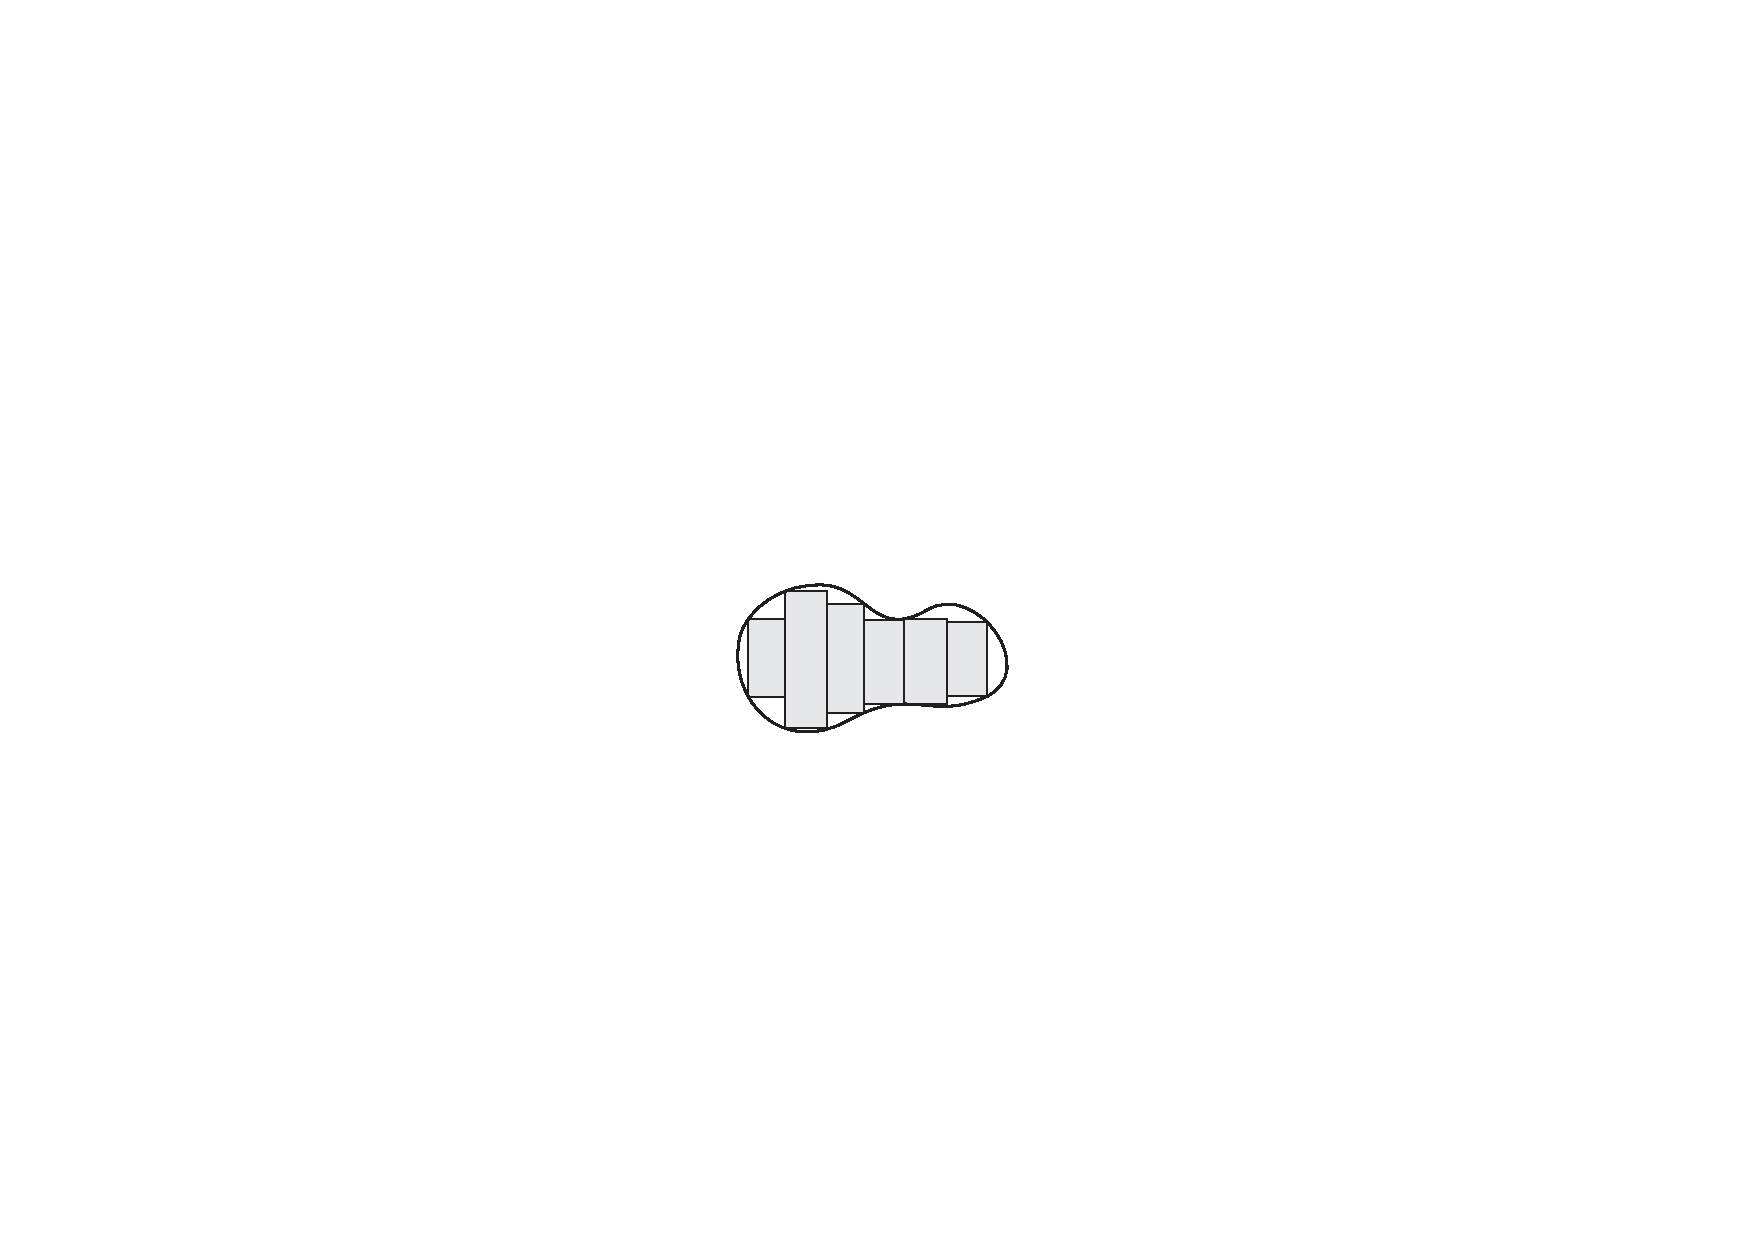
\includegraphics{T3/figs/DefArea2.pdf}
\end{center}
\end{latexonly}
\begin{rawhtml}
<div class="center">
<img src="./T3/figuras/Leccion33-4-DefArea2.svg" width="300">
</div>
\end{rawhtml}
%
De hecho, este es el punto de partida para definir las \emph{sumas de Riemann}, que introducimos a continuación, y que son el fundamento de la \emph{Integral de Riemann}.

\subsection{Sumas de Riemann: integración numérica}

Si $f$ es una función positiva en el intervalo $[a,b]$, queremos calcular el área de la región comprendida entre el grafo de $f$, el eje $OX$ y las rectas $X=a$ y $X=b$.
Este área será la integral definida de $f$ en el intervalo $[a,b]$.
%
\begin{latexonly}
\begin{center}
\begin{tikzpicture}[x=3em,y=3em]
%\pgfsetlinewidth{.5pt}
% Zona sombreada:
% Una vez generada la curva, duplico el archivo .table
% y le añado los puntos que cierran la región.
% De esta forma, puedo utilizar \fill para crear la
% región sobreada:
\fill[gray!30] plot file {T3/figs/Calc3.riemann2.table};
\draw[domain=1:5,smooth,variable=\x]
plot (\x,0.2*\x*\x*\x-1.7*\x*\x+4.0*\x-.5);
%
\draw (1,2.0) -- (1,0) node[below] {$a$};
\draw (5,2)--(5,0) node[below] {$b$};
\draw[latex-] (4,.7)--(6,1.5) node[right]{Área$=\displaystyle\int_a^b f(x)\mathrm dx$};
% Ejes
\draw[-stealth] (-.15,0) -- (5.7,0) node[right] {$X$}; 
\draw[-stealth] (0,-.15) -- (0,2.5) node[right] {$Y$};;
\end{tikzpicture}
\end{center}
\end{latexonly}
\begin{rawhtml}
<div class="center">
<img src="./T3/figuras/Leccion33-5.svg" width="400">
</div>
\end{rawhtml}
%
Con este modelo, podemos plantear fácilmente los cálculos necesarios para aproximar el valor de la integral como la suma de las áreas de varios rectángulos.
Para describir estos rectángulos, elegimos un conjunto de puntos $x_k$, tales que
\[
a=x_0 \sle x_1 \sle x_2 \sle \dots \sle x_{m-1} \sle x_m=b,
\]
y puntos intermedios $s_k$ tales que $x_{k-1}\le s_k\le x_k$, de tal forma que cada subintervalo
$[x_{k-1},x_k]$ será la base de un rectángulo y $f(s_k)$ su altura.
El área de cada rectángulo será $f(s_k)(x_k-x_{k-1})$ y por lo tanto, la aproximación del área de la región será la suma de las áreas de todos estos rectángulos, es decir
\enlargethispage{\baselineskip}
\[
\sum_{k=1}^m f(s_k)(x_k-x_{k-1}).
\]
Esta aproximación corresponde a la región sombreada que podemos ver en la figura~\ref{fig:sum-rie} y la expresión se denomina \emph{Suma de Riemann}.
\begin{rawhtml}
<div class="center">
<img src="./T3/figuras/Leccion33-6.svg" width="400">
</div>
\end{rawhtml}
%
\begin{latexonly}
\begin{figure}
\begin{center}
\begin{tikzpicture}[x=4.5em,y=4.5em]
\pgfsetlinewidth{.5pt}
% Zona sombreada (suma de Riemann)
\draw[gray!40,fill=gray!40] (1,0) -- (1,2.234375) -- (1.5,2.234375) -- (1.5,2.365625000000001) -- (2,2.365625000000001) -- (2,2.171875) -- (2.5,2.171875) -- (2.5,1.803125000000001) -- (3,1.803125000000001) -- (3,1.409375000000004) -- (3.5,1.409375000000004) -- (3.5,1.140625) -- (4,1.140625) -- (4,1.146875000000003) -- (4.5,1.146875000000003) -- (4.5,1.578125000000004) -- (5,1.578125000000004) -- (5,0) -- (1,0);
% Ejes y función:
\draw[-stealth] (-.15,0) -- (5.7,0) node[right] {$X$}; 
\draw[-stealth] (0,-.15) -- (0,2.5) node[right] {$Y$};;
\draw[thick,domain=1:5,smooth,variable=\x]
plot (\x,0.2*\x*\x*\x-1.7*\x*\x+4.0*\x-.5);
\draw (.75,-.02) node[below] {$x_0=a$};
\draw (1,2.0) -- (1,0);
\draw (1.5,2.35) -- (1.5,0) node[below] {$x_1$};
\draw (2,2.3)--(2,0)  node[below] {$x_2$};
\draw (2.5,2) -- (2.5,0) node[below] {$x_3$};
\draw (3,1.6) --(3,0) node[below]{\dots};
\draw (3.5,1.25) -- (3.5,0) node[below]{\dots}; 
\draw (4,1.1) -- (4,0);
\draw (4,-.1) node[below]{$x_{m-2}$};
\draw (4.5,1.3) -- (4.5,0) node[below]{$x_{m-1}$};
\draw (5,2)--(5,0);
\draw (5.25,-.02) node[below] {$x_m=b$};
\end{tikzpicture}
\end{center}
\caption{Aproximación del área bajo el grafo usando sumas de Riemann.}\label{fig:sum-rie}
\end{figure}
%
\begin{figure}
\begin{center}
\begin{tikzpicture}[x=7em,y=7em]
\pgfsetlinewidth{.5pt}
\draw[-stealth] (-.15,0) -- (2.3,0) node[right] {$X$}; 
\draw[-stealth] (0,-.15) -- (0,1.15) node[right] {$Y$};;
\draw[gray!40,fill=gray!40](0,0)--(0,0.4375)--(0.25,0.4375)--(0.25,0.75)--(0.5,0.75)--(0.5,0.9375)--(0.75,0.9375)--(.75,1)--(1,1)
--(1,0.9375)--(1.25,0.9375)--(1.25,0.75)--(1.5,0.75)--(1.5,0.4375)--(1.75,0.4375)--(1.75,0)--(2,0)--(0,0);
\draw[thick,domain=0:2] plot (\x,2*\x-\x*\x);
%plot[id=parab8,samples=50]
%function{2*x-x*x};
\end{tikzpicture}
\end{center}
\caption{Aproximación del área del ejemplo~\ref{ej-riemann}.}\label{fig:ej-riemann}
\end{figure}
\end{latexonly}
\begin{ejemplo}\label{ej-riemann}
%
Consideremos la función $f(x)=2x-x^2$ en el intervalo $[0,2]$ y
consideremos los puntos $x_k=\dfrac{k}4$, $s_k=\dfrac{k}4$ para cada $k=0,1,\dots,8$;
con ellos, vamos a calcular una aproximación del área que queda debajo de la gráfica de $f$, según aparece en la figura~\ref{fig:ej-riemann}.
\begin{rawhtml}
<div class="center">
<img src="./T3/figuras/Leccion33-7.svg" width="400">
</div>
\end{rawhtml}
En primer lugar, observamos que, para cada $k=1,\dots,8$
\enlargethispage{-1.2ex}
\[
x_k-x_{k-1} = \frac{k}4 - \frac{k-1}4 = \frac14,
\]
y por lo tanto
\begin{multline*}
\sum_{k=1}^m f(s_k)(x_k-x_{k-1})
= \sum_{k=1}^8 f\big(\frac{k}4\big)\frac14
= \frac14\sum_{k=1}^8 \big(2\frac{k}4-\frac{k^2}{16}\big)=\\
= \frac14\big(\big(\frac{1}2-\frac{1^2}{16}\big) +
 \big(\frac{2}2-\frac{2^2}{16}\big) +
 \big(\frac{3}2-\frac{3^2}{16}\big) +
 \big(\frac{4}2-\frac{4^2}{16}\big) +\\
 +\big(\frac{5}2-\frac{5^2}{16}\big) +
 \big(\frac{6}2-\frac{6^2}{16}\big) +
 \big(\frac{7}2-\frac{7^2}{16}\big) +
 \big(\frac{8}2-\frac{8^2}{16}\big)\big) =\frac{21}{16}\tag*{\fej}
\end{multline*}
\end{ejemplo}

Las aproximaciones dadas por las sumas de Riemann pueden ser mejoradas aumentando el número de puntos, de forma que la amplitud de todos los subintervalos disminuya tendiendo a 0.
Decimos que una función es integrable si, en estas condiciones, las sumas de Riemann convergen a un mismo valor y este valor se denomina \emph{integral (definida)} de la función en el intervalo.

\begin{ejemplo}\label{ej-parab}
Vamos a considerar nuevamente la función $f(x)=2x-x^2$ del ejemplo anterior.
Pero ahora, vamos a calcular las sumas de Riemann para una partición en $n$ subintervalos iguales, es decir, de amplitud $\dfrac2n$, y tomando igualmente el extremo superior como punto intermedio de cada subintervalo;
es decir, $s_{n,k}=x_{n,k} = \dfrac{2k}n$ para $k=1,\dots,n$ y entonces,
\begin{align*}
\sum_{k=1}^n f(s_{n,k})(x_{n,k}-x_{n,k-1})
& = \frac2n\sum_{k=1}^n f(s_{n,k}) = \frac2n\sum_{k=1}^n f(\frac{2k}n)=\\
& = \frac2n \sum_{k=1}^n \big(2\frac{2k}n-\frac{4k^2}{n^2}\big)= \\
& = \left(\left( \frac8{n^2}\sum_{k=1}^n k\right) -\left( \frac8{n^3}\sum_{k=1}^n k^2\right)\right)=\\
& = \left(\left( \frac8{n^2}\frac{n(n+1)}2\right) -\left( \frac8{n^3}\frac{n(n+1)(2n+1)}6\right)
\right)=\\
& =\frac{4n^2-4}{3n^2}
\end{align*}
Entonces,
\[
\int_0^2(2x-x^2)\mathrm dx = \lim \frac{4n^2-4}{3n^2} =\frac43\tag*{\fej}
\]
%Ahora podemos comparar este resultado con la aproximación obtenida en el ejemplo~\ref{ej-riemann}:
%\[
%\text{Error}=\frac43-\frac{21}{16} =\frac1{48} = 0.0208 \wideparen3 
%\]
\end{ejemplo}

%Si la función es positiva en el intervalo, el valor de esta integral es el área de la región que queda entre el grafo y el eje~$OX$.

En particular, las funciones continuas son integrables en cada intervalo cerrado contenido en su dominio y estas funciones serán con las que trabajaremos en el curso.
Para calcular integrales definidas usamos el cálculo de primitivas (si es posible) y usamos las sumas de Riemann como método de aproximación.
No obstante, debemos entender que la teoría asociada a las sumas de Riemann no es solo importante como método de aproximación, sino que además es la forma de probar que una magnitud puede definirse o calcularse mediante integrales: cualquier magnitud que se puede aproximar por sumas de Riemann de una función continua, tiene a la integral como valor exacto; más adelante, veremos algunos ejemplos intuitivos de estas ideas.

\begin{rawhtml}
<p style="text-align: center;"><iframe width="560" height="316" src="https://www.youtube.com/embed/rWzW0uggaN0?list=PL2rtpLKW91qawRYK1FOQv2H_dcdGz_dIo" frameborder="0" allowfullscreen=""></iframe></p>
\end{rawhtml}


\subsection{Regla de Barrow y propiedades}

Ya hemos recordado en la primera lección de este tema el teorema fundamental de cálculo, que establece que si $f$ es continua, la función
\[
F(x)=\int_a^x f(t)\mathrm dt,
\]
es una primitiva de $f$, es decir, $F'(x)=f(x)$.
A partir de este teorema se deduce fácilmente la Regla de Barrow, que es la herramienta para cálculo de integrales basada en primitivas.
Supongamos que $G$ es cualquier primitiva de $f$, que habremos hallado usando los métodos vistos en la primera lección de este tema.
Entonces $F$ y $G$ se diferencian en una constante,
\begin{equation}\label{eq:barrow1}
G(x)-\int_a^x f(t)\mathrm dt = C, \text{ para todo } x\in[a,b]
\end{equation}
En particular, tomando $x=a$ determinamos el valor de $C$:
\[
C=G(a)-\int_a^a f(t)\mathrm dt = G(a)
\]
y con él, ya podemos expresar el valor de la integral definida en terminos de $G$:
\[
\int_a^x f(t)\mathrm dt = G(x)-G(a).
\]
De esta forma, hemos demostrado la regla de Barrow.
%
\begin{teorema}[Regla de Barrow]\label{th:barrow}
Si $f$ es continua en $[a,b]$ y $G'(x)=f(x)$ para todo $x\in[a,b]$, entonces 
\[ 
\int_a^b f(t)\,\mathrm dt=G(b)-G(a) \stackrel{\text{(Notación)}}{=} \left[G(x)\vphantom{\dfrac12}\right]_a^b
\]
\end{teorema}
\begin{rawhtml}
&nbsp;
\end{rawhtml}
\begin{ejemplo}
Vamos a calcular de nuevo el área de la región del ejemplo~\ref{ej-parab} usando la regla de Barrow:
\begin{equation}
\int_0^2 (2x-x^2)\mathrm dx = \left[x^2-\frac{x^3}3\right]_0^2 = 4-\frac83=\frac43\tag*{\fej}
\end{equation}
\end{ejemplo}
\begin{rawhtml}
&nbsp;
\end{rawhtml}
\begin{ejemplo}\label{ej-circ}
El área de un círculo se puede calcular a partir de la gráfica de la función $f(x)=\sqrt{r^2-x^2}$. Si consideremos el intervalo $[0,r]$, la región entre el grafo de $f$ y el eje $OX$ es un cuarto de círculo y por lo tanto:
\[
A=4\int_0^r\sqrt{r^2-x^2}\mathrm dx
\]
Hallamos en primer lugar la primitiva:
\begin{align*}
A =& 4\int \sqrt{r^2-x^2}\mathrm dx=\\
&\left[
\begin{array}{l}
x=r\operatorname{sen}\theta %\text{ (esta función es creciente en $[0,\pi/2]$)}\\
\mathrm dx=r\cos\theta d\theta
\end{array}
\right.\\
=& 4\int \sqrt{r^2-r^2\operatorname{sen}^2\theta}\, r\cos\theta\, d\theta=\\
= & 4\int r^2\cos^2\theta d\theta
= 4r^2\int \left(\frac12+\frac12\cos2\theta\right) d\theta=\\
= & 4r^2\left(\frac{\theta}2+\frac14\operatorname{sen} 2\theta\right)
= r^2\left(2\theta +\operatorname{sen} 2\theta\right)=\\
= & r^2\Big(2\operatorname{arcsen}\frac{x}{r} +\operatorname{sen} 2(\operatorname{arcsen}\frac{x}{r})\Big)
\end{align*}
Por lo tanto
\begin{multline*}
A=4\int_0^r\sqrt{r^2-x^2}\mathrm dx=
\left[r^2\Big(2\operatorname{arcsen}\frac{x}{r} +\operatorname{sen} 2(\operatorname{arcsen}\frac{x}{r})\Big)\right]_0^r=\\
=r^2\Big(2\operatorname{arcsen} 1 +\operatorname{sen} 2(\operatorname{arcsen} 1)\Big)
-r^2\Big(2\operatorname{arcsen} 0 +\operatorname{sen} 2(\operatorname{arcsen} 0)\Big)=\\
=r^2\Big(2\frac{\pi}2 +\operatorname{sen} 2(\frac{\pi}2)\Big)
=\pi r^2\tag*{\fej}
%\left[2r^2\operatorname{arcsen}\dfrac{x}r +2x\sqrt{r^2-x^2}\right]_0^r=\pi r^2
\end{multline*}
\end{ejemplo}

Debemos insistir en que el hecho de tener un resultado tan potente como la Regla de Barrow para calcular integrales definidas, no debe llevarnos a la conclusión errónea de que podemos olvidar la definición de integral.
De hecho, la regla de Barrow solo es útil para aquellas funciones que admiten una primitiva \emph{expresable en términos de funciones elementales}, y ya sabemos que no todas las funciones continuas admiten este tipo de primitivas.

\begin{teorema}[Linealidad de la integral]
Si $f$ y $g$ son continuas en $[a,b]$ y $\alpha,\beta\in\mathbb{R}$, entonces:
\[
\int_a^b(\alpha f(x)+\beta g(x))\,\mathrm dx=
\alpha\int_a^b f(x)\,\mathrm dx +\beta \int_a^b g(x)\,\mathrm dx
\]
\end{teorema}
\begin{rawhtml}
&nbsp;
\end{rawhtml}
\begin{teorema}[Propiedad de aditividad] Sea $f$ una función continua en $[a,b]$ y
$c\in[a,b]$, entonces
\[
\int_a^b f(x)\,\mathrm dx =\left(\int_a^c f(x)\,\mathrm dx\right)+
\left(\int_c^b f(x)\,\mathrm dx\right)
\]
\end{teorema}
%
Tal y como hemos definido la integral, en el operador $\displaystyle\int_a^b$ es necesario que $a\le b$.
Para flexibilizar los cálculos, es conveniente admitir la situación inversa.
%
\begin{definicion}
Si $f$ es continua en $[a,b]$, definimos la integral
$\displaystyle\int_b^af(x)\,\mathrm dx$ como:
\[
\int_b^a f(x)\,\mathrm dx = -\int_a^b f(x)\,\mathrm dx
\]
\end{definicion}

Esta definición se hace así para que la extensión del operador siga verificando la propiedad de aditividad
\begin{align*}
& \int_a^bf(x)\,\mathrm dx+\int_b^af(x)\,\mathrm dx = \int_a^a f(x)\,\mathrm dx =0\\
& \int_a^bf(x)\,\mathrm dx+\int_b^af(x)\,\mathrm dx = \int_a^bf(x)\,\mathrm dx-\int_a^bf(x)\,\mathrm dx = 0
\end{align*}

A continuación, vamos a dar los enunciados de los teoremas de cambio de variable e integración por partes, pero para integrales definidas.
Si utilizamos estos métodos para calcular integrales definidas, es preferible usarlos tal y como los enunciamos a continuación ya que, como veremos en los ejemplos, su aplicación simplifica los cálculos necesarios.
%
\begin{teorema}[Cambio de variable directo]\label{th:sust1}
Supongamos que $g'$ es continua y en $[a,b]$ y que $f$ es continua y biyectiva entre $g(a)$ y $g(b)$,
entonces:  
\[
\int_a^bf(g(x))g'(x)\mathrm dx = \int_{g(a)}^{g(b)}f(u)\mathrm du
\]
\end{teorema}
\begin{rawhtml}
&nbsp;
\end{rawhtml}
\begin{corolario}[Cambio de variable inverso]\label{th:sust2}
Sea $f$ una función continua en $[\alpha ,\beta]$.
Consideremos una función $g\colon I\to [\alpha ,\beta]$ biyectiva, continua y con primera derivada continua. Entonces, 
\[
\int_\alpha^\beta f(x)\mathrm dx = 
\int_{g^{-1}(\alpha)}^{g^{-1}(\beta)}f(g(u))g'(u)\mathrm du
\]
\end{corolario}

Obsérvese que, en este teorema, hemos incluido, como condición necesaria, que el cambio de variable esté dado por una función biyectiva, es decir, monótona en el intervalo de integración.
%
\begin{ejemplo}
Vamos a repetir el cálculo del área de un círculo de radio $r$, que hicimos anteriormente, pero de forma más simple por la ayuda del resultado anterior:
\begin{align*}
A =& 4\int_0^r\sqrt{r^2-x^2}\mathrm dx=\\
&\left[
\begin{array}{l}
x=r\operatorname{sen}\theta \text{ (esta función es creciente en $[0,\pi/2]$)}\\
\mathrm dx=r\cos\theta d\theta\\
x_0=0 \Rightarrow \theta_0=\operatorname{arcsen} 0 = 0\\
x_1=r \Rightarrow \theta_1=\operatorname{arcsen}\frac{r}r =\operatorname{arcsen}1 = \pi/2\\
\end{array}
\right.\\
= & 4\int_0^{\pi/2}r^2\cos^2\theta d\theta
= 4r^2\int_0^{\pi/2}\left(\frac12+\frac12\cos2\theta\right) d\theta=\\
= & 4r^2\left[\frac{\theta}2+\frac14\operatorname{sen} 2\theta\right]_0^{\pi/2}
= 4r^2 \dfrac{\pi}4 = \pi r^2\tag*{\fej}
\end{align*}
\end{ejemplo}
\begin{rawhtml}
&nbsp;
\end{rawhtml}
\begin{teorema}[Integración por partes]\label{th:partes}
Sean $f$ y $g$ dos funciones tales que $f'$ y $g'$ son  continuas, entonces:
\[
\int_a^bf(x)g'(x)\mathrm dx = \left[f(x)g(x)\vphantom{\frac12}\right]_a^b-\int_a^bg(x)f'(x)\mathrm dx
\]
\end{teorema}
\begin{rawhtml}
&nbsp;
\end{rawhtml}
\begin{ejemplo}
Utilizamos el resultado anterior para calcular la siguiente integral definida
\[
\int_{\pi/6}^{\pi/2}\cos x \log\operatorname{sen} x\,\mathrm dx
\]
Para ello, utilizamos el cambio de variable
\[
t = \operatorname{sen} x,\quad
\mathrm dt = \cos x\,\mathrm dx
\]
Los límites de integración se modifican de la siguiente forma: para $x=\pi/6$, el valor de $t$ es  $1/2$, mientras que para $x=\pi/2$ el valor de $t$ es 1.
%
\begin{align*}
\int_{\pi/6}^{\pi/2}\cos x & \log\operatorname{sen} x\,\mathrm dx =\int_{1/2}^{1} \log t\,\mathrm dt \\
& \left[
\begin{array}{l}
u= \log t \Longrightarrow \mathrm du=\dfrac{\mathrm dt}t \\
\mathrm dv =\mathrm dt \Longrightarrow v=t
\end{array}
\right.\\
= & \left[t\log t\vphantom{\dfrac12}\right]_{1/2}^{1} - \int_{1/2}^{1}\mathrm dt 
= \dfrac{-\log(1/2)}2-\left[t\vphantom{\dfrac12}\right]_{1/2}^{1} = \dfrac{\log 2}2-\dfrac12
\end{align*}
\end{ejemplo}

\begin{rawhtml}
<p style="text-align: center;"><iframe width="560" height="316" src="https://www.youtube.com/embed/aWZcsLIVAAM?list=PL2rtpLKW91qawRYK1FOQv2H_dcdGz_dIo" frameborder="0" allowfullscreen=""></iframe></p>
\end{rawhtml}


\subsection{Aplicaciones geométricas}\label{sec:geom}

Aunque hemos utilizado el cálculo de áreas de regiones planas para motivar el concepto de integral, debemos tener en cuenta que una integral se identifica con un área solo si el integrando es una función positiva.
%
\begin{teorema}
Si $f$ es una función continua y positiva en el intervalo
$[a,b]$, entonces la integral definida $\displaystyle\int_a^b f$ es el valor del área de la región comprendida entre el grafo de $f$ y el eje $OX$ en dicho intervalo.
\end{teorema}

A continuación, repasamos otras aplicaciones de la integral para determinar otras magnitudes, como volúmenes, longitudes de curvas o áreas de superficies alabeadas.
Otras aplicaciones posibles se encuentran en el campo de la física, para calcular el trabajo o los centros de masas.

\paragraph{Cálculo de volúmenes por secciones.}
Supongamos que tenemos el sólido acotado
por dos planos perpendiculares a una recta y que para cada $t\in[a,b]$ conocemos el área $A(t)$, de las secciones del sólido perpendiculares a dicha recta, de tal forma que la función $A$ es continua.
Si tomamos una partición del intervalo, $a=t_0\sle t_1\sle \dots\sle t_n=b$, el volumen del sólido se puede aproximar por la suma de los volúmenes de los cilindros de base $A(t_i)$ y altura $(t_i-t_{i-1})$:
\[
V\approx \sum_{i=1}^n A(t_i)(t_i-t_{i-1})
\]
Obviamente, estas expresiones son sumas de Riemann asociadas a la función $A(t)$, y por lo tanto, podemos afirmar que el volumen exacto es:
\[
V=\int_a^b A(t)\mathrm dt
\]
En algunos casos, el enunciado del problema dará la posición del sólido
respecto de los ejes coordenados, pero más frecuentemente, tendremos que elegir
nosotros esta posición, de tal forma que sea fácil calcular las áreas
$A(t)$.

\begin{ejemplo}\label{ej-cunna}
Se corta una cuña de un tronco (cilíndrico) de radio 2 dm
dando dos cortes con una sierra mecánica que llegan hasta el centro del
tronco. Si uno de los cortes se hace perpendicular y el otro formando un ángulo de
$30^\circ$ con  el primero, ¿qué volumen tendrá la cuña?
\begin{latexonly}
\begin{center}
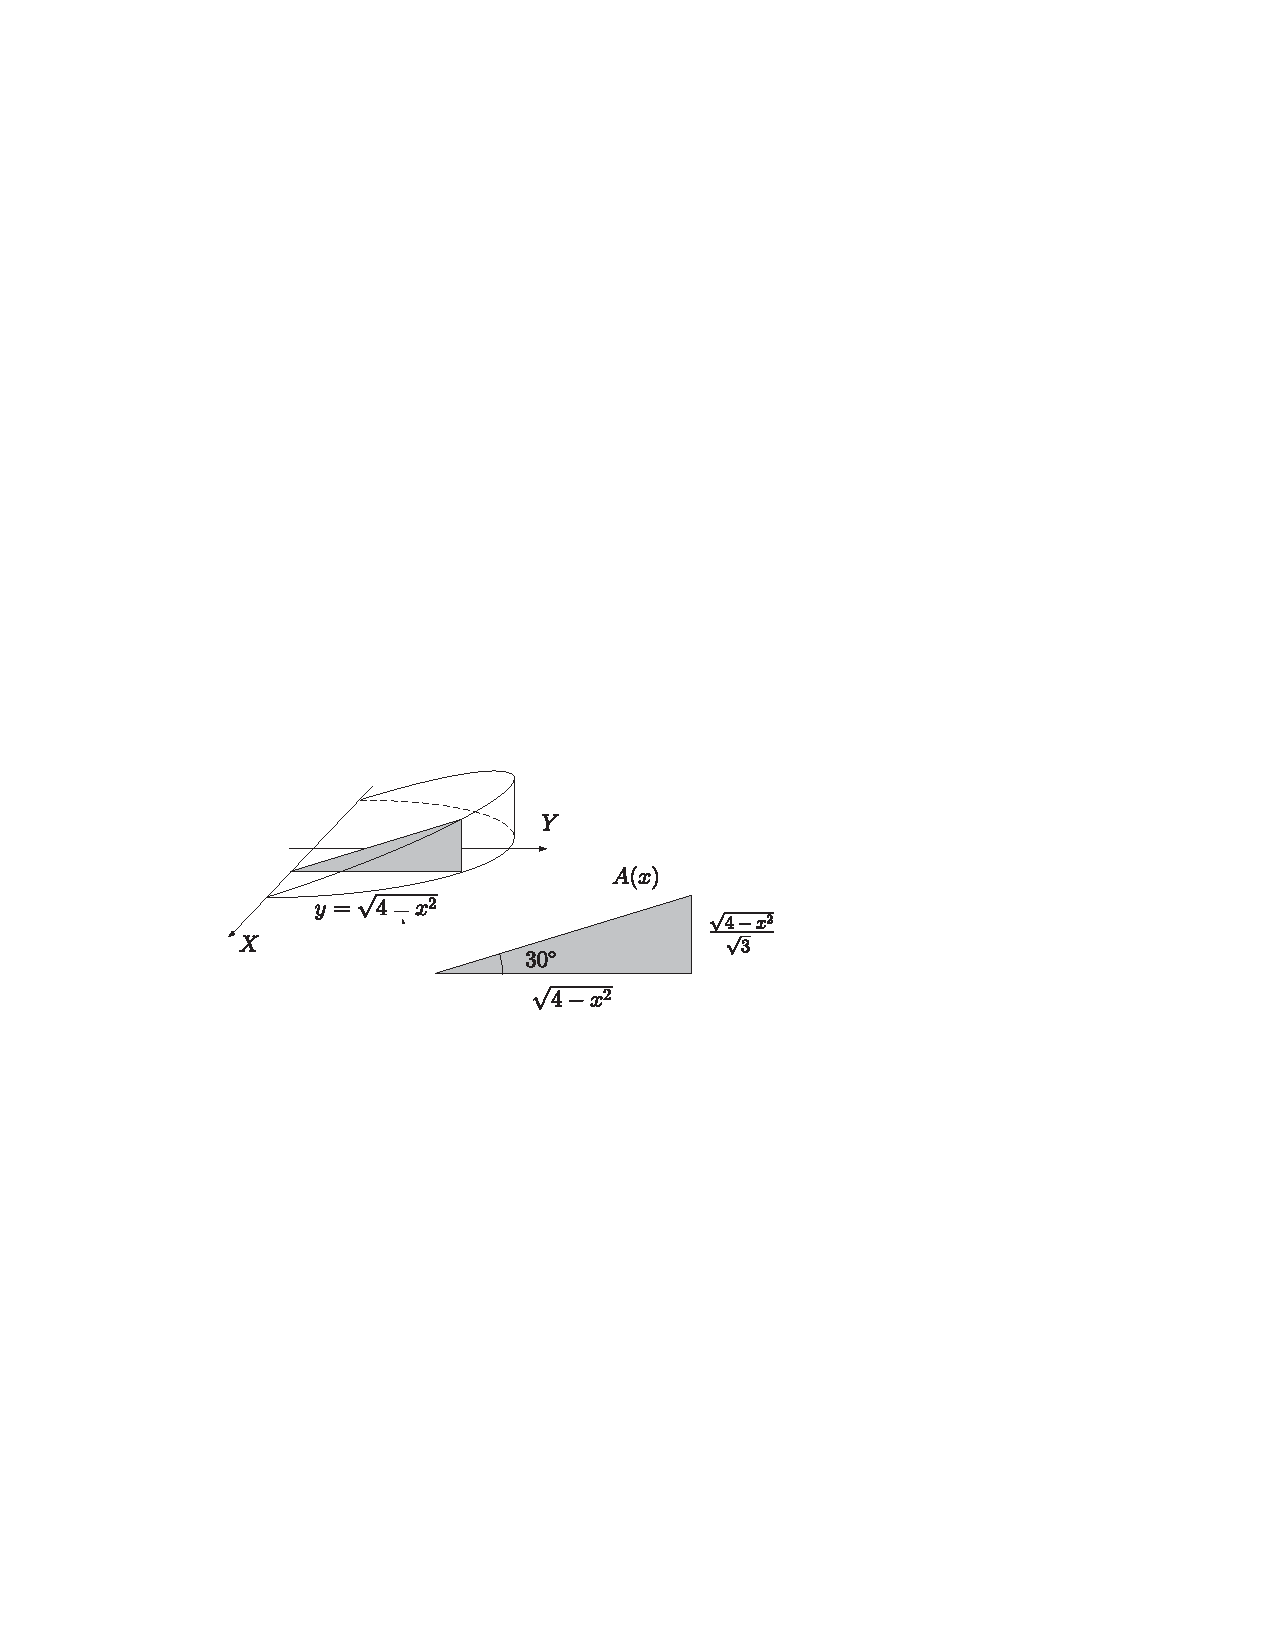
\includegraphics{T3/figs/cunna.pdf}
\end{center}
\end{latexonly}
\begin{rawhtml}
<div class="center">
<img src="./T3/figuras/Leccion33-8-cunna.svg" width="500">
</div>
\end{rawhtml}
Para hacer el cálculo utilizando el método de las secciones, situamos el sólido como se muestra en la figura. La base de la cuña, perpendicular al eje del tronco, es el interior del semicírculo $y=\sqrt{4-x^2}$.
Al hacer los cortes perpendiculares al eje $OX$, las secciones son triángulos rectángulos cuya base es $\sqrt{4-x^2}$ y forma un ángulo de $30^\circ$ con la hipotenusa.
Por lo tanto, su altura es $\frac{\sqrt{4-x^2}}{\sqrt3}$ y el área de la sección es 
$A(x)=\frac1{2\sqrt3}(4-x^2)$. El volumen que queríamos calcular es:
\begin{equation}
V=\int_{-2}^2 A=\int_{-2}^2 \frac{4-x^2}{2\sqrt3}\mathrm dx
=\dfrac{\sqrt3}6 \left[4x-\dfrac{x^3}3\right]_{-2}^2 = \dfrac{16}9\sqrt3
\tag*{\fej}
\end{equation}
\end{ejemplo}

%:Arreglar: expresarlo de una forma más general
% \pi(R(t)^2-r(t)^2)

Como caso particular, podemos calcular el volumen de \emph{sólidos de revolución} usando el método de los discos.
Si consideremos una región plana determinada por el grafo de una función
continua $f$ entre $a$ y $b$ que gira alrededor del eje $OX$,
el sólido generado verifica que las secciones perpendiculares al
eje $OX$, son circulos de radio $f(x)$. Por tanto, el volumen del sólido es:
\[
V=\int_a^b \pi f(x)^2\,\mathrm dx
\]

\paragraph{Cálculo de volúmenes de revolución por capas.}
Otra forma de generar un sólido de revolución es girando la región determinada por una función continua en un intervalo $[a,b]$ con $a\geq 0$, alrededor del eje $OY$. Para aproximar el valor de este volumen, consideremos una partición $a=x_0\sle x_1\sle \dots\sle x_n=b$, y los puntos intermedios $s_i=\frac{x_i+x_{i-1}}2$;
el volumen del sólido se puede aproximar por la suma de los volúmenes de los cilindros cuya base es la corona circular de radios $x_{i-1}$ y $x_i$ y cuya altura es $f(x_i)$:
\begin{multline*}
V \approx \sum_{i=1}^n f(s_i)(\pi x_i^2-\pi x_{i-1}^2) =
\sum_{i=1}^n \pi f(s_i) (x_i+x_{i-i})(x_i-x_{i-i}) = \\ =
\sum_{i=1}^n 2 \pi f(s_i) s_i (x_i-x_{i-i})
\end{multline*}
%
Obviamente, estas expresiones son sumas de Riemann asociadas a la función $2\pi xf(x)$, que es continua por serlo $f$.
Por lo tanto, podemos afirmar que el volumen exacto es
\[
V=\int_a^b 2\pi xf(x)\,\mathrm dx
\]
%
%El método de las secciones es adecuado para sólidos que no presentan \emph{perforaciones}, en estos casos será más recomendable utilizar el método de las capas.

%Para calcular un volumen utilizando cualquiera de los dos métodos, tendremos que situar la región (desplazándola o girándola) en los ejes de coordenadas de tal forma que el cálculo de las secciones o de las capas sea lo más simple posible.

%:Arreglar: expresarlo de una forma más general
% 2\pi*R(t)*h(t), en donde R(t) es el radio de la capa, o distancia al eje,
% y h(t) es la altura de la capa

\paragraph{Longitud de una curva parametrizada.} Si $\gamma(t)=(x(t),y(t))$ es una curva parametrizada diferenciable tal que $x'$ e $y'$ son continuas en $[a,b]$, su longitud viene dada por la siguiente integral:
\[
\ell=\int_a^b\sqrt{(x'(t))^2+(y'(t))^2}\,\mathrm dt
\]
En particular, la \emph{longitud del grafo de una función} $f$, en un intervalo $[a,b]$ es:
\[
L=\int_a^b \sqrt{1+[f'(x)]^2}\,\mathrm dx
\]

\newpage
\thispagestyle{empty}

\ 

\vfill
%\begin{center}
%(Esta página se ha dejado intencionalmente en blanco)
%\end{center}
\newpage


\section{Integración doble} %múltiple

%:Arreglar: Añadir ejemplos de integración doble, prácticamente no hay.

Consideremos un campo escalar $f\colon R\subset\mathbb{R}^2\to \mathbb{R}$ y supongamos que $f$ es positiva
y acotada en el \emph{rectángulo} $R=[a,b]\times[c,d]$. De la misma forma que para las funciones de una variable utilizábamos rectángulos, ahora podemos intentar aproximar el volumen de la región que queda entre el grafo de $f$ y el plano $XY$ tomando prismas.
La manera más simple de hacerlo es tomando particiones de los intervalos $[a,b]$ y $[c,d]$ y considerando, como base de los prismas, los rectángulos que forman:
\begin{latexonly}
\begin{center}
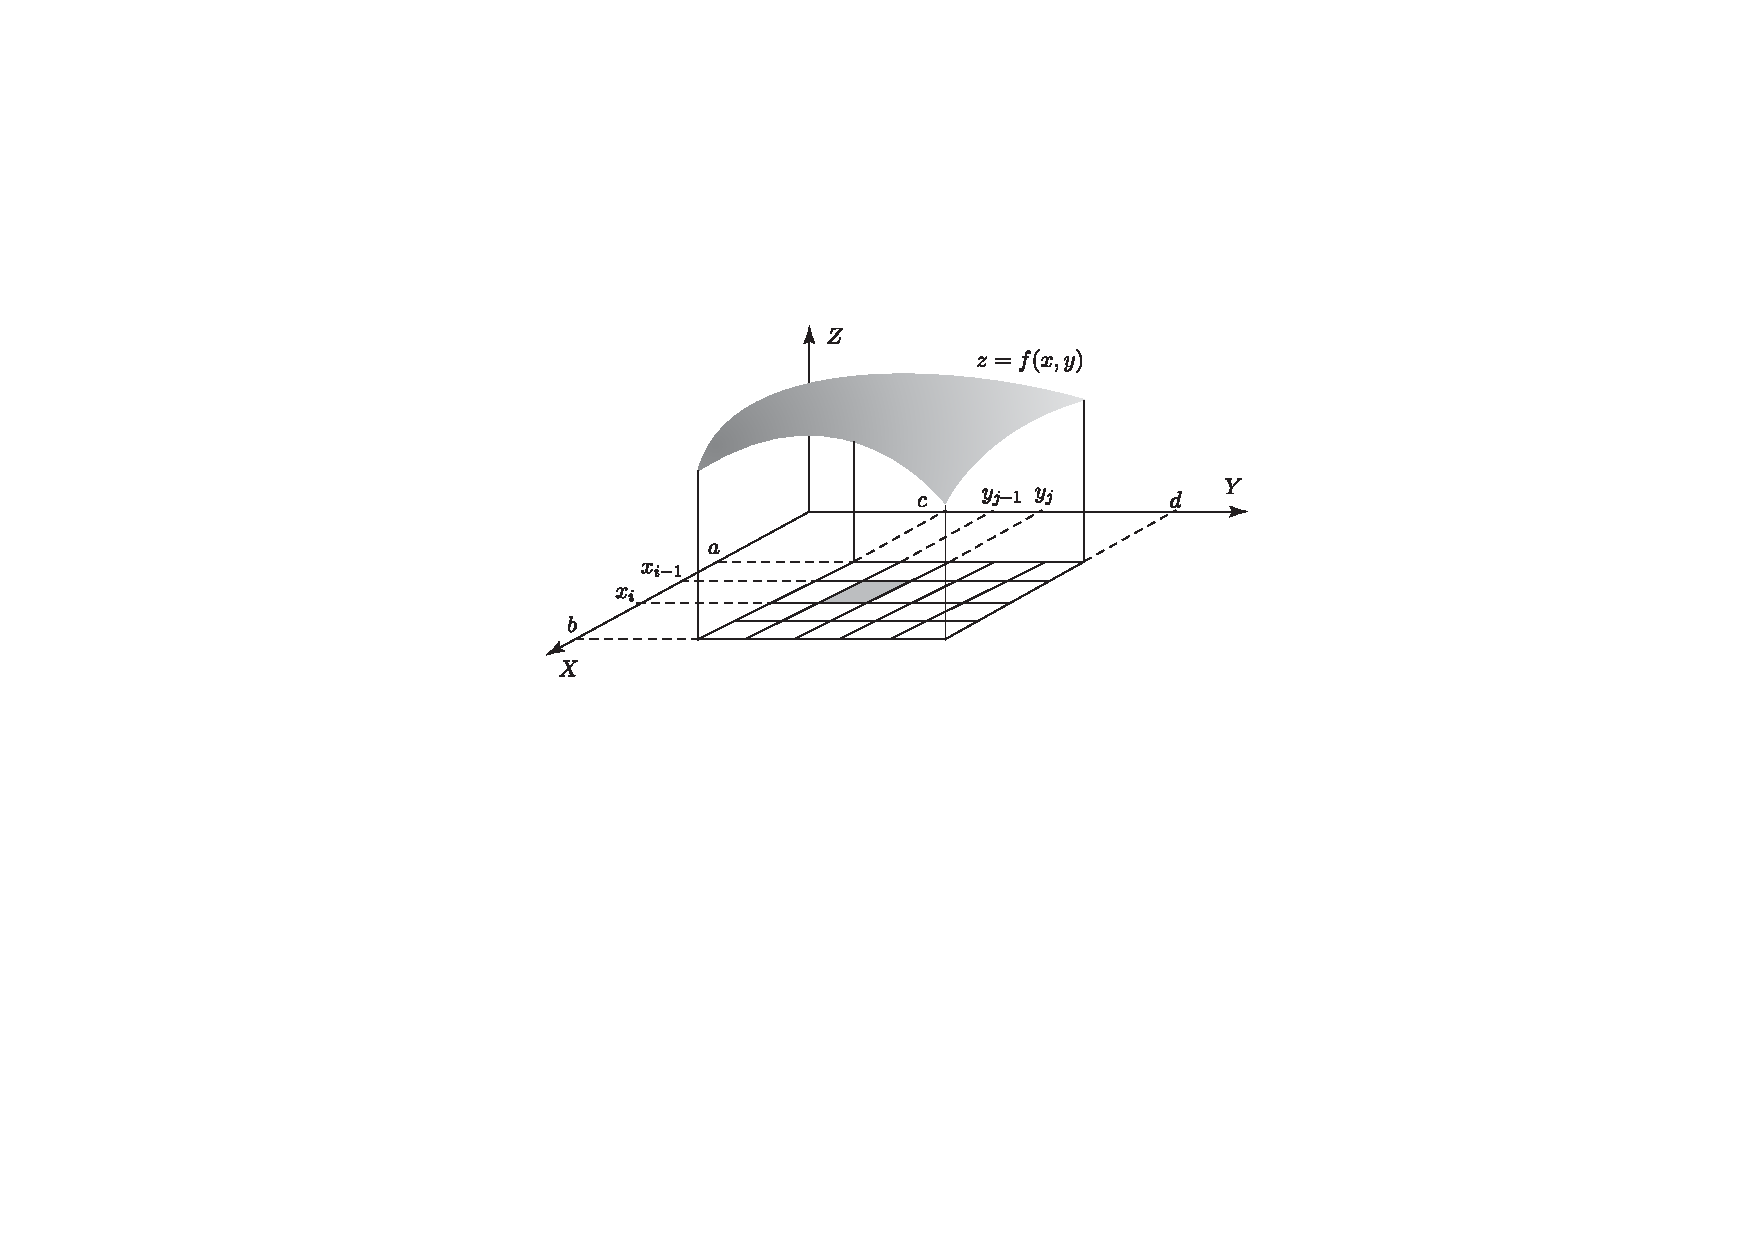
\includegraphics[scale=.8]{T3/figs/IntDoble1.pdf}\\
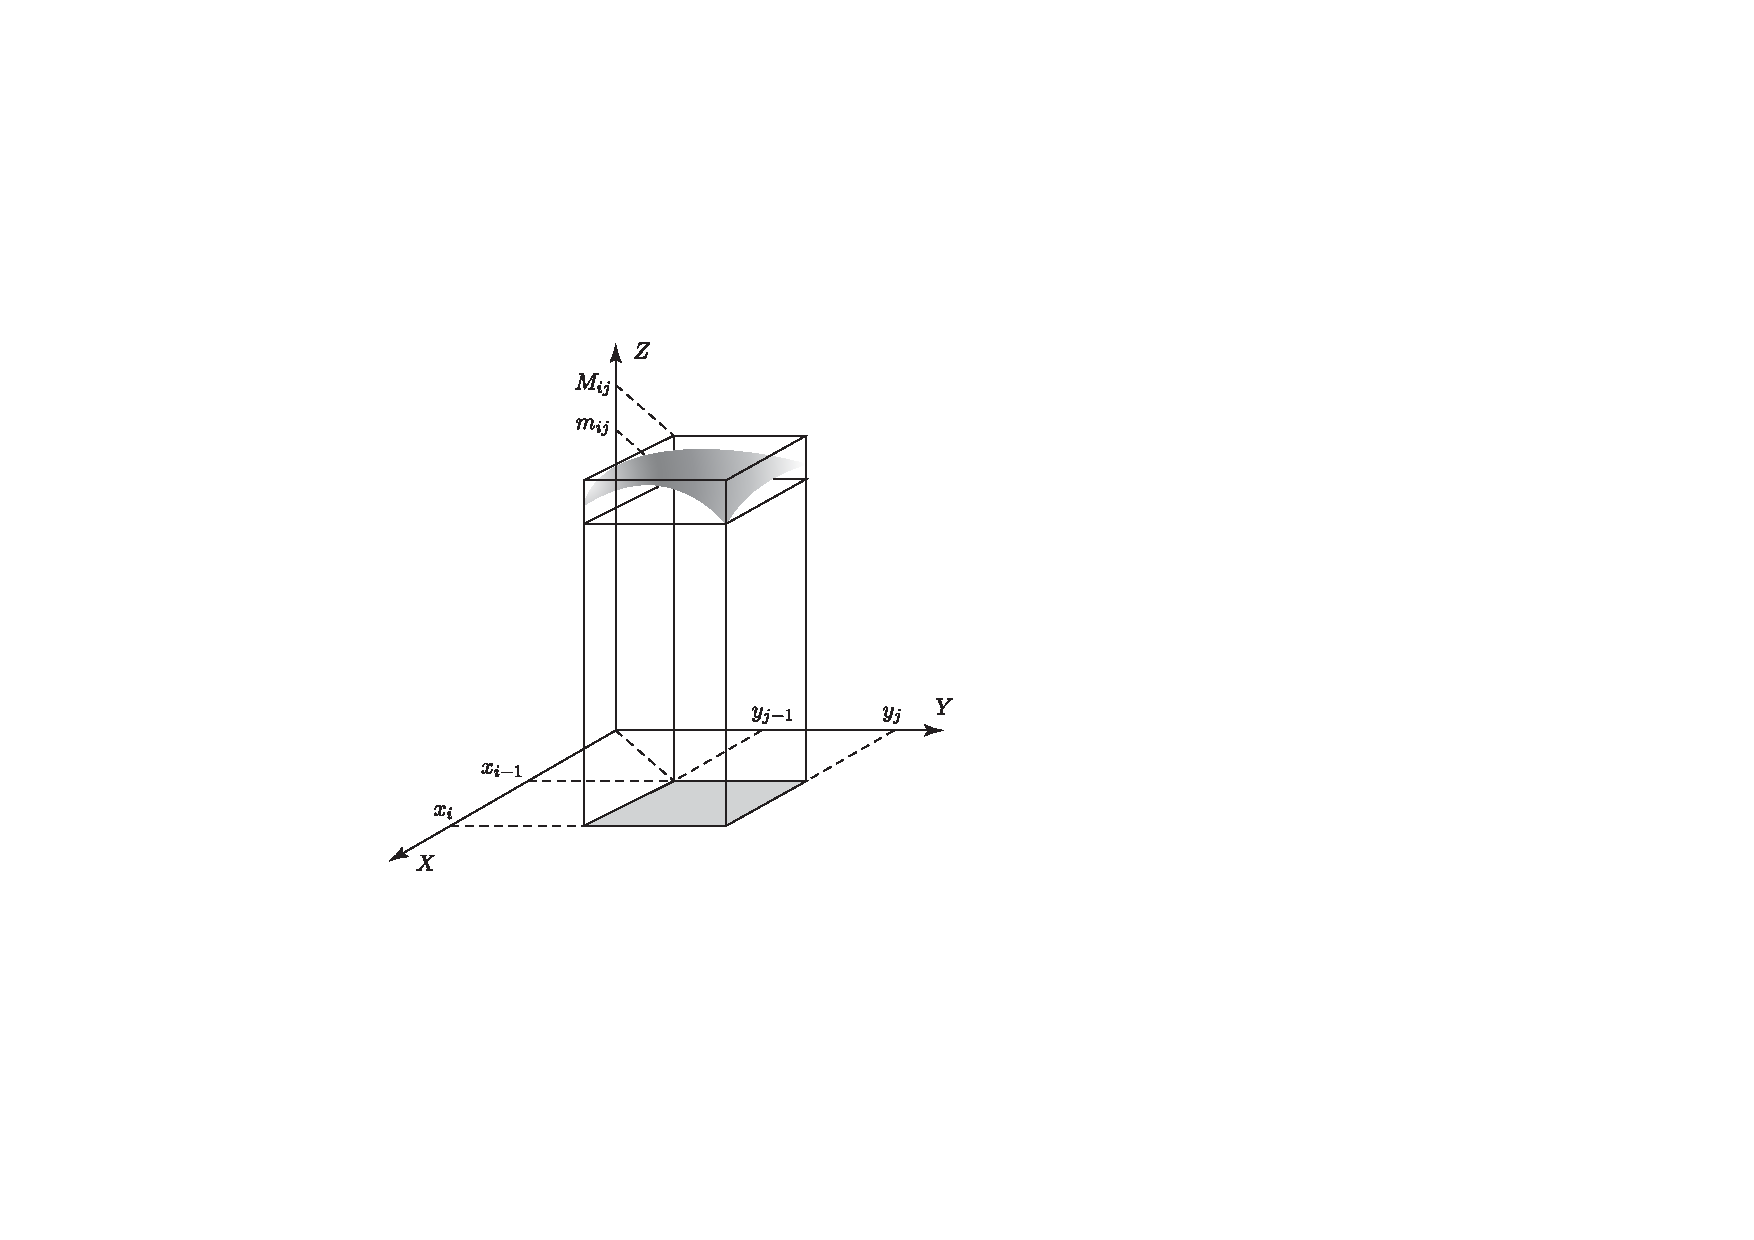
\includegraphics[scale=.8]{T3/figs/IntDoble2.pdf}
\end{center}
\end{latexonly}
\begin{rawhtml}
<div class="center">
<img src="./T3/figuras/Leccion34-1-IntDoble1.svg" width="400">
</div>
<div class="center">
<img src="./T3/figuras/Leccion34-2-IntDoble2.svg" width="400">
</div>
\end{rawhtml}

Podemos tomar aproximaciones por defecto o por exceso considerando los valores máximo y mínimo en el rectángulo como altura del prisma, o tomar una suma de Riemann usando como altura el valor de la función evaluando en cualquier punto interior.
\[
\sum_{i=1}^n\sum_{j=1}^m f(t_i,s_j)(x_i-x_{i-1})(y_j-y_{j-1}),
\]
Como para las funciones de una variable, para mejorar estas aproximaciones basta con tomar más puntos en las particiones, de forma que las áreas de los rectángulos
$R_{ij}=[x_{i-1},x_i]\times[y_{j-1},y_j]$ disminuyan tendiendo a 0.
Diremos que el campo es integrable si, en estas condiciones, las sumas de Riemann convergen a un mismo valor, que denominamos integral de $f$ en la región $R=[a,b]\times[c,d]$:
\[
\iint_Rf(x,y)\mathrm dx\mathrm dy = \lim_{\mathrm{\acute{A}rea}(R_{ij})\to 0} \sum_{i=1}^n\sum_{j=1}^m f(t_i,s_j)(x_i-x_{i-1})(y_j-y_{j-1})
\]
Si el campo es positivo en la región, esta integral es el volumen de la región que queda entre el grafo y el plano $XY$.
En este curso, solo vamos a trabajar con campos continuos, que en particular son integrables, en cualquier región contenida en su dominio.
%
%\begin{ejemplo}
%Vamos a calcular la integral del campo $f(x,y)=2x+y$ en la región $R=[0,1]\times[0,1]$ utilizando particiones regulares de $[0,1]$ en $n$ subintervalos en cada coordenada, y tomando como puntos intermedios los vértices superiores derechos de cada rectángulo.
%\begin{align*}
%\sum_{i=1}^n\sum_{j=1}^n \Big(2\frac{i}{n}+\frac{j}{n}\Big)&\frac{1}{n}\cdot\frac{1}{n}
% =\frac{1}{n^3}\sum_{i=1}^n\sum_{j=1}^n (2i+j)= \frac{1}{n^3}\sum^n_{j=1}\sum^n_{i=1} (2i+j)=\\
%& =\frac{2}{n^3}\Big(\sum^n_{j=1}\sum^n_{i=1} i \Big)
%+\frac{1}{n^3} \Big(\sum^n_{i=1}\sum^n_{j=1} j \Big)=\\
%& =\frac{2}{n^3}\Big(n\cdot\sum^n_{i=1} i \Big)
%+\frac{1}{n^3} \Big(n\cdot \sum^n_{j=1} j \Big)=\\
%& =\frac{2}{n^2}\Big(\sum_{i=1}^n i\Big)
%+\frac{1}{n^2}\Big(\sum_{j=1}^n j\Big)= \\
%& = \frac{3}{n^2}\sum_{i=1}^n i =\frac{3n(n+1)}{2n^2}=\frac{3(n+1)}{2n}
%\end{align*}
%Por lo tanto,
%$\displaystyle\int\limits_R (2x+y)\mathrm dx\mathrm dy = \lim \frac{3(n+1)}{2n}=
%\dfrac{3}{2}$\fej
%\end{ejemplo}

No vamos a abordar en este curso las integrales de campos de tres o más variables, aunque teóricamente su definición no supone ninguna dificultad.
Como veremos a lo largo del tema, el calculo de las integrales múltiples se sustenta en el cálculo de primitivas y en el estudio y transformación de las regiones de integración y por lo tanto, el nivel de dificultad que aporta el aumento de las variables no está en el propio concepto de integral sino en la manipulación de regiones y objetos en el espacio.

\begin{rawhtml}
<p style="text-align: center;"><iframe width="560" height="316" src="https://www.youtube.com/embed/eveq08rsopI?list=PL2rtpLKW91qawRYK1FOQv2H_dcdGz_dIo" frameborder="0" allowfullscreen=""></iframe></p>
\end{rawhtml}

\subsection{Teorema de Fubini. Consecuencias}\label{ejs-fubini}

La definición de integral que hemos dado más arriba establece la forma de saber qué magnitudes pueden se calculadas con la integral de una función, pero no igual que ocurre en funciones de una variable, no constituye un método efectivo de cálculo.
El teorema de Fubini, que enunciamos a continuación, establece la relación entre integrales dobles e integrales de una variable, por lo que, usando conjuntamente con la regla de Barrow, nos da un método de cálculo de integrales basado en el cálculo de primitivas.

\begin{latexonly}
\begin{figure}[p]
\begin{center}
\includegraphics[width=.8\textwidth]{T3/figs/FubIntroX.pdf}\\
$\displaystyle\iint\limits_R f(x,y) = V = \int_a^b A(x)\mathrm dx = \int_a^b \left(\int_c^d f(x,y)\mathrm dy\right)\mathrm dx$\\[6em]
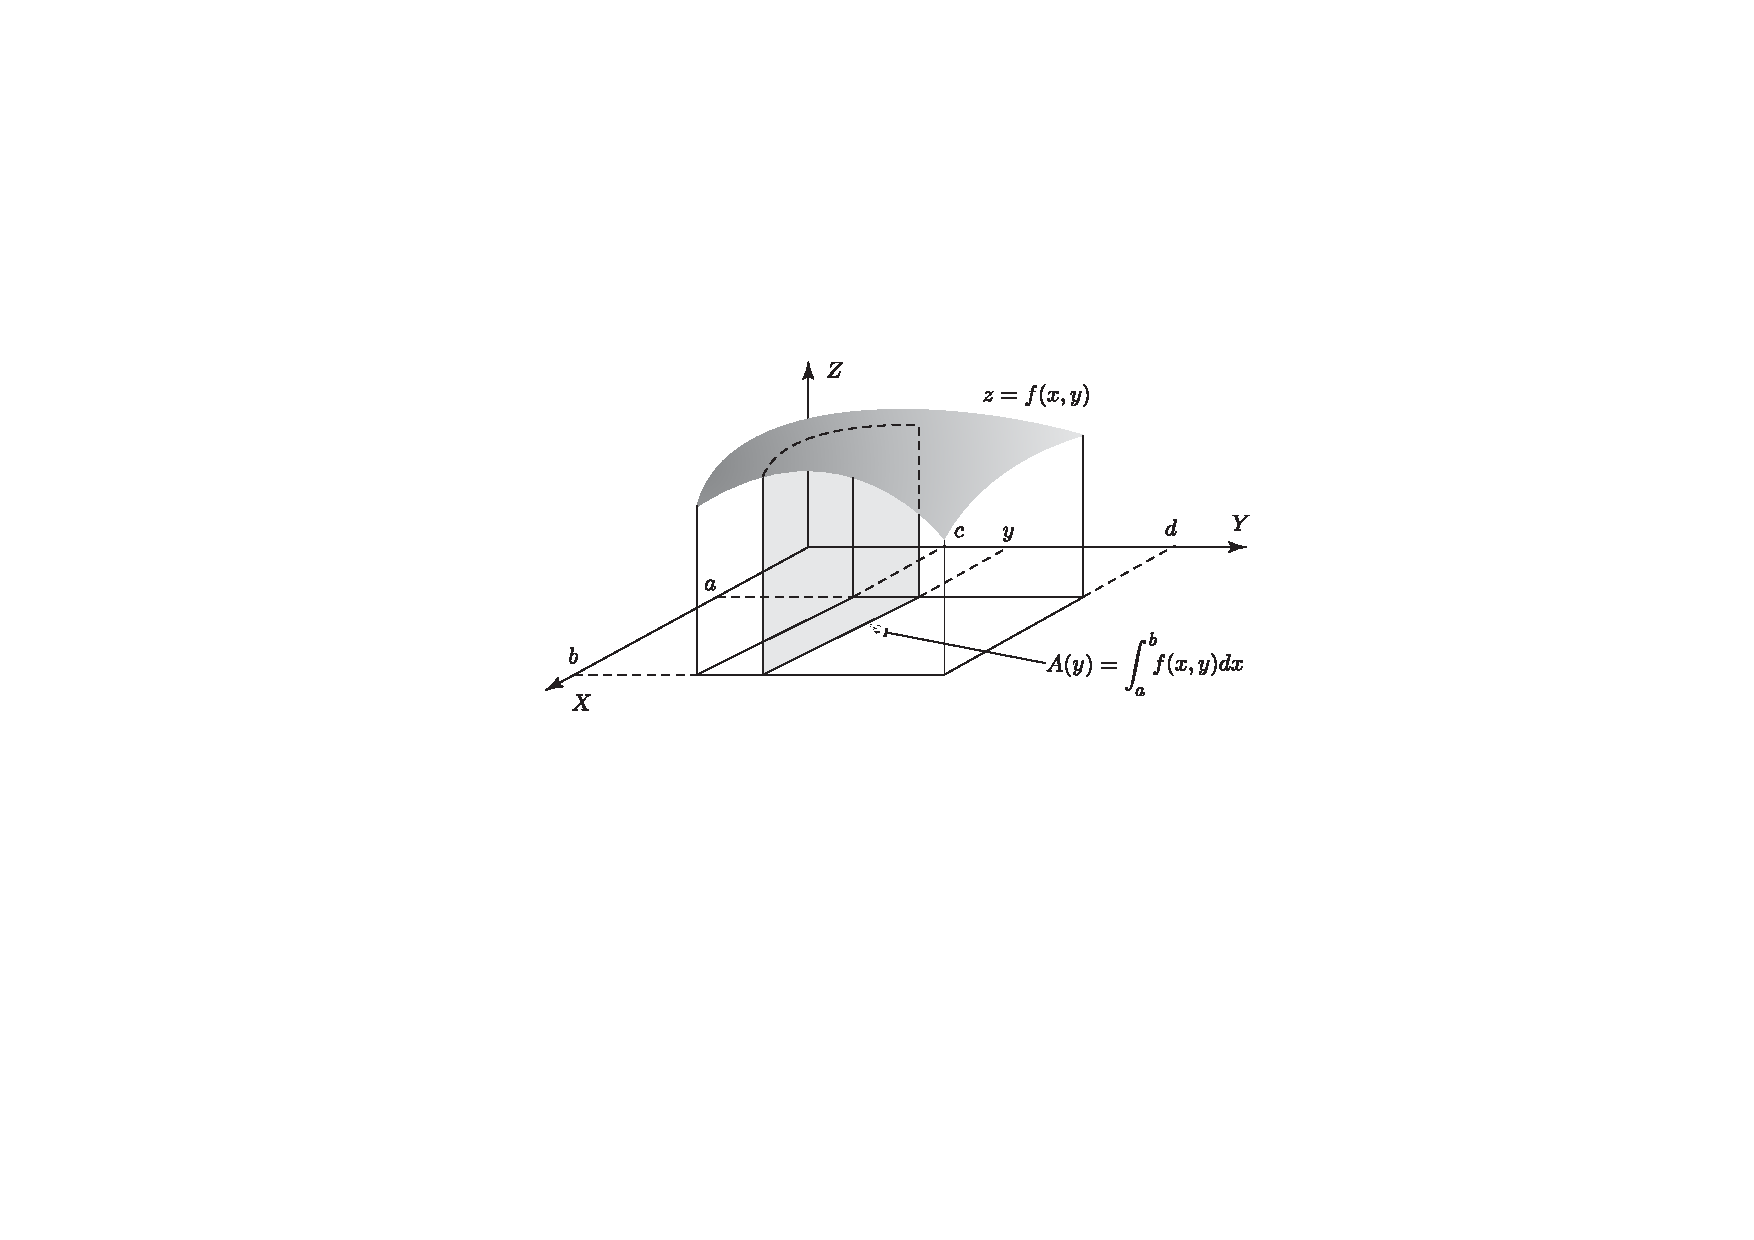
\includegraphics[width=.8\textwidth]{T3/figs/FubIntroY.pdf}\\
$\displaystyle\iint\limits_R f(x,y) = V = \int_c^d A(y)\mathrm dy = \int_c^d \left(\int_a^b f(x,y)\mathrm dx\right)\mathrm dy$
\end{center}
\caption{Justificación del teorema de Fubini usando el cálculo de volúmenes por el método de las secciones.}\label{fig:fub-sec}
\end{figure}
\end{latexonly}

\begin{teorema}[de Fubini]
Sea $f\colon R\subset\mathbb{R}^2\to \mathbb{R}$ un campo escalar integrable en el rectángulo $R=[a,b]\times[c,d]$.
Entonces:
\[
\iint\limits_R f(x,y)\mathrm dx \mathrm dy
=\int_{a}^{b}\left(\int_{c}^{\mathit d}f(x,y)\mathrm dy\right)\mathrm dx
=\int_{c}^{\mathit d}\left(\int_{a}^{b}f(x,y)\mathrm dx\right)\mathrm dy
\]
\end{teorema}
\begin{rawhtml}
&nbsp;
\end{rawhtml}
\begin{ejemplo}
Vamos a calcular la integral $\displaystyle\int_R(2x+y)\mathrm dx\mathrm dy$ con $R=[0,1]\times[0,1]$
%, que estudiamos en la sección anterior haciendo uso de sumas de Riemann.
\begin{align*}
\iint_R(2x+y)\mathrm dx\mathrm dy &= \int_0^1\left(\int_0^1 (2x+y)\mathrm dx\right)\mathrm dy \\
&= \int_0^1 \left[x^2+yx\vphantom{\dfrac12}\right]_{x=0}^1\mathrm dy \\
&= \int_0^1 (1+y)\mathrm dy = \left[y+\frac{y^2}{2}\right]_{y=0}^1=\frac32\tag*{\fej}
\end{align*}
\end{ejemplo}

Como podemos ver en las figuras de la página~\pageref{fig:fub-sec}, las igualdades dadas por el Teorema de Fubini se pueden obtener como consecuencia del método de las secciones para el cálculo de un volumen por el método de las secciones.
\begin{rawhtml}
<div class="center">
<img src="./T3/figuras/Leccion34-3-FubIntroX.svg" width="450">
</div>
<div class="center">
<img src="./T3/figuras/Leccion34-4-FubIntroY.svg" width="450">
</div>
\end{rawhtml}


Naturalmente, trabajar con dominios rectangulares es una restricción demasiado fuerte;
el siguiente resultado introduce la herramienta para trabajar con campos en cualquier dominio.
%
\begin{teorema}\label{th:barf}
Sea $D$ un subconjunto acotado de $\mathbb{R}^2$ y sea $f$ un campo escalar continuo y acotado en $D$. Sea $R$ un rectángulo tal que $D\subset R$ y consideremos el campo
\[
\bar{f}(x,y)=\begin{cases}
f(x,y) & \text{ si } (x,y)\in D\\
0 & \text{ si } (x,y)\in R\smallsetminus D
\end{cases}
\]
Entonces, el campo $\bar f$ es integrable en $R$ y su integral se toma como definición de la integral de $f$ en $D$:
\[
\iint\limits_D f(x,y)\,\mathrm dx\,\mathrm dy \stackrel{(\mathrm{def.})}{=} \iint\limits_R \bar{f}(x,y)\,\mathrm dx\,\mathrm dy
\]
\end{teorema}
\begin{rawhtml}
&nbsp;
\end{rawhtml}
\begin{ejemplo}
Supongamos que $\mathit D\subset\mathbb{R}^2$ está limitado por los grafos de las funciones
$\varphi_1\colon [a,b]\to\mathbb{R}$ y $\varphi_2\colon [a,b]\to\mathbb{R}$ tal y como se muestra en la
figura~\ref{fig:fub}, entonces, considerando la función $\bar{f}$ definida en el
teorema anterior:
\begin{rawhtml}
<div class="center">
<img src="./T3/figuras/Leccion34-5-Fub2.svg" width="300">
</div>
\end{rawhtml}
\begin{align*}
\iint\limits_{\mathit D} f(x,y)\mathrm dx\,\mathrm dy & 
=\int_a^b\left(\int_c^{\mathit d}\bar{f}(x,y)\mathrm dy\right)\mathrm dx\\
& =\int_a^b\left(\int_c^{\varphi_1(x)}0\cdot \mathrm dy+
\int_{\varphi_1(x)}^{\varphi_2(x)}f(x,y) \mathrm dy+\int_{\varphi_2(x)}^{\mathit d}0\cdot \mathrm dy\right)\mathrm dx \\
& =\int_a^b\left(\int_{\varphi_1(x)}^{\varphi_2(x)}f(x,y)\mathrm dy\right)\mathrm dx
\end{align*}
%
\begin{latexonly}
\begin{figure}
\begin{center}
\includegraphics{T3/figs/Fub2.pdf}\\
\end{center}
\caption{Región limitada por dos grafos.}\label{fig:fub}
\end{figure}
\end{latexonly}
%
Por ejemplo, podemos calcular el volumen de la cuña que vimos en un ejemplo anterior, que se obtenía cortando un tronco (cilíndrico) de radio 2 dm dando dos cortes con una sierra mecánica que llegan hasta el centro del
tronco; uno de los cortes se hace perpendicular y el otro formando un ángulo de
$30^\circ$ con  el primero:
\begin{latexonly}
\begin{center}
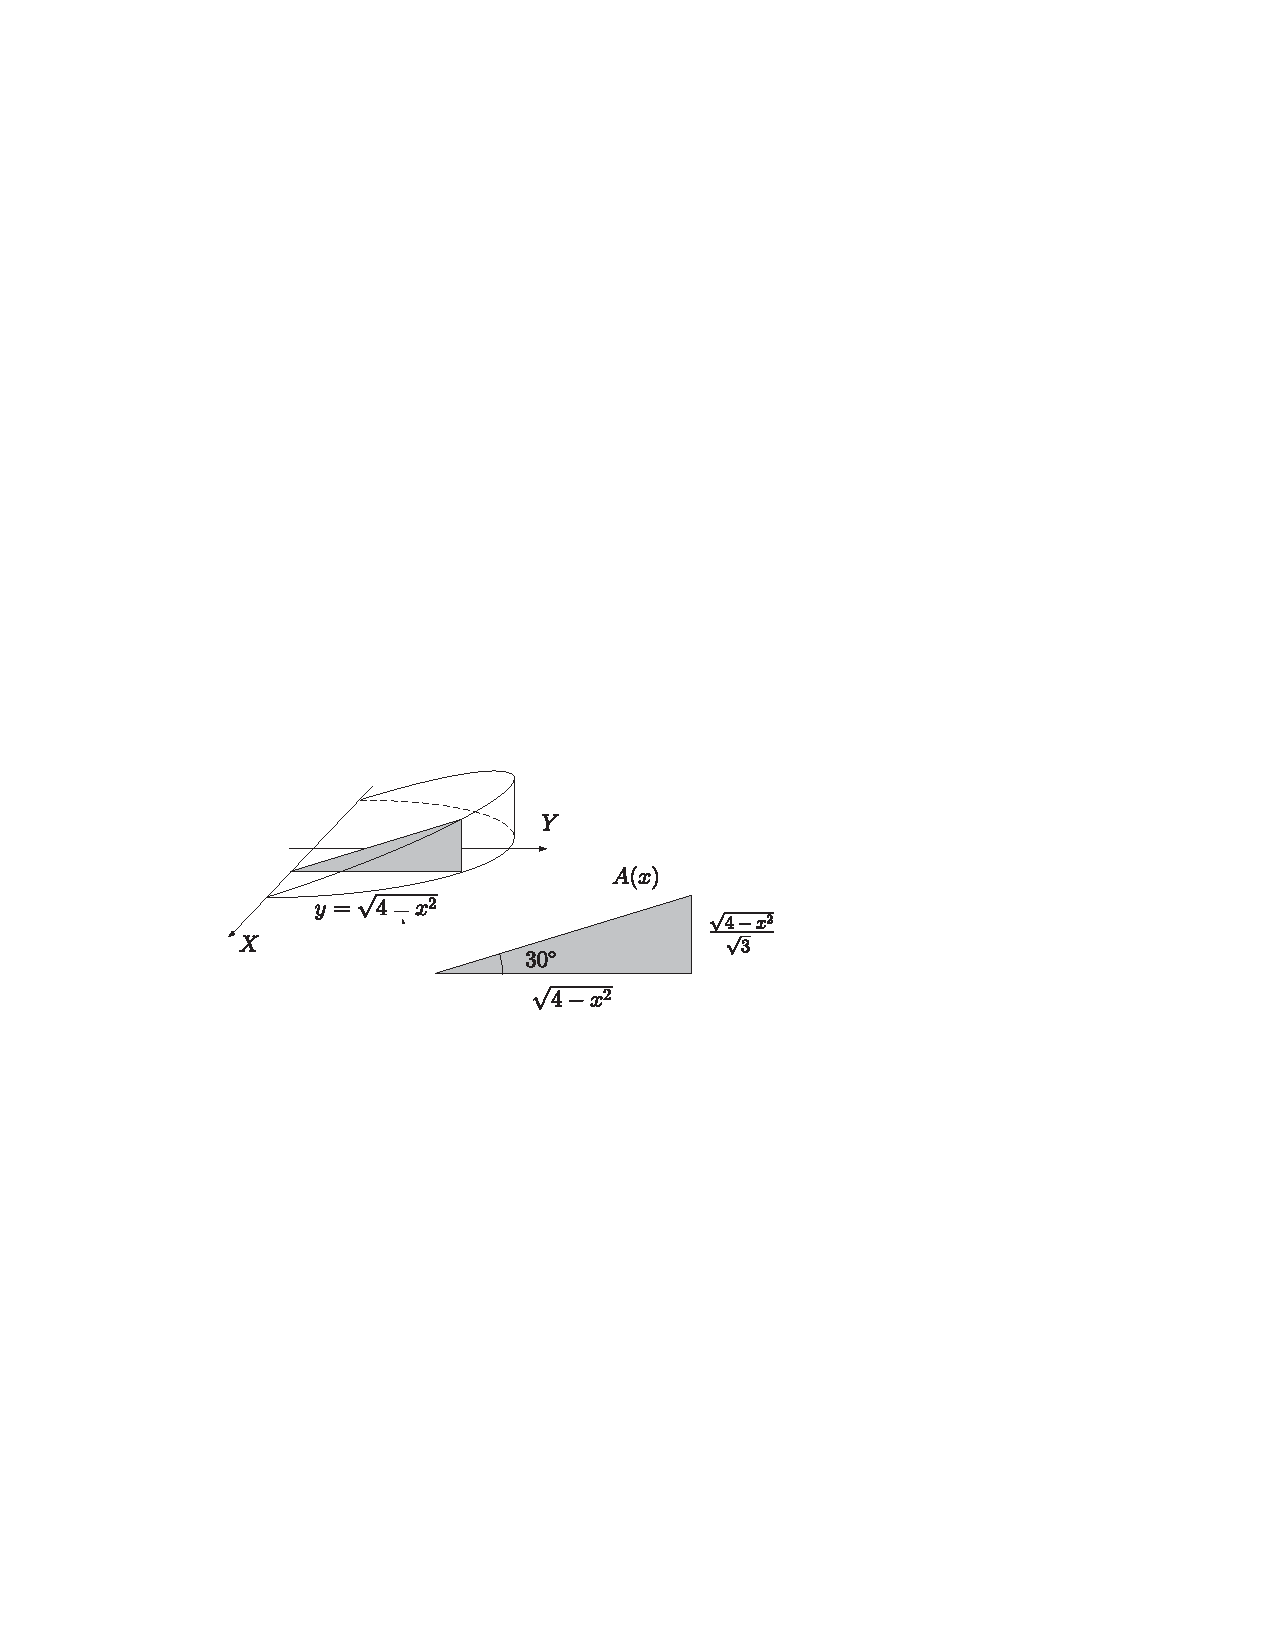
\includegraphics{T3/figs/cunna.pdf}
\end{center}
\end{latexonly}
\begin{rawhtml}
<div class="center">
<img src="./T3/figuras/Leccion33-8-cunna.svg" width="450">
</div>
\end{rawhtml}
Ahora, utilizando una integral doble, la cuña es la región que queda entre el grafo del campo $f(x,y)=\dfrac{y}{\sqrt3}$ y el plano $OX$ en el dominio $\mathit D$ definido por $-2\le x\le 2$, $0\le y \le\sqrt{4-x^2}$.
\begin{align*}
V=&\iint_{\mathit D} \frac{y}{\sqrt3}\,\mathrm dx\,\mathrm dy 
= \int_{-2}^2 \left(\int_0^{\sqrt{4-x^2}} \frac{y}{\sqrt3}\,\mathrm dy\right)\mathrm dx \\
=&\int_{-2}^2 \left[\dfrac{y^2}{2\sqrt3} \right]_0^{\sqrt{4-x^2}}\mathrm dx
= \dfrac{1}{2\sqrt3} \int_{-2}^2  (4-x^2)\mathrm dx\\
= &\dfrac{1}{2\sqrt3} \left[4x-\dfrac{x^3}3\right]_{-2}^2 = \dfrac{16}9\sqrt3\tag*{\fej}
\end{align*}
\end{ejemplo}

Los siguientes resultados establecen varias propiedades de la integral doble.
%
\begin{teorema}
Consideremos un campo escalar $f\colon \mathit{D}\subset\mathbb{R}^2\to \mathbb{R}$ y
supongamos que $f$ es positivo y acotado en $\mathit{D}$.
Entonces, la integral $\int_{\mathit{D}} f(x,y)$ es el valor del volumen del sólido comprendido entre el grafo de $f$ en $\mathit{D}$ y el plano $XY$.
\end{teorema}

Si en este teorema consideramos la función constante $f(x,y)=1$, obtenemos la siguiente consecuencia.

\begin{corolario}\label{cor:areaplana}
$\displaystyle\iint_{\mathit{D}}\,\mathrm dx\,\mathrm dy$ es el valor del área de la región $\mathit D$.
\end{corolario}

La integral doble, también verifica las propiedades de linealidad y de aditividad.

\begin{teorema} Sean $f$ y $g$ campos escalares integrables sobre $\mathit D\subset\mathbb{R}^2$ y
$c,k\in\mathbb{R}$.
\begin{enumerate}
\item Linealidad:
\[\displaystyle\iint\limits_{\mathit D} (c\cdot f(x,y)+k\cdot g(x,y))\,\mathrm dx\,\mathrm dy = c\cdot\Bigg(\iint\limits_{\mathit D} f(x,y)\,\mathrm dx\,\mathrm dy\Bigg)+k\cdot\Bigg(\iint\limits_{\mathit D} g(x,y)\,\mathrm dx\,\mathrm dy\Bigg)
\]
\item Aditividad: Si ${\mathit D}=D_1\cup D_2$ y $\textrm{Área}(D_1\cap D_2) = 0$,
\[
\iint\limits_{\mathit D} f\,\mathrm dx\,\mathrm dy = \Bigg(\iint\limits_{D_1} f(x,y)\,\mathrm dx\,\mathrm dy\Bigg)+\Bigg(\iint\limits_{D_2} f(x,y)\,\mathrm dx\,\mathrm dy\Bigg)
\]
\end{enumerate}
\end{teorema}

\vspace{2em}

\subsection{Teorema de cambio de variable}

El teorema de Fubini es la herramienta fundamental para el cálculo de integrales múltiples, sin embargo, hemos podido observar que su aplicación no es sencilla si la región de integración no es rectangular.
Los cambios de variable nos van a permitir utilizar descripciones más simples de una región. Por ejemplo, mientras que un círculo de radio $a$ centrado en $(0,0)$ en coordenadas cartesianas se describe por $-\sqrt{a^2-x^2}\le y\le \sqrt{a^2-x^2}$, $-a\le x\le a$, en coordenadas polares se describe simplemente por $0\le r\le a$, $0\le \theta\le 2\pi$.
%
\begin{latexonly}
\begin{figure}
\begin{center}
\begin{tikzpicture}[x=1.3em,y=1.3em]
\pgfsetlinewidth{.5pt}
\pgfsetcolor{gray}
\pgfpathgrid[step={\pgfpointxy{1.0472}{1}}]%
{\pgfpointxy{-3}{5}}{\pgfpointxy{3.3}{8}}
\pgfusepath{stroke}
\pgfsetcolor{black}
\draw[-stealth] (-3.2,5) -- (4,5) node[right] {$\Theta$}; 
\draw[-stealth] (-3,4.8) -- (-3,8.3) node[above] {$R$};
\draw (-3,8) node[left] {$a$};
\draw (3.6,5) node[above] {\small $2\pi$};
\draw[-stealth] (-3.3,0) -- (3.3,0) node[right] {$X$}; 
\draw[-stealth] (0,-3.1) -- (0,3.2) node[above] {$Y$};
\draw[thin] (0,0) circle (3);
\foreach \radio in {1,2}
\draw[very thin,color=gray] (0,0) circle (\radio);
%
\foreach \angulo in {15,45,60,75,105,120,135,150,165,180,%
195,210,225,240,255,270,285,300,315,330,345}
\draw[very thin,color=gray] (0,0) -- (\angulo:3.2);
\draw (11,6.5) node{$\begin{array}{c}
0\le r\le a\\
0\le \theta \le 2\pi
\end{array}$};
\draw[-stealth] (11,5) -- (11,1);
\draw (11,3) node[right]{$T$};
\draw (11,-.2) node{$\begin{array}{c}
-a \le x \le a\\
-\sqrt{a^2-x^2}\le y \le \sqrt{a^2-x^2}
\end{array}$};
\end{tikzpicture}
\end{center}
\caption{Cambio de variable a coordenadas polares.}\label{fig:pol}
\end{figure}
\end{latexonly}
%
Para hacer esta descripción alternativa, hemos usado la aplicación
\[
\boldsymbol{T}(r,\theta) = (r\cos\theta,r\operatorname{sen}\theta)
\]
que convierte las \emph{coordenadas polares} en \emph{coordenadas cartesianas}, según se muestra
en la figura~\ref{fig:pol}.
\begin{rawhtml}
<div class="center">
<img src="./T3/figuras/Leccion34-6.svg" width="500">
</div>
\end{rawhtml}
Esta aplicación tiene su origen e imagen en $\mathbb{R}^2$, es decir, es un \emph{campo vectorial}.
Para poder enunciar el teorema de cambio de variable necesitamos introducir algunos conceptos previos.

\begin{definicion} Un campo vectorial es una aplicación cuyo dominio está contenido en un
espacio $\mathbb{R}^n$ y su imagen lo está en otro espacio $\mathbb{R}^m$; es decir, responde al esquema
$\boldsymbol{f}\colon \mathit D\subset\mathbb{R}^n\to \mathbb{R}^m$. Un campo vectorial está determinado por $m$ campos
escalares: $\boldsymbol{f}=(f_1,\dots ,f_m)$.
\end{definicion}

En el teorema de cambio de variable, utilizaremos campos vectoriales continuos y diferenciables, es decir, sus componentes son campos escalares continuos y diferenciables.
La \emph{diferencial} de estos campos se puede estudiar formalmente siguiendo un esquema similar al utilizado para los campos escalares, llegando a la conclusión de que la matriz de esta aplicación lineal se puede expresar a partir de los gradientes de sus componentes según establece la siguiente definición.
Los detalles de estas comprobaciones quedan fuera de los objetivos del curso y de las necesidades de este tema.
%
\begin{definicion}
Si $\boldsymbol{f}=(f_1,\dots,f_m)$ es diferenciable en $\boldsymbol{a}\in \mathrm{Dom}(f)$, llamamos \emph{matriz jacobiana} de $\boldsymbol{f}$ en $\boldsymbol{a}$ a la matriz:
\[
J\boldsymbol{f}(a)=\left(\begin{array}{cccc}
\dfrac{\partial f_1}{\partial x_1}(\boldsymbol{a}) &
\dfrac{\partial f_1}{\partial x_2}(\boldsymbol{a}) & \dots &
\dfrac{\partial f_1}{\partial x_n}(\boldsymbol{a})\\
\dfrac{\partial f_2}{\partial x_1}(\boldsymbol{a}) & 
\dfrac{\partial f_2}{\partial x_2}(\boldsymbol{a}) & \dots & 
\dfrac{\partial f_2}{\partial x_n}(\boldsymbol{a})\\
\vdots & \vdots & \ddots &\vdots \\
\dfrac{\partial f_m}{\partial x_1}(\boldsymbol{a}) & 
\dfrac{\partial f_m}{\partial x_2}(\boldsymbol{a}) & \dots & 
\dfrac{\partial f_m}{\partial x_n}(\boldsymbol{a})
\end{array}\right)_{m\times n}
=\left(\begin{array}{c}
\nabla f_1(\boldsymbol{a})\\
\nabla f_2(\boldsymbol{a})\\
\vdots \\
\nabla f_m(\boldsymbol{a})
\end{array}\right)
\]
\end{definicion}
\begin{rawhtml}
&nbsp;
\end{rawhtml}
\begin{ejemplo}
Vamos a calcular la matriz jacobiana del campo vectorial
\begin{align*}
\boldsymbol f(x,y,z) & =
(3x^2-y,2xz-3y,x-yz^2) \\
J\boldsymbol{f}(x,y,z) & =
\begin{pmatrix}
6x & -1 & 0 \\
2z & -3 & 2x \\
1 & -z^2 & -2yz
\end{pmatrix}\tag*{\fej}
\end{align*}
\end{ejemplo}
Ya tenemos los elementos necesarios para enunciar el teorema de cambio de variable.
%
\begin{teorema} Sea $F\colon \boldsymbol{T}(\mathit D)\subset\mathbb{R}^2\to\mathbb{R}$ un campo escalar continuo, siendo $\mathit D$ cerrado y acotado. Sea $\boldsymbol{T}\colon\mathit D\subset\mathbb{R}^2\to\mathbb{R}^2$ un campo vectorial biyectivo, salvo en un subconjunto de área nula, diferenciable y con las derivadas parciales continuas.
Entonces:
\[
\iint\limits_{\boldsymbol{T}(\mathit D)} F = \iint\limits_{\mathit D} (F\circ \boldsymbol{T})|\det(J\boldsymbol{T})|
\]
\end{teorema}
%
Mientras que para las integrales de una variable, este teorema se utiliza
fundamentalmente para el cálculo de primitivas para simplificar la función a integrar, en la integración múltiple lo utilizaremos fundamentalmente para describir de forma más sencilla la región de integración.

\begin{ejemplo}
Hemos mostrado más arriba el cambio a coordenadas polares:
\[
\boldsymbol{T}(r,\theta) = (r\cos\theta,r\operatorname{sen}\theta)
\]
Veamos como se transforma una integral al aplicar este cambio de variables.
En primer lugar, calculamos el jacobiano de $\boldsymbol{T}$:
\[
J\boldsymbol{T}(r,\theta)=\left(\begin{array}{cc}
\cos\theta & -r\operatorname{sen}\theta\\
\operatorname{sen}\theta & r\cos\theta
\end{array}
\right)
\]
Por lo tanto, el valor absoluto del determinante es: $|\det(J\boldsymbol{T}(r,\theta))| = |r|$;
y la fórmula de cambio de variable queda:
\[
\iint\limits_{\boldsymbol{T}(\mathit D)} F(x,y)\mathrm dx\,\mathrm dy = \iint\limits_{\mathit D} F(r\cos\theta,r\operatorname{sen}\theta)|r|dr\,d\theta
\]
En la integral de la izquierda, $\boldsymbol{T}(\mathit D)$ representa a la región de integración descrita en coordenadas cartesianas, mientras que $\mathit D$, en la integral de la derecha, representa a la misma región pero descrita en coordenadas polares.\fej
\end{ejemplo}
\begin{rawhtml}
&nbsp;
\end{rawhtml}
\begin{ejemplo}\label{ej:reg-paras}
Calculemos la integral $\displaystyle\iint_{D} xy\,\mathrm dx\mathrm dy$ en donde 
$D$ es la región delimitada por las parábolas,
$y=x^2+4, y=x^2, y=6-x^2, y=12-x^2$, según se muestra en la figura~\ref{fig:reg-paras}
\begin{rawhtml}
<div class="center">
<img src="./T3/figuras/Leccion34-8-region.svg" width="220">
</div>
\end{rawhtml}
\begin{latexonly}
\begin{figure}
\begin{center}
\includegraphics{T3/figs/region.pdf}
\end{center}
\caption{Región de integración en el ejemplo~\ref{ej:reg-paras}.}\label{fig:reg-paras}
\end{figure}
\end{latexonly}
En este caso, cada par $(u,v)$ tal que $u\in[6,12]$, $v\in[0,4]$, determina un único punto de la región, determinado por las siguientes ecuaciones
\[
y=x^2+v,\quad  y=u-x^2
\]
Esto permite obtener un cambio de variable de $[6,12]\times [0,4]$ en $D$:
\[
x=\sqrt{\frac12(u-v)},\qquad y=\frac12(u+v)
\]
Utilizamos entonces el cambio $\boldsymbol{T}(u,v)=(\sqrt{\frac12(u-v)},\frac12(u+v))$, para calcular la integral propuesta
\[
\mathrm{Det}(J\boldsymbol{T}(u,v))=\left|\begin{matrix}
\dfrac{\sqrt2}{4\sqrt{u-v}} & \dfrac{-\sqrt2}{4\sqrt{u-v}} \\
\dfrac12 & \dfrac12
\end{matrix}\right| = \dfrac{\sqrt2}{4\sqrt{u-v}}
\]
\begin{multline*}
\iint\limits_{D} xy\,\mathrm dx\mathrm dy =
\iint\limits_{T^{-1}(D)} \dfrac{\sqrt{u-v}(u+v)}{2\sqrt2}\dfrac{\sqrt2}{4\sqrt{u-v}}\mathrm du\,\mathrm dv\\ =
\dfrac{1}{8}\int_0^4\int_6^{12}(u+v)\mathrm du\,\mathrm dv
=\dfrac18\int_0^4\left[\dfrac{u^2}{2}+vu\right]_{u=6}^{12}\mathrm dv\\
=\dfrac18\int_0^4(54+6v)\mathrm dv
=\dfrac18\left[54v+3v^2\vphantom{\dfrac12}\right]_{v=0}^{4}\mathrm dv 
= 33\tag*{\fej}
\end{multline*}
\end{ejemplo}

%\subsection{Aplicaciones}

%Tal y como ocurre con las funciones de variable real, las aplicaciones de la integral doble no se reducen al cálculo de volúmenes. Son múltiples las magnitudes físicas, matemáticas y de otras áreas que pueden ser modeladas y calculadas con este tipo de integrales. A modo de ejemplo, mostramos dos aplicaciones geométricas.

\subsection{Áreas de regiones planas}

Según hemos visto anteriormente, la integral doble nos da una forma sencilla de expresar el área de una región plana arbitraria:
\[
\mathrm{\acute{A}rea}(\mathit D)=\iint\limits_{\mathit D} \mathrm dx\mathrm dy,
\]
El uso de las técnicas presentadas en las secciones anteriores nos permitirá abordar el cálculo del área de regiones cuyas representaciones como integrales de una variable sería más compleja.

\begin{ejemplo}
Calculemos el área de la región interior a la elipse $\dfrac{x^2}{a^2}+\dfrac{y^2}{b^2}=1$.
%\[
%\mathrm{\acute{A}rea}(D)=\int\limits_D \mathrm dx\mathrm dy.
%\]
Podemos plantear la integral en la región elíptica aplicando directamente el teorema de Fubini, pero las primitivas resultantes no serán sencillas.
Es mejor utilizar un cambio de variable, que podemos intuir fácilmente si recordamos la parametrización de la elipse que estudiamos en el tema~2:
\[
\frac{x}a =r \cos t,\qquad \frac{y}b=r\operatorname{sen} t,\quad r\in[0,1],\quad t\in[0,2\pi].
\]
Obsérvese que este cambio no es el cambio a coordenadas polares; de hecho, el uso de coordenadas polares sobre regiones elípticas conduce, por lo general, a primitivas más complejas.

Por lo tanto:
\begin{align*}
\boldsymbol{T}(r,t) &= (ar\cos t,br\operatorname{sen} t) \\
J\boldsymbol{T}(r,t) &=
\begin{pmatrix}
a\cos t & -ar\operatorname{sen} t \\
b\operatorname{sen} t & br\cos t
\end{pmatrix} \\
|\mathrm{Det}(J\boldsymbol{T}(r,t))| & = rab \\
\mathrm{\acute{A}rea}(\mathit D)&=\iint\limits_{\mathit D} \mathrm dx\mathrm dy=\int_0^{2\pi}\int_0^1 abr\,dr\,\mathrm dt =\pi ab\tag*{\fej}
\end{align*}
\end{ejemplo}


%
%\paragraph{Áreas de grafos.} Si $f$ es un campo escalar continuo con parciales continuas en un dominio~$\mathit D$, entonces el área de la superficie de su grafo sobre el dominio $\mathit D$ es
%\[
%\int\limits_{\mathit D} \sqrt{1+\Big(\dfrac{\partial f}{\partial x}(x,y)\Big)^2+
%\Big(\dfrac{\partial f}{\partial y}(x,y)\Big)^2}\,\mathrm dx\,\mathrm dy
%\]
%La expresión del integrando se conoce como \emph{diferencial de superficie} y juega un papel similar al de la diferencial de longitud.
%
%%:Arreglar: Pasar integral de línea a la lección anterior y dejar aquí solo
%% el teorema de Green.

\subsection{Integrales de línea}

Una de las aplicaciones fundamentales de la integral en la física es el cálculo del trabajo que realiza un campo (vectorial) de fuerzas al desplazarse por una curva. 
Esta magnitud se modeliza con lo que se conoce como \emph{integral de línea}, que definimos a continuación.
%
\begin{definicion}
Sea $\boldsymbol{F}=(F_1,F_2)$ un campo vectorial y $\gamma(t)$, $t\in[a,b]$, una curva en $\mathbb{R}^2$ tal que $\gamma'$ es continua en $[a,b]$.
Llamamos \emph{integral de línea de $\boldsymbol{F}$ sobre la curva $C$} o \emph{circulación de $\boldsymbol{F}$ a través de $C$}~a:
\[
\int_C \boldsymbol{F} = 
\int_a^b \boldsymbol{F}(\gamma(t))\cdot\gamma'(t)\,\mathrm dt
= \int_a^b (F_1(x(t),y(t))x'(t)+F_2(x(t),y(t))y'(t))\,\mathrm dt
\]
Si la curva $C$ es cerrada, es decir $\gamma(a)=\gamma(b)$, esta integral se denota:
$\displaystyle\oint_C \boldsymbol{F}$
\end{definicion}
De forma más abreviada, la integral de línea se suele expresar igualmente como sigue:
\[
\int_C \boldsymbol{F} = \int_C F_1(x,y)\mathrm dx+F_2(x,y)\mathrm dy
\]

\begin{latexonly}
\begin{figure}
\begin{center}
\begin{tikzpicture}[x=30em,y=30em]
\draw[domain=0:.1,smooth,variable=\t,-stealth]
plot (2*\t*\t*\t-3*\t*\t+\t,\t-\t*\t);
\draw[domain=.1:.3,smooth,variable=\t,-stealth]
plot (2*\t*\t*\t-3*\t*\t+\t,\t-\t*\t);
\draw[domain=.3:.6,smooth,variable=\t,-stealth]
plot (2*\t*\t*\t-3*\t*\t+\t,\t-\t*\t);
\draw[domain=.6:.9,smooth,variable=\t,-stealth]
plot (2*\t*\t*\t-3*\t*\t+\t,\t-\t*\t);
\draw[domain=.9:1,smooth,variable=\t]
plot (2*\t*\t*\t-3*\t*\t+\t,\t-\t*\t);
% Ejes
\draw[-stealth] (-.16,0) -- (.16,0) node[right] {$X$}; 
\draw[-stealth] (0,-.01) -- (0,.3) node[right] {$Y$};;
\end{tikzpicture}
\end{center}
\caption{Curva de los ejemplos~\ref{ej:int-lin} y~\ref{ej:area-green}.}\label{fig:ej-int-lin}
\end{figure}
\end{latexonly}
\begin{ejemplo}\label{ej:int-lin}
Consideremos el campo $\boldsymbol F(x,y)=\Big(\dfrac{x}{y},\dfrac{y}x\Big)$ y la curva cerrada $C$ determinada por la parametrización
$\gamma(t)=(2t^3-3t^2+t,t-t^2)$, $t\in[0,1]$ (ver figura~\ref{fig:ej-int-lin}).
\begin{rawhtml}
<div class="center">
<img src="./T3/figuras/Leccion34-9.svg" width="250">
</div>
\end{rawhtml}
\begin{multline*}
\oint_{C} \boldsymbol{F} = 
\int_0^1 \boldsymbol{F}(\gamma(t))\cdot\gamma'(t)\,\mathrm dt
= \int_0^1 (F_1(x(t),y(t))x'(t)+F_2(x(t),y(t))y'(t))\,\mathrm dt =\\
= \int_0^1 \left(\frac{x(t)}{y(t)}x'(t)+\frac{y(t)}{x(t)}y'(t)\right)\,\mathrm dt =\\
= \int_0^1 \left(\frac{t(t-1)(2t-1)}{-t(t-1)}(6t^2-6t+1)+
\frac{-t(t-1)}{t(t-1)(2t-1)}(1-2t)\right)\,\mathrm dt =\\
= \int_0^1 \big(-(2t-1)(6t^2-6t+1)+1\big)\,\mathrm dt =\\
= \int_0^1 (-12t^3+18t^2-8t+2)\,\mathrm dt =\\
= \left[-3t^4+6t^3-4t^2+2t\right]_0^1=-3+6-4+2=1\tag*{\fej}
\end{multline*}
\end{ejemplo}

Las integrales de línea y las integrales dobles están relacionadas por el teorema de Green, que enunciamos a continuación.
%
\begin{teorema}[de Green]\label{th:green}
Sea $C$ es una curva regular a trozos, cerrada y simple de $\mathbb{R}^2$ recorrida de tal forma que el interior de la curva queda a la izquierda,~$\mathit D$ la región interior de esta curva y
$\boldsymbol{F}\colon \mathit D\subset\mathbb{R}^2\to\mathbb{R}^2$ un campo vectorial continuo y con parciales continuas en~$\mathit D$.
Entonces
\[
\oint_C \boldsymbol{F}  =  \int\limits_{\mathit D} \Big(\dfrac{\partial F_2}{\partial x}(x,y) - \dfrac{\partial F_1}{\partial y}(x,y)\Big)\,\mathrm dx\,\mathrm dy
\]
\end{teorema}

\begin{latexonly}
\begin{figure}
\begin{center}
\begin{tikzpicture}[x=6em,y=6em]
\draw[very thick,domain=0:.3,smooth,variable=\t,-stealth]
plot (1-\t,-\t*\t+2*\t);
\draw[very thick,domain=.3:.8,smooth,variable=\t,-stealth]
plot (1-\t,-\t*\t+2*\t);
\draw[very thick,domain=.8:1.6,smooth,variable=\t,-stealth]
plot (1-\t,-\t*\t+2*\t);
\draw[very thick,domain=1.6:2,smooth,variable=\t,-stealth]
plot (1-\t,-\t*\t+2*\t);
\draw[very thick,-stealth] (-1,0)--(-.3,0);
\draw[very thick,-stealth] (-.3,0)--(.6,0);
\draw[very thick,-stealth] (.6,0)--(1,0);
\draw[<-] (.51,.76)--(.7,1) node[right]{$y=1-x^2$};
\draw (-1,0) node[below]{$-1$};
\draw (1,0) node[below]{$1$};
% Ejes
\draw[-stealth] (-1.2,0) -- (1.2,0) node[right] {$X$}; 
\draw[-stealth] (0,-.1) -- (0,1.2) node[right] {$Y$};;
\end{tikzpicture}
\end{center}
\caption{Curva del ejemplo~\ref{ej:green}.}\label{fig:ej-green}
\end{figure}
\end{latexonly}
\begin{ejemplo}\label{ej:green}
Vamos a calcular la integral del campo $\boldsymbol F(x,y)=(y^2,x^2)$ sobre la curva cerrada $C$ que aparece en la figura~\ref{fig:ej-green}; 
\begin{rawhtml}
<div class="center">
<img src="./T3/figuras/Leccion34-10.svg" width="300">
</div>
\end{rawhtml}
esta curva está formada por el segmento que une los puntos $(-1,0)$ y $(1,0)$ y el segmento de la parábola $y=1-x^2$ que va de $(1,0)$ a $(-1,0)$.
Dado que vamos a utilizar el teorema de Green, no es necesario obtener una parametrización.
Si $\mathit{D}$ es la región encerrada por la curva: 
\begin{multline*}
\oint_{C} \boldsymbol{F} = 
\oint_{C} y^2\,\mathrm dx + x^2\,\mathrm dy =
\iint\limits_{\mathit D} (2x-2y)\,\mathrm dx\,\mathrm dy =\\
=\int_{-1}^1 \int_0^{1-x^2} (2x-2y)\,\mathrm dy\,\mathrm dx =
\int_{-1}^1 \left[2xy-y^2\right]_0^{y=1-x^2}\,\mathrm dx =\\
=\int_{-1}^1 2x(1-x^2)-(1-x^2)^2\,\mathrm dx =
\int_{-1}^1 (-x^4-2x^3+2x^2+2x-1)\,\mathrm dx =\\
=\left[-\frac15x^5-\frac12x^4+\frac23x^3+x^2-x\right]_{-1}^1  =\\
=(-\frac15-\frac12+\frac23+1-1)-(\frac15-\frac12-\frac23+1+1) = \frac{-16}{15}\tag*{\fej}
\end{multline*}
\end{ejemplo}

Si $C$ es una curva cerrada y $D$ es la región del plano que encierra, entonces, por el teorema de Green
\[
\oint_{C} -y\,\mathrm dx + x\,\mathrm dy = \iint\limits_{\mathit D} (1-(-1))\,\mathrm dx\,\mathrm dy )= 
2\iint\limits_{\mathit D} \mathrm dx\,\mathrm dy = 2\text{Área}(D)
\]
Hemos considerado que la curva se está recorriendo en sentido positivo, es decir, de tal forma que el interior queda a la izquierda.
Si la curva se recorre en sentido contrario, el valor de la integral será negativo, aunque su valor absoluto coincidirá igualmente con el área.
Este razonamiento demuestra el siguiente corolario.

\begin{corolario}\label{cor:areacurva}
Si $C$ es una curva regular, cerrada y simple, entonces el área de la región encerrada por $C$ es
\[
A= \frac12\left|\oint_C -y\,\mathrm dx+x\,\mathrm dy\right|
\]
\end{corolario}
\begin{rawhtml}
&nbsp;
\end{rawhtml}
\begin{ejemplo}\label{ej:area-green}
Vamos a calcular el área de la región  encerrada por la curva $C$ determinada por la parametrización $\gamma(t)=(2t^3-3t^2+t,t-t^2)$, $t\in[0,1]$ (ver figura~\ref{fig:ej-int-lin}).
\begin{multline*}
\text{Área}=\frac12\oint_{C} -y\,\mathrm dx+x\,\mathrm dy =\\
= \int_0^1 \frac12\big(-(t-t^2)(6t^2-6t+1)+(2t^3-3t^2+t)(1-2t)\big)\,\mathrm dt =\\
= \int_0^1 (t^4-2t^3+t^2)\,\mathrm dt 
= \left[\frac15t^5-\frac12t^4+\frac13t^3\right]_0^1=\frac15-\frac12+\frac13=\frac1{30}\tag*{\fej}
\end{multline*}
\end{ejemplo}


%    \newpage
%    \thispagestyle{empty}
%    
%    \ 
%    
%    \vfill
%    \begin{center}
%    (Esta página se ha dejado intencionalmente en blanco)
%    \end{center}

\newpage

%%%%%%%%%%%%%%%%%%%%%%%%%%%%%%%%%%%%%%%%%%%%%%%%%%%%%%%%%%%%%%%%%%%%%%%%%%%%%%%%%%%%
\section*{Relación de ejercicios \thechapter.1}
%%%%%%%%%%%%%%%%%%%%%%%%%%%%%%%%%%%%%%%%%%%%%%%%%%%%%%%%%%%%%%%%%%%%%%%%%%%%%%%%%%%%

\pagestyle{relaciones}


\begin{enumerate}


\item Las expresiones $\dfrac{1}{x}$ y $\dfrac{2}{2x}$ son iguales, sin embargo, si calculamos la integral (inmediata) de cada una de ellas, obtenemos los siguientes resultados:
\[
\displaystyle\int\frac{1}{x}\,\mathrm dx=\log |x|+C \qquad\text{ y }\qquad \displaystyle\int\frac{2}{2x}\,\mathrm dx=\log|2x| + C
\] 
¿Son esos dos resultados realmente distintos?


\item Calcule las siguientes integrales observando que son inmediatas:

\setcontadoralph
\begin{center}
\begin{tabular}{l@{\qquad\quad}l}
\nitem $\displaystyle\int(4x^3-3x^2+\dfrac{1}{2}x-\pi)\,\mathrm dx$ &
\nitem $\displaystyle\int\sqrt[3]{x^2}\,\mathrm dx$ \\
\nitem $\displaystyle\int\cos x\operatorname{sen}^3 x\,\mathrm dx$ &
\nitem $\displaystyle\int x\operatorname{sen} x^2\,\mathrm dx$
\end{tabular}
\end{center}

\item
\begin{enumerate}
\item
Transforme el polinomio $9x^2-6x+2$ usando la técnica de completar cuadrados.
\item
Utilice la expresión anterior para calcular la integral $\displaystyle\int\dfrac{3}{9x^2-6x+2}\mathrm{d}x$
\end{enumerate}


\item
Utilice la descomposición en fracciones simples para calcular la integral
\[
\int\dfrac{x^2+6x+5}{x^3-x^2-x-2}\mathrm{d}x
\]


\item Calcule las siguientes integrales racionales, analizando en primer lugar si son inmediatas:

\setcontadoralph
\begin{centrar}
\nitem $\displaystyle\int\dfrac{x}{4+x^4}\,\mathrm dx$ \hfill
\nitem $\displaystyle\int\dfrac{x^3}{4+x^4}\,\mathrm dx$ \hfill
\nitem $\displaystyle\int\dfrac{x^2}{4+x^4}\,\mathrm dx$
\end{centrar}

\item Calcule las  integrales 
\setcontadoralph
\begin{centrar}
\nitem $\displaystyle\int\operatorname{tg} x\,\mathrm dx$,\hfill
\nitem $\displaystyle\int(\log x)^2\,\mathrm dx$
\end{centrar}
y deduzca a partir de ellas las integrales siguientes:
\begin{centrar}
\nitem $\displaystyle\int e^x\,\operatorname{tg} e^x\,\mathrm dx$,\hfill
\nitem $\displaystyle\int\dfrac{(\log(\operatorname{arctg} x))^2}{1+x^2}\,\mathrm dx$
\end{centrar}


\item Calcule las  integrales siguientes utilizando el método de integración por partes.
\setcontadoralph
\begin{centrar}
\nitem $\displaystyle\int e^{2x}\cos x\,\mathrm dx$ \hfill
\nitem $\displaystyle\int x^5 \operatorname{sen} x^3\,\mathrm dx$
\end{centrar}

\item
Utilice el cambio de variable $t=e^x$ y las fórmulas de derivación vistas en el tema para calcular la integral
\[
\displaystyle\int\dfrac{\text{e}^x\,\mathrm dx}{1-\text{e}^{2x}}
\]

\item Calcule las siguientes integrales teniendo en cuenta que son funciones racionales en seno y coseno y utilizando el cambio más adecuado según lo explicado en la sección~\ref{trig}.
\setcontadoralph
\begin{centrar}
\nitem $\displaystyle\int\operatorname{sen}^3 x\cos^2 x\,\mathrm dx$ \hfill
\nitem $\displaystyle\int\dfrac{\mathrm dx}{1+\cos x}$
\end{centrar}

\item
Calcule la integral $\displaystyle\int \dfrac{\sqrt{1-x}}{1-\sqrt{x}}\,\mathrm dx$ utilizando en primer lugar el cambio de variable $x=\operatorname{sen}^2 t$ y posteriormente el cambio más adecuado según lo explicado en la sección~\ref{trig}.

\item Consideramos la integral $\displaystyle\int\cos^5 x\,\mathrm dx$:
\begin{enumerate}
\item
Calcúlela utilizando la forma compleja de las funciones trigonométricas.
\item
Calcúlela utilizando el cambio de variable $\operatorname{sen} x=t$.
\end{enumerate}


\item
Resuelva las siguientes integrales irracionales.
\setcontadoralph
\begin{centrar}
\nitem $\displaystyle\int\dfrac{x\,\mathrm dx}{\sqrt{5-4x-x^2}}$ \hfill
\nitem $\displaystyle\int(x-3)\sqrt{x^2-6x}\,\mathrm dx$ 
\end{centrar}

\item
Calcule las siguientes integrales prestando especial atención al indicador de la variable ($\mathrm dx$ o $\mathrm dy$) de integración.
\setcontadoralph
\begin{center}
\begin{tabular}{l@{\qquad\qquad}l@{\qquad\qquad}l}
\nitem $\displaystyle\int x\,\mathrm dx$ &
\nitem $\displaystyle\int 2xy^2\,\mathrm dx$ &
\nitem $\displaystyle\int \dfrac{x}{y^2+x^4}\,\mathrm dx$ \\
\nitem $\displaystyle\int x\,\mathrm dy$ &
\nitem $\displaystyle\int 2xy^2\,\mathrm dy$ &
\nitem $\displaystyle\int\dfrac{x}{y^2+x^4}\,\mathrm dy$
\end{tabular}
\end{center}



\end{enumerate}

%%%%%%%%%%%%%%%%%%%%%%%%%%%%%%%%%%%%%%%%%%%%%%%%%%%%%%%%%%%%%%%%%%%%%%%%%%%%%%%%%%%%
\newpage
%%%%%%%%%%%%%%%%%%%%%%%%%%%%%%%%%%%%%%%%%%%%%%%%%%%%%%%%%%%%%%%%%%%%%%%%%%%%%%%%%%%%
\section*{Relación de ejercicios \thechapter.2}
%%%%%%%%%%%%%%%%%%%%%%%%%%%%%%%%%%%%%%%%%%%%%%%%%%%%%%%%%%%%%%%%%%%%%%%%%%%%%%%%%%%%

\pagestyle{relaciones}


\begin{enumerate}

\item Distinga si las siguientes expresiones son ecuaciones diferenciales y determine el tipo (ordinarias o en derivadas parciales) y el orden.
\setcontadoralph
\begin{center}
\begin{tabular}{l@{\qquad\qquad}l}
\nitem $x^2+3y^2=5xy$ &
\nitem $x^2+3y''-5(y')^3=0$ \\
\nitem $1+y+y''+y'''=0$ &
\nitem $xy-y'\operatorname{sen} x=0$ \\
\nitem $x\dfrac{\mathrm dy}{\mathrm dx}-\operatorname{sen} x = \mbox{e}^x$ &
\nitem $5\left(\dfrac{\partial z}{\partial x}\right)^2+xy\dfrac{\partial z}{\partial y}=3xyz$
\end{tabular}
\end{center}


\item Consideremos la ecuación $y'+2y=0$. Se pide:
\begin{enumerate}
\item Estudie la existencia y unicidad de soluciones.
\item Compruebe que la función $y=Ce^{-2x}$ es una solución general.
\item Determine la solución particular que pasa por el punto $(0,3)$.
\end{enumerate}

\item Consideremos la ecuación diferencial $y'=y^2-4$. Se pide
\begin{enumerate}
\item Estudie la existencia y unicidad de soluciones
\item Resuelva la ecuación (variables separables) y obtener la solución general.
\item Calcule la solución particular, si existe, que pasa por $(0,0)$.
\item Calcule la solución particular, si existe, que pasa por $(0,2)$.
\item Calcule la solución particular, si existe, que pasa por $(0,-2)$.
\end{enumerate}

\item
Compruebe que la ecuación $xyy'-\log x=0$ es de variables separables y resuélvala. ¿Alguna solución pasa por el punto $(1,-2)$?


\item
Compruebe que la ecuación $(2x-3y)+(2y-3x)y'=0$ es exacta y resuélvala.  ¿Alguna solución pasa por el punto $(1,-2)$?


\item
Resuelva la ecuación diferencial lineal
$y'+\dfrac{y}{x}=3x+4$ y compruebe la solución.  ¿Alguna solución pasa por el punto $(2,6)$?



\item
Resuelva la ecuación $y'=\dfrac{xy}{x^2-y^2}$ utilizando el cambio de variable $y=x\cdot u$ y compruebe la solución.

\item
Resuelva la ecuación $yy'-2y^2=e^x$ utilizando el cambio de variable $u=y^2$.

\item
Entre los modelos estudiados en el tema, determine qué tipo de ecuación diferencial es cada una de las siguientes:
\setcontadoralph
\begin{center}
\begin{tabular}{l@{\qquad\quad}l}
\nitem $(2+x)y'=3y$ &  %sep
\nitem $y'=\dfrac{3x+2y}{x}$ \\ %lin
\nitem $2\cos(2x-y)-y'\cos(2x-y)=0$ & %exac
\nitem $y'=-2-y+y^2$ \\ %sep
\nitem $(x-1)y'+y=x^2-1$ & %lin
\nitem $y'=\dfrac{y+x-3}{y-x-1}$ \\ %exac
\nitem $y'+2xy=2x$ & %lin
\nitem $e^xyy'=e^{-y}+e^{-2x-y}$ \\ %sep
\nitem $y'+2y=\operatorname{sen} x$ & %lin
\nitem $y^2e^{xy^2} + 2xyy'e^{xy^2}=0$ %exac
\end{tabular}
\end{center}

\end{enumerate}

%%%%%%%%%%%%%%%%%%%%%%%%%%%%%%%%%%%%%%%%%%%%%%%%%%%%%%%%%%%%%%%%%%%%%%%%%%%%%%%%%%%%
\newpage
\thispagestyle{empty}

\ 

\vfill
%\begin{center}
%(Esta página se ha dejado intencionalmente en blanco)
%\end{center}
\newpage

%%%%%%%%%%%%%%%%%%%%%%%%%%%%%%%%%%%%%%%%%%%%%%%%%%%%%%%%%%%%%%%%%%%%%%%%%%%%%%%%%%%%
\section*{Relación de ejercicios \thechapter.3}
%%%%%%%%%%%%%%%%%%%%%%%%%%%%%%%%%%%%%%%%%%%%%%%%%%%%%%%%%%%%%%%%%%%%%%%%%%%%%%%%%%%%

\pagestyle{relaciones}


\begin{enumerate}


\item
Calcule la siguiente integral utilizando el cambio de variable $x=t^2$.
\[
\displaystyle\int_0^{\pi^2/4}\operatorname{sen}\sqrt{x}\,\mathrm dx
\]

\item
Calcule el área de las regiones acotadas delimitadas por las gráficas de las funciones $f(x)=x^4-9x^2+10$ y
$g(x)=x^2+1$.


%Volumen por discos y capas
\item Consideremos la región comprendida entre la curva $y=x^2$ y la recta $y=x+2$.
Dibuje la región y utilice los modelos de la sección~\ref{sec:geom} para calcular los siguientes volúmenes.
\begin{enumerate}
\item Volumen de revolución que se genera al girar la región alrededor del eje $X=2$.
\item Volumen de revolución que se genera al girar la región alrededor del eje $Y=-1$.
\end{enumerate}


%Longitud de un arco en paramétricas
\item Halle la distancia recorrida por un móvil entre los instantes $t=0$ y $t=4$ si su posición viene determinada por las ecuaciones:
$$ x(t)=\frac{t^2}{2},\qquad y(t)=\frac{1}{3}(2t+1)^{3/2} $$


\item
Halle la integral $\displaystyle\iint\limits_R y^3\cos^2x\,\mathrm dx\,\mathrm dy$, en donde
$R=[-1,2]\times [0,2]$

\item
Halle la integral $\displaystyle\iint\limits_R yx^3 e^{x^2y^2}\,\mathrm dx\,\mathrm dy$, en donde
$R=[1,3]\times [1,2]$


\item Dibuje la región sobre la que se integra, intercambie el orden de
integración y evalúe la integral 
\[
\int_0^1\int_x^1 (x-y)^3\,\mathrm dy\,\mathrm dx.
\]

\item Dibuje la región sobre la que se integra, intercambie el orden de
integración y evalúe la integral 
\[
\int_1^4\int_1^{\sqrt{x}} (x^2+y^2)\,\mathrm dy\,\mathrm dx.
\]

\end{enumerate}

\newpage
\thispagestyle{empty}

\ 

\vfill
%\begin{center}
%(Esta página se ha dejado intencionalmente en blanco)
%\end{center}
%%%%%%%%%%%%%%%%%%%%%%%%%%%%%%%%%%%%%%%%%%%%%%%%%%%%%%%%%%%%%%%%%%%%%%%%%%%%%%%%%%%%
\newpage
%%%%%%%%%%%%%%%%%%%%%%%%%%%%%%%%%%%%%%%%%%%%%%%%%%%%%%%%%%%%%%%%%%%%%%%%%%%%%%%%%%%%
\section*{Relación de ejercicios \thechapter.4}
%%%%%%%%%%%%%%%%%%%%%%%%%%%%%%%%%%%%%%%%%%%%%%%%%%%%%%%%%%%%%%%%%%%%%%%%%%%%%%%%%%%%

\pagestyle{relaciones}


\begin{enumerate}
\item
Consideramos la región $R$ delimitada por las rectas $y=x+1$, $y=x-3$, $y=4-x$, $y=3-x$.
Utilizar el teorema de cambio de variable para expresar la integral respecto de las variables $u$ y $v$ tales que $y=x+u$, $y=v-x$ y calcularla
\[
\iint\limits_R (y-2x)\,\mathrm dx\,\mathrm dy.
\]

\item
Utilice el cambio de variable a coordenadas polares para hallar la integral
\[
\iint\limits_{\mathit D} xy\,\mathrm dx\,\mathrm dy,
\]
en donde $\mathit D$ es el interior de la curva $(x^2+y^2)^2=4(x^2-y^2)$ en $x\geq 0$.

%Area en coordenadas polares
\item
Utilice el cambio de variable a coordenadas polares para hallar el área encerrada por la cardioide de ecuación $\rho=3(1+\cos\theta)$.


\item
Si $f$ es un campo escalar continuo con parciales continuas en un dominio~$\mathit D$, entonces el área de la superficie de su grafo sobre el dominio $\mathit D$ es
\[
\iint\limits_{\mathit D} \sqrt{1+\Big(\dfrac{\partial f}{\partial x}(x,y)\Big)^2+
\Big(\dfrac{\partial f}{\partial y}(x,y)\Big)^2}\,\mathrm dx\,\mathrm dy
\]
Halle el área de la superficie del grafo del campo $f(x,y)=xy$ sobre el círculo de centro $(0,0)$ y radio 1.


\item
Consideramos la siguiente integral de línea:
\[
\oint_C y^3\mathrm dx + (x^3+3xy^2)\mathrm dy
\]
en donde $C$ es la curva que va del punto $(1,1)$ al punto $(0,0)$ siguiendo la recta $Y=X$ y vuelve al punto $(1,1)$ siguiendo la curva $Y=X^3$.
\begin{enumerate}
\item
Calcúlela utilizando la definición.
\item
Calcúlela utilizando el teorema de Green (página~\pageref{th:green}).
\end{enumerate}


\item
Consideramos la parábola de la figura cuya parametrización es $x(t)=t^2+t-2$, $y(t)=-t^2+t+6$, $t\in[-2,3]$.
Calcule el área de la región sombreada de la figura.
\begin{latexonly}
\begin{center}
\begin{tikzpicture}[x=1em,y=1em]
\filldraw[domain=-2:3,variable=\t,gray!20] plot (\t*\t+\t-2,-\t*\t+\t+6);
\draw[domain=-2:3,variable=\t] plot (\t*\t+\t-2,-\t*\t+\t+6);
\draw (0,0)--(10,0);
\draw[-stealth] (0,-.2) -- (0,7);% node[right] {$Y$}; 
\draw[-stealth] (-3,0) -- (11,0);% node[above] {$X$};
\draw[dashed] (-2.5,6.5) -- (4.2,-.2) node[below]{$4$};
\draw (10,0) node[below]{$10$};
\end{tikzpicture}
\end{center}
\end{latexonly}
\begin{rawhtml}
<div class="center">
<img src="./T3/figuras/Relacion34-1.svg" width="450">
</div>
\end{rawhtml}

\end{enumerate}

\newpage

\ 

%%%%%%%%%%%%%%%%%%%%%%%%%%%%%%%%%%%%%%%%%%%%%%%%%%%%%%%%%%%%%%%%%%%%%%%%%%%%%%%%%%%%
\newpage
%%%%%%%%%%%%%%%%%%%%%%%%%%%%%%%%%%%%%%%%%%%%%%%%%%%%%%%%%%%%%%%%%%%%%%%%%%%%%%%%%%%%
\section*{Relación de ejercicios \thechapter.5}
%%%%%%%%%%%%%%%%%%%%%%%%%%%%%%%%%%%%%%%%%%%%%%%%%%%%%%%%%%%%%%%%%%%%%%%%%%%%%%%%%%%%

\pagestyle{relaciones}


\begin{enumerate}

\item
Calcule las siguientes integrales utilizando los métodos de integración inmediata o por cambio de variable directo:
\setcontadoralph
\begin{center}
\begin{tabular}{l@{\qquad}l@{\qquad}l}
\nitem $\displaystyle\int\dfrac{1}{\sqrt[3]{x^2}}\,\mathrm dx$ &
\nitem $\displaystyle\int\dfrac{\mathrm dx}{(3x+4)^4}$ &
\nitem $\displaystyle\int x(3x^2-5)^7\,\mathrm dx$ \\
\nitem $\displaystyle\int\sqrt[5]{5x+6}\,\mathrm dx$ &
\nitem $\displaystyle\int\dfrac{6x^2}{x^3-2}\,\mathrm dx$ &
\nitem $\displaystyle\int x^2\cos(x^3-7)\,\mathrm dx$
\end{tabular}
\end{center}

\item
Calcule las siguientes integrales con el cambio de variable indicado:
\begin{enumerate}
\item
$\displaystyle\int\dfrac{\operatorname{sen}\sqrt{x}}{\sqrt{x}}\,\mathrm dx$,\quad $x=t^2$.

\item
$\displaystyle\int\dfrac{\mathrm dx}{\cosh x}$,\quad $e^x=t$.

\item
$\displaystyle\int\dfrac{e^x}{\sqrt{e^x+1}}\,\mathrm dx$,\quad $e^x+1=t$.

\end{enumerate}

\item Calcular la integral $\displaystyle\int\dfrac{\log x}{x}\mathrm dx$ aplicando los siguientes métodos:
\begin{enumerate}
\item Integración inmediata o cambio de variable directo.
\item Integración por partes.
\end{enumerate}

\item Calcule las siguientes integrales utilizando el método de integración por partes:
\setcontadoralph
\begin{centrar}
\nitem $\displaystyle\int x^2\,\log x\,\mathrm dx$ \hfill
\nitem $\displaystyle\int \text{e}^x\operatorname{sen}^2 x\,\mathrm dx$ \hfill
\nitem $\displaystyle\int\operatorname{arctg} x \,\mathrm dx$
\end{centrar}

\item
Calcule las siguientes integrales racionales:
\setcontadoralph
\begin{centrar}
\nitem $\displaystyle\int\dfrac{x^2+3x-4}{x^2-2x-8}\,\mathrm dx$ \hfill
\nitem $\displaystyle\int\dfrac{3x+5}{x^3-x^2-x+1}\,\mathrm dx$
\end{centrar}

\item Calcule las siguientes integrales trigonométricas utilizando la forma compleja de las funciones trigonométricas:
\setcontadoralph
\begin{centrar}
\nitem $\displaystyle\int\operatorname{sen}^4 x\,\mathrm dx$\hfill
\nitem $\displaystyle\int\cos^6 x\,\mathrm dx$
\end{centrar}

\item
Resuelva las siguientes integrales utilizando el cambio de variable adecuado según lo explicado en la sección~\ref{trig}.
\setcontadoralph
\begin{centrar}
\nitem $\displaystyle\int\dfrac{\operatorname{sen} x}{\cos^3 x}\,\mathrm dx$ \hfill
\nitem $\displaystyle\int\operatorname{tg}^2 x\,\mathrm dx$ \hfill
\nitem $\displaystyle\int\dfrac{\mathrm dx}{\cos x-\operatorname{sen} x}$
\end{centrar}

\item Resuelva las siguientes ecuaciones diferenciales de variables separables:
\setcontadoralph
\begin{centrar}
\nitem $(2+x)y'=3y$ \hfill
\nitem $yy' =\operatorname{sen} x$ \hfill
\nitem $y'=\exp (3x+2y)$
\end{centrar}

\item
Compruebe que las siguientes ecuaciones son exactas y resuélvalas:
\begin{enumerate}
\item $(3y^2+10xy^2)+(6xy-2+10x^2y)y'=0$
\item $(\operatorname{sen} xy+xy\cos xy)+(x^2\cos xy)y'=0$
\end{enumerate}

\item Resuelva las siguientes ecuaciones diferenciales lineales de primer orden:
\setcontadoralph
\begin{centrar}
\nitem $y'+2y=\operatorname{sen} x$ \hfill
\nitem $y'+5y=e^{5x}$
\end{centrar}

\item
Resuelva la ecuación $y'=2+\sqrt{y-2x+3}$ utilizando el cambio de variable $u=y-2x+3$.

\item
Resuelva la ecuación $y'=\dfrac{x-y}{x+y}$ utilizando el cambio de variable $y=x\cdot u$.


\item
Resuelva la ecuación $y'+y^2+\dfrac{y}{x}=\dfrac{1}{x^2}$ utilizando el cambio de variable $\dfrac1u=y+\dfrac1x$.

%:%%% Integrales definidas
\item Halle el área determinada por las curvas $y=x^4-2x^2$, $y=2x^2$.

%:Ej: aplicaciones
\item Utilice el método de secciones para calcular el volumen de una pirámide cuadrangular cuya altura es $h$ y el lado de la base vale $\ell$.

\item Calcule el volumen de revolución obtenido al hacer girar alrededor del eje $OY$ la región comprendida entre curva $y^2=x$ y la recta $x=1$.

\item Consideremos la región $A$ encerrada por las gráficas de
$f(x)=2x-\frac{1}{2}x^2$ y $g(x)=\frac{1}{2}x$. Se pide:
\begin{enumerate}
\item Calcule el volumen de revolución obtenido al hacer girar la región $A$ alrededor del eje $OX$.
\item Calcule el volumen de revolución obtenido al hacer girar la región $A$ alrededor del eje $OY$.
\item Calcule el volumen de revolución obtenido al hacer girar la región $A$ alrededor del eje $x=-1$
\item Calcule el volumen de revolución obtenido al hacer girar la región $A$ alrededor del eje $x=3$
\item Calcule el volumen de revolución obtenido al hacer girar la región $A$ alrededor del eje $y=2$
\item Calcule el volumen de revolución obtenido al hacer girar la región $A$ alrededor del eje $y=-1$
\end{enumerate}

\item Un cable eléctrico soportado por dos postes distantes 200 metros adopta la forma de una catenaria (coseno hiperbólico) de ecuación $y=150\cosh\dfrac{x}{150}$. Calcule la longitud del cable entre esos dos postes.

\item
Calcule el volumen de un cono de altura $h$ y radio $r$:
\begin{enumerate}
\item Utilizando el método de discos.
\item Utilizando el método de capas.
\end{enumerate}

\item Halle la distancia recorrida por un móvil entre $t=0$ y $t=2$, sabiendo que su posición en cada instante está dada por: 
$$\left\lbrace\begin{array}{l}
x(t)=\cos t+t\operatorname{sen} t\\
y(t)=\operatorname{sen} t-t\cos t
\end{array}\right.$$

\item
Las coordenadas de un punto móvil vienen dadas en el instante $t$ por las ecuaciones $x=t^2$, $y=t^3$. Encuentre la longitud del espacio recorrido entre $t=0$ y $t=2$.

%:Ej: integral doble por Fubini
\item Halle las siguientes integrales dobles:
\begin{enumerate}
\item
$\displaystyle\iint\nolimits_{R} y^3 \cos^2 x\,\mathrm dx\,\mathrm dy$, en donde $R=[-\pi/2,\pi]\times [1,2]$.
\item
$\displaystyle\iint\nolimits_{R} \left(xy+\dfrac{x}{y+1}\right)\mathrm dx\,\mathrm dy$, en donde $R=[1,4]\times [1,2]$.
\end{enumerate}

\item
Esboce la región sobre la que se integra, intercambie el orden de
integración y evalúe las siguientes integrales:
\setcontadoralph
\begin{centrar}
\nitem $\displaystyle\int_0^1\int_{1-y}^{1} (x +y^2)\,\mathrm dx\,\mathrm dy,$\hfill
\nitem $\displaystyle\int_1^4\int_1^{\sqrt{x}} (x^2 +y^2)\,\mathrm dy\,\mathrm dx$
\end{centrar}

\item Halle el área de la región encerrada por la curva $\rho=4+\cos\theta$.

\item Exprese la siguiente integral en coordenadas polares y calcúlela:
\[
\int_0^2\left(\int_0^{\sqrt{4-x^2}} \sqrt{4-x^2-y^2}\,\mathrm dy\right)\mathrm dx
\]


%:Ej: aplicaciones


\item
Consideremos la región $R$ delimitada por el eje $OX$ y la curva
\[
x(t)=t-\operatorname{sen} t,\qquad y(t)= 1-\cos t,\quad 0\leq t\leq 2\pi.
\]
Utilice el cambio de variable $\boldsymbol{T}(s,t)=(x(t),s\cdot y(t))$, $s\in[0,1]$, $t\in [0,2\pi]$, para calcular la integral $\displaystyle\iint\limits_R y\,\mathrm dx\,\mathrm dy$.


%:Ej2: integral de línea
\item Calcule mediante la definición la integral de línea, $\displaystyle\oint_C
x^2y^2\mathrm dx+\mathrm dy$ en donde $C$ es la circunferencia centrada en el origen y de radio $r$.

%\item
%Consideramos la curva $5x^2+6xy+5y^2+6x+10y-11=0$.
%Encuentre una parametrización de esta curva y utilice el corolario del teorema de Green para calcular el área encerrada por ella.
% 4*(x+y+1)^2+(x-y-1)^2-16
% x= s*(2*sin(t)+cos(t)),y=s*(-2*sin(t)+cos(t))-1
% Basándose en el cambio de variable a coordenadas polares describa un cambio de variable
% adecuado para calcular el área encerrada por la curva

\end{enumerate}

\newpage

\ 

\endinput





%!TEX root = ../Calculo20.tex
%!TEX TS-program = pdflatex
%!TEX encoding = UTF-8 Unicode
%
% Para pensar en el futuro:
% Esquemas de series implicando pol, exp, fact, log
% Notación O(f(n))
% ¿qué hay que demostrar y que no?
%
\chapter{Sucesiones y series numéricas}\label{tema:suc-ser}

\pagestyle{temas}
\thispagestyle{primera}
%\pagenumbering{arabic}\setcounter{page}{79}

\paragraph{Contenido:}
\begin{itemize}

\item
{\scshape Lección \thechapter.1: Sucesiones.}
Estudio de las propiedades de una sucesión.
Sucesiones recursivas.
Límites de sucesiones.
Infinitésimos e infinitos equivalentes.
% Introducción al cálculo numérico. Resolución aproximada de ecuaciones: método de las bisecciones y método de Newton.
\item
{\scshape Lección \thechapter.2: Series numéricas.}
Suma de series.
Criterios de convergencia.
Series de potencias.
Series de Taylor.
Evaluación aproximada de funciones elementales.

\end{itemize}

\paragraph{Prerrequisitos:}
Manipulación de expresiones y propiedades de las funciones elementales. Concepto de límite de una función y cálculo de límites (regla de L'Hôpital).



\paragraph{Objetivos:}
Los objetivos son:
estudiar las propiedades de una sucesión numérica,
saber aplicar criterios para estudiar la convergencia de series numéricas,
saber estudiar la convergencia de series de potencias,
saber sumar de forma exacta y aproximada algunas series numéricas y de potencias.

\paragraph{Resultados de aprendizaje:}\ \par\vspace{-1em}
\begin{itemize}

\item
Saber estudiar las características de monotonía y acotación de una sucesión escrita en forma explícita o en forma recursiva.
\item
Saber calcular límites de sucesiones que se puedan resolver mediante operaciones algebraicas, utilizando el número e y equivalencia de infinitésimos e infinitos.
%equivalentes, el numero e y la constante $\gamma$. 
\item
Saber estudiar la convergencia de sucesiones recursivas.
\item
Reconocer y sumar algunos tipos de series numéricas, como geométricas (mediante fórmula), aritmético-geométricas, hipergeométricas,\dots
% y aquellas que responden a los siguientes esquemas
%\[
%\sum p(n)x^n,\qquad
%\sum\frac{x^n}{n},\qquad
%\sum\frac{x^n}{n!},\qquad
%\sum\frac{p(n)}{n!},
%\]
%siendo $p(n)$ un polinomio.
También se sumarán aquellas que se puedan sumar calculando el límite de la sucesión de sumas parciales utilizando las técnicas aprendidas en este tema.

\item
Saber estudiar el carácter de una serie usando los siguientes criterios:
%de la raíz,
del cociente, comparación por paso al límite, convergencia absoluta y Leibniz.
%(usando infinitésimos e infinitos equivalentes para construir series con las que comparar), convergencia absoluta, Leibniz.

\item
Saber interpretar y aplicar criterios de convergencia que se indiquen explícitamente.
% (de Raabe, condensación, integral, doble cociente,\dots).

\item
Saber hallar el campo de convergencia de series de potencias utilizando los criterios de convergencia de series numéricas.

\item
Saber el polinomio y la serie de Taylor de las funciones exponencial, logaritmo neperiano, seno y arco tangente y usarlas para sumar otras series.

\item
Saber utilizar el resto de Lagrange para aproximar las funciones  exponencial, logaritmo neperiano y seno.

\item
Saber utilizar las propiedades algebraicas, de derivación e integración para sumar series de potencias a partir de la serie geométrica.

%\item
%Saber evaluar de forma aproximada una función elemental usando el resto de Lagrange y los criterios del cociente y Leibniz (de la raíz y de Raabe) para acotar el error dado por una suma parcial. (se pueden dar las fórmulas)
%
%\item
%Saber determinar infinitésimos equivalentes usando polinomios de Taylor.

\end{itemize}


\newpage

%	\section{Introducción a métodos numéricos}
%	
%	\begin{itemize}
%	
%	\item
%	¿Qué son los métodos numéricos?
%	
%	\item
%	error$\sle \frac1210^{-k}$ significa que el número está redondeado en la $k$-ésima cifra decimal.
%	Sin embargo, esto solo nos garantiza que solo las $k-1$ primeras cifras decimales son exactas.
%	
%	Por supuesto, hay que recordar que un número racional puede tener dos representaciones decimales, ya que $1=0.\wideparen9$
%	
%	\end{itemize}


%\section{Sucesiones numéricas}
\section{Sucesiones}

Una \emph{sucesión} de números reales es una enumeración de los elementos de un conjunto de números reales, es decir, una regla que asocia un número real a cada número natural; por ejemplo:
\begin{equation}
\begin{array}{ccccccc}
0 & 1 & 2 & 3 & \dots & n & \dots \\
\downarrow & \downarrow & \downarrow & \downarrow & \dots & \downarrow & \dots \\
1 & \dfrac12 & \dfrac13 & \dfrac14 & \dots & \dfrac1{n+1} & \dots \\
\end{array}\label{ej:1n+1}
\end{equation}
Formalmente, una sucesión no es más que una aplicación $a\colon\mathbb{N}\to\mathbb{R}$.
Sin embargo, para las sucesiones es habitual escribir la variable como subíndice, es decir, $a_n$ en lugar de $a(n)$.
Por ejemplo, la sucesión representada en~\eqref{ej:1n+1} se definiría
\[
a_n=\frac1{n+1}
\]
Para representar la sucesión completa se utiliza la notación $\{a_n\}_{n\in\mathbb{N}}$, aunque también es habitual escribir simplemente $a_n$ si esta simplificación no conduce a error.
Los números reales $a_0,a_1,a_2,a_3,\dots,a_n,\dots$ son los \emph{términos} de la sucesión $\{a_n\}_{n\in\mathbb{N}}$ y decimos que $a_n$ es el \emph{término n-ésimo}, el \emph{término de índice $n$} o el término que ocupa la posición $n$.

Para simplificar, cuando hablamos de sucesiones de forma general, suponemos que $n\ge0$, sin embargo, en ejemplos concretos, puede ser necesario considerar que los valores de la variable $n$ empiezan en un valor mayor.
Por ejemplo, la sucesión
\[
a_n=\dfrac1{\sqrt{n-1}}
\]
tiene sentido para $n\ge 2$.
%
\begin{ejemplo-br}
\label{61suc}
\begin{itemize}
\item 
Los términos de la sucesión $b_n=(-1)^n$ con $n\ge 0$ son 
\[
1,-1,1,-1,1,\dots
\]
Como vemos, los números que ocupan una determinada posición pueden repetirse en otra.
El conjunto de los términos de esta sucesión es $\{-1,1\}$, sin embargo, en una sucesión no solo importa el conjunto de términos, sino la posición que ocupan en la enumeración.
\item 
Los términos de la sucesión $c_n=\dfrac{2^n-1}{n^2}$ con $n\ge 1$ son
\newcommand{\veq}{\rule[-.3em]{.5pt}{.8em}\kern.17em\rule[-.3em]{.5pt}{.8em}}
\[
\begin{array}{ccccc}
\dfrac{2^1-1}{1^2},&\dfrac{2^2-1}{2^2},&\dfrac{2^3-1}{3^2},&\dfrac{2^4-1}{4^2},&\dots\\
\Vert & \Vert & \Vert & \Vert & \\
1,&\dfrac34,&\dfrac79,&\dfrac{15}{16},&\dots
\end{array}
\]
\item
Los términos de la sucesión
$\mathit{d}_n=\dfrac{1+2+3+\dots+n}{n^n}=
\displaystyle\dfrac{1}{n^n}\sum_{k=1}^n k$ con $n\ge 1$ son
\[
\begin{array}{ccccc}
\dfrac{1}{1^1},&\dfrac{1+2}{2^2},&\dfrac{1+2+3}{3^3},&\dfrac{1+2+3+4}{4^4},&\dots\\
\Vert & \Vert & \Vert & \Vert & \\
1,&\dfrac{3}{4},&\dfrac{2}{9},&\dfrac{5}{128},&\dots 
\end{array}
\]
\ \fej
\end{itemize}
\end{ejemplo-br}

Hemos definido las sucesiones del ejemplo anterior dando una fórmula para el término $n$-ésimo en función de $n$, es decir, a partir del \emph{término general}.
Otra forma de definir sucesiones, de gran importancia en computación, es mediante \emph{recurrencias}, es decir, utilizando definiciones \emph{recursivas}.

\begin{ejemplo-br}
\begin{itemize}
\item
Consideremos la sucesión
\[
\begin{cases}
a_1=1 & \\
a_n=n+a_{n-1} & \mbox{ si } n>1
\end{cases}
\]
Como vemos, para determinar un término de la sucesión, debemos conocer los anteriores.
Los términos de esta sucesión son
\[
1,3,6,10,15,21,28,\dots
\]
En este ejemplo, es fácil deducir una expresión para el término general.
% Usando el ejemplo~\ref{ej:suma1n} de la página~\pageref{ej:suma1n}
% deducimos fácilmente que:
\begin{multline}
a_n=1+2+\dots+n=\frac12(1+2+\dots+n+n+(n-1)+\dots+2+1)= \\
= \frac12((1+n)+(2+n-1)+(2+n-2)+\dots+(n-1+2)+(n+1)) = \\
= \frac12((n+1)+(n+1)+(n+1)+\dots+(n+1)+(n+1)) = \\
= \frac12n(n+1)\rule{20em}{0pt}
\end{multline}
Sin embargo, en la mayoría de los casos, esta conversión suele ser bastante complicada y deberemos estudiar las características de la sucesión a partir de su definición recursiva.

\item
En las definiciones recursivas, podemos utilizar más de un elemento previo de la sucesión.
La siguiente sucesión, conocida como sucesión de Fibonacci, define cada término a partir de los dos inmediatamente anteriores.
\[
\begin{cases}
a_1=a_2=1 & \\
a_n=a_{n-1}+a_{n-2} & \mbox{ si } n>2
\end{cases}
\]
Los términos de esta sucesión son $\{1,1,2,3,5,8,13,21,\dots\}$ y su término general es
\[
a_n = \frac{1}{\sqrt{5}}\left(\frac{1+\sqrt{5}}{2}\right)^n - \frac{1}{\sqrt{5}}\left(\frac{1-\sqrt{5}}{2}\right)^n;
\]
la demostración de esta igualdad queda fuera de los contenidos de este curso, aunque sí será abordada en la asignatura de \emph{Matemática Discreta}.

\begin{rawhtml}
<p style="text-align: center;"><iframe width="560" height="316" src="https://www.youtube.com/embed/V4ibOZjz-2Q?list=PL2rtpLKW91qYX0jxd06V1-7DubLCx6l1f" frameborder="0" allowfullscreen=""></iframe></p>
\end{rawhtml}

\end{itemize}
\end{ejemplo-br}
\begin{rawhtml}
&nbsp;
\end{rawhtml}
\begin{definicion} Sea $a_n$ una sucesión de números reales:
\begin{enumerate}
\item
Decimos que $a_n$ es \emph{creciente} si $a_n\leq a_{n+1}$ para todo $n$.
\item
Decimos que $a_n$ es \emph{decreciente} si $a_n\geq a_{n+1}$ para todo $n$.
\end{enumerate}
\end{definicion}

También hablaremos de sucesiones \emph{estrictamente} crecientes o decrecientes si las desigualdades de las definiciones anteriores son estrictas, es decir, $\sle$ y $>$ respectivamente.
En general, decimos que una sucesión es \emph{monótona} si es creciente o decreciente.
Para estudiar la monotonía de una sucesión, podemos utilizar los siguientes métodos
\begin{itemize}
\item
Utilizar las propiedades de la relación de orden para ``transformar'' la desigualdad $n\sle n+1$ en otra que relacione $a_n$ con $a_{n+1}$.
\item
Comparar 0 con la diferencia $a_{n+1}-a_n$

\item
Comparar 1 con el cociente $\dfrac{a_{n+1}}{a_n}$

\item
Inducción, en caso de funciones definidas recursivamente.

\item
Utilizar la caracterización de la monotonía de una función usando su derivada (teorema~\ref{th:der-crec}, página~\pageref{th:der-crec}) y la siguiente propiedad
\begin{quote}
Si $f$ es una función creciente en $[N,\infty)$, entonces  $a_n=f(n)$ es una sucesión creciente para $n\ge N$.
\end{quote}
\end{itemize}
Usaremos uno u otro método dependiendo de la definición concreta de la sucesión.

\begin{ejemplo}
Vamos a analizar la monotonía de algunas sucesiones.
\begin{enumerate}
\item
La sucesión $a_n=\dfrac1{n+1}$ es estrictamente decreciente:
\begin{align*}
n &\sle n+1 \\
n+1 &\sle n+2 \quad\text{(Orden cerrado para la suma)}\\
\dfrac{n+1}{n+2} & \sle 1  \quad\text{(Dividimos por $n+2>0$)}\\
\dfrac1{n+2} &\sle \dfrac1{n+1}  \quad\text{(Dividimos por $n+1>0$)}\\
a_{n+1} &\sle a_n
\end{align*}
\item
La sucesión $b_n=(-1)^n$ no es monótona: mientras que $b_1=-1\sle b_2=1$, se verifica que $b_2=1>b_3=-1$.
\item
La sucesión $\mathit{d}_n=\dfrac{1+2+3+\dots+n}{n^n}$ es estrictamente decreciente:
% En lugar de analizar directamente la desigualdad $\mathit{d}_{n+1} \sle  \mathit{d}_n$ vamos a analizar $\dfrac{\mathit{d}_{n+1}}{\mathit{d}_n}\sle 1$, que es equivalente, ya que $d_n$ una sucesión de términos positivos. 
\begin{align*}
\dfrac{\mathit{d}_{n+1}}{\mathit{d}_n} &= \dfrac{(1+2+3+\dots+n+(n+1))n^n}{(1+2+3+\dots+n)(n+1)^{n+1}}= \\
&= \dfrac{2(n+1)(n+2)n^n}{2n(n+1)(n+1)^{n+1}} =\\
&= \dfrac{n+2}{n(n+1)}\left(\dfrac{n}{n+1}\right)^{n} \sle 1\cdot 1^n =1
\end{align*}
Para la segunda igualdad hemos usado la fórmula de la suma de los $n$ primeros números naturales que demostramos en~\eqref{ej:suma1n} (página~\pageref{ej:suma1n}).
Además, para el último paso, hemos utilizado que $\dfrac{n+2}{n(n+1)}\sle 1$, lo cual es cierto para todo $n\ge 2$:
\begin{align*}
n &\ge 2 \\
n^2 & \ge 2^2 > 2 \\
n+n^2 & > n+2 \\
n(n+1) &> n+2 \\
1 &> \dfrac{n+2}{n(n+1)}
\end{align*}
Dado que $\dfrac{\mathit{d}_{n+1}}{\mathit{d}_n}\sle 1$, entonces $\mathit{d}_{n+1}\sle \mathit{d}_n$ y, por lo tanto,~$\mathit{d}_n$ es estrictamente decreciente si $n\ge 2$.

\item
La sucesión $c_n=\dfrac{2^n-1}{n^2}$ es creciente si $n\ge2$.
Para demostrarlo, considaremos la función $f(x)=\rule{0pt}{2em}\dfrac{2^x-1}{x^2}$ para $x\ge2$:
\begin{align*}
f(x) & =\dfrac{2^x-1}{x^2} \\
f'(x) & =\dfrac{2^xx^2\log 2-2x(2^x-1)}{x^4} \\
f'(x) & =\dfrac{2^x}{x^3}(x\log 2-2) +\dfrac{2}{x^3}\\
\end{align*}
%
``Ordenar'' los factores y términos de $f'(x)$ ha sido la parte complicada del proceso.
Si $x>\dfrac2{\log 2}\approx 2.88$, entonces $x\log 2-2>0$, y además $2^x>0$ y $x^3>0$, y en consecuencia
$f'(x)>0$.
Por lo tanto, $f$ es estrictamente creciente en $[3,+\infty)$ y $c_n$ lo es si $n\ge3$.\fej
\end{enumerate}
\end{ejemplo}
\begin{rawhtml}
<p style="text-align: center;"><iframe width="560" height="316" src="https://www.youtube.com/embed/guplXXCtYXc?list=PL2rtpLKW91qYX0jxd06V1-7DubLCx6l1f" frameborder="0" allowfullscreen=""></iframe></p>
\end{rawhtml}
\begin{definicion} 
Decimos que una sucesión $a_n$ está acotada si existe un número real $M$ tal que $|a_n|\le M$.
\end{definicion}

Siguiendo esta definición, $M$ es una \emph{cota superior} de la sucesión y $-M$ es una \emph{cota inferior}.
Normalmente, determinaremos estas cotas por separado y hablaremos de sucesiones acotadas \emph{superiormente} o \emph{inferiormente}.

\begin{ejemplo-br}
\begin{enumerate}
\item
La sucesión $a_n=\dfrac1{n+1}$ está acotada, ya que trivialmente $a_n>0$ y $a_n\le 1$.

\item
La sucesión $b_n=(-1)^n$ está acotada, ya que $|(-1)^n|=1$.

\item
La sucesión $c_n=\dfrac{1+2+3+\dots+n}{n^n}$ está acotada. Trivialmente, $c_n>0$ y además,
\[
\dfrac{1+2+3+\dots+n}{n^n} \sle \dfrac{n\cdot n}{n^n} =\dfrac1{n^{n-2}} \le 1
\]
%\item
%*** La sucesión $c_n=\dfrac{2^n-1}{n^2}$ no está acotada superiormente, pero haremos la demostración basándonos en el cálculo de límites que vemos a continuación.\fej
\end{enumerate}
\end{ejemplo-br}

\subsection{Límites de sucesiones.}

Las sucesiones se utilizan para describir la forma en la que nos acercamos o aproximamos a un número real que sea solución de un determinado problema.
La noción de acercamiento o aproximación se formaliza con los conceptos de límite y convergencia.

\begin{definicion} 
Decimos que $\ell\in\mathbb{R}$ es el \emph{límite} de la sucesión $a_n$ si para todo $\varepsilon > 0$, existe un número natural $N$ tal que $|a_n-\ell|\sle \varepsilon$ para todo $n\geq  N$
(véase la figura~\ref{06limsuc1}). En tal caso escribimos $\lim a_n=%\lm[n]{\infty} a_n=
\ell$ y decimos que $a_n$ es \emph{convergente} y {\em converge} a $\ell$.
\begin{rawhtml}
<div class="center">
<img src="./T4/figuras/Tema4-fig0.svg" width="450">
</div>
\end{rawhtml}
\end{definicion}
%
\begin{latexonly}
\begin{figure}
\begin{center}
\begin{tikzpicture}[x=1.8em,y=1.8em]
%\pgfsetlinewidth{.5pt}
\draw[-stealth] (-2,0) -- (12,0) node[right] {$\mathbb{N}$}; 
\draw[-stealth] (0,-1) -- (0,5) node[above] {$\mathbb{R}$};
\draw (0,2.5) -- (11,2.5);
\draw[dashed] (0,1.8) -- (11,1.8);
\draw[dashed] (0,3.2) -- (11,3.2);
\draw (0,2.5) node[left] {$\ell$};
\draw (0,1.8) node[left] {$\ell-\varepsilon$};
\draw (0,3.2) node[left] {$\ell+\varepsilon$};
%
\foreach\xxx in {1,2,3,4,5,6,7,8,9,10,11}
\draw (\xxx,0.2)--(\xxx,-0.2);
\foreach\xxx in {1,2,3,4,5}
\draw (\xxx,-0.2) node[below]{$\xxx$};
\draw (6.5,-0.3) node[below]{$\dots$};
\draw (8,-0.2) node[below]{$N$};
\draw (9.5,-0.3) node[below]{$\dots$};
\draw[fill] (1,4) circle (.06);
\draw[fill] (2,3.7) circle (.06);
\draw[fill] (3,2.9) circle (.06);
\draw[fill] (4,2.1) circle (.06);
\draw[fill] (5,1.6) circle (.06);
\draw[fill] (6,3.3) circle (.06);
%\draw[fill] (7,1.7) circle (.06);
\draw[fill] (8,3) circle (.06);
\draw[fill] (9,2.3) circle (.06);
\draw[fill] (10,2.7) circle (.06);
\draw[fill] (11,2.6) circle (.06);
%
%\draw[dashed] (0,6)--(8,6)--(8,0);
%\draw (0,6) node[left] {$y$};
%\draw (8,0) node[below] {$x$};
%\draw (4.8,4.1) node {$r$};
%\draw (7.8,6.1) node[right] {$z=x+y\cdot i$};
%\draw[->] (0,0) +(0:4) arc (0:37:4);
%\draw (4.4,1.6) node {$\theta$};
\end{tikzpicture}\\[-3em]\rule{0pt}{0pt}
\end{center}
\caption{Si $\lim a_n=\ell$ entonces para $n\geq N$ los términos de la sucesión distan de~$\ell$ menos de $\varepsilon$.}\label{06limsuc1}
\end{figure}
\end{latexonly}

Igual que para funciones, también podemos obtener límites cuyo valor sea $+\infty$ o $-\infty$;
no incluimos las definiciones detalladas ya que suponemos que son conocidas por el alumno y porque no necesitaremos trabajar con ellas.
Hablaremos de \emph{divergencia a infinito} o a \emph{menos infinito} si el límite es $+\infty$ o $-\infty$ respectivamente.

La definición de límite no establece un método para calcularlos, solo enuncia la propiedad que debemos verificar para comprobar si un número es o no límite.
En este caso, las propiedades algebraicas y los límites de funciones serán las herramientas básicas para el estudio de límites de sucesiones.
No detallamos aquí las propiedades algebraicas, ya que deben ser conocidas por el alumno y coinciden
con las enunciadas para funciones en la proposición~\ref{pr:alg-lim} (página~\pageref{pr:alg-lim}), pero sí introducimos el siguiente resultado que relaciona límites de sucesiones y límites de funciones;
en el enunciado, utilizamos el conjunto $\overline{\mathbb{R}}=\mathbb{R}\cup \{-\infty,+\infty \}$, que se denomina \emph{$\mathbb{R}$ ampliado}.

\begin{teorema}
Sean $a_n$, $b_n$ son dos sucesiones convergentes tales que $a_n\sle b_n$.
Entonces $\lim a_n \le \lim b_n$.
\end{teorema}
\begin{rawhtml}
&nbsp;
\end{rawhtml}
\begin{corolario}[Teorema de Compresión]\label{T-lim-2}\nlinea
\begin{enumerate}
\item Sean $a_n$, $b_n$ y $c_n$ tres sucesiones tales que $a_n\leq c_n \leq b_n$, 
$\lim a_n =\lim b_n =\ell$, en donde $\ell \in\overline{\mathbb{R}}$; entonces, $\lim c_n=\ell$.
\item Sea $a_n$ una sucesión convergente a 0 y $b_n$ una sucesión acotada; entonces, 
$\lim a_nb_n =0$.
\end{enumerate}
\end{corolario}
\begin{rawhtml}
&nbsp;
\end{rawhtml}
\begin{ejemplo}
Aplicando el segundo apartado del teorema~\ref{T-lim-2}, podemos deducir que 
\[
\lim\frac{\operatorname{sen} n}{n}=0,
\]
pues la sucesión $x_n=\dfrac{\operatorname{sen} n}{n}$ se puede expresar como producto de una sucesión acotada $b_n=\operatorname{sen} n$, por otra sucesión $a_n=\frac1n$ convergente a 0.
\fej\end{ejemplo}
\begin{rawhtml}
&nbsp;
\end{rawhtml}
\begin{teorema}[Caracterización secuencial]\label{teo:car-sec}
Sean $a,\ell\in\overline{\mathbb{R}}$.\newline
%Consideremos una función $f\colon \mathit{D}\subseteq\mathbb{R}\to\mathbb{R}$ y $a\in \overline{\mathbb{R}}$.
$\displaystyle\lim_{x\to a}f(x)=\ell\in\overline{\mathbb{R}}$ si y solo si: para toda sucesión $\{x_n\}\subset \mathit{D}$, con $x_n\neq a$ para todo~$n$, y $\lim x_n=a$, se verifica que $\lim f(x_n)=\ell$.
\end{teorema}

Si trabajamos con funciones continuas, entonces podemos sustituir $\ell$ por $f(a)$ en el teorema.
Este resultado tiene importantes consecuencias prácticas respecto del cálculo de límites, usado conjuntamente con la propiedad de continuidad de las funciones definidas en términos de funciones elementales.
% si lo usamos junto con el siguiente.
%%
%\begin{teorema-br}
%\begin{enumerate}
%\item
%Todas las funciones elementales (ver sección~\ref{ss:funel}) son continuas en su dominio.
%\item
%Si una función está determinada, en un entorno de un punto $a$,
%% entorno en $\mathrm{Dom}(f)$),
%por operaciones algebraicas (suma, producto, cociente y composición) entre funciones elementales, entonces la función es continua en~$a$.
%\end{enumerate}
%\end{teorema-br}
%
%En la pagina~\pageref{pag:fun-pot-exp} utilizamos estos resultados para justificar la forma en la que estudiamos las sucesiones potenciales-exponenciales:
%\[
%\lim {x_n}^{y_n}=\exp({\lim (y_n \log x_n)})
%\]
%
\begin{ejemplo}
\[
\lim\operatorname{sen}\dfrac{\pi n-1}{2+3n}=\operatorname{sen}\dfrac{\pi}{3} =\dfrac{\sqrt{3}}{2},
\]
ya que $\lim\dfrac{\pi n-1}{2+3n}=\dfrac{\pi}3$, y $\displaystyle\lim_{x\to\pi/3}\operatorname{sen} x =\operatorname{sen}\dfrac{\pi}{3}$, por ser continua la función seno.
\hfill\fej
\end{ejemplo}
\begin{rawhtml}
&nbsp;
\end{rawhtml}
\begin{ejemplo}
También podemos usar la caracterización secuencial para demostrar que una función no tiene límite en algún punto.
Por ejemplo, la función $\operatorname{sen} x$ no tiene límite en $+\infty$, es decir,
\emph{``$\displaystyle\lim_{x\to+\infty}\operatorname{sen} x$ no
existe"}.
Para probar esto, tomamos dos sucesiones divergentes a $+\infty$,
\[
x_n=2\pi n,\qquad\qquad
y_n=\frac{\pi}{2}+2\pi n,
\]
y dado que
\[
\lim \operatorname{sen} x_n =\lim 0 = 0 \neq 1 = \lim 1 = \lim \operatorname{sen} y_n,
\]
podemos concluir que la función $\operatorname{sen} x$ no tiene límite en $+\infty$.
\fej\end{ejemplo}

Otra importante consecuencia de la caracterización secuencial es que podemos deducir límites de sucesiones a partir de límites de funciones calculados con técnicas específicas, como la regla de L'Hôpital. 
%
\begin{ejemplo}\label{ej:logndivn}
Para calcular el límite de sucesiones $\lim\dfrac{\log n}{n}$, consideramos el límite de la función $\dfrac{\log x}{x}$ cuando $x$ tiende a $+\infty$, es decir $\displaystyle\lim_{x\to+\infty}\frac{\log x}{x}$.
Esté límite se puede calcular usando la regla de L'Hôpital:
\[
\lim_{x\to+\infty}\frac{\log x}{x} =
\lim_{x\to+\infty}\frac{1/x}{1} =
\lim_{x\to+\infty}\frac{1}{x} = 0
\]
Si tomamos $x_n=n$, se verifica que $\lim x_n=\lim n=+\infty$ y por la caracterización secuencial, sustituyendo $x$ por $x_n=n$, obtenemos que $\lim\dfrac{\log n}{n}=0$.

De la misma forma, se demuestra que
\[
\lim\dfrac{\log n}{p(n)}=0
\]
para cualquier polinomio $p(n)$.\fej
\end{ejemplo}
\begin{rawhtml}
&nbsp;
\end{rawhtml}
\begin{ejemplo}\label{ej:ndiv2n}
Para calcular el límite de $\lim\dfrac{n}{2^n}$, consideramos la función $\dfrac{x}{2^x}$ y calculamos su límite en $+\infty$, que calculamos usando la regla de L'Hôpital:
\[
\lim_{x\to+\infty}\dfrac{x}{2^x} =
\lim_{x\to+\infty}\dfrac{1}{2^x\cdot(\log 2)} = 0
\]
Si tomamos $x_n=n$, se verifica que $\lim x_n=\lim n=+\infty$ y por la caracterización secuencial
obtenemos que $\lim\dfrac{n}{2^n}=0$.

En general, podemos utilizar el mismo procedimiento, aplicando la regla de L'Hôpital tantas veces como sea necesario para demostrar que 
\[
\lim\dfrac{p(n)}{a^n}=0
\]
para cualquier polinomio $p(n)$ y cualquier número real $a>1$.\fej
\end{ejemplo}

Obsérvese que en los ejemplos anteriores, no se ha aplicado la regla de L'Hôpital en el límite de sucesiones sino en un límite de funciones.
Es decir, cambiar la $n$ por $x$ no es un simple cambio de letra, sino que pasamos a considerar la expresión como función en lugar de como sucesión.

\begin{rawhtml}
<p style="text-align: center;"><iframe width="560" height="316" src="https://www.youtube.com/embed/623QQyogUMM?list=PL2rtpLKW91qYX0jxd06V1-7DubLCx6l1f" frameborder="0" allowfullscreen=""></iframe></p>
\end{rawhtml}

Para trabajar con las expresiones del tipo $a_n^{b_n}$ es conveniente utilizar la igualdad
\[
a_n^{b_n}=\exp(b_n\log a_n)
\]
De esta forma, la caracterización secuencial del límite de funciones permitirá calcular el límite de $a_n^{b_n}$ a partir del límite de $b_n\log a_n$.
%
\begin{ejemplo}
Si reescribimos la sucesión $a_n=\sqrt[n]n$ utilizando la función logaritmo como acabamos de indicar, observamos que una primera evaluación de su límite nos conduce a una indeterminación
\[
\lim \sqrt[n]n = \lim \exp\left(\frac1n{\log n}\right) =\exp(0\cdot\infty)
\]
Sin embargo, podemos calcular el límite de la sucesión que ha quedado dentro de la función exponencial como hemos visto en el ejemplo~\ref{ej:logndivn} y completar el cálculo:
\[
\lim \sqrt[n]n = \lim \exp\left(\frac1n{\log n}\right) =\exp(\lim\frac{\log n}n)=e^0=1
\tag*{\fej}\]
%utilizar el criterio del cociente para su cálculo, ya que
%\[
%\lim\dfrac{n+1}n =1
%\]
%y en consecuencia $\lim \sqrt[n]n =\lim\dfrac{n+1}n =1$\fej
\end{ejemplo}

%El estudio de la convergencia y el cálculo del límite de una sucesión está relacionado con el comportamiento de los términos de la sucesión \emph{a largo plazo}; por tanto, no es necesario que las condiciones que se exigen en los criterios anteriores se verifiquen para todos los términos de la sucesión, es suficiente que esto ocurra a partir de un término determinado.
%Por ejemplo, si un criterio exige que la sucesión sea creciente, no importará que los primeros términos no verifican esta propiedad, será suficiente si la sucesión es creciente partir de un término.
%

Recordamos a continuación la relación entre las propiedades de convergencia, monotonía y acotación.
En primer lugar, no es difícil deducir que toda sucesión convergente está acotada, pero no es cierto que, en general, las sucesiones acotadas sean convergentes.
En el primer tema, enunciamos el teorema~\ref{th:completitud} (página~\pageref{th:completitud}) que establecía la propiedad que distingue al conjunto de los números reales del de los números racionales: \emph{toda sucesión monónota y acotada de números reales es convergente}.
A lo largo del tema, iremos viendo distintas consecuencias de esta propiedad que extendemos y detallamos en el siguiente resultado.

\begin{proposicion-br} 
\begin{itemize}
\item Toda sucesión creciente y acotada superiormente es convergente.
\item Toda sucesión decreciente y acotada inferiormente es convergente.
\item Toda sucesión creciente y no acotada superiormente diverge a $+\infty$.
\item Toda sucesión decreciente y no acotada inferiormente diverge a $-\infty$.
\end{itemize}
\end{proposicion-br}
\begin{rawhtml}
&nbsp;
\end{rawhtml}
\begin{ejemplo}
La sucesión 
\[
a_n=\left(1+\frac{1}{n}\right)^n
\]
es una sucesión creciente y acotada y en consecuencia es convergente.
El límite de esta sucesión es un número irracional y \emph{transcendente} (es decir, no es raíz de ningún polinomio de coeficientes racionales).
Así se define el número denotado por $e$ y que es base del logaritmo neperiano y de la función exponencial.
Podemos aproximar el valor de este número tomando valores suficientemente altos de $n$, aunque más adelante aprenderemos otras formas más eficientes para hacerlo.
En concreto, las cinco primeras cifras significativas del número $e$ son: 
$e\approx 2.7182\dots$.\fej
\end{ejemplo}
\begin{rawhtml}
&nbsp;
\end{rawhtml}
\begin{ejemplo}\label{ej:raiz2}
%:ej:raiz2
Consideramos la sucesión $a_n$ definida recursivamente por
\[
\begin{cases}
a_0=2\\
a_{n+1}=\dfrac{a_n}{2}+\dfrac{1}{a_n} & \text{ si }\quad n\ge 0
\end{cases}
\]
%Los términos de esta sucesión son números racionales;
Vamos a demostrar que $a_n$ es decreciente, acotada inferiormente y que su límite es $\sqrt2$.
En primer lugar, demostramos por inducción que la sucesión está acotada inferiormente por 1 y superiormente por 2:
\begin{itemize}
\item[(i)]
$2\ge a_0=2>1$.
\item[(ii)]
Supongamos que $1\le a_k\le2$ y demostremos la desigualdad para $a_{k+1}$:\newline
Aplicando el inverso a la desigualdad de la hipótesis de inducción:
$\dfrac12\le \dfrac1{a_k}\le 1$;\newline
dividiendo por 2 la desigualdad de la hipótesis de inducción:
$\dfrac12\le \dfrac{a_k}2 \le 1$;\newline
sumando término a término las dos desigualdades anteriores:
$1\le \dfrac{a_k}{2}+\dfrac{1}{a_k} \le 2$,\newline
o lo que es lo mismo: $1\le a_{k+1} \le 2$, que es lo que queríamos demostrar.
\end{itemize}
Por lo tanto, por el principio de inducción, $1\le a_n\le 2$ para todo $n$.

Para demostrar el decrecimento de la sucesión, observamos en primer lugar que
\[
a_n-a_{n+1} = a_n-\dfrac{a_n}{2}-\dfrac{1}{a_n} =
\dfrac{a_n}{2}-\dfrac{1}{a_n} =\dfrac{a_n^2-2}{2a_n}
\]
Por lo tanto, solo tenemos que demostrar que $a_n^2\ge 2$ para todo $n$. Esta desigualdad la vamos a demostrar también por inducción.\newline
Trivialmente, $a_0^2=4>2$;
si $a_k^2\ge 2$, entonces
\[
a_{k+1}^2 = \left(\dfrac{a_k}{2}+\dfrac{1}{a_k}\right)^2 =
\dfrac{a_k^2}{4}+\dfrac{1}{a_k^2}+1
\stackrel{(\ast)}{\ge} 2\dfrac{a_{k}}{2}\dfrac{1}{a_{k}} + 1 = 2
\]
La desigualdad $(\ast)$ es consecuencia de que $x^2+y^2\ge 2xy$ para todo $x,y\in\mathbb{R}$, ya que
\begin{align*}
(x-y)^2 & \ge 0\\
x^2-2xy+y^2 &\ge 0\\
x^2+y^2 &\ge 2xy
\end{align*}
Por lo tanto, la sucesión $a_n$ es decreciente y acotada y en consecuencia es convergente. Supongamos que $\ell=\lim a_n$; entonces $a_{n+1}$ también converge a $\ell$ y por lo tanto:
\[
\ell = \lim a_{n+1}= \lim \dfrac{a_n}{2}+\dfrac{1}{a_n} = \dfrac\ell2+\dfrac1\ell =\dfrac{\ell^2+2}{2\ell}
\]
y por lo tanto el número $\ell$ verifica que $\ell^2=2$, es decir, $\ell=\sqrt2$.\fej
\end{ejemplo}



\subsection{Introducción al cálculo numérico}

Hemos presentado el conjunto de los números reales como un cuerpo ordenado con la propiedad de que \emph{toda sucesión monótona y acotada es convergente}.
Esta propiedad se conoce como \emph{completitud}, y el cuerpo de los reales es el único cuerpo que la tiene.
Por lo tanto, esta es la propiedad que permite construir o describir a los números reales;
concretamente, podemos establecer un propiedad un poco más fuerte y que es la que realmente usamos: \emph{todo número real puede ser construido como límite de una sucesión (monótona) de números racionales.}
Por ejemplo, hemos definido el número $e$ como límite de la sucesión $(1+\frac1n)^n$.

La representación decimal de los números, no es más que una forma de definir una sucesión de números racionales cuyo límite es el número deseado. Por ejemplo, si dividimos 1 entre 3, vamos generando una sucesión que sabemos convergente a~$\frac13$:
\[
0.3,\quad 0.33,\quad 0.333,\quad 0.3333,\quad\dots \to \dfrac13
\]
Algoritmos como el de la raíz cuadrada, tienen el mismo objetivo, generando dígito a dígito obtenemos la sucesión que converge a la raíz.
Sin embargo, en general, no es posible describir fácilmente la sucesión de dígitos.

En général, un \emph{método numérico} es un método para resolver un problema cuya solución consiste en dar uno o varios números.
Por ejemplo, un método numérico para calcular una aproximación de la derivada $f'(x)$ sería calcular $f(x+h)$, $f(x-h)$, para un número $h$ ``pequeño'' y tomar
\[
f'(x)\approx \dfrac{f(x+h)-f(x-h)}{2h}
\]

Normalmente, querremos aproximar una solución a un problema dentro de un grado de \emph{precisión} o \emph{tolerancia}.
El primer paso será encontrar un método numérico para determinar esa solución y después describir un algoritmo basado en este método, es decir, una secuencia finita de pasos necesarios para obtener la solución deseada con el grado de precisión deseado.

Habitualmente, los métodos numéricos describen sucesiones numéricas convergentes a la solución deseada y el algoritmo consistirá en obtener términos de esta sucesión hasta lograr la precisión deseada.

Si $\alpha\in\mathbb{R}$ es la solución exacta de un determinado problema y $r$ es un número racional que aproxima esta solución, la precisión o exactitud se expresa por un número $\varepsilon$ tal que
\[
|\alpha-r|\sle \varepsilon.
\]
Se introduce el valor absoluto porque la aproximación puede ser por \emph{exceso} o por \emph{defecto}.
La forma más habitual para expresar este error será mediante números del tipo $10^{-\mathit d}$ para algún
$\mathit d\in\mathbb{N}$, o incluso $\frac1210^{-\mathit{d}}$, ya que en este caso, por lo general, 
la expresión decimal del número $\alpha$ esté redondeada correctamente
en el $\mathit{d}$-ésimo decimal, es decir, los primeros $\mathit{d}$ decimales son \emph{significativos}.

%El número $\sqrt2$ no es un número racional y, por lo tanto, solo podemos trabajar con él usando esta representación o bien utilizando alguna aproximación, como la que podemos obtener a partir de la sucesión del ejemplo anterior.
%En lección siguiente, veremos cómo determinar otras sucesiones cuyo límite sea también $\sqrt2$ pero que sean más eficientes como método de aproximación para ese número.
%
%Hemos afirmado que $\sqrt2$ no es un número real, pero no hemos justificado esta afirmación.
%Vamos a dar una demostración formal usando el método de reducción al absurdo, es decir, vamos a suponer que sí es racional para obtener una conclusión contradictoria.
%Si $\sqrt2$ es racional, entonces existen dos naturales $p$ y $q$ ``primos entre sí''
%y tales que  $2=\dfrac{p^2}{q^2}$; en tal caso,
%\begin{equation}\label{raiz2-a}
%p^2 = 2 q^2
%\end{equation}
%y 2 divide a $p^2$ y en consecuencia a $p$, pudiendo escribir $p=2k$; deducimos entonces que:
%\[
%4k^2 = 2 q^2\qquad\text{ y de ahí:}\qquad 2k^2 = q^2;
%\]
%por lo tanto, 2 divide a $q^2$ y en consecuencia a $q$, lo cual es contradictorio con la elección de $p$ y $q$ como números primos entre sí.

%En el tema anterior aprendimos métodos para calcular de forma aproximada integrales definidas de funciones de una variable, a continuación
Como ejemplo,  vamos a ver dos métodos para resolver de forma aproximada ecuaciones numéricas.
Es decir, nos planteamos la resolución de ecuaciones
\[
f(x)=0
\]
en donde $f$ es una función continua; dicho de otra forma, buscamos métodos para calcular de forma aproximada los \emph{ceros} o \emph{raíces} de $f$.

\paragraph{Método de las bisecciones.}
El método más simple se deduce de un importante resultado sobre funciones continuas:

\begin{teorema}[de Bolzano]
Si $f$ es una función continua en el intervalo $[a,b]$ y
$f(a)f(b)\sle 0$, entonces existe $c\in(a,b)$ tal que $f(c)=0$.
\end{teorema}

Este resultado se traduce en la característica gráfica más importante de las funciones continuas: su grafo, en un intervalo, se puede trazar ``sin levantar el bolígrafo''.
El método de las bisecciones comienza localizando dos puntos sobre los cuales la función tome signos distintos y que por lo tanto nos dan una cota superior e inferior de la raíz;
si tomamos después el punto medio, la función tomará en él un signo positivo o negativo y lo podremos utilizar para mejorar la cota superior o inferior de la raíz.
%
\begin{latexonly}
\begin{center}
\begin{tikzpicture}[x=8em,y=3em]
\draw[-stealth] (-.1,0) -- (2.3,0) node[right] {$X$}; 
\draw[-stealth] (0,-1) -- (0,2) node[above] {$Y$};
\draw[thick,domain=1:2] plot (\x,\x*\x-2);
\draw (1,.1) -- (1,-.1) node[below]{$a$};
\draw (2,.1) -- (2,-.1) node[below]{$b$};
\draw (1.5,.1) -- (1.5,-.1) node[below]{$r_0$};
\draw (1.25,-.1) -- (1.25,.1) node[above]{$r_1$};
\draw (1.375,-.1) -- (1.375,.1) node[above]{$r_2$};
%\draw (1.4142,.2) -- (1.4142,-.2) node[above] {$\alpha$};
%\draw (4.3,-.2) node[below]{$a_0$};
%\draw (2.382558139534884,-.2) node[below]{$a_1$};
%\draw (1.61099600485773,-.2) node[below]{$a_2$};
\end{tikzpicture}
%\\[-3em]\rule{0pt}{0pt}
\end{center}
\end{latexonly}
\begin{rawhtml}
<div class="center">
<img src="./T4/figuras/Tema4-fig1.svg" width="450">
</div>
\end{rawhtml}
%
Si dividimos sucesivamente por el punto medio del intervalo que contiene la raíz, determinamos una sucesión cuyo límite es esta raíz.
Esta sucesión se define formalmente como sigue:
\begin{align*}
& r_0=a,\quad r_1=b,\\
& r_{n+1}=\frac{r_n+r_m}2, \text{en donde $m\sle n$ es el mayor índice tal que $f(r_n)f(r_m)\sle 0$}
\end{align*}
%
Por lo tanto, si $\alpha=\lim r_n$,
\[
|r_n-\alpha|\le \dfrac{b-a}{2^{n-1}}.
\]
%
\begin{ejemplo}
Vamos a construir los términos de la sucesión $r_n$ definida anteriormente hasta conseguir aproximar una solución de
\[
x^2-2=0
\]
con un error menor $\frac1210^{-2}$.
Consideramos la función $f(x)=x^2-2$; elegimos $a=1$, $b=2$, ya que $f(1)=-1\sle 0$ y $f(2)=2>0$.
De esta forma, necesitaremos determinar el término $r_9$ para conseguir el error deseado, ya que
\[
\dfrac{b-a}{2^{n-1}}=\dfrac1{2^{n-1}}\sle \frac1{200}\quad \Longleftrightarrow \quad
2^{n-1}>200\quad \Longleftrightarrow \quad n\ge9
\]
Los 10 primeros términos de la sucesión son:
\begin{align*}
r_0 & =1,\quad f(1)\sle 0 \\
r_1 & =2,\quad f(2)>0 \\
r_2 & =\frac32,\quad f(3/2) >0 \\
r_3 & =\frac{r_2+r_0}2=\frac54,\quad f(5/4)\sle 0 \\
r_4 & =\frac{r_3+r_2}2=\frac{11}8,\quad f(11/8)\sle 0 \\
r_5 & =\frac{r_4+r_2}2=\frac{23}{16},\quad f(23/16)>0 \\
r_6 & =\frac{r_5+r_4}2=\frac{45}{32},\quad f(45/32)\sle 0 \\
r_7 & =\frac{r_6+r_5}2=\frac{91}{64},\quad f(91/64)>0 \\
r_8 & =\frac{r_7+r_6}2=\frac{181}{128},\quad f(181/128)\sle 0 \\
r_9 & =\frac{r_8+r_7}2=\frac{363}{256}
\end{align*}
%Obsérvese que no es necesario escribir explícitamente las sucesiones $a_n$ y $b_n$;
%cada término $r_{n+1}$ es la semisuma de $r_n$ y $r_m$, en donde $m\sle n$ es el mayor índice tal que
%$f(r_n)f(r_m)\sle 0$.
%
Por lo tanto, $\dfrac{363}{256}$ nos da una aproximación hasta la segunda cifra decimal de la solución positiva de la ecuación, es decir, de $\sqrt2$,
\[
\sqrt2\approx \dfrac{363}{256}\approx 1.41\tag*{\fej}
\]
\end{ejemplo}

\paragraph{Método de Newton.} El método de las bisecciones no es computacionalmente eficiente, es decir, son necesarios muchos términos de la sucesión para conseguir una buena precisión.
El método de Newton que presentamos ahora construye una sucesión que, si es convergente, converge más rápidamente a la raíz de la función dada.

%:Figura Newton
\begin{latexonly}
\begin{figure}
\begin{center}
\begin{tikzpicture}[x=4em,y=.6em]
\draw[-stealth] (-.2,0) -- (5,0) node[right] {$X$}; 
\draw[-stealth] (0,-2.4) -- (0,18.3) node[above] {$Y$};
\draw[thick,domain=0:4.5] plot (\x,\x*\x-2);
%plot[id=newton,samples=50]
%function{x*x-2};
\draw (1.4142,.2) -- (1.4142,-.2) node[above] {$\alpha$};
\draw (4.3,0) --
(4.3,16.49) --
(2.382558139534884,0) --
(2.382558139534884,3.676583288263926) --
(1.61099600485773,0) --
(1.61099600485773,.5953081276675669) --
(1.426232006104009,0) --
(1.426232006104009,.03413773523546482);
\draw (4.3,-.2) node[below]{$a_0$};
\draw (2.382558139534884,-.2) node[below]{$a_1$};
\draw (1.61099600485773,-.2) node[below]{$a_2$};
\end{tikzpicture}
%\\[-3em]\rule{0pt}{0pt}
\end{center}
\caption{Representación gráfica del método de Newton.}\label{fig:newton}
\end{figure}
\end{latexonly}
\begin{rawhtml}
<div class="center">
<img src="./T4/figuras/Tema4-fig2.svg" width="450">
</div>
\end{rawhtml}

La figura~\ref{fig:newton} muestra gráficamente como se construye una sucesión que puede converger a un cero de $f$, es decir, $\lim a_n=\alpha$, siendo $f(\alpha)=0$.
Dado un término $a_n$ de la sucesión, para construir el siguiente término, trazamos la recta tangente en el punto $(a_n,f(a_n))$,
\begin{equation}\label{eq:newton}
y-f(a_n) = f'(a_n)(x-a_n);
\end{equation}
el siguiente elemento de la sucesión es la abscisa del punto de corte de esta recta con el eje $OX$;
por lo tanto, si hacemos $y=0$ en~\eqref{eq:newton}, entonces $x=a_{n+1}$, y podemos despejar $a_{n+1}$ para obtener la definición recursiva de $a_n$:
\begin{equation}\label{MetNewton}
a_{n+1}=a_n-\dfrac{f(a_n)}{f'(a_n)}
\end{equation}

\begin{ejemplo}\label{ej:raiz2-2}
Para determinar una solución de la ecuación $x^2-2=0$, tomamos la función $f(x)=x^2-2$.
\begin{align*}
f(x) &= x^2-2 \\
f'(x) &= 2x \\
a_0 &= 2 \\
a_{n+1} &= a_n - \dfrac{f(a_n)}{f'(a_n)}= a_n - \dfrac{a_n^2-2}{2a_n} 
=\dfrac{a_n}{2}+\dfrac{1}{a_n},\quad n\ge 0
\end{align*}
Esta es la sucesión que estudiamos en el ejemplo~\ref{ej:raiz2} (página~\pageref{ej:raiz2}) y en él vimos que efectivamente es convergente a $\sqrt2$.
Sin embargo, en general la sucesión~\eqref{MetNewton} puede no ser  convergente para algunas elecciones de~$a_0$; además, determinados valores podrían conducir a una sucesión mal definida si, tras $N$ iteraciones, $f'(a_N)=0$.
En la práctica, mediante el método de las bisecciones, buscaremos un intervalo $[a,b]$ que contenga la raíz y lo suficientemente pequeño para que tanto $f'$ como $f''$ sean monótonas;
en tal caso, la sucesión sí es convergente y el error dado por un termino de la sucesión está acotado como sigue
\[
|a_n-\alpha| \sle  \left|\frac{f(a_n)}m\right|
\]
en donde $m=\min\{|f'(a)|,|f'(b)|\}$.
La función del ejemplo~\ref{ej:raiz2-2} verifica estas condiciones en el intervalo $[1,2]$,
\begin{align*}
a_0 &= 2 \\
a_{n+1} &= \dfrac{a_n}{2}+\dfrac{1}{a_n},\quad n\ge 0
\end{align*}
Vamos a calcular los primeros términos y la estimación del error teniendo en cuenta que $m=\min\{|f'(1)|,|f'(2)|\}=\min\{2,4\}=2$.
\[
\begin{array}{ll}
a_1=3/2 & \\
\\
a_2=\dfrac{17}{12}, & \varepsilon_2\sle \dfrac12(a_2^2-2)=\dfrac1{238}
\sle  \dfrac12 10^{-2} \\
\\
a_3=\dfrac{577}{408}, & \varepsilon_3\sle \dfrac12(a_3^2-2)=\dfrac1{332928} \sle \dfrac12 10^{-5}
\end{array}
\]
Por lo tanto, $a_2=\dfrac{17}{12}$ nos da dos decimales significativos, mientras que con el método de las bisecciones necesitamos 9 términos para conseguir la misma precisión.
Con solo un término más, $a_3=\dfrac{577}{408}$, conseguimos cinco decimales significativos:
\[
\sqrt2\approx \dfrac{577}{408}\approx 1.41421\tag*{\fej}
\]
%El siguiente dígito de la división $577/408$ es 5, sin embargo debemos mantener en 1 el quinto dígito decimal, tal y como establece el método de Newton.
%De hecho, el sexto dígito de $\sqrt2$ es 3, lo que prueba que efectivamente el quinto dígito debe mantenerse en 1.\fej
\end{ejemplo}


\begin{rawhtml}
<p style="text-align: center;"><iframe width="560" height="316" src="https://www.youtube.com/embed/JM6WIyFTbeY?list=PL2rtpLKW91qYX0jxd06V1-7DubLCx6l1f" frameborder="0" allowfullscreen=""></iframe></p>
\end{rawhtml}

\subsection{Infinitésimos e infinitos equivalentes}

Una de las aplicaciones del cálculo de límites es el estudio de la equivalencia de funciones y sucesiones convergentes a 0 o a infinito.
%
\begin{definicion} 
Dos funciones $f$ y $g$ son
\emph{equivalentes en $a$} si 
\[
\lim_{x\to a}\dfrac{f(x)}{g(x)}=1;
\]
y lo escribimos más brevemente como ``$f(x)\sim g(x)$ en $x=a$''.
\end{definicion}

La equivalencia de funciones es realmente importante en los casos en que las dos funciones converge a 0 o divergen a $\pm\infty$, ya
que en ellos la definición de equivalencia da indeterminaciones del tipo $\frac{0}{0}$ y 
$\frac{\infty}{\infty}$ respectivamente. 
%
\begin{definicion-br}
\begin{enumerate}
\item
Decimos que la función $f(x)$ es un infinitésimo en $a$ si $\lim_{x\to a}f(x)=0$ y $f(x)\not= 0$
en un entorno
%reducido
de $a$. 
\item
Decimos que la función $f(x)$ es un infinito en $a$ si $\displaystyle\lim_{x\to a}f(x)=\infty$.
\end{enumerate}
\end{definicion-br}
\begin{rawhtml}
&nbsp;
\end{rawhtml}
\begin{ejemplo}\label{ej:xsenx2}
Para ver que $\operatorname{sen} x$ y $x$ son dos infinitésimos equivalentes necesitamos comprobar que 
\begin{enumerate}
\item efectivamente son infinitésimos:
\[
\lim_{x\to 0}\operatorname{sen} x = 0 \qquad\mbox{ y }\qquad \lim_{x\to 0}x=0;
\]
\item y que son equivalentes:
\begin{equation}
\lim_{x\to 0}\dfrac{\operatorname{sen} x}{x} \stackrel{(L'H)}{=}
\lim_{x\to 0}\dfrac{\cos x}{1} = 1. \tag*{\fej}
\end{equation}
\end{enumerate}
\end{ejemplo}

\begin{ejemplo}
Las funciones polinómicas son infinitos en $+\infty$ y $-\infty$ y son equivalentes al monomio de mayor grado:
\[
\lim_{x\to+\infty}
\dfrac{a_nx^n+\cdots+a_1x+a_0}{a_nx^n}
=\lim_{x\to+\infty}
\left(1+\dfrac{a_{n-1}}x+\cdots+\frac{a_1}{x^{n-1}}+\frac{a_0}{x^n} \right)=1\tag*{\fej}
\]
\end{ejemplo}

En el teorema siguiente vemos cómo se puede utilizar la equivalencia de funciones en el cálculo de límites de funciones.
%
\begin{teorema}
Sean $f$ y $g$ dos infinitésimos (resp. infinitos) equivalentes en $a$
y $h(x)$ otra función definida en un entorno de $a$. Entonces:
$\displaystyle\lim_{x\to a}f(x)h(x)$ existe si y solo si $\displaystyle\lim_{x\to a}g(x)h(x)$ existe, y en tal caso coinciden.
\end{teorema}

Este teorema justifica la técnica que se conoce como \emph{sustitución de
infinitésimos o infinitos equivalentes} ya que, en la práctica, las equivalencias dadas en el
enunciado, se convierten en igualdades, de forma que, en las condiciones del teorema, escribimos:
\[
\lim_{x\to a}{h(x)}{f(x)}=\lim_{x\to a}{h(x)}{g(x)}
%\lm{a}\dfrac{h(x)}{f(x)}=\lm{a}\dfrac{h(x)}{g(x)}
\]
Los infinitésimos e infinitos también pueden sustituirse si aparecen dividiendo al resto de la función y en general tendríamos que, en las condiciones del teorema anterior, y para cualquier $\alpha\in\mathbb{R}$:
\[
\lim_{x\to a}\dfrac{h(x)}{(f(x))^\alpha}=\lim_{x\to a}\dfrac{h(x)}{(g(x))^\alpha}
\]
No podemos sustituir infinitésimos o infinitos en cualquier situación y, en particular, no se pueden sustituir si aparecen como sumando.

\begin{ejemplo}
Demostramos a continuación las equivalencias más importantes;
en el primero, usamos una equivalencia de infinitésimos y en el resto, usamos el teorema de L'Hôpital.
\begin{enumerate}
\item
$\operatorname{tg} x  \sim  x$ en 0:
\[
\lim_{x\to 0}\dfrac{\operatorname{tg} x}x =
\lim_{x\to 0}\dfrac{\operatorname{sen} x}{x\cos x} =
\lim_{x\to 0}\dfrac{x}{x\cos x} =
\lim_{x\to 0}\dfrac1{\cos x} = 1
\]
En la primera igualdad, hemos usado la equivalencia demostrada en el ejemplo~\ref{ej:xsenx2}.

\item
$1-\cos x \sim \dfrac{x^2}{2}$ en 0:
\[
\lim_{x\to 0}\dfrac{1-\cos x}{x^2/2} = \lim_{x\to 0}\dfrac{\operatorname{sen} x}{x} =1
\]

\item
$\operatorname{arcsen} x \sim x$ en 0:
\[
\lim_{x\to 0}\dfrac{\operatorname{arcsen} x}{x} = v\dfrac1{\sqrt{1-x^2}} = 1
\]

\item
$\operatorname{arctg} x \sim x$ en 0:
\[
\lim_{x\to 0}\dfrac{\operatorname{arctg} x}{x} = \lim_{x\to 0}\dfrac1{1+x^2} = 1
\]

\item
$e^x-1 \sim x$ en 0:
\[
\lim_{x\to 0}\frac{e^x-1}x = \lim_{x\to 0} e^x = 1
\]

\item
$\log (1+x) \sim x$ en 0:
\[
\lim_{x\to 0} \dfrac{\log (1+x)}x = \lim_{x\to 0}\dfrac1{1+x} = 1
\]
\end{enumerate}
\end{ejemplo}

El siguiente resultado nos permite construir otras equivalencias a partir de las demostradas en el ejemplo anterior.
% 
\begin{teorema}
Sean $f$ y $g$ dos infinitésimos (resp. infinitos) equivalentes en $a$
y sea $h(x)$ continua en $b$ y tal que $h(b)=a$. Entonces, $f\circ h$
y $g\circ h$ son infinitésimos (resp. infinitos) equivalentes en $b$.
\end{teorema}
%
En este enunciado, queda implícito que las composiciones se pueden realizar en un entorno de $b$.
%%
%\begin{proposicion}
%Si $f$ y $g$ son infinitésimos (resp. infinitos) equivalentes en $a$ y $\lambda\in\mathbb{R}^\ast$,
%entonces $\lambda f$ y $\lambda g$ también son infinitésimos (resp. infinitos) equivalentes en $a$.
%\end{proposicion}
\begin{ejemplo}
Las siguientes equivalencias son deducibles a partir de las equivalencias básicas y el resultado anterior
Con estos resultados se pueden deducir otras equivalencias:
\begin{align*}
\operatorname{tg} (x^2-1) & \sim x^2-1 \qquad\hbox{ en 1}\\
a^x-1  & \sim x\log a \qquad\hbox{ en 0}\\
\log x & \sim x-1 \qquad\hbox{ en 1}\tag*{\fej}
\end{align*}
\end{ejemplo}
\begin{rawhtml}
&nbsp;
\end{rawhtml}
\begin{ejemplo}
La continuidad de la función exponencial y la propiedad de sustitución de infinitésimos, nos permite deducir la siguiente regla para la resolución de indeterminaciones del tipo $(1^\infty)$.
Si $\displaystyle\lim_{x\to a}f(x)=1$ y $\displaystyle\lim_{x\to a}g(x)=\pm\infty$, entonces
\begin{multline*}
\lim_{x\to a}f(x)^{g(x)} = \lim_{x\to a} \exp(g(x)\log f(x)) = \lim_{x\to a} \exp(g(x)(f(x)-1))=\\
 = \exp\Big(\lim_{x\to a} g(x)(f(x)-1)\Big)\tag*{\fej}
\end{multline*}
\end{ejemplo}

%%% fin de lo traído del tema 1

Igual que para funciones, también podemos introducir la noción de equivalencia de infinitésimos e infinitos 
en sucesiones.
Estas equivalencias son una herramienta muy útil para el cálculo de límites y para el estudio de \emph{series numéricas} que veremos en la lección siguiente.
%
\begin{definicion-br}
\begin{enumerate}
\item
Dos sucesiones $a_n$ y $b_n$, son equivalentes si $\lim\dfrac{a_n}{b_n}=1$.
\item
La sucesión $a_n$ es un \emph{infinitésimo} si $\lim a_n=0$ y $a_n\neq 0$ para todo $n\geq N$.
\item
La sucesión $a_n$ es un \emph{infinito} si $\lim a_n=+\infty$.
\end{enumerate}
\end{definicion-br}

La caracterización secuencial de límite de función, permite convertir las equivalencias básicas entre funciones en equivalencias entre sucesiones.
%
\begin{itemize}
\item
$\operatorname{sen} x_n  \sim  x_n$ si $\lim x_n=0$.

\item
$\operatorname{tg} x_n  \sim  x_n$ si $\lim x_n=0$.

\item
$1-\cos x_n \sim \dfrac{x_n^2}{2}$ si $\lim x_n=0$.

\item
$\operatorname{arcsen} x_n \sim x_n$ si $\lim x_n=0$.

\item
$\operatorname{arctg} x_n \sim x_n$ si $\lim x_n=0$.

\item
$e^{x_n}-1 \sim x_n$ si $\lim x_n=0$.

\item
$\log x_n \sim x_n-1$ si $\lim x_n=1$.

\end{itemize}

Por ejemplo, la equivalencia
\[
\operatorname{sen}\dfrac{1}{n} \ \sim\ \dfrac{1}{n}
\]
es válida, ya que $\lim 1/n=0$.


\begin{rawhtml}
<p style="text-align: center;"><iframe width="560" height="316" src="https://www.youtube.com/embed/9Sc4KFoAAWI?list=PL2rtpLKW91qYX0jxd06V1-7DubLCx6l1f" frameborder="0" allowfullscreen=""></iframe></p>
\end{rawhtml}

\begin{ejemplo}
\begin{multline*}
\lim\left(\dfrac{3n}{3n-1}\right)^{2n}
 = \lim\exp\left(2n\log\dfrac{3n}{3n-1}\right) =\\
 = \lim\exp\left(2n\left(\dfrac{3n}{3n-1}-1\right)\right) =\lim\exp \dfrac{2n}{3n-1} = e^{2/3}
\tag*{\fej}
\end{multline*}
\end{ejemplo}

%\begin{ejemplo}
%*** Supongamos que $\lim x_n=+\infty$, entonces
%\[
%\lim \left(1+\frac{1}{x_n}\right)^{x_n} =e
%\]
%\end{ejemplo}

%Aparte de las equivalencias deducidas de la equivalencias de funciones, disponemos de equivalencias específicas entre sucesiones.
%%
%\begin{teorema}[Formula de Stirling]
%\[
%\lim\dfrac{n^ne^{-n}\sqrt{2\pi n}}{n!}=1
%\]
%Es decir, las sucesiones $a_n=n!$ y $b_n=n^ne^{-n}\sqrt{2\pi n}$ son infinitos equivalentes.
%\end{teorema}
%
%\begin{ejemplo}
%Para calcular el límite de la sucesión $a_n=\dfrac{n!}{n^n}$ utilizamos la fórmula de Stirling, el criterio de Stöltz y algunas manipulaciones algebraicas:
%\begin{align*}
%\lim\frac{n!}{n^n} &= \lim\frac{n^ne^{-n}\sqrt{2\pi n}}{n^n}  \quad\text{(F. de Stirling)}\\
%&= \lim \frac{\sqrt{2\pi n}}{e^n}\\
%&= \lim \frac{\sqrt{2\pi(n+1)}-\sqrt{2\pi n}}{e^{n+1}-e^n} \quad\text{(Crit. de Stöltz)}\\
%&= \lim \frac{(\sqrt{2\pi(n+1)}-\sqrt{2\pi n})(\sqrt{2\pi(n+1)}+\sqrt{2\pi n})}%
%{e^{n}(e-1)(\sqrt{2\pi(n+1)}+\sqrt{2\pi n})} \\
%&= \lim \frac{2\pi}%
%{e^{n}(e-1)(\sqrt{2\pi(n+1)}+\sqrt{2\pi n})}= \left(\frac{2\pi}{\infty}\right)=0
%\end{align*}
%En la cuarta igualdad, hemos multiplicado numerador y denominador por la \emph{expresión conjugada} a la que aparecía en el numerador; el objetivo es eliminar las raíces y la indeterminación $(\infty-\infty)$.\fej
%\end{ejemplo}
%
%\begin{ejemplo}\label{ej:euler2}
%El cálculo hecho en el ejemplo~\ref{ej:euler} (página~\pageref{ej:euler}) demuestra que las sucesiones 
%$1+\frac12+\dots+\frac{1}{n}$ y $\log n$ son equivalentes y, en particular, infinitos equivalentes.\fej
%\end{ejemplo}

Aunque habitualmente utilizamos las equivalencias para ``sustituir'' funciones arbitrarias por polinomios, en algunos ocasiones puede que necesitemos introducir otro tipo de funciones cuyas propiedades faciliten mejor las simplificaciones posteriores.
Este es el caso de la función logaritmo, que puede ayudar a eliminar exponentes.
Vamos a utilizar esta idea en el siguiente ejemplo.

\begin{ejemplo}
Una primera evaluación del límite que calculamos a continuación conduce a una indeterminación $(\infty-\infty)$, pero sacando factor común, la convertimos en una indeterminación $\infty\cdot 0$ y ya podemos utilizar equivalencia de infinitésimos.
\begin{align*}
\lim(\sqrt[3]{n+1}-\sqrt[3]n)
&= \lim \sqrt[3]n\left(\sqrt[3]{\frac{n+1}{n}}-1\right) =\\
&= \lim \sqrt[3]n\log\sqrt[3]{\frac{n+1}{n}}= \\
&= \lim \frac13\sqrt[3]n\log\frac{n+1}{n} =\\
&= \lim \frac13\sqrt[3]n\left(\frac{n+1}{n}-1\right) =\\
&= \lim \frac13\sqrt[3]n \frac1{n} = \lim \frac1{3n^{2/3}} = \left(\dfrac1\infty\right)=0
\end{align*}
Tanto en la segunda como en la cuarta igualdad hemos utilizado la equivalencia 
\[
\log x\sim x-1,\quad\text{en }1;
\]
primero para poder ``eliminar'' el exponente $1/3$ y después para ``eliminar'' la función logaritmo.\fej
\end{ejemplo}

\newpage
\section{Series numéricas}

%En la lección anterior estudiábamos las sucesiones numéricas con el objetivo de determinar su convergencia y calcular su límite. En esta lección, el objetivo será estudiar la suma de los términos de una sucesión. 

Estamos acostumbrados a sumar una cantidad finita de números (dos números, tres, cuatro,\dots) pero ¿es posible sumar un conjunto infinito de números? La intuición nos puede jugar una mala pasada, haciéndonos pensar que al sumar ``infinitos'' números se obtendrá ``infinito''. Y, aunque en algunas ocasiones sea así, también es posible que el resultado de sumar ``infinitos'' números sea un número real.

Por ejemplo, supongamos que nos colocamos a un metro de distancia a un determinado punto y que nos acercamos a él dando pasos de la siguiente forma: cada paso tiene como longitud exactamente la mitad de la distancia que nos separa del destino. Si fuéramos capaces de dar pasos ``tan pequeños'', está claro que nunca llegaríamos a nuestro objetivo, es decir, por muchos pasos que demos, como mucho recorreríamos 1 metro. Si pudiésemos dar pasos indefinidamente, la distancia recorrida sería
\[
\dfrac12+\dfrac14+\dfrac18+\dots+\dfrac1{2^n}+\cdots
\]
y esta ``suma infinita'' valdría exactamente 1.

Además de formalizar la noción de suma infinita, en esta lección nos vamos a plantear dos cuestiones. Por un lado, vamos a estudiar condiciones que debe cumplir una sucesión de números para poder afirmar que puede ser sumada; por otra parte, en aquellos casos en los que podamos obtener la suma, estudiaremos si es posible hallar el valor exacto o, en caso contrario, cómo aproximarla.

Empezamos con una sección en la que repasamos algunas propiedades del operador sumatorio, que utilizaremos en el resto del tema.

\subsection{Operador sumatorio}

El operador $\displaystyle\sum$ o \emph{sumatorio} se utiliza para expresar sumas con un cantidad variable de sumandos:
\[
\sum_{k=m}^n f(k) = f(m)+f(m+1)+\dots+f(n)
\]
Los sumandos se expresan en función de una variable $k$ que tomará valores consecutivos entre dos números naturales $m$ y $n$ tales que $m\le n$.
Este operador también es frecuente en los lenguajes de programación, en los que toma una sintaxis
similar~a
\[
\mathtt{sum}(f(k),k,m,n)
\]
Este operador será usado en distintas asignaturas, por lo que es muy conveniente aprender a manejarlo correctamente.
Vemos a continuación algunos ejemplos sencillos pero que ayudarán a entender algunas propiedades de este operador.
%
\begin{ejemplo-br}
\begin{enumerate}
\item
La variable utilizada como \emph{índice} de cada sumando no influye en el resultado y podremos cambiarla por la letra que deseemos siempre que no interfiera en el resto del problema.
Por ejemplo, en los sumatorios siguientes utilizamos índices distintos pero obtenemos el mismo resultado:
\begin{align*}
& \sum_{k=1}^{10}k=1+2+3+4+5+6+7+8+9+10 \\
& \sum_{i=1}^{10}i=1+2+3+4+5+6+7+8+9+10
\end{align*}
\item
Obtenemos un ejemplo curioso, pero bastante frecuente, cuando el índice no aparece en la expresión del sumatorio, por ejemplo, $\displaystyle\sum_{k=1}^{10}2$: esta expresión tiene 10 sumandos, pero ninguno depende de $k$, todos valen 2, y por lo tanto:
\[
\sum_{k=1}^{10}2=2+2+2+2+2+2+2+2+2+2=10\cdot 2
\]
\item
Un sumatorio no es más que una suma, y por lo tanto le podemos aplicar las propiedades de esta operación.
Por ejemplo, la siguiente igualdad no es más que la  aplicación de la propiedad asociativa:
\begin{align*}
 \sum_{k=1}^{8}k & = \left(\sum_{k=1}^{4}k\right) +\left(\sum_{k=5}^{8}k\right) \\
1+2+3+4+5+6+7+8 & = (1+2+3+4)\ +\ (5+6+7+8)
\end{align*}

\item
De la misma forma, si la expresión que hay dentro del sumatorio es también una suma, las propiedades de asociatividad y conmutatividad nos permitirán manipulaciones como la mostrada en el siguiente ejemplo:
\begin{align*}
\sum_{k=1}^{4}(k+1) & = \left(\sum_{k=1}^{4}k\right) +\left(\sum_{k=1}^{4}1\right) \\
(1+1)+(2+1)+(3+1)+(4+1) & = (1+2+3+4)\ +\ (1+1+1+1)
\end{align*}
Usaremos la igualdad anterior de derecha a izquierda para unificar la suma de dos sumatorios.
En tal caso, tendremos que asegurarnos de que el rango del índice es el mismo en los dos;
una forma de conseguir esto, es `apartando' los sumandos que sea necesario:
\begin{multline*}
\left(\sum_{k=1}^{5}k\right) + \left(\sum_{k=2}^{6}k^2\right) =
1+\left(\sum_{k=2}^{5}k\right) + \left(\sum_{k=2}^{5}k^2\right) + 36=\\
=1+\left(\sum_{k=2}^{5}(k+k^2)\right) + 36
=37+ \sum_{k=2}^{5}(k+k^2)
\end{multline*}


\item
Otra propiedad asociada a la suma es la distributividad, que también admite una formulación muy útil en combinación con los sumatorios.
\begin{align*}
\sum_{k=1}^{5}2k & = 2 \sum_{k=1}^{5}k \\
2\cdot 1+2\cdot 2+2\cdot 3+2\cdot 4+2\cdot 5 & = 2\cdot (1+2+3+4+5)\tag*{\fej}
\end{align*}
\end{enumerate}
\end{ejemplo-br}

Debemos asegurarnos de que todas las transformaciones que realicemos estén respaldadas por las propiedades de la suma y el producto, tal y como hemos hecho en los apartados del ejemplo anterior.
En el ejemplo siguiente recogemos algunos errores bastante frecuentes en la manipulación de sumatorios.
%
%
\begin{ejemplo}\ 

\vspace{-.5em}
\begin{enumerate}
\item
$\displaystyle\sum_{k=1}^{5}k^2 \ne \left(\sum_{k=1}^{5}k\right)^2$.
Estas dos expresiones son distintas, ya que, en general, el cuadrado de una suma no es igual a la suma de los cuadrados
\[
1^2+2^2+3^3+4^2+5^2 \ne (1+2+3+4+5)^2
\]
\item
Hemos visto anteriormente que gracias a la propiedad distributiva podemos sacar un factor común a todos los sumandos del sumatorio. Sin embargo:
\[
\sum_{k=1}^{5}k(k+1) \ne k\left(\sum_{k=1}^{5}(k+1)\right)
\]
La variable $k$ toma un valor distinto en cada sumando y por lo tanto no se puede considerar común a todos ellos.
Debemos pensar siempre que la variable que funciona como índice solo tiene sentido dentro del sumatorio.\fej
%Por esta misma razón, no tienen sentido expresiones como las siguientes
%\[
%\cancel{\sum_{k=1}^k \frac1k},\qquad \cancel{\sum_{k=2k}^{100} \frac1k}.\tag*{\fej}
%\]
\end{enumerate}
\end{ejemplo}

Para poder simplificar correctamente expresiones que involucran sumatorios, es conveniente saber modificar su índice.
Recordemos que el índice sirve para generar una secuencia de números naturales consecutivos; por ejemplo, en el sumatorio $\displaystyle\sum_{k=1}^{10}f(k)$, el índice $k$ genera la lista 1, 2, 3, \dots, 10.
Sin embargo, esta misma lista de números la podemos generar de otras formas, tal y como ilustramos en el ejemplo siguiente.
%
\begin{ejemplo}\label{ej:indices}
%:ej:indices
Consideremos la siguiente suma, en la cual $f$ puede ser cualquier función.
\[
S=f(1)+f(2)+f(3)+f(4)+f(5)+f(6)+f(7)+f(8)+f(9)+f(10)
\]
Las siguientes expresiones describen esa misma suma:
\[
S=\sum_{k=1}^{10} f(k)\ = \ 
\sum_{k=0}^9 f(k+1)\ = \ 
\sum_{k=2}^{11} f(k-1)\ = \ 
\sum_{k=0}^{9} f(10-k)\]
Partiendo de la primera, obtenemos las siguientes sustituyendo la variable $k$ por otra expresión que también genere la misma secuencia de números naturales consecutivos (creciente o decreciente), modificando adecuadamente el valor inicial y final del índice.\fej
\end{ejemplo}

Veamos un último ejemplo en el que utilizamos las propiedades anteriores para evaluar un sumatorio.
%
\begin{ejemplo}\label{ej:suma1n}
%:ej:suma1n
Vamos a calcular la suma de los $n$ primeros números naturales, es decir, vamos a evaluar la suma
\[
S = \sum_{k=1}^n k = 1+2+\dots+(n-1)+n
\]
Vamos a hacer la suma para $n=5$ para entender la idea que queremos utilizar.
Si en lugar de sumar una vez la lista de números la sumamos dos veces, tendríamos lo siguiente:
\[
S=\frac12\big((1+2+3+4+5)+(1+2+3+4+5)\big)
\]
En lugar de sumarlos tal y como aparecen en esta expresión, vamos a reordenarlos y agruparlos como se muestra a continuación.
\[
\begin{array}{rcccl}
S=\dfrac12\big((1&+2&+3&+4&+5)\\
         +(5&+4&+3&+2&+1)\big)=\\
\multicolumn{1}{c}{\rule{0pt}{0pt}\qquad=\dfrac12\big((1+5)}&+(2+4)&+(3+3)&+(4+2)&+(5+1)\big)=\\
=\dfrac12(6&+6&+6&+6&+6)=\dfrac12\cdot5\cdot 6\\
\end{array}
\]
Ahora, vamos a repetir el mismo proceso utilizando sumatorios y sus propiedades.
\[
S=\frac12\left(\sum_{k=1}^n k + \sum_{k=1}^n k\right)
\]
En primer lugar, cambiamos el orden de los sumandos del segundo sumatorio y lo hacemos con el siguiente cambio de índices: $k\to (n+1-k)$.
\[
S=\frac12\left(\sum_{k=1}^n k + \sum_{k=1}^n k\right) =
\frac12\left(\sum_{k=1}^n k + \sum_{k=1}^n (n+1-k)\right)
\]
A continuación, unimos los dos sumatorios usando la propiedad asociativa:
\[
S=\frac12\left(\sum_{k=1}^n k + \sum_{k=1}^n (n+1-k)\right) =\frac12\left(\sum_{k=1}^n (k +(n+1-k))\right)
\]
Tras simplificar la expresión del sumatorio, obtenemos otra independiente del índice cuya suma es igual a la expresión por el número de sumandos.
\[
S=\frac12\left(\sum_{k=1}^n (k +(n+1-k))\right) =
\frac12\left(\sum_{k=1}^n (n+1)\right) =\frac12n(n+1)\tag*{\fej}
\]
\end{ejemplo}

\begin{rawhtml}
<p style="text-align: center;"><iframe width="560" height="316" src="https://www.youtube.com/embed/KMOW8t6Cg-c?list=PL2rtpLKW91qYX0jxd06V1-7DubLCx6l1f" frameborder="0" allowfullscreen=""></iframe></p>
\end{rawhtml}

\subsection{Series numéricas}

\begin{definicion} Sea $a_n$ una sucesión de números reales.
\begin{enumerate}
\item
La sucesión $S_n=a_1+\dots +a_n =\displaystyle\sum_{k=1}^na_k$
se denomina \emph{serie numérica asociada a $a_n$} y se denota $\displaystyle\sum_{n=1}^\infty   a_n$.
\item
El número $a_n$ se denomina \emph{término $n$-ésimo de la serie} y el número
$S_n$ es \emph{la $n$-ésima suma parcial de la serie}.
\item
Denominaremos \emph{suma de la serie} al límite, si existe, de la sucesión de sumas parciales y escribiremos
\[
\displaystyle\sum_{n=1}^\infty   a_n=\lim S_n 
\]
Si este límite es un número real, diremos que la serie es \emph{convergente} o que la sucesión $a_n$ es \emph{sumable}, en caso contrario diremos que la serie es \emph{divergente}.
\enlargethispage{\baselineskip}
\item
La convergencia o divergencia de una serie se denomina \emph{carácter de la serie}.
\end{enumerate}
\end{definicion}


En la definición anterior hemos considerado que el primer elemento de la suma es~$a_1$; 
esto lo hacemos por simplicidad, pero en la práctica podremos iniciar la suma en cualquier término de la sucesión.
En estos casos, debemos entender que suma parcial $S_n$ es la suma hasta el término $a_n$.
Por otra parte, el sumando inicial repercute en el valor de la suma, pero como veremos más adelante, no influye en el carácter de la serie.


\begin{ejemplo}\label{ej:telesc}
La serie $\displaystyle\sum_{n=1}^\infty   \dfrac1{n(n+1)}$ es convergente. Vamos a calcular su suma utilizando la descomposición en funciones racionales simples que aprendimos en el tema anterior:
\begin{multline*}
\displaystyle\sum_{n=1}^\infty   \dfrac1{n(n+1)} = \displaystyle\sum_{n=1}^\infty   \Big(\dfrac1n-\dfrac1{n+1}\Big) = \lim S_n = \\
= \lim
\Big(1-\cancel{\frac12}\Big) +
\Big(\cancel{\frac12}-\cancel{\frac13}\Big) +
\Big(\cancel{\frac13}-\cancel{\frac14}\Big) +
\dots + \Big(\cancel{\frac1n}-\frac1{n+1}\Big) =\\
= \lim\Big(1 -\frac1{n+1}\Big) = 1\tag*{\fej}
\end{multline*}
\end{ejemplo}
\begin{rawhtml}
&nbsp;
\end{rawhtml}
\begin{ejemplo}\label{ej:telesc2}
Como hemos visto en el ejemplo anterior, en algunos ocasiones será suficiente con simplificar la expresión de $S_n$ reescribiéndola de forma adecuada.
En este tipo de procedimientos, un error muy común es ignorar que $S_n$ es una suma finita y olvidarse de los últimos sumandos:
\begin{multline*}
\displaystyle\sum_{n=2}^\infty   \log\dfrac{n+1}{n} = \displaystyle\sum_{n=2}^\infty   (\log(n+1)-\log n) = \\
= (\cancel{\log3}-\log2)+(\cancel{\log4}-\cancel{\log3})+(\cancel{\log5}-\cancel{\log4})+\dots
\end{multline*}
Aparentemente, se simplifican ``todos'' los sumandos excepto $-\log2$, por lo que podríamos concluir que esta es la suma de la serie.
Ese resultado no es correcto, tal y como podemos comprobar si escribimos correctamente la suma parcial:
%
\begin{multline*}
\displaystyle\sum_{n=2}^\infty   \log\dfrac{n+1}{n} =
\displaystyle\sum_{n=2}^\infty   (\log(n+1)-\log n) = \lim S_n = \\
= \lim (\cancel{\log3}-\log2) + (\cancel{\log4}-\cancel{\log3})  +(\cancel{\log5}-\cancel{\log4}) + \\
 +\dots + (\cancel{\log(n)}-\cancel{\log (n-1)}) + (\log(n+1)-\cancel{\log n}) =\\
= \lim\Big(-\log 2 +\log(n+1)\Big) = +\infty\tag*{\fej}
\end{multline*}
\end{ejemplo}
\begin{rawhtml}
<p style="text-align: center;"><iframe width="560" height="316" src="https://www.youtube.com/embed/5yaFcHMbZXQ?list=PL2rtpLKW91qYX0jxd06V1-7DubLCx6l1f" frameborder="0" allowfullscreen=""></iframe></p>
\end{rawhtml}
\begin{ejemplo}\label{ej:geom12}
Consideremos la sucesión $a_n=\dfrac1{2^n}$, $n\ge 0$.
La sucesión de sumas parciales de la serie $\displaystyle\sum_{n=0}^\infty  \dfrac1{2^n}$ es
\begin{equation}\label{ec-geom-1}
S_n=1+\frac12+\dots+\frac1{2^n}
\end{equation}
Para simplificar esta expresión, vamos a seguir el siguiente proceso.
En primer lugar, multiplicamos la sucesión de sumas parciales por $\dfrac12$:
\begin{equation}\label{ec-geom-2}
\dfrac12S_n=\frac12+\dots+\frac1{2^n}+\frac1{2^{n+1}}
\end{equation}
Vemos que la expresión de la derecha contiene ``casi'' los mismos sumandos que la expresión de $S_n$.
A continuación, restamos las igualdades~\eqref{ec-geom-1} y~\eqref{ec-geom-2} miembro a miembro:
\begin{align*}
S_n-\dfrac12S_n & =1+\cancel{\frac12}+\dots+\cancel{\frac1{2^n}} -\Big(\cancel{\frac12}+\dots+\cancel{\frac1{2^n}}+\frac1{2^{n+1}}\Big) \\
\dfrac12S_n&=1-\frac1{2^{n+1}}\\
S_n&=2-\frac1{2^{n}}\\
\displaystyle\sum_{n=0}^\infty  \dfrac1{2^n} = \lim S_n &=\lim \Big(2-\frac1{2^{n}}\Big)=2\tag*{\fej}
\end{align*}
%, por lo que, si restamos ambas expresiones, conseguiremos simplificar 
%
%Utilizando los métodos de la lección anterior, concretamente el criterio de Stöltz, podemos estudiar la convergencia de la serie:
%\begin{align*}
%\lim S_n &= \lim \left(1+\frac12+\dots+\frac1{2^n}\right) \\
%&= \lim \frac{2^n+2^{n-1}+\dots+2+1}{2^n} \\
%&= \lim \frac{(2^{n+1}+2^n+2^{n-1}+\dots+2+1)-(2^n+2^{n-1}+\dots+2+1)}{2^{n+1}-2^n} \\
%&= \lim \frac{2^{n+1}}{2^{n+1}-2^n} =\lim \frac{2}{2-1} = 2
%\end{align*}
%Por lo tanto, podemos escribir: $\displaystyle\sum_{n=0}^\infty  \dfrac1{2^n}=2$.\fej
\end{ejemplo}

Generalizamos a continuación la serie del ejemplo anterior.

\begin{teorema}[Serie Geométrica]
La serie $\displaystyle\sum_{n=N}^\infty a_n$ se dice que es \emph{geométrica} de \emph{razón} $r$, si $\dfrac{a_{n+1}}{a_n}=r\in\mathbb{R}$ para todo $n$ (es decir, el cociente se puede simplificar hasta obtener una constante).
Esta serie converge si y solo si $|r|\sle 1$ y en tal caso
\[\displaystyle\sum_{n=N}^\infty a_n = \dfrac{a_N}{1-r}\]
\end{teorema}

No es difícil observar que todas las series geométricas se pueden escribir de la siguiente forma:
\[
\displaystyle\sum_{n=0}^\infty   ar^n=a+ar+ar^2+\dots
+ar^n+\dots,
\]
en donde $a\ne 0$ coincide con el primer sumando.
%El número $r$ se denomina \emph{razón} y puede ser cualquier número real, positivo o negativo.

Para obtener la suma que aparece en el resultado anterior, basta seguir el método que hemos visto en el último ejemplo;  si $r\ne 1$
\[
\begin{array}{rcccccccccccc}
S_n  		& = & a &+& ar &+& ar^2 &+& \dots &+& ar^{n} \\ 
-rS_n 	& = &   &-& ar &-& ar^2 &-& \dots &-& ar^{n} &-& ar^{n+1} \\
\hline
(1-r)S_n& = & a &&&&&&&&&-&ar^{n+1} 
\end{array}
\]
La igualdad que aparece debajo de la línea se obtiene sumando miembro a miembro las dos anteriores.
La misma igualdad se puede obtener trabajando con el operador sumatorio y sus propiedades, tal y como hemos visto en la sección anterior.
%
\begin{multline*}
S_n-r\cdot S_n=
\sum_{k=0}^{n} ar^k - r\sum_{k=0}^{n} ar^k =
\sum_{k=0}^{n} ar^k - \sum_{k=0}^{n} ar^{k+1} =\\
=\sum_{k=0}^{n} ar^k - \sum_{k=1}^{n+1} ar^k =
a+\cancel{\sum_{k=1}^{n} ar^k} - \cancel{\sum_{k=1}^n ar^k} -ar^{n+1}=
a - ar^{n+1}
\end{multline*}
%
Por lo tanto
\[
S_n=\dfrac{a-ar^{n+1}}{1-r},
\]
y esta sucesión solo converge si $|r|\sle 1$ y, en tal caso:
\[
\displaystyle\sum_{n=0}^\infty   ar^n= \lim S_n=\lim \dfrac{a-ar^{n+1}}{1-r} = \dfrac{a}{1-r}
\]
%
\begin{ejemplo} Estudiamos las siguientes series geométricas
\begin{itemize}
\item
$\displaystyle\sum_{n=1}^\infty   \dfrac{1}{3^{n+2}}$:\qquad Como $\dfrac{a_{n+1}}{a_n}=\dfrac{3^{n+2}}{3^{n+3}}=\dfrac13$, entonces la serie es
geométrica de razón $\frac{1}{3}$ y primer término $\frac{1}{27}$; por tanto, la serie es
convergente y su suma es $\frac{1}{18}$.
\item
$\displaystyle\sum_{n=1}^\infty   \dfrac{2^{3n}}{7^n}$:\qquad Como $\dfrac{a_{n+1}}{a_n}=\dfrac{2^{3n+3}7^n}{7^{n+1}2^{3n}}=\dfrac{8}{7}$, entonces la serie es geométrica de razón $\frac{8}{7}$ y en consecuencia divergente a $+\infty$.
\item
$\displaystyle\sum_{n=1}^\infty   \dfrac{(-1)^{n+1}}{5^{n-1}}$:\qquad Como $\dfrac{a_{n+1}}{a_n}=\dfrac{-1}{5}$, entonces la serie
es geométrica de razón $\frac{-1}{5}$ y primer término $1$; por tanto, la serie es
convergente y su suma es~$\frac{5}{6}$.\newline\fej
\end{itemize}
\end{ejemplo}
\begin{rawhtml}
<p style="text-align: center;"><iframe width="560" height="316" src="https://www.youtube.com/embed/GAVuZ26WJoE?list=PL2rtpLKW91qYX0jxd06V1-7DubLCx6l1f" frameborder="0" allowfullscreen=""></iframe></p>
\end{rawhtml}
\begin{proposicion}\label{T-modif} Si la sucesión $b_n$ se obtiene a partir de la sucesión $a_n$ añadiendo, eliminando o modificando
un conjunto finito de términos, entonces las series asociadas tienen el mismo carácter.
\end{proposicion}

Esta propiedad es de gran utilidad, pues nos dice que, al igual que ocurre con las sucesiones, cuando estudiamos la convergencia de una serie, podemos prescindir de los primeros términos (cualquier conjunto finito de términos);
por ejemplo, las series $\displaystyle\sum_{n=1}^\infty a_n$ y
$\displaystyle\sum_{n=5}^\infty a_n$ tienen el mismo carácter.
Sin embargo, debemos tener en cuenta que, aunque el carácter sea el mismo, la suma de serie será, por lo general, distinta.

\begin{teorema}\label{T-lineal} Si $\displaystyle\sum_{n=1}^\infty   a_n=a$ y $\displaystyle\sum_{n=1}^\infty   b_n=b$, entonces se verifica que 
\begin{enumerate}
\item $\displaystyle\sum_{n=1}^\infty   (a_n+b_n)=a+b$, y 
\item $\displaystyle\sum_{n=1}^\infty   c\cdot a_n=c\cdot a$, para todo $c\in\mathbb{R}$.
\end{enumerate}
\end{teorema}
\begin{rawhtml}
&nbsp;
\end{rawhtml}
\begin{teorema}[Condición Necesaria] Si una serie $\displaystyle\sum_{n=1}^\infty   a_n$
es convergente, entonces $\lim a_n=0$.
\end{teorema}

La demostración de esta propiedad se basa en la siguiente relación entre el término $n$-ésimo de la serie y la sucesión de sumas parciales:
\[
S_n = S_{n-1} + a_n
\]
Si $S_n$ es convergente, $S_{n-1}$ es convergente y tiene el mismo límite; por lo tanto, necesariamente $\lim a_n=0$.

El resultado anterior se denomina \emph{condición necesaria de convergencia} por que establece que es ``necesario'' que la sucesión converja a 0 para que sea sumable.
Sin embargo, esta condición no es suficiente.
Por ejemplo, la sucesión $a_n=\log\frac{n+1}n$ no es sumable, tal y como vimos en el ejemplo~\ref{ej:telesc2}, y sin embargo
\[
\lim\log\frac{n+1}n=\log 1 =0
\]
Por esta razón, la condición necesaria se utiliza como método de refutación en el estudio de la convergencia de una serie.
%
\begin{corolario}
Si $\lim a_n\neq 0$, entonces $\displaystyle\sum_{n=1}^\infty    a_n$ es divergente.
\end{corolario}
\begin{rawhtml}
&nbsp;
\end{rawhtml}
\begin{ejemplo}
Aplicando la condición necesaria, deducimos la divergencia de la serie $\displaystyle\sum_{n=1}^\infty  \dfrac{n}{n+1}$, pues $\lim\dfrac{n}{n+1}=1\ne0$. 
\fej\end{ejemplo}

%Es importante observar que la condición necesaria no es una caracterización y que por tanto, si el término general de una serie tiende a 0, entonces este resultado no dice nada sobre la convergencia. Por ejemplo, la sucesión $\frac{1}{n}$ tiende a 0 y la condición necesaria no aporta información sobre el carácter de la serie $\sum\frac{1}{n}$; que, como sabemos, es divergente.

Una familia de series de gran importancia en el estudio de este tema son las conocidas como \emph{series $p$-armónicas} o \emph{$p$-series}, es decir, las series de la forma
\[
\displaystyle\sum_{n=1}^\infty  \dfrac{1}{n^p},
\]
en donde $p$ es cualquier número real positivo.
Para $p=1$, la serie es $\displaystyle\sum_{n=1}^\infty  \dfrac{1}{n}$ y se denomina simplemente \emph{serie armónica}.
%
\begin{teorema}[Series $p$-armónicas]\label{teo:armonica}
Si $p>1$, la serie $p$-armónica converge y si $p\le 1$, la serie $p$-armónica diverge.
\end{teorema}

Por lo general, no es sencillo obtener la suma de las series $p$-armónicas convergentes, y los métodos que permiten sumar algunas de ellas quedan fuera de los objetivos de este curso.
Sin embargo, sí veremos más adelante, resultados que nos permiten probar el resultado anterior.

\begin{ejemplo}
La serie $\displaystyle\sum_{n=1}^\infty  \left(\dfrac1n+\dfrac1{2^n}\right)$ es divergente.
Para demostrarlo, vamos a razonar por \emph{reducción al absurdo}.

Si la serie $\displaystyle\sum_{n=1}^\infty  \left(\dfrac1n+\dfrac1{2^n}\right)$ fuera convergente, entonces, por el teorema~\ref{T-lineal}, la siguiente serie también lo sería:
\[
\displaystyle\sum_{n=1}^\infty  \left(\dfrac1n+\dfrac1{2^n}\right)-\dfrac1{2^n} = \displaystyle\sum_{n=1}^\infty  \dfrac1n,
\]
Sin embargo, esto no es cierto, según establece el teorema de las series $p$-armónicas.\hfill$\Box$
\end{ejemplo}

Terminamos esta sección introduciendo otros tipos de series fácilmente sumables.

\begin{teorema}[Serie Aritmético-Geométrica] Las series del tipo  
\[
\displaystyle\sum_{n=N}^\infty(an+b)r^n,\quad a\ne0,
\]
se denominan series aritmético-geométricas y convergen si y solo si $|r|\sle 1$.
\end{teorema}

En el caso de que sean convergentes, las series aritmético-geométricas se suman aplicando un proceso similar al utilizado en las series geométricas. 
Concretamente, repitiendo dos veces el mismo proceso para llegar a una expresión simplificada 
de~$S_n$.

\begin{ejemplo}\label{ej:arit-geom}
La serie $\displaystyle\sum_{n=0}^\infty\dfrac{n+3}{2^n}$ es una serie aritmético geométrica de razón $\frac12$ y, por lo tanto, convergente.
%Estas series se suman aplicando el mismo método que para las series geométricas; sin embargo, necesitaremos aplicarlo dos veces o bien utilizar la expresión de las sumas parciales de las series geométricas obtenida anteriormente.
En este ejemplo, vamos a utilizar las propiedades del operador sumatorio en lugar de los puntos suspensivos.
En primer lugar, multiplicamos la sucesión $S_n$ por la razón de la serie aritmético-geométrica.
\begin{align*}
S_n &=\sum_{k=0}^n \frac{k+3}{2^{k}} \\
\frac12 S_n	&=\frac12\sum_{k=0}^n \frac{k+3}{2^{k}}
=\sum_{k=0}^n \frac{k+3}{2^{k+1}}
\end{align*}
A continuación restamos los dos sumatorios, pero sin juntarlos
\[
S_n-\frac12S_n =\frac12S_n =
\sum_{k=0}^n \frac{k+3}{2^{k}}-\sum_{k=0}^n \frac{k+3}{2^{k+1}}
\]
Cambiamos el índice del segundo sumatorio para conseguir que el exponente de 2 dentro de cada sumatorio sea el mismo:
\[
\frac12S_n =
\sum_{k=0}^n \frac{k+3}{2^{k}} -\sum_{k=1}^{n+1} \frac{k+2}{2^{k}}
\]
A continuación, apartamos los sumandos necesarios para que los dos sumatorios tengan los mismos extremos y así poder juntarlos:
\begin{align*}
\frac12S_n &=3-\frac{n+3}{2^{n+1}}
+\sum_{k=1}^n \frac{k+3}{2^{k}} -\sum_{k=1}^{n} \frac{k+2}{2^{k}}
\\
\frac12S_n &=3-\frac{n+3}{2^{n+1}}
+\sum_{k=1}^n \left(\frac{k+3}{2^{k}}-\frac{k+2}{2^{k}}\right)
\end{align*}
Tras simplificar, podemos despejar $S_n$, en cuya expresión quedará la suma parcial de una serie geométrica, cuyo límite ya sabemos calcular:
\begin{align*}
\frac12S_n &=3-\frac{n+3}{2^{n+1}}
+\sum_{k=1}^n \frac{1}{2^{k}}\\
S_n &=6-\frac{n+3}{2^{n}}
+2\sum_{k=1}^n \frac{1}{2^{k}}\\
\sum_{n=0}^\infty\dfrac{n+3}{2^n}=\lim S_n &=6-\lim\frac{n+3}{2^{n}}
+2\sum_{k=1}^\infty \frac{1}{2^{k}}=6-0+2=8
\end{align*}
Obsérvese que en el cálculo del límite hemos utilizado que $\lim\dfrac{n}{2^n}=0$, 
tal y como hemos demostrado en el ejemplo~\ref{ej:ndiv2n} de la página~\pageref{ej:ndiv2n}.\fej 
\end{ejemplo} 
\begin{rawhtml}
<p style="text-align: center;"><iframe width="560" height="316" src="https://www.youtube.com/embed/VZabWwvDR6s?list=PL2rtpLKW91qYX0jxd06V1-7DubLCx6l1f" frameborder="0" allowfullscreen=""></iframe></p>
\end{rawhtml}
\begin{definicion}
Se dice que la serie $\displaystyle\sum_{n=1}^\infty  a_n$ es \emph{hipergeométrica} si $a_n>0$ para todo $n$ y
\[
\frac{a_{n+1}}{a_n} = \dfrac{\alpha n+\beta}{\alpha n+\gamma}
\]
\end{definicion}
\begin{rawhtml}
&nbsp;
\end{rawhtml}
\begin{teorema}[Serie hipergeométrica] Una serie $\displaystyle\sum_{n=1}^\infty  a_n$ hipergeométrica con $\dfrac{a_{n+1}}{a_n} = \dfrac{\alpha n+\beta}{\alpha n+\gamma}$ es convergente si y sólo si $\gamma>\alpha+\beta$.
%; en tal caso, además $\lim na_n=0$.
\end{teorema}

En el caso de que sean convergentes, las series hipergeométricas se suman aplicando el siguiente proceso:
(1) Escribimos por filas la igualdad $a_{k+1}(\alpha k+\gamma) = a_k(\alpha k+\beta)$ para $k=1$, $k=2$,\dots,$k=n$;
(2) sumamos todos los miembros derechos y todos los miembros izquierdos;
(3) operamos para obtener una expresión de $S_n$ lo más simplificada posible para poder calcular su límite.
En el siguiente ejemplo utilizamos el operador sumatorio para representar este proceso.

\begin{ejemplo}\label{ej:hipergeom}
La serie $\displaystyle\sum_{n=1}^\infty  \dfrac{1}{n(n+1)}$ es hipergeométrica y convergente, ya que
$\dfrac{a_{n+1}}{a_n}=\dfrac{n}{n+2}$ y $\gamma=2>1+0=\alpha+\beta$.
De la primera igualdad deducimos que $(n+2)a_{n+1}-n a_n=0$ para todo $n$ y de ahí:
\[
\sum_{k=1}^n((k+2)a_{k+1}- k a_k)=0
\]
A continuación, dividimos el sumatorio por la diferencia y cambiamos el índice para que las sucesiones que aparecen dentro del sumatorio tengan el mismo subíndice.
\begin{align*}
\sum_{k=1}^n(k+2)a_{k+1}-\sum_{k=1}^n k a_k&=0 \\
\sum_{k=2}^{n+1}(k+1)a_{k}-\sum_{k=1}^n k a_k&=0
\end{align*}
Ahora, separamos los sumandos necesarios para que los límites de los dos sumatorios coincidan y poder juntarlos otra vez.
\begin{align*}
(n+2)a_{n+1}-a_1+\sum_{k=2}^{n}(k+1)a_{k}-\sum_{k=2}^n k a_k&=0 \\
(n+2)a_{n+1}-a_1+\sum_{k=2}^{n}((k+1)a_{k}- k a_k)&=0 \\
(n+2)a_{n+1}-a_1+\sum_{k=2}^{n}a_k&=0
\end{align*}
Tras simplificar nos ha quedado un sumatorio que coincide ``casi'' con la suma parcial de la serie; añadimos el sumando que falta y lo restamos fuera de él para poder despejar finalmente la suma parcial.
\begin{align*}
(n+2)a_{n+1}-a_1-a_1+\sum_{k=1}^{n}a_k&=0 \\
(n+2)a_{n+1}-2a_1+S_n&=0 \\
S_n&=2a_1-(n+2)a_{n+1}\\
S_n &= 2\dfrac12 - \dfrac{n+2}{(n+1)(n+2)} \\
\displaystyle\sum_{n=1}^\infty  \dfrac{1}{n(n+1)} = \lim S_n & = \lim\left(1 - \dfrac{n+2}{(n+1)(n+2)}\right) = 1\tag*{\fej}
\end{align*}
\end{ejemplo}

\begin{rawhtml}
<p style="text-align: center;"><iframe width="560" height="316" src="https://www.youtube.com/embed/vyEz6CPoJ1g?list=PL2rtpLKW91qYX0jxd06V1-7DubLCx6l1f" frameborder="0" allowfullscreen=""></iframe></p>
\end{rawhtml}

\subsection{Criterios de convergencia}

Estudiar la convergencia de una serie utilizando las sumas parciales no siempre será
sencillo y encontrar una expresión para las sumas parciales que permita calcular su
límite es, en general, un problema bastante difícil. Por esta razón, el estudio de las
series se hará en dos etapas: en primer lugar, se estudiará solamente el carácter de la serie;
en segundo lugar, si la serie es convergente, afrontaremos el cálculo de su suma o bien
aproximaremos su valor.

En esta sección, vamos a estudiar algunos resultados que establecen condiciones que permiten deducir la convergencia de una serie.
Estos resultados se conocen como \emph{criterios de convergencia} y en  su aplicación es muy importante comprobar todas las condiciones exigidas.

Aunque en los resultados que vemos en esta sección escribimos series con $n=1$ como primer sumando, las conclusiones son válidas independientemente de cual sea el primer sumando, tal y como hemos visto anteriormente.
Por otra parte, los primeros resultados que veremos son aplicables solamente a series cuyos términos (todos, o a partir de uno dado) son positivos; estas series verifican la siguiente propiedad.

\begin{proposicion} Si $a_n$ es una sucesión
de términos positivos, la sucesión de sumas parciales asociada
a ella es creciente y en consecuencia, la serie $\displaystyle\sum_{n=1}^\infty  a_n$ es
o bien convergente o bien divergente a $+\infty$.
\end{proposicion}
\begin{rawhtml}
&nbsp;
\end{rawhtml}
\begin{teorema}[Criterio de comparación] Sean $\displaystyle\sum_{n=1}^\infty  a_n$,
$\displaystyle\sum_{n=1}^\infty  b_n$ dos series tales que $0\leq a_n\leq b_n$ para todo
$n\in\mathbb{N}$. 
\begin{enumerate}
\item Si $\displaystyle\sum_{n=1}^\infty  b_n$ converge entonces $\displaystyle\sum_{n=1}^\infty  a_n$
también converge.
\item Si $\displaystyle\sum_{n=1}^\infty  a_n$ diverge entonces $\displaystyle\sum_{n=1}^\infty  b_n$
también diverge.
\end{enumerate}
\end{teorema}
\begin{rawhtml}
&nbsp;
\end{rawhtml}
\begin{ejemplo}
La serie $\displaystyle\sum_{n=1}^\infty  \dfrac{1}{2^n+n}$ es convergente ya que 
\[
\dfrac{1}{2^n+n}\leq \dfrac{1}{2^n}
\]
y la serie $\displaystyle\sum_{n=1}^\infty  \dfrac{1}{2^n}$ es convergente (geométrica de razón $\frac12$).
\fej\end{ejemplo}

No siempre podremos probar de esta forma que dos series ``parecidas'' tengan el mismo criterio;
por ejemplo, la serie $\displaystyle\sum_{n=1}^\infty  \dfrac{1}{2^n-n}$ es ``parecida'' a la del ejemplo anterior e intuimos que también será convergente, sin embargo, no podemos utilizar el criterio de comparación.
El siguiente resultado, permite hacer la comparación mediante límites.

\begin{teorema}[Comp. por paso al lí\-mi\-te] 
Sean $\displaystyle\displaystyle\sum_{n=1}^\infty  a_n$ y
$\displaystyle\displaystyle\sum_{n=1}^\infty  b_n$ dos series de términos positivos, tal que $b_n\neq 0$
para todo $n$. Si $\ell=\lim\dfrac{a_n}{b_n}$ entonces se verifica:
\begin{enumerate}
\item Si $\ell >0$ ambas series tienen el mismo carácter.
\item Si $\ell =0$ y $\displaystyle\sum_{n=1}^\infty  b_n$ converge, entonces $\displaystyle\sum_{n=1}^\infty  a_n$
también converge.
Equivalentemente, si $\ell =0$ y $\displaystyle\sum_{n=1}^\infty  a_n$ es divergente, entonces $\displaystyle\sum_{n=1}^\infty  b_n$
también también es divergente.
\item Si $\ell =+\infty$ y $\displaystyle\sum_{n=1}^\infty  a_n$ converge, entonces $\displaystyle\sum_{n=1}^\infty  b_n$
también converge.
Equivalentemente, si $\ell =+\infty$ y $\displaystyle\sum_{n=1}^\infty  b_n$ es divergente, entonces $\displaystyle\sum_{n=1}^\infty  a_n$
también también es divergente.
\end{enumerate}
\end{teorema}
\begin{rawhtml}
<p style="text-align: center;"><iframe width="560" height="316" src="https://www.youtube.com/embed/MLRaZEITA8s?list=PL2rtpLKW91qYX0jxd06V1-7DubLCx6l1f" frameborder="0" allowfullscreen=""></iframe></p>
\end{rawhtml}
\begin{ejemplo}\label{ej:comparacion} Veamos varios ejemplos:
\begin{enumerate}
\item La serie $\displaystyle\sum_{n=1}^\infty  \dfrac{1}{2^n-n}$ es convergente ya que $\displaystyle\sum_{n=1}^\infty  \dfrac{1}{2^n}$ es convergente y
\[
\lim \dfrac{\dfrac{1}{2^n}}{\dfrac{1}{2^n-n}}=\lim \left(1-\dfrac{n}{2^n}\right)=1
\]
\item La serie $\displaystyle\sum_{n=1}^\infty  n\operatorname{sen}\dfrac{1}{n^2}$ es divergente pues $\displaystyle\sum_{n=1}^\infty  \dfrac{1}{n}$ diverge y  
\[
\lim \dfrac{n\operatorname{sen}\dfrac{1}{n^2}}{1/n}=\lim\dfrac{\operatorname{sen}\dfrac{1}{n^2}}{1/n^2}=1
\]
%\item La serie $\displaystyle\sum_{n=1}^\infty  \dfrac{1}{n^n}$ es convergente ya que $\sum\dfrac{1}{n!}$ es convergente y
%$$
%\lim \dfrac{\frac{1}{n^n}}{\frac{1}{n!}}=\lim \dfrac{n!}{n^n} = 0
%$$
\item
\label{ej:logn}
La serie $\displaystyle\sum_{n=1}^\infty  \dfrac{1}{\log n}$ es divergente pues $\displaystyle\sum_{n=1}^\infty  \dfrac{1}{n}$ es divergente y
\[
\lim \dfrac{\dfrac{1}{n}}{\dfrac{1}{\log n}}=\lim \dfrac{\log n}{n} = 0
\]
El último límite está demostrado en el ejemplo~\ref{ej:logndivn} de la página~\pageref{ej:logndivn}.\fej
\end{enumerate}
\end{ejemplo}

%:curso1920
%\textcolor{red}{
%\begin{ejemplo}
%Comparar $\log n/n^(1+a)$ con $1/n^(1+a/2)$ 
%\enhlo}}

El criterio de comparación por paso al límite se utiliza frecuentemente para eliminar expresiones ``despreciables'' en el término general de una serie, antes de aplicar otro criterio, con el fin de que los cálculo sean más sencillos. 

\begin{ejemplo}
En el denominador de la expresión $\dfrac{3n-1}{2^n+5n+\log n}$ el término $5n+\log n$ es ``despreciable'' frente a $2^n$ para valores ``grandes'' de $n$.
Estas afirmaciones las comprobamos comparando la expresión $\dfrac{3n-1}{2^n}$ con la original
\[
\lim \dfrac{\dfrac{3n-1}{2^n}}{\dfrac{3n-1}{2^n+5n+\log n}}=
\lim \dfrac{2^n+5n+\log n}{2^n} =
\lim \left(1+\dfrac{5n}{2^n}+\dfrac{\log n}{2^n}\right) = 1
\]
Omitimos los detalles del cálculo del último límite, que puede hacerse con la caracterización secuencial y la regla de L'Hôpital.
Aplicando el criterio de comparación por paso al límite se deduce que las series
\[
\displaystyle\sum_{n=1}^\infty  \dfrac{3n-1}{2^n+5n+\log n},\qquad \displaystyle\sum_{n=1}^\infty  \dfrac{3n-1}{2^n}
\]
tienen el mismo carácter.
Dado que $\displaystyle\sum_{n=1}^\infty  \dfrac{3n-1}{2^n}$ es aritmético-geométrica de razón $\frac12$, es convergente y podemos afirmar que $\displaystyle\sum_{n=1}^\infty  \dfrac{3n-1}{2^n+5n+\log n}$ también es convergente.\newline
\rule{10pt}{0pt}\hfill\fej\end{ejemplo}

Para buscar series con las que comparar una serie dada, podemos ayudarnos de las equivalencias de infinitésimos: si una sucesión es sumable, entonces es un infinitésimo, y si dos sucesiones son equivalentes, por el criterio de comparación, la series asociadas tienen el mismo carácter.
Estas observaciones constituyen la demostración del siguiente resultado.

\begin{corolario}
Sean $a_n$ y $b_n$ dos sucesiones positivas e infinitésimos equivalentes; entonces las series $\displaystyle\sum_{n=1}^\infty  a_n$, $\displaystyle\sum_{n=1}^\infty  b_n$ tienen el mismo carácter.
\end{corolario}

Es conveniente tener en cuenta que el criterio de comparación solo permite concluir que dos series tienen el mismo carácter, pero no establece ninguna relación entre las sumas.
Por ejemplo, las series $\displaystyle\sum_{n=1}^\infty  \dfrac1{n^2}$ y $\displaystyle\sum_{n=1}^\infty  \dfrac1{n^2+n}$ tienen el mismo carácter,
\[
\lim\dfrac{\dfrac1{n^2}}{\dfrac1{n^2+n}}=
\lim\dfrac{n^2+n}{n^2}=1;
\]
sin embargo $\displaystyle\sum_{n=1}^\infty  \dfrac1{n^2+n}=1$ (ver ejemplos~\ref{ej:telesc} y~\ref{ej:hipergeom}) y
$\displaystyle\sum_{n=1}^\infty  \dfrac1{n^2}=\dfrac{\pi^2}6$, aunque la demostración de esta igualdad requiere métodos que quedan fuera de este curso.

La siguiente propiedad se deduce fácilmente aplicando el criterio de comparación a las sucesiones $a_n$ y $1/n$, y es útil para el cálculo de algunos límites y la suma de algunas series.

\begin{corolario}\label{cor:limnan}
Sea $\displaystyle\displaystyle\sum_{n=1}^\infty  a_n$ una serie de términos positivos y convergente.
Entonces, si existe, el límite $\lim n\, a_n$ es igual a $0$.
\end{corolario}

La demostración es inmediata usando reducción al absurdo: si el límite existiera pero fuera distinto de cero,
\[
0\ne \lim na_n=\lim \dfrac{a_n}{1/n},
\]
entonces la serie tendría el mismo carácter que $\displaystyle\sum_{n=1}^\infty  \dfrac1n$, que es divergente.

Vamos a utilizar este resultado en el siguiente ejemplo en el que sumamos una serie hipergeométrica.
%
\begin{ejemplo}
Vamos a sumar la serie
\[
\displaystyle\sum_{n=2}^\infty   \frac{1\cdot 3\cdot 5\cdots (2n-3)}{2^nn!}
\]
Para ello, vamos a comprobar que es hipergeométrica y aplicaremos el método aprendido anteriormente en el ejemplo~\ref{ej:hipergeom} de la página~\pageref{ej:hipergeom}.
La series es hipergeométrica, ya que
\begin{multline}
\dfrac{a_{n+1}}{a_n}=
\frac{\cancel{1\cdot 3\cdot 5\cdots (2n-3)}(2n-1)2^{n}n!}{2^{n+1}(n+1)!\cancel{1\cdot 3\cdot 5\cdots (2n-3)}}=\\
=\frac{(2n-1)\cancel{2^{n}}\cancel{n!}}{2\cdot\cancel{2^{n}}(n+1)\cancel{n!}}
=\frac{2n-1}{2n+2}=\dfrac{\alpha n+\beta}{\alpha n+\gamma}\label{ej:hiper2}
\end{multline}
Ademas, es convergente ya que
\[
\gamma = 2 > 1= 2-1=\alpha+\beta
\]
Multiplicando en cruz en la igualdad~\eqref{ej:hiper2}, obtenemos  $(2n+2)a_{n+1}-(2n-1)a_n=0$ para todo $n$ y de ahí:
\[
\sum_{k=2}^n\big((2k+2)a_{k+1}-(2k-1)a_k\big)=0
\]
Separamos el sumatorio por la diferencia y cambiamos el índice para que el termino de la sucesión que estamos sumando, y que aparecen dentro de los sumatorios, tengan el mismo subíndice.
\begin{align*}
\sum_{k=2}^n(2k+2)a_{k+1}-\sum_{k=2}^n (2k-1)a_k&=0 \\
\sum_{k=3}^{n+1}2ka_{k}-\sum_{k=2}^n (2k-1)a_k&=0
\end{align*}
Sacamos los sumandos necesarios para que los límites de los dos sumatorios coincidan y poder juntarlos otra vez.
\begin{align*}
2(n+1)a_{n+1}+\sum_{k=3}^{n}2ka_{k}-\sum_{k=3}^n (2k-1)a_k -3a_2&=0 \\
2(n+1)a_{n+1}+\sum_{k=3}^{n}\big(2ka_{k}-(2k-1)a_k) -3a_2&=0 \\
2(n+1)a_{n+1}+\sum_{k=3}^{n}a_{k} -3a_2&=0 \\
2(n+1)a_{n+1}+S_n-a_2 -3a_2&=0 \\
2(n+1)a_{n+1}+S_n-4a_2&=0 \\
S_n&=4a_2-2(n+1)a_{n+1}
\end{align*}
Dado que la serie es convergente, la sucesión $S_n$ es convergente, y por lo tanto, necesariamente $(n+1)a_{n+1}=\frac12(S_n-4a_2)$ también es convergente;
además, por el corolario~\ref{cor:limnan}, $\lim (n+1)a_{n+1}=0$, lo que nos permite completar el cálculo de la suma de la serie.
%
\begin{align*}
\displaystyle\sum_{n=2}^\infty   \frac{1\cdot 3\cdot 5\cdots (2n-3)}{2^nn!} = \lim S_n & =
 \lim\big(4a_2-2(n+1)a_{n+1}\big) = 4a_2 \\
\displaystyle\sum_{n=2}^\infty   \frac{1\cdot 3\cdot 5\cdots (2n-3)}{2^nn!} & =
 4a_2=4\frac{1}{2^2\cdot 2}=\frac12\tag*{\fej}
 \end{align*}
\end{ejemplo}

Los criterios que estudiamos en el resto de la sección establecen condiciones sobre el término general para deducir su carácter.

\begin{corolario}[Criterio del cociente]\label{T-cociente}
Sea $\displaystyle\sum_{n=1}^\infty  a_n$ una serie de términos positivos y
consideremos el límite $\ell=\lim\dfrac{a_{n+1}}{a_n}$; entonces:
\begin{enumerate}
\item Si $\ell \sle 1$ la serie converge.
\item Si $\ell >1$ la serie diverge.
\end{enumerate}
\end{corolario}

El caso $\lim\dfrac{a_{n+1}}{a_n} =1$ queda fuera del teorema anterior, ya que a partir de él no podemos deducir nada: $\displaystyle\sum_{n=1}^\infty   \dfrac{1}{n}$ y $\displaystyle\sum_{n=1}^\infty   \dfrac{1}{n^2}$ verifican que el límite de la condición vale 1 para ambas series y, sin embargo, la primera es divergente y la segunda es convergente.

Una de las características del criterio del cociente es que también nos da información para estimar errores, ya que es consecuencia del siguiente resultado.

\begin{lema}\label{T-coc-aprox}
Supongamos que $\displaystyle\sum_{n=1}^\infty  a_n=S\in\mathbb{R}$. Sea $S_n$ su sucesión de sumas parciales y $N\in\mathbb{N}$.
Si existe $r$ tal que $0\le\dfrac{a_{n+1}}{a_n}\le r \sle 1$ para todo $n\ge N$, entonces:
\[
S-S_N\leq \dfrac{a_{N+1}}{1-r}
\]
\end{lema}

Si $a_n$ es positiva a partir de un término, y $\lim\dfrac{a_{n+1}}{a_n}$ es estrictamente menor que~1, existe un término de la sucesión a partir del cual todos estarán acotados entre 0 y un número estrictamente menor que 1, por lo que podremos aplicar el lema anterior.
Entonces, para acotar el error cometido al tomar una suma parcial en lugar de la suma exacta, necesitamos determinar los números $N$ y $r$ adecuados.
En la mayoría de los casos, será suficiente estudiar la monotonía de la sucesión $\dfrac{a_{n+1}}{a_n}$, tal y como vemos en los siguientes ejemplos.

\begin{rawhtml}
<p style="text-align: center;"><iframe width="560" height="316" src="https://www.youtube.com/embed/mbQKwNGvqjo?list=PL2rtpLKW91qYX0jxd06V1-7DubLCx6l1f" frameborder="0" allowfullscreen=""></iframe></p>
\end{rawhtml}

\begin{ejemplo}
Aplicamos los resultados anteriores a la serie $\displaystyle\sum_{n=0}^\infty   \dfrac1{n!}$ para demostrar que es convergente y determinar la suma parcial que estima su suma con un error menor que $\frac1210^{-3}$:
\[
\lim\dfrac{a_{n+1}}{a_n}=\lim\dfrac{1/(n+1)!}{1/n!} = \lim \dfrac{1}{n+1} =0
\]
Entonces, por el criterio del cociente, la serie es convergente. Además, dado que $\dfrac{a_{n+1}}{a_n}=\dfrac1{n+1}$ es decreciente, para todo $N\ge1$ y todo $n\ge N$,
\[
\dfrac{a_{n+1}}{a_n}=\dfrac1{n+1} \sle \dfrac1{N+1} \sle 1
\]
Entonces, para cada $N$ podemos tomar $r=\dfrac1{N+1}$ en el lema~\ref{T-coc-aprox};
por lo tanto, si $S$ es la suma de la serie, $S_n$ la sucesión de sumas parciales
y~$N\ge1$:
\[
S-S_N \sle \dfrac{a_{N+1}}{1-r}=\dfrac{1/(N+1)!}{1-\dfrac1{N+1}} = \dfrac1{N\cdot N!} 
\]
Si queremos que este error sea menor que $\frac1210^{-3}$, basta considerar $N=6$:
\[
\displaystyle\sum_{n=0}^\infty   \dfrac1{n!}\approx\sum_{n=0}^{6} \dfrac1{n!} =\dfrac{1957}{720}\approx 2.718
\]
Más adelante, veremos que la suma de esta serie es el número $e$ y el valor aproximado que nos da cualquier calculadora es $2.718281828$.
\fej\end{ejemplo}
\begin{rawhtml}
&nbsp;
\end{rawhtml}
\begin{ejemplo}
Para la serie $\displaystyle\sum_{n=1}^\infty   \dfrac1{n2^n}$ podemos utilizar los mismos resultados:
\[
\lim\dfrac{a_{n+1}}{a_n}=
\lim\dfrac{\dfrac1{(n+1)2^{n+1}}}{\dfrac1{n2^n}} = \lim \dfrac{n}{2(n+1)} =\dfrac12
\]
y por el criterio del cociente, la serie es convergente.

Vamos a aproximar su suma con un error menor $\frac1210^{-3}$.
Para aplicar el lema~\ref{T-coc-aprox}, analizamos en primer lugar la monotonía de $x_n=\dfrac{a_{n+1}}{a_n}=\dfrac{n}{2(n+1)}$:
\[
\dfrac{x_{n+1}}{x_n} 
= \dfrac{n+1}{2(n+2)}\cdot\dfrac{2(n+1)}{n}
= \dfrac{2(n+1)^2}{2n(n+2)} = \dfrac{2n^2+4n+2}{2n^2+4n}>1
\]
Deducimos entonces que $x_n=\dfrac{a_{n+1}}{a_n}$ es creciente;
por lo tanto, para cada $n\ge 1$
\[
\dfrac{a_{n+1}}{a_n} \sle \lim \dfrac{a_{n+1}}{a_n} =\frac12 \sle 1
\]
y podemos considerar $r=\frac12$ para cada $N$ en el lema~\ref{T-coc-aprox}.
Es decir, si $S$ es la suma de la serie y $S_n$ la sucesión de sumas parciales:
\[
S-S_N \sle \dfrac{a_{N+1}}{1-r}=\dfrac{\dfrac1{(N+1)2^{N+1}}}{1-\frac12} = \dfrac1{(N+1)2^{N}}
\]
Si queremos que este error sea menor que $\frac1210^{-3}$, basta considerar $N=8$:
\[
\displaystyle\sum_{n=1}^\infty   \dfrac1{n2^n}\approx\sum_{n=1}^{8} \dfrac1{n2^n} =\dfrac{148969}{215040} \approx 0.693
%2\widehat{190476}
\]
Más adelante, veremos que la suma de esta serie es $\log 2$ y la aproximación que nos da cualquier calculadora es $0.6931471805$.
\fej\end{ejemplo}

Los teoremas vistos hasta ahora son válidos solamente para series de términos positivos. A continuación, vamos a ver dos resultados que permiten estudiar algunas series con términos de signo arbitrario.

\begin{definicion} Decimos que una serie $\displaystyle\sum_{n=1}^\infty  a_n$ es
\emph{absolutamente convergente} si la serie $\displaystyle\sum_{n=1}^\infty  |a_n|$ es
convergente.
\end{definicion}
\begin{rawhtml}
&nbsp;
\end{rawhtml}
\begin{teorema} Toda serie absolutamente convergente es
convergente.
\end{teorema}

Una serie convergente que no sea absolutamente convergente se dice \emph{condicionalmente convergente}.

\begin{definicion} Una serie $\displaystyle\sum_{n=1}^\infty  a_n$ se dice \emph{alternada} si para todo $n$
se verifica que $\dfrac{a_n}{a_{n+1}}\sle 0$; es decir, su término general es
de la forma $(-1)^nb_n$ o $(-1)^{n+1}b_n$, en donde $b_n>0$ para todo $n$.
\end{definicion}
\begin{rawhtml}
&nbsp;
\end{rawhtml}
\begin{teorema}[Criterio de Leibniz]
Si $a_n>0$, $\lim a_n=0$ y $a_n$ es decreciente, entonces $\displaystyle\sum_{n=1}^\infty  (-1)^na_n$ es convergente. \end{teorema}

La condición $\lim a_n = 0$ es necesaria para la convergencia de cualquier serie, el criterio de Leibniz establece que es suficiente que $a_n$ sea decreciente para que la serie
$\displaystyle\sum_{n=1}^\infty  (-1)^na_n$ sea convergente.

%una serie tal
%que 
%\begin{enumerate}
%\item la sucesión $a_n$ es decreciente y $a_n>0$,
%\item $\lim a_n=0$,
%\end{enumerate}
%entonces, la serie es 

\begin{proposicion}
\label{P-error-leibniz} Sea $\displaystyle\sum_{n=1}^\infty   a_n$ una serie en las
condiciones del criterio de Leibniz, $S_n$ su sucesión de sumas
parciales y $S$ su suma; entonces:
\[
|S_N-S| \le |a_{N+1}|
\]
\end{proposicion}

En la acotación del error tenemos que usar el valor absoluto, ya que en este caso el error puede ser por exceso o por defecto.

\begin{rawhtml}
<p style="text-align: center;"><iframe width="560" height="316" src="https://www.youtube.com/embed/G_-rTCYHFA4?list=PL2rtpLKW91qYX0jxd06V1-7DubLCx6l1f" frameborder="0" allowfullscreen=""></iframe></p>
\end{rawhtml}

\begin{ejemplo}
Por el criterio de Leibniz, la serie $\displaystyle\sum_{n=1}^\infty  \dfrac{(-1)^{n+1}}{n}$ es convergente, ya que $\dfrac1n$ es decreciente y convergente a 0.
Vamos a estimar su suma con un error menor que $\frac1210^{-3}$.

Por la proposición anterior, si $S$ es la suma de la serie y $S_n$ la sucesión de sumas parciales:
\[
|S_N-S| \le \frac1{N+1}
\]
Si queremos que este error sea menor que $\frac1210^{-3}$, basta considerar $N=2000$.
Más adelante, calcularemos la suma exacta de esta serie y demostraremos que $S=\log 2$.
Si utilizamos un ordenador para calcular la suma parcial, obtendremos que:
\[
\displaystyle\sum_{n=1}^\infty  \dfrac{(-1)^n}{n+1}\approx\sum_{n=1}^{2000}\frac{(-1)^{n+1}}n \approx 0.693
\]
mientras que el valor aproximado de $\log 2$ que nos da cualquier calculadora  es $0.6931471805$.
\fej\end{ejemplo}

\subsection{Resumen de técnicas}

En esta sección vamos a presentar algunas estrategias para abordar el estudio de la convergencia de series numéricas.
%
%Se trata de unas sencillas recomendaciones fruto de la experiencia.
%\subsubsection{Determinación del carácter}
%
El siguiente esquema resume los criterios que hemos introducido en el orden 
más adecuado para su aplicación.

\begin{enumerate}
\item
Comprobar si es una serie conocida: geométrica, armónica,
cociente de polinomios, \dots
% (A lo largo de este tema y el siguiente, se
% estudian distintos tipos de series; tener en cuenta las series
% ya conocidas puede ahorrar mucho trabajo).

\item
Condición necesaria. Si el límite es fácil de calcular, esta es la primera comprobación que debe hacerse.

\item
Si la serie es de términos positivos, probaremos con el criterio del cociente.


\item
Si la serie es de términos positivos y el criterio del cociente no es concluyentes, intentaremos buscar una serie conocida con la que poder compararla.
La equivalencia de infinitésimos y de infinitos nos ayudará a buscar estas series.

\item
Si la serie es alternada, estudiaremos en primer lugar la convergencia absoluta, utilizando los puntos anteriores.
Si la serie no es absolutamente convergente intentaremos aplicar el criterio de Leibniz.

\end{enumerate}

\paragraph{El cociente \mathversion{bold}$a_{n+1}/a_n$\mathversion{normal}.}
Como ya se habrá comprobado, el estudio del cociente $\dfrac{a_{n+1}}{a_n}$ es de gran
utilidad al trabajar con  series.
%A continuación, recogemos toda la información que puede obtenerse de dicho cociente;
%dentro del esquema de la sección anterior, el estudio de este cociente se incluirá en
%el primer paso.
\begin{enumerate}
\item Si $\dfrac{a_{n+1}}{a_n}=r\in\mathbb{R}$ (no depende de $n$) entonces la serie es una
serie geométrica de razón~$r$.
\item Si $\dfrac{a_{n+1}}{a_n}=\dfrac{\alpha n+\beta}{\alpha
n+\gamma}$ con $\alpha ,\beta ,\gamma\in\mathbb{R}$, la serie es
hipergeométrica. 
\item Si $a_n>0$ y $\dfrac{a_{n+1}}{a_n}>1$ para todo $n>N$, la
sucesión $a_n$ es creciente y por tanto su límite no puede
ser 0: \emph{la serie es divergente}.
\item Si $a_n>0$ y $\dfrac{a_{n+1}}{a_n}\sle 1$ para todo $n>N$, la
sucesión $a_n$ es decreciente, lo que permitirá aplicar algunos resultados, como el criterio de Leibniz.
\end{enumerate}

\paragraph{Sucesiones decrecientes.}
Algunos resultados, como el criterio de Leibniz incluyen, entre sus condiciones, el decrecimiento de una sucesión.
Repasamos a continuación los distintos métodos que hemos visto y utilizado para demostrar que una
sucesión es decreciente:
\begin{enumerate}
\item Si $a_n-a_{n+1}>0$, entonces $a_n$ es decreciente.
\item Si $\dfrac{a_{n+1}}{a_n} \sle  1$, entonces $a_n$ es decreciente.
\item Si $f\colon [N,+\infty)\to \mathbb{R}$ es una función decreciente tal que $f(n)=a_n$ para
todo $n\geq N$, entonces $a_n$ es una sucesión decreciente a partir de $N$ (para determinar si
una función es decreciente podemos utilizar su derivada).
\item Por último, podemos utilizar las propiedades algebraicas de la relación de orden para deducir algunas propiedades sobre monotonía de sucesiones y
funciones como por ejemplo:
\begin{enumerate}
\item Si $f$ y $g$ son funciones crecientes, entonces $f+g$ creciente.
\item Si $f$ y $g$ son funciones crecientes y positivas, entonces $f\cdot g$ es creciente.
\item $f$ es creciente si y solo si $-f$ es decreciente.
\item Si $f$ es  positiva, entonces $f$ es creciente si y solo si $1/f$ es decreciente.
\item Si $f$ y $g$ son funciones crecientes, entonces $f\circ g$ es creciente.
%\item Si $f$ es una función creciente y $h$ es decreciente, entonces $f\circ h$ es una función decreciente.
%\item Si $f$ es una función creciente y $c_n$ es una sucesión creciente, entonces $f(c_n)$ es una sucesión creciente.
\item Si $f$ es una función creciente y $\mathit{d}_n$ es una sucesión decreciente, entonces $f(\mathit{d}_n)$ es una sucesión decreciente.
%\item Si $h$ es una función decreciente y $c_n$ es una sucesión creciente, entonces $f(c_n)$ es una sucesión decreciente.
\item Si $h$ es una función decreciente y $\mathit{d}_n$ es una sucesión decreciente, entonces $f(\mathit{d}_n)$ es una sucesión creciente.
\end{enumerate}
\end{enumerate}

\subsection{Series de potencias} 

Algunas de las series que hemos estudiado hasta ahora contenían parámetros en su término general, incluso hemos podido sumar alguna de ellas dando su suma en función de ese parámetro:
\[
\displaystyle\sum_{n=0}^\infty   x^n =\frac1{1-x}, \quad |x|\sle 1
\]
Como hemos podido comprobar, no siempre es asequible sumar una serie, pero aún así podemos estar interesados en estudiar las propiedades de la serie e incluso la relación de dependencia de la serie respecto de ese parámetro.

En esta sección y en la siguiente, vamos a estudiar funciones definidas usando series cuyo término general depende de la variable de la función: las series de potencias.
%
\begin{definicion}
Una \emph{serie de potencias} es una función definida por una expresión de la forma:
\[
f(x)=\sum_{n=n_0}^\infty a_n(x-a)^n,\qquad a,a_n\in\mathbb{R}
\]
%
La constante $a$ se denomina \emph{centro} de la serie y la sucesión de \emph{coeficientes},
$a_n$ no puede incluir la variable~$x$.
\end{definicion}
%
\begin{ejemplo}\rule{0pt}{0pt}
\begin{enumerate}
\item
$\displaystyle\sum_{n=1}^\infty   \dfrac{(x-1)^n}n$ es una serie de potencias centrada en 1; en este caso,~$a_n=\dfrac1n$.
\item
$\displaystyle\sum_{n=0}^\infty   \operatorname{sen}^nx$ no es una serie de potencias.
\item
$\displaystyle\sum_{n=1}^\infty   \dfrac{(x-3)^{2n}}{n^3}$ es una serie de potencias centrada en 3.\fej
\end{enumerate}
\end{ejemplo}
\begin{rawhtml}
&nbsp;
\end{rawhtml}
\begin{teorema}
Dada la serie de potencias $\displaystyle\sum_{n=1}^\infty  a_n(x-a)^n$, existe un intervalo $I$ tal que:
\begin{itemize}
\item
La serie converge si y solo si $x\in I$
\item
O bien $I=\mathbb{R}$, o bien $(a-R,a+R)\subset I\subset [a-R,a+R]$, para algún $R\in\mathbb{R}$.
En el segundo caso, el número $R$ se denomina \emph{radio de convergencia} de la serie.
\end{itemize}
\end{teorema}

El intervalo $I$ se denomina \emph{campo de convergencia} de la serie y es el dominio de la función determinada por la serie de potencias.
Por las características de la expresión de una serie de potencias, bastará con aplicar el criterio del cociente para hallar el radio de convergencia.
Sin embargo, necesitaremos trabajar algo más para estudiar la convergencia de la serie en los dos extremos del campo.
%
\begin{ejemplo}
Para hallar el campo de convergencia de $\displaystyle\sum_{n=2}^\infty  \dfrac{(x-1)^n}{\log n}$, aplicamos el criterio del cociente a la sucesión de valores absolutos:
\[
\lim\dfrac{|x-1|^{n+1}}{\log(n+1)}\cdot\dfrac{\log n}{|x-1|^n} = |x-1|\lim\dfrac{\log n}{\log(n+1)}=|x-1|
\]
Por lo tanto, la serie converge si $|x-1|\sle 1$.
Por el teorema anterior, solo tenemos que analizar la convergencia de la serie para $|x-1|=1$, es decir, para $x=0$ y $x=2$.
%para determinar completamente el campo de convergencia.
Para $x=0$, la serie resultante es $\displaystyle\sum_{n=2}^\infty  \dfrac{(-1)^n}{\log n}$ cuya convergencia podemos deducir con el criterio de Leibniz.
Para $x=2$, la serie resultante es $\displaystyle\sum_{n=2}^\infty  \dfrac{1}{\log n}$, cuya divergencia podemos deducir con el criterio de comparación (ver apartado~\ref{ej:logn}
del ejemplo~\ref{ej:comparacion}, en la página~\pageref{ej:logn}).
Por lo tanto, el campo de convergencia de la serie es $[0,2)$.\fej
\end{ejemplo}

El siguiente resultado establece la continuidad y derivabilidad de las funciones definidas por series de potencias y extiende la propiedades algebraicas de la derivación e integración a series.

\begin{teorema}\label{th:prop-serpot}
Para la serie de potencias $S(x)=\displaystyle\sum_{n=1}^\infty  a_n(x-a)^n$ se verifica que:
\begin{enumerate}
\item\label{th:abel}
(Teorema de Abel) la función $S$ es continua en su campo de convergencia.
\item
$S$ es una función derivable en el interior del campo de convergencia y su derivada se obtiene ``derivando término a término la serie'':
\[
\dfrac{d}{dx}\left(\displaystyle\sum_{n=1}^\infty   a_n(x-a)^n\right)=\displaystyle\sum_{n=1}^\infty   na_n(x-a)^{n-1}
\]
Además, el radio de convergencia de la derivada coincide con el radio de $S$.
\item\label{th:prop-serpot-prim}
Una primitiva de la función $S$ se obtiene 
``integrando término a término la serie'':
\[
\int\left(\displaystyle\sum_{n=1}^\infty   a_n(x-a)^n\right)dx =\displaystyle\sum_{n=1}^\infty   \dfrac{a_n}{n+1}(x-a)^{n+1}
\]
Además, el radio de convergencia de la primitiva coincide con el radio de $S$.
\end{enumerate}
\end{teorema}

En los dos últimos puntos del teorema anterior se afirma la coincidencia de los ``radios'' de
convergencia, pero no de los ``campos'' de convergencia, es decir, la convergencia en los extremos
del campo puede variar al derivar o integrar.

\begin{ejemplo}
El campo de convergencia de la serie de potencias $\displaystyle\sum_{n=1}^\infty  \dfrac{x^n}{n^2}$ es $[-1,1]$, sin embargo, la serie de las derivadas, $\displaystyle\sum_{n=1}^\infty  \dfrac{x^{n-1}}{n}$, converge en $x=-1$ pero no converge en $x=1$ y por lo tanto su campo de convergencia es $[-1,1)$.\fej
\end{ejemplo}

\begin{rawhtml}
<p style="text-align: center;"><iframe width="560" height="316" src="https://www.youtube.com/embed/5aY4MNt_aSM?list=PL2rtpLKW91qYX0jxd06V1-7DubLCx6l1f" frameborder="0" allowfullscreen=""></iframe></p>
\end{rawhtml}

Las propiedades de derivación e integración de series de potencias constituyen una herramienta fundamental para sumar series, tal y como vemos en el ejemplo siguiente.

\begin{ejemplo}\label{ej:log}
En la sección anterior hemos probado que:
\[
\displaystyle\sum_{n=0}^\infty   x^n =\dfrac1{1-x},\quad \text{ si } |x|\sle 1.
\]
Aplicando el apartado~\ref{th:prop-serpot-prim} del teorema~\ref{th:prop-serpot}, obtenemos:
\[
\displaystyle\sum_{n=0}^\infty   \dfrac{x^{n+1}}{n+1} =-\log|1-x| +C=-\log(1-x) +C,\quad  \text{ si } |x|\sle 1.
\]
Evaluando ambas expresiones en $x=0$, deducimos que $C=0$. Además, para $x=-1$, la serie converge (criterio de Leibniz) y por el Teorema de Abel~(Teorema~\ref{th:prop-serpot}(\ref{th:abel})), la igualdad también se verifica en ese punto. Por lo tanto:
\begin{equation}
\displaystyle\sum_{n=0}^\infty   \dfrac{x^{n+1}}{n+1} =-\log(1-x),\quad  \text{ si } -1\le x\sle 1.\tag*{\fej}
\end{equation}
\end{ejemplo}

\begin{rawhtml}
<p style="text-align: center;"><iframe width="560" height="316" src="https://www.youtube.com/embed/hJhxmOnhm6s?list=PL2rtpLKW91qYX0jxd06V1-7DubLCx6l1f" frameborder="0" allowfullscreen=""></iframe></p>
\end{rawhtml}

\subsection{Series de Taylor}

Las funciones expresadas mediante series de potencias se comportan esencialmente como polinomios, por esta razón, nos planteamos en esta sección expresar cualquier función como serie de potencias. Vamos a ver que, en particular, todas las funciones elementales pueden representarse de esta forma.

Aunque en algunos casos, el método seguido en el ejemplo~\ref{ej:log} permitirá expresar una función como series de potencias, en la mayoría de los casos necesitaremos construirla a partir de su polinomio de Taylor.

\subsubsection{Polinomios de Taylor}

Los polinomios son las funciones elementales más simples, ya que solo hacen uso de las operaciones suma, resta y producto.
La situación ideal sería que el resto de las funciones elementales se pudieran convertir en polinomios, pero esto no es cierto en ningún caso.
Sin embargo, sí es posible ``aproximar'' cualquier función elemental con polinomios, así como cualquier función que se pueda construir a partir de ellas en determinadas condiciones.
Como veremos más detalladamente en el último tema, para establecer un método de aproximación adecuado, debemos saber construir una aproximación de una función dada y también debemos poder mejorar la aproximación cuanto deseemos.
En esta sección, solo vamos a aprender a construir los polinomios aproximantes, y será en el último tema cuando aprendamos a controlar los errores de este método de aproximación.
%
\begin{definicion}
El polinomio de Taylor de orden~$n$ (o~$n$-ésimo polinomio de Taylor) de la
función $f$ en el punto $x_0$ es un polinomio $T$, de grado
menor o igual que $n$ tal que su valor en $x_0$ y el valor de las
$n$ primeras derivadas coinciden con los de~$f$:
\[
T^{(n)}(x_0)=f^{(n)}(x_0)
\]
\end{definicion}

Usando identificación de coeficientes, es fácil deducir la siguiente expresión para el polinomio de Taylor, como un polinomio \emph{centrado en $a$}
%
\begin{corolario}
El polinomio de Taylor de la definición anterior, es único y viene dado por:
\begin{multline*}
T(x)=f(x_0)+f'(x_0)(x-x_0)+\dfrac{f''(x_0)}{2}(x-x_0)^2+\dots\\
\dots +\dfrac{f^{(n)}(x_0)}{n!}(x-x_0)^n=
\sum^n_{k=0}\dfrac{f^{(k)}(x_0)}{k!}(x-x_0)^k
\end{multline*}
\end{corolario}

\noindent
El polinomio de Taylor en $x_0=0$ se denomina igualmente polinomio de McLaurin.

\begin{latexonly}
\begin{figure}
\begin{center}
\begin{tikzpicture}[x=6em,y=2em]
%\pgfsetlinewidth{.5pt}
\draw[-stealth] (-2.2,0) -- (2.2,0) node[right] {$X$}; 
\draw[-stealth] (0,-1) -- (0,7.3)node[right] {$Y$};
\draw[dashed,domain=-2:2]
%plot[id=exp,samples=100]
%function{exp(x)};
plot file {T1/figs/Calc1.exp.table};
\draw[thick] (-2,-1)--(2,3);
\draw (-1,0) node[below]{\small $-1$};
\draw (0,.8) node[right]{\small $1$};
\draw (.75,5) node[right]{\small $f(x)=e^x$};
\draw (.5,1) node[right]{\small $T_1(x)=1+x$};
\end{tikzpicture}\\
\begin{tikzpicture}[x=6em,y=2em]
%\pgfsetlinewidth{.5pt}
\draw[-stealth] (-2.2,0) -- (2.2,0) node[right] {$X$}; 
\draw[-stealth] (0,-1) -- (0,7.3)node[right] {$Y$};
\draw[dashed,domain=-2:2]
%plot[id=exp,samples=100]
%function{exp(x)};
plot file {T1/figs/Calc1.exp.table};
\draw[thick,domain=-2:2]
%plot[id=expt2,samples=100]
%function{1+x+.5*x*x};
plot file {T1/figs/Calc1.expt2.table};
\draw (-1,0) node[below]{\small $-1$};
\draw (0,.8) node[right]{\small $1$};
\draw (.75,5) node[right]{\small $f(x)=e^x$};
\draw (.5,1) node[right]{\small $T_2(x)=1+x+\dfrac{x^2}2$};
\end{tikzpicture}
\\
\begin{tikzpicture}[x=6em,y=2em]
%\pgfsetlinewidth{.5pt}
\draw[-stealth] (-2.4,0) -- (2.2,0) node[right] {$X$}; 
\draw[-stealth] (0,-1) -- (0,7.3)node[right] {$Y$};
\draw[dashed,domain=-2:2]
%plot[id=exp,samples=100]
%function{exp(x)};
plot file {T1/figs/Calc1.exp.table};
\draw[thick,domain=-2:2]
%plot[id=expt4,samples=100]
%function{1+x+.5*x*x+(x**3)/6+(x**4)/24};
plot file {T1/figs/Calc1.expt4.table};
\draw (-1,0) node[below]{\small $-1$};
\draw (0,.8) node[right]{\small $1$};
\draw (.75,5) node[right]{\small $f(x)=e^x$};
\draw (.5,1) node[right]{\small $T_4(x)=1+x+\dfrac{x^2}2+\dfrac{x^3}6+\dfrac{x^4}{24}$};
\end{tikzpicture}
\end{center}
\caption{Función exponencial y algunos polinomios de Taylor.}\label{ej:taylor-exp}
\end{figure}
\end{latexonly}
\begin{rawhtml}
<div class="center">
<img src="./T4/figuras/Tema4-fig3.svg" width="550">
</div>
<div class="center">
<img src="./T4/figuras/Tema4-fig4.svg" width="550">
</div>
<div class="center">
<img src="./T4/figuras/Tema4-fig5.svg" width="550">
</div>
\end{rawhtml}

\begin{ejemplo}\label{ej:exp}
Para la función $f(x)=e^x$, se verifica que $f^{(n)}(x)=e^x$ y por tanto, $f^{(n)}(0)=e^0=1$ para todo $n$. Por lo tanto, el polinomio de Taylor de orden $n$ de la función exponencial en el punto 0 es:
\[
T(x)=1+x+\frac{x^2}{2}+\dots+\frac{x^n}{n!}
\]
En la figura~\ref{ej:taylor-exp}, aparecen representadas la función exponencial y los polinomios de Taylor de orden 1, 2 y 4. En primer lugar, apreciamos el parecido de la función y sus polinomios, mayor cuanto mayor es el orden y cuanto más cerca estamos del punto $x_0=0$. Además, para el caso $n=1$, observamos que la recta obtenida en su representación coincide con la recta tangente en el punto $x_0=0$.\fej 
%
\end{ejemplo}

\begin{rawhtml}
<p style="text-align: center;"><iframe width="560" height="316" src="https://www.youtube.com/embed/ocdFpppR1WI?list=PL2rtpLKW91qZNoOySJeDAVR8zwWNGsvIA" frameborder="0" allowfullscreen=""></iframe></p>
\end{rawhtml}

Los polinomios de Taylor pueden evaluarse en cualquier punto, pero debemos tener en cuenta las siguientes consideraciones:
\begin{itemize}
\item
Si queremos utilizarlos para aproximar magnitudes, solo tiene sentido usar los polinomios en los puntos para los cuales los coeficientes obtenidos sean números racionales, ya que el objetivo es estimar magnitudes reales con magnitudes racionales; esto será analizado con más detalle en el último tema.
\item
Solo tendremos la posibilidad de controlar los errores cometidos para las funciones elementales y para algunas funciones construidas a partir de ellas.
%Por lo tanto, nos limitaremos a calcular los polinomios de Taylor de este tipo de funciones.
\item
Sí trabajaremos con funciones arbitrarias cuando utilicemos los polinomios para deducir \emph{propiedades locales} de la funciones, es decir, para estudiar qué es lo que ocurre en un entorno ``muy pequeño'' alrededor de un punto.
Por ejemplo, todos los resultados de clasificación de puntos críticos en los problemas de optimización, se basan en los desarrollos de Taylor.
\end{itemize}

\begin{ejemplo}
Vamos a calcular el polinomio de Taylor de la función $\log x$ (logaritmo neperiano) en $x_0=1$. No podemos elegir a 0 como centro, ya que ese punto no está en el dominio;
además, el número 1 es el único punto del dominio tal que el valor de la función en ese punto y sus derivadas sucesivas son números racionales.
Empezamos calculando las primeras derivadas sucesivas de la función $f(x)= \log x$, $x>0$:

\begin{align*}
f'(x) &= x^{-1} \\
f''(x) &= -x^{-2} \\
f'''(x) &= 2x^{-3} \\
f^{(4)}(x) &= -3\cdot2x^{-4}\\
f^{(5)}(x) &= 4\cdot 3\cdot2x^{-5}
\end{align*}

\begin{latexonly}
\begin{figure}[p]
\begin{center}
\begin{tikzpicture}[x=5em,y=5em]
%\pgfsetlinewidth{.5pt}
\draw[-stealth] (-.2,0) -- (3.2,0) node[right] {$X$}; 
\draw (6,0) node{\ };
\draw[-stealth] (0,-2) -- (0,1)node[right] {$Y$};
\draw[thick,dashed,domain=.1:3,samples=50,variable=\x] plot (\x,{ln(\x)});
\draw[thick] (-.2,-1.2)--(2,1);
%\draw (-1,0) node[below]{\small $-1$};
%\draw (0,.8) node[right]{\small $1$};
\draw (3,1) node[right]{\small $f(x)=\log x$};
\draw (1.3,1.2) node[right]{\small $T_1(x)=(x-1)$};
\end{tikzpicture}\\[-2em]
\begin{tikzpicture}[x=5em,y=5em]
%\pgfsetlinewidth{.5pt}
\draw[-stealth] (-.2,0) -- (3.2,0) node[right] {$X$}; 
\draw (-1.5,0) node{\ };
\draw[-stealth] (0,-2) -- (0,1)node[right] {$Y$};
\draw[thick,dashed,domain=.1:3,samples=50,variable=\x] plot (\x,{ln(\x)});
\draw[thick,domain=.1:3,samples=50,variable=\x] plot (\x,{-.5*\x*\x+2*\x-1.5});
%\draw[thick] (-.2,-1.2)--(2,1);
%\draw (-1,0) node[below]{\small $-1$};
%\draw (0,.8) node[right]{\small $1$};
\draw (3,1) node[right]{\small $f(x)=\log x$};
\draw (2.8,.3) node[right]{\small $T_2(x)=(x-1)-\dfrac{(x-1)^2}2$};
\end{tikzpicture}\\[-2em]
\begin{tikzpicture}[x=5em,y=5em]
%\pgfsetlinewidth{.5pt}
\draw[-stealth] (-.2,0) -- (3.2,0) node[right] {$X$}; 
\draw (-2.5,0) node{\ };
\draw[-stealth] (0,-2) -- (0,1.8)node[right] {$Y$};
\draw[dashed,thin] (2,1.5)--(2,0) node[below]{$2$};
\draw[thick,dashed,domain=.15:3,samples=50,variable=\x] plot (\x,{ln(\x)});
\draw[thick,domain=.1:2.6,samples=50,variable=\x]
plot (\x,{.2*pow(\x,5)-1.25*pow(\x,4)+3.333333*pow(\x,3)-5*pow(\x,2)+5*\x-2.28333});
%\draw[thick] (-.2,-1.2)--(2,1);
%\draw (-1,0) node[below]{\small $-1$};
%\draw (0,.8) node[right]{\small $1$};
\draw (3,1) node[right]{\small $f(x)=\log x$};
\draw (2.5,2.4) node {\small $T_5(x)=
(x-1)-\dfrac{(x-1)^2}2+\dfrac{(x-1)^3}3-\dfrac{(x-1)^4}4+\dfrac{(x-1)^5}5$};
\end{tikzpicture}\end{center}
\caption{Función logaritmo y algunos polinomios de Taylor.}\label{ej:taylor-log}
\end{figure}
\end{latexonly}

Podemos observar que:
\begin{itemize}
\item
Aparece alternativamente el signo ``$-$'': las derivadas pares incluyen el signo, y las impares no. Por lo tanto, para el orden de derivación $n$, el signo será  $(-1)^{n-1}$.
\item
No hemos multiplicado las constantes para poder observar como se construyen: en cada paso de derivación multiplicamos por el siguiente número natural.
De esta forma, la constante correspondiente al orden de derivación $n$ es $(n-1)!$.
\item
Finalmente, en cada derivada, la variable $x$ aparece con un exponente negativo, cuyo valor absoluto coincide con el orden de derivación.
\end{itemize}
Es decir, con la observación de estas primeras derivadas podemos ``intuir'' que
\begin{equation}\label{ej:dern-log}
f^{(n)}(x)= (-1)^{n-1}(n-1)!x^{-n},\quad n\ge 1
\end{equation}
Sin embargo, deberíamos hacer una demostración formal de esta afirmación usando \emph{inducción matemática}.
% (ver página~\pageref{def:induccion}):
\begin{itemize}
\item[(i)]
Para $n=1$:\quad $(-1)^{1-1}(1-1)!x^{-1}=1\cdot 1 x^{-1} = x^{-1}=f'(x)$.
\item[(ii)]
Supongamos que la fórmula es válida para $n$ y a partir de ahí, vamos a deducirla para $n+1$.
\begin{align*}
f^{(n)}(x) &= (-1)^{n-1}(n-1)!x^{-n} \\
f^{(n+1)}(x) =\frac{d}{dx}(f^{(n)}(x)) &=\frac{d}{dx}\left((-1)^{n-1}(n-1)!x^{-n}\right)\\
f^{(n+1)}(x) &= -n(-1)^{n-1}(n-1)!x^{-n-1}\\
f^{(n+1)}(x) &= (-1)^{n}n!x^{-(n+1)}
\end{align*}
Efectivamente, la última igualdad se corresponde con la fórmula~\eqref{ej:dern-log} sustituyendo $n$ por $n+1$.
\end{itemize}
Por lo tanto, podemos concluir que la fórmula es válida para todo $n\in\mathbb{N}$.

El resto del ejemplo consiste simplemente en aplicar la fórmula del polinomio de Taylor:
%
\begin{align*}
&f(1)=\log 1=0,\qquad f^{(n)}(1)=(-1)^{n-1}(n-1)!\\
T(x)&=0+1\cdot(x-1)-\frac{1!}{2!}(x-1)^2+\frac{2!}{3!}(x-1)^3+\dots+(-1)^{n-1}\frac{(n-1)!}{n!}(x-1)^n\\
T(x)&=(x-1)-\frac12(x-1)^2+\frac13(x-1)^3+\dots+(-1)^{n-1}\frac1n(x-1)^n\\
T(x)&=\displaystyle\sum_{k=1}^n (-1)^{k-1}\frac1k(x-1)^k
\end{align*}
En la figura~\ref{ej:taylor-log} de la página~\pageref{ej:taylor-log} podemos ver la gráfica de la función logaritmo junto a algunos polinomios de Taylor.
\begin{rawhtml}
<div class="center">
<img src="./T4/figuras/Tema4-fig6.svg" width="550">
</div>
<div class="center">
<img src="./T4/figuras/Tema4-fig7.svg" width="550">
</div>
<div class="center">
<img src="./T4/figuras/Tema4-fig8.svg" width="550">
</div>
<p style="text-align: center;"><iframe width="560" height="316" src="https://www.youtube.com/embed/rI22geX8ZFc?list=PL2rtpLKW91qZNoOySJeDAVR8zwWNGsvIA" frameborder="0" allowfullscreen=""></iframe></p>
\end{rawhtml}

En este caso observamos que al aumentar el grado del polinomio, el parecido entre este y la función solo aumenta en el intervalo $(0,2)$, mientras que por encima de dos, polinomio y función logaritmo se van separando cada vez más.
Esto se debe a que ese intervalo es el campo de convergencia de la serie\fej
\end{ejemplo}

En general, puede ser bastante complicado hallar los polinomios de Taylor de funciones no elementales a partir de la definición, pero como es habitual en matemáticas, podemos facilitar estos cálculos estudiando el comportamiento respecto de las operaciones algebraicas y de la derivación.
%
\begin{proposicion-br}[Propiedades algebraicas del Polinomio de Taylor]
\label{prop:tayalg}
\begin{enumerate}
\item El $n$-ésimo polinomio de Taylor de $f+g$ es la suma de los $n$-ésimos polinomios de Taylor de $f$ y~$g$
\item El $n$-ésimo polinomio de Taylor de $f\cdot g$ es el producto
de los $n$-ésimos polinomios de Taylor de $f$ y $g$ \emph{desechando
los sumandos de grado mayor que~$n$}.
%\item El $n$-ésimo polinomio de Taylor de $f/g$ es el cociente,
%\emph{obtenido por división larga} hasta el grado $n$, de los
%$n+m$-ésimos polinomios de
%Taylor  de $f$ y $g$, en donde $m$ es el menor grado de los términos del polinomio de $g$ (es decir, el menor natural tal que $g^{(m)}(x_0)\ne 0$). 
\item El $n$-ésimo polinomio de Taylor de $f\circ g$ es la composición
de los $n$-ésimos polinomios de Taylor de $f$ y $g$ \emph{desechando
los sumandos de grado mayor que~$n$}.
%:1920 Taylor de la composición
% Habría que especificar punto
\item La derivada del $(n+1)$--ésimo polinomio de Taylor de $f$, es el
$n$--ésimo polinomio de Taylor de $f'$. Esta propiedad se
suele aplicar en sentido inverso, a partir del polinomio de $f'$, se
obtiene el polinomio de $f$.
\end{enumerate}
\end{proposicion-br}

A partir de estas propiedades y de los desarrollos de funciones elementales, es posible estudiar una amplia familia de funciones.
Debemos observar sin embargo, que no siempre es práctico o útil el uso de los desarrollos de Taylor para funciones arbitrarias, ya que su cálculo directo puede ser imposible y, aunque la aplicación de las propiedades anteriores ayude en algunos casos, no proporciona una forma alternativa para calcular los \emph{restos}, necesarios en el control de errores, según veremos en el último tema.
No obstante, estas propiedades son útiles para otras aplicaciones de los polinomios de Taylor.

%:2016- Ejemplo y ejercicio con la propiedad de derivación del pol. de Taylor.
%En la proposición anterior, no hemos incluido la propiedad correspondiente para la división de funciones.
%Aunque es posible enunciar tal propiedad, consideramos que la dificultad de su aplicación y las escasas consecuencias prácticas, permiten evitar su estudio en este curso.

\begin{teorema}\label{th:deftay} Sea $T_n$ el polinomio de Taylor de orden $n$ de $f$
en $x_0$. Entonces,~$T_n$ es el único polinomio de grado menor o igual~a~$n$ tal que
%$f(x_0)=T_n(x_0)$
y:
\[
\lim_{x\to x_0}\dfrac{f(x)-T_n(x)}{(x-x_0)^n}=0
\]
\end{teorema}

Es decir, el polinomio $T_n$ es la ``mejor aproximación'', en un entorno de $x_0$, por polinomios de grado menor o igual que $n$.
Por ejemplo, en las figuras de la página~\pageref{ej:taylor-exp} podemos ver que los polinomios de Taylor de la función exponencial ``se parecen'' cada vez más a esta función según aumentamos el grado del polinomio, y que el intervalo en el que más se parecen es cada vez más amplio.
Lo mismo observamos en las páginas~\pageref{fig:sentaylor} y~\pageref{fig:tgtaylor} para las funciones seno y arcotangente respectivamente.

Por otra parte, la posibilidad de aproximar el valor de una expresión matemática, solo es útil si podemos controlar el error que se comete. El teorema siguiente nos da un método para hacerlo cuando usamos polinomios de Taylor.
%
\begin{teorema}[de Lagrange] Sea $f$ una función definida en un entorno
abierto de $x_0$ y supongamos que $f$ es $(n+1)$-veces derivable en
este entorno. Sea $T_n$ el polinomio de Taylor de orden $n$ de $f$ en
$x_0$ y $E_n(x)=f(x)-T_n(x)$. Entonces, para cada $x\not=x_0$ existe un
número $c$ (que depende de $x$ y de $n$) comprendido estrictamente entre $x$
y $x_0$ y tal que:
\[
E_n(x)=\dfrac{f^{(n+1)}(c)}{(n+1)!}(x-x_0)^{n+1}
\]
\end{teorema}
%
La fórmula del resto dada en este teorema se conoce como \emph{fórmula de Lagrange}.
Aunque no es la única posible, sí es la más utilizada por su simplicidad.
La expresión $E_n$ puede ser negativa, sin embargo, al trabajar con errores, no distinguimos entre errores por exceso y por defecto, y por eso entendemos que el error es su valor absoluto: $\varepsilon = |E_n|$.
%
\begin{ejemplo}
Para aproximar el número `$e$' con un tres decimales correctos, debemos evaluar la función exponencial en el punto $x=1$ con un error $\varepsilon\sle \frac1210^{-3}$. Si utilizamos el polinomio de Taylor de orden $n$ en 0 de la función exponencial que calculamos en el primer tema (ver sección~\ref{ss:funel}), cometeremos el siguiente error:
\[
\varepsilon =\left|\dfrac{e^c}{(n+1)!}1^{n+1}\right| = \dfrac{e^c}{(n+1)!},\quad c\in(0,1)
\]
Dado que no conocemos el valor de $c$ (y no podemos, ni pretenderemos calcularlo), no podemos conocer el error exacto.
Por esta razón, lo que hacemos es ``estimar'' dicho error en función de $n$, sustituyendo el valor de $c$, o las subexpresiones en dónde aparece, por valores mayores pero cercanos.
En este caso, $e^c\sle e^1=e\sle 3$ y por lo tanto:
\[
\varepsilon = \dfrac{e^c}{(n+1)!} \sle  \dfrac{3}{(n+1)!}
\]
Si queremos que el error sea menor que~$\frac1210^{-3}$, basta con encontrar el primer número natural $n$ tal que $\dfrac{3}{(n+1)!}\sle \frac1210^{-3}$, es decir, tal que $(n+1)!>6000$. Con $n=7$ lo conseguimos y por lo tanto:
\[
e\approx 1+1+\frac{1}{2}+\frac{1}{3!}+\frac{1}{4!}+\frac{1}{5!}+\frac{1}{6!}+\frac{1}{7!}=\dfrac{685}{252}\approx2.718
\]
Solo podemos estar seguros de los tres primeros decimales, aunque podemos comprobar que los cuatro primeros decimales coinciden con los que nos da cualquier calculadora.\fej
\end{ejemplo}

\subsubsection{Series de Taylor}

No es difícil observar que los polinomios de Taylor no son más que la sucesión de sumas parciales de la serie asociada a la sucesión $\dfrac{f^{(n)}(x_0)}{n!}(x-x_0)^n$; la correspondiente serie se denomina \emph{serie de Taylor} de la función $f$. 
%
\begin{definicion} Dada una función $f$ infinitamente derivable
en un intervalo abierto $I$, denominamos \emph{serie de
Taylor de $f$ en $x_0\in I$} a la serie:
\[
\displaystyle\sum_{n=0}^\infty   \dfrac{f^{(n)}(x_0)}{n!}(x-x_0)^n\qquad x\in I
\]
Decimos que la serie
\emph{representa a $f$ en $x$} si
converge a $f(x)$, es decir:
\[
\displaystyle\sum_{n=0}^\infty   \dfrac{f^{(n)}(x_0)}{n!}(x-x_0)^n=f(x)
\]
\end{definicion}
Evidentemente, la serie de Taylor para $x_0$ representa a
$f$ en $x_0$ pero puede no hacerlo en otros puntos. La representación de la serie en otros puntos está caracterizada por la convergencia a 0 de la expresión del resto.

\begin{teorema}
La serie de Taylor de $f$ en $x_0$
representa a $f$ en $x$ si y solo si:
\[
\lim E_n(x)=
\lim \dfrac{f^{(n+1)}(c)}{(n+1)!}(x-x_0)^{n+1}=0
\]
\end{teorema}
\begin{rawhtml}
&nbsp;
\end{rawhtml}
\begin{ejemplo}\label{ej:serieexp}
La serie de Taylor de la función exponencial la representa en todo su dominio, $\mathbb{R}$:
\[
\lim E_n(x)=
\lim \dfrac{e^c}{(n+1)!}x^{n+1}
\]
Para comprobar que este límite es 0, podemos trabajar más fácilmente con su valor absoluto.
Si $x\sle 0$, entonces $e^c\sle 1$ y por lo tanto
\[
\dfrac{e^c}{(n+1)!}|x|^{n+1} \sle \dfrac{|x|^{n+1}}{(n+1)!} \stackrel{n\to\infty}{\longrightarrow} 0
\]
Si $x>0$, $e^c\sle e^x$ y por lo tanto
\[
\dfrac{e^c}{(n+1)!}x^{n+1} \sle e^x\dfrac{x^{n+1}}{(n+1)!} \stackrel{n\to\infty}{\longrightarrow} 0
\]
Para demostrar los dos límites anteriores, basta tener en cuenta la condición necesaria de convergencia de series aplicada a las series $\displaystyle\sum_{n=1}^\infty  \dfrac{a^{n+1}}{(n+1)!}$, que son convergentes para cada $a>0$; esto, a su vez, lo demostramos usando el criterio del cociente.
%En los dos límite calculados, hemos utilizado la relación que aprendimos en la lección anterior entre polinomios y función exponencial.
%Por otra parte, obsérvese la necesidad de ``eliminar'' mediante acotación el número $c$ antes de calcular el límite, ya que este número depende tanto de $x$ como de $n$ y por lo tanto también está afectado por el operador límite.
\fej
\end{ejemplo}
\begin{rawhtml}
<p style="text-align: center;"><iframe width="560" height="316" src="https://www.youtube.com/embed/q-lXDZDN1y8?list=PL2rtpLKW91qYX0jxd06V1-7DubLCx6l1f" frameborder="0" allowfullscreen=""></iframe></p>
\end{rawhtml}
\begin{ejemplo}\label{ej:pnfact}
A partir de la serie $\displaystyle\sum_{n=0}^\infty  \dfrac1{n!}=e$ podemos sumar todas las series del tipo
$\displaystyle\sum_{n=n_0}^\infty\dfrac{P(n)}{(n+q)!}$, en donde $P$ es un polinomio de grado $p$ y $q\in\mathbb{Z}$;
el criterio del cociente permite demostrar que todas ellas son convergentes y el método que presentamos en el ejemplo siguiente permite calcular su suma.
Por ejemplo, vamos a sumar la serie $\displaystyle\sum_{n=1}^\infty  \dfrac{n^3}{(n+1)!}$, y para ello, vamos a expresar el polinomio del numerador de la siguiente forma
\[
n^3 = A(n+1)n(n-1)+B(n+1)n+C(n+1)+\mathit{D}
\]
Cada sumando, está formado por productos de expresiones consecutivas y todas empezando por $n+1$, que es la expresión cuyo factorial aparece en el denominador del término general de la serie;
esto permitirá simplificar cada sumando con el denominador.
% para conseguir que en cada numerador quede una constante y en el denominador solo un factorial.
Esta expresión se puede obtener para cualquier polinomio $P(n)$ y cualquier monomio $n+\alpha$.

Eliminando los paréntesis y agrupando los términos, podemos hallar los valores de los parámetros $A$, $B$, $C$ y $\mathit D$ usando identificación de coeficientes.
\begin{multline*}
n^3 = A(n+1)n(n-1)+B(n+1)n+C(n+1)+\mathit{D}=\\
= An^3+Bn^2+(B-A+C)n+(C+\mathit{D}),
\end{multline*}
Por lo tanto, $A=1$, $B=0$, $C=1$, $\mathit{D}=-1$ y de ahí:
\[
\dfrac{n^3}{(n+1)!} = \dfrac{(n+1)n(n-1)+(n+1)-1}{(n+1)!}=
\dfrac1{(n-2)!}+\dfrac1{n!}-\dfrac1{(n+1)!}
\]
Obsérvese que la simplificación en el primer sumando solo es válida para $n\ge 2$, aunque la serie propuesta se suma desde $n=1$;
para evitar este problema, solo tenemos que separar ese primer sumando antes de aplicar la igualdad anterior.
\begin{align*}
\displaystyle\sum_{n=1}^\infty  \dfrac{n^3}{(n+1)!} &= \frac12+\displaystyle\sum_{n=2}^\infty  \dfrac{n^3}{(n+1)!} \\
 &= \frac12+\displaystyle\sum_{n=2}^\infty  \left(\dfrac1{(n-2)!}+\dfrac1{n!}-\dfrac1{(n+1)!}\right) \\
 &= \frac12+\displaystyle\sum_{n=2}^\infty  \dfrac1{(n-2)!}+\displaystyle\sum_{n=2}^\infty  \dfrac1{n!}-\displaystyle\sum_{n=2}^\infty  \dfrac1{(n+1)!}\\
 &= \frac12+\displaystyle\sum_{n=0}^\infty  \dfrac1{n!}+\displaystyle\sum_{n=2}^\infty  \dfrac1{n!}-\sum_{n=3}^\infty\dfrac1{n!}\\
 &= \frac12+e+(e-1-1)-(e-1-1-\frac12) =e+1
\end{align*}
En la cuarta igualdad hemos cambiado los índices para que sea más fácil ver que los sumatorios obtenidos se corresponden con la serie del número $e$ salvo por los primeros sumandos, que debemos restarle.\fej
\end{ejemplo}
\begin{rawhtml}
<p style="text-align: center;"><iframe width="560" height="316" src="https://www.youtube.com/embed/NO6_6uaDB_A?list=PL2rtpLKW91qYX0jxd06V1-7DubLCx6l1f" frameborder="0" allowfullscreen=""></iframe></p>
\end{rawhtml}
\begin{ejemplo}
Como un segundo ejemplo, vamos a calcular $\displaystyle\sum_{n=1}^\infty  (-1)^n\dfrac{n}{(n-1)!}$:
\begin{align*}
\displaystyle\sum_{n=1}^\infty  (-1)^n\dfrac{n}{(n-1)!} &= \displaystyle\sum_{n=1}^\infty  (-1)^n\dfrac{n-1+1}{(n-1)!} =\\
&= -1+\displaystyle\sum_{n=2}^\infty  (-1)^n\dfrac{n-1+1}{(n-1)!} =\\
&= -1+\displaystyle\sum_{n=2}^\infty  \dfrac{(-1)^n}{(n-2)!}+\displaystyle\sum_{n=2}^\infty  \dfrac{(-1)^n}{(n-1)!} =\\
&= -1+\displaystyle\sum_{n=2}^\infty  \dfrac{(-1)^{n-2}}{(n-2)!}-\displaystyle\sum_{n=2}^\infty  \dfrac{(-1)^{n-1}}{(n-1)!} =\\
&= -1+e^{-1}-(e^{-1}-1) = 0
\end{align*}
\end{ejemplo}

\subsection{Funciones elementales}\label{ss:funel}

En esta sección, vamos a ver los desarrollos de Taylor de todas las funciones elementales y las correspondientes expresiones del resto de Lagrange.
Debemos tener en cuenta todas estas series para estudiar la convergencia o sumar series numéricas.

\begin{rawhtml}
<p style="text-align: center;"><iframe width="560" height="316" src="https://www.youtube.com/embed/dZg1T5fh-Is?list=PL2rtpLKW91qYX0jxd06V1-7DubLCx6l1f" frameborder="0" allowfullscreen=""></iframe></p>
\end{rawhtml}

\paragraph{Función Exponencial.}
\[
e^x=1+x+\frac{x^2}{2}+\dots+\frac{x^n}{n!}+e^{c_n}\frac{x^{n+1}}{(n+1)!},\ 
\text{ ($c_n$ entre $0$ y $x$)}
\]
En el ejemplo~\ref{ej:exp} (página~\pageref{ej:exp}), calculamos los polinomio de Taylor de la función exponencial y en el ejemplo~\ref{ej:serieexp} hemos deducido que la serie de Taylor representa a la función exponencial en todo su dominio:
\[
e^x=\displaystyle\sum_{n=0}^\infty   \frac{x^n}{n!}\qquad\qquad x\in\mathbb{R}
\]

\paragraph{Función Logaritmo Neperiano.}
Su dominio es el intervalo $(0,\infty)$ y hallamos su desarrollo en $x_0=1$:
\begin{multline*}
\log x =(x-1)-\frac{1}{2}(x-1)^2+\frac{1}{3}(x-1)^3+\cdots\\
\cdots +\frac{(-1)^{n+1}}{n}(x-1)^n+ \frac{(-1)^{n}}{c_n^{n+1}(n+1)}(x-1)^{n+1}
\end{multline*}
Estando $c_n$ entre $1$ y $x$.
En el ejemplo~\ref{ej:log} (página~\pageref{ej:log}), hicimos los cálculos necesarios para establecer la convergencia de esta serie;
concretamente, obtuvimos
\[
\displaystyle\sum_{n=0}^\infty   \frac{x^{n+1}}{n+1} = -\log (1-x),\qquad x\in [-1,1),
\]
y por lo tanto,
\[
\log x=\displaystyle\sum_{n=1}^\infty   \frac{-(1-x)^n}{n}=\displaystyle\sum_{n=1}^\infty   \frac{(-1)^{n+1}}{n}(x-1)^n\qquad x\in (0,2]
\]
Alternativamente, esta serie se puede escribir como:
\[
\log (x+1) =\displaystyle\sum_{n=1}^\infty   (-1)^{n+1}\frac{x^n}{n}\qquad x\in (-1,1]
\]
%
\begin{ejemplo}
Vamos a usar la serie anterior para aproximar $\log 3$ con un error menor que $\frac1210^{-3}$.
El desarrollo de Taylor de la función logaritmo permite evaluar $\log a$ si $a\in (0,2]$,
por lo que no podemos considerar $a=3$;
sin embargo, teniendo en cuenta las propiedades del logaritmo, tenemos que
\[
\log 3 =-\log \dfrac{1}{3}
\]
y $a=\frac13$ sí está dentro del campo de convergencia de la serie,
\[
\log 3 =-\log\frac13 = -\displaystyle\sum_{n=1}^\infty   \frac{(-1)^{n+1}}{n}(\frac13-1)^n =
\displaystyle\sum_{n=1}^\infty   \frac{(-1)^{n}}{n}\frac{(-2)^n}{3^n}
=\displaystyle\sum_{n=1}^\infty   \frac{2^n}{n3^n}
\]
Para decidir la suma parcial necesaria para obtener un determinado error, podemos utilizar, en principio, dos métodos.
\begin{itemize}
\item
Utilizando la expresión del resto de Lagrange, el error sería:
\[
\varepsilon = \left|\frac{(2/3)^{n+1}}{c^{n+1}(n+1)}\right|,
\]
en donde $\frac13\sle c\sle 1$. Por lo tanto, $\frac1c\sle 3$ y de ahí deducimos que:
\[
\varepsilon = \left|\frac{(2/3)^{n+1}}{c^{n+1}(n+1)}\right|
\sle  \frac{(2/3)^{n+1} 3^{n+1}}{n+1} = \frac{2^{n+1}}{n+1}
\]
La expresión de la derecha es creciente en $n$, por lo que no es posible hacerla tan pequeña como queramos.
Por lo tanto, no podemos usar el resto de Lagrange para determinar la suma parcial adecuada.
Esto ocurrirá siempre que evaluemos la serie del logaritmo en un número entre 0 y $\frac12$, por lo que este método solo lo podremos utilizar para calcular $\log a$ si $\frac12\sle a\sle 2$.

\item
Podemos utilizar la proposición~\ref{T-coc-aprox} (página~\pageref{T-coc-aprox}), dado que el criterio del cociente permite concluir la convergencia de la serie.
En este caso
\[
\frac{a_{n+1}}{a_n} = \frac{2^{n+1}}{(n+1)3^{n+1}}\frac{n3^n}{2^n} = \frac{2n}{3(n+1)}
\]
es creciente y por lo tanto $\dfrac{2n}{3(n+1)}\le \lim\dfrac{2n}{3(n+1)}=\dfrac23$ para todo $n$, por lo que, para cada $N$:
\[
\mathrm{Error}=\log 3-S_N \sle  \frac{\frac{2^{N+1}}{(N+1)3^{N+1}}}{1-\frac23}
=\frac{2^{N+1}}{(N+1)3^N}
\]
Por lo tanto, si $N\ge 14$ conseguimos que este error sea menor que $\frac1210^{-3}$.
\[
\log 3 \approx\sum_{n=1}^{14} \frac{2^n}{n3^n} = \frac{26289603908}{23938759845}\approx 1.098202
\tag*{\fej}
\]
%\[
%\frac{a_{n+1}}{a_n} = \frac{2^{n+1}}{(n+1)3^{n+1}}\frac{n3^n}{2^n} = \frac{2n}{3(n+1)}
%\]
%es decreciente y por lo tanto, si $r=\dfrac2{3(N+1)}$, el error al tomar la suma parcial $S_N$ se acota como sigue:
%\[
%\varepsilon \sle  \frac{\frac{2^{N+1}}{(N+1)3^{N+1}}}{1-\frac2{3(N+1)}}
%=\frac{2^{N+1}}{(3N+1)3^N}
%\]
%Si $N\ge 12$, conseguimos que este error sea menor que $\frac1210^{-3}$.
%\[
%\log 3 \approx\sum_{n=1}^{12} \frac{2^n}{n3^n} = \frac{673699612}{613814355}\approx 1.098
%\tag*{\fej}
%\]
\end{itemize}
\end{ejemplo}

\paragraph{Función Seno.}
\[
\operatorname{sen} x=x-\frac{x^3}{3!}+\frac{x^5}{5!}+\dots+(-1)^n\frac{x^{2n+1}}{(2n+1)!}
+(-1)^{n+1}(\operatorname{sen} c)\frac{x^{2n+2}}{(2n+2)!}
\]
siendo $c$ un número entre 0 y $x$.
La correspondiente serie de Taylor representa a la función en todo su dominio, $\mathbb{R}$:
\[
\operatorname{sen} x=\displaystyle\sum_{n=0}^\infty   (-1)^n\frac{x^{2n+1}}{(2n+1)!}
\]
En la figura de la página~\pageref{fig:sentaylor}, podemos ver las gráficas de la función seno y de algunos de sus polinomios de Taylor. Vemos que, igual que ocurre con la función exponencial, la convergencia de la serie es ``muy rápida'', es decir, con pocos sumandos conseguimos unas aproximaciones muy buenas en entornos de 0 bastante amplios.
\begin{latexonly}
\begin{figure}
\begin{center}
\begin{tikzpicture}[x=1.3em,y=3em]
%\pgfsetlinewidth{.5pt}
\draw[-stealth] (-12.5,0) -- (12.5,0) node[right] {$X$}; 
\draw[-stealth] (0,-1) -- (0,2)node[right] {$Y$};
\draw[dashed,domain=-4*pi:4*pi]
%plot[id=sen,samples=100]
%function{sin(x)};
plot file {T4/figs/Calc4.sen.table};
\draw[thick] (-2,-2)--(2,2);
\draw (-4*pi,1.3) node[right]{\small $f(x)=\sin x$};
\draw (-1.2,-1.7) node[right]{\small $T_{1}(x)=x$};
\end{tikzpicture}\\[2em]
\begin{tikzpicture}[x=1.3em,y=3em]
%\pgfsetlinewidth{.5pt}
\draw[-stealth] (-12.5,0) -- (12.5,0) node[right] {$X$}; 
\draw[-stealth] (0,-1) -- (0,2)node[right] {$Y$};
\draw[dashed,domain=-4*pi:4*pi]
%plot[id=sen,samples=100]
%function{sin(x)};
plot file {T4/figs/Calc4.sen.table};
\draw[thick,domain=-4:4]
%plot[id=sent5,samples=100]
%function{x-(x**3)/6+(x**5)/5!};
plot file {T4/figs/Calc4.sent5.table};
\draw (-4*pi,1.3) node[right]{\small $f(x)=\sin x$};
\draw (-3.3,-1.7) node[right]{\small $T_{5}(x)=x-\dfrac{x^3}{3!}+\dfrac{x^5}{5!}$};
\end{tikzpicture}\\[2em]
\begin{tikzpicture}[x=1.3em,y=3em]
%\pgfsetlinewidth{.5pt}
\draw[-stealth] (-12.5,0) -- (12.5,0) node[right] {$X$}; 
\draw[-stealth] (0,-1) -- (0,2)node[right] {$Y$};
\draw[dashed,domain=-4*pi:4*pi]
%plot[id=sen,samples=100]
%function{sin(x)};
plot file {T4/figs/Calc4.sen.table};
\draw[thick,domain=-6.7:6.7]
%plot[id=sent13,samples=100]
%function{x-(x**3)/6+(x**5)/5!-(x**7)/7!+(x**9)/9!-(x**11)/11!+(x**13)/13!};
plot file {T4/figs/Calc4.sent13.table};
\draw (-4*pi,1.3) node[right]{\small $f(x)=\sin x$};
\draw (-6,-1.7) node[right]{\small $T_{13}(x)=x-\dfrac{x^3}{3!}+\dfrac{x^5}{5!}-\dfrac{x^7}{7!}
+\dfrac{x^9}{9!}-\dfrac{x^{11}}{11!}+\dfrac{x^{13}}{13!}$};
\end{tikzpicture}
\end{center}
\caption{Función seno y algunos polinomios de Taylor.}\label{fig:sentaylor}
\end{figure}
\end{latexonly}
\begin{rawhtml}
<div class="center">
<img src="./T4/figuras/Tema4-fig9.svg" width="550">
</div>
<div class="center">
<img src="./T4/figuras/Tema4-fig10.svg" width="550">
</div>
<div class="center">
<img src="./T4/figuras/Tema4-fig11.svg" width="550">
</div>
\end{rawhtml}

\paragraph{Función Coseno.}
\[
\cos x=1-\frac{x^2}{2!}+\frac{x^4}{4!}+\dots+(-1)^n\frac{x^{2n}}{(2n)!}
+(-1)^{n+1}(\operatorname{sen} c)\frac{x^{2n+1}}{(2n+1)!}
\]
siendo $c$ un número entre 0 y $x$. 
Además, la serie de Taylor representa a la función coseno en todo su dominio:
\[
\cos x=\displaystyle\sum_{n=0}^\infty   (-1)^n\frac{x^{2n}}{(2n)!}
\]

\paragraph{Función Arco--tangente.}
Recordemos que el dominio de esta función es $\mathbb{R}$ y su codominio es el intervalo
$[\frac{-\pi}{2},\frac{\pi}{2}]$.
Nuevamente, obtenemos la serie de Taylor a partir de su derivada:
\[
\dfrac{d}{dx}\operatorname{arctg} x=\dfrac{1}{1+x^2}=\displaystyle\sum_{n=0}^\infty   (-1)^n x^{2n}\qquad |x|\sle 1
\]
Integrando y deduciendo la convergencia en los extremos con el criterio de Leibniz, obtenemos:
\[
\operatorname{arctg} x =\displaystyle\sum_{n=0}^\infty   (-1)^n\dfrac{x^{2n+1}}{2n+1}\qquad |x|\leq 1
\]
Para evaluar la función arcotangente fuera del intervalo $[-1,1]$, podemos utilizar la igualdad
\[
\operatorname{arctg} x =\dfrac{\pi}{2}-\operatorname{arctg}\dfrac{1}{x}
\]
%
\begin{ejemplo}
Podemos usar la serie de Taylor de la función arcotangente para aproximar $\pi$, ya que $\operatorname{tg}(\frac{\pi}4)=1$:
\[
\pi = 4\operatorname{arctg} 1 = \displaystyle\sum_{n=0}^\infty   \dfrac{(-1)^n4}{2n+1}
\]
La serie es alternada, por lo que el corolario del criterio de Leibniz nos ayuda a estimar el error dado por las sumas parciales.
Sin embargo, este método no es muy bueno, ya que nos hacen falta muchos sumandos para conseguir errores pequeños.
La razón es que estamos evaluando la serie en el extremo del campo de convergencia.\fej 
\end{ejemplo}
%
\begin{latexonly}
\begin{figure}
\begin{center}
\begin{tikzpicture}[x=5.5em,y=4em]
%\pgfsetlinewidth{.5pt}
\draw[-stealth] (-2.5,0) -- (2.5,0) node[right] {$X$}; 
\draw[-stealth] (0,-1.6) -- (0,1.8)node[right] {$Y$};
\draw (-2.5,pi/2) -- (2.5,pi/2); 
\draw (-2.5,-pi/2) -- (2.5,-pi/2);
\draw[dashed] (-1,-pi/2)--(-1,pi/2);
\draw[dashed] (1,-pi/2)--(1,pi/2);
\draw[dashed,domain=-2.5:2.5]
%plot[id=arctg,samples=100]
%function{atan(x)};
plot file {T4/figs/Calc4.arctg.table};
\draw[thick,domain=-2:2]
%plot[id=arctgt3,samples=100]
%function{x-(x**3)/3};
plot file {T4/figs/Calc4.arctgt3.table};
\draw (-1.2,0) node[above]{\small $-1$};
\draw (.9,0) node[above]{\small $1$};
\draw (0,1.4) node[right]{\small $\pi/2$};
\draw (0,-1.4) node[right]{\small $-\pi/2$};
\draw (-2.5,-.8) node[right]{\small $f(x)=\arctan x$};
\draw (2.5,-1) node[left]{\small $T_{3}(x)=x-\dfrac{x^3}{3}$};
\end{tikzpicture}\\[2em]
\begin{tikzpicture}[x=5.5em,y=4em]
%\pgfsetlinewidth{.5pt}
\draw[-stealth] (-2.5,0) -- (2.5,0) node[right] {$X$}; 
\draw[-stealth] (0,-1.6) -- (0,1.8)node[right] {$Y$};
\draw (-2.5,pi/2) -- (2.5,pi/2); 
\draw (-2.5,-pi/2) -- (2.5,-pi/2);
\draw[dashed] (-1,-pi/2)--(-1,pi/2);
\draw[dashed] (1,-pi/2)--(1,-1.2);
\draw[dashed] (1,-.6)--(1,pi/2);
\draw[dashed,domain=-2.5:2.5]
%plot[id=arctg,samples=100]
%function{atan(x)};
plot file {T4/figs/Calc4.arctg.table};
\draw[thick,domain=-1.5:1.5]
%plot[id=arctgt7,samples=100]
%function{x-(x**3)/3+(x**5)/5-(x**7)/7};
plot file {T4/figs/Calc4.arctgt7.table};
\draw (-1.2,0) node[above]{\small $-1$};
\draw (.9,0) node[above]{\small $1$};
\draw (0,1.4) node[right]{\small $\pi/2$};
\draw (0,-1.4) node[right]{\small $-\pi/2$};
\draw (-2.5,-.8) node[right]{\small $f(x)=\arctan x$};
\draw (2.5,-.9) node[left]{\small $T_{7}(x)=x-\dfrac{x^3}{3}+\dfrac{x^5}{5}-\dfrac{x^7}{7}$};
\end{tikzpicture}\\[2em]
\begin{tikzpicture}[x=5.5em,y=4em]
%\pgfsetlinewidth{.5pt}
\draw[-stealth] (-2.5,0) -- (2.5,0) node[right] {$X$}; 
\draw[-stealth] (0,-1.6) -- (0,1.8)node[right] {$Y$};
\draw (-2.5,pi/2) -- (2.5,pi/2); 
\draw (-2.5,-pi/2) -- (2.5,-pi/2);
\draw[dashed] (-1,-pi/2)--(-1,pi/2);
\draw[dashed] (1,-pi/2)--(1,pi/2);
\draw[dashed,domain=-2.5:2.5]
%plot[id=arctg,samples=100]
%function{atan(x)};
plot file {T4/figs/Calc4.arctg.table};
\draw[thick,domain=-1.26:1.23]
%plot[id=arctgt13,samples=100]
%function{x-(x**3)/3+(x**5)/5-(x**7)/7+(x**9)/9-(x**11)/11+(x**13)/13};
plot file {T4/figs/Calc4.arctgt13.table};
\draw (-1.2,0) node[above]{\small $-1$};
\draw (.9,0) node[above]{\small $1$};
\draw (0,1.4) node[right]{\small $\pi/2$};
\draw (0,-1.4) node[right]{\small $-\pi/2$};
\draw (-2.5,-.8) node[right]{\small $f(x)=\arctan x$};
\draw (0,-2) node{\small $T_{13}(x)=x-\dfrac{x^3}{3}+\dfrac{x^5}{5}-\dfrac{x^7}{7}
+\dfrac{x^9}{9}-\dfrac{x^{11}}{11}+\dfrac{x^{13}}{13}$};
\end{tikzpicture}
\end{center}
\caption{Función arcotangente y algunos polinomios de Taylor.}\label{fig:tgtaylor}
\end{figure}
\end{latexonly}
\begin{rawhtml}
<div class="center">
<img src="./T4/figuras/Tema4-fig12.svg" width="450">
</div>
<div class="center">
<img src="./T4/figuras/Tema4-fig13.svg" width="450">
</div>
<div class="center">
<img src="./T4/figuras/Tema4-fig14.svg" width="450">
</div>
\end{rawhtml}

\newpage

%\thispagestyle{empty}
%\ \newpage

\section*{Relación de ejercicios \thechapter.1}

\pagestyle{relaciones}

\begin{enumerate}

\item
Calcule los siguientes límites:
\setcontadoralph
\begin{centrar}
\nitem $\lim \dfrac{n+3}{n^3+4}$\hfill
\nitem $\lim \dfrac{n+3n^3}{n^3+4}$\hfill
\nitem $\lim \dfrac{3-n^5}{n^3+4}$
\end{centrar}

\item
Demuestre que si $a_kn^k$ es el término de mayor grado del polinomio $p(n)$, entonces $p(n)$ y $a_kn^k$ son infinitos equivalentes.

%:%%% INFINITÉSIMOS, INFINITOS, LIMITES CON e
\item\label{ej:limgamma}
Calcule los siguientes límites:
\setcontadoralph
\begin{centrar}
\nitem $\lim\left( \dfrac{n+2}{n+4} \right)^{5-n}$\hfill
\nitem $\lim \big(n-\sqrt[4]{n^3(n-1)}\,\big)$
\end{centrar}

\item
\begin{enumerate}
\item
Calcule el límite $\lim \dfrac{\log (n^2+1)}{\log n}$.
\item
Demuestre que si $p(n)$ es un polinomio de grado $k$, entonces $\log p(n)$ y $k\log n$ son infinitos equivalentes.
\item
Utilice la equivalencia del apartado anterior para calcular el límite
\[
\lim\dfrac{\log(n^5-7)}{5\log(3n-2)}
\]
\end{enumerate}

\item Consideremos las siguientes sucesiones:
\[
a_n=\frac{(-1)^n}{n}, \qquad
b_n=\frac{n}{n+1},\qquad
c_n=\frac{2^n}{n},\qquad
\mathit{d}_n=\operatorname{sen}\dfrac1n
%, \quad,\quad 
%1+\frac12+\frac14+\dots+\frac{1}{2^n}
%\left\{\begin{array}{l}c_1=1\\c_n=3c_{n-1}\quad\mbox{si}\quad n>1\end{array}\right.
\]
\begin{enumerate}
\item
Calcule los primeros términos de las sucesiones y deduzca ``intuitivamente'' las  características de las sucesiones (monotonía, acotación y convergencia).
\item
Estudie formalmente las propiedades de monotonía, acotación y convergencia. 
\end{enumerate}

\item
\begin{enumerate}
\item
Calcule el límite $\displaystyle\lim_{x\to\infty}\dfrac{x^2}{e^x}=0$

\item
Demuestre por inducción sobre $m\in\mathbb{N}$ que $\displaystyle\lim_{x\to\infty}\dfrac{x^m}{e^x}=0$
\item
Deduzca que, si $p(x)$ un polinomio, entonces
\[
\lim_{x\to\infty} \dfrac{p(x)}{e^x}=0,\qquad
\lim \dfrac{p(n)}{e^n}=0
\]
\end{enumerate}

\end{enumerate}

\newpage

\ 

\newpage

\section*{Relación de ejercicios \thechapter.2}

\pagestyle{relaciones}

\begin{enumerate}

%: SUMA DE SERIES

\item
Utilice el símbolo $\sum$ para expresar las siguientes sumas.
Tenga en cuenta que en los últimos apartados, se indica cual debe ser el primer valor del índice.

\begin{enumerate}\renewcommand{\itemsep}{1em}

\item
$\dfrac6{2-1}+\dfrac8{3-1}+\dfrac{10}{4-1}+\cdots+\dfrac{22}{10-1}$

\item
$1^{10}+2^9+3^8+\cdots+ 10^1$ 

\item
$1+3+5+\cdots+(2n-1) = \displaystyle\sum_{k=1}$ 

\item
$\dfrac{n}{n+1}+\dfrac{n}{n+2}+\cdots+\dfrac{n}{n+n}=\displaystyle\sum_{k=3}$
\end{enumerate}

\item
Sume las siguientes series simplificando la sucesión de sumas parciales.
%Estudie la convergencia de las siguientes series analizando si son telescópicas.
\setcontadoralph
\begin{centrar}
\nitem $\displaystyle\sum_{n=2}^\infty   \dfrac{1}{2n(n^2-1)}$ \hfill
\nitem $\displaystyle\sum_{n=1}^\infty   \log\left(\dfrac{(n+1)^2}{n(n+2)}\right)$
\end{centrar}


\item
Utilice las propiedades elementales para estudiar la convergencia de las siguientes series y obtenga la suma de las convergentes.
\setcontadoralph
\begin{centrar}
\nitem $\displaystyle\sum_{n=0}^\infty \left(5\left(\dfrac12\right)^n+\dfrac{3n}{5-2n}\right)$\hfill
\nitem $\displaystyle\sum_{n=0} (-2)^n\dfrac{3^{2n}}{9^{2n-1}}$ \hfill
\nitem $\displaystyle\sum_{n=1}^{10}\dfrac{1}{n} $
\end{centrar}

\item
Determine cuáles de las siguientes series son aritmético-geométricas y sume las que sean convergentes siguiendo el método descrito en ejemplo~\ref{ej:arit-geom} de la página~\pageref{ej:arit-geom}.
\setcontadoralph
\begin{centrar}
\nitem $\displaystyle\sum_{n=0}\dfrac{2n-1}{3^n}$ \hfill
\nitem $\displaystyle\sum_{n=2}^\infty   (2n-1)\mbox{e}^n$ 
\end{centrar}

\item
Sume la serie $\displaystyle\sum_{n=1}^\infty  \dfrac{n^2+1}{5^n}$ partiendo del mismo procedimiento usado para las series aritmético-geométricas.

\item
Determine cuáles de las siguientes series son hipergeométricas y sume las que sean convergentes utilizando el método descrito en el ejemplo~\ref{ej:hipergeom} de la página~\pageref{ej:hipergeom}.
\setcontadoralph
\begin{centrar}
\nitem $\displaystyle\sum_{n=2}^\infty   \dfrac{1}{4n^2-1}$\hfill
\nitem $\displaystyle\sum_{n=3}^\infty   \dfrac{1}{n^2}$
\end{centrar}

\item
Estudie el carácter de las siguientes series:
\setcontadoralph
\begin{center}
\begin{tabular}{l@{\qquad}l@{\qquad}l}
\nitem $\displaystyle\sum_{n=1}^\infty   \dfrac{3^nn!}{n^n}$ &
\nitem $\displaystyle\sum_{n=1}^\infty   \dfrac{n^n}{(2n+1)^n}$ &
\nitem $\displaystyle\sum_{n=1}^\infty   \operatorname{sen}\dfrac1n$  \\[1.5em]
\nitem $\displaystyle\sum_{n=1}^\infty   (-1)^n\operatorname{sen}\dfrac1n$  &
\nitem $\displaystyle\sum_{n=1}^\infty   (-1)^n\dfrac{n}{\log n}$ &
\nitem $\displaystyle\sum_{n=1}^\infty   \dfrac{(-1)^n}{n}\log\dfrac{2n}{n-1}$
\end{tabular}
\end{center}

\item
Estudie el carácter de la serie $\displaystyle\sum_{n=1}^\infty   \dfrac{(n!)^a}{(3n)!}$ en función del parámetro $a\in\mathbb{R}$.

%:curso1920
% Revisar relación 4.4 para delimitar el tipo de series cuyo carácter queremos que deduzcan.
\item
Estudie el carácter de la serie $\displaystyle\sum_{n=1}^\infty   \dfrac{\log n}{\sqrt n}$.

%\item
%\textcolor{red}{Estudiar la monotonía de $a_n=\dfrac{n!e^n}{n^n}$. ¿Qué se puede decir del carácter de $\displaystyle\sum_{n=1}^\infty  \dfrac{n!e^n}{n^n}$? 
%}

\item
Demuestre que la serie $\displaystyle\sum_{n=1}^\infty   \dfrac{n^n}{3^nn!}$ es convergente y encuentre la suma parcial que aproxima su suma con un error menor que $10^{-3}$.

\item
Demuestre que la serie $\displaystyle\sum_{n=1}^\infty   \dfrac{(-1)^n\log n}{n}$ es convergente y encuentre la suma parcial que aproxima su suma con un error menor que $10^{-3}$.

\item
El \emph{Criterio de condensación} establece:
\begin{quote}
\emph{Si $a_n$ es una sucesión
decreciente de términos positivos, entonces las series $\displaystyle\sum_{n=1}^\infty   a_n$ y 
$\displaystyle\sum_{n=1}^\infty   2^n a_{2^n}$ tienen el mismo carácter.}
\end{quote}
Si es posible, utilice el criterio de condensación para determinar el carácter de las series
\setcontadoralph
\begin{centrar}
\nitem $\displaystyle\sum_{n=1}^\infty   \dfrac1{\sqrt n}$, \hfill
\nitem $\displaystyle\sum_{n=1}^\infty   \dfrac{\log n}{n}$,\hfill
\nitem $\displaystyle\sum_{n=1}^\infty   (-1)^n\dfrac{\log n}{n}$
\end{centrar}


\end{enumerate}

\newpage

\section*{Relación de ejercicios \thechapter.3}

\pagestyle{relaciones}

\begin{enumerate}

\item
%\label{cmp-conv}
\setcontadoralph
Halle los campos de convergencia de las series de potencias siguientes:

\begin{tabular}{lll}
\rule{.3\textwidth}{0pt} & \rule{.3\textwidth}{0pt} \\[-1em]
\nitem $\displaystyle\sum_{n=1}^\infty   \dfrac{x^n}{n!}$ &
\nitem $\displaystyle\sum_{n=1}^\infty   n^n(x-5)^n$ &
\nitem $\displaystyle\sum_{n=1}^\infty   \dfrac{(x+3)^n}{n!}$\\[1.5em]
\nitem $\displaystyle\sum_{n=1}^\infty  \dfrac{(-1)^nn!}{n^2}(x-1)^n$ &
\nitem $\displaystyle\sum_{n=1}^\infty  \dfrac{(-1)^nn!}{n^n}(x-1)^n$ &
\nitem $\displaystyle\sum_{n=1}^\infty  \dfrac{(n!)^2}{(2n)!}x^n$
\end{tabular}

\item
Determine la serie de Taylor de la función $f(x) =\dfrac{x}{(1-x)^2}$ partiendo de la derivada de $\dfrac{1}{1-x}=\displaystyle\sum_{n=0}^\infty  x^n$. ¿Para qué valores de $x$ la serie de Taylor representa a $f(x)$?

\item
Obtenga la suma de la serie $\displaystyle\sum_{n=3}^\infty (-1)^n\dfrac{n^2}{2^{n+1}}$ usando el siguiente proceso:
\begin{enumerate}
\item
Sume la serie de potencias $\displaystyle\sum_{n=1}^\infty   n^2x^n$ usando las propiedades de derivación y las propiedades algebraicas de las series para reducirla a una serie más simple.
\item
Evalúe la serie del apartado anterior en un valor de $x$ adecuado para poder sumar la serie propuesta.
\end{enumerate}

\item
Sume las siguientes series numéricas
\setcontadoralph
\begin{centrar}
\nitem $\displaystyle\sum_{n=3}^\infty\dfrac{(-1)^{n+1}}{n2^n}$,\hfill
\nitem $\displaystyle\sum_{n=3}^\infty\dfrac{3^n}{(n+1)!}$
\end{centrar}

\item
Utilice el método de Horner para evaluar el polinomio de McLaurin de orden 5 de la función exponencial en $x=1/2$.
Utilice una calculadora para comparar el resultado con $e^{1/2}=\sqrt e$


\item
Para la función $f(x)=\operatorname{sen} x$, determine los polinomios de Taylor de órdenes 1, 2, 3, 4 y 5 en $x_0=0$. Deduzca la expresión de su polinomio de Taylor de cualquier orden.

\item
Consideremos la función $f(x)=x^2\operatorname{sen} x$:
\begin{enumerate}
\item
Use la definición para determinar el polinomio de Taylor de $f(x)$, de orden 5 en el punto $x_0=0$
\item
Use las propiedades algebraicas del Polinomio de Taylor como forma alternativa para hallar el mismo polinomio del apartado anterior.
\end{enumerate}

\newpage
\item
Considere la función $f(x)=x^2e^{-x}$.
Utilice el polinomio de Taylor de la función exponencial, su expresión del resto de Lagrange y las propiedades algebraicas para obtener el polinomio de Taylor de $f$ y una expresión de su resto.
Utilícelo para hallar $f(\frac{1}{4})$ con un error menor que $10^{-4}$.



\item
Calcule $\sqrt{e}$ con un error menor que $10^{-3}$.
%, ¿qué función considera más adecuada para este objetivo, la función exponencial o la función raíz cuadrada? Razone la respuesta y utilice la función elegida para aproximar dicho número con un error menor que $10^{-3}$.

\item
Calcule $\log \dfrac65$ con un error menor que $10^{-3}$.



\item
Siguiendo el método del ejemplo~\ref{ej:pnfact}
(página~\pageref{ej:pnfact}), sume la serie $\displaystyle\sum_{n=2}^\infty   \dfrac{n^2-2}{n!}$.

\end{enumerate}

%\newpage

\thispagestyle{empty}
\ \newpage
\section*{Relación de ejercicios \thechapter.4}

\pagestyle{relaciones}

\begin{enumerate}

\item Consideremos las siguientes sucesiones:
\[
a_n=\frac{-3n+5}{n},\qquad 
b_n=(-3)^n,\qquad 
c_n=\frac{n^2-3n}{n!},\qquad 
d_n=\frac{1}{\sqrt{n+4}}
\]
Para cada una de ellas, calcule los primeros términos, analice intuitivamente sus propiedades (monotonía, acotación y convergencia) y finalmente estúdielas formalmente.


%:%%% SUCESIONES POR RECURRENCIA

\item
Consideramos la siguiente sucesión definida por recurrencia:
\[
\begin{cases}
a_1=2\\
a_n=a_{n-1}-3 & \text{ si }\quad n>1
\end{cases}
\]
\begin{enumerate}
\item
Calcule los diez primeros términos de la sucesión y analice intuitivamente sus características (monotonía, acotación y convergencia).
\item
Estudie formalmente las propiedades de monotonía, acotación y convergencia. 
\item
Deduzca el término general de la sucesión.
\end{enumerate} 

\item
Consideramos la siguiente sucesión definida por recurrencia:
\[
\begin{cases}
b_1=3\\
b_n=b_{n-1}+n & \text{ si }\quad n>1
\end{cases}
\]
\begin{enumerate}
\item
Calcule los diez primeros términos de la sucesión y analice intuitivamente sus características (monotonía, acotación y convergencia).
\item
Estudie formalmente las propiedades de monotonía, acotación y convergencia. 
\item
Deduzca el término general de la sucesión.
\end{enumerate} 

\item
Justifique que las siguientes sucesiones son convergentes y calcule sus límites
\begin{center}
$\begin{cases}
c_1 = \sqrt2\\
c_n =2\sqrt{c_{n-1}}
\end{cases}$\qquad\qquad
$\begin{cases}
\mathit{d}_1=a,\ 0\le a\le\frac14\\
\mathit{d}_n=a+(\mathit{d}_{n-1})^2
\end{cases}$
\end{center}

%:%%% LIMITES

\item Resuelva los siguientes límites:
\setcontadoralph
\begin{centrar}
\nitem $\lim \left( n-\sqrt{(n+a)(n+b)}\right)$\hfill
\nitem $\lim n^2\left( \sqrt[n]{a}-\sqrt[n-1]{a}\right)$
\end{centrar}

%:%%% STOLTZ

\item
Utilice la caracterización secuencial para calcular los siguientes límites:
\setcontadoralph
\begin{centrar}
\nitem $\lim \sqrt[n]{n^2+n}$,\hfill
\nitem $\lim \dfrac{(\log n)^2}{n}$
\end{centrar}

\item
Demuestre que para todo $\alpha>1$, las sucesiones $(n+1)^\alpha-n^\alpha$ y $\alpha n^{\alpha-1}$ son infinitos equivalentes.

\item
Calcule la suma de $\displaystyle\sum_{n=1}^\infty   \dfrac{(-1)^{n-1}(2n+1)}{n(n+1)}$ simplificando la sucesión de sumas parciales.

\item
Estudie el carácter y sume si es posible las siguientes series:
\setcontadoralph
\begin{centrar}
\nitem $\displaystyle\sum_{n=0}^\infty   \dfrac{3^n+4^n}{5^n}$\hfill
\nitem $\displaystyle\sum_{n=1}^\infty   \dfrac{2^{n+3}}{3^n}$ \hfill
\nitem $\displaystyle\sum_{n=0}^\infty   \dfrac{(-1)^n}{5^n}$ 
\end{centrar}


\item 
Sume la serie $\displaystyle\sum_{n=3}^\infty   \dfrac{2+4+8+\cdots +2^n}{3^n}$

\item
Sume las siguientes series aritmético-geométricas:
\setcontadoralph
\begin{centrar}
\nitem $\displaystyle\sum_{n=0}^\infty   \dfrac{n}{10^n}$ \hfill
\nitem $\displaystyle\sum_{n=3}^\infty   \dfrac{1-n}{5^n}$ \hfill
\nitem $\displaystyle\sum_{n=0}^\infty   (-1)^n\dfrac{n-2}{2^n}$
\end{centrar}


\item
Demuestre que la serie $\displaystyle\sum_{n=2}^\infty  \dfrac{1\cdot 4\cdot 7\cdots (3n-5)}%
{2\cdot 5\cdot 8 \cdots (3n-4)}$ es hipergeométrica y súmela si es posible.

\item
El \emph{Criterio del logaritmo} establece:
\begin{quote}
\em
Sea $\displaystyle\sum_{n=0}^\infty   a_n$ una serie de términos positivos y 
\[
\ell=\lim\frac{\log\frac1{a_n}}{\log n},
\]
entonces: Si $\ell\sle 1$ la serie diverge y si $\ell>1$ la serie converge.
\end{quote}
\begin{enumerate}
\item
Utilice el criterio del logaritmo para estudiar la convergencia de las series $p$-armónicas.
\item
Si es posible, aplique el criterio del logaritmo para estudiar la convergencia de las siguientes series:
\setcontadoralph
\begin{center}
\nitem $\displaystyle\sum_{n=1}^\infty   \dfrac{(-1)^n}{n^2}$ \qquad
\nitem $\displaystyle\sum_{n=2}^\infty   \dfrac{n}{2^n}$ \qquad
\nitem $\displaystyle\sum_{n=3}^\infty   n$ \qquad
\nitem $\displaystyle\sum_{n=4}^\infty   \dfrac{1}{n}$ 
\end{center}
\end{enumerate}

\item
Aplique infinitos equivalentes para encontrar series $p$-armónicas con el mismo carácter que las siguientes y deduzca su carácter:
\setcontadoralph
\begin{center}
\nitem $\displaystyle\sum_{n=1}^\infty   \dfrac{n^2-5n+8}{n-2}$\qquad
\nitem $\displaystyle\sum_{n=2}^\infty   \dfrac{4n^2+5n-3}{2-3n^5}$ 
\end{center}

\item Estudie el carácter de las siguientes series:
\setcontadoralph
\begin{center}
\begin{tabular}{l@{\qquad}l@{\qquad}l}
\nitem $\displaystyle\sum_{n=2}^\infty   \dfrac{1}{\sqrt[3]{n^2-1}}$ &
\nitem $\displaystyle\sum_{n=1}^\infty   \dfrac{n^2}{n!}$ &
\nitem $\displaystyle\sum_{n=1}^\infty   \dfrac{2^nn!}{n^n}$ \\
\nitem $\displaystyle\sum_{n=1}^\infty   \dfrac{2^{n-1}}{(3n+2)\cdot n^{4/3}}$ &
\nitem $\displaystyle\sum_{n=1}^\infty   \left(\dfrac{1}{n}-\dfrac{1}{n!}\right)$ &
\nitem $\displaystyle\sum_{n=1}^\infty   \dfrac{n^3}{2^n}$ \\
\nitem $\displaystyle\sum_{n=1}^\infty   \Big(\dfrac{n+1}{n}\Big)^n$ &
\end{tabular}
\end{center}


\item Estudie el carácter de las siguientes series:
\setcontadoralph
\begin{centrar}
\nitem $\displaystyle\sum_{n=1}^\infty   \dfrac{\operatorname{sen}^3 n}{n^4}$, \hfill
\nitem $\displaystyle\sum_{n=1}^\infty   \dfrac{1+\cos^2 n}{n^3}$, \hfill
\nitem $\displaystyle\sum_{n=1}^\infty   \operatorname{sen}\left(\dfrac{\pi}{4n^2}\right)$, \hfill
\nitem $\displaystyle\sum_{n=1}^\infty   \dfrac{n}{2^n}\cos^2\dfrac{\pi n}{3}$
\end{centrar}

\item
\begin{enumerate}
\item
Calcule el límite $\displaystyle\lim_{x\to +\infty} \dfrac{(\log x)^2}x$
\item
Demuestre por inducción sobre $k\in\mathbb{N}$ que $\displaystyle\lim_{x\to +\infty} \dfrac{(\log x)^k}x=0$
\item
Determine el carácter de $\displaystyle\sum_{n=2}^\infty   \dfrac{1}{(\log n)^k}$ en función de $k\in\mathbb{N}$
\item
Determine el carácter de $\displaystyle\sum_{n=2}^\infty   \dfrac{1}{(\log n)^n}$
\end{enumerate}


\item Estudie el carácter de las siguientes series:
\setcontadoralph
\begin{center}
\begin{tabular}{l@{\qquad}l@{\qquad}l}
\nitem $\displaystyle\sum_{n=1}^\infty   (-1)^n\dfrac{1}{\sqrt{n}}$ &
\nitem $\displaystyle\sum_{n=1}^\infty   (-1)^{n+1}\dfrac{1}{2n-1}$ &
\nitem $\displaystyle\sum_{n=2}^\infty   (-1)^n\dfrac{1}{n\log n}$ \\
\nitem $\displaystyle\sum_{n=1}^\infty   \dfrac{(-1)^n}{\sqrt{n}-\sqrt{n+1}}$ &
\nitem $\displaystyle\sum_{n=1}^\infty   (-1)^n\dfrac{n}{2^n}$ &
\nitem $\displaystyle\sum_{n=1}^\infty   (-1)^n\dfrac{(n!)^2}{(2n)!}$ 
\end{tabular}
\end{center}

%:%% SERIES DE POTENCIAS

\item
Halle los campos de convergencia de las series de potencias siguientes:
\setcontadoralph
\begin{center}
\begin{tabular}{l@{\qquad}l@{\qquad}l}
\nitem $\displaystyle\sum_{n=1}^\infty   nx^n$ &
\nitem $\displaystyle\sum_{n=1}^\infty   \dfrac{(x-1)^n}n$ &
\nitem $\displaystyle\sum_{n=1}^\infty   \dfrac{n+1}{\sqrt{1+2n}}x^n$ \\
\nitem $\displaystyle\sum_{n=1}^\infty  \dfrac{(-1)^n}{n+1}x^n$ &
\nitem $\displaystyle\sum_{n=1}^\infty  \dfrac{(-1)^n}{n^2+1}(x+2)^n$ &
\nitem $\displaystyle\sum_{n=2}^\infty  \dfrac{x^n}{n^2-\sqrt n}$\\
\end{tabular}
\end{center}

\item
Halle los campos de convergencia de las series de potencias siguientes:
\setcontadoralph
\begin{center}
\begin{tabular}{l@{\qquad}l@{\qquad}l}
\nitem $\displaystyle\sum_{n=1}^\infty   \dfrac{1}{n2^n}x^n$ &
\nitem $\displaystyle\sum_{n=1}^\infty   \dfrac{2^n}{n+1}x^n$ &
\nitem $\displaystyle\sum_{n=1}^\infty  \dfrac{(-1)^nn^3}{3^n}(x+3)^n$ \\
\nitem $\displaystyle\sum_{n=1}^\infty   n^n(x-1)^n$ &
\nitem $\displaystyle\sum_{n=1}^\infty   \dfrac{(x-1)^n}{n^n}$ &
\nitem $\displaystyle\sum_{n=1}^\infty  \dfrac{(n+1)!}{5^n}(x-2)^n$ \\
\nitem $\displaystyle\sum_{n=1}^\infty  \dfrac{5^n}{(n+1)!}(x-2)^n$
\end{tabular}
\end{center}


\item
Halle los campos de convergencia de las series de potencias siguientes:
\setcontadoralph
\begin{centrar}
\nitem $\displaystyle\sum_{n=1}^\infty   (\log n)x^n$, \hfill
\nitem $\displaystyle\sum_{n=1}^\infty  \dfrac{\log n}{n}x^n$, \hfill
\nitem $\displaystyle\sum_{n=2}^\infty  \dfrac{x^n}{(\log n)^n}$ 
\end{centrar}

\item
\begin{enumerate}
\item
Calcule $e$ con un error menor que $10^{-8}$. ¿Cuántas cifras decimales de esta aproximación son exactas?
\item
Calcule $\operatorname{sen} 1$ con un error menor que $10^{-4}$.
\item
Calcule $\log 1'5$ con un error menor que $10^{-4}$.
\end{enumerate}

\item
Para $f(x)=x^2\cos x$, hallar $f(\frac{7\pi}{8})$ con un error menor que $10^{-4}$.

\item
Sume las siguientes series:

\setcontadoralph
\begin{centrar}
\nitem $\displaystyle\sum_{n=2}^\infty   \dfrac{n}{(n+1)!}$,\hfill
\nitem $\displaystyle\sum_{n=1}^\infty   \dfrac{n^2}{(n+2)!}$,\hfill
\nitem $\displaystyle\sum_{n=2}^\infty   \dfrac{n^2+3n-1}{n!}$.
\end{centrar}

\item Represente mediante serie de potencias de $x$ las siguientes funciones:
%
\setcontadoralph
\begin{centrar}
\nitem $f(x) =\operatorname{sen} x$\hfill
\nitem $f(x) =\log\dfrac{1+x}{1-x}$
\end{centrar}
%
\item
Sume las siguientes series de potencias
\setcontadoralph
\begin{centrar}
\nitem
$\displaystyle\sum_{n=2}^\infty   (n+1)x^n$\hfill
\nitem
$\displaystyle\sum_{n=2}^\infty   \dfrac{x^n}{n^2-n}$.
% (Indicación: $\int\log t\,dt=t\log(t)-1$)
\end{centrar}

\end{enumerate}

% Las lineas siguientes se añaden si la última página está en blanco
% \newpage
%
%\ \thispagestyle{empty}
%
%:FIN DEL DOCUMENTO

\endinput

%!TEX root = ../Calculo20.tex
%!TEX TS-program = pdflatex
%!TEX encoding = UTF-8 Unicode
%
% Para pensar en el futuro:
% Esquemas de series implicando pol, exp, fact, log
% Notación O(f(n))
% ¿qué hay que demostrar y que no?
%
\chapter{Aplicaciones}

En este tema vamos a recoger las aplicaciones y problemas que se han eliminado de los apuntes del curso pasado y que serán susceptibles de ser preguntados en examen como ejercicios auto-contenidos donde se facilitará al alumno el contenido, quizás algún ejemplo y se le pedirá que resuelva un ejercicio similar al ejemplo y de aplicación del contenido.


\section{Aplicaciones del Tema 1}

\subsection{Polinomios de grado cuatro.}

Vamos a ver unos ejemplos en los que mostramos cómo es posible obtener la factorización de polinomios de grado cuatro.

Naturalmente, primero buscaremos raíces entre los divisores del término independiente y en caso de que no tenga este tipo de ceros, usaremos los métodos explicados en los siguientes ejemplos.

Por otra parte, en estos ejemplos trabajamos con polinomios en los cuales el coeficiente del término de grado 3 es nulo. Porque, para factorizar un polinomio general, primero tendríamos que cambiar el centro del polinomio.
%En las relaciones de ejercicios factorizaremos polinomios generales de grado cuatro.

\begin{ejemplo}
Vamos a factorizar el polinomio $x^4-3x^2-6x-2$ en $\mathbb{R}$ y en $\mathbb{C}$ utilizando el método de identificación de coeficientes.
En un primer paso, vamos a escribirlo como producto de dos polinomios de grado~2 en~$\mathbb{R}$.
\[
x^4-3x^2-6x-2=(x^2+Ax+B)(x^2+Cx+\mathit{D}),\qquad
A,B,C,D\in\mathbb{R}
\]
Para determinar los números $A$, $B$, $C$ y $\mathit D$, utilizamos identificación de coeficientes y, para ello, expandimos el producto del lado derecho.
\[
x^4-3x^2-6x-2=
x^4+(A+C)x^3+(B+AC+\mathit{D})x^2+(A\mathit{D}+BC)x+B\mathit{D}
\]
Dado que dos polinomios son iguales si y solo si los coeficientes correspondientes a los términos del mismo grado son iguales, podemos construir el siguiente sistema de ecuaciones:
\begin{align*}
A+C&=0\\
B+AC+\mathit{D}&=-3\\
A\mathit{D}+BC& =-6\\
B\mathit{D}&=-2
\end{align*}
Este sistema se puede resolver porque proviene de un polinomio sin término de tercer grado,
pero para ello, conviene seguir el camino que indicamos a continuación.
\begin{enumerate}
\item
De la primera ecuación deducimos que $C=-A$; sustituimos $C$ por $-A$ en las dos ecuaciones centrales y obtenemos
\begin{align*}
\mathit{D}+B &=-3+A^2\\
\mathit{D}-B &=\frac{-6}A
\end{align*}
Sumando las dos ecuaciones, podemos expresar $D$ en función de $A$, y restándolas, podemos expresar $B$ en función de $A$:
\[
\mathit{D}=\frac12\Big(-3+A^2-\frac6A\Big),\qquad\qquad B=\frac12\Big(-3+A^2+\frac6A\Big)
\]
\item
A continuación, utilizamos la última ecuación del sistema inicial, $B\mathit{D}=-2$; sustituyendo $B$ y $\mathit{D}$ por las expresiones obtenidas en el punto anterior, obtenemos una ecuación en $A$:
\begin{multline*}
-2=B\mathit{D}= \frac14\Big((-3+A^2)-\frac6A\Big)\Big((-3+A^2)+\frac6A\Big)=\\
=\frac14\Big((-3+A^2)^2-\frac{36}{A^2}\Big) =
\frac14\Big(9-6A^2+A^4-\frac{36}{A^2}\Big)
\end{multline*}
Multiplicando por $4A^2$ en los dos extremos de la igualdad anterior
\[
-8A^2=9A^2-6A^4+A^6-36
\]
Y reagrupando los términos en las potencias de $A$, obtenemos la siguiente ecuación polinómica
\[
A^6-6A^4+17A^2-36=0
\]
Aparentemente, el problema se ha complicado, ya que pasamos de una ecuación de grado 4 a una ecuación de grado 6.
Sin embargo, observamos que en esta última ecuación, todas las potencias de $A$ son pares, por lo que podemos hacer un cambio de variable, $A^2=z$, obteniendo una ecuación de grado 3.
\[
z^3-6z^2+17z-36=0
\]
Utilizando el algoritmo de Ruffini, buscamos una solución entre los divisores de 36, y la encontramos en $z=4$
\begin{center}
\begin{tabular}{r|rrrr}
  & $1$ & $-6$ & $17$ & $-36$ \\
$4$ &   &  $4$ & $-8$ &  $36$\\\hline
  & $1$ & $-2$ &  $9$ & \multicolumn{1}{|r}{$0$}\\\cline{5-5}
\end{tabular}
\end{center}
Dado que la factorización de un polinomio es única, basta tomar una de las soluciones en $A$, ya que cualquier otra solución nos conducirá a la misma factorización.
En este caso, una posible solución verifica $A^2=4$, y podemos considerar $A=2$.
\item
A partir del valor de $A$, ya podemos calcular el valor del resto de los parámetros:
\begin{align*}
C & = -A = -2 \\
B & =\frac12\Big(-3+A^2+\frac6A\Big) = \frac12(-3+4-3) = 2\\
\mathit{D} & =\frac12\Big(-3+A^2-\frac6A\Big) = \frac12(-3+4+3)=-1
\end{align*}
Por lo tanto:\quad $x^4-3x^2-6x-2=(x^2+2x+2)(x^2-2x-1)$
\end{enumerate}
%
Todavía no podemos concluir que esta sea la factorización en $\mathbb{R}$, antes debemos comprobar si los dos polinomio son irreducibles.
\begin{align*}
x^2+2x+2=0 &\quad \Longrightarrow\quad x= \frac{-2\pm\sqrt{4-8}}2=-1\pm\mathrm{i}\\
x^2-2x-1=0 &\quad \Longrightarrow\quad x= \frac{2\pm\sqrt{4+4}}2=1\pm\sqrt2
\end{align*}
Por lo tanto, el primer polinomio de grado 2 es irreducible en $\mathbb{R}$, pero  el segundo no lo es.
En cualquier caso, ya podemos escribir las dos factorizaciones:

\noindent
Factorización en $\mathbb{R}$:
\[
x^4-3x^2-6x-2=(x^2+2x+2)(x-1-\sqrt2)(x-1+\sqrt2)
\]
%
Factorización en $\mathbb{C}$:
\[
x^4-3x^2-6x-2=(x+1-\mathrm{i})(x+1+\mathrm{i})(x-1-\sqrt2)(x-1+\sqrt2)\fejeq
\]
\end{ejemplo}


\begin{ejemplo}\label{ej:factorR}
%:ej:factorR
En este ejemplo, vamos a factorizar el polinomio $x^4+4$ en $\mathbb{R}$ siguiendo el método del ejemplo anterior.
\[
x^4+4=(x^2+Ax+B)(x^2+Cx+\mathit{D}),\qquad
A,B,C,D\in\mathbb{R}
\]
Expandiendo el lado derecho de la igualdad y agrupando los términos obtenemos
\[
x^4+4=
x^4+(A+C)x^3+(B+AC+\mathit{D})x^2+(A\mathit{D}+BC)x+B\mathit{D}.
\]
Identificamos coeficientes y obtenemos el siguiente sistema:
\begin{align*}
A+C&=0\\
B+AC+\mathit{D}&=0\\
A\mathit{D}+BC&=0\\
B\mathit{D}&=4
\end{align*}
De la primera ecuación deducimos que $C=-A$, y sustituyendo $C$ por $-A$ en las dos ecuaciones centrales obtenemos:
\begin{align*}
\mathit{D}+B&=A^2\\
A(\mathit{D}-B)&=0
\end{align*}
Necesariamente, $A\ne 0$, ya que en caso contrario, el sistema se reduciría a $B+D=0$, $BD=4$, y de ahí: $-B^2=4$, lo que es imposible.
Por lo tanto, las ecuaciones quedan:
\begin{align*}
\mathit{D}+B&=A^2\\
\mathit{D}-B &=0;
\end{align*}
y sumándolas y restándolas, podemos escribir $B$ y $\mathit D$ en función de $A$: 
\[
\mathit{D} = \dfrac{A^2}2,\qquad
B = \dfrac{A^2}2.
\]
Sustituyendo en la última ecuación del sistema inicial, $B\mathit{D}=4$:
\begin{align*}
\dfrac{A^2}2\cdot\dfrac{A^2}2 &=4\\
A^4 &=16
%\\
%A &= \pm\sqrt2
\end{align*}
Nos quedamos con la solución $A=2$ y terminamos de calcular el resto de coeficientes
\[
C=-A=-2,\qquad B= \dfrac{A^2}2= 2,\qquad D=\dfrac{A^2}2= 2
\]
y escribimos la factorización obtenida:
\[
x^4+4=(x^2+2x+2)(x^2-2x+2)
\]
En este caso, los dos polinomios de grado 2 son irreducibles, por lo que esa es la factorización en $\mathbb{R}$.\fej
\end{ejemplo}

Dado que todas las magnitudes físicas se pueden medir con números reales, se podría pensar que los números complejos solo son un objeto matemático abstracto sin interés práctico.
Sin embargo, la utilidad de estos números no está en la descripción de magnitudes físicas, sino que constituyen una herramienta para resolver problemas algebraicos y geométricos.
En el ejemplo anterior, hemos factorizado un polinomio en $\mathbb{R}$ usando solamente números reales;
en el siguiente ejemplo, vamos a resolver el mismo ejercicio pero ayudándonos de los números complejos.
%
\begin{ejemplo}\label{ej:factor}
Vamos a factorizar el polinomio $P(x)=x^4+4$ en $\mathbb{C}$ y en $\mathbb{R}$.
Introduciendo números complejos, podemos realizar fácilmente la siguiente factorización:
\[
x^4+4=x^4-(2\mathrm{i})^2=(x^2-2\mathrm{i})(x^2+2\mathrm{i}).
\]
Para seguir factorizando, resolvemos las ecuaciones $x^2-2\mathrm{i}=0$ y $x^2+2\mathrm{i}=0$.
Para la primera, buscamos $x=a+b\mathrm{i}$, con $a,b\in\mathbb{R}$, tal que $(a+b\mathrm{i})^2=2\mathrm{i}$, es decir,
\begin{align*}
%(a+b\mathrm{i})^2&= 2\mathrm{i}\\
a^2-b^2+2ab\mathrm{i} &= 2\mathrm{i}
\end{align*}
A partir de esta igualdad, comparando las partes reales e imaginarias, construimos el siguiente sistemas de ecuaciones en $\mathbb{R}$:
\[
a^2-b^2 = 0,\qquad ab = 1,
\]
cuyas soluciones son $\{a_1=1,b_1=1\}$, $\{a_2=-1,b_2=-1\}$;
es decir, las soluciones de $x^2-2\mathrm{i}=0$ son
\[
1+\mathrm{i},\qquad
-1-\mathrm{i}
\]
Siguiendo el mismo método, obtenemos las soluciones de $x^2+2\mathrm{i}=0$:
\[
1-\mathrm{i},\qquad
-1+\mathrm{i}
\]
En consecuencia, la factorización en $\mathbb{C}$ del polinomio $x^4+1$ es
\[
x^4+4=(x-1-\mathrm{i})(x+1+\mathrm{i})(x-1+\mathrm{i})(x+1-\mathrm{i})
\]
%
Para obtener la factorización en $\mathbb{R}$ basta multiplicar los factores correspondientes a las raíces conjugadas.
De esa forma, la identidad $(A+B)(A-B)=A^2-B^2$ elimina la unidad imaginaria.
\begin{align*}
x^4+4 &=\big((x+1)-\mathrm{i}\big)\big((x+1)+\mathrm{i}\big)
\big((x-1)-\mathrm{i}\big)\big((x-1)+\mathrm{i}\big)=\\
&=\big((x+1)^2+1\big)\big((x-1)^2+1\big)=\\
&=(x^2+2x+2)(x^2-2x+2)\fejeq
\end{align*}
\end{ejemplo}

El esquema seguido en este ejemplo es muy habitual en matemáticas: para resolver un problema en $\mathbb{R}$, lo estudiamos antes en $\mathbb{C}$ para aprovecharnos de las propiedades adicionales;
posteriormente volvemos a $\mathbb{R}$ para dar las soluciones deseadas.
A lo largo del tema veremos más ejemplos de esta metodología.

También nos hemos encontrado en estos dos últimos ejemplos con algo que será muy recurrente en matemáticas: los problemas admiten distintos caminos para llegar a su solución.
Debemos aprender las distintas herramientas y métodos alternativos y saber elegir en cada momento el más adecuado y simple.


\subsubsection{EJERCICIOS:}

\begin{enumerate}

\item
Factorice en $\erre$ y en $\ce$ el polinomio $x^4-2x^2+8x-3$.
¿Cuáles son las soluciones de la ecuación $x^4-2x^2+8x-3=0$?


\item
Factorice en $\erre$ y en $\ce$ los siguientes polinomios:
\setcontadoralph
\vspace{-.5em}
\begin{centrar}
\nitem
$16x^4-56x^2-256x+561$\hfill
\nitem
$4x^4+8x^3+17x^2+2x+4$
%$x^4-6x^3+12x^2-18x+27$
\end{centrar}


\item
En este ejercicio vamos a aprender a factorizar un polinomio de grado 4 con término cúbico.
Consideremos el polinomio $P(x)=x^4-4x^3+9x^2-4x+8$:
%\[
%%P(x)=x^4-x^3+x^2+2
%%P(x)=4x^4+8x^3+17x^2+2x+4
%P(x)=x^4-4x^3+9x^2-4x+8
%\]
\begin{enumerate}
\item
Exprese el polinomio $P$ cambiando su centro a 1 y, mediante el cambio de variable $t=x-1$ conviértalo en otro polinomio $Q(t)$. (Que no debe contener término de grado 3).
\item
Factorice el polinomio $Q(t)$ usando identificación de coeficientes.
%siguiendo el método del ejemplo~\ref{ej:factorR} (página~\pageref{ej:factorR}).
\item
Obtenga la factorización en $\erre$ de $P(x)$ deshaciendo el cambio de variable y finalmente, factorice el polinomio en $\ce$.
\end{enumerate}


\item
En este ejercicio vamos a calcular $\cos\frac{\pi}{5}$ utilizando números complejos.
\begin{enumerate}
\item
Utilice la fórmula de De Moivre para demostrar que
\[\cos(5\theta)=16\cos^5\theta-20\cos^3\theta+5\cos\theta\]
\item
Deduzca que $\cos\frac{\pi}{5}$ es raíz del polinomio $P(x)=16x^5-20x^3+5x+1$
\item
Factorice el polinomio $P(x)$ determinando una raíz ``a ojo'' y usando identificación de coeficientes para factorizar el polinomio de grado 4 resultante como producto de dos polinomios de grado 2.
\item
A partir de la factorización del apartado anterior, calcule $\cos\dfrac{\pi}{5}$
\end{enumerate}


\end{enumerate}
%
\end{document}
